\documentclass[conference,compsoc]{IEEEtran}


\usepackage[pdftex]{graphicx}
\usepackage{amsmath}
\usepackage{xcolor}
\usepackage{tikz}
\usepackage{schemabloc}
\usepackage{multicol}
\usepackage{amssymb}
\usepackage{enumerate}
\usetikzlibrary{circuits}
\usetikzlibrary{calc}
\usetikzlibrary{shapes,shadows,arrows}

%------------------------------------> To create hyperlinks
\usepackage[colorlinks=true, linkcolor=black, citecolor=black, urlcolor=blue]{hyperref} %, breaklinks=true

%%------------------------------------> To enrich figures
\usepackage{graphicx}
\usepackage[small]{caption} % for figures legends   
\graphicspath{{./figures/}} % Default path
\usepackage{wrapfig}


%------------------------------------> Setting language
\usepackage[english, brazil]{babel}
\usepackage[utf8]{inputenc}
\usepackage[T1]{fontenc}
\usepackage{subfigure}
\usepackage{enumerate}

%------------------------------------> To enrich code layout 
\usepackage{helvet, courier, type1cm}
\usepackage{listings}                   

%------------------------------------> To enrich figures
\usepackage{graphicx}
\usepackage{epstopdf}
\usepackage{pdfpages}


%------------------------------------> Defining colors
\usepackage{color} 
\definecolor{blackgreen}{rgb}{0,0.4,0}
\definecolor{gray}{gray}{0.3}
\definecolor{blue}{rgb}{0,0,0.5}
\definecolor{green}{rgb}{0,0.5,0}
\definecolor{lightgreen}{rgb}{0,0.6,0}
\definecolor{purple}{rgb}{0.5,0,0.5}
\definecolor{darkred}{rgb}{0.5,0,0}
\definecolor{dkgreen}{rgb}{0,0.6,0}
\definecolor{mauve}{rgb}{0.58,0,0.82}
\definecolor{orange}{rgb}{1,0.5,0}


%------------------------------------> Changing default geometry layout
\usepackage{geometry}
\usepackage{setspace}
\addtolength{\hoffset}{-0.3cm}
\addtolength{\voffset}{-.5cm}
\addtolength{\textheight}{1.5cm}
\addtolength{\textwidth}{0.8cm}

%------------------------------------> Using fancy features for header and footpage 
\usepackage{fancyhdr}

%------------------------------------> To create hyperlinks
%\usepackage[colorlinks=true, linkcolor=blue, citecolor=blue, urlcolor=blue] {hyperref}%, breaklinks=true

%% Para usar matlab2tickz
\usepackage{pgfplots}
%% and optionally (as of Pgfplots 1.3):
%\pgfplotsset{compat=newest}
%\pgfplotsset{plot coordinates/math parser=false}
%\RequirePackage[demo]{graphicx} 

% Formating code typeset structure
\lstset{language=MATLAB, %C
%
basicstyle=\ttfamily\scriptsize,        % code font size
keywordstyle=\color{red}\textbf,	% key words style
commentstyle=\color{blue},		% comments style
%
% numbers=left,                   	% where to put line numbers
% numberstyle=\ttfamily\scriptsize, 	% line nuimbers style
% numberblanklines=false,			
%
captionpos=t,                   % put legend under the text
frame=TB,	                 
%
showspaces=false,               % show spaces
showstringspaces=false,         % show characters
showtabs=false,                 % show tabulation with characters
tabsize=4,	                % tabulation size
%
moredelim=[s][\color{blackgreen}]{'}{'},
moredelim=[s][\color{blackgreen}]{"}{"},
}

\usepackage[]{mcode}
\usepackage{tikz}
\usetikzlibrary{shapes,arrows}
\usetikzlibrary{calc}
\usepackage{verbatim}


\ifCLASSOPTIONcompsoc
  \usepackage[nocompress]{cite}
\else
  \usepackage{cite}
\fi

\begin{document}

\title{Métodos Estocásticos para Minimização Vetorial\\ CPE-737 Otimização}


\author{\IEEEauthorblockN{Arthur F. S. Xaud}
\IEEEauthorblockA{Eng. Controle e Automação\\
PEE-COPPE}
\and
\IEEEauthorblockN{Carolina Calvo P. S. Neves}
\IEEEauthorblockA{Eng.Controle e Automação\\
PEE-COPPE}
\and
\IEEEauthorblockN{Gabriel Felippe da Cruz Pacheco}
\IEEEauthorblockA{Eng.Controle e Automação\\
PEE-COPPE}}


% make the title area
\maketitle

% As a general rule, do not put math, special symbols or citations
% in the abstract
\begin{abstract}
Neste trabalho, para resolução dos problemas de otimização tipicamente abordados em sala de aula, foram implementados dois métodos de natureza estocástica: Simulated Annealing e Estratégias Evolutivas. \\
\newline
Ambos foram bem-sucedidos ao serem aplicados à função Ackley, que possui diversos mínimos locais. Tratou-se também o caso de dimensões maiores que dois para fins de comparação.\\
\end{abstract}

% no keywords




% For peer review papers, you can put extra information on the cover
% page as needed:
% \ifCLASSOPTIONpeerreview
% \begin{center} \bfseries EDICS Category: 3-BBND \end{center}
% \fi
%
% For peerreview papers, this IEEEtran command inserts a page break and
% creates the second title. It will be ignored for other modes.
\IEEEpeerreviewmaketitle


%%%%%%%%%%%%%%%%%%%%%%%%%%%%%%%%%%%%%%%%%%%%%%%%%%%%%%%%%%%%%%%%%%%%%%%%%%%%%%%%
\section{Introdução} % 


\section{Simulated Annealing}



\section{Algoritmos Genéticos : Estratégias Evolutivas}

As Estratégias Evolutivas são uma das alternativas possíveis em Algoritmos Genéticos. Estes se inspiram na evolução natural para resolver problemas de Otimização através de algoritmos de busca estocástica. Desta maneira, consideram a analogia da função custo como aptidão dos indivíduos. \\

Uma população representa, portanto, um conjunto de indivíduos que evoluem ao longo do tempo em consequência de seu cruzamento (recombinação), de mutações e da própria seleção natural, resultando na sobrevivência daqueles mais aptos (mais próximos de otimizar a função custo).\\

O diferencial das estratégias evolutivas reside no fato de serem capazes de se adaptar no sentido de encontrar tamanhos de perturbações adequadas para obtenção de bons resultados \ref{}. Assim, essa estratégia reage bem a funções custo que variam no tempo, por exemplo. (J(x,t)). Observa-se que há também redução do tamanho dos passos ao longo do tempo.\\

 Entretanto, os fatores aleatórios envolvidos com tais fenômenos podem levar algumas vezes à perda de características desejáveis da população (deriva genética).O fluxograma do algoritmo de ES implementado é apresentado na figura \ref{fig:ES_flow}.\\

\begin{figure}[!hctb]
\centering
\scalebox{0.75}{% Define block styles
\tikzstyle{io} = [trapezium,trapezium left angle=70,trapezium right angle=-70,minimum height=2.5cm, draw, fill=yellow!20, text width=13.5em, text badly centered, node distance=2cm, inner sep=0pt]
\tikzstyle{decision} = [diamond, draw, fill=red!20, 
    text width=6em, text badly centered, node distance=3.5cm, inner sep=0pt]
\tikzstyle{decision2} = [diamond, draw, fill=red!20, 
    text width=10em, text badly centered, node distance=4.5cm, inner sep=0pt]
\tikzstyle{block} = [rectangle, draw, fill=blue!20, node distance=2.5cm,
    text width=20em, text centered, rounded corners, minimum height=4em]
    \tikzstyle{block0} = [rectangle, draw, fill=blue!20, node distance=2cm,
    text width=4em, text centered, rounded corners, minimum height=2em]
    \tikzstyle{block1} = [rectangle, draw, fill=blue!20, node distance=2cm,
    text width=10em, text centered, rounded corners, minimum height=4em]
    \tikzstyle{line} = [draw, -latex']
\tikzstyle{cloud} = [draw, ellipse,fill=green!20, node distance=2cm,
    minimum height=2em]
    \tikzstyle{io2} = [trapezium,trapezium left angle=70,trapezium right angle=-70,minimum height=0.69cm, draw, fill=yellow!20, text width=1.9cm, text badly centered, node distance=3.5cm, inner sep=0pt]
    
\begin{tikzpicture}[node distance = 2cm, auto]
    % Place nodes
    \node [io] (input) {$x^0$: ponto partida\\$\mu$: tamanho população\\$\lambda: \#$ filhos\\$\varepsilon_a,\varepsilon_r$: toler\^ancias parada\\$\varepsilon,\alpha_1,\alpha_2$: par\^ametros mutação};
    \node [block, below of =input] (init) {Inicializa os $\mu$ indivíduos ao redor de $x_0$\\Inicializa a estratégia $\sigma$\\Avalia a aptidão da população inicial};
    \node [block1, below of =init] (pais) {Seleção de pais:\\pais = população};
    \node [block, below of=pais] (recomb) {Recombinação:\\Discreta nas variáveis\\Intermediária nos par\^ametros de estratégia};
    \node [block0, below of=recomb] (mut) {Mutação};
    \node [block1,below of = mut] (surv) {sobreviventes = filhos};
    \node[block1,below of=surv](apt){Avalia a aptidão da população};
    \node [decision2, below of=apt] (evaluate) {$|mean(f(pop^{k+1}))-mean(f(pop^k))|<\varepsilon_a +\varepsilon_r \, |mean(f(pop^k))|$};
    \node [io2, below of=evaluate] (out) {$x_{min}=x_{best}$ };
    \node [cloud,below of = out] (stop) {FIM};
         
    % Draw edges
    \path [line] (input) -- (init);
    \path [line] (init) -- (pais);
    \path [line] (pais) -- (recomb);
    \path [line] (recomb) -- (mut);
    \path [line] (mut) -- (surv);
    \path [line] (surv) -- (apt);
    \path [line] (apt) -- (evaluate);
    \path [line] (evaluate) -- node [near start] {sim} (out);
    \path [line,rounded corners] (evaluate.west)-- ++(-20mm,0mm) |- node [near start] {não} (pais.west);
    \path [line] (out) -- (stop);
\end{tikzpicture}
}
\caption{Método de Estratégias Evolutivas}
\label{fig:ES_flow}
\end{figure}

%% This file was created by matlab2tikz.
%
%The latest updates can be retrieved from
%  http://www.mathworks.com/matlabcentral/fileexchange/22022-matlab2tikz-matlab2tikz
%where you can also make suggestions and rate matlab2tikz.
%
\definecolor{mycolor1}{rgb}{1.00000,1.00000,0.00000}%
%
\begin{tikzpicture}

\begin{axis}[%
width=3.502in,
height=3.515in,
at={(1.268in,0.474in)},
scale only axis,
plot box ratio=1 1 1,
point meta min=0.108007616137486,
point meta max=7.38989450974027,
colormap={patchmap}{[1pt] rgb(0pt)=(1,0,0); rgb(41pt)=(1,0,0)},
colormap={patchmap}{[1pt] rgb(0pt)=(1,0,0); rgb(41pt)=(1,0,0)},
colormap={patchmap}{[1pt] rgb(0pt)=(1,0,0); rgb(41pt)=(1,0,0)},
every outer x axis line/.append style={black},
every x tick label/.append style={font=\color{black}},
xmin=-1.4538,
xmax=1.4538,
tick align=outside,
xlabel={${\text{x}_{\text{1}}}$},
xmajorgrids,
every outer y axis line/.append style={black},
every y tick label/.append style={font=\color{black}},
ymin=-1.4588,
ymax=1.4588,
ylabel={${\text{x}_{\text{2}}}$},
ymajorgrids,
every outer z axis line/.append style={black},
every z tick label/.append style={font=\color{black}},
zmin=0,
zmax=7.60554281699516,
zlabel={f(x)},
zmajorgrids,
view={-149.5}{18},
axis background/.style={fill=white},
title={$\text{ -}{\text{20}}\text{ }{\text{exp}}\text{(-}{\text{0.2}}\text{ }{\text{sqrt}}\text{(}{\text{mean}}\text{([}{\text{x}_{\text{1}}}\text{	}{\text{x}_{\text{2}}}\text{]'}^{\text{2}}\text{)))-...+}{\text{exp}}\text{(}{\text{1}}\text{)}$},
axis x line*=bottom,
axis y line*=left,
axis z line*=left
]

\addplot3[%
surf,
shader=flat corner,draw=black,z buffer=sort,colormap={mymap}{[1pt] rgb(0pt)=(0,0,1); rgb(63pt)=(0,1,0.5)},mesh/rows=70]
table[row sep=crcr, point meta=\thisrow{c}] {%
%
x	y	z	c\\
-1.4538	-1.4588	7.38989450974027	7.38989450974027\\
-1.4538	-1.41651594202899	7.30710756754677	7.30710756754677\\
-1.4538	-1.37423188405797	7.21096015771914	7.21096015771914\\
-1.4538	-1.33194782608696	7.10090200038024	7.10090200038024\\
-1.4538	-1.28966376811594	6.97686755280812	6.97686755280812\\
-1.4538	-1.24737971014493	6.8400398069523	6.8400398069523\\
-1.4538	-1.20509565217391	6.69372915754949	6.69372915754949\\
-1.4538	-1.1628115942029	6.54407007314301	6.54407007314301\\
-1.4538	-1.12052753623188	6.40007585226565	6.40007585226565\\
-1.4538	-1.07824347826087	6.2726176878751	6.2726176878751\\
-1.4538	-1.03595942028986	6.1722570958992	6.1722570958992\\
-1.4538	-0.993675362318841	6.10649442757946	6.10649442757946\\
-1.4538	-0.951391304347826	6.07752587854359	6.07752587854359\\
-1.4538	-0.909107246376812	6.08156421468106	6.08156421468106\\
-1.4538	-0.866823188405797	6.11006405263964	6.11006405263964\\
-1.4538	-0.824539130434783	6.15224331051537	6.15224331051537\\
-1.4538	-0.782255072463768	6.19775752096967	6.19775752096967\\
-1.4538	-0.739971014492754	6.23855182081563	6.23855182081563\\
-1.4538	-0.697686956521739	6.26952870101791	6.26952870101791\\
-1.4538	-0.655402898550725	6.28824848794987	6.28824848794987\\
-1.4538	-0.61311884057971	6.29413498717287	6.29413498717287\\
-1.4538	-0.570834782608696	6.28760840686026	6.28760840686026\\
-1.4538	-0.528550724637681	6.26938479489292	6.26938479489292\\
-1.4538	-0.486266666666667	6.24001608710552	6.24001608710552\\
-1.4538	-0.443982608695652	6.19965771021049	6.19965771021049\\
-1.4538	-0.401698550724638	6.14803465613737	6.14803465613737\\
-1.4538	-0.359414492753623	6.08460040621835	6.08460040621835\\
-1.4538	-0.317130434782609	6.00891231227055	6.00891231227055\\
-1.4538	-0.274846376811594	5.92124878551305	5.92124878551305\\
-1.4538	-0.23256231884058	5.82343423478735	5.82343423478735\\
-1.4538	-0.190278260869565	5.71969742426193	5.71969742426193\\
-1.4538	-0.147994202898551	5.61719955672843	5.61719955672843\\
-1.4538	-0.105710144927536	5.52575021397638	5.52575021397638\\
-1.4538	-0.0634260869565217	5.45636310546587	5.45636310546587\\
-1.4538	-0.0211420289855071	5.41878516009064	5.41878516009064\\
-1.4538	0.0211420289855073	5.41878516009064	5.41878516009064\\
-1.4538	0.0634260869565217	5.45636310546587	5.45636310546587\\
-1.4538	0.105710144927536	5.52575021397638	5.52575021397638\\
-1.4538	0.147994202898551	5.61719955672843	5.61719955672843\\
-1.4538	0.190278260869565	5.71969742426193	5.71969742426193\\
-1.4538	0.23256231884058	5.82343423478735	5.82343423478735\\
-1.4538	0.274846376811594	5.92124878551305	5.92124878551305\\
-1.4538	0.317130434782609	6.00891231227055	6.00891231227055\\
-1.4538	0.359414492753623	6.08460040621835	6.08460040621835\\
-1.4538	0.401698550724638	6.14803465613737	6.14803465613737\\
-1.4538	0.443982608695652	6.19965771021049	6.19965771021049\\
-1.4538	0.486266666666667	6.24001608710552	6.24001608710552\\
-1.4538	0.528550724637681	6.26938479489292	6.26938479489292\\
-1.4538	0.570834782608696	6.28760840686026	6.28760840686026\\
-1.4538	0.61311884057971	6.29413498717287	6.29413498717287\\
-1.4538	0.655402898550725	6.28824848794987	6.28824848794987\\
-1.4538	0.697686956521739	6.26952870101791	6.26952870101791\\
-1.4538	0.739971014492754	6.23855182081562	6.23855182081562\\
-1.4538	0.782255072463768	6.19775752096967	6.19775752096967\\
-1.4538	0.824539130434783	6.15224331051537	6.15224331051537\\
-1.4538	0.866823188405797	6.11006405263963	6.11006405263963\\
-1.4538	0.909107246376812	6.08156421468106	6.08156421468106\\
-1.4538	0.951391304347826	6.07752587854359	6.07752587854359\\
-1.4538	0.99367536231884	6.10649442757946	6.10649442757946\\
-1.4538	1.03595942028986	6.1722570958992	6.1722570958992\\
-1.4538	1.07824347826087	6.2726176878751	6.2726176878751\\
-1.4538	1.12052753623188	6.40007585226565	6.40007585226565\\
-1.4538	1.1628115942029	6.54407007314301	6.54407007314301\\
-1.4538	1.20509565217391	6.69372915754949	6.69372915754949\\
-1.4538	1.24737971014493	6.8400398069523	6.8400398069523\\
-1.4538	1.28966376811594	6.97686755280812	6.97686755280812\\
-1.4538	1.33194782608696	7.10090200038024	7.10090200038024\\
-1.4538	1.37423188405797	7.21096015771914	7.21096015771914\\
-1.4538	1.41651594202899	7.30710756754677	7.30710756754677\\
-1.4538	1.4588	7.38989450974027	7.38989450974027\\
-1.41166086956522	-1.4588	7.30610156775552	7.30610156775552\\
-1.41166086956522	-1.41651594202899	7.22101331125586	7.22101331125586\\
-1.41166086956522	-1.37423188405797	7.12176387455467	7.12176387455467\\
-1.41166086956522	-1.33194782608696	7.00777028309217	7.00777028309217\\
-1.41166086956522	-1.28966376811594	6.87896130863065	6.87896130863065\\
-1.41166086956522	-1.24737971014493	6.73658377660287	6.73658377660287\\
-1.41166086956522	-1.20509565217391	6.58413034742173	6.58413034742173\\
-1.41166086956522	-1.1628115942029	6.42807496479125	6.42807496479125\\
-1.41166086956522	-1.12052753623188	6.27793067568066	6.27793067568066\\
-1.41166086956522	-1.07824347826087	6.14517191067679	6.14517191067679\\
-1.41166086956522	-1.03595942028986	6.04094633318012	6.04094633318012\\
-1.41166086956522	-0.993675362318841	5.97317028503291	5.97317028503291\\
-1.41166086956522	-0.951391304347826	5.94416102005103	5.94416102005103\\
-1.41166086956522	-0.909107246376812	5.94991965468718	5.94991965468718\\
-1.41166086956522	-0.866823188405797	5.98142463640231	5.98142463640231\\
-1.41166086956522	-0.824539130434783	6.02729349581944	6.02729349581944\\
-1.41166086956522	-0.782255072463768	6.07660596362991	6.07660596362991\\
-1.41166086956522	-0.739971014492754	6.12085900883408	6.12085900883408\\
-1.41166086956522	-0.697686956521739	6.15467174547712	6.15467174547712\\
-1.41166086956522	-0.655402898550725	6.17546924966899	6.17546924966899\\
-1.41166086956522	-0.61311884057971	6.18264400228455	6.18264400228455\\
-1.41166086956522	-0.570834782608696	6.17664055934905	6.17664055934905\\
-1.41166086956522	-0.528550724637681	6.15821599403976	6.15821599403976\\
-1.41166086956522	-0.486266666666667	6.12795433013195	6.12795433013195\\
-1.41166086956522	-0.443982608695652	6.08602118400458	6.08602118400458\\
-1.41166086956522	-0.401698550724638	6.03212791414154	6.03212791414154\\
-1.41166086956522	-0.359414492753623	5.96569934443414	5.96569934443414\\
-1.41166086956522	-0.317130434782609	5.88626998275907	5.88626998275907\\
-1.41166086956522	-0.274846376811594	5.79413549755969	5.79413549755969\\
-1.41166086956522	-0.23256231884058	5.69122350061338	5.69122350061338\\
-1.41166086956522	-0.190278260869565	5.58199960880817	5.58199960880817\\
-1.41166086956522	-0.147994202898551	5.4740248581305	5.4740248581305\\
-1.41166086956522	-0.105710144927536	5.3776557935767	5.3776557935767\\
-1.41166086956522	-0.0634260869565217	5.3045198237333	5.3045198237333\\
-1.41166086956522	-0.0211420289855071	5.26490680616244	5.26490680616244\\
-1.41166086956522	0.0211420289855073	5.26490680616244	5.26490680616244\\
-1.41166086956522	0.0634260869565217	5.3045198237333	5.3045198237333\\
-1.41166086956522	0.105710144927536	5.3776557935767	5.3776557935767\\
-1.41166086956522	0.147994202898551	5.4740248581305	5.4740248581305\\
-1.41166086956522	0.190278260869565	5.58199960880817	5.58199960880817\\
-1.41166086956522	0.23256231884058	5.69122350061338	5.69122350061338\\
-1.41166086956522	0.274846376811594	5.79413549755969	5.79413549755969\\
-1.41166086956522	0.317130434782609	5.88626998275907	5.88626998275907\\
-1.41166086956522	0.359414492753623	5.96569934443414	5.96569934443414\\
-1.41166086956522	0.401698550724638	6.03212791414154	6.03212791414154\\
-1.41166086956522	0.443982608695652	6.08602118400458	6.08602118400458\\
-1.41166086956522	0.486266666666667	6.12795433013195	6.12795433013195\\
-1.41166086956522	0.528550724637681	6.15821599403976	6.15821599403976\\
-1.41166086956522	0.570834782608696	6.17664055934905	6.17664055934905\\
-1.41166086956522	0.61311884057971	6.18264400228455	6.18264400228455\\
-1.41166086956522	0.655402898550725	6.17546924966899	6.17546924966899\\
-1.41166086956522	0.697686956521739	6.15467174547712	6.15467174547712\\
-1.41166086956522	0.739971014492754	6.12085900883408	6.12085900883408\\
-1.41166086956522	0.782255072463768	6.07660596362991	6.07660596362991\\
-1.41166086956522	0.824539130434783	6.02729349581944	6.02729349581944\\
-1.41166086956522	0.866823188405797	5.98142463640231	5.98142463640231\\
-1.41166086956522	0.909107246376812	5.94991965468718	5.94991965468718\\
-1.41166086956522	0.951391304347826	5.94416102005103	5.94416102005103\\
-1.41166086956522	0.99367536231884	5.9731702850329	5.9731702850329\\
-1.41166086956522	1.03595942028986	6.04094633318012	6.04094633318012\\
-1.41166086956522	1.07824347826087	6.14517191067679	6.14517191067679\\
-1.41166086956522	1.12052753623188	6.27793067568066	6.27793067568066\\
-1.41166086956522	1.1628115942029	6.42807496479125	6.42807496479125\\
-1.41166086956522	1.20509565217391	6.58413034742173	6.58413034742173\\
-1.41166086956522	1.24737971014493	6.73658377660287	6.73658377660287\\
-1.41166086956522	1.28966376811594	6.87896130863065	6.87896130863065\\
-1.41166086956522	1.33194782608696	7.00777028309217	7.00777028309217\\
-1.41166086956522	1.37423188405797	7.12176387455467	7.12176387455467\\
-1.41166086956522	1.41651594202899	7.22101331125586	7.22101331125586\\
-1.41166086956522	1.4588	7.30610156775552	7.30610156775552\\
-1.36952173913043	-1.4588	7.20903315303772	7.20903315303772\\
-1.36952173913043	-1.41651594202899	7.12090052511966	7.12090052511966\\
-1.36952173913043	-1.37423188405797	7.01728964772402	7.01728964772402\\
-1.36952173913043	-1.33194782608696	6.89756265484959	6.89756265484959\\
-1.36952173913043	-1.28966376811594	6.76163808878554	6.76163808878554\\
-1.36952173913043	-1.24737971014493	6.61086766644228	6.61086766644228\\
-1.36952173913043	-1.20509565217391	6.44904513437716	6.44904513437716\\
-1.36952173913043	-1.1628115942029	6.28320598892091	6.28320598892091\\
-1.36952173913043	-1.12052753623188	6.12369036680875	6.12369036680875\\
-1.36952173913043	-1.07824347826087	5.9829711882084	5.9829711882084\\
-1.36952173913043	-1.03595942028986	5.8731661173605	5.8731661173605\\
-1.36952173913043	-0.993675362318841	5.80287926716284	5.80287926716284\\
-1.36952173913043	-0.951391304347826	5.77462659080998	5.77462659080998\\
-1.36952173913043	-0.909107246376812	5.78405621100377	5.78405621100377\\
-1.36952173913043	-0.866823188405797	5.82135492185628	5.82135492185628\\
-1.36952173913043	-0.824539130434783	5.87414251834215	5.87414251834215\\
-1.36952173913043	-0.782255072463768	5.93054158759897	5.93054158759897\\
-1.36952173913043	-0.739971014492754	5.98130337757406	5.98130337757406\\
-1.36952173913043	-0.697686956521739	6.02057431018984	6.02057431018984\\
-1.36952173913043	-0.655402898550725	6.0455521908514	6.0455521908514\\
-1.36952173913043	-0.61311884057971	6.05557440054475	6.05557440054475\\
-1.36952173913043	-0.570834782608696	6.05112260302488	6.05112260302488\\
-1.36952173913043	-0.528550724637681	6.03301857454059	6.03301857454059\\
-1.36952173913043	-0.486266666666667	6.00189620927264	6.00189620927264\\
-1.36952173913043	-0.443982608695652	5.95793471309433	5.95793471309433\\
-1.36952173913043	-0.401698550724638	5.90081960226797	5.90081960226797\\
-1.36952173913043	-0.359414492753623	5.82992505527482	5.82992505527482\\
-1.36952173913043	-0.317130434782609	5.7447447172717	5.7447447172717\\
-1.36952173913043	-0.274846376811594	5.64560005917112	5.64560005917112\\
-1.36952173913043	-0.23256231884058	5.53458719992301	5.53458719992301\\
-1.36952173913043	-0.190278260869565	5.41656208849353	5.41656208849353\\
-1.36952173913043	-0.147994202898551	5.29974657782739	5.29974657782739\\
-1.36952173913043	-0.105710144927536	5.19540227459937	5.19540227459937\\
-1.36952173913043	-0.0634260869565217	5.11617265559632	5.11617265559632\\
-1.36952173913043	-0.0211420289855071	5.07324673465859	5.07324673465859\\
-1.36952173913043	0.0211420289855073	5.07324673465859	5.07324673465859\\
-1.36952173913043	0.0634260869565217	5.11617265559632	5.11617265559632\\
-1.36952173913043	0.105710144927536	5.19540227459937	5.19540227459937\\
-1.36952173913043	0.147994202898551	5.29974657782739	5.29974657782739\\
-1.36952173913043	0.190278260869565	5.41656208849353	5.41656208849353\\
-1.36952173913043	0.23256231884058	5.53458719992301	5.53458719992301\\
-1.36952173913043	0.274846376811594	5.64560005917112	5.64560005917112\\
-1.36952173913043	0.317130434782609	5.7447447172717	5.7447447172717\\
-1.36952173913043	0.359414492753623	5.82992505527482	5.82992505527482\\
-1.36952173913043	0.401698550724638	5.90081960226797	5.90081960226797\\
-1.36952173913043	0.443982608695652	5.95793471309433	5.95793471309433\\
-1.36952173913043	0.486266666666667	6.00189620927264	6.00189620927264\\
-1.36952173913043	0.528550724637681	6.03301857454059	6.03301857454059\\
-1.36952173913043	0.570834782608696	6.05112260302488	6.05112260302488\\
-1.36952173913043	0.61311884057971	6.05557440054475	6.05557440054475\\
-1.36952173913043	0.655402898550725	6.0455521908514	6.0455521908514\\
-1.36952173913043	0.697686956521739	6.02057431018984	6.02057431018984\\
-1.36952173913043	0.739971014492754	5.98130337757406	5.98130337757406\\
-1.36952173913043	0.782255072463768	5.93054158759897	5.93054158759897\\
-1.36952173913043	0.824539130434783	5.87414251834215	5.87414251834215\\
-1.36952173913043	0.866823188405797	5.82135492185628	5.82135492185628\\
-1.36952173913043	0.909107246376812	5.78405621100377	5.78405621100377\\
-1.36952173913043	0.951391304347826	5.77462659080998	5.77462659080998\\
-1.36952173913043	0.99367536231884	5.80287926716284	5.80287926716284\\
-1.36952173913043	1.03595942028986	5.8731661173605	5.8731661173605\\
-1.36952173913043	1.07824347826087	5.9829711882084	5.9829711882084\\
-1.36952173913043	1.12052753623188	6.12369036680875	6.12369036680875\\
-1.36952173913043	1.1628115942029	6.28320598892091	6.28320598892091\\
-1.36952173913043	1.20509565217391	6.44904513437716	6.44904513437716\\
-1.36952173913043	1.24737971014493	6.61086766644228	6.61086766644228\\
-1.36952173913043	1.28966376811594	6.76163808878554	6.76163808878554\\
-1.36952173913043	1.33194782608696	6.89756265484959	6.89756265484959\\
-1.36952173913043	1.37423188405797	7.01728964772402	7.01728964772402\\
-1.36952173913043	1.41651594202899	7.12090052511967	7.12090052511967\\
-1.36952173913043	1.4588	7.20903315303772	7.20903315303772\\
-1.32738260869565	-1.4588	7.09816975658735	7.09816975658735\\
-1.32738260869565	-1.41651594202899	7.00622092321531	7.00622092321531\\
-1.32738260869565	-1.37423188405797	6.89693923798279	6.89693923798279\\
-1.32738260869565	-1.33194782608696	6.76960882505948	6.76960882505948\\
-1.32738260869565	-1.28966376811594	6.62413325412995	6.62413325412995\\
-1.32738260869565	-1.24737971014493	6.46201186082847	6.46201186082847\\
-1.32738260869565	-1.20509565217391	6.28746315468544	6.28746315468544\\
-1.32738260869565	-1.1628115942029	6.10831535100282	6.10831535100282\\
-1.32738260869565	-1.12052753623188	5.93607642143217	5.93607642143217\\
-1.32738260869565	-1.07824347826087	5.78462921508417	5.78462921508417\\
-1.32738260869565	-1.03595942028986	5.66746096985067	5.66746096985067\\
-1.32738260869565	-0.993675362318841	5.59414647413068	5.59414647413068\\
-1.32738260869565	-0.951391304347826	5.56748118579436	5.56748118579436\\
-1.32738260869565	-0.909107246376812	5.58261307550005	5.58261307550005\\
-1.32738260869565	-0.866823188405797	5.62860884718301	5.62860884718301\\
-1.32738260869565	-0.824539130434783	5.69167690485608	5.69167690485608\\
-1.32738260869565	-0.782255072463768	5.75858570259296	5.75858570259296\\
-1.32738260869565	-0.739971014492754	5.81903100536268	5.81903100536268\\
-1.32738260869565	-0.697686956521739	5.86648946166565	5.86648946166565\\
-1.32738260869565	-0.655402898550725	5.89783581439329	5.89783581439329\\
-1.32738260869565	-0.61311884057971	5.91232760247334	5.91232760247334\\
-1.32738260869565	-0.570834782608696	5.91049689514508	5.91049689514508\\
-1.32738260869565	-0.528550724637681	5.89325484228981	5.89325484228981\\
-1.32738260869565	-0.486266666666667	5.86130374943212	5.86130374943212\\
-1.32738260869565	-0.443982608695652	5.81483998775471	5.81483998775471\\
-1.32738260869565	-0.401698550724638	5.75351056520071	5.75351056520071\\
-1.32738260869565	-0.359414492753623	5.67661617429371	5.67661617429371\\
-1.32738260869565	-0.317130434782609	5.58359089318664	5.58359089318664\\
-1.32738260869565	-0.274846376811594	5.47479094674109	5.47479094674109\\
-1.32738260869565	-0.23256231884058	5.35254899925328	5.35254899925328\\
-1.32738260869565	-0.190278260869565	5.22227115857022	5.22227115857022\\
-1.32738260869565	-0.147994202898551	5.09311182943348	5.09311182943348\\
-1.32738260869565	-0.105710144927536	4.97761050501428	4.97761050501428\\
-1.32738260869565	-0.0634260869565217	4.88984563213201	4.88984563213201\\
-1.32738260869565	-0.0211420289855071	4.84227623883721	4.84227623883721\\
-1.32738260869565	0.0211420289855073	4.84227623883721	4.84227623883721\\
-1.32738260869565	0.0634260869565217	4.88984563213201	4.88984563213201\\
-1.32738260869565	0.105710144927536	4.97761050501428	4.97761050501428\\
-1.32738260869565	0.147994202898551	5.09311182943348	5.09311182943348\\
-1.32738260869565	0.190278260869565	5.22227115857022	5.22227115857022\\
-1.32738260869565	0.23256231884058	5.35254899925328	5.35254899925328\\
-1.32738260869565	0.274846376811594	5.47479094674109	5.47479094674109\\
-1.32738260869565	0.317130434782609	5.58359089318664	5.58359089318664\\
-1.32738260869565	0.359414492753623	5.67661617429371	5.67661617429371\\
-1.32738260869565	0.401698550724638	5.75351056520071	5.75351056520071\\
-1.32738260869565	0.443982608695652	5.81483998775471	5.81483998775471\\
-1.32738260869565	0.486266666666667	5.86130374943212	5.86130374943212\\
-1.32738260869565	0.528550724637681	5.89325484228981	5.89325484228981\\
-1.32738260869565	0.570834782608696	5.91049689514508	5.91049689514508\\
-1.32738260869565	0.61311884057971	5.91232760247334	5.91232760247334\\
-1.32738260869565	0.655402898550725	5.89783581439329	5.89783581439329\\
-1.32738260869565	0.697686956521739	5.86648946166565	5.86648946166565\\
-1.32738260869565	0.739971014492754	5.81903100536268	5.81903100536268\\
-1.32738260869565	0.782255072463768	5.75858570259296	5.75858570259296\\
-1.32738260869565	0.824539130434783	5.69167690485608	5.69167690485608\\
-1.32738260869565	0.866823188405797	5.62860884718301	5.62860884718301\\
-1.32738260869565	0.909107246376812	5.58261307550005	5.58261307550005\\
-1.32738260869565	0.951391304347826	5.56748118579436	5.56748118579436\\
-1.32738260869565	0.99367536231884	5.59414647413068	5.59414647413068\\
-1.32738260869565	1.03595942028986	5.66746096985067	5.66746096985067\\
-1.32738260869565	1.07824347826087	5.78462921508417	5.78462921508417\\
-1.32738260869565	1.12052753623188	5.93607642143217	5.93607642143217\\
-1.32738260869565	1.1628115942029	6.10831535100282	6.10831535100282\\
-1.32738260869565	1.20509565217391	6.28746315468544	6.28746315468544\\
-1.32738260869565	1.24737971014493	6.46201186082847	6.46201186082847\\
-1.32738260869565	1.28966376811594	6.62413325412995	6.62413325412995\\
-1.32738260869565	1.33194782608696	6.76960882505948	6.76960882505948\\
-1.32738260869565	1.37423188405797	6.89693923798279	6.89693923798279\\
-1.32738260869565	1.41651594202899	7.00622092321531	7.00622092321531\\
-1.32738260869565	1.4588	7.09816975658735	7.09816975658735\\
-1.28524347826087	-1.4588	6.97354083745315	6.97354083745315\\
-1.28524347826087	-1.41651594202899	6.87700371051145	6.87700371051145\\
-1.28524347826087	-1.37423188405797	6.76074054190734	6.76074054190734\\
-1.28524347826087	-1.33194782608696	6.62393426950049	6.62393426950049\\
-1.28524347826087	-1.28966376811594	6.4664687211954	6.4664687211954\\
-1.28524347826087	-1.24737971014493	6.29003363764817	6.29003363764817\\
-1.28524347826087	-1.20509565217391	6.09939617342198	6.09939617342198\\
-1.28524347826087	-1.1628115942029	5.90340882904978	5.90340882904978\\
-1.28524347826087	-1.12052753623188	5.71508875488888	5.71508875488888\\
-1.28524347826087	-1.07824347826087	5.5501408952056	5.5501408952056\\
-1.28524347826087	-1.03595942028986	5.42382233944212	5.42382233944212\\
-1.28524347826087	-0.993675362318841	5.34696194889183	5.34696194889183\\
-1.28524347826087	-0.951391304347826	5.32271561723033	5.32271561723033\\
-1.28524347826087	-0.909107246376812	5.34558371715417	5.34558371715417\\
-1.28524347826087	-0.866823188405797	5.40318381044417	5.40318381044417\\
-1.28524347826087	-0.824539130434783	5.47989848815347	5.47989848815347\\
-1.28524347826087	-0.782255072463768	5.56074435025463	5.56074435025463\\
-1.28524347826087	-0.739971014492754	5.63405135014177	5.63405135014177\\
-1.28524347826087	-0.697686956521739	5.69242892732429	5.69242892732429\\
-1.28524347826087	-0.655402898550725	5.73233280889308	5.73233280889308\\
-1.28524347826087	-0.61311884057971	5.75291592680246	5.75291592680246\\
-1.28524347826087	-0.570834782608696	5.75477411021229	5.75477411021229\\
-1.28524347826087	-0.528550724637681	5.73893264126149	5.73893264126149\\
-1.28524347826087	-0.486266666666667	5.70618086546023	5.70618086546023\\
-1.28524347826087	-0.443982608695652	5.6567359660207	5.6567359660207\\
-1.28524347826087	-0.401698550724638	5.59019382734774	5.59019382734774\\
-1.28524347826087	-0.359414492753623	5.50575885585449	5.50575885585449\\
-1.28524347826087	-0.317130434782609	5.40278691225766	5.40278691225766\\
-1.28524347826087	-0.274846376811594	5.28167803429139	5.28167803429139\\
-1.28524347826087	-0.23256231884058	5.14506968486292	5.14506968486292\\
-1.28524347826087	-0.190278260869565	4.99907833626856	4.99907833626856\\
-1.28524347826087	-0.147994202898551	4.85406325528127	4.85406325528127\\
-1.28524347826087	-0.105710144927536	4.72421539509203	4.72421539509203\\
-1.28524347826087	-0.0634260869565217	4.62546789289961	4.62546789289961\\
-1.28524347826087	-0.0211420289855071	4.57192136304829	4.57192136304829\\
-1.28524347826087	0.0211420289855073	4.57192136304829	4.57192136304829\\
-1.28524347826087	0.0634260869565217	4.62546789289961	4.62546789289961\\
-1.28524347826087	0.105710144927536	4.72421539509203	4.72421539509203\\
-1.28524347826087	0.147994202898551	4.85406325528127	4.85406325528127\\
-1.28524347826087	0.190278260869565	4.99907833626856	4.99907833626856\\
-1.28524347826087	0.23256231884058	5.14506968486292	5.14506968486292\\
-1.28524347826087	0.274846376811594	5.28167803429139	5.28167803429139\\
-1.28524347826087	0.317130434782609	5.40278691225766	5.40278691225766\\
-1.28524347826087	0.359414492753623	5.50575885585449	5.50575885585449\\
-1.28524347826087	0.401698550724638	5.59019382734774	5.59019382734774\\
-1.28524347826087	0.443982608695652	5.6567359660207	5.6567359660207\\
-1.28524347826087	0.486266666666667	5.70618086546023	5.70618086546023\\
-1.28524347826087	0.528550724637681	5.73893264126149	5.73893264126149\\
-1.28524347826087	0.570834782608696	5.75477411021229	5.75477411021229\\
-1.28524347826087	0.61311884057971	5.75291592680246	5.75291592680246\\
-1.28524347826087	0.655402898550725	5.73233280889308	5.73233280889308\\
-1.28524347826087	0.697686956521739	5.69242892732429	5.69242892732429\\
-1.28524347826087	0.739971014492754	5.63405135014177	5.63405135014177\\
-1.28524347826087	0.782255072463768	5.56074435025463	5.56074435025463\\
-1.28524347826087	0.824539130434783	5.47989848815347	5.47989848815347\\
-1.28524347826087	0.866823188405797	5.40318381044417	5.40318381044417\\
-1.28524347826087	0.909107246376812	5.34558371715417	5.34558371715417\\
-1.28524347826087	0.951391304347826	5.32271561723033	5.32271561723033\\
-1.28524347826087	0.99367536231884	5.34696194889183	5.34696194889183\\
-1.28524347826087	1.03595942028986	5.42382233944212	5.42382233944212\\
-1.28524347826087	1.07824347826087	5.5501408952056	5.5501408952056\\
-1.28524347826087	1.12052753623188	5.71508875488888	5.71508875488888\\
-1.28524347826087	1.1628115942029	5.90340882904978	5.90340882904978\\
-1.28524347826087	1.20509565217391	6.09939617342198	6.09939617342198\\
-1.28524347826087	1.24737971014493	6.29003363764817	6.29003363764817\\
-1.28524347826087	1.28966376811594	6.4664687211954	6.4664687211954\\
-1.28524347826087	1.33194782608696	6.62393426950049	6.62393426950049\\
-1.28524347826087	1.37423188405797	6.76074054190734	6.76074054190734\\
-1.28524347826087	1.41651594202899	6.87700371051145	6.87700371051145\\
-1.28524347826087	1.4588	6.97354083745315	6.97354083745315\\
-1.24310434782609	-1.4588	6.83649328369484	6.83649328369484\\
-1.24310434782609	-1.41651594202899	6.73466391397879	6.73466391397879\\
-1.24310434782609	-1.37423188405797	6.61022407742519	6.61022407742519\\
-1.24310434782609	-1.33194782608696	6.46223437022808	6.46223437022808\\
-1.24310434782609	-1.28966376811594	6.29055450182045	6.29055450182045\\
-1.24310434782609	-1.24737971014493	6.09710359162176	6.09710359162176\\
-1.24310434782609	-1.20509565217391	5.88731033912916	5.88731033912916\\
-1.24310434782609	-1.1628115942029	5.67126259466551	5.67126259466551\\
-1.24310434782609	-1.12052753623188	5.46379782530024	5.46379782530024\\
-1.24310434782609	-1.07824347826087	5.2828187709364	5.2828187709364\\
-1.24310434782609	-1.03595942028986	5.14571723691585	5.14571723691585\\
-1.24310434782609	-0.993675362318841	5.06483447535063	5.06483447535063\\
-1.24310434782609	-0.951391304347826	5.04376056808059	5.04376056808059\\
-1.24310434782609	-0.909107246376812	5.07621385758968	5.07621385758968\\
-1.24310434782609	-0.866823188405797	5.14806278473685	5.14806278473685\\
-1.24310434782609	-0.824539130434783	5.24148633309584	5.24148633309584\\
-1.24310434782609	-0.782255072463768	5.33938668830748	5.33938668830748\\
-1.24310434782609	-0.739971014492754	5.4284451106975	5.4284451106975\\
-1.24310434782609	-0.697686956521739	5.5002238762943	5.5002238762943\\
-1.24310434782609	-0.655402898550725	5.55067226856577	5.55067226856577\\
-1.24310434782609	-0.61311884057971	5.57881609682042	5.57881609682042\\
-1.24310434782609	-0.570834782608696	5.58532720193723	5.58532720193723\\
-1.24310434782609	-0.528550724637681	5.57136766458525	5.57136766458525\\
-1.24310434782609	-0.486266666666667	5.53783096675819	5.53783096675819\\
-1.24310434782609	-0.443982608695652	5.48495856010152	5.48495856010152\\
-1.24310434782609	-0.401698550724638	5.41228385311245	5.41228385311245\\
-1.24310434782609	-0.359414492753623	5.31889434193059	5.31889434193059\\
-1.24310434782609	-0.317130434782609	5.20405083751635	5.20405083751635\\
-1.24310434782609	-0.274846376811594	5.06820562218019	5.06820562218019\\
-1.24310434782609	-0.23256231884058	4.91436334930246	4.91436334930246\\
-1.24310434782609	-0.190278260869565	4.74949706365778	4.74949706365778\\
-1.24310434782609	-0.147994202898551	4.58541928270372	4.58541928270372\\
-1.24310434782609	-0.105710144927536	4.4383130995378	4.4383130995378\\
-1.24310434782609	-0.0634260869565217	4.32634906272334	4.32634906272334\\
-1.24310434782609	-0.0211420289855071	4.26560817047591	4.26560817047591\\
-1.24310434782609	0.0211420289855073	4.26560817047591	4.26560817047591\\
-1.24310434782609	0.0634260869565217	4.32634906272334	4.32634906272334\\
-1.24310434782609	0.105710144927536	4.4383130995378	4.4383130995378\\
-1.24310434782609	0.147994202898551	4.58541928270372	4.58541928270372\\
-1.24310434782609	0.190278260869565	4.74949706365778	4.74949706365778\\
-1.24310434782609	0.23256231884058	4.91436334930246	4.91436334930246\\
-1.24310434782609	0.274846376811594	5.06820562218019	5.06820562218019\\
-1.24310434782609	0.317130434782609	5.20405083751635	5.20405083751635\\
-1.24310434782609	0.359414492753623	5.31889434193059	5.31889434193059\\
-1.24310434782609	0.401698550724638	5.41228385311245	5.41228385311245\\
-1.24310434782609	0.443982608695652	5.48495856010152	5.48495856010152\\
-1.24310434782609	0.486266666666667	5.53783096675819	5.53783096675819\\
-1.24310434782609	0.528550724637681	5.57136766458525	5.57136766458525\\
-1.24310434782609	0.570834782608696	5.58532720193723	5.58532720193723\\
-1.24310434782609	0.61311884057971	5.57881609682042	5.57881609682042\\
-1.24310434782609	0.655402898550725	5.55067226856577	5.55067226856577\\
-1.24310434782609	0.697686956521739	5.5002238762943	5.5002238762943\\
-1.24310434782609	0.739971014492754	5.4284451106975	5.4284451106975\\
-1.24310434782609	0.782255072463768	5.33938668830748	5.33938668830748\\
-1.24310434782609	0.824539130434783	5.24148633309584	5.24148633309584\\
-1.24310434782609	0.866823188405797	5.14806278473685	5.14806278473685\\
-1.24310434782609	0.909107246376812	5.07621385758968	5.07621385758968\\
-1.24310434782609	0.951391304347826	5.04376056808059	5.04376056808059\\
-1.24310434782609	0.99367536231884	5.06483447535063	5.06483447535063\\
-1.24310434782609	1.03595942028986	5.14571723691585	5.14571723691585\\
-1.24310434782609	1.07824347826087	5.2828187709364	5.2828187709364\\
-1.24310434782609	1.12052753623188	5.46379782530024	5.46379782530024\\
-1.24310434782609	1.1628115942029	5.67126259466551	5.67126259466551\\
-1.24310434782609	1.20509565217391	5.88731033912916	5.88731033912916\\
-1.24310434782609	1.24737971014493	6.09710359162176	6.09710359162176\\
-1.24310434782609	1.28966376811594	6.29055450182045	6.29055450182045\\
-1.24310434782609	1.33194782608696	6.46223437022808	6.46223437022808\\
-1.24310434782609	1.37423188405797	6.61022407742519	6.61022407742519\\
-1.24310434782609	1.41651594202899	6.73466391397879	6.73466391397879\\
-1.24310434782609	1.4588	6.83649328369484	6.83649328369484\\
-1.2009652173913	-1.4588	6.69055036935323	6.69055036935323\\
-1.2009652173913	-1.41651594202899	6.58290590429505	6.58290590429505\\
-1.2009652173913	-1.37423188405797	6.44940268602739	6.44940268602739\\
-1.2009652173913	-1.33194782608696	6.2889632729767	6.2889632729767\\
-1.2009652173913	-1.28966376811594	6.10141996477236	6.10141996477236\\
-1.2009652173913	-1.24737971014493	5.88895002145668	5.88895002145668\\
-1.2009652173913	-1.20509565217391	5.65772711173683	5.65772711173683\\
-1.2009652173913	-1.1628115942029	5.41923044590889	5.41923044590889\\
-1.2009652173913	-1.12052753623188	5.19034781634008	5.19034781634008\\
-1.2009652173913	-1.07824347826087	4.9914575090747	4.9914575090747\\
-1.2009652173913	-1.03595942028986	4.84235578752728	4.84235578752728\\
-1.2009652173913	-0.993675362318841	4.75708725948079	4.75708725948079\\
-1.2009652173913	-0.951391304347826	4.73973069512508	4.73973069512508\\
-1.2009652173913	-0.909107246376812	4.78312298017634	4.78312298017634\\
-1.2009652173913	-0.866823188405797	4.87116161188561	4.87116161188561\\
-1.2009652173913	-0.824539130434783	4.98354262118534	4.98354262118534\\
-1.2009652173913	-0.782255072463768	5.10078571881199	5.10078571881199\\
-1.2009652173913	-0.739971014492754	5.20771435140954	5.20771435140954\\
-1.2009652173913	-0.697686956521739	5.29471064457279	5.29471064457279\\
-1.2009652173913	-0.655402898550725	5.3571528975997	5.3571528975997\\
-1.2009652173913	-0.61311884057971	5.39392328665308	5.39392328665308\\
-1.2009652173913	-0.570834782608696	5.40577889593662	5.40577889593662\\
-1.2009652173913	-0.528550724637681	5.39403557195934	5.39403557195934\\
-1.2009652173913	-0.486266666666667	5.35970381661618	5.35970381661618\\
-1.2009652173913	-0.443982608695652	5.30305218013912	5.30305218013912\\
-1.2009652173913	-0.401698550724638	5.22354350411576	5.22354350411576\\
-1.2009652173913	-0.359414492753623	5.12013345078596	5.12013345078596\\
-1.2009652173913	-0.317130434782609	4.9919756770977	4.9919756770977\\
-1.2009652173913	-0.274846376811594	4.83958129272455	4.83958129272455\\
-1.2009652173913	-0.23256231884058	4.66636861907405	4.66636861907405\\
-1.2009652173913	-0.190278260869565	4.48027571001626	4.48027571001626\\
-1.2009652173913	-0.147994202898551	4.29475229605133	4.29475229605133\\
-1.2009652173913	-0.105710144927536	4.12822577358075	4.12822577358075\\
-1.2009652173913	-0.0634260869565217	4.00138729952162	4.00138729952162\\
-1.2009652173913	-0.0211420289855071	3.93254891280518	3.93254891280518\\
-1.2009652173913	0.0211420289855073	3.93254891280518	3.93254891280518\\
-1.2009652173913	0.0634260869565217	4.00138729952162	4.00138729952162\\
-1.2009652173913	0.105710144927536	4.12822577358075	4.12822577358075\\
-1.2009652173913	0.147994202898551	4.29475229605133	4.29475229605133\\
-1.2009652173913	0.190278260869565	4.48027571001626	4.48027571001626\\
-1.2009652173913	0.23256231884058	4.66636861907405	4.66636861907405\\
-1.2009652173913	0.274846376811594	4.83958129272455	4.83958129272455\\
-1.2009652173913	0.317130434782609	4.9919756770977	4.9919756770977\\
-1.2009652173913	0.359414492753623	5.12013345078596	5.12013345078596\\
-1.2009652173913	0.401698550724638	5.22354350411576	5.22354350411576\\
-1.2009652173913	0.443982608695652	5.30305218013912	5.30305218013912\\
-1.2009652173913	0.486266666666667	5.35970381661618	5.35970381661618\\
-1.2009652173913	0.528550724637681	5.39403557195934	5.39403557195934\\
-1.2009652173913	0.570834782608696	5.40577889593662	5.40577889593662\\
-1.2009652173913	0.61311884057971	5.39392328665308	5.39392328665308\\
-1.2009652173913	0.655402898550725	5.3571528975997	5.3571528975997\\
-1.2009652173913	0.697686956521739	5.29471064457279	5.29471064457279\\
-1.2009652173913	0.739971014492754	5.20771435140954	5.20771435140954\\
-1.2009652173913	0.782255072463768	5.10078571881199	5.10078571881199\\
-1.2009652173913	0.824539130434783	4.98354262118534	4.98354262118534\\
-1.2009652173913	0.866823188405797	4.87116161188561	4.87116161188561\\
-1.2009652173913	0.909107246376812	4.78312298017633	4.78312298017633\\
-1.2009652173913	0.951391304347826	4.73973069512508	4.73973069512508\\
-1.2009652173913	0.99367536231884	4.75708725948079	4.75708725948079\\
-1.2009652173913	1.03595942028986	4.84235578752728	4.84235578752728\\
-1.2009652173913	1.07824347826087	4.9914575090747	4.9914575090747\\
-1.2009652173913	1.12052753623188	5.19034781634008	5.19034781634008\\
-1.2009652173913	1.1628115942029	5.41923044590889	5.41923044590889\\
-1.2009652173913	1.20509565217391	5.65772711173683	5.65772711173683\\
-1.2009652173913	1.24737971014493	5.88895002145669	5.88895002145669\\
-1.2009652173913	1.28966376811594	6.10141996477236	6.10141996477236\\
-1.2009652173913	1.33194782608696	6.2889632729767	6.2889632729767\\
-1.2009652173913	1.37423188405797	6.44940268602739	6.44940268602739\\
-1.2009652173913	1.41651594202899	6.58290590429505	6.58290590429505\\
-1.2009652173913	1.4588	6.69055036935323	6.69055036935323\\
-1.15882608695652	-1.4588	6.54205219021547	6.54205219021547\\
-1.15882608695652	-1.41651594202899	6.42839706373403	6.42839706373403\\
-1.15882608695652	-1.37423188405797	6.28550200665843	6.28550200665843\\
-1.15882608695652	-1.33194782608696	6.11214575423645	6.11214575423645\\
-1.15882608695652	-1.28966376811594	5.90813188784295	5.90813188784295\\
-1.15882608695652	-1.24737971014493	5.67590607418957	5.67590607418957\\
-1.15882608695652	-1.20509565217391	5.42241695896933	5.42241695896933\\
-1.15882608695652	-1.1628115942029	5.1605913372781	5.1605913372781\\
-1.15882608695652	-1.12052753623188	4.9094502812552	4.9094502812552\\
-1.15882608695652	-1.07824347826087	4.69194782726387	4.69194782726387\\
-1.15882608695652	-1.03595942028986	4.53038201918813	4.53038201918813\\
-1.15882608695652	-0.993675362318841	4.44056970598843	4.44056970598843\\
-1.15882608695652	-0.951391304347826	4.42709796498554	4.42709796498554\\
-1.15882608695652	-0.909107246376812	4.48188627594888	4.48188627594888\\
-1.15882608695652	-0.866823188405797	4.58678106919479	4.58678106919479\\
-1.15882608695652	-0.824539130434783	4.71889456220931	4.71889456220931\\
-1.15882608695652	-0.782255072463768	4.85626725019158	4.85626725019158\\
-1.15882608695652	-0.739971014492754	4.98178936419509	4.98178936419509\\
-1.15882608695652	-0.697686956521739	5.08461503291526	5.08461503291526\\
-1.15882608695652	-0.655402898550725	5.15952851051697	5.15952851051697\\
-1.15882608695652	-0.61311884057971	5.20526269630901	5.20526269630901\\
-1.15882608695652	-0.570834782608696	5.22266364561901	5.22266364561901\\
-1.15882608695652	-0.528550724637681	5.21320756854293	5.21320756854293\\
-1.15882608695652	-0.486266666666667	5.17802718468922	5.17802718468922\\
-1.15882608695652	-0.443982608695652	5.11741978039401	5.11741978039401\\
-1.15882608695652	-0.401698550724638	5.03077538580603	5.03077538580603\\
-1.15882608695652	-0.359414492753623	4.91691316683255	4.91691316683255\\
-1.15882608695652	-0.317130434782609	4.77487601528592	4.77487601528592\\
-1.15882608695652	-0.274846376811594	4.60523701848504	4.60523701848504\\
-1.15882608695652	-0.23256231884058	4.41184571291489	4.41184571291489\\
-1.15882608695652	-0.190278260869565	4.20364504772934	4.20364504772934\\
-1.15882608695652	-0.147994202898551	3.99578906414413	3.99578906414413\\
-1.15882608695652	-0.105710144927536	3.80904109879889	3.80904109879889\\
-1.15882608695652	-0.0634260869565217	3.66671564523342	3.66671564523342\\
-1.15882608695652	-0.0211420289855071	3.58944662195266	3.58944662195266\\
-1.15882608695652	0.0211420289855073	3.58944662195266	3.58944662195266\\
-1.15882608695652	0.0634260869565217	3.66671564523342	3.66671564523342\\
-1.15882608695652	0.105710144927536	3.80904109879889	3.80904109879889\\
-1.15882608695652	0.147994202898551	3.99578906414413	3.99578906414413\\
-1.15882608695652	0.190278260869565	4.20364504772934	4.20364504772934\\
-1.15882608695652	0.23256231884058	4.41184571291489	4.41184571291489\\
-1.15882608695652	0.274846376811594	4.60523701848504	4.60523701848504\\
-1.15882608695652	0.317130434782609	4.77487601528592	4.77487601528592\\
-1.15882608695652	0.359414492753623	4.91691316683255	4.91691316683255\\
-1.15882608695652	0.401698550724638	5.03077538580603	5.03077538580603\\
-1.15882608695652	0.443982608695652	5.11741978039401	5.11741978039401\\
-1.15882608695652	0.486266666666667	5.17802718468922	5.17802718468922\\
-1.15882608695652	0.528550724637681	5.21320756854293	5.21320756854293\\
-1.15882608695652	0.570834782608696	5.22266364561901	5.22266364561901\\
-1.15882608695652	0.61311884057971	5.20526269630901	5.20526269630901\\
-1.15882608695652	0.655402898550725	5.15952851051697	5.15952851051697\\
-1.15882608695652	0.697686956521739	5.08461503291526	5.08461503291526\\
-1.15882608695652	0.739971014492754	4.98178936419509	4.98178936419509\\
-1.15882608695652	0.782255072463768	4.85626725019158	4.85626725019158\\
-1.15882608695652	0.824539130434783	4.71889456220931	4.71889456220931\\
-1.15882608695652	0.866823188405797	4.58678106919479	4.58678106919479\\
-1.15882608695652	0.909107246376812	4.48188627594888	4.48188627594888\\
-1.15882608695652	0.951391304347826	4.42709796498554	4.42709796498554\\
-1.15882608695652	0.99367536231884	4.44056970598843	4.44056970598843\\
-1.15882608695652	1.03595942028986	4.53038201918813	4.53038201918813\\
-1.15882608695652	1.07824347826087	4.69194782726387	4.69194782726387\\
-1.15882608695652	1.12052753623188	4.9094502812552	4.9094502812552\\
-1.15882608695652	1.1628115942029	5.1605913372781	5.1605913372781\\
-1.15882608695652	1.20509565217391	5.42241695896933	5.42241695896933\\
-1.15882608695652	1.24737971014493	5.67590607418957	5.67590607418957\\
-1.15882608695652	1.28966376811594	5.90813188784295	5.90813188784295\\
-1.15882608695652	1.33194782608696	6.11214575423645	6.11214575423645\\
-1.15882608695652	1.37423188405797	6.28550200665843	6.28550200665843\\
-1.15882608695652	1.41651594202899	6.42839706373404	6.42839706373404\\
-1.15882608695652	1.4588	6.54205219021547	6.54205219021547\\
-1.11668695652174	-1.4588	6.4001212428407	6.4001212428407\\
-1.11668695652174	-1.41651594202899	6.28073159683185	6.28073159683185\\
-1.11668695652174	-1.37423188405797	6.12892125450234	6.12892125450234\\
-1.11668695652174	-1.33194782608696	5.94333365047225	5.94333365047225\\
-1.11668695652174	-1.28966376811594	5.72374520907727	5.72374520907727\\
-1.11668695652174	-1.24737971014493	5.472853591475	5.472853591475\\
-1.11668695652174	-1.20509565217391	5.19833536357552	5.19833536357552\\
-1.11668695652174	-1.1628115942029	4.91447716068129	4.91447716068129\\
-1.11668695652174	-1.12052753623188	4.64230411629103	4.64230411629103\\
-1.11668695652174	-1.07824347826087	4.4071900515155	4.4071900515155\\
-1.11668695652174	-1.03595942028986	4.23378334040236	4.23378334040236\\
-1.11668695652174	-0.993675362318841	4.13956582153303	4.13956582153303\\
-1.11668695652174	-0.951391304347826	4.12960217788486	4.12960217788486\\
-1.11668695652174	-0.909107246376812	4.19495013416355	4.19495013416355\\
-1.11668695652174	-0.866823188405797	4.3155293950475	4.3155293950475\\
-1.11668695652174	-0.824539130434783	4.46602504321952	4.46602504321952\\
-1.11668695652174	-0.782255072463768	4.62214881704108	4.62214881704108\\
-1.11668695652174	-0.739971014492754	4.7649752715933	4.7649752715933\\
-1.11668695652174	-0.697686956521739	4.88250553676022	4.88250553676022\\
-1.11668695652174	-0.655402898550725	4.96896660288295	4.96896660288295\\
-1.11668695652174	-0.61311884057971	5.02295211537603	5.02295211537603\\
-1.11668695652174	-0.570834782608696	5.04539286930876	5.04539286930876\\
-1.11668695652174	-0.528550724637681	5.03791705130613	5.03791705130613\\
-1.11668695652174	-0.486266666666667	5.00177367968551	5.00177367968551\\
-1.11668695652174	-0.443982608695652	4.93728866199246	4.93728866199246\\
-1.11668695652174	-0.401698550724638	4.843785373084	4.843785373084\\
-1.11668695652174	-0.359414492753623	4.71995658805723	4.71995658805723\\
-1.11668695652174	-0.317130434782609	4.56474303771063	4.56474303771063\\
-1.11668695652174	-0.274846376811594	4.37877794478224	4.37877794478224\\
-1.11668695652174	-0.23256231884058	4.16631782549366	4.16631782549366\\
-1.11668695652174	-0.190278260869565	3.93725146312262	3.93725146312262\\
-1.11668695652174	-0.147994202898551	3.70833565128183	3.70833565128183\\
-1.11668695652174	-0.105710144927536	3.50252965338065	3.50252965338065\\
-1.11668695652174	-0.0634260869565217	3.3456136088275	3.3456136088275\\
-1.11668695652174	-0.0211420289855071	3.26040353912944	3.26040353912944\\
-1.11668695652174	0.0211420289855073	3.26040353912944	3.26040353912944\\
-1.11668695652174	0.0634260869565217	3.3456136088275	3.3456136088275\\
-1.11668695652174	0.105710144927536	3.50252965338065	3.50252965338065\\
-1.11668695652174	0.147994202898551	3.70833565128183	3.70833565128183\\
-1.11668695652174	0.190278260869565	3.93725146312262	3.93725146312262\\
-1.11668695652174	0.23256231884058	4.16631782549366	4.16631782549366\\
-1.11668695652174	0.274846376811594	4.37877794478224	4.37877794478224\\
-1.11668695652174	0.317130434782609	4.56474303771064	4.56474303771064\\
-1.11668695652174	0.359414492753623	4.71995658805723	4.71995658805723\\
-1.11668695652174	0.401698550724638	4.843785373084	4.843785373084\\
-1.11668695652174	0.443982608695652	4.93728866199246	4.93728866199246\\
-1.11668695652174	0.486266666666667	5.00177367968551	5.00177367968551\\
-1.11668695652174	0.528550724637681	5.03791705130613	5.03791705130613\\
-1.11668695652174	0.570834782608696	5.04539286930876	5.04539286930876\\
-1.11668695652174	0.61311884057971	5.02295211537603	5.02295211537603\\
-1.11668695652174	0.655402898550725	4.96896660288295	4.96896660288295\\
-1.11668695652174	0.697686956521739	4.88250553676022	4.88250553676022\\
-1.11668695652174	0.739971014492754	4.7649752715933	4.7649752715933\\
-1.11668695652174	0.782255072463768	4.62214881704108	4.62214881704108\\
-1.11668695652174	0.824539130434783	4.46602504321952	4.46602504321952\\
-1.11668695652174	0.866823188405797	4.3155293950475	4.3155293950475\\
-1.11668695652174	0.909107246376812	4.19495013416355	4.19495013416355\\
-1.11668695652174	0.951391304347826	4.12960217788486	4.12960217788486\\
-1.11668695652174	0.99367536231884	4.13956582153303	4.13956582153303\\
-1.11668695652174	1.03595942028986	4.23378334040236	4.23378334040236\\
-1.11668695652174	1.07824347826087	4.4071900515155	4.4071900515155\\
-1.11668695652174	1.12052753623188	4.64230411629103	4.64230411629103\\
-1.11668695652174	1.1628115942029	4.91447716068129	4.91447716068129\\
-1.11668695652174	1.20509565217391	5.19833536357552	5.19833536357552\\
-1.11668695652174	1.24737971014493	5.472853591475	5.472853591475\\
-1.11668695652174	1.28966376811594	5.72374520907727	5.72374520907727\\
-1.11668695652174	1.33194782608696	5.94333365047225	5.94333365047225\\
-1.11668695652174	1.37423188405797	6.12892125450234	6.12892125450234\\
-1.11668695652174	1.41651594202899	6.28073159683185	6.28073159683185\\
-1.11668695652174	1.4588	6.4001212428407	6.4001212428407\\
-1.07454782608696	-1.4588	6.27554994793165	6.27554994793165\\
-1.07454782608696	-1.41651594202899	6.15126037290626	6.15126037290626\\
-1.07454782608696	-1.37423188405797	5.99196444194007	5.99196444194007\\
-1.07454782608696	-1.33194782608696	5.79619575735254	5.79619575735254\\
-1.07454782608696	-1.28966376811594	5.56370854926809	5.56370854926809\\
-1.07454782608696	-1.24737971014493	5.29740447448613	5.29740447448613\\
-1.07454782608696	-1.20509565217391	5.00554971243735	5.00554971243735\\
-1.07454782608696	-1.1628115942029	4.7035325206747	4.7035325206747\\
-1.07454782608696	-1.12052753623188	4.41400164103921	4.41400164103921\\
-1.07454782608696	-1.07824347826087	4.16429138133754	4.16429138133754\\
-1.07454782608696	-1.03595942028986	3.98095442147091	3.98095442147091\\
-1.07454782608696	-0.993675362318841	3.88282177264533	3.88282177264533\\
-1.07454782608696	-0.951391304347826	3.87534543778839	3.87534543778839\\
-1.07454782608696	-0.909107246376812	3.94888550266499	3.94888550266499\\
-1.07454782608696	-0.866823188405797	4.08180139663678	4.08180139663678\\
-1.07454782608696	-0.824539130434783	4.24681270066667	4.24681270066667\\
-1.07454782608696	-0.782255072463768	4.4177455638319	4.4177455638319\\
-1.07454782608696	-0.739971014492754	4.57420486425605	4.57420486425605\\
-1.07454782608696	-0.697686956521739	4.70325918557528	4.70325918557528\\
-1.07454782608696	-0.655402898550725	4.7986858862436	4.7986858862436\\
-1.07454782608696	-0.61311884057971	4.85896792079435	4.85896792079435\\
-1.07454782608696	-0.570834782608696	4.88510715588397	4.88510715588397\\
-1.07454782608696	-0.528550724637681	4.87885761118755	4.87885761118755\\
-1.07454782608696	-0.486266666666667	4.84156550864297	4.84156550864297\\
-1.07454782608696	-0.443982608695652	4.77358317550417	4.77358317550417\\
-1.07454782608696	-0.401698550724638	4.67418342499145	4.67418342499145\\
-1.07454782608696	-0.359414492753623	4.54196022635347	4.54196022635347\\
-1.07454782608696	-0.317130434782609	4.37577521303879	4.37577521303879\\
-1.07454782608696	-0.274846376811594	4.17631398754922	4.17631398754922\\
-1.07454782608696	-0.23256231884058	3.94816633644809	3.94816633644809\\
-1.07454782608696	-0.190278260869565	3.70199065434856	3.70199065434856\\
-1.07454782608696	-0.147994202898551	3.4558452257627	3.4558452257627\\
-1.07454782608696	-0.105710144927536	3.23447093212484	3.23447093212484\\
-1.07454782608696	-0.0634260869565217	3.06564750689767	3.06564750689767\\
-1.07454782608696	-0.0211420289855071	2.97396022661734	2.97396022661734\\
-1.07454782608696	0.0211420289855073	2.97396022661734	2.97396022661734\\
-1.07454782608696	0.0634260869565217	3.06564750689767	3.06564750689767\\
-1.07454782608696	0.105710144927536	3.23447093212484	3.23447093212484\\
-1.07454782608696	0.147994202898551	3.4558452257627	3.4558452257627\\
-1.07454782608696	0.190278260869565	3.70199065434856	3.70199065434856\\
-1.07454782608696	0.23256231884058	3.94816633644809	3.94816633644809\\
-1.07454782608696	0.274846376811594	4.17631398754922	4.17631398754922\\
-1.07454782608696	0.317130434782609	4.37577521303879	4.37577521303879\\
-1.07454782608696	0.359414492753623	4.54196022635347	4.54196022635347\\
-1.07454782608696	0.401698550724638	4.67418342499144	4.67418342499144\\
-1.07454782608696	0.443982608695652	4.77358317550417	4.77358317550417\\
-1.07454782608696	0.486266666666667	4.84156550864297	4.84156550864297\\
-1.07454782608696	0.528550724637681	4.87885761118755	4.87885761118755\\
-1.07454782608696	0.570834782608696	4.88510715588397	4.88510715588397\\
-1.07454782608696	0.61311884057971	4.85896792079435	4.85896792079435\\
-1.07454782608696	0.655402898550725	4.7986858862436	4.7986858862436\\
-1.07454782608696	0.697686956521739	4.70325918557528	4.70325918557528\\
-1.07454782608696	0.739971014492754	4.57420486425605	4.57420486425605\\
-1.07454782608696	0.782255072463768	4.4177455638319	4.4177455638319\\
-1.07454782608696	0.824539130434783	4.24681270066667	4.24681270066667\\
-1.07454782608696	0.866823188405797	4.08180139663678	4.08180139663678\\
-1.07454782608696	0.909107246376812	3.94888550266499	3.94888550266499\\
-1.07454782608696	0.951391304347826	3.87534543778839	3.87534543778839\\
-1.07454782608696	0.99367536231884	3.88282177264533	3.88282177264533\\
-1.07454782608696	1.03595942028986	3.98095442147091	3.98095442147091\\
-1.07454782608696	1.07824347826087	4.16429138133754	4.16429138133754\\
-1.07454782608696	1.12052753623188	4.41400164103921	4.41400164103921\\
-1.07454782608696	1.1628115942029	4.7035325206747	4.7035325206747\\
-1.07454782608696	1.20509565217391	5.00554971243735	5.00554971243735\\
-1.07454782608696	1.24737971014493	5.29740447448613	5.29740447448613\\
-1.07454782608696	1.28966376811594	5.56370854926809	5.56370854926809\\
-1.07454782608696	1.33194782608696	5.79619575735254	5.79619575735254\\
-1.07454782608696	1.37423188405797	5.99196444194007	5.99196444194007\\
-1.07454782608696	1.41651594202899	6.15126037290626	6.15126037290626\\
-1.07454782608696	1.4588	6.27554994793165	6.27554994793165\\
-1.03240869565217	-1.4588	6.17859192996412	6.17859192996412\\
-1.03240869565217	-1.41651594202899	6.05076766875825	6.05076766875825\\
-1.03240869565217	-1.37423188405797	5.88632129709448	5.88632129709448\\
-1.03240869565217	-1.33194782608696	5.68371814340127	5.68371814340127\\
-1.03240869565217	-1.28966376811594	5.44269843524429	5.44269843524429\\
-1.03240869565217	-1.24737971014493	5.16628983171867	5.16628983171867\\
-1.03240869565217	-1.20509565217391	4.863123170963	4.863123170963\\
-1.03240869565217	-1.1628115942029	4.54926823987949	4.54926823987949\\
-1.03240869565217	-1.12052753623188	4.24837837349864	4.24837837349864\\
-1.03240869565217	-1.07824347826087	3.98900103584038	3.98900103584038\\
-1.03240869565217	-1.03595942028986	3.79886747109451	3.79886747109451\\
-1.03240869565217	-0.993675362318841	3.69764399603529	3.69764399603529\\
-1.03240869565217	-0.951391304347826	3.69102305999591	3.69102305999591\\
-1.03240869565217	-0.909107246376812	3.76893420636541	3.76893420636541\\
-1.03240869565217	-0.866823188405797	3.90877291864205	3.90877291864205\\
-1.03240869565217	-0.824539130434783	4.08204446114049	4.08204446114049\\
-1.03240869565217	-0.782255072463768	4.26141048432712	4.26141048432712\\
-1.03240869565217	-0.739971014492754	4.42556910327402	4.42556910327402\\
-1.03240869565217	-0.697686956521739	4.56101490617929	4.56101490617929\\
-1.03240869565217	-0.655402898550725	4.66125051121592	4.66125051121592\\
-1.03240869565217	-0.61311884057971	4.72469433566194	4.72469433566194\\
-1.03240869565217	-0.570834782608696	4.75239667840915	4.75239667840915\\
-1.03240869565217	-0.528550724637681	4.74619438249825	4.74619438249825\\
-1.03240869565217	-0.486266666666667	4.70749926780845	4.70749926780845\\
-1.03240869565217	-0.443982608695652	4.63668590698426	4.63668590698426\\
-1.03240869565217	-0.401698550724638	4.53300209887842	4.53300209887842\\
-1.03240869565217	-0.359414492753623	4.39498721656593	4.39498721656593\\
-1.03240869565217	-0.317130434782609	4.22146062670005	4.22146062670005\\
-1.03240869565217	-0.274846376811594	4.01314698657516	4.01314698657516\\
-1.03240869565217	-0.23256231884058	3.77484871861667	3.77484871861667\\
-1.03240869565217	-0.190278260869565	3.51770641268131	3.51770641268131\\
-1.03240869565217	-0.147994202898551	3.26058901295373	3.26058901295373\\
-1.03240869565217	-0.105710144927536	3.02934430807259	3.02934430807259\\
-1.03240869565217	-0.0634260869565217	2.85299281640396	2.85299281640396\\
-1.03240869565217	-0.0211420289855071	2.75721696092493	2.75721696092493\\
-1.03240869565217	0.0211420289855073	2.75721696092493	2.75721696092493\\
-1.03240869565217	0.0634260869565217	2.85299281640396	2.85299281640396\\
-1.03240869565217	0.105710144927536	3.02934430807259	3.02934430807259\\
-1.03240869565217	0.147994202898551	3.26058901295373	3.26058901295373\\
-1.03240869565217	0.190278260869565	3.51770641268131	3.51770641268131\\
-1.03240869565217	0.23256231884058	3.77484871861667	3.77484871861667\\
-1.03240869565217	0.274846376811594	4.01314698657516	4.01314698657516\\
-1.03240869565217	0.317130434782609	4.22146062670005	4.22146062670005\\
-1.03240869565217	0.359414492753623	4.39498721656593	4.39498721656593\\
-1.03240869565217	0.401698550724638	4.53300209887842	4.53300209887842\\
-1.03240869565217	0.443982608695652	4.63668590698426	4.63668590698426\\
-1.03240869565217	0.486266666666667	4.70749926780845	4.70749926780845\\
-1.03240869565217	0.528550724637681	4.74619438249825	4.74619438249825\\
-1.03240869565217	0.570834782608696	4.75239667840915	4.75239667840915\\
-1.03240869565217	0.61311884057971	4.72469433566194	4.72469433566194\\
-1.03240869565217	0.655402898550725	4.66125051121592	4.66125051121592\\
-1.03240869565217	0.697686956521739	4.56101490617929	4.56101490617929\\
-1.03240869565217	0.739971014492754	4.42556910327402	4.42556910327402\\
-1.03240869565217	0.782255072463768	4.26141048432712	4.26141048432712\\
-1.03240869565217	0.824539130434783	4.08204446114049	4.08204446114049\\
-1.03240869565217	0.866823188405797	3.90877291864205	3.90877291864205\\
-1.03240869565217	0.909107246376812	3.76893420636541	3.76893420636541\\
-1.03240869565217	0.951391304347826	3.69102305999591	3.69102305999591\\
-1.03240869565217	0.99367536231884	3.69764399603529	3.69764399603529\\
-1.03240869565217	1.03595942028986	3.79886747109451	3.79886747109451\\
-1.03240869565217	1.07824347826087	3.98900103584038	3.98900103584038\\
-1.03240869565217	1.12052753623188	4.24837837349864	4.24837837349864\\
-1.03240869565217	1.1628115942029	4.54926823987949	4.54926823987949\\
-1.03240869565217	1.20509565217391	4.863123170963	4.863123170963\\
-1.03240869565217	1.24737971014493	5.16628983171867	5.16628983171867\\
-1.03240869565217	1.28966376811594	5.44269843524429	5.44269843524429\\
-1.03240869565217	1.33194782608696	5.68371814340127	5.68371814340127\\
-1.03240869565217	1.37423188405797	5.88632129709448	5.88632129709448\\
-1.03240869565217	1.41651594202899	6.05076766875825	6.05076766875825\\
-1.03240869565217	1.4588	6.17859192996412	6.17859192996412\\
-0.990269565217391	-1.4588	6.11626370658959	6.11626370658959\\
-0.990269565217391	-1.41651594202899	5.98663292867056	5.98663292867056\\
-0.990269565217391	-1.37423188405797	5.81998978886598	5.81998978886598\\
-0.990269565217391	-1.33194782608696	5.61478386664418	5.61478386664418\\
-0.990269565217391	-1.28966376811594	5.37075177377038	5.37075177377038\\
-0.990269565217391	-1.24737971014493	5.09094871701015	5.09094871701015\\
-0.990269565217391	-1.20509565217391	4.78408614363843	4.78408614363843\\
-0.990269565217391	-1.1628115942029	4.46638488357493	4.46638488357493\\
-0.990269565217391	-1.12052753623188	4.16172116171988	4.16172116171988\\
-0.990269565217391	-1.07824347826087	3.89891184363328	3.89891184363328\\
-0.990269565217391	-1.03595942028986	3.70595023919819	3.70595023919819\\
-0.990269565217391	-0.993675362318841	3.60268903176449	3.60268903176449\\
-0.990269565217391	-0.951391304347826	3.59487563032495	3.59487563032495\\
-0.990269565217391	-0.909107246376812	3.67234632444102	3.67234632444102\\
-0.990269565217391	-0.866823188405797	3.8122857015561	3.8122857015561\\
-0.990269565217391	-0.824539130434783	3.98593330298365	3.98593330298365\\
-0.990269565217391	-0.782255072463768	4.16569684890225	4.16569684890225\\
-0.990269565217391	-0.739971014492754	4.33007848185868	4.33007848185868\\
-0.990269565217391	-0.697686956521739	4.46545147928634	4.46545147928634\\
-0.990269565217391	-0.655402898550725	4.56526444409927	4.56526444409927\\
-0.990269565217391	-0.61311884057971	4.62792938081553	4.62792938081553\\
-0.990269565217391	-0.570834782608696	4.65451624915008	4.65451624915008\\
-0.990269565217391	-0.528550724637681	4.64689020281437	4.64689020281437\\
-0.990269565217391	-0.486266666666667	4.60648853687186	4.60648853687186\\
-0.990269565217391	-0.443982608695652	4.53370258246178	4.53370258246178\\
-0.990269565217391	-0.401698550724638	4.42778717154429	4.42778717154429\\
-0.990269565217391	-0.359414492753623	4.28728270317016	4.28728270317016\\
-0.990269565217391	-0.317130434782609	4.11101259339511	4.11101259339511\\
-0.990269565217391	-0.274846376811594	3.89972354919325	3.89972354919325\\
-0.990269565217391	-0.23256231884058	3.65827812876944	3.65827812876944\\
-0.990269565217391	-0.190278260869565	3.39793601933284	3.39793601933284\\
-0.990269565217391	-0.147994202898551	3.13775686648053	3.13775686648053\\
-0.990269565217391	-0.105710144927536	2.90384321730719	2.90384321730719\\
-0.990269565217391	-0.0634260869565217	2.72549804427244	2.72549804427244\\
-0.990269565217391	-0.0211420289855071	2.62865209773045	2.62865209773045\\
-0.990269565217391	0.0211420289855073	2.62865209773045	2.62865209773045\\
-0.990269565217391	0.0634260869565217	2.72549804427244	2.72549804427244\\
-0.990269565217391	0.105710144927536	2.90384321730719	2.90384321730719\\
-0.990269565217391	0.147994202898551	3.13775686648053	3.13775686648053\\
-0.990269565217391	0.190278260869565	3.39793601933284	3.39793601933284\\
-0.990269565217391	0.23256231884058	3.65827812876944	3.65827812876944\\
-0.990269565217391	0.274846376811594	3.89972354919325	3.89972354919325\\
-0.990269565217391	0.317130434782609	4.11101259339511	4.11101259339511\\
-0.990269565217391	0.359414492753623	4.28728270317016	4.28728270317016\\
-0.990269565217391	0.401698550724638	4.42778717154429	4.42778717154429\\
-0.990269565217391	0.443982608695652	4.53370258246178	4.53370258246178\\
-0.990269565217391	0.486266666666667	4.60648853687186	4.60648853687186\\
-0.990269565217391	0.528550724637681	4.64689020281437	4.64689020281437\\
-0.990269565217391	0.570834782608696	4.65451624915008	4.65451624915008\\
-0.990269565217391	0.61311884057971	4.62792938081553	4.62792938081553\\
-0.990269565217391	0.655402898550725	4.56526444409927	4.56526444409927\\
-0.990269565217391	0.697686956521739	4.46545147928634	4.46545147928634\\
-0.990269565217391	0.739971014492754	4.33007848185868	4.33007848185868\\
-0.990269565217391	0.782255072463768	4.16569684890225	4.16569684890225\\
-0.990269565217391	0.824539130434783	3.98593330298365	3.98593330298365\\
-0.990269565217391	0.866823188405797	3.8122857015561	3.8122857015561\\
-0.990269565217391	0.909107246376812	3.67234632444102	3.67234632444102\\
-0.990269565217391	0.951391304347826	3.59487563032495	3.59487563032495\\
-0.990269565217391	0.99367536231884	3.60268903176449	3.60268903176449\\
-0.990269565217391	1.03595942028986	3.70595023919819	3.70595023919819\\
-0.990269565217391	1.07824347826087	3.89891184363328	3.89891184363328\\
-0.990269565217391	1.12052753623188	4.16172116171988	4.16172116171988\\
-0.990269565217391	1.1628115942029	4.46638488357493	4.46638488357493\\
-0.990269565217391	1.20509565217391	4.78408614363843	4.78408614363843\\
-0.990269565217391	1.24737971014493	5.09094871701015	5.09094871701015\\
-0.990269565217391	1.28966376811594	5.37075177377038	5.37075177377038\\
-0.990269565217391	1.33194782608696	5.61478386664418	5.61478386664418\\
-0.990269565217391	1.37423188405797	5.81998978886598	5.81998978886598\\
-0.990269565217391	1.41651594202899	5.98663292867056	5.98663292867056\\
-0.990269565217391	1.4588	6.11626370658959	6.11626370658959\\
-0.948130434782609	-1.4588	6.09024434865912	6.09024434865912\\
-0.948130434782609	-1.41651594202899	5.96062150821497	5.96062150821497\\
-0.948130434782609	-1.37423188405797	5.79488065878233	5.79488065878233\\
-0.948130434782609	-1.33194782608696	5.59151067697769	5.59151067697769\\
-0.948130434782609	-1.28966376811594	5.35025543702207	5.35025543702207\\
-0.948130434782609	-1.24737971014493	5.07409449220049	5.07409449220049\\
-0.948130434782609	-1.20509565217391	4.77152217308318	4.77152217308318\\
-0.948130434782609	-1.1628115942029	4.45835433367511	4.45835433367511\\
-0.948130434782609	-1.12052753623188	4.15787076583526	4.15787076583526\\
-0.948130434782609	-1.07824347826087	3.89816856253349	3.89816856253349\\
-0.948130434782609	-1.03595942028986	3.70654248433855	3.70654248433855\\
-0.948130434782609	-0.993675362318841	3.60235138419415	3.60235138419415\\
-0.948130434782609	-0.951391304347826	3.5912031643179	3.5912031643179\\
-0.948130434782609	-0.909107246376812	3.66319430024079	3.66319430024079\\
-0.948130434782609	-0.866823188405797	3.79608766937417	3.79608766937417\\
-0.948130434782609	-0.824539130434783	3.96185121558407	3.96185121558407\\
-0.948130434782609	-0.782255072463768	4.13359299406431	4.13359299406431\\
-0.948130434782609	-0.739971014492754	4.29036405130548	4.29036405130548\\
-0.948130434782609	-0.697686956521739	4.41889071209992	4.41889071209992\\
-0.948130434782609	-0.655402898550725	4.51279881209382	4.51279881209382\\
-0.948130434782609	-0.61311884057971	4.57055478131215	4.57055478131215\\
-0.948130434782609	-0.570834782608696	4.59321802098966	4.59321802098966\\
-0.948130434782609	-0.528550724637681	4.58262482193084	4.58262482193084\\
-0.948130434782609	-0.486266666666667	4.54019589577333	4.54019589577333\\
-0.948130434782609	-0.443982608695652	4.46633361581097	4.46633361581097\\
-0.948130434782609	-0.401698550724638	4.36033351737386	4.36033351737386\\
-0.948130434782609	-0.359414492753623	4.22079545532345	4.22079545532345\\
-0.948130434782609	-0.317130434782609	4.04659562303694	4.04659562303694\\
-0.948130434782609	-0.274846376811594	3.83848518592725	3.83848518592725\\
-0.948130434782609	-0.23256231884058	3.6012272734866	3.6012272734866\\
-0.948130434782609	-0.190278260869565	3.34582040303009	3.34582040303009\\
-0.948130434782609	-0.147994202898551	3.09086544464044	3.09086544464044\\
-0.948130434782609	-0.105710144927536	2.86182685088565	2.86182685088565\\
-0.948130434782609	-0.0634260869565217	2.68728586415164	2.68728586415164\\
-0.948130434782609	-0.0211420289855071	2.59253209221034	2.59253209221034\\
-0.948130434782609	0.0211420289855073	2.59253209221034	2.59253209221034\\
-0.948130434782609	0.0634260869565217	2.68728586415164	2.68728586415164\\
-0.948130434782609	0.105710144927536	2.86182685088566	2.86182685088566\\
-0.948130434782609	0.147994202898551	3.09086544464044	3.09086544464044\\
-0.948130434782609	0.190278260869565	3.34582040303009	3.34582040303009\\
-0.948130434782609	0.23256231884058	3.6012272734866	3.6012272734866\\
-0.948130434782609	0.274846376811594	3.83848518592725	3.83848518592725\\
-0.948130434782609	0.317130434782609	4.04659562303694	4.04659562303694\\
-0.948130434782609	0.359414492753623	4.22079545532345	4.22079545532345\\
-0.948130434782609	0.401698550724638	4.36033351737386	4.36033351737386\\
-0.948130434782609	0.443982608695652	4.46633361581097	4.46633361581097\\
-0.948130434782609	0.486266666666667	4.54019589577333	4.54019589577333\\
-0.948130434782609	0.528550724637681	4.58262482193084	4.58262482193084\\
-0.948130434782609	0.570834782608696	4.59321802098966	4.59321802098966\\
-0.948130434782609	0.61311884057971	4.57055478131215	4.57055478131215\\
-0.948130434782609	0.655402898550725	4.51279881209382	4.51279881209382\\
-0.948130434782609	0.697686956521739	4.41889071209992	4.41889071209992\\
-0.948130434782609	0.739971014492754	4.29036405130547	4.29036405130547\\
-0.948130434782609	0.782255072463768	4.13359299406431	4.13359299406431\\
-0.948130434782609	0.824539130434783	3.96185121558407	3.96185121558407\\
-0.948130434782609	0.866823188405797	3.79608766937417	3.79608766937417\\
-0.948130434782609	0.909107246376812	3.66319430024078	3.66319430024078\\
-0.948130434782609	0.951391304347826	3.5912031643179	3.5912031643179\\
-0.948130434782609	0.99367536231884	3.60235138419415	3.60235138419415\\
-0.948130434782609	1.03595942028986	3.70654248433855	3.70654248433855\\
-0.948130434782609	1.07824347826087	3.89816856253349	3.89816856253349\\
-0.948130434782609	1.12052753623188	4.15787076583526	4.15787076583526\\
-0.948130434782609	1.1628115942029	4.45835433367511	4.45835433367511\\
-0.948130434782609	1.20509565217391	4.77152217308318	4.77152217308318\\
-0.948130434782609	1.24737971014493	5.07409449220049	5.07409449220049\\
-0.948130434782609	1.28966376811594	5.35025543702207	5.35025543702207\\
-0.948130434782609	1.33194782608696	5.59151067697769	5.59151067697769\\
-0.948130434782609	1.37423188405797	5.79488065878233	5.79488065878233\\
-0.948130434782609	1.41651594202899	5.96062150821497	5.96062150821497\\
-0.948130434782609	1.4588	6.09024434865912	6.09024434865912\\
-0.905991304347826	-1.4588	6.09636391699374	6.09636391699374\\
-0.905991304347826	-1.41651594202899	5.96834659542525	5.96834659542525\\
-0.905991304347826	-1.37423188405797	5.80623400768305	5.80623400768305\\
-0.905991304347826	-1.33194782608696	5.60860264115936	5.60860264115936\\
-0.905991304347826	-1.28966376811594	5.37521313617328	5.37521313617328\\
-0.905991304347826	-1.24737971014493	5.10887866549453	5.10887866549453\\
-0.905991304347826	-1.20509565217391	4.81761481030878	4.81761481030878\\
-0.905991304347826	-1.1628115942029	4.51634388673059	4.51634388673059\\
-0.905991304347826	-1.12052753623188	4.2270293594636	4.2270293594636\\
-0.905991304347826	-1.07824347826087	3.97617942402128	3.97617942402128\\
-0.905991304347826	-1.03595942028986	3.78954624691646	3.78954624691646\\
-0.905991304347826	-0.993675362318841	3.68539715391501	3.68539715391501\\
-0.905991304347826	-0.951391304347826	3.66902956724804	3.66902956724804\\
-0.905991304347826	-0.909107246376812	3.7311105238824	3.7311105238824\\
-0.905991304347826	-0.866823188405797	3.85067438081239	3.85067438081239\\
-0.905991304347826	-0.824539130434783	4.00129071919374	4.00129071919374\\
-0.905991304347826	-0.782255072463768	4.1576061480004	4.1576061480004\\
-0.905991304347826	-0.739971014492754	4.29987488961775	4.29987488961775\\
-0.905991304347826	-0.697686956521739	4.41559294504283	4.41559294504283\\
-0.905991304347826	-0.655402898550725	4.49876645780827	4.49876645780827\\
-0.905991304347826	-0.61311884057971	4.54796968712604	4.54796968712604\\
-0.905991304347826	-0.570834782608696	4.56422493557517	4.56422493557517\\
-0.905991304347826	-0.528550724637681	4.54928947890651	4.54928947890651\\
-0.905991304347826	-0.486266666666667	4.50453065529069	4.50453065529069\\
-0.905991304347826	-0.443982608695652	4.43035711435869	4.43035711435869\\
-0.905991304347826	-0.401698550724638	4.32613503748938	4.32613503748938\\
-0.905991304347826	-0.359414492753623	4.19057554021575	4.19057554021575\\
-0.905991304347826	-0.317130434782609	4.02265098073818	4.02265098073818\\
-0.905991304347826	-0.274846376811594	3.82310219895463	3.82310219895463\\
-0.905991304347826	-0.23256231884058	3.59645345045002	3.59645345045002\\
-0.905991304347826	-0.190278260869565	3.35310877351489	3.35310877351489\\
-0.905991304347826	-0.147994202898551	3.11064042930342	3.11064042930342\\
-0.905991304347826	-0.105710144927536	2.89309106298888	2.89309106298888\\
-0.905991304347826	-0.0634260869565217	2.72743854928568	2.72743854928568\\
-0.905991304347826	-0.0211420289855071	2.63755033413104	2.63755033413104\\
-0.905991304347826	0.0211420289855073	2.63755033413104	2.63755033413104\\
-0.905991304347826	0.0634260869565217	2.72743854928568	2.72743854928568\\
-0.905991304347826	0.105710144927536	2.89309106298888	2.89309106298888\\
-0.905991304347826	0.147994202898551	3.11064042930342	3.11064042930342\\
-0.905991304347826	0.190278260869565	3.35310877351489	3.35310877351489\\
-0.905991304347826	0.23256231884058	3.59645345045002	3.59645345045002\\
-0.905991304347826	0.274846376811594	3.82310219895463	3.82310219895463\\
-0.905991304347826	0.317130434782609	4.02265098073818	4.02265098073818\\
-0.905991304347826	0.359414492753623	4.19057554021575	4.19057554021575\\
-0.905991304347826	0.401698550724638	4.32613503748938	4.32613503748938\\
-0.905991304347826	0.443982608695652	4.43035711435869	4.43035711435869\\
-0.905991304347826	0.486266666666667	4.50453065529069	4.50453065529069\\
-0.905991304347826	0.528550724637681	4.54928947890651	4.54928947890651\\
-0.905991304347826	0.570834782608696	4.56422493557517	4.56422493557517\\
-0.905991304347826	0.61311884057971	4.54796968712604	4.54796968712604\\
-0.905991304347826	0.655402898550725	4.49876645780827	4.49876645780827\\
-0.905991304347826	0.697686956521739	4.41559294504283	4.41559294504283\\
-0.905991304347826	0.739971014492754	4.29987488961775	4.29987488961775\\
-0.905991304347826	0.782255072463768	4.1576061480004	4.1576061480004\\
-0.905991304347826	0.824539130434783	4.00129071919374	4.00129071919374\\
-0.905991304347826	0.866823188405797	3.85067438081239	3.85067438081239\\
-0.905991304347826	0.909107246376812	3.7311105238824	3.7311105238824\\
-0.905991304347826	0.951391304347826	3.66902956724804	3.66902956724804\\
-0.905991304347826	0.99367536231884	3.68539715391501	3.68539715391501\\
-0.905991304347826	1.03595942028986	3.78954624691646	3.78954624691646\\
-0.905991304347826	1.07824347826087	3.97617942402128	3.97617942402128\\
-0.905991304347826	1.12052753623188	4.2270293594636	4.2270293594636\\
-0.905991304347826	1.1628115942029	4.51634388673059	4.51634388673059\\
-0.905991304347826	1.20509565217391	4.81761481030878	4.81761481030878\\
-0.905991304347826	1.24737971014493	5.10887866549453	5.10887866549453\\
-0.905991304347826	1.28966376811594	5.37521313617328	5.37521313617328\\
-0.905991304347826	1.33194782608696	5.60860264115936	5.60860264115936\\
-0.905991304347826	1.37423188405797	5.80623400768305	5.80623400768305\\
-0.905991304347826	1.41651594202899	5.96834659542525	5.96834659542525\\
-0.905991304347826	1.4588	6.09636391699374	6.09636391699374\\
-0.863852173913043	-1.4588	6.12593624491283	6.12593624491283\\
-0.863852173913043	-1.41651594202899	6.00067113282318	6.00067113282318\\
-0.863852173913043	-1.37423188405797	5.84413942152756	5.84413942152756\\
-0.863852173913043	-1.33194782608696	5.65503964612603	5.65503964612603\\
-0.863852173913043	-1.28966376811594	5.43315590242752	5.43315590242752\\
-0.863852173913043	-1.24737971014493	5.18107002856917	5.18107002856917\\
-0.863852173913043	-1.20509565217391	4.90613174913667	4.90613174913667\\
-0.863852173913043	-1.1628115942029	4.62202054326952	4.62202054326952\\
-0.863852173913043	-1.12052753623188	4.34886891031689	4.34886891031689\\
-0.863852173913043	-1.07824347826087	4.11097484520927	4.11097484520927\\
-0.863852173913043	-1.03595942028986	3.93194452544228	3.93194452544228\\
-0.863852173913043	-0.993675362318841	3.82852639482331	3.82852639482331\\
-0.863852173913043	-0.951391304347826	3.80558498983496	3.80558498983496\\
-0.863852173913043	-0.909107246376812	3.85457949330039	3.85457949330039\\
-0.863852173913043	-0.866823188405797	3.95631090198924	3.95631090198924\\
-0.863852173913043	-0.824539130434783	4.08657426557044	4.08657426557044\\
-0.863852173913043	-0.782255072463768	4.22215356198971	4.22215356198971\\
-0.863852173913043	-0.739971014492754	4.34497356502002	4.34497356502002\\
-0.863852173913043	-0.697686956521739	4.44359752741622	4.44359752741622\\
-0.863852173913043	-0.655402898550725	4.5125569096058	4.5125569096058\\
-0.863852173913043	-0.61311884057971	4.55057191741987	4.55057191741987\\
-0.863852173913043	-0.570834782608696	4.55860883588133	4.55860883588133\\
-0.863852173913043	-0.528550724637681	4.53831025411015	4.53831025411015\\
-0.863852173913043	-0.486266666666667	4.49096416207698	4.49096416207698\\
-0.863852173913043	-0.443982608695652	4.41698256817984	4.41698256817984\\
-0.863852173913043	-0.401698550724638	4.31582437534877	4.31582437534877\\
-0.863852173913043	-0.359414492753623	4.18634985555175	4.18634985555175\\
-0.863852173913043	-0.317130434782609	4.02765960236051	4.02765960236051\\
-0.863852173913043	-0.274846376811594	3.84047479468587	3.84047479468587\\
-0.863852173913043	-0.23256231884058	3.62898251140297	3.62898251140297\\
-0.863852173913043	-0.190278260869565	3.40275552105035	3.40275552105035\\
-0.863852173913043	-0.147994202898551	3.17793162765312	3.17793162765312\\
-0.863852173913043	-0.105710144927536	2.97657285328863	2.97657285328863\\
-0.863852173913043	-0.0634260869565217	2.82342469451832	2.82342469451832\\
-0.863852173913043	-0.0211420289855071	2.7403750347609	2.7403750347609\\
-0.863852173913043	0.0211420289855073	2.7403750347609	2.7403750347609\\
-0.863852173913043	0.0634260869565217	2.82342469451832	2.82342469451832\\
-0.863852173913043	0.105710144927536	2.97657285328863	2.97657285328863\\
-0.863852173913043	0.147994202898551	3.17793162765312	3.17793162765312\\
-0.863852173913043	0.190278260869565	3.40275552105035	3.40275552105035\\
-0.863852173913043	0.23256231884058	3.62898251140297	3.62898251140297\\
-0.863852173913043	0.274846376811594	3.84047479468587	3.84047479468587\\
-0.863852173913043	0.317130434782609	4.02765960236051	4.02765960236051\\
-0.863852173913043	0.359414492753623	4.18634985555175	4.18634985555175\\
-0.863852173913043	0.401698550724638	4.31582437534877	4.31582437534877\\
-0.863852173913043	0.443982608695652	4.41698256817984	4.41698256817984\\
-0.863852173913043	0.486266666666667	4.49096416207698	4.49096416207698\\
-0.863852173913043	0.528550724637681	4.53831025411015	4.53831025411015\\
-0.863852173913043	0.570834782608696	4.55860883588133	4.55860883588133\\
-0.863852173913043	0.61311884057971	4.55057191741987	4.55057191741987\\
-0.863852173913043	0.655402898550725	4.5125569096058	4.5125569096058\\
-0.863852173913043	0.697686956521739	4.44359752741622	4.44359752741622\\
-0.863852173913043	0.739971014492754	4.34497356502002	4.34497356502002\\
-0.863852173913043	0.782255072463768	4.22215356198971	4.22215356198971\\
-0.863852173913043	0.824539130434783	4.08657426557044	4.08657426557044\\
-0.863852173913043	0.866823188405797	3.95631090198924	3.95631090198924\\
-0.863852173913043	0.909107246376812	3.85457949330039	3.85457949330039\\
-0.863852173913043	0.951391304347826	3.80558498983496	3.80558498983496\\
-0.863852173913043	0.99367536231884	3.82852639482331	3.82852639482331\\
-0.863852173913043	1.03595942028986	3.93194452544228	3.93194452544228\\
-0.863852173913043	1.07824347826087	4.11097484520927	4.11097484520927\\
-0.863852173913043	1.12052753623188	4.34886891031689	4.34886891031689\\
-0.863852173913043	1.1628115942029	4.62202054326952	4.62202054326952\\
-0.863852173913043	1.20509565217391	4.90613174913667	4.90613174913667\\
-0.863852173913043	1.24737971014493	5.18107002856917	5.18107002856917\\
-0.863852173913043	1.28966376811594	5.43315590242752	5.43315590242752\\
-0.863852173913043	1.33194782608696	5.65503964612603	5.65503964612603\\
-0.863852173913043	1.37423188405797	5.84413942152756	5.84413942152756\\
-0.863852173913043	1.41651594202899	6.00067113282318	6.00067113282318\\
-0.863852173913043	1.4588	6.12593624491283	6.12593624491283\\
-0.821713043478261	-1.4588	6.16828098783235	6.16828098783235\\
-0.821713043478261	-1.41651594202899	6.04636068551066	6.04636068551066\\
-0.821713043478261	-1.37423188405797	5.89641249500171	5.89641249500171\\
-0.821713043478261	-1.33194782608696	5.71727440604484	5.71727440604484\\
-0.821713043478261	-1.28966376811594	5.50875721174022	5.50875721174022\\
-0.821713043478261	-1.24737971014493	5.27317811145667	5.27317811145667\\
-0.821713043478261	-1.20509565217391	5.01712537058973	5.01712537058973\\
-0.821713043478261	-1.1628115942029	4.7528573161348	4.7528573161348\\
-0.821713043478261	-1.12052753623188	4.49841284857376	4.49841284857376\\
-0.821713043478261	-1.07824347826087	4.27556272296296	4.27556272296296\\
-0.821713043478261	-1.03595942028986	4.10545919262432	4.10545919262432\\
-0.821713043478261	-0.993675362318841	4.00311360834327	4.00311360834327\\
-0.821713043478261	-0.951391304347826	3.97289485662997	3.97289485662997\\
-0.821713043478261	-0.909107246376812	4.00716685694278	4.00716685694278\\
-0.821713043478261	-0.866823188405797	4.08874929943059	4.08874929943059\\
-0.821713043478261	-0.824539130434783	4.19598035286044	4.19598035286044\\
-0.821713043478261	-0.782255072463768	4.30808627225713	4.30808627225713\\
-0.821713043478261	-0.739971014492754	4.40890030936749	4.40890030936749\\
-0.821713043478261	-0.697686956521739	4.4882043801111	4.4882043801111\\
-0.821713043478261	-0.655402898550725	4.54112897288447	4.54112897288447\\
-0.821713043478261	-0.61311884057971	4.5665595716428	4.5665595716428\\
-0.821713043478261	-0.570834782608696	4.56539685303751	4.56539685303751\\
-0.821713043478261	-0.528550724637681	4.53915078775271	4.53915078775271\\
-0.821713043478261	-0.486266666666667	4.4890172744241	4.4890172744241\\
-0.821713043478261	-0.443982608695652	4.41541097945303	4.41541097945303\\
-0.821713043478261	-0.401698550724638	4.31789588979675	4.31789588979675\\
-0.821713043478261	-0.359414492753623	4.1955022015656	4.1955022015656\\
-0.821713043478261	-0.317130434782609	4.04747687663253	4.04747687663253\\
-0.821713043478261	-0.274846376811594	3.87451875595875	3.87451875595875\\
-0.821713043478261	-0.23256231884058	3.68042993578501	3.68042993578501\\
-0.821713043478261	-0.190278260869565	3.47383362440288	3.47383362440288\\
-0.821713043478261	-0.147994202898551	3.26922866600975	3.26922866600975\\
-0.821713043478261	-0.105710144927536	3.08641378199793	3.08641378199793\\
-0.821713043478261	-0.0634260869565217	2.94758326572179	2.94758326572179\\
-0.821713043478261	-0.0211420289855071	2.87236260368047	2.87236260368047\\
-0.821713043478261	0.0211420289855073	2.87236260368047	2.87236260368047\\
-0.821713043478261	0.0634260869565217	2.94758326572179	2.94758326572179\\
-0.821713043478261	0.105710144927536	3.08641378199793	3.08641378199793\\
-0.821713043478261	0.147994202898551	3.26922866600975	3.26922866600975\\
-0.821713043478261	0.190278260869565	3.47383362440288	3.47383362440288\\
-0.821713043478261	0.23256231884058	3.68042993578501	3.68042993578501\\
-0.821713043478261	0.274846376811594	3.87451875595875	3.87451875595875\\
-0.821713043478261	0.317130434782609	4.04747687663253	4.04747687663253\\
-0.821713043478261	0.359414492753623	4.1955022015656	4.1955022015656\\
-0.821713043478261	0.401698550724638	4.31789588979675	4.31789588979675\\
-0.821713043478261	0.443982608695652	4.41541097945303	4.41541097945303\\
-0.821713043478261	0.486266666666667	4.4890172744241	4.4890172744241\\
-0.821713043478261	0.528550724637681	4.53915078775271	4.53915078775271\\
-0.821713043478261	0.570834782608696	4.56539685303751	4.56539685303751\\
-0.821713043478261	0.61311884057971	4.5665595716428	4.5665595716428\\
-0.821713043478261	0.655402898550725	4.54112897288447	4.54112897288447\\
-0.821713043478261	0.697686956521739	4.4882043801111	4.4882043801111\\
-0.821713043478261	0.739971014492754	4.40890030936749	4.40890030936749\\
-0.821713043478261	0.782255072463768	4.30808627225713	4.30808627225713\\
-0.821713043478261	0.824539130434783	4.19598035286044	4.19598035286044\\
-0.821713043478261	0.866823188405797	4.08874929943059	4.08874929943059\\
-0.821713043478261	0.909107246376812	4.00716685694278	4.00716685694278\\
-0.821713043478261	0.951391304347826	3.97289485662997	3.97289485662997\\
-0.821713043478261	0.99367536231884	4.00311360834327	4.00311360834327\\
-0.821713043478261	1.03595942028986	4.10545919262432	4.10545919262432\\
-0.821713043478261	1.07824347826087	4.27556272296296	4.27556272296296\\
-0.821713043478261	1.12052753623188	4.49841284857376	4.49841284857376\\
-0.821713043478261	1.1628115942029	4.7528573161348	4.7528573161348\\
-0.821713043478261	1.20509565217391	5.01712537058973	5.01712537058973\\
-0.821713043478261	1.24737971014493	5.27317811145667	5.27317811145667\\
-0.821713043478261	1.28966376811594	5.50875721174022	5.50875721174022\\
-0.821713043478261	1.33194782608696	5.71727440604484	5.71727440604484\\
-0.821713043478261	1.37423188405797	5.89641249500171	5.89641249500171\\
-0.821713043478261	1.41651594202899	6.04636068551066	6.04636068551066\\
-0.821713043478261	1.4588	6.16828098783235	6.16828098783235\\
-0.779573913043478	-1.4588	6.2133107949518	6.2133107949518\\
-0.779573913043478	-1.41651594202899	6.09480480619008	6.09480480619008\\
-0.779573913043478	-1.37423188405797	5.95154562498867	5.95154562498867\\
-0.779573913043478	-1.33194782608696	5.78251201340029	5.78251201340029\\
-0.779573913043478	-1.28966376811594	5.58754144987616	5.58754144987616\\
-0.779573913043478	-1.24737971014493	5.368683104543	5.368683104543\\
-0.779573913043478	-1.20509565217391	5.13175465755169	5.13175465755169\\
-0.779573913043478	-1.1628115942029	4.88757655320542	4.88757655320542\\
-0.779573913043478	-1.12052753623188	4.6520696086777	4.6520696086777\\
-0.779573913043478	-1.07824347826087	4.44444783293041	4.44444783293041\\
-0.779573913043478	-1.03595942028986	4.28338083117864	4.28338083117864\\
-0.779573913043478	-0.993675362318841	4.18212228917377	4.18212228917377\\
-0.779573913043478	-0.951391304347826	4.14453903381353	4.14453903381353\\
-0.779573913043478	-0.909107246376812	4.16390930023354	4.16390930023354\\
-0.779573913043478	-0.866823188405797	4.22509377023059	4.22509377023059\\
-0.779573913043478	-0.824539130434783	4.30900201455735	4.30900201455735\\
-0.779573913043478	-0.782255072463768	4.39732969638091	4.39732969638091\\
-0.779573913043478	-0.739971014492754	4.4758395995519	4.4758395995519\\
-0.779573913043478	-0.697686956521739	4.53554553733169	4.53554553733169\\
-0.779573913043478	-0.655402898550725	4.57218329955112	4.57218329955112\\
-0.779573913043478	-0.61311884057971	4.58480515790719	4.58480515790719\\
-0.779573913043478	-0.570834782608696	4.57424532985861	4.57424532985861\\
-0.779573913043478	-0.528550724637681	4.54187992322491	4.54187992322491\\
-0.779573913043478	-0.486266666666667	4.48881243413925	4.48881243413925\\
-0.779573913043478	-0.443982608695652	4.41546152288155	4.41546152288155\\
-0.779573913043478	-0.401698550724638	4.32149941033504	4.32149941033504\\
-0.779573913043478	-0.359414492753623	4.20613080099265	4.20613080099265\\
-0.779573913043478	-0.317130434782609	4.06875403690762	4.06875403690762\\
-0.779573913043478	-0.274846376811594	3.91004934191596	3.91004934191596\\
-0.779573913043478	-0.23256231884058	3.73343390641264	3.73343390641264\\
-0.779573913043478	-0.190278260869565	3.54657528524216	3.54657528524216\\
-0.779573913043478	-0.147994202898551	3.36231938139744	3.36231938139744\\
-0.779573913043478	-0.105710144927536	3.19818014798435	3.19818014798435\\
-0.779573913043478	-0.0634260869565217	3.0737752124048	3.0737752124048\\
-0.779573913043478	-0.0211420289855071	3.00644447655072	3.00644447655072\\
-0.779573913043478	0.0211420289855073	3.00644447655072	3.00644447655072\\
-0.779573913043478	0.0634260869565217	3.0737752124048	3.0737752124048\\
-0.779573913043478	0.105710144927536	3.19818014798435	3.19818014798435\\
-0.779573913043478	0.147994202898551	3.36231938139744	3.36231938139744\\
-0.779573913043478	0.190278260869565	3.54657528524216	3.54657528524216\\
-0.779573913043478	0.23256231884058	3.73343390641264	3.73343390641264\\
-0.779573913043478	0.274846376811594	3.91004934191596	3.91004934191596\\
-0.779573913043478	0.317130434782609	4.06875403690762	4.06875403690762\\
-0.779573913043478	0.359414492753623	4.20613080099265	4.20613080099265\\
-0.779573913043478	0.401698550724638	4.32149941033504	4.32149941033504\\
-0.779573913043478	0.443982608695652	4.41546152288155	4.41546152288155\\
-0.779573913043478	0.486266666666667	4.48881243413925	4.48881243413925\\
-0.779573913043478	0.528550724637681	4.54187992322491	4.54187992322491\\
-0.779573913043478	0.570834782608696	4.57424532985861	4.57424532985861\\
-0.779573913043478	0.61311884057971	4.58480515790719	4.58480515790719\\
-0.779573913043478	0.655402898550725	4.57218329955112	4.57218329955112\\
-0.779573913043478	0.697686956521739	4.53554553733169	4.53554553733169\\
-0.779573913043478	0.739971014492754	4.4758395995519	4.4758395995519\\
-0.779573913043478	0.782255072463768	4.39732969638091	4.39732969638091\\
-0.779573913043478	0.824539130434783	4.30900201455735	4.30900201455735\\
-0.779573913043478	0.866823188405797	4.22509377023059	4.22509377023059\\
-0.779573913043478	0.909107246376812	4.16390930023354	4.16390930023354\\
-0.779573913043478	0.951391304347826	4.14453903381353	4.14453903381353\\
-0.779573913043478	0.99367536231884	4.18212228917377	4.18212228917377\\
-0.779573913043478	1.03595942028986	4.28338083117864	4.28338083117864\\
-0.779573913043478	1.07824347826087	4.44444783293041	4.44444783293041\\
-0.779573913043478	1.12052753623188	4.65206960867771	4.65206960867771\\
-0.779573913043478	1.1628115942029	4.88757655320542	4.88757655320542\\
-0.779573913043478	1.20509565217391	5.13175465755169	5.13175465755169\\
-0.779573913043478	1.24737971014493	5.368683104543	5.368683104543\\
-0.779573913043478	1.28966376811594	5.58754144987615	5.58754144987615\\
-0.779573913043478	1.33194782608696	5.78251201340029	5.78251201340029\\
-0.779573913043478	1.37423188405797	5.95154562498867	5.95154562498867\\
-0.779573913043478	1.41651594202899	6.09480480619009	6.09480480619009\\
-0.779573913043478	1.4588	6.2133107949518	6.2133107949518\\
-0.737434782608696	-1.4588	6.25326869726006	6.25326869726006\\
-0.737434782608696	-1.41651594202899	6.13784453928733	6.13784453928733\\
-0.737434782608696	-1.37423188405797	6.00068959046662	6.00068959046662\\
-0.737434782608696	-1.33194782608696	5.84091230417559	5.84091230417559\\
-0.737434782608696	-1.28966376811594	5.65837432832715	5.65837432832715\\
-0.737434782608696	-1.24737971014493	5.45487647810611	5.45487647810611\\
-0.737434782608696	-1.20509565217391	5.23552339156354	5.23552339156354\\
-0.737434782608696	-1.1628115942029	5.00980546980766	5.00980546980766\\
-0.737434782608696	-1.12052753623188	4.79168455526887	4.79168455526887\\
-0.737434782608696	-1.07824347826087	4.59801006575842	4.59801006575842\\
-0.737434782608696	-1.03595942028986	4.44515547608243	4.44515547608243\\
-0.737434782608696	-0.993675362318841	4.34474858556596	4.34474858556596\\
-0.737434782608696	-0.951391304347826	4.30019117653929	4.30019117653929\\
-0.737434782608696	-0.909107246376812	4.30560593631109	4.30560593631109\\
-0.737434782608696	-0.866823188405797	4.34773967463359	4.34773967463359\\
-0.737434782608696	-0.824539130434783	4.40987851686132	4.40987851686132\\
-0.737434782608696	-0.782255072463768	4.47600045696765	4.47600045696765\\
-0.737434782608696	-0.739971014492754	4.53365159420165	4.53365159420165\\
-0.737434782608696	-0.697686956521739	4.57498425439818	4.57498425439818\\
-0.737434782608696	-0.655402898550725	4.59629370234399	4.59629370234399\\
-0.737434782608696	-0.61311884057971	4.59678664331141	4.59678664331141\\
-0.737434782608696	-0.570834782608696	4.57723658897725	4.57723658897725\\
-0.737434782608696	-0.528550724637681	4.53889726968077	4.53889726968077\\
-0.737434782608696	-0.486266666666667	4.48278892775276	4.48278892775276\\
-0.737434782608696	-0.443982608695652	4.40933702587065	4.40933702587065\\
-0.737434782608696	-0.401698550724638	4.31831801576579	4.31831801576579\\
-0.737434782608696	-0.359414492753623	4.20910323624382	4.20910323624382\\
-0.737434782608696	-0.317130434782609	4.08123741379226	4.08123741379226\\
-0.737434782608696	-0.274846376811594	3.93539102133021	3.93539102133021\\
-0.737434782608696	-0.23256231884058	3.77463365756352	3.77463365756352\\
-0.737434782608696	-0.190278260869565	3.60575804863919	3.60575804863919\\
-0.737434782608696	-0.147994202898551	3.44009054299906	3.44009054299906\\
-0.737434782608696	-0.105710144927536	3.29304074018512	3.29304074018512\\
-0.737434782608696	-0.0634260869565217	3.18185076436797	3.18185076436797\\
-0.737434782608696	-0.0211420289855071	3.12175226960856	3.12175226960856\\
-0.737434782608696	0.0211420289855073	3.12175226960856	3.12175226960856\\
-0.737434782608696	0.0634260869565217	3.18185076436797	3.18185076436797\\
-0.737434782608696	0.105710144927536	3.29304074018513	3.29304074018513\\
-0.737434782608696	0.147994202898551	3.44009054299906	3.44009054299906\\
-0.737434782608696	0.190278260869565	3.60575804863919	3.60575804863919\\
-0.737434782608696	0.23256231884058	3.77463365756352	3.77463365756352\\
-0.737434782608696	0.274846376811594	3.93539102133021	3.93539102133021\\
-0.737434782608696	0.317130434782609	4.08123741379226	4.08123741379226\\
-0.737434782608696	0.359414492753623	4.20910323624382	4.20910323624382\\
-0.737434782608696	0.401698550724638	4.31831801576579	4.31831801576579\\
-0.737434782608696	0.443982608695652	4.40933702587065	4.40933702587065\\
-0.737434782608696	0.486266666666667	4.48278892775276	4.48278892775276\\
-0.737434782608696	0.528550724637681	4.53889726968077	4.53889726968077\\
-0.737434782608696	0.570834782608696	4.57723658897725	4.57723658897725\\
-0.737434782608696	0.61311884057971	4.59678664331141	4.59678664331141\\
-0.737434782608696	0.655402898550725	4.59629370234399	4.59629370234399\\
-0.737434782608696	0.697686956521739	4.57498425439818	4.57498425439818\\
-0.737434782608696	0.739971014492754	4.53365159420165	4.53365159420165\\
-0.737434782608696	0.782255072463768	4.47600045696765	4.47600045696765\\
-0.737434782608696	0.824539130434783	4.40987851686132	4.40987851686132\\
-0.737434782608696	0.866823188405797	4.34773967463359	4.34773967463359\\
-0.737434782608696	0.909107246376812	4.30560593631109	4.30560593631109\\
-0.737434782608696	0.951391304347826	4.30019117653929	4.30019117653929\\
-0.737434782608696	0.99367536231884	4.34474858556596	4.34474858556596\\
-0.737434782608696	1.03595942028986	4.44515547608243	4.44515547608243\\
-0.737434782608696	1.07824347826087	4.59801006575842	4.59801006575842\\
-0.737434782608696	1.12052753623188	4.79168455526887	4.79168455526887\\
-0.737434782608696	1.1628115942029	5.00980546980766	5.00980546980766\\
-0.737434782608696	1.20509565217391	5.23552339156354	5.23552339156354\\
-0.737434782608696	1.24737971014493	5.45487647810611	5.45487647810611\\
-0.737434782608696	1.28966376811594	5.65837432832714	5.65837432832714\\
-0.737434782608696	1.33194782608696	5.84091230417559	5.84091230417559\\
-0.737434782608696	1.37423188405797	6.00068959046662	6.00068959046662\\
-0.737434782608696	1.41651594202899	6.13784453928733	6.13784453928733\\
-0.737434782608696	1.4588	6.25326869726006	6.25326869726006\\
-0.695295652173913	-1.4588	6.28330858276565	6.28330858276565\\
-0.695295652173913	-1.41651594202899	6.17038300519441	6.17038300519441\\
-0.695295652173913	-1.37423188405797	6.03831562580954	6.03831562580954\\
-0.695295652173913	-1.33194782608696	5.8863257200177	5.8863257200177\\
-0.695295652173913	-1.28966376811594	5.71429502174466	5.71429502174466\\
-0.695295652173913	-1.24737971014493	5.52381017347075	5.52381017347075\\
-0.695295652173913	-1.20509565217391	5.31936223728081	5.31936223728081\\
-0.695295652173913	-1.1628115942029	5.10929773691352	5.10929773691352\\
-0.695295652173913	-1.12052753623188	4.90589408292273	4.90589408292273\\
-0.695295652173913	-1.07824347826087	4.72396762253316	4.72396762253316\\
-0.695295652173913	-1.03595942028986	4.57791754134096	4.57791754134096\\
-0.695295652173913	-0.993675362318841	4.4779733035721	4.4779733035721\\
-0.695295652173913	-0.951391304347826	4.42713593703674	4.42713593703674\\
-0.695295652173913	-0.909107246376812	4.42025272684999	4.42025272684999\\
-0.695295652173913	-0.866823188405797	4.44569029943977	4.44569029943977\\
-0.695295652173913	-0.824539130434783	4.48877611901059	4.48877611901059\\
-0.695295652173913	-0.782255072463768	4.53544865346271	4.53544865346271\\
-0.695295652173913	-0.739971014492754	4.57478580990162	4.57478580990162\\
-0.695295652173913	-0.697686956521739	4.59991786078778	4.59991786078778\\
-0.695295652173913	-0.655402898550725	4.60762079120638	4.60762079120638\\
-0.695295652173913	-0.61311884057971	4.59723447464039	4.59723447464039\\
-0.695295652173913	-0.570834782608696	4.56948141003786	4.56948141003786\\
-0.695295652173913	-0.528550724637681	4.52551221913999	4.52551221913999\\
-0.695295652173913	-0.486266666666667	4.46627877654757	4.46627877654757\\
-0.695295652173913	-0.443982608695652	4.39221690611381	4.39221690611381\\
-0.695295652173913	-0.401698550724638	4.30319868146748	4.30319868146748\\
-0.695295652173913	-0.359414492753623	4.19874636499921	4.19874636499921\\
-0.695295652173913	-0.317130434782609	4.07853991949231	4.07853991949231\\
-0.695295652173913	-0.274846376811594	3.9432524832736	3.9432524832736\\
-0.695295652173913	-0.23256231884058	3.79566729545767	3.79566729545767\\
-0.695295652173913	-0.190278260869565	3.64183841060508	3.64183841060508\\
-0.695295652173913	-0.147994202898551	3.4917994802369	3.4917994802369\\
-0.695295652173913	-0.105710144927536	3.35916395950173	3.35916395950173\\
-0.695295652173913	-0.0634260869565217	3.25914292134816	3.25914292134816\\
-0.695295652173913	-0.0211420289855071	3.20516380679424	3.20516380679424\\
-0.695295652173913	0.0211420289855073	3.20516380679424	3.20516380679424\\
-0.695295652173913	0.0634260869565217	3.25914292134816	3.25914292134816\\
-0.695295652173913	0.105710144927536	3.35916395950173	3.35916395950173\\
-0.695295652173913	0.147994202898551	3.4917994802369	3.4917994802369\\
-0.695295652173913	0.190278260869565	3.64183841060508	3.64183841060508\\
-0.695295652173913	0.23256231884058	3.79566729545767	3.79566729545767\\
-0.695295652173913	0.274846376811594	3.9432524832736	3.9432524832736\\
-0.695295652173913	0.317130434782609	4.07853991949231	4.07853991949231\\
-0.695295652173913	0.359414492753623	4.19874636499921	4.19874636499921\\
-0.695295652173913	0.401698550724638	4.30319868146748	4.30319868146748\\
-0.695295652173913	0.443982608695652	4.39221690611381	4.39221690611381\\
-0.695295652173913	0.486266666666667	4.46627877654756	4.46627877654756\\
-0.695295652173913	0.528550724637681	4.52551221913999	4.52551221913999\\
-0.695295652173913	0.570834782608696	4.56948141003786	4.56948141003786\\
-0.695295652173913	0.61311884057971	4.59723447464039	4.59723447464039\\
-0.695295652173913	0.655402898550725	4.60762079120638	4.60762079120638\\
-0.695295652173913	0.697686956521739	4.59991786078778	4.59991786078778\\
-0.695295652173913	0.739971014492754	4.57478580990163	4.57478580990163\\
-0.695295652173913	0.782255072463768	4.53544865346271	4.53544865346271\\
-0.695295652173913	0.824539130434783	4.48877611901059	4.48877611901059\\
-0.695295652173913	0.866823188405797	4.44569029943976	4.44569029943976\\
-0.695295652173913	0.909107246376812	4.42025272684999	4.42025272684999\\
-0.695295652173913	0.951391304347826	4.42713593703674	4.42713593703674\\
-0.695295652173913	0.99367536231884	4.4779733035721	4.4779733035721\\
-0.695295652173913	1.03595942028986	4.57791754134096	4.57791754134096\\
-0.695295652173913	1.07824347826087	4.72396762253316	4.72396762253316\\
-0.695295652173913	1.12052753623188	4.90589408292273	4.90589408292273\\
-0.695295652173913	1.1628115942029	5.10929773691352	5.10929773691352\\
-0.695295652173913	1.20509565217391	5.31936223728081	5.31936223728081\\
-0.695295652173913	1.24737971014493	5.52381017347075	5.52381017347075\\
-0.695295652173913	1.28966376811594	5.71429502174465	5.71429502174465\\
-0.695295652173913	1.33194782608696	5.8863257200177	5.8863257200177\\
-0.695295652173913	1.37423188405797	6.03831562580954	6.03831562580954\\
-0.695295652173913	1.41651594202899	6.17038300519441	6.17038300519441\\
-0.695295652173913	1.4588	6.28330858276565	6.28330858276565\\
-0.65315652173913	-1.4588	6.30115735867282	6.30115735867282\\
-0.65315652173913	-1.41651594202899	6.19003003856884	6.19003003856884\\
-0.65315652173913	-1.37423188405797	6.06183011719714	6.06183011719714\\
-0.65315652173913	-1.33194782608696	5.91586511181305	5.91586511181305\\
-0.65315652173913	-1.28966376811594	5.7520320211057	5.7520320211057\\
-0.65315652173913	-1.24737971014493	5.57174444261093	5.57174444261093\\
-0.65315652173913	-1.20509565217391	5.37899937725582	5.37899937725582\\
-0.65315652173913	-1.1628115942029	5.18122308471464	5.18122308471464\\
-0.65315652173913	-1.12052753623188	4.98933826843591	4.98933826843591\\
-0.65315652173913	-1.07824347826087	4.81652634169301	4.81652634169301\\
-0.65315652173913	-1.03595942028986	4.67559871847676	4.67559871847676\\
-0.65315652173913	-0.993675362318841	4.5756598396726	4.5756598396726\\
-0.65315652173913	-0.951391304347826	4.519387272849	4.519387272849\\
-0.65315652173913	-0.909107246376812	4.50220909962657	4.50220909962657\\
-0.65315652173913	-0.866823188405797	4.51379210658483	4.51379210658483\\
-0.65315652173913	-0.824539130434783	4.54110268552059	4.54110268552059\\
-0.65315652173913	-0.782255072463768	4.57165336674024	4.57165336674024\\
-0.65315652173913	-0.739971014492754	4.59575186335391	4.59575186335391\\
-0.65315652173913	-0.697686956521739	4.60731351100772	4.60731351100772\\
-0.65315652173913	-0.655402898550725	4.60350027338078	4.60350027338078\\
-0.65315652173913	-0.61311884057971	4.58375937755724	4.58375937755724\\
-0.65315652173913	-0.570834782608696	4.54877355933475	4.54877355933475\\
-0.65315652173913	-0.528550724637681	4.49961297085343	4.49961297085343\\
-0.65315652173913	-0.486266666666667	4.43717839702339	4.43717839702339\\
-0.65315652173913	-0.443982608695652	4.36191962621737	4.36191962621737\\
-0.65315652173913	-0.401698550724638	4.27379331615778	4.27379331615778\\
-0.65315652173913	-0.359414492753623	4.17245311812106	4.17245311812106\\
-0.65315652173913	-0.317130434782609	4.05770028149274	4.05770028149274\\
-0.65315652173913	-0.274846376811594	3.93022514190111	3.93022514190111\\
-0.65315652173913	-0.23256231884058	3.79259798009571	3.79259798009571\\
-0.65315652173913	-0.190278260869565	3.6502978336995	3.6502978336995\\
-0.65315652173913	-0.147994202898551	3.51233848851308	3.51233848851308\\
-0.65315652173913	-0.105710144927536	3.39090795660255	3.39090795660255\\
-0.65315652173913	-0.0634260869565217	3.29960053373993	3.29960053373993\\
-0.65315652173913	-0.0211420289855071	3.25040508777399	3.25040508777399\\
-0.65315652173913	0.0211420289855073	3.25040508777399	3.25040508777399\\
-0.65315652173913	0.0634260869565217	3.29960053373993	3.29960053373993\\
-0.65315652173913	0.105710144927536	3.39090795660255	3.39090795660255\\
-0.65315652173913	0.147994202898551	3.51233848851308	3.51233848851308\\
-0.65315652173913	0.190278260869565	3.6502978336995	3.6502978336995\\
-0.65315652173913	0.23256231884058	3.79259798009571	3.79259798009571\\
-0.65315652173913	0.274846376811594	3.93022514190111	3.93022514190111\\
-0.65315652173913	0.317130434782609	4.05770028149274	4.05770028149274\\
-0.65315652173913	0.359414492753623	4.17245311812106	4.17245311812106\\
-0.65315652173913	0.401698550724638	4.27379331615778	4.27379331615778\\
-0.65315652173913	0.443982608695652	4.36191962621737	4.36191962621737\\
-0.65315652173913	0.486266666666667	4.43717839702339	4.43717839702339\\
-0.65315652173913	0.528550724637681	4.49961297085343	4.49961297085343\\
-0.65315652173913	0.570834782608696	4.54877355933475	4.54877355933475\\
-0.65315652173913	0.61311884057971	4.58375937755724	4.58375937755724\\
-0.65315652173913	0.655402898550725	4.60350027338078	4.60350027338078\\
-0.65315652173913	0.697686956521739	4.60731351100772	4.60731351100772\\
-0.65315652173913	0.739971014492754	4.59575186335392	4.59575186335392\\
-0.65315652173913	0.782255072463768	4.57165336674024	4.57165336674024\\
-0.65315652173913	0.824539130434783	4.54110268552059	4.54110268552059\\
-0.65315652173913	0.866823188405797	4.51379210658483	4.51379210658483\\
-0.65315652173913	0.909107246376812	4.50220909962657	4.50220909962657\\
-0.65315652173913	0.951391304347826	4.519387272849	4.519387272849\\
-0.65315652173913	0.99367536231884	4.5756598396726	4.5756598396726\\
-0.65315652173913	1.03595942028986	4.67559871847676	4.67559871847676\\
-0.65315652173913	1.07824347826087	4.81652634169301	4.81652634169301\\
-0.65315652173913	1.12052753623188	4.98933826843591	4.98933826843591\\
-0.65315652173913	1.1628115942029	5.18122308471464	5.18122308471464\\
-0.65315652173913	1.20509565217391	5.37899937725582	5.37899937725582\\
-0.65315652173913	1.24737971014493	5.57174444261093	5.57174444261093\\
-0.65315652173913	1.28966376811594	5.7520320211057	5.7520320211057\\
-0.65315652173913	1.33194782608696	5.91586511181305	5.91586511181305\\
-0.65315652173913	1.37423188405797	6.06183011719714	6.06183011719714\\
-0.65315652173913	1.41651594202899	6.19003003856884	6.19003003856884\\
-0.65315652173913	1.4588	6.30115735867282	6.30115735867282\\
-0.611017391304348	-1.4588	6.30632284119348	6.30632284119348\\
-0.611017391304348	-1.41651594202899	6.19626898808976	6.19626898808976\\
-0.611017391304348	-1.37423188405797	6.0706711751943	6.0706711751943\\
-0.611017391304348	-1.33194782608696	5.92890169635886	5.92890169635886\\
-0.611017391304348	-1.28966376811594	5.77086783397072	5.77086783397072\\
-0.611017391304348	-1.24737971014493	5.59785298255967	5.59785298255967\\
-0.611017391304348	-1.20509565217391	5.41348450652122	5.41348450652122\\
-0.611017391304348	-1.1628115942029	5.22450116722292	5.22450116722292\\
-0.611017391304348	-1.12052753623188	5.04081416110499	5.04081416110499\\
-0.611017391304348	-1.07824347826087	4.87438436272762	4.87438436272762\\
-0.611017391304348	-1.03595942028986	4.73683770759869	4.73683770759869\\
-0.611017391304348	-0.993675362318841	4.63643807122623	4.63643807122623\\
-0.611017391304348	-0.951391304347826	4.57561999024619	4.57561999024619\\
-0.611017391304348	-0.909107246376812	4.55024263611886	4.55024263611886\\
-0.611017391304348	-0.866823188405797	4.55094018968785	4.55094018968785\\
-0.611017391304348	-0.824539130434783	4.56589903199236	4.56589903199236\\
-0.611017391304348	-0.782255072463768	4.58380341479945	4.58380341479945\\
-0.611017391304348	-0.739971014492754	4.59587630080383	4.59587630080383\\
-0.611017391304348	-0.697686956521739	4.59661702099896	4.59661702099896\\
-0.611017391304348	-0.655402898550725	4.58347450362448	4.58347450362448\\
-0.611017391304348	-0.61311884057971	4.555975956968	4.555975956968\\
-0.611017391304348	-0.570834782608696	4.51477546247676	4.51477546247676\\
-0.611017391304348	-0.528550724637681	4.46088558573453	4.46088558573453\\
-0.611017391304348	-0.486266666666667	4.39517327967529	4.39517327967529\\
-0.611017391304348	-0.443982608695652	4.3181053359466	4.3181053359466\\
-0.611017391304348	-0.401698550724638	4.22971089923616	4.22971089923616\\
-0.611017391304348	-0.359414492753623	4.12975429013636	4.12975429013636\\
-0.611017391304348	-0.317130434782609	4.01814349848285	4.01814349848285\\
-0.611017391304348	-0.274846376811594	3.89560165466762	3.89560165466762\\
-0.611017391304348	-0.23256231884058	3.76456355459363	3.76456355459363\\
-0.611017391304348	-0.190278260869565	3.63010525900209	3.63010525900209\\
-0.611017391304348	-0.147994202898551	3.5005068940734	3.5005068940734\\
-0.611017391304348	-0.105710144927536	3.38691939362211	3.38691939362211\\
-0.611017391304348	-0.0634260869565217	3.30175392131187	3.30175392131187\\
-0.611017391304348	-0.0211420289855071	3.25594330320609	3.25594330320609\\
-0.611017391304348	0.0211420289855073	3.25594330320609	3.25594330320609\\
-0.611017391304348	0.0634260869565217	3.30175392131187	3.30175392131187\\
-0.611017391304348	0.105710144927536	3.38691939362211	3.38691939362211\\
-0.611017391304348	0.147994202898551	3.5005068940734	3.5005068940734\\
-0.611017391304348	0.190278260869565	3.63010525900209	3.63010525900209\\
-0.611017391304348	0.23256231884058	3.76456355459363	3.76456355459363\\
-0.611017391304348	0.274846376811594	3.89560165466762	3.89560165466762\\
-0.611017391304348	0.317130434782609	4.01814349848285	4.01814349848285\\
-0.611017391304348	0.359414492753623	4.12975429013636	4.12975429013636\\
-0.611017391304348	0.401698550724638	4.22971089923616	4.22971089923616\\
-0.611017391304348	0.443982608695652	4.3181053359466	4.3181053359466\\
-0.611017391304348	0.486266666666667	4.39517327967529	4.39517327967529\\
-0.611017391304348	0.528550724637681	4.46088558573453	4.46088558573453\\
-0.611017391304348	0.570834782608696	4.51477546247676	4.51477546247676\\
-0.611017391304348	0.61311884057971	4.555975956968	4.555975956968\\
-0.611017391304348	0.655402898550725	4.58347450362448	4.58347450362448\\
-0.611017391304348	0.697686956521739	4.59661702099896	4.59661702099896\\
-0.611017391304348	0.739971014492754	4.59587630080383	4.59587630080383\\
-0.611017391304348	0.782255072463768	4.58380341479945	4.58380341479945\\
-0.611017391304348	0.824539130434783	4.56589903199236	4.56589903199236\\
-0.611017391304348	0.866823188405797	4.55094018968785	4.55094018968785\\
-0.611017391304348	0.909107246376812	4.55024263611886	4.55024263611886\\
-0.611017391304348	0.951391304347826	4.57561999024619	4.57561999024619\\
-0.611017391304348	0.99367536231884	4.63643807122623	4.63643807122623\\
-0.611017391304348	1.03595942028986	4.73683770759869	4.73683770759869\\
-0.611017391304348	1.07824347826087	4.87438436272762	4.87438436272762\\
-0.611017391304348	1.12052753623188	5.040814161105	5.040814161105\\
-0.611017391304348	1.1628115942029	5.22450116722292	5.22450116722292\\
-0.611017391304348	1.20509565217391	5.41348450652122	5.41348450652122\\
-0.611017391304348	1.24737971014493	5.59785298255967	5.59785298255967\\
-0.611017391304348	1.28966376811594	5.77086783397072	5.77086783397072\\
-0.611017391304348	1.33194782608696	5.92890169635886	5.92890169635886\\
-0.611017391304348	1.37423188405797	6.0706711751943	6.0706711751943\\
-0.611017391304348	1.41651594202899	6.19626898808976	6.19626898808976\\
-0.611017391304348	1.4588	6.30632284119348	6.30632284119348\\
-0.568878260869565	-1.4588	6.29924935497586	6.29924935497586\\
-0.568878260869565	-1.41651594202899	6.18956850780475	6.18956850780475\\
-0.568878260869565	-1.37423188405797	6.06534555660347	6.06534555660347\\
-0.568878260869565	-1.33194782608696	5.92599471285531	5.92599471285531\\
-0.568878260869565	-1.28966376811594	5.77142871108961	5.77142871108961\\
-0.568878260869565	-1.24737971014493	5.60284255222063	5.60284255222063\\
-0.568878260869565	-1.20509565217391	5.42361533935846	5.42361533935846\\
-0.568878260869565	-1.1628115942029	5.24002537273844	5.24002537273844\\
-0.568878260869565	-1.12052753623188	5.06130708011935	5.06130708011935\\
-0.568878260869565	-1.07824347826087	4.89860496337353	4.89860496337353\\
-0.568878260869565	-1.03595942028986	4.76275182856903	4.76275182856903\\
-0.568878260869565	-0.993675362318841	4.66144839019651	4.66144839019651\\
-0.568878260869565	-0.951391304347826	4.59696454165857	4.59696454165857\\
-0.568878260869565	-0.909107246376812	4.56544444433217	4.56544444433217\\
-0.568878260869565	-0.866823188405797	4.5581649901211	4.5581649901211\\
-0.568878260869565	-0.824539130434783	4.5641237653352	4.5641237653352\\
-0.568878260869565	-0.782255072463768	4.57278407680915	4.57278407680915\\
-0.568878260869565	-0.739971014492754	4.57597700172458	4.57597700172458\\
-0.568878260869565	-0.697686956521739	4.56858931555051	4.56858931555051\\
-0.568878260869565	-0.655402898550725	4.5482597767012	4.5482597767012\\
-0.568878260869565	-0.61311884057971	4.51456818465368	4.51456818465368\\
-0.568878260869565	-0.570834782608696	4.46814997788894	4.46814997788894\\
-0.568878260869565	-0.528550724637681	4.4099815162349	4.4099815162349\\
-0.568878260869565	-0.486266666666667	4.34091174282642	4.34091174282642\\
-0.568878260869565	-0.443982608695652	4.26142641392967	4.26142641392967\\
-0.568878260869565	-0.401698550724638	4.17161449403585	4.17161449403585\\
-0.568878260869565	-0.359414492753623	4.07133020873782	4.07133020873782\\
-0.568878260869565	-0.317130434782609	3.96057408080041	3.96057408080041\\
-0.568878260869565	-0.274846376811594	3.84011800329545	3.84011800329545\\
-0.568878260869565	-0.23256231884058	3.7123385824668	3.7123385824668\\
-0.568878260869565	-0.190278260869565	3.58207949472176	3.58207949472176\\
-0.568878260869565	-0.147994202898551	3.45717009662248	3.45717009662248\\
-0.568878260869565	-0.105710144927536	3.34810734380428	3.34810734380428\\
-0.568878260869565	-0.0634260869565217	3.26654647819323	3.26654647819323\\
-0.568878260869565	-0.0211420289855071	3.2227408278228	3.2227408278228\\
-0.568878260869565	0.0211420289855073	3.2227408278228	3.2227408278228\\
-0.568878260869565	0.0634260869565217	3.26654647819323	3.26654647819323\\
-0.568878260869565	0.105710144927536	3.34810734380428	3.34810734380428\\
-0.568878260869565	0.147994202898551	3.45717009662248	3.45717009662248\\
-0.568878260869565	0.190278260869565	3.58207949472176	3.58207949472176\\
-0.568878260869565	0.23256231884058	3.7123385824668	3.7123385824668\\
-0.568878260869565	0.274846376811594	3.84011800329545	3.84011800329545\\
-0.568878260869565	0.317130434782609	3.96057408080041	3.96057408080041\\
-0.568878260869565	0.359414492753623	4.07133020873782	4.07133020873782\\
-0.568878260869565	0.401698550724638	4.17161449403585	4.17161449403585\\
-0.568878260869565	0.443982608695652	4.26142641392967	4.26142641392967\\
-0.568878260869565	0.486266666666667	4.34091174282642	4.34091174282642\\
-0.568878260869565	0.528550724637681	4.4099815162349	4.4099815162349\\
-0.568878260869565	0.570834782608696	4.46814997788894	4.46814997788894\\
-0.568878260869565	0.61311884057971	4.51456818465368	4.51456818465368\\
-0.568878260869565	0.655402898550725	4.5482597767012	4.5482597767012\\
-0.568878260869565	0.697686956521739	4.56858931555051	4.56858931555051\\
-0.568878260869565	0.739971014492754	4.57597700172458	4.57597700172458\\
-0.568878260869565	0.782255072463768	4.57278407680915	4.57278407680915\\
-0.568878260869565	0.824539130434783	4.5641237653352	4.5641237653352\\
-0.568878260869565	0.866823188405797	4.5581649901211	4.5581649901211\\
-0.568878260869565	0.909107246376812	4.56544444433217	4.56544444433217\\
-0.568878260869565	0.951391304347826	4.59696454165857	4.59696454165857\\
-0.568878260869565	0.99367536231884	4.66144839019651	4.66144839019651\\
-0.568878260869565	1.03595942028986	4.76275182856903	4.76275182856903\\
-0.568878260869565	1.07824347826087	4.89860496337353	4.89860496337353\\
-0.568878260869565	1.12052753623188	5.06130708011935	5.06130708011935\\
-0.568878260869565	1.1628115942029	5.24002537273844	5.24002537273844\\
-0.568878260869565	1.20509565217391	5.42361533935846	5.42361533935846\\
-0.568878260869565	1.24737971014493	5.60284255222064	5.60284255222064\\
-0.568878260869565	1.28966376811594	5.77142871108961	5.77142871108961\\
-0.568878260869565	1.33194782608696	5.92599471285531	5.92599471285531\\
-0.568878260869565	1.37423188405797	6.06534555660347	6.06534555660347\\
-0.568878260869565	1.41651594202899	6.18956850780475	6.18956850780475\\
-0.568878260869565	1.4588	6.29924935497586	6.29924935497586\\
-0.526739130434783	-1.4588	6.28064335517526	6.28064335517526\\
-0.526739130434783	-1.41651594202899	6.17067318291272	6.17067318291272\\
-0.526739130434783	-1.37423188405797	6.04665949026012	6.04665949026012\\
-0.526739130434783	-1.33194782608696	5.90803657932363	5.90803657932363\\
-0.526739130434783	-1.28966376811594	5.75471804939321	5.75471804939321\\
-0.526739130434783	-1.24737971014493	5.58785052169006	5.58785052169006\\
-0.526739130434783	-1.20509565217391	5.41068093745947	5.41068093745947\\
-0.526739130434783	-1.1628115942029	5.22924427418819	5.22924427418819\\
-0.526739130434783	-1.12052753623188	5.05241831612122	5.05241831612122\\
-0.526739130434783	-1.07824347826087	4.89091770129461	4.89091770129461\\
-0.526739130434783	-1.03595942028986	4.7551573022975	4.7551573022975\\
-0.526739130434783	-0.993675362318841	4.65253993150578	4.65253993150578\\
-0.526739130434783	-0.951391304347826	4.58524575761668	4.58524575761668\\
-0.526739130434783	-0.909107246376812	4.54956414347584	4.54956414347584\\
-0.526739130434783	-0.866823188405797	4.53710408204806	4.53710408204806\\
-0.526739130434783	-0.824539130434783	4.53728326998756	4.53728326998756\\
-0.526739130434783	-0.782255072463768	4.53996830766354	4.53996830766354\\
-0.526739130434783	-0.739971014492754	4.53730431574027	4.53730431574027\\
-0.526739130434783	-0.697686956521739	4.52437706670065	4.52437706670065\\
-0.526739130434783	-0.655402898550725	4.49892161984251	4.49892161984251\\
-0.526739130434783	-0.61311884057971	4.4605433558393	4.4605433558393\\
-0.526739130434783	-0.570834782608696	4.40986763407754	4.40986763407754\\
-0.526739130434783	-0.528550724637681	4.34785385272083	4.34785385272083\\
-0.526739130434783	-0.486266666666667	4.27534671191152	4.27534671191152\\
-0.526739130434783	-0.443982608695652	4.19285136132886	4.19285136132886\\
-0.526739130434783	-0.401698550724638	4.10050308878564	4.10050308878564\\
-0.526739130434783	-0.359414492753623	3.99822508135511	3.99822508135511\\
-0.526739130434783	-0.317130434782609	3.88609633924198	3.88609633924198\\
-0.526739130434783	-0.274846376811594	3.76495332256475	3.76495332256475\\
-0.526739130434783	-0.23256231884058	3.63719028047397	3.63719028047397\\
-0.526739130434783	-0.190278260869565	3.50758518438051	3.50758518438051\\
-0.526739130434783	-0.147994202898551	3.38379227004844	3.38379227004844\\
-0.526739130434783	-0.105710144927536	3.2760270951882	3.2760270951882\\
-0.526739130434783	-0.0634260869565217	3.19560390359814	3.19560390359814\\
-0.526739130434783	-0.0211420289855071	3.15246191489424	3.15246191489424\\
-0.526739130434783	0.0211420289855073	3.15246191489424	3.15246191489424\\
-0.526739130434783	0.0634260869565217	3.19560390359814	3.19560390359814\\
-0.526739130434783	0.105710144927536	3.2760270951882	3.2760270951882\\
-0.526739130434783	0.147994202898551	3.38379227004844	3.38379227004844\\
-0.526739130434783	0.190278260869565	3.50758518438051	3.50758518438051\\
-0.526739130434783	0.23256231884058	3.63719028047397	3.63719028047397\\
-0.526739130434783	0.274846376811594	3.76495332256475	3.76495332256475\\
-0.526739130434783	0.317130434782609	3.88609633924198	3.88609633924198\\
-0.526739130434783	0.359414492753623	3.99822508135511	3.99822508135511\\
-0.526739130434783	0.401698550724638	4.10050308878563	4.10050308878563\\
-0.526739130434783	0.443982608695652	4.19285136132886	4.19285136132886\\
-0.526739130434783	0.486266666666667	4.27534671191152	4.27534671191152\\
-0.526739130434783	0.528550724637681	4.34785385272083	4.34785385272083\\
-0.526739130434783	0.570834782608696	4.40986763407754	4.40986763407754\\
-0.526739130434783	0.61311884057971	4.4605433558393	4.4605433558393\\
-0.526739130434783	0.655402898550725	4.49892161984251	4.49892161984251\\
-0.526739130434783	0.697686956521739	4.52437706670065	4.52437706670065\\
-0.526739130434783	0.739971014492754	4.53730431574027	4.53730431574027\\
-0.526739130434783	0.782255072463768	4.53996830766354	4.53996830766354\\
-0.526739130434783	0.824539130434783	4.53728326998756	4.53728326998756\\
-0.526739130434783	0.866823188405797	4.53710408204806	4.53710408204806\\
-0.526739130434783	0.909107246376812	4.54956414347584	4.54956414347584\\
-0.526739130434783	0.951391304347826	4.58524575761668	4.58524575761668\\
-0.526739130434783	0.99367536231884	4.65253993150578	4.65253993150578\\
-0.526739130434783	1.03595942028986	4.7551573022975	4.7551573022975\\
-0.526739130434783	1.07824347826087	4.89091770129461	4.89091770129461\\
-0.526739130434783	1.12052753623188	5.05241831612122	5.05241831612122\\
-0.526739130434783	1.1628115942029	5.22924427418819	5.22924427418819\\
-0.526739130434783	1.20509565217391	5.41068093745947	5.41068093745947\\
-0.526739130434783	1.24737971014493	5.58785052169006	5.58785052169006\\
-0.526739130434783	1.28966376811594	5.75471804939321	5.75471804939321\\
-0.526739130434783	1.33194782608696	5.90803657932363	5.90803657932363\\
-0.526739130434783	1.37423188405797	6.04665949026012	6.04665949026012\\
-0.526739130434783	1.41651594202899	6.17067318291272	6.17067318291272\\
-0.526739130434783	1.4588	6.28064335517526	6.28064335517526\\
-0.4846	-1.4588	6.25103459457861	6.25103459457861\\
-0.4846	-1.41651594202899	6.1401419105114	6.1401419105114\\
-0.4846	-1.37423188405797	6.01521813666804	6.01521813666804\\
-0.4846	-1.33194782608696	5.87569660304147	5.87569660304147\\
-0.4846	-1.28966376811594	5.72148738530693	5.72148738530693\\
-0.4846	-1.24737971014493	5.55372747058365	5.55372747058365\\
-0.4846	-1.20509565217391	5.37564396379286	5.37564396379286\\
-0.4846	-1.1628115942029	5.19323855524269	5.19323855524269\\
-0.4846	-1.12052753623188	5.01534201330668	5.01534201330668\\
-0.4846	-1.07824347826087	4.85261293271977	4.85261293271977\\
-0.4846	-1.03595942028986	4.71541112657709	4.71541112657709\\
-0.4846	-0.993675362318841	4.61109805381029	4.61109805381029\\
-0.4846	-0.951391304347826	4.54183662150294	4.54183662150294\\
-0.4846	-0.909107246376812	4.50392619874994	4.50392619874994\\
-0.4846	-0.866823188405797	4.48900745287029	4.48900745287029\\
-0.4846	-0.824539130434783	4.48653987582597	4.48653987582597\\
-0.4846	-0.782255072463768	4.48642979738937	4.48642979738937\\
-0.4846	-0.739971014492754	4.48085171160881	4.48085171160881\\
-0.4846	-0.697686956521739	4.46490772266323	4.46490772266323\\
-0.4846	-0.655402898550725	4.43633813799655	4.43633813799655\\
-0.4846	-0.61311884057971	4.3947469725401	4.3947469725401\\
-0.4846	-0.570834782608696	4.34075669665764	4.34075669665764\\
-0.4846	-0.528550724637681	4.27532696761717	4.27532696761717\\
-0.4846	-0.486266666666667	4.19930986245099	4.19930986245099\\
-0.4846	-0.443982608695652	4.11322838671855	4.11322838671855\\
-0.4846	-0.401698550724638	4.01724901986649	4.01724901986649\\
-0.4846	-0.359414492753623	3.91134170576077	3.91134170576077\\
-0.4846	-0.317130434782609	3.79564891992138	3.79564891992138\\
-0.4846	-0.274846376811594	3.67108667227494	3.67108667227494\\
-0.4846	-0.23256231884058	3.54014164741724	3.54014164741724\\
-0.4846	-0.190278260869565	3.40769107615216	3.40769107615216\\
-0.4846	-0.147994202898551	3.28148692536164	3.28148692536164\\
-0.4846	-0.105710144927536	3.17183197219823	3.17183197219823\\
-0.4846	-0.0634260869565217	3.09010974694271	3.09010974694271\\
-0.4846	-0.0211420289855071	3.04630650748343	3.04630650748343\\
-0.4846	0.0211420289855073	3.04630650748343	3.04630650748343\\
-0.4846	0.0634260869565217	3.09010974694271	3.09010974694271\\
-0.4846	0.105710144927536	3.17183197219823	3.17183197219823\\
-0.4846	0.147994202898551	3.28148692536164	3.28148692536164\\
-0.4846	0.190278260869565	3.40769107615216	3.40769107615216\\
-0.4846	0.23256231884058	3.54014164741724	3.54014164741724\\
-0.4846	0.274846376811594	3.67108667227494	3.67108667227494\\
-0.4846	0.317130434782609	3.79564891992138	3.79564891992138\\
-0.4846	0.359414492753623	3.91134170576077	3.91134170576077\\
-0.4846	0.401698550724638	4.01724901986649	4.01724901986649\\
-0.4846	0.443982608695652	4.11322838671855	4.11322838671855\\
-0.4846	0.486266666666667	4.19930986245099	4.19930986245099\\
-0.4846	0.528550724637681	4.27532696761717	4.27532696761717\\
-0.4846	0.570834782608696	4.34075669665764	4.34075669665764\\
-0.4846	0.61311884057971	4.3947469725401	4.3947469725401\\
-0.4846	0.655402898550725	4.43633813799655	4.43633813799655\\
-0.4846	0.697686956521739	4.46490772266323	4.46490772266323\\
-0.4846	0.739971014492754	4.48085171160882	4.48085171160882\\
-0.4846	0.782255072463768	4.48642979738937	4.48642979738937\\
-0.4846	0.824539130434783	4.48653987582597	4.48653987582597\\
-0.4846	0.866823188405797	4.48900745287029	4.48900745287029\\
-0.4846	0.909107246376812	4.50392619874994	4.50392619874994\\
-0.4846	0.951391304347826	4.54183662150294	4.54183662150294\\
-0.4846	0.99367536231884	4.61109805381029	4.61109805381029\\
-0.4846	1.03595942028986	4.71541112657709	4.71541112657709\\
-0.4846	1.07824347826087	4.85261293271977	4.85261293271977\\
-0.4846	1.12052753623188	5.01534201330668	5.01534201330668\\
-0.4846	1.1628115942029	5.19323855524269	5.19323855524269\\
-0.4846	1.20509565217391	5.37564396379286	5.37564396379286\\
-0.4846	1.24737971014493	5.55372747058365	5.55372747058365\\
-0.4846	1.28966376811594	5.72148738530693	5.72148738530693\\
-0.4846	1.33194782608696	5.87569660304147	5.87569660304147\\
-0.4846	1.37423188405797	6.01521813666804	6.01521813666804\\
-0.4846	1.41651594202899	6.1401419105114	6.1401419105114\\
-0.4846	1.4588	6.25103459457861	6.25103459457861\\
-0.442460869565217	-1.4588	6.21055788398089	6.21055788398089\\
-0.442460869565217	-1.41651594202899	6.09811830810044	6.09811830810044\\
-0.442460869565217	-1.37423188405797	5.97117662822681	5.97117662822681\\
-0.442460869565217	-1.33194782608696	5.8291442913535	5.8291442913535\\
-0.442460869565217	-1.28966376811594	5.67192354513165	5.67192354513165\\
-0.442460869565217	-1.24737971014493	5.50068038718271	5.50068038718271\\
-0.442460869565217	-1.20509565217391	5.31873399080704	5.31873399080704\\
-0.442460869565217	-1.1628115942029	5.13226194691301	5.13226194691301\\
-0.442460869565217	-1.12052753623188	4.9503563521572	4.9503563521572\\
-0.442460869565217	-1.07824347826087	4.78399201545779	4.78399201545779\\
-0.442460869565217	-1.03595942028986	4.64383505343575	4.64383505343575\\
-0.442460869565217	-0.993675362318841	4.53746108161305	4.53746108161305\\
-0.442460869565217	-0.951391304347826	4.46708798255465	4.46708798255465\\
-0.442460869565217	-0.909107246376812	4.42889062040603	4.42889062040603\\
-0.442460869565217	-0.866823188405797	4.41424230523431	4.41424230523431\\
-0.442460869565217	-0.824539130434783	4.41226771249992	4.41226771249992\\
-0.442460869565217	-0.782255072463768	4.41255091586206	4.41255091586206\\
-0.442460869565217	-0.739971014492754	4.40701225219376	4.40701225219376\\
-0.442460869565217	-0.697686956521739	4.39058804989128	4.39058804989128\\
-0.442460869565217	-0.655402898550725	4.36093278188026	4.36093278188026\\
-0.442460869565217	-0.61311884057971	4.31762158960092	4.31762158960092\\
-0.442460869565217	-0.570834782608696	4.26128020916298	4.26128020916298\\
-0.442460869565217	-0.528550724637681	4.19288429343899	4.19288429343899\\
-0.442460869565217	-0.486266666666667	4.11330298148741	4.11330298148741\\
-0.442460869565217	-0.443982608695652	4.02307321459411	4.02307321459411\\
-0.442460869565217	-0.401698550724638	3.92237476109651	3.92237476109651\\
-0.442460869565217	-0.359414492753623	3.8111991435934	3.8111991435934\\
-0.442460869565217	-0.317130434782609	3.6897345245749	3.6897345245749\\
-0.442460869565217	-0.274846376811594	3.5589894962923	3.5589894962923\\
-0.442460869565217	-0.23256231884058	3.42161774619322	3.42161774619322\\
-0.442460869565217	-0.190278260869565	3.28276318849378	3.28276318849378\\
-0.442460869565217	-0.147994202898551	3.15055417216223	3.15055417216223\\
-0.442460869565217	-0.105710144927536	3.03575827231163	3.03575827231163\\
-0.442460869565217	-0.0634260869565217	2.95024927606742	2.95024927606742\\
-0.442460869565217	-0.0211420289855071	2.90443141002	2.90443141002\\
-0.442460869565217	0.0211420289855073	2.90443141002	2.90443141002\\
-0.442460869565217	0.0634260869565217	2.95024927606742	2.95024927606742\\
-0.442460869565217	0.105710144927536	3.03575827231163	3.03575827231163\\
-0.442460869565217	0.147994202898551	3.15055417216223	3.15055417216223\\
-0.442460869565217	0.190278260869565	3.28276318849378	3.28276318849378\\
-0.442460869565217	0.23256231884058	3.42161774619322	3.42161774619322\\
-0.442460869565217	0.274846376811594	3.5589894962923	3.5589894962923\\
-0.442460869565217	0.317130434782609	3.6897345245749	3.6897345245749\\
-0.442460869565217	0.359414492753623	3.8111991435934	3.8111991435934\\
-0.442460869565217	0.401698550724638	3.92237476109651	3.92237476109651\\
-0.442460869565217	0.443982608695652	4.02307321459411	4.02307321459411\\
-0.442460869565217	0.486266666666667	4.11330298148741	4.11330298148741\\
-0.442460869565217	0.528550724637681	4.19288429343899	4.19288429343899\\
-0.442460869565217	0.570834782608696	4.26128020916298	4.26128020916298\\
-0.442460869565217	0.61311884057971	4.31762158960092	4.31762158960092\\
-0.442460869565217	0.655402898550725	4.36093278188025	4.36093278188025\\
-0.442460869565217	0.697686956521739	4.39058804989128	4.39058804989128\\
-0.442460869565217	0.739971014492754	4.40701225219376	4.40701225219376\\
-0.442460869565217	0.782255072463768	4.41255091586206	4.41255091586206\\
-0.442460869565217	0.824539130434783	4.41226771249992	4.41226771249992\\
-0.442460869565217	0.866823188405797	4.41424230523431	4.41424230523431\\
-0.442460869565217	0.909107246376812	4.42889062040603	4.42889062040603\\
-0.442460869565217	0.951391304347826	4.46708798255465	4.46708798255465\\
-0.442460869565217	0.99367536231884	4.53746108161305	4.53746108161305\\
-0.442460869565217	1.03595942028986	4.64383505343575	4.64383505343575\\
-0.442460869565217	1.07824347826087	4.78399201545779	4.78399201545779\\
-0.442460869565217	1.12052753623188	4.9503563521572	4.9503563521572\\
-0.442460869565217	1.1628115942029	5.13226194691301	5.13226194691301\\
-0.442460869565217	1.20509565217391	5.31873399080704	5.31873399080704\\
-0.442460869565217	1.24737971014493	5.50068038718271	5.50068038718271\\
-0.442460869565217	1.28966376811594	5.67192354513164	5.67192354513164\\
-0.442460869565217	1.33194782608696	5.8291442913535	5.8291442913535\\
-0.442460869565217	1.37423188405797	5.97117662822681	5.97117662822681\\
-0.442460869565217	1.41651594202899	6.09811830810044	6.09811830810044\\
-0.442460869565217	1.4588	6.21055788398089	6.21055788398089\\
-0.400321739130435	-1.4588	6.15892754922569	6.15892754922569\\
-0.400321739130435	-1.41651594202899	6.04430380675969	6.04430380675969\\
-0.400321739130435	-1.37423188405797	5.9142108734289	5.9142108734289\\
-0.400321739130435	-1.33194782608696	5.76801690145263	5.76801690145263\\
-0.400321739130435	-1.28966376811594	5.60561196608595	5.60561196608595\\
-0.400321739130435	-1.24737971014493	5.42823085878936	5.42823085878936\\
-0.400321739130435	-1.20509565217391	5.239399869157	5.239399869157\\
-0.400321739130435	-1.1628115942029	5.04568747888106	5.04568747888106\\
-0.400321739130435	-1.12052753623188	4.85676397069862	4.85676397069862\\
-0.400321739130435	-1.07824347826087	4.68430289214513	4.68430289214513\\
-0.400321739130435	-1.03595942028986	4.53964801190955	4.53964801190955\\
-0.400321739130435	-0.993675362318841	4.43085173252305	4.43085173252305\\
-0.400321739130435	-0.951391304347826	4.36026129652565	4.36026129652565\\
-0.400321739130435	-0.909107246376812	4.32378908403375	4.32378908403375\\
-0.400321739130435	-0.866823188405797	4.31223407518512	4.31223407518512\\
-0.400321739130435	-0.824539130434783	4.31399945676389	4.31399945676389\\
-0.400321739130435	-0.782255072463768	4.31797537159943	4.31797537159943\\
-0.400321739130435	-0.739971014492754	4.31553685966299	4.31553685966299\\
-0.400321739130435	-0.697686956521739	4.30126742091562	4.30126742091562\\
-0.400321739130435	-0.655402898550725	4.27264198830915	4.27264198830915\\
-0.400321739130435	-0.61311884057971	4.2291781933618	4.2291781933618\\
-0.400321739130435	-0.570834782608696	4.17151063595436	4.17151063595436\\
-0.400321739130435	-0.528550724637681	4.10064592516973	4.10064592516973\\
-0.400321739130435	-0.486266666666667	4.01747837125968	4.01747837125968\\
-0.400321739130435	-0.443982608695652	3.92255219938951	3.92255219938951\\
-0.400321739130435	-0.401698550724638	3.81603857662846	3.81603857662846\\
-0.400321739130435	-0.359414492753623	3.697920434997	3.697920434997\\
-0.400321739130435	-0.317130434782609	3.56840861659084	3.56840861659084\\
-0.400321739130435	-0.274846376811594	3.42861337857178	3.42861337857178\\
-0.400321739130435	-0.23256231884058	3.28142958829547	3.28142958829547\\
-0.400321739130435	-0.190278260869565	3.13244121413136	3.13244121413136\\
-0.400321739130435	-0.147994202898551	2.99044623240116	2.99044623240116\\
-0.400321739130435	-0.105710144927536	2.86707808331167	2.86707808331167\\
-0.400321739130435	-0.0634260869565217	2.77515076873034	2.77515076873034\\
-0.400321739130435	-0.0211420289855071	2.72588465244178	2.72588465244178\\
-0.400321739130435	0.0211420289855073	2.72588465244178	2.72588465244178\\
-0.400321739130435	0.0634260869565217	2.77515076873034	2.77515076873034\\
-0.400321739130435	0.105710144927536	2.86707808331167	2.86707808331167\\
-0.400321739130435	0.147994202898551	2.99044623240116	2.99044623240116\\
-0.400321739130435	0.190278260869565	3.13244121413136	3.13244121413136\\
-0.400321739130435	0.23256231884058	3.28142958829547	3.28142958829547\\
-0.400321739130435	0.274846376811594	3.42861337857178	3.42861337857178\\
-0.400321739130435	0.317130434782609	3.56840861659084	3.56840861659084\\
-0.400321739130435	0.359414492753623	3.697920434997	3.697920434997\\
-0.400321739130435	0.401698550724638	3.81603857662846	3.81603857662846\\
-0.400321739130435	0.443982608695652	3.92255219938951	3.92255219938951\\
-0.400321739130435	0.486266666666667	4.01747837125968	4.01747837125968\\
-0.400321739130435	0.528550724637681	4.10064592516973	4.10064592516973\\
-0.400321739130435	0.570834782608696	4.17151063595436	4.17151063595436\\
-0.400321739130435	0.61311884057971	4.2291781933618	4.2291781933618\\
-0.400321739130435	0.655402898550725	4.27264198830915	4.27264198830915\\
-0.400321739130435	0.697686956521739	4.30126742091562	4.30126742091562\\
-0.400321739130435	0.739971014492754	4.31553685966298	4.31553685966298\\
-0.400321739130435	0.782255072463768	4.31797537159943	4.31797537159943\\
-0.400321739130435	0.824539130434783	4.31399945676389	4.31399945676389\\
-0.400321739130435	0.866823188405797	4.31223407518512	4.31223407518512\\
-0.400321739130435	0.909107246376812	4.32378908403375	4.32378908403375\\
-0.400321739130435	0.951391304347826	4.36026129652565	4.36026129652565\\
-0.400321739130435	0.99367536231884	4.43085173252305	4.43085173252305\\
-0.400321739130435	1.03595942028986	4.53964801190955	4.53964801190955\\
-0.400321739130435	1.07824347826087	4.68430289214513	4.68430289214513\\
-0.400321739130435	1.12052753623188	4.85676397069862	4.85676397069862\\
-0.400321739130435	1.1628115942029	5.04568747888106	5.04568747888106\\
-0.400321739130435	1.20509565217391	5.239399869157	5.239399869157\\
-0.400321739130435	1.24737971014493	5.42823085878936	5.42823085878936\\
-0.400321739130435	1.28966376811594	5.60561196608595	5.60561196608595\\
-0.400321739130435	1.33194782608696	5.76801690145263	5.76801690145263\\
-0.400321739130435	1.37423188405797	5.9142108734289	5.9142108734289\\
-0.400321739130435	1.41651594202899	6.04430380675969	6.04430380675969\\
-0.400321739130435	1.4588	6.15892754922569	6.15892754922569\\
-0.358182608695652	-1.4588	6.09560038784785	6.09560038784785\\
-0.358182608695652	-1.41651594202899	5.97812901494039	5.97812901494039\\
-0.358182608695652	-1.37423188405797	5.84370333922198	5.84370333922198\\
-0.358182608695652	-1.33194782608696	5.69162591016582	5.69162591016582\\
-0.358182608695652	-1.28966376811594	5.52177017307467	5.52177017307467\\
-0.358182608695652	-1.24737971014493	5.3354813918859	5.3354813918859\\
-0.358182608695652	-1.20509565217391	5.13661333424404	5.13661333424404\\
-0.358182608695652	-1.1628115942029	4.93235021338605	4.93235021338605\\
-0.358182608695652	-1.12052753623188	4.73327183274441	4.73327183274441\\
-0.358182608695652	-1.07824347826087	4.55215047147996	4.55215047147996\\
-0.358182608695652	-1.03595942028986	4.40139588688845	4.40139588688845\\
-0.358182608695652	-0.993675362318841	4.28981199775212	4.28981199775212\\
-0.358182608695652	-0.951391304347826	4.21995340622421	4.21995340622421\\
-0.358182608695652	-0.909107246376812	4.187326070857	4.187326070857\\
-0.358182608695652	-0.866823188405797	4.18183409698001	4.18183409698001\\
-0.358182608695652	-0.824539130434783	4.1907553575485	4.1907553575485\\
-0.358182608695652	-0.782255072463768	4.20189792741543	4.20189792741543\\
-0.358182608695652	-0.739971014492754	4.20578758130026	4.20578758130026\\
-0.358182608695652	-0.697686956521739	4.19645977342566	4.19645977342566\\
-0.358182608695652	-0.655402898550725	4.17111214860401	4.17111214860401\\
-0.358182608695652	-0.61311884057971	4.12917490528369	4.12917490528369\\
-0.358182608695652	-0.570834782608696	4.07129705063478	4.07129705063478\\
-0.358182608695652	-0.528550724637681	3.9985309800512	3.9985309800512\\
-0.358182608695652	-0.486266666666667	3.91180309943131	3.91180309943131\\
-0.358182608695652	-0.443982608695652	3.81165537046229	3.81165537046229\\
-0.358182608695652	-0.401698550724638	3.69822353104353	3.69822353104353\\
-0.358182608695652	-0.359414492753623	3.57144487817352	3.57144487817352\\
-0.358182608695652	-0.317130434782609	3.43152192088503	3.43152192088503\\
-0.358182608695652	-0.274846376811594	3.27966843008223	3.27966843008223\\
-0.358182608695652	-0.23256231884058	3.11909150482361	3.11909150482361\\
-0.358182608695652	-0.190278260869565	2.95599416727777	2.95599416727777\\
-0.358182608695652	-0.147994202898551	2.80015638353458	2.80015638353458\\
-0.358182608695652	-0.105710144927536	2.66451321449857	2.66451321449857\\
-0.358182608695652	-0.0634260869565217	2.56331499203877	2.56331499203877\\
-0.358182608695652	-0.0211420289855071	2.50904205107746	2.50904205107746\\
-0.358182608695652	0.0211420289855073	2.50904205107746	2.50904205107746\\
-0.358182608695652	0.0634260869565217	2.56331499203877	2.56331499203877\\
-0.358182608695652	0.105710144927536	2.66451321449857	2.66451321449857\\
-0.358182608695652	0.147994202898551	2.80015638353458	2.80015638353458\\
-0.358182608695652	0.190278260869565	2.95599416727777	2.95599416727777\\
-0.358182608695652	0.23256231884058	3.11909150482361	3.11909150482361\\
-0.358182608695652	0.274846376811594	3.27966843008223	3.27966843008223\\
-0.358182608695652	0.317130434782609	3.43152192088503	3.43152192088503\\
-0.358182608695652	0.359414492753623	3.57144487817352	3.57144487817352\\
-0.358182608695652	0.401698550724638	3.69822353104353	3.69822353104353\\
-0.358182608695652	0.443982608695652	3.81165537046229	3.81165537046229\\
-0.358182608695652	0.486266666666667	3.91180309943131	3.91180309943131\\
-0.358182608695652	0.528550724637681	3.9985309800512	3.9985309800512\\
-0.358182608695652	0.570834782608696	4.07129705063478	4.07129705063478\\
-0.358182608695652	0.61311884057971	4.12917490528369	4.12917490528369\\
-0.358182608695652	0.655402898550725	4.17111214860401	4.17111214860401\\
-0.358182608695652	0.697686956521739	4.19645977342566	4.19645977342566\\
-0.358182608695652	0.739971014492754	4.20578758130026	4.20578758130026\\
-0.358182608695652	0.782255072463768	4.20189792741543	4.20189792741543\\
-0.358182608695652	0.824539130434783	4.1907553575485	4.1907553575485\\
-0.358182608695652	0.866823188405797	4.18183409698001	4.18183409698001\\
-0.358182608695652	0.909107246376812	4.187326070857	4.187326070857\\
-0.358182608695652	0.951391304347826	4.21995340622421	4.21995340622421\\
-0.358182608695652	0.99367536231884	4.28981199775212	4.28981199775212\\
-0.358182608695652	1.03595942028986	4.40139588688845	4.40139588688845\\
-0.358182608695652	1.07824347826087	4.55215047147996	4.55215047147996\\
-0.358182608695652	1.12052753623188	4.73327183274442	4.73327183274442\\
-0.358182608695652	1.1628115942029	4.93235021338605	4.93235021338605\\
-0.358182608695652	1.20509565217391	5.13661333424404	5.13661333424404\\
-0.358182608695652	1.24737971014493	5.3354813918859	5.3354813918859\\
-0.358182608695652	1.28966376811594	5.52177017307467	5.52177017307467\\
-0.358182608695652	1.33194782608696	5.69162591016582	5.69162591016582\\
-0.358182608695652	1.37423188405797	5.84370333922198	5.84370333922198\\
-0.358182608695652	1.41651594202899	5.97812901494039	5.97812901494039\\
-0.358182608695652	1.4588	6.09560038784785	6.09560038784785\\
-0.316043478260869	-1.4588	6.02015088563833	6.02015088563833\\
-0.316043478260869	-1.41651594202899	5.89914834652712	5.89914834652712\\
-0.316043478260869	-1.37423188405797	5.75917091282918	5.75917091282918\\
-0.316043478260869	-1.33194782608696	5.59943252454351	5.59943252454351\\
-0.316043478260869	-1.28966376811594	5.4197854709374	5.4197854709374\\
-0.316043478260869	-1.24737971014493	5.2217287103353	5.2217287103353\\
-0.316043478260869	-1.20509565217391	5.00956813474612	5.00956813474612\\
-0.316043478260869	-1.1628115942029	4.7913364516848	4.7913364516848\\
-0.316043478260869	-1.12052753623188	4.57886595240042	4.57886595240042\\
-0.316043478260869	-1.07824347826087	4.38644167742979	4.38644167742979\\
-0.316043478260869	-1.03595942028986	4.22794137342675	4.22794137342675\\
-0.316043478260869	-0.993675362318841	4.11320497077708	4.11320497077708\\
-0.316043478260869	-0.951391304347826	4.04507542547416	4.04507542547416\\
-0.316043478260869	-0.909107246376812	4.01850369180309	4.01850369180309\\
-0.316043478260869	-0.866823188405797	4.02216774377937	4.02216774377937\\
-0.316043478260869	-0.824539130434783	4.04180277035091	4.04180277035091\\
-0.316043478260869	-0.782255072463768	4.06373368684713	4.06373368684713\\
-0.316043478260869	-0.739971014492754	4.0773230310825	4.0773230310825\\
-0.316043478260869	-0.697686956521739	4.07585676900764	4.07585676900764\\
-0.316043478260869	-0.655402898550725	4.05615462502707	4.05615462502707\\
-0.316043478260869	-0.61311884057971	4.01752879060604	4.01752879060604\\
-0.316043478260869	-0.570834782608696	3.96064855087118	3.96064855087118\\
-0.316043478260869	-0.528550724637681	3.88662710261458	3.88662710261458\\
-0.316043478260869	-0.486266666666667	3.79642899787148	3.79642899787148\\
-0.316043478260869	-0.443982608695652	3.69058170346812	3.69058170346812\\
-0.316043478260869	-0.401698550724638	3.56915359321047	3.56915359321047\\
-0.316043478260869	-0.359414492753623	3.43199136485932	3.43199136485932\\
-0.316043478260869	-0.317130434782609	3.27924757806846	3.27924757806846\\
-0.316043478260869	-0.274846376811594	3.11222931456417	3.11222931456417\\
-0.316043478260869	-0.23256231884058	2.93451665416264	2.93451665416264\\
-0.316043478260869	-0.190278260869565	2.75310801851282	2.75310801851282\\
-0.316043478260869	-0.147994202898551	2.57909087331754	2.57909087331754\\
-0.316043478260869	-0.105710144927536	2.42717366178716	2.42717366178716\\
-0.316043478260869	-0.0634260869565217	2.31359708067625	2.31359708067625\\
-0.316043478260869	-0.0211420289855071	2.25260959125957	2.25260959125957\\
-0.316043478260869	0.0211420289855073	2.25260959125957	2.25260959125957\\
-0.316043478260869	0.0634260869565217	2.31359708067625	2.31359708067625\\
-0.316043478260869	0.105710144927536	2.42717366178716	2.42717366178716\\
-0.316043478260869	0.147994202898551	2.57909087331754	2.57909087331754\\
-0.316043478260869	0.190278260869565	2.75310801851282	2.75310801851282\\
-0.316043478260869	0.23256231884058	2.93451665416264	2.93451665416264\\
-0.316043478260869	0.274846376811594	3.11222931456417	3.11222931456417\\
-0.316043478260869	0.317130434782609	3.27924757806846	3.27924757806846\\
-0.316043478260869	0.359414492753623	3.43199136485932	3.43199136485932\\
-0.316043478260869	0.401698550724638	3.56915359321047	3.56915359321047\\
-0.316043478260869	0.443982608695652	3.69058170346812	3.69058170346812\\
-0.316043478260869	0.486266666666667	3.79642899787148	3.79642899787148\\
-0.316043478260869	0.528550724637681	3.88662710261458	3.88662710261458\\
-0.316043478260869	0.570834782608696	3.96064855087118	3.96064855087118\\
-0.316043478260869	0.61311884057971	4.01752879060604	4.01752879060604\\
-0.316043478260869	0.655402898550725	4.05615462502707	4.05615462502707\\
-0.316043478260869	0.697686956521739	4.07585676900764	4.07585676900764\\
-0.316043478260869	0.739971014492754	4.0773230310825	4.0773230310825\\
-0.316043478260869	0.782255072463768	4.06373368684713	4.06373368684713\\
-0.316043478260869	0.824539130434783	4.04180277035091	4.04180277035091\\
-0.316043478260869	0.866823188405797	4.02216774377937	4.02216774377937\\
-0.316043478260869	0.909107246376812	4.01850369180309	4.01850369180309\\
-0.316043478260869	0.951391304347826	4.04507542547416	4.04507542547416\\
-0.316043478260869	0.99367536231884	4.11320497077708	4.11320497077708\\
-0.316043478260869	1.03595942028986	4.22794137342675	4.22794137342675\\
-0.316043478260869	1.07824347826087	4.38644167742979	4.38644167742979\\
-0.316043478260869	1.12052753623188	4.57886595240042	4.57886595240042\\
-0.316043478260869	1.1628115942029	4.7913364516848	4.7913364516848\\
-0.316043478260869	1.20509565217391	5.00956813474612	5.00956813474612\\
-0.316043478260869	1.24737971014493	5.2217287103353	5.2217287103353\\
-0.316043478260869	1.28966376811594	5.4197854709374	5.4197854709374\\
-0.316043478260869	1.33194782608696	5.59943252454351	5.59943252454351\\
-0.316043478260869	1.37423188405797	5.75917091282918	5.75917091282918\\
-0.316043478260869	1.41651594202899	5.89914834652712	5.89914834652712\\
-0.316043478260869	1.4588	6.02015088563833	6.02015088563833\\
-0.273904347826087	-1.4588	5.93288264084797	5.93288264084797\\
-0.273904347826087	-1.41651594202899	5.80768310427119	5.80768310427119\\
-0.273904347826087	-1.37423188405797	5.66096215877649	5.66096215877649\\
-0.273904347826087	-1.33194782608696	5.49182259282055	5.49182259282055\\
-0.273904347826087	-1.28966376811594	5.30009118241446	5.30009118241446\\
-0.273904347826087	-1.24737971014493	5.08746318897371	5.08746318897371\\
-0.273904347826087	-1.20509565217391	4.85881932046928	4.85881932046928\\
-0.273904347826087	-1.1628115942029	4.62326980284394	4.62326980284394\\
-0.273904347826087	-1.12052753623188	4.39423682874824	4.39423682874824\\
-0.273904347826087	-1.07824347826087	4.1879255191369	4.1879255191369\\
-0.273904347826087	-1.03595942028986	4.0200771350087	4.0200771350087\\
-0.273904347826087	-0.993675362318841	3.90184763940035	3.90184763940035\\
-0.273904347826087	-0.951391304347826	3.83644830557153	3.83644830557153\\
-0.273904347826087	-0.909107246376812	3.81812935590539	3.81812935590539\\
-0.273904347826087	-0.866823188405797	3.83401734177328	3.83401734177328\\
-0.273904347826087	-0.824539130434783	3.86789486768496	3.86789486768496\\
-0.273904347826087	-0.782255072463768	3.90420986668281	3.90420986668281\\
-0.273904347826087	-0.739971014492754	3.93085355117599	3.93085355117599\\
-0.273904347826087	-0.697686956521739	3.94016501631226	3.94016501631226\\
-0.273904347826087	-0.655402898550725	3.92848783253744	3.92848783253744\\
-0.273904347826087	-0.61311884057971	3.89498679197294	3.89498679197294\\
-0.273904347826087	-0.570834782608696	3.84035772504583	3.84035772504583\\
-0.273904347826087	-0.528550724637681	3.76578948691323	3.76578948691323\\
-0.273904347826087	-0.486266666666667	3.67229003919433	3.67229003919433\\
-0.273904347826087	-0.443982608695652	3.56035826475295	3.56035826475295\\
-0.273904347826087	-0.401698550724638	3.4299594448899	3.4299594448899\\
-0.273904347826087	-0.359414492753623	3.28079767601043	3.28079767601043\\
-0.273904347826087	-0.317130434782609	3.11292206511853	3.11292206511853\\
-0.273904347826087	-0.274846376811594	2.92770477350001	2.92770477350001\\
-0.273904347826087	-0.23256231884058	2.72913597338479	2.72913597338479\\
-0.273904347826087	-0.190278260869565	2.52516160710357	2.52516160710357\\
-0.273904347826087	-0.147994202898551	2.32848958275286	2.32848958275286\\
-0.273904347826087	-0.105710144927536	2.15609067620297	2.15609067620297\\
-0.273904347826087	-0.0634260869565217	2.02680909231259	2.02680909231259\\
-0.273904347826087	-0.0211420289855071	1.95725625692956	1.95725625692956\\
-0.273904347826087	0.0211420289855073	1.95725625692956	1.95725625692956\\
-0.273904347826087	0.0634260869565217	2.02680909231259	2.02680909231259\\
-0.273904347826087	0.105710144927536	2.15609067620297	2.15609067620297\\
-0.273904347826087	0.147994202898551	2.32848958275286	2.32848958275286\\
-0.273904347826087	0.190278260869565	2.52516160710357	2.52516160710357\\
-0.273904347826087	0.23256231884058	2.72913597338479	2.72913597338479\\
-0.273904347826087	0.274846376811594	2.92770477350001	2.92770477350001\\
-0.273904347826087	0.317130434782609	3.11292206511853	3.11292206511853\\
-0.273904347826087	0.359414492753623	3.28079767601043	3.28079767601043\\
-0.273904347826087	0.401698550724638	3.4299594448899	3.4299594448899\\
-0.273904347826087	0.443982608695652	3.56035826475295	3.56035826475295\\
-0.273904347826087	0.486266666666667	3.67229003919433	3.67229003919433\\
-0.273904347826087	0.528550724637681	3.76578948691323	3.76578948691323\\
-0.273904347826087	0.570834782608696	3.84035772504583	3.84035772504583\\
-0.273904347826087	0.61311884057971	3.89498679197295	3.89498679197295\\
-0.273904347826087	0.655402898550725	3.92848783253744	3.92848783253744\\
-0.273904347826087	0.697686956521739	3.94016501631226	3.94016501631226\\
-0.273904347826087	0.739971014492754	3.93085355117599	3.93085355117599\\
-0.273904347826087	0.782255072463768	3.90420986668281	3.90420986668281\\
-0.273904347826087	0.824539130434783	3.86789486768496	3.86789486768496\\
-0.273904347826087	0.866823188405797	3.83401734177328	3.83401734177328\\
-0.273904347826087	0.909107246376812	3.81812935590539	3.81812935590539\\
-0.273904347826087	0.951391304347826	3.83644830557153	3.83644830557153\\
-0.273904347826087	0.99367536231884	3.90184763940035	3.90184763940035\\
-0.273904347826087	1.03595942028986	4.0200771350087	4.0200771350087\\
-0.273904347826087	1.07824347826087	4.1879255191369	4.1879255191369\\
-0.273904347826087	1.12052753623188	4.39423682874824	4.39423682874824\\
-0.273904347826087	1.1628115942029	4.62326980284394	4.62326980284394\\
-0.273904347826087	1.20509565217391	4.85881932046928	4.85881932046928\\
-0.273904347826087	1.24737971014493	5.08746318897371	5.08746318897371\\
-0.273904347826087	1.28966376811594	5.30009118241446	5.30009118241446\\
-0.273904347826087	1.33194782608696	5.49182259282055	5.49182259282055\\
-0.273904347826087	1.37423188405797	5.66096215877649	5.66096215877649\\
-0.273904347826087	1.41651594202899	5.80768310427119	5.80768310427119\\
-0.273904347826087	1.4588	5.93288264084797	5.93288264084797\\
-0.231765217391305	-1.4588	5.83564003822349	5.83564003822349\\
-0.231765217391305	-1.41651594202899	5.70567519748205	5.70567519748205\\
-0.231765217391305	-1.37423188405797	5.55118296320556	5.55118296320556\\
-0.231765217391305	-1.33194782608696	5.37113534069324	5.37113534069324\\
-0.231765217391305	-1.28966376811594	5.1653298979227	5.1653298979227\\
-0.231765217391305	-1.24737971014493	4.93569564407773	4.93569564407773\\
-0.231765217391305	-1.20509565217391	4.687795686714	4.687795686714\\
-0.231765217391305	-1.1628115942029	4.43201847988204	4.43201847988204\\
-0.231765217391305	-1.12052753623188	4.18367175831158	4.18367175831158\\
-0.231765217391305	-1.07824347826087	3.96123760381018	3.96123760381018\\
-0.231765217391305	-1.03595942028986	3.78266738268694	3.78266738268694\\
-0.231765217391305	-0.993675362318841	3.66067859186578	3.66067859186578\\
-0.231765217391305	-0.951391304347826	3.59892120686218	3.59892120686218\\
-0.231765217391305	-0.909107246376812	3.59081755075077	3.59081755075077\\
-0.231765217391305	-0.866823188405797	3.62165842934458	3.62165842934458\\
-0.231765217391305	-0.824539130434783	3.67291553325025	3.67291553325025\\
-0.231765217391305	-0.782255072463768	3.72681564347041	3.72681564347041\\
-0.231765217391305	-0.739971014492754	3.76950962926214	3.76950962926214\\
-0.231765217391305	-0.697686956521739	3.79221770659429	3.79221770659429\\
-0.231765217391305	-0.655402898550725	3.79072214763104	3.79072214763104\\
-0.231765217391305	-0.61311884057971	3.76401546677087	3.76401546677087\\
-0.231765217391305	-0.570834782608696	3.7128262502484	3.7128262502484\\
-0.231765217391305	-0.528550724637681	3.63843237500264	3.63843237500264\\
-0.231765217391305	-0.486266666666667	3.54188938644919	3.54188938644919\\
-0.231765217391305	-0.443982608695652	3.42365329415393	3.42365329415393\\
-0.231765217391305	-0.401698550724638	3.28355032242692	3.28355032242692\\
-0.231765217391305	-0.359414492753623	3.12108713926068	3.12108713926068\\
-0.231765217391305	-0.317130434782609	2.93614599638202	2.93614599638202\\
-0.231765217391305	-0.274846376811594	2.73011262322334	2.73011262322334\\
-0.231765217391305	-0.23256231884058	2.50738134567927	2.50738134567927\\
-0.231765217391305	-0.190278260869565	2.27693378259731	2.27693378259731\\
-0.231765217391305	-0.147994202898551	2.05334044179048	2.05334044179048\\
-0.231765217391305	-0.105710144927536	1.85628395397548	1.85628395397548\\
-0.231765217391305	-0.0634260869565217	1.70786634444192	1.70786634444192\\
-0.231765217391305	-0.0211420289855071	1.62778380499298	1.62778380499298\\
-0.231765217391305	0.0211420289855073	1.62778380499298	1.62778380499298\\
-0.231765217391305	0.0634260869565217	1.70786634444192	1.70786634444192\\
-0.231765217391305	0.105710144927536	1.85628395397548	1.85628395397548\\
-0.231765217391305	0.147994202898551	2.05334044179048	2.05334044179048\\
-0.231765217391305	0.190278260869565	2.27693378259731	2.27693378259731\\
-0.231765217391305	0.23256231884058	2.50738134567927	2.50738134567927\\
-0.231765217391305	0.274846376811594	2.73011262322334	2.73011262322334\\
-0.231765217391305	0.317130434782609	2.93614599638202	2.93614599638202\\
-0.231765217391305	0.359414492753623	3.12108713926068	3.12108713926068\\
-0.231765217391305	0.401698550724638	3.28355032242692	3.28355032242692\\
-0.231765217391305	0.443982608695652	3.42365329415393	3.42365329415393\\
-0.231765217391305	0.486266666666667	3.54188938644919	3.54188938644919\\
-0.231765217391305	0.528550724637681	3.63843237500264	3.63843237500264\\
-0.231765217391305	0.570834782608696	3.7128262502484	3.7128262502484\\
-0.231765217391305	0.61311884057971	3.76401546677087	3.76401546677087\\
-0.231765217391305	0.655402898550725	3.79072214763104	3.79072214763104\\
-0.231765217391305	0.697686956521739	3.79221770659429	3.79221770659429\\
-0.231765217391305	0.739971014492754	3.76950962926214	3.76950962926214\\
-0.231765217391305	0.782255072463768	3.72681564347041	3.72681564347041\\
-0.231765217391305	0.824539130434783	3.67291553325025	3.67291553325025\\
-0.231765217391305	0.866823188405797	3.62165842934458	3.62165842934458\\
-0.231765217391305	0.909107246376812	3.59081755075077	3.59081755075077\\
-0.231765217391305	0.951391304347826	3.59892120686218	3.59892120686218\\
-0.231765217391305	0.99367536231884	3.66067859186578	3.66067859186578\\
-0.231765217391305	1.03595942028986	3.78266738268694	3.78266738268694\\
-0.231765217391305	1.07824347826087	3.96123760381018	3.96123760381018\\
-0.231765217391305	1.12052753623188	4.18367175831158	4.18367175831158\\
-0.231765217391305	1.1628115942029	4.43201847988204	4.43201847988204\\
-0.231765217391305	1.20509565217391	4.687795686714	4.687795686714\\
-0.231765217391305	1.24737971014493	4.93569564407773	4.93569564407773\\
-0.231765217391305	1.28966376811594	5.1653298979227	5.1653298979227\\
-0.231765217391305	1.33194782608696	5.37113534069324	5.37113534069324\\
-0.231765217391305	1.37423188405797	5.55118296320556	5.55118296320556\\
-0.231765217391305	1.41651594202899	5.70567519748206	5.70567519748206\\
-0.231765217391305	1.4588	5.83564003822349	5.83564003822349\\
-0.189626086956522	-1.4588	5.73264608427263	5.73264608427263\\
-0.189626086956522	-1.41651594202899	5.59756837818221	5.59756837818221\\
-0.189626086956522	-1.37423188405797	5.43465201510927	5.43465201510927\\
-0.189626086956522	-1.33194782608696	5.24272526530565	5.24272526530565\\
-0.189626086956522	-1.28966376811594	5.02155421417052	5.02155421417052\\
-0.189626086956522	-1.24737971014493	4.77332687679654	4.77332687679654\\
-0.189626086956522	-1.20509565217391	4.50436094584896	4.50436094584896\\
-0.189626086956522	-1.1628115942029	4.22645759133616	4.22645759133616\\
-0.189626086956522	-1.12052753623188	3.95700809186258	3.95700809186258\\
-0.189626086956522	-1.07824347826087	3.71701048280494	3.71701048280494\\
-0.189626086956522	-1.03595942028986	3.52685839591898	3.52685839591898\\
-0.189626086956522	-0.993675362318841	3.40099548087476	3.40099548087476\\
-0.189626086956522	-0.951391304347826	3.34355800130869	3.34355800130869\\
-0.189626086956522	-0.909107246376812	3.34705593993405	3.34705593993405\\
-0.189626086956522	-0.866823188405797	3.39475491017083	3.39475491017083\\
-0.189626086956522	-0.824539130434783	3.4655768438074	3.4655768438074\\
-0.189626086956522	-0.782255072463768	3.53929808712583	3.53929808712583\\
-0.189626086956522	-0.739971014492754	3.60015023007702	3.60015023007702\\
-0.189626086956522	-0.697686956521739	3.63812062433661	3.63812062433661\\
-0.189626086956522	-0.655402898550725	3.64837439320329	3.64837439320329\\
-0.189626086956522	-0.61311884057971	3.62971619899965	3.62971619899965\\
-0.189626086956522	-0.570834782608696	3.58291242959177	3.58291242959177\\
-0.189626086956522	-0.528550724637681	3.50933936644912	3.50933936644912\\
-0.189626086956522	-0.486266666666667	3.41010241861422	3.41010241861422\\
-0.189626086956522	-0.443982608695652	3.28560277414687	3.28560277414687\\
-0.189626086956522	-0.401698550724638	3.1354976477706	3.1354976477706\\
-0.189626086956522	-0.359414492753623	2.95904741709394	2.95904741709394\\
-0.189626086956522	-0.317130434782609	2.75590206958379	2.75590206958379\\
-0.189626086956522	-0.274846376811594	2.52738605668479	2.52738605668479\\
-0.189626086956522	-0.23256231884058	2.27822877012535	2.27822877012535\\
-0.189626086956522	-0.190278260869565	2.01841525634077	2.01841525634077\\
-0.189626086956522	-0.147994202898551	1.76444663591706	1.76444663591706\\
-0.189626086956522	-0.105710144927536	1.53900059012063	1.53900059012063\\
-0.189626086956522	-0.0634260869565217	1.36806941326628	1.36806941326628\\
-0.189626086956522	-0.0211420289855071	1.27537624558723	1.27537624558723\\
-0.189626086956522	0.0211420289855073	1.27537624558723	1.27537624558723\\
-0.189626086956522	0.0634260869565217	1.36806941326628	1.36806941326628\\
-0.189626086956522	0.105710144927536	1.53900059012063	1.53900059012063\\
-0.189626086956522	0.147994202898551	1.76444663591706	1.76444663591706\\
-0.189626086956522	0.190278260869565	2.01841525634077	2.01841525634077\\
-0.189626086956522	0.23256231884058	2.27822877012535	2.27822877012535\\
-0.189626086956522	0.274846376811594	2.52738605668479	2.52738605668479\\
-0.189626086956522	0.317130434782609	2.75590206958379	2.75590206958379\\
-0.189626086956522	0.359414492753623	2.95904741709394	2.95904741709394\\
-0.189626086956522	0.401698550724638	3.1354976477706	3.1354976477706\\
-0.189626086956522	0.443982608695652	3.28560277414687	3.28560277414687\\
-0.189626086956522	0.486266666666667	3.41010241861422	3.41010241861422\\
-0.189626086956522	0.528550724637681	3.50933936644912	3.50933936644912\\
-0.189626086956522	0.570834782608696	3.58291242959177	3.58291242959177\\
-0.189626086956522	0.61311884057971	3.62971619899965	3.62971619899965\\
-0.189626086956522	0.655402898550725	3.64837439320329	3.64837439320329\\
-0.189626086956522	0.697686956521739	3.63812062433661	3.63812062433661\\
-0.189626086956522	0.739971014492754	3.60015023007701	3.60015023007701\\
-0.189626086956522	0.782255072463768	3.53929808712583	3.53929808712583\\
-0.189626086956522	0.824539130434783	3.4655768438074	3.4655768438074\\
-0.189626086956522	0.866823188405797	3.39475491017083	3.39475491017083\\
-0.189626086956522	0.909107246376812	3.34705593993405	3.34705593993405\\
-0.189626086956522	0.951391304347826	3.34355800130869	3.34355800130869\\
-0.189626086956522	0.99367536231884	3.40099548087476	3.40099548087476\\
-0.189626086956522	1.03595942028986	3.52685839591898	3.52685839591898\\
-0.189626086956522	1.07824347826087	3.71701048280494	3.71701048280494\\
-0.189626086956522	1.12052753623188	3.95700809186258	3.95700809186258\\
-0.189626086956522	1.1628115942029	4.22645759133616	4.22645759133616\\
-0.189626086956522	1.20509565217391	4.50436094584896	4.50436094584896\\
-0.189626086956522	1.24737971014493	4.77332687679654	4.77332687679654\\
-0.189626086956522	1.28966376811594	5.02155421417052	5.02155421417052\\
-0.189626086956522	1.33194782608696	5.24272526530565	5.24272526530565\\
-0.189626086956522	1.37423188405797	5.43465201510927	5.43465201510927\\
-0.189626086956522	1.41651594202899	5.59756837818221	5.59756837818221\\
-0.189626086956522	1.4588	5.73264608427263	5.73264608427263\\
-0.147486956521739	-1.4588	5.63100850698266	5.63100850698266\\
-0.147486956521739	-1.41651594202899	5.49084053874305	5.49084053874305\\
-0.147486956521739	-1.37423188405797	5.31947793486936	5.31947793486936\\
-0.147486956521739	-1.33194782608696	5.1156035262171	5.1156035262171\\
-0.147486956521739	-1.28966376811594	4.87895197722477	4.87895197722477\\
-0.147486956521739	-1.24737971014493	4.61197486249386	4.61197486249386\\
-0.147486956521739	-1.20509565217391	4.32175664203963	4.32175664203963\\
-0.147486956521739	-1.1628115942029	4.02153350149179	4.02153350149179\\
-0.147486956521739	-1.12052753623188	3.73081288428287	3.73081288428287\\
-0.147486956521739	-1.07824347826087	3.47314809585106	3.47314809585106\\
-0.147486956521739	-1.03595942028986	3.27141333736381	3.27141333736381\\
-0.147486956521739	-0.993675362318841	3.1418059159998	3.1418059159998\\
-0.147486956521739	-0.951391304347826	3.08895711354676	3.08895711354676\\
-0.147486956521739	-0.909107246376812	3.10445212016681	3.10445212016681\\
-0.147486956521739	-0.866823188405797	3.16950209524296	3.16950209524296\\
-0.147486956521739	-0.824539130434783	3.26044212444395	3.26044212444395\\
-0.147486956521739	-0.782255072463768	3.35456272512185	3.35456272512185\\
-0.147486956521739	-0.739971014492754	3.43414907987981	3.43414907987981\\
-0.147486956521739	-0.697686956521739	3.48793913944443	3.48793913944443\\
-0.147486956521739	-0.655402898550725	3.51047376033265	3.51047376033265\\
-0.147486956521739	-0.61311884057971	3.50036902692685	3.50036902692685\\
-0.147486956521739	-0.570834782608696	3.45843135147278	3.45843135147278\\
-0.147486956521739	-0.528550724637681	3.38613746984723	3.38613746984723\\
-0.147486956521739	-0.486266666666667	3.28464180094045	3.28464180094045\\
-0.147486956521739	-0.443982608695652	3.15428423157471	3.15428423157471\\
-0.147486956521739	-0.401698550724638	2.99453747299142	2.99453747299142\\
-0.147486956521739	-0.359414492753623	2.80438609159277	2.80438609159277\\
-0.147486956521739	-0.317130434782609	2.58319629198351	2.58319629198351\\
-0.147486956521739	-0.274846376811594	2.33214521990264	2.33214521990264\\
-0.147486956521739	-0.23256231884058	2.05615943364247	2.05615943364247\\
-0.147486956521739	-0.190278260869565	1.76602295608617	1.76602295608617\\
-0.147486956521739	-0.147994202898551	1.47991960303831	1.47991960303831\\
-0.147486956521739	-0.105710144927536	1.22338894168927	1.22338894168927\\
-0.147486956521739	-0.0634260869565217	1.02671333937406	1.02671333937406\\
-0.147486956521739	-0.0211420289855071	0.918996288280256	0.918996288280256\\
-0.147486956521739	0.0211420289855073	0.918996288280259	0.918996288280259\\
-0.147486956521739	0.0634260869565217	1.02671333937406	1.02671333937406\\
-0.147486956521739	0.105710144927536	1.22338894168928	1.22338894168928\\
-0.147486956521739	0.147994202898551	1.47991960303831	1.47991960303831\\
-0.147486956521739	0.190278260869565	1.76602295608617	1.76602295608617\\
-0.147486956521739	0.23256231884058	2.05615943364247	2.05615943364247\\
-0.147486956521739	0.274846376811594	2.33214521990264	2.33214521990264\\
-0.147486956521739	0.317130434782609	2.58319629198351	2.58319629198351\\
-0.147486956521739	0.359414492753623	2.80438609159277	2.80438609159277\\
-0.147486956521739	0.401698550724638	2.99453747299142	2.99453747299142\\
-0.147486956521739	0.443982608695652	3.15428423157471	3.15428423157471\\
-0.147486956521739	0.486266666666667	3.28464180094045	3.28464180094045\\
-0.147486956521739	0.528550724637681	3.38613746984723	3.38613746984723\\
-0.147486956521739	0.570834782608696	3.45843135147278	3.45843135147278\\
-0.147486956521739	0.61311884057971	3.50036902692685	3.50036902692685\\
-0.147486956521739	0.655402898550725	3.51047376033265	3.51047376033265\\
-0.147486956521739	0.697686956521739	3.48793913944443	3.48793913944443\\
-0.147486956521739	0.739971014492754	3.43414907987981	3.43414907987981\\
-0.147486956521739	0.782255072463768	3.35456272512185	3.35456272512185\\
-0.147486956521739	0.824539130434783	3.26044212444395	3.26044212444395\\
-0.147486956521739	0.866823188405797	3.16950209524296	3.16950209524296\\
-0.147486956521739	0.909107246376812	3.10445212016681	3.10445212016681\\
-0.147486956521739	0.951391304347826	3.08895711354676	3.08895711354676\\
-0.147486956521739	0.99367536231884	3.1418059159998	3.1418059159998\\
-0.147486956521739	1.03595942028986	3.27141333736381	3.27141333736381\\
-0.147486956521739	1.07824347826087	3.47314809585106	3.47314809585106\\
-0.147486956521739	1.12052753623188	3.73081288428287	3.73081288428287\\
-0.147486956521739	1.1628115942029	4.02153350149179	4.02153350149179\\
-0.147486956521739	1.20509565217391	4.32175664203963	4.32175664203963\\
-0.147486956521739	1.24737971014493	4.61197486249386	4.61197486249386\\
-0.147486956521739	1.28966376811594	4.87895197722477	4.87895197722477\\
-0.147486956521739	1.33194782608696	5.1156035262171	5.1156035262171\\
-0.147486956521739	1.37423188405797	5.31947793486936	5.31947793486936\\
-0.147486956521739	1.41651594202899	5.49084053874305	5.49084053874305\\
-0.147486956521739	1.4588	5.63100850698266	5.63100850698266\\
-0.105347826086956	-1.4588	5.54042479574616	5.54042479574616\\
-0.105347826086956	-1.41651594202899	5.39569340743494	5.39569340743494\\
-0.105347826086956	-1.37423188405797	5.21672277370491	5.21672277370491\\
-0.105347826086956	-1.33194782608696	5.00206392834852	5.00206392834852\\
-0.105347826086956	-1.28966376811594	4.75142333100465	4.75142333100465\\
-0.105347826086956	-1.24737971014493	4.46749230905545	4.46749230905545\\
-0.105347826086956	-1.20509565217391	4.15805216292043	4.15805216292043\\
-0.105347826086956	-1.1628115942029	3.8376429120786	3.8376429120786\\
-0.105347826086956	-1.12052753623188	3.52769455162023	3.52769455162023\\
-0.105347826086956	-1.07824347826087	3.25408182531656	3.25408182531656\\
-0.105347826086956	-1.03595942028986	3.04193259855785	3.04193259855785\\
-0.105347826086956	-0.993675362318841	2.90903770072759	2.90903770072759\\
-0.105347826086956	-0.951391304347826	2.86047885755789	2.86047885755789\\
-0.105347826086956	-0.909107246376812	2.88700225089239	2.88700225089239\\
-0.105347826086956	-0.866823188405797	2.9679541222805	2.9679541222805\\
-0.105347826086956	-0.824539130434783	3.07732121665085	3.07732121665085\\
-0.105347826086956	-0.782255072463768	3.19013759486449	3.19013759486449\\
-0.105347826086956	-0.739971014492754	3.28692205068646	3.28692205068646\\
-0.105347826086956	-0.697686956521739	3.35527932292513	3.35527932292513\\
-0.105347826086956	-0.655402898550725	3.38918490395843	3.38918490395843\\
-0.105347826086956	-0.61311884057971	3.38708518730285	3.38708518730285\\
-0.105347826086956	-0.570834782608696	3.34982426330467	3.34982426330467\\
-0.105347826086956	-0.528550724637681	3.27897075837985	3.27897075837985\\
-0.105347826086956	-0.486266666666667	3.1757228074531	3.1757228074531\\
-0.105347826086956	-0.443982608695652	3.04036091752451	3.04036091752451\\
-0.105347826086956	-0.401698550724638	2.87218087322502	2.87218087322502\\
-0.105347826086956	-0.359414492753623	2.6698965256964	2.6698965256964\\
-0.105347826086956	-0.317130434782609	2.43257529265211	2.43257529265211\\
-0.105347826086956	-0.274846376811594	2.16117957278125	2.16117957278125\\
-0.105347826086956	-0.23256231884058	1.86065846128785	1.86065846128785\\
-0.105347826086956	-0.190278260869565	1.54222853489665	1.54222853489665\\
-0.105347826086956	-0.147994202898551	1.22509717823008	1.22509717823008\\
-0.105347826086956	-0.105710144927536	0.936732439946995	0.936732439946995\\
-0.105347826086956	-0.0634260869565217	0.711175557462309	0.711175557462309\\
-0.105347826086956	-0.0211420289855071	0.58476042145107	0.58476042145107\\
-0.105347826086956	0.0211420289855073	0.58476042145107	0.58476042145107\\
-0.105347826086956	0.0634260869565217	0.711175557462309	0.711175557462309\\
-0.105347826086956	0.105710144927536	0.936732439946995	0.936732439946995\\
-0.105347826086956	0.147994202898551	1.22509717823008	1.22509717823008\\
-0.105347826086956	0.190278260869565	1.54222853489665	1.54222853489665\\
-0.105347826086956	0.23256231884058	1.86065846128785	1.86065846128785\\
-0.105347826086956	0.274846376811594	2.16117957278125	2.16117957278125\\
-0.105347826086956	0.317130434782609	2.43257529265211	2.43257529265211\\
-0.105347826086956	0.359414492753623	2.6698965256964	2.6698965256964\\
-0.105347826086956	0.401698550724638	2.87218087322502	2.87218087322502\\
-0.105347826086956	0.443982608695652	3.04036091752451	3.04036091752451\\
-0.105347826086956	0.486266666666667	3.1757228074531	3.1757228074531\\
-0.105347826086956	0.528550724637681	3.27897075837985	3.27897075837985\\
-0.105347826086956	0.570834782608696	3.34982426330467	3.34982426330467\\
-0.105347826086956	0.61311884057971	3.38708518730285	3.38708518730285\\
-0.105347826086956	0.655402898550725	3.38918490395844	3.38918490395844\\
-0.105347826086956	0.697686956521739	3.35527932292513	3.35527932292513\\
-0.105347826086956	0.739971014492754	3.28692205068646	3.28692205068646\\
-0.105347826086956	0.782255072463768	3.19013759486449	3.19013759486449\\
-0.105347826086956	0.824539130434783	3.07732121665085	3.07732121665085\\
-0.105347826086956	0.866823188405797	2.9679541222805	2.9679541222805\\
-0.105347826086956	0.909107246376812	2.88700225089239	2.88700225089239\\
-0.105347826086956	0.951391304347826	2.86047885755789	2.86047885755789\\
-0.105347826086956	0.99367536231884	2.90903770072758	2.90903770072758\\
-0.105347826086956	1.03595942028986	3.04193259855785	3.04193259855785\\
-0.105347826086956	1.07824347826087	3.25408182531656	3.25408182531656\\
-0.105347826086956	1.12052753623188	3.52769455162024	3.52769455162024\\
-0.105347826086956	1.1628115942029	3.8376429120786	3.8376429120786\\
-0.105347826086956	1.20509565217391	4.15805216292043	4.15805216292043\\
-0.105347826086956	1.24737971014493	4.46749230905546	4.46749230905546\\
-0.105347826086956	1.28966376811594	4.75142333100465	4.75142333100465\\
-0.105347826086956	1.33194782608696	5.00206392834852	5.00206392834852\\
-0.105347826086956	1.37423188405797	5.21672277370491	5.21672277370491\\
-0.105347826086956	1.41651594202899	5.39569340743494	5.39569340743494\\
-0.105347826086956	1.4588	5.54042479574616	5.54042479574616\\
-0.0632086956521738	-1.4588	5.47175231530056	5.47175231530056\\
-0.0632086956521738	-1.41651594202899	5.32354846179586	5.32354846179586\\
-0.0632086956521738	-1.37423188405797	5.13877110215255	5.13877110215255\\
-0.0632086956521738	-1.33194782608696	4.91587029737331	4.91587029737331\\
-0.0632086956521738	-1.28966376811594	4.65453103178161	4.65453103178161\\
-0.0632086956521738	-1.24737971014493	4.35762876551794	4.35762876551794\\
-0.0632086956521738	-1.20509565217391	4.0334796513854	4.0334796513854\\
-0.0632086956521738	-1.1628115942029	3.69762429833126	3.69762429833126\\
-0.0632086956521738	-1.12052753623188	3.37296802713678	3.37296802713678\\
-0.0632086956521738	-1.07824347826087	3.08716698374814	3.08716698374814\\
-0.0632086956521738	-1.03595942028986	2.86707847466443	2.86707847466443\\
-0.0632086956521738	-0.993675362318841	2.73171632446429	2.73171632446429\\
-0.0632086956521738	-0.951391304347826	2.68650828471876	2.68650828471876\\
-0.0632086956521738	-0.909107246376812	2.72155729608209	2.72155729608209\\
-0.0632086956521738	-0.866823188405797	2.81477930050217	2.81477930050217\\
-0.0632086956521738	-0.824539130434783	2.93835991114016	2.93835991114016\\
-0.0632086956521738	-0.782255072463768	3.06560263115698	3.06560263115698\\
-0.0632086956521738	-0.739971014492754	3.17567177632274	3.17567177632274\\
-0.0632086956521738	-0.697686956521739	3.25530348114744	3.25530348114744\\
-0.0632086956521738	-0.655402898550725	3.29804036297965	3.29804036297965\\
-0.0632086956521738	-0.61311884057971	3.30219951880145	3.30219951880145\\
-0.0632086956521738	-0.570834782608696	3.26865473714266	3.26865473714266\\
-0.0632086956521738	-0.528550724637681	3.19904560969834	3.19904560969834\\
-0.0632086956521738	-0.486266666666667	3.09460351306484	3.09460351306484\\
-0.0632086956521738	-0.443982608695652	2.95556147104742	2.95556147104742\\
-0.0632086956521738	-0.401698550724638	2.78107423766218	2.78107423766218\\
-0.0632086956521738	-0.359414492753623	2.5696357475982	2.5696357475982\\
-0.0632086956521738	-0.317130434782609	2.32005748367591	2.32005748367591\\
-0.0632086956521738	-0.274846376811594	2.03307933759352	2.03307933759352\\
-0.0632086956521738	-0.23256231884058	1.71354119950277	1.71354119950277\\
-0.0632086956521738	-0.190278260869565	1.37270812028746	1.37270812028746\\
-0.0632086956521738	-0.147994202898551	1.02992906261606	1.02992906261606\\
-0.0632086956521738	-0.105710144927536	0.712753553811152	0.712753553811152\\
-0.0632086956521738	-0.0634260869565217	0.455887904457449	0.455887904457449\\
-0.0632086956521738	-0.0211420289855071	0.302877948956696	0.302877948956696\\
-0.0632086956521738	0.0211420289855073	0.302877948956696	0.302877948956696\\
-0.0632086956521738	0.0634260869565217	0.455887904457449	0.455887904457449\\
-0.0632086956521738	0.105710144927536	0.712753553811152	0.712753553811152\\
-0.0632086956521738	0.147994202898551	1.02992906261606	1.02992906261606\\
-0.0632086956521738	0.190278260869565	1.37270812028746	1.37270812028746\\
-0.0632086956521738	0.23256231884058	1.71354119950277	1.71354119950277\\
-0.0632086956521738	0.274846376811594	2.03307933759352	2.03307933759352\\
-0.0632086956521738	0.317130434782609	2.32005748367591	2.32005748367591\\
-0.0632086956521738	0.359414492753623	2.5696357475982	2.5696357475982\\
-0.0632086956521738	0.401698550724638	2.78107423766218	2.78107423766218\\
-0.0632086956521738	0.443982608695652	2.95556147104742	2.95556147104742\\
-0.0632086956521738	0.486266666666667	3.09460351306484	3.09460351306484\\
-0.0632086956521738	0.528550724637681	3.19904560969834	3.19904560969834\\
-0.0632086956521738	0.570834782608696	3.26865473714266	3.26865473714266\\
-0.0632086956521738	0.61311884057971	3.30219951880145	3.30219951880145\\
-0.0632086956521738	0.655402898550725	3.29804036297965	3.29804036297965\\
-0.0632086956521738	0.697686956521739	3.25530348114744	3.25530348114744\\
-0.0632086956521738	0.739971014492754	3.17567177632274	3.17567177632274\\
-0.0632086956521738	0.782255072463768	3.06560263115697	3.06560263115697\\
-0.0632086956521738	0.824539130434783	2.93835991114016	2.93835991114016\\
-0.0632086956521738	0.866823188405797	2.81477930050217	2.81477930050217\\
-0.0632086956521738	0.909107246376812	2.72155729608209	2.72155729608209\\
-0.0632086956521738	0.951391304347826	2.68650828471876	2.68650828471876\\
-0.0632086956521738	0.99367536231884	2.73171632446429	2.73171632446429\\
-0.0632086956521738	1.03595942028986	2.86707847466443	2.86707847466443\\
-0.0632086956521738	1.07824347826087	3.08716698374814	3.08716698374814\\
-0.0632086956521738	1.12052753623188	3.37296802713678	3.37296802713678\\
-0.0632086956521738	1.1628115942029	3.69762429833126	3.69762429833126\\
-0.0632086956521738	1.20509565217391	4.0334796513854	4.0334796513854\\
-0.0632086956521738	1.24737971014493	4.35762876551795	4.35762876551795\\
-0.0632086956521738	1.28966376811594	4.65453103178161	4.65453103178161\\
-0.0632086956521738	1.33194782608696	4.91587029737331	4.91587029737331\\
-0.0632086956521738	1.37423188405797	5.13877110215255	5.13877110215255\\
-0.0632086956521738	1.41651594202899	5.32354846179586	5.32354846179586\\
-0.0632086956521738	1.4588	5.47175231530056	5.47175231530056\\
-0.0210695652173913	-1.4588	5.43458126151667	5.43458126151667\\
-0.0210695652173913	-1.41651594202899	5.28449397472709	5.28449397472709\\
-0.0210695652173913	-1.37423188405797	5.09656182035491	5.09656182035491\\
-0.0210695652173913	-1.33194782608696	4.86917988708823	4.86917988708823\\
-0.0210695652173913	-1.28966376811594	4.6020215080825	4.6020215080825\\
-0.0210695652173913	-1.24737971014493	4.29806252828275	4.29806252828275\\
-0.0210695652173913	-1.20509565217391	3.96591058929595	3.96591058929595\\
-0.0210695652173913	-1.1628115942029	3.62165156362816	3.62165156362816\\
-0.0210695652173913	-1.12052753623188	3.28899471493	3.28899471493\\
-0.0210695652173913	-1.07824347826087	2.99656691480868	2.99656691480868\\
-0.0210695652173913	-1.03595942028986	2.7721678953331	2.7721678953331\\
-0.0210695652173913	-0.993675362318841	2.6354779725283	2.6354779725283\\
-0.0210695652173913	-0.951391304347826	2.59211356968596	2.59211356968596\\
-0.0210695652173913	-0.909107246376812	2.63182729396521	2.63182729396521\\
-0.0210695652173913	-0.866823188405797	2.73175592882083	2.73175592882083\\
-0.0210695652173913	-0.824539130434783	2.86310389629082	2.86310389629082\\
-0.0210695652173913	-0.782255072463768	2.99823198772473	2.99823198772473\\
-0.0210695652173913	-0.739971014492754	3.1155667490408	3.1155667490408\\
-0.0210695652173913	-0.697686956521739	3.20137130961497	3.20137130961497\\
-0.0210695652173913	-0.655402898550725	3.24895271863723	3.24895271863723\\
-0.0210695652173913	-0.61311884057971	3.25655792193704	3.25655792193704\\
-0.0210695652173913	-0.570834782608696	3.22507716104813	3.22507716104813\\
-0.0210695652173913	-0.528550724637681	3.15618886831108	3.15618886831108\\
-0.0210695652173913	-0.486266666666667	3.0511424643906	3.0511424643906\\
-0.0210695652173913	-0.443982608695652	2.91014449220854	2.91014449220854\\
-0.0210695652173913	-0.401698550724638	2.73227108620624	2.73227108620624\\
-0.0210695652173913	-0.359414492753623	2.51589205003944	2.51589205003944\\
-0.0210695652173913	-0.317130434782609	2.25966948954945	2.25966948954945\\
-0.0210695652173913	-0.274846376811594	1.96419906613375	1.96419906613375\\
-0.0210695652173913	-0.23256231884058	1.63420578264535	1.63420578264535\\
-0.0210695652173913	-0.190278260869565	1.2808383179517	1.2808383179517\\
-0.0210695652173913	-0.147994202898551	0.923117636104824	0.923117636104824\\
-0.0210695652173913	-0.105710144927536	0.58734283148899	0.58734283148899\\
-0.0210695652173913	-0.0634260869565217	0.304001904785456	0.304001904785456\\
-0.0210695652173913	-0.0211420289855071	0.108007616137486	0.108007616137486\\
-0.0210695652173913	0.0211420289855073	0.108007616137486	0.108007616137486\\
-0.0210695652173913	0.0634260869565217	0.304001904785456	0.304001904785456\\
-0.0210695652173913	0.105710144927536	0.58734283148899	0.58734283148899\\
-0.0210695652173913	0.147994202898551	0.923117636104824	0.923117636104824\\
-0.0210695652173913	0.190278260869565	1.2808383179517	1.2808383179517\\
-0.0210695652173913	0.23256231884058	1.63420578264535	1.63420578264535\\
-0.0210695652173913	0.274846376811594	1.96419906613375	1.96419906613375\\
-0.0210695652173913	0.317130434782609	2.25966948954945	2.25966948954945\\
-0.0210695652173913	0.359414492753623	2.51589205003944	2.51589205003944\\
-0.0210695652173913	0.401698550724638	2.73227108620624	2.73227108620624\\
-0.0210695652173913	0.443982608695652	2.91014449220854	2.91014449220854\\
-0.0210695652173913	0.486266666666667	3.0511424643906	3.0511424643906\\
-0.0210695652173913	0.528550724637681	3.15618886831108	3.15618886831108\\
-0.0210695652173913	0.570834782608696	3.22507716104813	3.22507716104813\\
-0.0210695652173913	0.61311884057971	3.25655792193704	3.25655792193704\\
-0.0210695652173913	0.655402898550725	3.24895271863723	3.24895271863723\\
-0.0210695652173913	0.697686956521739	3.20137130961497	3.20137130961497\\
-0.0210695652173913	0.739971014492754	3.1155667490408	3.1155667490408\\
-0.0210695652173913	0.782255072463768	2.99823198772473	2.99823198772473\\
-0.0210695652173913	0.824539130434783	2.86310389629082	2.86310389629082\\
-0.0210695652173913	0.866823188405797	2.73175592882083	2.73175592882083\\
-0.0210695652173913	0.909107246376812	2.63182729396521	2.63182729396521\\
-0.0210695652173913	0.951391304347826	2.59211356968596	2.59211356968596\\
-0.0210695652173913	0.99367536231884	2.6354779725283	2.6354779725283\\
-0.0210695652173913	1.03595942028986	2.7721678953331	2.7721678953331\\
-0.0210695652173913	1.07824347826087	2.99656691480868	2.99656691480868\\
-0.0210695652173913	1.12052753623188	3.28899471493	3.28899471493\\
-0.0210695652173913	1.1628115942029	3.62165156362816	3.62165156362816\\
-0.0210695652173913	1.20509565217391	3.96591058929595	3.96591058929595\\
-0.0210695652173913	1.24737971014493	4.29806252828275	4.29806252828275\\
-0.0210695652173913	1.28966376811594	4.6020215080825	4.6020215080825\\
-0.0210695652173913	1.33194782608696	4.86917988708823	4.86917988708823\\
-0.0210695652173913	1.37423188405797	5.09656182035491	5.09656182035491\\
-0.0210695652173913	1.41651594202899	5.28449397472709	5.28449397472709\\
-0.0210695652173913	1.4588	5.43458126151667	5.43458126151667\\
0.0210695652173913	-1.4588	5.43458126151667	5.43458126151667\\
0.0210695652173913	-1.41651594202899	5.28449397472709	5.28449397472709\\
0.0210695652173913	-1.37423188405797	5.09656182035491	5.09656182035491\\
0.0210695652173913	-1.33194782608696	4.86917988708823	4.86917988708823\\
0.0210695652173913	-1.28966376811594	4.6020215080825	4.6020215080825\\
0.0210695652173913	-1.24737971014493	4.29806252828275	4.29806252828275\\
0.0210695652173913	-1.20509565217391	3.96591058929595	3.96591058929595\\
0.0210695652173913	-1.1628115942029	3.62165156362816	3.62165156362816\\
0.0210695652173913	-1.12052753623188	3.28899471493	3.28899471493\\
0.0210695652173913	-1.07824347826087	2.99656691480868	2.99656691480868\\
0.0210695652173913	-1.03595942028986	2.7721678953331	2.7721678953331\\
0.0210695652173913	-0.993675362318841	2.6354779725283	2.6354779725283\\
0.0210695652173913	-0.951391304347826	2.59211356968596	2.59211356968596\\
0.0210695652173913	-0.909107246376812	2.63182729396521	2.63182729396521\\
0.0210695652173913	-0.866823188405797	2.73175592882083	2.73175592882083\\
0.0210695652173913	-0.824539130434783	2.86310389629082	2.86310389629082\\
0.0210695652173913	-0.782255072463768	2.99823198772473	2.99823198772473\\
0.0210695652173913	-0.739971014492754	3.1155667490408	3.1155667490408\\
0.0210695652173913	-0.697686956521739	3.20137130961497	3.20137130961497\\
0.0210695652173913	-0.655402898550725	3.24895271863723	3.24895271863723\\
0.0210695652173913	-0.61311884057971	3.25655792193704	3.25655792193704\\
0.0210695652173913	-0.570834782608696	3.22507716104813	3.22507716104813\\
0.0210695652173913	-0.528550724637681	3.15618886831108	3.15618886831108\\
0.0210695652173913	-0.486266666666667	3.0511424643906	3.0511424643906\\
0.0210695652173913	-0.443982608695652	2.91014449220854	2.91014449220854\\
0.0210695652173913	-0.401698550724638	2.73227108620624	2.73227108620624\\
0.0210695652173913	-0.359414492753623	2.51589205003944	2.51589205003944\\
0.0210695652173913	-0.317130434782609	2.25966948954945	2.25966948954945\\
0.0210695652173913	-0.274846376811594	1.96419906613375	1.96419906613375\\
0.0210695652173913	-0.23256231884058	1.63420578264535	1.63420578264535\\
0.0210695652173913	-0.190278260869565	1.2808383179517	1.2808383179517\\
0.0210695652173913	-0.147994202898551	0.923117636104824	0.923117636104824\\
0.0210695652173913	-0.105710144927536	0.58734283148899	0.58734283148899\\
0.0210695652173913	-0.0634260869565217	0.304001904785456	0.304001904785456\\
0.0210695652173913	-0.0211420289855071	0.108007616137486	0.108007616137486\\
0.0210695652173913	0.0211420289855073	0.108007616137486	0.108007616137486\\
0.0210695652173913	0.0634260869565217	0.304001904785456	0.304001904785456\\
0.0210695652173913	0.105710144927536	0.58734283148899	0.58734283148899\\
0.0210695652173913	0.147994202898551	0.923117636104824	0.923117636104824\\
0.0210695652173913	0.190278260869565	1.2808383179517	1.2808383179517\\
0.0210695652173913	0.23256231884058	1.63420578264535	1.63420578264535\\
0.0210695652173913	0.274846376811594	1.96419906613375	1.96419906613375\\
0.0210695652173913	0.317130434782609	2.25966948954945	2.25966948954945\\
0.0210695652173913	0.359414492753623	2.51589205003944	2.51589205003944\\
0.0210695652173913	0.401698550724638	2.73227108620624	2.73227108620624\\
0.0210695652173913	0.443982608695652	2.91014449220854	2.91014449220854\\
0.0210695652173913	0.486266666666667	3.0511424643906	3.0511424643906\\
0.0210695652173913	0.528550724637681	3.15618886831108	3.15618886831108\\
0.0210695652173913	0.570834782608696	3.22507716104813	3.22507716104813\\
0.0210695652173913	0.61311884057971	3.25655792193704	3.25655792193704\\
0.0210695652173913	0.655402898550725	3.24895271863723	3.24895271863723\\
0.0210695652173913	0.697686956521739	3.20137130961497	3.20137130961497\\
0.0210695652173913	0.739971014492754	3.1155667490408	3.1155667490408\\
0.0210695652173913	0.782255072463768	2.99823198772473	2.99823198772473\\
0.0210695652173913	0.824539130434783	2.86310389629082	2.86310389629082\\
0.0210695652173913	0.866823188405797	2.73175592882083	2.73175592882083\\
0.0210695652173913	0.909107246376812	2.63182729396521	2.63182729396521\\
0.0210695652173913	0.951391304347826	2.59211356968596	2.59211356968596\\
0.0210695652173913	0.99367536231884	2.6354779725283	2.6354779725283\\
0.0210695652173913	1.03595942028986	2.7721678953331	2.7721678953331\\
0.0210695652173913	1.07824347826087	2.99656691480868	2.99656691480868\\
0.0210695652173913	1.12052753623188	3.28899471493	3.28899471493\\
0.0210695652173913	1.1628115942029	3.62165156362816	3.62165156362816\\
0.0210695652173913	1.20509565217391	3.96591058929595	3.96591058929595\\
0.0210695652173913	1.24737971014493	4.29806252828275	4.29806252828275\\
0.0210695652173913	1.28966376811594	4.6020215080825	4.6020215080825\\
0.0210695652173913	1.33194782608696	4.86917988708823	4.86917988708823\\
0.0210695652173913	1.37423188405797	5.09656182035491	5.09656182035491\\
0.0210695652173913	1.41651594202899	5.28449397472709	5.28449397472709\\
0.0210695652173913	1.4588	5.43458126151667	5.43458126151667\\
0.0632086956521738	-1.4588	5.47175231530056	5.47175231530056\\
0.0632086956521738	-1.41651594202899	5.32354846179586	5.32354846179586\\
0.0632086956521738	-1.37423188405797	5.13877110215255	5.13877110215255\\
0.0632086956521738	-1.33194782608696	4.91587029737331	4.91587029737331\\
0.0632086956521738	-1.28966376811594	4.65453103178161	4.65453103178161\\
0.0632086956521738	-1.24737971014493	4.35762876551794	4.35762876551794\\
0.0632086956521738	-1.20509565217391	4.0334796513854	4.0334796513854\\
0.0632086956521738	-1.1628115942029	3.69762429833126	3.69762429833126\\
0.0632086956521738	-1.12052753623188	3.37296802713678	3.37296802713678\\
0.0632086956521738	-1.07824347826087	3.08716698374814	3.08716698374814\\
0.0632086956521738	-1.03595942028986	2.86707847466443	2.86707847466443\\
0.0632086956521738	-0.993675362318841	2.73171632446429	2.73171632446429\\
0.0632086956521738	-0.951391304347826	2.68650828471876	2.68650828471876\\
0.0632086956521738	-0.909107246376812	2.72155729608209	2.72155729608209\\
0.0632086956521738	-0.866823188405797	2.81477930050217	2.81477930050217\\
0.0632086956521738	-0.824539130434783	2.93835991114016	2.93835991114016\\
0.0632086956521738	-0.782255072463768	3.06560263115698	3.06560263115698\\
0.0632086956521738	-0.739971014492754	3.17567177632274	3.17567177632274\\
0.0632086956521738	-0.697686956521739	3.25530348114744	3.25530348114744\\
0.0632086956521738	-0.655402898550725	3.29804036297965	3.29804036297965\\
0.0632086956521738	-0.61311884057971	3.30219951880145	3.30219951880145\\
0.0632086956521738	-0.570834782608696	3.26865473714266	3.26865473714266\\
0.0632086956521738	-0.528550724637681	3.19904560969834	3.19904560969834\\
0.0632086956521738	-0.486266666666667	3.09460351306484	3.09460351306484\\
0.0632086956521738	-0.443982608695652	2.95556147104742	2.95556147104742\\
0.0632086956521738	-0.401698550724638	2.78107423766218	2.78107423766218\\
0.0632086956521738	-0.359414492753623	2.5696357475982	2.5696357475982\\
0.0632086956521738	-0.317130434782609	2.32005748367591	2.32005748367591\\
0.0632086956521738	-0.274846376811594	2.03307933759352	2.03307933759352\\
0.0632086956521738	-0.23256231884058	1.71354119950277	1.71354119950277\\
0.0632086956521738	-0.190278260869565	1.37270812028746	1.37270812028746\\
0.0632086956521738	-0.147994202898551	1.02992906261606	1.02992906261606\\
0.0632086956521738	-0.105710144927536	0.712753553811152	0.712753553811152\\
0.0632086956521738	-0.0634260869565217	0.455887904457449	0.455887904457449\\
0.0632086956521738	-0.0211420289855071	0.302877948956696	0.302877948956696\\
0.0632086956521738	0.0211420289855073	0.302877948956696	0.302877948956696\\
0.0632086956521738	0.0634260869565217	0.455887904457449	0.455887904457449\\
0.0632086956521738	0.105710144927536	0.712753553811152	0.712753553811152\\
0.0632086956521738	0.147994202898551	1.02992906261606	1.02992906261606\\
0.0632086956521738	0.190278260869565	1.37270812028746	1.37270812028746\\
0.0632086956521738	0.23256231884058	1.71354119950277	1.71354119950277\\
0.0632086956521738	0.274846376811594	2.03307933759352	2.03307933759352\\
0.0632086956521738	0.317130434782609	2.32005748367591	2.32005748367591\\
0.0632086956521738	0.359414492753623	2.5696357475982	2.5696357475982\\
0.0632086956521738	0.401698550724638	2.78107423766218	2.78107423766218\\
0.0632086956521738	0.443982608695652	2.95556147104742	2.95556147104742\\
0.0632086956521738	0.486266666666667	3.09460351306484	3.09460351306484\\
0.0632086956521738	0.528550724637681	3.19904560969834	3.19904560969834\\
0.0632086956521738	0.570834782608696	3.26865473714266	3.26865473714266\\
0.0632086956521738	0.61311884057971	3.30219951880145	3.30219951880145\\
0.0632086956521738	0.655402898550725	3.29804036297965	3.29804036297965\\
0.0632086956521738	0.697686956521739	3.25530348114744	3.25530348114744\\
0.0632086956521738	0.739971014492754	3.17567177632274	3.17567177632274\\
0.0632086956521738	0.782255072463768	3.06560263115697	3.06560263115697\\
0.0632086956521738	0.824539130434783	2.93835991114016	2.93835991114016\\
0.0632086956521738	0.866823188405797	2.81477930050217	2.81477930050217\\
0.0632086956521738	0.909107246376812	2.72155729608209	2.72155729608209\\
0.0632086956521738	0.951391304347826	2.68650828471876	2.68650828471876\\
0.0632086956521738	0.99367536231884	2.73171632446429	2.73171632446429\\
0.0632086956521738	1.03595942028986	2.86707847466443	2.86707847466443\\
0.0632086956521738	1.07824347826087	3.08716698374814	3.08716698374814\\
0.0632086956521738	1.12052753623188	3.37296802713678	3.37296802713678\\
0.0632086956521738	1.1628115942029	3.69762429833126	3.69762429833126\\
0.0632086956521738	1.20509565217391	4.0334796513854	4.0334796513854\\
0.0632086956521738	1.24737971014493	4.35762876551795	4.35762876551795\\
0.0632086956521738	1.28966376811594	4.65453103178161	4.65453103178161\\
0.0632086956521738	1.33194782608696	4.91587029737331	4.91587029737331\\
0.0632086956521738	1.37423188405797	5.13877110215255	5.13877110215255\\
0.0632086956521738	1.41651594202899	5.32354846179586	5.32354846179586\\
0.0632086956521738	1.4588	5.47175231530056	5.47175231530056\\
0.105347826086957	-1.4588	5.54042479574616	5.54042479574616\\
0.105347826086957	-1.41651594202899	5.39569340743494	5.39569340743494\\
0.105347826086957	-1.37423188405797	5.21672277370491	5.21672277370491\\
0.105347826086957	-1.33194782608696	5.00206392834852	5.00206392834852\\
0.105347826086957	-1.28966376811594	4.75142333100465	4.75142333100465\\
0.105347826086957	-1.24737971014493	4.46749230905546	4.46749230905546\\
0.105347826086957	-1.20509565217391	4.15805216292043	4.15805216292043\\
0.105347826086957	-1.1628115942029	3.8376429120786	3.8376429120786\\
0.105347826086957	-1.12052753623188	3.52769455162024	3.52769455162024\\
0.105347826086957	-1.07824347826087	3.25408182531656	3.25408182531656\\
0.105347826086957	-1.03595942028986	3.04193259855785	3.04193259855785\\
0.105347826086957	-0.993675362318841	2.90903770072759	2.90903770072759\\
0.105347826086957	-0.951391304347826	2.86047885755789	2.86047885755789\\
0.105347826086957	-0.909107246376812	2.88700225089239	2.88700225089239\\
0.105347826086957	-0.866823188405797	2.9679541222805	2.9679541222805\\
0.105347826086957	-0.824539130434783	3.07732121665085	3.07732121665085\\
0.105347826086957	-0.782255072463768	3.1901375948645	3.1901375948645\\
0.105347826086957	-0.739971014492754	3.28692205068646	3.28692205068646\\
0.105347826086957	-0.697686956521739	3.35527932292513	3.35527932292513\\
0.105347826086957	-0.655402898550725	3.38918490395844	3.38918490395844\\
0.105347826086957	-0.61311884057971	3.38708518730285	3.38708518730285\\
0.105347826086957	-0.570834782608696	3.34982426330467	3.34982426330467\\
0.105347826086957	-0.528550724637681	3.27897075837985	3.27897075837985\\
0.105347826086957	-0.486266666666667	3.1757228074531	3.1757228074531\\
0.105347826086957	-0.443982608695652	3.04036091752451	3.04036091752451\\
0.105347826086957	-0.401698550724638	2.87218087322502	2.87218087322502\\
0.105347826086957	-0.359414492753623	2.6698965256964	2.6698965256964\\
0.105347826086957	-0.317130434782609	2.43257529265211	2.43257529265211\\
0.105347826086957	-0.274846376811594	2.16117957278125	2.16117957278125\\
0.105347826086957	-0.23256231884058	1.86065846128785	1.86065846128785\\
0.105347826086957	-0.190278260869565	1.54222853489665	1.54222853489665\\
0.105347826086957	-0.147994202898551	1.22509717823009	1.22509717823009\\
0.105347826086957	-0.105710144927536	0.936732439946995	0.936732439946995\\
0.105347826086957	-0.0634260869565217	0.711175557462309	0.711175557462309\\
0.105347826086957	-0.0211420289855071	0.58476042145107	0.58476042145107\\
0.105347826086957	0.0211420289855073	0.58476042145107	0.58476042145107\\
0.105347826086957	0.0634260869565217	0.711175557462309	0.711175557462309\\
0.105347826086957	0.105710144927536	0.936732439946995	0.936732439946995\\
0.105347826086957	0.147994202898551	1.22509717823009	1.22509717823009\\
0.105347826086957	0.190278260869565	1.54222853489665	1.54222853489665\\
0.105347826086957	0.23256231884058	1.86065846128785	1.86065846128785\\
0.105347826086957	0.274846376811594	2.16117957278125	2.16117957278125\\
0.105347826086957	0.317130434782609	2.43257529265211	2.43257529265211\\
0.105347826086957	0.359414492753623	2.6698965256964	2.6698965256964\\
0.105347826086957	0.401698550724638	2.87218087322502	2.87218087322502\\
0.105347826086957	0.443982608695652	3.04036091752451	3.04036091752451\\
0.105347826086957	0.486266666666667	3.1757228074531	3.1757228074531\\
0.105347826086957	0.528550724637681	3.27897075837985	3.27897075837985\\
0.105347826086957	0.570834782608696	3.34982426330467	3.34982426330467\\
0.105347826086957	0.61311884057971	3.38708518730285	3.38708518730285\\
0.105347826086957	0.655402898550725	3.38918490395844	3.38918490395844\\
0.105347826086957	0.697686956521739	3.35527932292513	3.35527932292513\\
0.105347826086957	0.739971014492754	3.28692205068646	3.28692205068646\\
0.105347826086957	0.782255072463768	3.1901375948645	3.1901375948645\\
0.105347826086957	0.824539130434783	3.07732121665085	3.07732121665085\\
0.105347826086957	0.866823188405797	2.9679541222805	2.9679541222805\\
0.105347826086957	0.909107246376812	2.88700225089239	2.88700225089239\\
0.105347826086957	0.951391304347826	2.86047885755789	2.86047885755789\\
0.105347826086957	0.99367536231884	2.90903770072758	2.90903770072758\\
0.105347826086957	1.03595942028986	3.04193259855785	3.04193259855785\\
0.105347826086957	1.07824347826087	3.25408182531656	3.25408182531656\\
0.105347826086957	1.12052753623188	3.52769455162024	3.52769455162024\\
0.105347826086957	1.1628115942029	3.8376429120786	3.8376429120786\\
0.105347826086957	1.20509565217391	4.15805216292043	4.15805216292043\\
0.105347826086957	1.24737971014493	4.46749230905546	4.46749230905546\\
0.105347826086957	1.28966376811594	4.75142333100465	4.75142333100465\\
0.105347826086957	1.33194782608696	5.00206392834852	5.00206392834852\\
0.105347826086957	1.37423188405797	5.21672277370491	5.21672277370491\\
0.105347826086957	1.41651594202899	5.39569340743494	5.39569340743494\\
0.105347826086957	1.4588	5.54042479574616	5.54042479574616\\
0.147486956521739	-1.4588	5.63100850698266	5.63100850698266\\
0.147486956521739	-1.41651594202899	5.49084053874305	5.49084053874305\\
0.147486956521739	-1.37423188405797	5.31947793486936	5.31947793486936\\
0.147486956521739	-1.33194782608696	5.1156035262171	5.1156035262171\\
0.147486956521739	-1.28966376811594	4.87895197722477	4.87895197722477\\
0.147486956521739	-1.24737971014493	4.61197486249386	4.61197486249386\\
0.147486956521739	-1.20509565217391	4.32175664203963	4.32175664203963\\
0.147486956521739	-1.1628115942029	4.02153350149179	4.02153350149179\\
0.147486956521739	-1.12052753623188	3.73081288428287	3.73081288428287\\
0.147486956521739	-1.07824347826087	3.47314809585106	3.47314809585106\\
0.147486956521739	-1.03595942028986	3.27141333736381	3.27141333736381\\
0.147486956521739	-0.993675362318841	3.1418059159998	3.1418059159998\\
0.147486956521739	-0.951391304347826	3.08895711354676	3.08895711354676\\
0.147486956521739	-0.909107246376812	3.10445212016681	3.10445212016681\\
0.147486956521739	-0.866823188405797	3.16950209524296	3.16950209524296\\
0.147486956521739	-0.824539130434783	3.26044212444395	3.26044212444395\\
0.147486956521739	-0.782255072463768	3.35456272512185	3.35456272512185\\
0.147486956521739	-0.739971014492754	3.43414907987981	3.43414907987981\\
0.147486956521739	-0.697686956521739	3.48793913944443	3.48793913944443\\
0.147486956521739	-0.655402898550725	3.51047376033265	3.51047376033265\\
0.147486956521739	-0.61311884057971	3.50036902692685	3.50036902692685\\
0.147486956521739	-0.570834782608696	3.45843135147278	3.45843135147278\\
0.147486956521739	-0.528550724637681	3.38613746984723	3.38613746984723\\
0.147486956521739	-0.486266666666667	3.28464180094045	3.28464180094045\\
0.147486956521739	-0.443982608695652	3.15428423157471	3.15428423157471\\
0.147486956521739	-0.401698550724638	2.99453747299142	2.99453747299142\\
0.147486956521739	-0.359414492753623	2.80438609159277	2.80438609159277\\
0.147486956521739	-0.317130434782609	2.58319629198351	2.58319629198351\\
0.147486956521739	-0.274846376811594	2.33214521990264	2.33214521990264\\
0.147486956521739	-0.23256231884058	2.05615943364247	2.05615943364247\\
0.147486956521739	-0.190278260869565	1.76602295608617	1.76602295608617\\
0.147486956521739	-0.147994202898551	1.47991960303831	1.47991960303831\\
0.147486956521739	-0.105710144927536	1.22338894168927	1.22338894168927\\
0.147486956521739	-0.0634260869565217	1.02671333937406	1.02671333937406\\
0.147486956521739	-0.0211420289855071	0.918996288280256	0.918996288280256\\
0.147486956521739	0.0211420289855073	0.918996288280259	0.918996288280259\\
0.147486956521739	0.0634260869565217	1.02671333937406	1.02671333937406\\
0.147486956521739	0.105710144927536	1.22338894168928	1.22338894168928\\
0.147486956521739	0.147994202898551	1.47991960303831	1.47991960303831\\
0.147486956521739	0.190278260869565	1.76602295608617	1.76602295608617\\
0.147486956521739	0.23256231884058	2.05615943364247	2.05615943364247\\
0.147486956521739	0.274846376811594	2.33214521990264	2.33214521990264\\
0.147486956521739	0.317130434782609	2.58319629198351	2.58319629198351\\
0.147486956521739	0.359414492753623	2.80438609159277	2.80438609159277\\
0.147486956521739	0.401698550724638	2.99453747299142	2.99453747299142\\
0.147486956521739	0.443982608695652	3.15428423157471	3.15428423157471\\
0.147486956521739	0.486266666666667	3.28464180094045	3.28464180094045\\
0.147486956521739	0.528550724637681	3.38613746984723	3.38613746984723\\
0.147486956521739	0.570834782608696	3.45843135147278	3.45843135147278\\
0.147486956521739	0.61311884057971	3.50036902692685	3.50036902692685\\
0.147486956521739	0.655402898550725	3.51047376033265	3.51047376033265\\
0.147486956521739	0.697686956521739	3.48793913944443	3.48793913944443\\
0.147486956521739	0.739971014492754	3.43414907987981	3.43414907987981\\
0.147486956521739	0.782255072463768	3.35456272512185	3.35456272512185\\
0.147486956521739	0.824539130434783	3.26044212444395	3.26044212444395\\
0.147486956521739	0.866823188405797	3.16950209524296	3.16950209524296\\
0.147486956521739	0.909107246376812	3.10445212016681	3.10445212016681\\
0.147486956521739	0.951391304347826	3.08895711354676	3.08895711354676\\
0.147486956521739	0.99367536231884	3.1418059159998	3.1418059159998\\
0.147486956521739	1.03595942028986	3.27141333736381	3.27141333736381\\
0.147486956521739	1.07824347826087	3.47314809585106	3.47314809585106\\
0.147486956521739	1.12052753623188	3.73081288428287	3.73081288428287\\
0.147486956521739	1.1628115942029	4.02153350149179	4.02153350149179\\
0.147486956521739	1.20509565217391	4.32175664203963	4.32175664203963\\
0.147486956521739	1.24737971014493	4.61197486249386	4.61197486249386\\
0.147486956521739	1.28966376811594	4.87895197722477	4.87895197722477\\
0.147486956521739	1.33194782608696	5.1156035262171	5.1156035262171\\
0.147486956521739	1.37423188405797	5.31947793486936	5.31947793486936\\
0.147486956521739	1.41651594202899	5.49084053874305	5.49084053874305\\
0.147486956521739	1.4588	5.63100850698266	5.63100850698266\\
0.189626086956522	-1.4588	5.73264608427263	5.73264608427263\\
0.189626086956522	-1.41651594202899	5.59756837818221	5.59756837818221\\
0.189626086956522	-1.37423188405797	5.43465201510927	5.43465201510927\\
0.189626086956522	-1.33194782608696	5.24272526530565	5.24272526530565\\
0.189626086956522	-1.28966376811594	5.02155421417052	5.02155421417052\\
0.189626086956522	-1.24737971014493	4.77332687679654	4.77332687679654\\
0.189626086956522	-1.20509565217391	4.50436094584896	4.50436094584896\\
0.189626086956522	-1.1628115942029	4.22645759133616	4.22645759133616\\
0.189626086956522	-1.12052753623188	3.95700809186258	3.95700809186258\\
0.189626086956522	-1.07824347826087	3.71701048280494	3.71701048280494\\
0.189626086956522	-1.03595942028986	3.52685839591898	3.52685839591898\\
0.189626086956522	-0.993675362318841	3.40099548087476	3.40099548087476\\
0.189626086956522	-0.951391304347826	3.34355800130869	3.34355800130869\\
0.189626086956522	-0.909107246376812	3.34705593993405	3.34705593993405\\
0.189626086956522	-0.866823188405797	3.39475491017083	3.39475491017083\\
0.189626086956522	-0.824539130434783	3.46557684380739	3.46557684380739\\
0.189626086956522	-0.782255072463768	3.53929808712583	3.53929808712583\\
0.189626086956522	-0.739971014492754	3.60015023007701	3.60015023007701\\
0.189626086956522	-0.697686956521739	3.63812062433661	3.63812062433661\\
0.189626086956522	-0.655402898550725	3.64837439320329	3.64837439320329\\
0.189626086956522	-0.61311884057971	3.62971619899965	3.62971619899965\\
0.189626086956522	-0.570834782608696	3.58291242959177	3.58291242959177\\
0.189626086956522	-0.528550724637681	3.50933936644912	3.50933936644912\\
0.189626086956522	-0.486266666666667	3.41010241861422	3.41010241861422\\
0.189626086956522	-0.443982608695652	3.28560277414687	3.28560277414687\\
0.189626086956522	-0.401698550724638	3.1354976477706	3.1354976477706\\
0.189626086956522	-0.359414492753623	2.95904741709394	2.95904741709394\\
0.189626086956522	-0.317130434782609	2.75590206958379	2.75590206958379\\
0.189626086956522	-0.274846376811594	2.52738605668479	2.52738605668479\\
0.189626086956522	-0.23256231884058	2.27822877012534	2.27822877012534\\
0.189626086956522	-0.190278260869565	2.01841525634077	2.01841525634077\\
0.189626086956522	-0.147994202898551	1.76444663591706	1.76444663591706\\
0.189626086956522	-0.105710144927536	1.53900059012063	1.53900059012063\\
0.189626086956522	-0.0634260869565217	1.36806941326628	1.36806941326628\\
0.189626086956522	-0.0211420289855071	1.27537624558723	1.27537624558723\\
0.189626086956522	0.0211420289855073	1.27537624558723	1.27537624558723\\
0.189626086956522	0.0634260869565217	1.36806941326628	1.36806941326628\\
0.189626086956522	0.105710144927536	1.53900059012063	1.53900059012063\\
0.189626086956522	0.147994202898551	1.76444663591706	1.76444663591706\\
0.189626086956522	0.190278260869565	2.01841525634076	2.01841525634076\\
0.189626086956522	0.23256231884058	2.27822877012534	2.27822877012534\\
0.189626086956522	0.274846376811594	2.52738605668479	2.52738605668479\\
0.189626086956522	0.317130434782609	2.75590206958379	2.75590206958379\\
0.189626086956522	0.359414492753623	2.95904741709394	2.95904741709394\\
0.189626086956522	0.401698550724638	3.1354976477706	3.1354976477706\\
0.189626086956522	0.443982608695652	3.28560277414687	3.28560277414687\\
0.189626086956522	0.486266666666667	3.41010241861422	3.41010241861422\\
0.189626086956522	0.528550724637681	3.50933936644912	3.50933936644912\\
0.189626086956522	0.570834782608696	3.58291242959177	3.58291242959177\\
0.189626086956522	0.61311884057971	3.62971619899965	3.62971619899965\\
0.189626086956522	0.655402898550725	3.64837439320329	3.64837439320329\\
0.189626086956522	0.697686956521739	3.63812062433661	3.63812062433661\\
0.189626086956522	0.739971014492754	3.60015023007701	3.60015023007701\\
0.189626086956522	0.782255072463768	3.53929808712583	3.53929808712583\\
0.189626086956522	0.824539130434783	3.46557684380739	3.46557684380739\\
0.189626086956522	0.866823188405797	3.39475491017083	3.39475491017083\\
0.189626086956522	0.909107246376812	3.34705593993405	3.34705593993405\\
0.189626086956522	0.951391304347826	3.34355800130869	3.34355800130869\\
0.189626086956522	0.99367536231884	3.40099548087476	3.40099548087476\\
0.189626086956522	1.03595942028986	3.52685839591898	3.52685839591898\\
0.189626086956522	1.07824347826087	3.71701048280494	3.71701048280494\\
0.189626086956522	1.12052753623188	3.95700809186258	3.95700809186258\\
0.189626086956522	1.1628115942029	4.22645759133616	4.22645759133616\\
0.189626086956522	1.20509565217391	4.50436094584896	4.50436094584896\\
0.189626086956522	1.24737971014493	4.77332687679654	4.77332687679654\\
0.189626086956522	1.28966376811594	5.02155421417052	5.02155421417052\\
0.189626086956522	1.33194782608696	5.24272526530565	5.24272526530565\\
0.189626086956522	1.37423188405797	5.43465201510927	5.43465201510927\\
0.189626086956522	1.41651594202899	5.59756837818221	5.59756837818221\\
0.189626086956522	1.4588	5.73264608427263	5.73264608427263\\
0.231765217391305	-1.4588	5.83564003822349	5.83564003822349\\
0.231765217391305	-1.41651594202899	5.70567519748205	5.70567519748205\\
0.231765217391305	-1.37423188405797	5.55118296320556	5.55118296320556\\
0.231765217391305	-1.33194782608696	5.37113534069324	5.37113534069324\\
0.231765217391305	-1.28966376811594	5.1653298979227	5.1653298979227\\
0.231765217391305	-1.24737971014493	4.93569564407773	4.93569564407773\\
0.231765217391305	-1.20509565217391	4.687795686714	4.687795686714\\
0.231765217391305	-1.1628115942029	4.43201847988204	4.43201847988204\\
0.231765217391305	-1.12052753623188	4.18367175831158	4.18367175831158\\
0.231765217391305	-1.07824347826087	3.96123760381018	3.96123760381018\\
0.231765217391305	-1.03595942028986	3.78266738268694	3.78266738268694\\
0.231765217391305	-0.993675362318841	3.66067859186578	3.66067859186578\\
0.231765217391305	-0.951391304347826	3.59892120686218	3.59892120686218\\
0.231765217391305	-0.909107246376812	3.59081755075077	3.59081755075077\\
0.231765217391305	-0.866823188405797	3.62165842934458	3.62165842934458\\
0.231765217391305	-0.824539130434783	3.67291553325025	3.67291553325025\\
0.231765217391305	-0.782255072463768	3.72681564347041	3.72681564347041\\
0.231765217391305	-0.739971014492754	3.76950962926214	3.76950962926214\\
0.231765217391305	-0.697686956521739	3.79221770659429	3.79221770659429\\
0.231765217391305	-0.655402898550725	3.79072214763104	3.79072214763104\\
0.231765217391305	-0.61311884057971	3.76401546677087	3.76401546677087\\
0.231765217391305	-0.570834782608696	3.7128262502484	3.7128262502484\\
0.231765217391305	-0.528550724637681	3.63843237500264	3.63843237500264\\
0.231765217391305	-0.486266666666667	3.54188938644919	3.54188938644919\\
0.231765217391305	-0.443982608695652	3.42365329415393	3.42365329415393\\
0.231765217391305	-0.401698550724638	3.28355032242692	3.28355032242692\\
0.231765217391305	-0.359414492753623	3.12108713926068	3.12108713926068\\
0.231765217391305	-0.317130434782609	2.93614599638202	2.93614599638202\\
0.231765217391305	-0.274846376811594	2.73011262322334	2.73011262322334\\
0.231765217391305	-0.23256231884058	2.50738134567927	2.50738134567927\\
0.231765217391305	-0.190278260869565	2.27693378259731	2.27693378259731\\
0.231765217391305	-0.147994202898551	2.05334044179048	2.05334044179048\\
0.231765217391305	-0.105710144927536	1.85628395397548	1.85628395397548\\
0.231765217391305	-0.0634260869565217	1.70786634444192	1.70786634444192\\
0.231765217391305	-0.0211420289855071	1.62778380499298	1.62778380499298\\
0.231765217391305	0.0211420289855073	1.62778380499298	1.62778380499298\\
0.231765217391305	0.0634260869565217	1.70786634444192	1.70786634444192\\
0.231765217391305	0.105710144927536	1.85628395397548	1.85628395397548\\
0.231765217391305	0.147994202898551	2.05334044179048	2.05334044179048\\
0.231765217391305	0.190278260869565	2.27693378259731	2.27693378259731\\
0.231765217391305	0.23256231884058	2.50738134567927	2.50738134567927\\
0.231765217391305	0.274846376811594	2.73011262322334	2.73011262322334\\
0.231765217391305	0.317130434782609	2.93614599638202	2.93614599638202\\
0.231765217391305	0.359414492753623	3.12108713926068	3.12108713926068\\
0.231765217391305	0.401698550724638	3.28355032242692	3.28355032242692\\
0.231765217391305	0.443982608695652	3.42365329415393	3.42365329415393\\
0.231765217391305	0.486266666666667	3.54188938644919	3.54188938644919\\
0.231765217391305	0.528550724637681	3.63843237500264	3.63843237500264\\
0.231765217391305	0.570834782608696	3.7128262502484	3.7128262502484\\
0.231765217391305	0.61311884057971	3.76401546677087	3.76401546677087\\
0.231765217391305	0.655402898550725	3.79072214763104	3.79072214763104\\
0.231765217391305	0.697686956521739	3.79221770659429	3.79221770659429\\
0.231765217391305	0.739971014492754	3.76950962926214	3.76950962926214\\
0.231765217391305	0.782255072463768	3.72681564347041	3.72681564347041\\
0.231765217391305	0.824539130434783	3.67291553325025	3.67291553325025\\
0.231765217391305	0.866823188405797	3.62165842934458	3.62165842934458\\
0.231765217391305	0.909107246376812	3.59081755075077	3.59081755075077\\
0.231765217391305	0.951391304347826	3.59892120686218	3.59892120686218\\
0.231765217391305	0.99367536231884	3.66067859186578	3.66067859186578\\
0.231765217391305	1.03595942028986	3.78266738268694	3.78266738268694\\
0.231765217391305	1.07824347826087	3.96123760381018	3.96123760381018\\
0.231765217391305	1.12052753623188	4.18367175831158	4.18367175831158\\
0.231765217391305	1.1628115942029	4.43201847988204	4.43201847988204\\
0.231765217391305	1.20509565217391	4.687795686714	4.687795686714\\
0.231765217391305	1.24737971014493	4.93569564407773	4.93569564407773\\
0.231765217391305	1.28966376811594	5.1653298979227	5.1653298979227\\
0.231765217391305	1.33194782608696	5.37113534069324	5.37113534069324\\
0.231765217391305	1.37423188405797	5.55118296320556	5.55118296320556\\
0.231765217391305	1.41651594202899	5.70567519748206	5.70567519748206\\
0.231765217391305	1.4588	5.83564003822349	5.83564003822349\\
0.273904347826087	-1.4588	5.93288264084797	5.93288264084797\\
0.273904347826087	-1.41651594202899	5.80768310427119	5.80768310427119\\
0.273904347826087	-1.37423188405797	5.66096215877649	5.66096215877649\\
0.273904347826087	-1.33194782608696	5.49182259282055	5.49182259282055\\
0.273904347826087	-1.28966376811594	5.30009118241446	5.30009118241446\\
0.273904347826087	-1.24737971014493	5.08746318897371	5.08746318897371\\
0.273904347826087	-1.20509565217391	4.85881932046928	4.85881932046928\\
0.273904347826087	-1.1628115942029	4.62326980284394	4.62326980284394\\
0.273904347826087	-1.12052753623188	4.39423682874824	4.39423682874824\\
0.273904347826087	-1.07824347826087	4.1879255191369	4.1879255191369\\
0.273904347826087	-1.03595942028986	4.0200771350087	4.0200771350087\\
0.273904347826087	-0.993675362318841	3.90184763940035	3.90184763940035\\
0.273904347826087	-0.951391304347826	3.83644830557153	3.83644830557153\\
0.273904347826087	-0.909107246376812	3.81812935590539	3.81812935590539\\
0.273904347826087	-0.866823188405797	3.83401734177328	3.83401734177328\\
0.273904347826087	-0.824539130434783	3.86789486768496	3.86789486768496\\
0.273904347826087	-0.782255072463768	3.90420986668281	3.90420986668281\\
0.273904347826087	-0.739971014492754	3.93085355117599	3.93085355117599\\
0.273904347826087	-0.697686956521739	3.94016501631226	3.94016501631226\\
0.273904347826087	-0.655402898550725	3.92848783253744	3.92848783253744\\
0.273904347826087	-0.61311884057971	3.89498679197294	3.89498679197294\\
0.273904347826087	-0.570834782608696	3.84035772504583	3.84035772504583\\
0.273904347826087	-0.528550724637681	3.76578948691323	3.76578948691323\\
0.273904347826087	-0.486266666666667	3.67229003919433	3.67229003919433\\
0.273904347826087	-0.443982608695652	3.56035826475295	3.56035826475295\\
0.273904347826087	-0.401698550724638	3.4299594448899	3.4299594448899\\
0.273904347826087	-0.359414492753623	3.28079767601043	3.28079767601043\\
0.273904347826087	-0.317130434782609	3.11292206511853	3.11292206511853\\
0.273904347826087	-0.274846376811594	2.92770477350001	2.92770477350001\\
0.273904347826087	-0.23256231884058	2.72913597338479	2.72913597338479\\
0.273904347826087	-0.190278260869565	2.52516160710357	2.52516160710357\\
0.273904347826087	-0.147994202898551	2.32848958275286	2.32848958275286\\
0.273904347826087	-0.105710144927536	2.15609067620297	2.15609067620297\\
0.273904347826087	-0.0634260869565217	2.02680909231259	2.02680909231259\\
0.273904347826087	-0.0211420289855071	1.95725625692956	1.95725625692956\\
0.273904347826087	0.0211420289855073	1.95725625692956	1.95725625692956\\
0.273904347826087	0.0634260869565217	2.02680909231259	2.02680909231259\\
0.273904347826087	0.105710144927536	2.15609067620297	2.15609067620297\\
0.273904347826087	0.147994202898551	2.32848958275286	2.32848958275286\\
0.273904347826087	0.190278260869565	2.52516160710357	2.52516160710357\\
0.273904347826087	0.23256231884058	2.72913597338479	2.72913597338479\\
0.273904347826087	0.274846376811594	2.92770477350001	2.92770477350001\\
0.273904347826087	0.317130434782609	3.11292206511853	3.11292206511853\\
0.273904347826087	0.359414492753623	3.28079767601043	3.28079767601043\\
0.273904347826087	0.401698550724638	3.4299594448899	3.4299594448899\\
0.273904347826087	0.443982608695652	3.56035826475295	3.56035826475295\\
0.273904347826087	0.486266666666667	3.67229003919433	3.67229003919433\\
0.273904347826087	0.528550724637681	3.76578948691323	3.76578948691323\\
0.273904347826087	0.570834782608696	3.84035772504583	3.84035772504583\\
0.273904347826087	0.61311884057971	3.89498679197295	3.89498679197295\\
0.273904347826087	0.655402898550725	3.92848783253744	3.92848783253744\\
0.273904347826087	0.697686956521739	3.94016501631226	3.94016501631226\\
0.273904347826087	0.739971014492754	3.93085355117599	3.93085355117599\\
0.273904347826087	0.782255072463768	3.90420986668281	3.90420986668281\\
0.273904347826087	0.824539130434783	3.86789486768496	3.86789486768496\\
0.273904347826087	0.866823188405797	3.83401734177328	3.83401734177328\\
0.273904347826087	0.909107246376812	3.81812935590539	3.81812935590539\\
0.273904347826087	0.951391304347826	3.83644830557153	3.83644830557153\\
0.273904347826087	0.99367536231884	3.90184763940035	3.90184763940035\\
0.273904347826087	1.03595942028986	4.0200771350087	4.0200771350087\\
0.273904347826087	1.07824347826087	4.1879255191369	4.1879255191369\\
0.273904347826087	1.12052753623188	4.39423682874824	4.39423682874824\\
0.273904347826087	1.1628115942029	4.62326980284394	4.62326980284394\\
0.273904347826087	1.20509565217391	4.85881932046928	4.85881932046928\\
0.273904347826087	1.24737971014493	5.08746318897371	5.08746318897371\\
0.273904347826087	1.28966376811594	5.30009118241446	5.30009118241446\\
0.273904347826087	1.33194782608696	5.49182259282055	5.49182259282055\\
0.273904347826087	1.37423188405797	5.66096215877649	5.66096215877649\\
0.273904347826087	1.41651594202899	5.80768310427119	5.80768310427119\\
0.273904347826087	1.4588	5.93288264084797	5.93288264084797\\
0.31604347826087	-1.4588	6.02015088563833	6.02015088563833\\
0.31604347826087	-1.41651594202899	5.89914834652712	5.89914834652712\\
0.31604347826087	-1.37423188405797	5.75917091282918	5.75917091282918\\
0.31604347826087	-1.33194782608696	5.59943252454351	5.59943252454351\\
0.31604347826087	-1.28966376811594	5.4197854709374	5.4197854709374\\
0.31604347826087	-1.24737971014493	5.2217287103353	5.2217287103353\\
0.31604347826087	-1.20509565217391	5.00956813474612	5.00956813474612\\
0.31604347826087	-1.1628115942029	4.7913364516848	4.7913364516848\\
0.31604347826087	-1.12052753623188	4.57886595240042	4.57886595240042\\
0.31604347826087	-1.07824347826087	4.38644167742979	4.38644167742979\\
0.31604347826087	-1.03595942028986	4.22794137342675	4.22794137342675\\
0.31604347826087	-0.993675362318841	4.11320497077708	4.11320497077708\\
0.31604347826087	-0.951391304347826	4.04507542547416	4.04507542547416\\
0.31604347826087	-0.909107246376812	4.01850369180309	4.01850369180309\\
0.31604347826087	-0.866823188405797	4.02216774377937	4.02216774377937\\
0.31604347826087	-0.824539130434783	4.04180277035092	4.04180277035092\\
0.31604347826087	-0.782255072463768	4.06373368684713	4.06373368684713\\
0.31604347826087	-0.739971014492754	4.0773230310825	4.0773230310825\\
0.31604347826087	-0.697686956521739	4.07585676900764	4.07585676900764\\
0.31604347826087	-0.655402898550725	4.05615462502707	4.05615462502707\\
0.31604347826087	-0.61311884057971	4.01752879060605	4.01752879060605\\
0.31604347826087	-0.570834782608696	3.96064855087118	3.96064855087118\\
0.31604347826087	-0.528550724637681	3.88662710261458	3.88662710261458\\
0.31604347826087	-0.486266666666667	3.79642899787148	3.79642899787148\\
0.31604347826087	-0.443982608695652	3.69058170346812	3.69058170346812\\
0.31604347826087	-0.401698550724638	3.56915359321047	3.56915359321047\\
0.31604347826087	-0.359414492753623	3.43199136485932	3.43199136485932\\
0.31604347826087	-0.317130434782609	3.27924757806846	3.27924757806846\\
0.31604347826087	-0.274846376811594	3.11222931456417	3.11222931456417\\
0.31604347826087	-0.23256231884058	2.93451665416264	2.93451665416264\\
0.31604347826087	-0.190278260869565	2.75310801851282	2.75310801851282\\
0.31604347826087	-0.147994202898551	2.57909087331754	2.57909087331754\\
0.31604347826087	-0.105710144927536	2.42717366178716	2.42717366178716\\
0.31604347826087	-0.0634260869565217	2.31359708067625	2.31359708067625\\
0.31604347826087	-0.0211420289855071	2.25260959125957	2.25260959125957\\
0.31604347826087	0.0211420289855073	2.25260959125957	2.25260959125957\\
0.31604347826087	0.0634260869565217	2.31359708067625	2.31359708067625\\
0.31604347826087	0.105710144927536	2.42717366178716	2.42717366178716\\
0.31604347826087	0.147994202898551	2.57909087331754	2.57909087331754\\
0.31604347826087	0.190278260869565	2.75310801851282	2.75310801851282\\
0.31604347826087	0.23256231884058	2.93451665416264	2.93451665416264\\
0.31604347826087	0.274846376811594	3.11222931456417	3.11222931456417\\
0.31604347826087	0.317130434782609	3.27924757806846	3.27924757806846\\
0.31604347826087	0.359414492753623	3.43199136485932	3.43199136485932\\
0.31604347826087	0.401698550724638	3.56915359321047	3.56915359321047\\
0.31604347826087	0.443982608695652	3.69058170346812	3.69058170346812\\
0.31604347826087	0.486266666666667	3.79642899787148	3.79642899787148\\
0.31604347826087	0.528550724637681	3.88662710261458	3.88662710261458\\
0.31604347826087	0.570834782608696	3.96064855087118	3.96064855087118\\
0.31604347826087	0.61311884057971	4.01752879060604	4.01752879060604\\
0.31604347826087	0.655402898550725	4.05615462502707	4.05615462502707\\
0.31604347826087	0.697686956521739	4.07585676900764	4.07585676900764\\
0.31604347826087	0.739971014492754	4.0773230310825	4.0773230310825\\
0.31604347826087	0.782255072463768	4.06373368684713	4.06373368684713\\
0.31604347826087	0.824539130434783	4.04180277035092	4.04180277035092\\
0.31604347826087	0.866823188405797	4.02216774377937	4.02216774377937\\
0.31604347826087	0.909107246376812	4.01850369180309	4.01850369180309\\
0.31604347826087	0.951391304347826	4.04507542547416	4.04507542547416\\
0.31604347826087	0.99367536231884	4.11320497077708	4.11320497077708\\
0.31604347826087	1.03595942028986	4.22794137342675	4.22794137342675\\
0.31604347826087	1.07824347826087	4.38644167742979	4.38644167742979\\
0.31604347826087	1.12052753623188	4.57886595240042	4.57886595240042\\
0.31604347826087	1.1628115942029	4.7913364516848	4.7913364516848\\
0.31604347826087	1.20509565217391	5.00956813474612	5.00956813474612\\
0.31604347826087	1.24737971014493	5.22172871033531	5.22172871033531\\
0.31604347826087	1.28966376811594	5.4197854709374	5.4197854709374\\
0.31604347826087	1.33194782608696	5.59943252454351	5.59943252454351\\
0.31604347826087	1.37423188405797	5.75917091282918	5.75917091282918\\
0.31604347826087	1.41651594202899	5.89914834652712	5.89914834652712\\
0.31604347826087	1.4588	6.02015088563833	6.02015088563833\\
0.358182608695652	-1.4588	6.09560038784785	6.09560038784785\\
0.358182608695652	-1.41651594202899	5.97812901494039	5.97812901494039\\
0.358182608695652	-1.37423188405797	5.84370333922198	5.84370333922198\\
0.358182608695652	-1.33194782608696	5.69162591016582	5.69162591016582\\
0.358182608695652	-1.28966376811594	5.52177017307467	5.52177017307467\\
0.358182608695652	-1.24737971014493	5.3354813918859	5.3354813918859\\
0.358182608695652	-1.20509565217391	5.13661333424404	5.13661333424404\\
0.358182608695652	-1.1628115942029	4.93235021338605	4.93235021338605\\
0.358182608695652	-1.12052753623188	4.73327183274441	4.73327183274441\\
0.358182608695652	-1.07824347826087	4.55215047147996	4.55215047147996\\
0.358182608695652	-1.03595942028986	4.40139588688845	4.40139588688845\\
0.358182608695652	-0.993675362318841	4.28981199775212	4.28981199775212\\
0.358182608695652	-0.951391304347826	4.21995340622421	4.21995340622421\\
0.358182608695652	-0.909107246376812	4.187326070857	4.187326070857\\
0.358182608695652	-0.866823188405797	4.18183409698001	4.18183409698001\\
0.358182608695652	-0.824539130434783	4.1907553575485	4.1907553575485\\
0.358182608695652	-0.782255072463768	4.20189792741543	4.20189792741543\\
0.358182608695652	-0.739971014492754	4.20578758130026	4.20578758130026\\
0.358182608695652	-0.697686956521739	4.19645977342566	4.19645977342566\\
0.358182608695652	-0.655402898550725	4.17111214860401	4.17111214860401\\
0.358182608695652	-0.61311884057971	4.12917490528369	4.12917490528369\\
0.358182608695652	-0.570834782608696	4.07129705063478	4.07129705063478\\
0.358182608695652	-0.528550724637681	3.9985309800512	3.9985309800512\\
0.358182608695652	-0.486266666666667	3.91180309943131	3.91180309943131\\
0.358182608695652	-0.443982608695652	3.81165537046229	3.81165537046229\\
0.358182608695652	-0.401698550724638	3.69822353104353	3.69822353104353\\
0.358182608695652	-0.359414492753623	3.57144487817352	3.57144487817352\\
0.358182608695652	-0.317130434782609	3.43152192088503	3.43152192088503\\
0.358182608695652	-0.274846376811594	3.27966843008223	3.27966843008223\\
0.358182608695652	-0.23256231884058	3.11909150482361	3.11909150482361\\
0.358182608695652	-0.190278260869565	2.95599416727777	2.95599416727777\\
0.358182608695652	-0.147994202898551	2.80015638353458	2.80015638353458\\
0.358182608695652	-0.105710144927536	2.66451321449857	2.66451321449857\\
0.358182608695652	-0.0634260869565217	2.56331499203877	2.56331499203877\\
0.358182608695652	-0.0211420289855071	2.50904205107746	2.50904205107746\\
0.358182608695652	0.0211420289855073	2.50904205107746	2.50904205107746\\
0.358182608695652	0.0634260869565217	2.56331499203877	2.56331499203877\\
0.358182608695652	0.105710144927536	2.66451321449857	2.66451321449857\\
0.358182608695652	0.147994202898551	2.80015638353458	2.80015638353458\\
0.358182608695652	0.190278260869565	2.95599416727777	2.95599416727777\\
0.358182608695652	0.23256231884058	3.11909150482361	3.11909150482361\\
0.358182608695652	0.274846376811594	3.27966843008223	3.27966843008223\\
0.358182608695652	0.317130434782609	3.43152192088503	3.43152192088503\\
0.358182608695652	0.359414492753623	3.57144487817352	3.57144487817352\\
0.358182608695652	0.401698550724638	3.69822353104353	3.69822353104353\\
0.358182608695652	0.443982608695652	3.81165537046229	3.81165537046229\\
0.358182608695652	0.486266666666667	3.91180309943131	3.91180309943131\\
0.358182608695652	0.528550724637681	3.9985309800512	3.9985309800512\\
0.358182608695652	0.570834782608696	4.07129705063478	4.07129705063478\\
0.358182608695652	0.61311884057971	4.12917490528369	4.12917490528369\\
0.358182608695652	0.655402898550725	4.17111214860401	4.17111214860401\\
0.358182608695652	0.697686956521739	4.19645977342566	4.19645977342566\\
0.358182608695652	0.739971014492754	4.20578758130026	4.20578758130026\\
0.358182608695652	0.782255072463768	4.20189792741543	4.20189792741543\\
0.358182608695652	0.824539130434783	4.1907553575485	4.1907553575485\\
0.358182608695652	0.866823188405797	4.18183409698001	4.18183409698001\\
0.358182608695652	0.909107246376812	4.187326070857	4.187326070857\\
0.358182608695652	0.951391304347826	4.21995340622421	4.21995340622421\\
0.358182608695652	0.99367536231884	4.28981199775212	4.28981199775212\\
0.358182608695652	1.03595942028986	4.40139588688845	4.40139588688845\\
0.358182608695652	1.07824347826087	4.55215047147996	4.55215047147996\\
0.358182608695652	1.12052753623188	4.73327183274442	4.73327183274442\\
0.358182608695652	1.1628115942029	4.93235021338605	4.93235021338605\\
0.358182608695652	1.20509565217391	5.13661333424404	5.13661333424404\\
0.358182608695652	1.24737971014493	5.3354813918859	5.3354813918859\\
0.358182608695652	1.28966376811594	5.52177017307467	5.52177017307467\\
0.358182608695652	1.33194782608696	5.69162591016582	5.69162591016582\\
0.358182608695652	1.37423188405797	5.84370333922198	5.84370333922198\\
0.358182608695652	1.41651594202899	5.97812901494039	5.97812901494039\\
0.358182608695652	1.4588	6.09560038784785	6.09560038784785\\
0.400321739130435	-1.4588	6.15892754922569	6.15892754922569\\
0.400321739130435	-1.41651594202899	6.04430380675969	6.04430380675969\\
0.400321739130435	-1.37423188405797	5.9142108734289	5.9142108734289\\
0.400321739130435	-1.33194782608696	5.76801690145263	5.76801690145263\\
0.400321739130435	-1.28966376811594	5.60561196608595	5.60561196608595\\
0.400321739130435	-1.24737971014493	5.42823085878936	5.42823085878936\\
0.400321739130435	-1.20509565217391	5.239399869157	5.239399869157\\
0.400321739130435	-1.1628115942029	5.04568747888106	5.04568747888106\\
0.400321739130435	-1.12052753623188	4.85676397069862	4.85676397069862\\
0.400321739130435	-1.07824347826087	4.68430289214513	4.68430289214513\\
0.400321739130435	-1.03595942028986	4.53964801190955	4.53964801190955\\
0.400321739130435	-0.993675362318841	4.43085173252305	4.43085173252305\\
0.400321739130435	-0.951391304347826	4.36026129652565	4.36026129652565\\
0.400321739130435	-0.909107246376812	4.32378908403375	4.32378908403375\\
0.400321739130435	-0.866823188405797	4.31223407518512	4.31223407518512\\
0.400321739130435	-0.824539130434783	4.31399945676389	4.31399945676389\\
0.400321739130435	-0.782255072463768	4.31797537159943	4.31797537159943\\
0.400321739130435	-0.739971014492754	4.31553685966298	4.31553685966298\\
0.400321739130435	-0.697686956521739	4.30126742091562	4.30126742091562\\
0.400321739130435	-0.655402898550725	4.27264198830915	4.27264198830915\\
0.400321739130435	-0.61311884057971	4.2291781933618	4.2291781933618\\
0.400321739130435	-0.570834782608696	4.17151063595436	4.17151063595436\\
0.400321739130435	-0.528550724637681	4.10064592516973	4.10064592516973\\
0.400321739130435	-0.486266666666667	4.01747837125968	4.01747837125968\\
0.400321739130435	-0.443982608695652	3.92255219938951	3.92255219938951\\
0.400321739130435	-0.401698550724638	3.81603857662846	3.81603857662846\\
0.400321739130435	-0.359414492753623	3.697920434997	3.697920434997\\
0.400321739130435	-0.317130434782609	3.56840861659084	3.56840861659084\\
0.400321739130435	-0.274846376811594	3.42861337857178	3.42861337857178\\
0.400321739130435	-0.23256231884058	3.28142958829547	3.28142958829547\\
0.400321739130435	-0.190278260869565	3.13244121413136	3.13244121413136\\
0.400321739130435	-0.147994202898551	2.99044623240116	2.99044623240116\\
0.400321739130435	-0.105710144927536	2.86707808331167	2.86707808331167\\
0.400321739130435	-0.0634260869565217	2.77515076873034	2.77515076873034\\
0.400321739130435	-0.0211420289855071	2.72588465244178	2.72588465244178\\
0.400321739130435	0.0211420289855073	2.72588465244178	2.72588465244178\\
0.400321739130435	0.0634260869565217	2.77515076873034	2.77515076873034\\
0.400321739130435	0.105710144927536	2.86707808331167	2.86707808331167\\
0.400321739130435	0.147994202898551	2.99044623240116	2.99044623240116\\
0.400321739130435	0.190278260869565	3.13244121413136	3.13244121413136\\
0.400321739130435	0.23256231884058	3.28142958829547	3.28142958829547\\
0.400321739130435	0.274846376811594	3.42861337857178	3.42861337857178\\
0.400321739130435	0.317130434782609	3.56840861659084	3.56840861659084\\
0.400321739130435	0.359414492753623	3.697920434997	3.697920434997\\
0.400321739130435	0.401698550724638	3.81603857662846	3.81603857662846\\
0.400321739130435	0.443982608695652	3.92255219938951	3.92255219938951\\
0.400321739130435	0.486266666666667	4.01747837125968	4.01747837125968\\
0.400321739130435	0.528550724637681	4.10064592516973	4.10064592516973\\
0.400321739130435	0.570834782608696	4.17151063595436	4.17151063595436\\
0.400321739130435	0.61311884057971	4.2291781933618	4.2291781933618\\
0.400321739130435	0.655402898550725	4.27264198830915	4.27264198830915\\
0.400321739130435	0.697686956521739	4.30126742091562	4.30126742091562\\
0.400321739130435	0.739971014492754	4.31553685966298	4.31553685966298\\
0.400321739130435	0.782255072463768	4.31797537159943	4.31797537159943\\
0.400321739130435	0.824539130434783	4.31399945676389	4.31399945676389\\
0.400321739130435	0.866823188405797	4.31223407518512	4.31223407518512\\
0.400321739130435	0.909107246376812	4.32378908403375	4.32378908403375\\
0.400321739130435	0.951391304347826	4.36026129652565	4.36026129652565\\
0.400321739130435	0.99367536231884	4.43085173252305	4.43085173252305\\
0.400321739130435	1.03595942028986	4.53964801190955	4.53964801190955\\
0.400321739130435	1.07824347826087	4.68430289214513	4.68430289214513\\
0.400321739130435	1.12052753623188	4.85676397069862	4.85676397069862\\
0.400321739130435	1.1628115942029	5.04568747888106	5.04568747888106\\
0.400321739130435	1.20509565217391	5.239399869157	5.239399869157\\
0.400321739130435	1.24737971014493	5.42823085878936	5.42823085878936\\
0.400321739130435	1.28966376811594	5.60561196608595	5.60561196608595\\
0.400321739130435	1.33194782608696	5.76801690145263	5.76801690145263\\
0.400321739130435	1.37423188405797	5.9142108734289	5.9142108734289\\
0.400321739130435	1.41651594202899	6.04430380675969	6.04430380675969\\
0.400321739130435	1.4588	6.15892754922569	6.15892754922569\\
0.442460869565217	-1.4588	6.21055788398089	6.21055788398089\\
0.442460869565217	-1.41651594202899	6.09811830810044	6.09811830810044\\
0.442460869565217	-1.37423188405797	5.97117662822681	5.97117662822681\\
0.442460869565217	-1.33194782608696	5.8291442913535	5.8291442913535\\
0.442460869565217	-1.28966376811594	5.67192354513165	5.67192354513165\\
0.442460869565217	-1.24737971014493	5.50068038718271	5.50068038718271\\
0.442460869565217	-1.20509565217391	5.31873399080704	5.31873399080704\\
0.442460869565217	-1.1628115942029	5.13226194691301	5.13226194691301\\
0.442460869565217	-1.12052753623188	4.9503563521572	4.9503563521572\\
0.442460869565217	-1.07824347826087	4.78399201545779	4.78399201545779\\
0.442460869565217	-1.03595942028986	4.64383505343575	4.64383505343575\\
0.442460869565217	-0.993675362318841	4.53746108161305	4.53746108161305\\
0.442460869565217	-0.951391304347826	4.46708798255465	4.46708798255465\\
0.442460869565217	-0.909107246376812	4.42889062040603	4.42889062040603\\
0.442460869565217	-0.866823188405797	4.41424230523431	4.41424230523431\\
0.442460869565217	-0.824539130434783	4.41226771249992	4.41226771249992\\
0.442460869565217	-0.782255072463768	4.41255091586206	4.41255091586206\\
0.442460869565217	-0.739971014492754	4.40701225219376	4.40701225219376\\
0.442460869565217	-0.697686956521739	4.39058804989128	4.39058804989128\\
0.442460869565217	-0.655402898550725	4.36093278188026	4.36093278188026\\
0.442460869565217	-0.61311884057971	4.31762158960092	4.31762158960092\\
0.442460869565217	-0.570834782608696	4.26128020916298	4.26128020916298\\
0.442460869565217	-0.528550724637681	4.19288429343899	4.19288429343899\\
0.442460869565217	-0.486266666666667	4.11330298148741	4.11330298148741\\
0.442460869565217	-0.443982608695652	4.02307321459411	4.02307321459411\\
0.442460869565217	-0.401698550724638	3.92237476109651	3.92237476109651\\
0.442460869565217	-0.359414492753623	3.8111991435934	3.8111991435934\\
0.442460869565217	-0.317130434782609	3.6897345245749	3.6897345245749\\
0.442460869565217	-0.274846376811594	3.5589894962923	3.5589894962923\\
0.442460869565217	-0.23256231884058	3.42161774619322	3.42161774619322\\
0.442460869565217	-0.190278260869565	3.28276318849378	3.28276318849378\\
0.442460869565217	-0.147994202898551	3.15055417216223	3.15055417216223\\
0.442460869565217	-0.105710144927536	3.03575827231163	3.03575827231163\\
0.442460869565217	-0.0634260869565217	2.95024927606742	2.95024927606742\\
0.442460869565217	-0.0211420289855071	2.90443141002	2.90443141002\\
0.442460869565217	0.0211420289855073	2.90443141002	2.90443141002\\
0.442460869565217	0.0634260869565217	2.95024927606742	2.95024927606742\\
0.442460869565217	0.105710144927536	3.03575827231163	3.03575827231163\\
0.442460869565217	0.147994202898551	3.15055417216223	3.15055417216223\\
0.442460869565217	0.190278260869565	3.28276318849378	3.28276318849378\\
0.442460869565217	0.23256231884058	3.42161774619322	3.42161774619322\\
0.442460869565217	0.274846376811594	3.5589894962923	3.5589894962923\\
0.442460869565217	0.317130434782609	3.6897345245749	3.6897345245749\\
0.442460869565217	0.359414492753623	3.8111991435934	3.8111991435934\\
0.442460869565217	0.401698550724638	3.92237476109651	3.92237476109651\\
0.442460869565217	0.443982608695652	4.02307321459411	4.02307321459411\\
0.442460869565217	0.486266666666667	4.11330298148741	4.11330298148741\\
0.442460869565217	0.528550724637681	4.19288429343899	4.19288429343899\\
0.442460869565217	0.570834782608696	4.26128020916298	4.26128020916298\\
0.442460869565217	0.61311884057971	4.31762158960092	4.31762158960092\\
0.442460869565217	0.655402898550725	4.36093278188025	4.36093278188025\\
0.442460869565217	0.697686956521739	4.39058804989128	4.39058804989128\\
0.442460869565217	0.739971014492754	4.40701225219376	4.40701225219376\\
0.442460869565217	0.782255072463768	4.41255091586206	4.41255091586206\\
0.442460869565217	0.824539130434783	4.41226771249992	4.41226771249992\\
0.442460869565217	0.866823188405797	4.41424230523431	4.41424230523431\\
0.442460869565217	0.909107246376812	4.42889062040603	4.42889062040603\\
0.442460869565217	0.951391304347826	4.46708798255465	4.46708798255465\\
0.442460869565217	0.99367536231884	4.53746108161305	4.53746108161305\\
0.442460869565217	1.03595942028986	4.64383505343575	4.64383505343575\\
0.442460869565217	1.07824347826087	4.78399201545779	4.78399201545779\\
0.442460869565217	1.12052753623188	4.9503563521572	4.9503563521572\\
0.442460869565217	1.1628115942029	5.13226194691301	5.13226194691301\\
0.442460869565217	1.20509565217391	5.31873399080704	5.31873399080704\\
0.442460869565217	1.24737971014493	5.50068038718271	5.50068038718271\\
0.442460869565217	1.28966376811594	5.67192354513164	5.67192354513164\\
0.442460869565217	1.33194782608696	5.8291442913535	5.8291442913535\\
0.442460869565217	1.37423188405797	5.97117662822681	5.97117662822681\\
0.442460869565217	1.41651594202899	6.09811830810044	6.09811830810044\\
0.442460869565217	1.4588	6.21055788398089	6.21055788398089\\
0.4846	-1.4588	6.25103459457861	6.25103459457861\\
0.4846	-1.41651594202899	6.1401419105114	6.1401419105114\\
0.4846	-1.37423188405797	6.01521813666804	6.01521813666804\\
0.4846	-1.33194782608696	5.87569660304147	5.87569660304147\\
0.4846	-1.28966376811594	5.72148738530693	5.72148738530693\\
0.4846	-1.24737971014493	5.55372747058365	5.55372747058365\\
0.4846	-1.20509565217391	5.37564396379286	5.37564396379286\\
0.4846	-1.1628115942029	5.19323855524269	5.19323855524269\\
0.4846	-1.12052753623188	5.01534201330668	5.01534201330668\\
0.4846	-1.07824347826087	4.85261293271977	4.85261293271977\\
0.4846	-1.03595942028986	4.71541112657709	4.71541112657709\\
0.4846	-0.993675362318841	4.61109805381029	4.61109805381029\\
0.4846	-0.951391304347826	4.54183662150294	4.54183662150294\\
0.4846	-0.909107246376812	4.50392619874994	4.50392619874994\\
0.4846	-0.866823188405797	4.48900745287029	4.48900745287029\\
0.4846	-0.824539130434783	4.48653987582597	4.48653987582597\\
0.4846	-0.782255072463768	4.48642979738937	4.48642979738937\\
0.4846	-0.739971014492754	4.48085171160881	4.48085171160881\\
0.4846	-0.697686956521739	4.46490772266323	4.46490772266323\\
0.4846	-0.655402898550725	4.43633813799655	4.43633813799655\\
0.4846	-0.61311884057971	4.3947469725401	4.3947469725401\\
0.4846	-0.570834782608696	4.34075669665764	4.34075669665764\\
0.4846	-0.528550724637681	4.27532696761717	4.27532696761717\\
0.4846	-0.486266666666667	4.19930986245099	4.19930986245099\\
0.4846	-0.443982608695652	4.11322838671855	4.11322838671855\\
0.4846	-0.401698550724638	4.01724901986649	4.01724901986649\\
0.4846	-0.359414492753623	3.91134170576077	3.91134170576077\\
0.4846	-0.317130434782609	3.79564891992138	3.79564891992138\\
0.4846	-0.274846376811594	3.67108667227494	3.67108667227494\\
0.4846	-0.23256231884058	3.54014164741724	3.54014164741724\\
0.4846	-0.190278260869565	3.40769107615216	3.40769107615216\\
0.4846	-0.147994202898551	3.28148692536164	3.28148692536164\\
0.4846	-0.105710144927536	3.17183197219823	3.17183197219823\\
0.4846	-0.0634260869565217	3.09010974694271	3.09010974694271\\
0.4846	-0.0211420289855071	3.04630650748343	3.04630650748343\\
0.4846	0.0211420289855073	3.04630650748343	3.04630650748343\\
0.4846	0.0634260869565217	3.09010974694271	3.09010974694271\\
0.4846	0.105710144927536	3.17183197219823	3.17183197219823\\
0.4846	0.147994202898551	3.28148692536164	3.28148692536164\\
0.4846	0.190278260869565	3.40769107615216	3.40769107615216\\
0.4846	0.23256231884058	3.54014164741724	3.54014164741724\\
0.4846	0.274846376811594	3.67108667227494	3.67108667227494\\
0.4846	0.317130434782609	3.79564891992138	3.79564891992138\\
0.4846	0.359414492753623	3.91134170576077	3.91134170576077\\
0.4846	0.401698550724638	4.01724901986649	4.01724901986649\\
0.4846	0.443982608695652	4.11322838671855	4.11322838671855\\
0.4846	0.486266666666667	4.19930986245099	4.19930986245099\\
0.4846	0.528550724637681	4.27532696761717	4.27532696761717\\
0.4846	0.570834782608696	4.34075669665764	4.34075669665764\\
0.4846	0.61311884057971	4.3947469725401	4.3947469725401\\
0.4846	0.655402898550725	4.43633813799655	4.43633813799655\\
0.4846	0.697686956521739	4.46490772266323	4.46490772266323\\
0.4846	0.739971014492754	4.48085171160882	4.48085171160882\\
0.4846	0.782255072463768	4.48642979738937	4.48642979738937\\
0.4846	0.824539130434783	4.48653987582597	4.48653987582597\\
0.4846	0.866823188405797	4.48900745287029	4.48900745287029\\
0.4846	0.909107246376812	4.50392619874994	4.50392619874994\\
0.4846	0.951391304347826	4.54183662150294	4.54183662150294\\
0.4846	0.99367536231884	4.61109805381029	4.61109805381029\\
0.4846	1.03595942028986	4.71541112657709	4.71541112657709\\
0.4846	1.07824347826087	4.85261293271977	4.85261293271977\\
0.4846	1.12052753623188	5.01534201330668	5.01534201330668\\
0.4846	1.1628115942029	5.19323855524269	5.19323855524269\\
0.4846	1.20509565217391	5.37564396379286	5.37564396379286\\
0.4846	1.24737971014493	5.55372747058365	5.55372747058365\\
0.4846	1.28966376811594	5.72148738530693	5.72148738530693\\
0.4846	1.33194782608696	5.87569660304147	5.87569660304147\\
0.4846	1.37423188405797	6.01521813666804	6.01521813666804\\
0.4846	1.41651594202899	6.1401419105114	6.1401419105114\\
0.4846	1.4588	6.25103459457861	6.25103459457861\\
0.526739130434783	-1.4588	6.28064335517526	6.28064335517526\\
0.526739130434783	-1.41651594202899	6.17067318291272	6.17067318291272\\
0.526739130434783	-1.37423188405797	6.04665949026012	6.04665949026012\\
0.526739130434783	-1.33194782608696	5.90803657932363	5.90803657932363\\
0.526739130434783	-1.28966376811594	5.75471804939321	5.75471804939321\\
0.526739130434783	-1.24737971014493	5.58785052169006	5.58785052169006\\
0.526739130434783	-1.20509565217391	5.41068093745947	5.41068093745947\\
0.526739130434783	-1.1628115942029	5.22924427418819	5.22924427418819\\
0.526739130434783	-1.12052753623188	5.05241831612122	5.05241831612122\\
0.526739130434783	-1.07824347826087	4.89091770129461	4.89091770129461\\
0.526739130434783	-1.03595942028986	4.7551573022975	4.7551573022975\\
0.526739130434783	-0.993675362318841	4.65253993150578	4.65253993150578\\
0.526739130434783	-0.951391304347826	4.58524575761668	4.58524575761668\\
0.526739130434783	-0.909107246376812	4.54956414347584	4.54956414347584\\
0.526739130434783	-0.866823188405797	4.53710408204806	4.53710408204806\\
0.526739130434783	-0.824539130434783	4.53728326998756	4.53728326998756\\
0.526739130434783	-0.782255072463768	4.53996830766354	4.53996830766354\\
0.526739130434783	-0.739971014492754	4.53730431574027	4.53730431574027\\
0.526739130434783	-0.697686956521739	4.52437706670065	4.52437706670065\\
0.526739130434783	-0.655402898550725	4.49892161984251	4.49892161984251\\
0.526739130434783	-0.61311884057971	4.4605433558393	4.4605433558393\\
0.526739130434783	-0.570834782608696	4.40986763407754	4.40986763407754\\
0.526739130434783	-0.528550724637681	4.34785385272083	4.34785385272083\\
0.526739130434783	-0.486266666666667	4.27534671191152	4.27534671191152\\
0.526739130434783	-0.443982608695652	4.19285136132886	4.19285136132886\\
0.526739130434783	-0.401698550724638	4.10050308878563	4.10050308878563\\
0.526739130434783	-0.359414492753623	3.99822508135511	3.99822508135511\\
0.526739130434783	-0.317130434782609	3.88609633924198	3.88609633924198\\
0.526739130434783	-0.274846376811594	3.76495332256475	3.76495332256475\\
0.526739130434783	-0.23256231884058	3.63719028047397	3.63719028047397\\
0.526739130434783	-0.190278260869565	3.50758518438051	3.50758518438051\\
0.526739130434783	-0.147994202898551	3.38379227004844	3.38379227004844\\
0.526739130434783	-0.105710144927536	3.2760270951882	3.2760270951882\\
0.526739130434783	-0.0634260869565217	3.19560390359814	3.19560390359814\\
0.526739130434783	-0.0211420289855071	3.15246191489424	3.15246191489424\\
0.526739130434783	0.0211420289855073	3.15246191489424	3.15246191489424\\
0.526739130434783	0.0634260869565217	3.19560390359814	3.19560390359814\\
0.526739130434783	0.105710144927536	3.2760270951882	3.2760270951882\\
0.526739130434783	0.147994202898551	3.38379227004844	3.38379227004844\\
0.526739130434783	0.190278260869565	3.50758518438051	3.50758518438051\\
0.526739130434783	0.23256231884058	3.63719028047397	3.63719028047397\\
0.526739130434783	0.274846376811594	3.76495332256475	3.76495332256475\\
0.526739130434783	0.317130434782609	3.88609633924198	3.88609633924198\\
0.526739130434783	0.359414492753623	3.99822508135511	3.99822508135511\\
0.526739130434783	0.401698550724638	4.10050308878563	4.10050308878563\\
0.526739130434783	0.443982608695652	4.19285136132886	4.19285136132886\\
0.526739130434783	0.486266666666667	4.27534671191152	4.27534671191152\\
0.526739130434783	0.528550724637681	4.34785385272083	4.34785385272083\\
0.526739130434783	0.570834782608696	4.40986763407754	4.40986763407754\\
0.526739130434783	0.61311884057971	4.4605433558393	4.4605433558393\\
0.526739130434783	0.655402898550725	4.49892161984251	4.49892161984251\\
0.526739130434783	0.697686956521739	4.52437706670065	4.52437706670065\\
0.526739130434783	0.739971014492754	4.53730431574027	4.53730431574027\\
0.526739130434783	0.782255072463768	4.53996830766354	4.53996830766354\\
0.526739130434783	0.824539130434783	4.53728326998756	4.53728326998756\\
0.526739130434783	0.866823188405797	4.53710408204806	4.53710408204806\\
0.526739130434783	0.909107246376812	4.54956414347584	4.54956414347584\\
0.526739130434783	0.951391304347826	4.58524575761668	4.58524575761668\\
0.526739130434783	0.99367536231884	4.65253993150578	4.65253993150578\\
0.526739130434783	1.03595942028986	4.7551573022975	4.7551573022975\\
0.526739130434783	1.07824347826087	4.89091770129461	4.89091770129461\\
0.526739130434783	1.12052753623188	5.05241831612122	5.05241831612122\\
0.526739130434783	1.1628115942029	5.22924427418819	5.22924427418819\\
0.526739130434783	1.20509565217391	5.41068093745947	5.41068093745947\\
0.526739130434783	1.24737971014493	5.58785052169006	5.58785052169006\\
0.526739130434783	1.28966376811594	5.75471804939321	5.75471804939321\\
0.526739130434783	1.33194782608696	5.90803657932363	5.90803657932363\\
0.526739130434783	1.37423188405797	6.04665949026012	6.04665949026012\\
0.526739130434783	1.41651594202899	6.17067318291272	6.17067318291272\\
0.526739130434783	1.4588	6.28064335517526	6.28064335517526\\
0.568878260869565	-1.4588	6.29924935497586	6.29924935497586\\
0.568878260869565	-1.41651594202899	6.18956850780475	6.18956850780475\\
0.568878260869565	-1.37423188405797	6.06534555660347	6.06534555660347\\
0.568878260869565	-1.33194782608696	5.92599471285531	5.92599471285531\\
0.568878260869565	-1.28966376811594	5.77142871108961	5.77142871108961\\
0.568878260869565	-1.24737971014493	5.60284255222063	5.60284255222063\\
0.568878260869565	-1.20509565217391	5.42361533935846	5.42361533935846\\
0.568878260869565	-1.1628115942029	5.24002537273844	5.24002537273844\\
0.568878260869565	-1.12052753623188	5.06130708011935	5.06130708011935\\
0.568878260869565	-1.07824347826087	4.89860496337353	4.89860496337353\\
0.568878260869565	-1.03595942028986	4.76275182856903	4.76275182856903\\
0.568878260869565	-0.993675362318841	4.66144839019651	4.66144839019651\\
0.568878260869565	-0.951391304347826	4.59696454165857	4.59696454165857\\
0.568878260869565	-0.909107246376812	4.56544444433217	4.56544444433217\\
0.568878260869565	-0.866823188405797	4.5581649901211	4.5581649901211\\
0.568878260869565	-0.824539130434783	4.5641237653352	4.5641237653352\\
0.568878260869565	-0.782255072463768	4.57278407680915	4.57278407680915\\
0.568878260869565	-0.739971014492754	4.57597700172458	4.57597700172458\\
0.568878260869565	-0.697686956521739	4.56858931555051	4.56858931555051\\
0.568878260869565	-0.655402898550725	4.5482597767012	4.5482597767012\\
0.568878260869565	-0.61311884057971	4.51456818465368	4.51456818465368\\
0.568878260869565	-0.570834782608696	4.46814997788894	4.46814997788894\\
0.568878260869565	-0.528550724637681	4.4099815162349	4.4099815162349\\
0.568878260869565	-0.486266666666667	4.34091174282642	4.34091174282642\\
0.568878260869565	-0.443982608695652	4.26142641392967	4.26142641392967\\
0.568878260869565	-0.401698550724638	4.17161449403585	4.17161449403585\\
0.568878260869565	-0.359414492753623	4.07133020873782	4.07133020873782\\
0.568878260869565	-0.317130434782609	3.96057408080041	3.96057408080041\\
0.568878260869565	-0.274846376811594	3.84011800329545	3.84011800329545\\
0.568878260869565	-0.23256231884058	3.7123385824668	3.7123385824668\\
0.568878260869565	-0.190278260869565	3.58207949472176	3.58207949472176\\
0.568878260869565	-0.147994202898551	3.45717009662248	3.45717009662248\\
0.568878260869565	-0.105710144927536	3.34810734380428	3.34810734380428\\
0.568878260869565	-0.0634260869565217	3.26654647819323	3.26654647819323\\
0.568878260869565	-0.0211420289855071	3.2227408278228	3.2227408278228\\
0.568878260869565	0.0211420289855073	3.2227408278228	3.2227408278228\\
0.568878260869565	0.0634260869565217	3.26654647819323	3.26654647819323\\
0.568878260869565	0.105710144927536	3.34810734380428	3.34810734380428\\
0.568878260869565	0.147994202898551	3.45717009662248	3.45717009662248\\
0.568878260869565	0.190278260869565	3.58207949472176	3.58207949472176\\
0.568878260869565	0.23256231884058	3.7123385824668	3.7123385824668\\
0.568878260869565	0.274846376811594	3.84011800329545	3.84011800329545\\
0.568878260869565	0.317130434782609	3.96057408080041	3.96057408080041\\
0.568878260869565	0.359414492753623	4.07133020873782	4.07133020873782\\
0.568878260869565	0.401698550724638	4.17161449403585	4.17161449403585\\
0.568878260869565	0.443982608695652	4.26142641392967	4.26142641392967\\
0.568878260869565	0.486266666666667	4.34091174282642	4.34091174282642\\
0.568878260869565	0.528550724637681	4.4099815162349	4.4099815162349\\
0.568878260869565	0.570834782608696	4.46814997788894	4.46814997788894\\
0.568878260869565	0.61311884057971	4.51456818465368	4.51456818465368\\
0.568878260869565	0.655402898550725	4.5482597767012	4.5482597767012\\
0.568878260869565	0.697686956521739	4.56858931555051	4.56858931555051\\
0.568878260869565	0.739971014492754	4.57597700172458	4.57597700172458\\
0.568878260869565	0.782255072463768	4.57278407680914	4.57278407680914\\
0.568878260869565	0.824539130434783	4.5641237653352	4.5641237653352\\
0.568878260869565	0.866823188405797	4.5581649901211	4.5581649901211\\
0.568878260869565	0.909107246376812	4.56544444433217	4.56544444433217\\
0.568878260869565	0.951391304347826	4.59696454165857	4.59696454165857\\
0.568878260869565	0.99367536231884	4.66144839019651	4.66144839019651\\
0.568878260869565	1.03595942028986	4.76275182856903	4.76275182856903\\
0.568878260869565	1.07824347826087	4.89860496337353	4.89860496337353\\
0.568878260869565	1.12052753623188	5.06130708011935	5.06130708011935\\
0.568878260869565	1.1628115942029	5.24002537273844	5.24002537273844\\
0.568878260869565	1.20509565217391	5.42361533935846	5.42361533935846\\
0.568878260869565	1.24737971014493	5.60284255222064	5.60284255222064\\
0.568878260869565	1.28966376811594	5.77142871108961	5.77142871108961\\
0.568878260869565	1.33194782608696	5.92599471285531	5.92599471285531\\
0.568878260869565	1.37423188405797	6.06534555660347	6.06534555660347\\
0.568878260869565	1.41651594202899	6.18956850780475	6.18956850780475\\
0.568878260869565	1.4588	6.29924935497586	6.29924935497586\\
0.611017391304348	-1.4588	6.30632284119348	6.30632284119348\\
0.611017391304348	-1.41651594202899	6.19626898808976	6.19626898808976\\
0.611017391304348	-1.37423188405797	6.0706711751943	6.0706711751943\\
0.611017391304348	-1.33194782608696	5.92890169635886	5.92890169635886\\
0.611017391304348	-1.28966376811594	5.77086783397072	5.77086783397072\\
0.611017391304348	-1.24737971014493	5.59785298255967	5.59785298255967\\
0.611017391304348	-1.20509565217391	5.41348450652122	5.41348450652122\\
0.611017391304348	-1.1628115942029	5.22450116722292	5.22450116722292\\
0.611017391304348	-1.12052753623188	5.04081416110499	5.04081416110499\\
0.611017391304348	-1.07824347826087	4.87438436272762	4.87438436272762\\
0.611017391304348	-1.03595942028986	4.73683770759869	4.73683770759869\\
0.611017391304348	-0.993675362318841	4.63643807122623	4.63643807122623\\
0.611017391304348	-0.951391304347826	4.57561999024619	4.57561999024619\\
0.611017391304348	-0.909107246376812	4.55024263611886	4.55024263611886\\
0.611017391304348	-0.866823188405797	4.55094018968785	4.55094018968785\\
0.611017391304348	-0.824539130434783	4.56589903199236	4.56589903199236\\
0.611017391304348	-0.782255072463768	4.58380341479945	4.58380341479945\\
0.611017391304348	-0.739971014492754	4.59587630080383	4.59587630080383\\
0.611017391304348	-0.697686956521739	4.59661702099896	4.59661702099896\\
0.611017391304348	-0.655402898550725	4.58347450362448	4.58347450362448\\
0.611017391304348	-0.61311884057971	4.555975956968	4.555975956968\\
0.611017391304348	-0.570834782608696	4.51477546247676	4.51477546247676\\
0.611017391304348	-0.528550724637681	4.46088558573453	4.46088558573453\\
0.611017391304348	-0.486266666666667	4.39517327967529	4.39517327967529\\
0.611017391304348	-0.443982608695652	4.3181053359466	4.3181053359466\\
0.611017391304348	-0.401698550724638	4.22971089923616	4.22971089923616\\
0.611017391304348	-0.359414492753623	4.12975429013636	4.12975429013636\\
0.611017391304348	-0.317130434782609	4.01814349848285	4.01814349848285\\
0.611017391304348	-0.274846376811594	3.89560165466762	3.89560165466762\\
0.611017391304348	-0.23256231884058	3.76456355459363	3.76456355459363\\
0.611017391304348	-0.190278260869565	3.63010525900209	3.63010525900209\\
0.611017391304348	-0.147994202898551	3.5005068940734	3.5005068940734\\
0.611017391304348	-0.105710144927536	3.38691939362211	3.38691939362211\\
0.611017391304348	-0.0634260869565217	3.30175392131187	3.30175392131187\\
0.611017391304348	-0.0211420289855071	3.25594330320609	3.25594330320609\\
0.611017391304348	0.0211420289855073	3.25594330320609	3.25594330320609\\
0.611017391304348	0.0634260869565217	3.30175392131187	3.30175392131187\\
0.611017391304348	0.105710144927536	3.38691939362211	3.38691939362211\\
0.611017391304348	0.147994202898551	3.5005068940734	3.5005068940734\\
0.611017391304348	0.190278260869565	3.63010525900209	3.63010525900209\\
0.611017391304348	0.23256231884058	3.76456355459363	3.76456355459363\\
0.611017391304348	0.274846376811594	3.89560165466762	3.89560165466762\\
0.611017391304348	0.317130434782609	4.01814349848285	4.01814349848285\\
0.611017391304348	0.359414492753623	4.12975429013636	4.12975429013636\\
0.611017391304348	0.401698550724638	4.22971089923616	4.22971089923616\\
0.611017391304348	0.443982608695652	4.3181053359466	4.3181053359466\\
0.611017391304348	0.486266666666667	4.39517327967529	4.39517327967529\\
0.611017391304348	0.528550724637681	4.46088558573453	4.46088558573453\\
0.611017391304348	0.570834782608696	4.51477546247676	4.51477546247676\\
0.611017391304348	0.61311884057971	4.555975956968	4.555975956968\\
0.611017391304348	0.655402898550725	4.58347450362448	4.58347450362448\\
0.611017391304348	0.697686956521739	4.59661702099896	4.59661702099896\\
0.611017391304348	0.739971014492754	4.59587630080383	4.59587630080383\\
0.611017391304348	0.782255072463768	4.58380341479945	4.58380341479945\\
0.611017391304348	0.824539130434783	4.56589903199236	4.56589903199236\\
0.611017391304348	0.866823188405797	4.55094018968785	4.55094018968785\\
0.611017391304348	0.909107246376812	4.55024263611886	4.55024263611886\\
0.611017391304348	0.951391304347826	4.57561999024619	4.57561999024619\\
0.611017391304348	0.99367536231884	4.63643807122623	4.63643807122623\\
0.611017391304348	1.03595942028986	4.73683770759869	4.73683770759869\\
0.611017391304348	1.07824347826087	4.87438436272762	4.87438436272762\\
0.611017391304348	1.12052753623188	5.040814161105	5.040814161105\\
0.611017391304348	1.1628115942029	5.22450116722292	5.22450116722292\\
0.611017391304348	1.20509565217391	5.41348450652122	5.41348450652122\\
0.611017391304348	1.24737971014493	5.59785298255967	5.59785298255967\\
0.611017391304348	1.28966376811594	5.77086783397072	5.77086783397072\\
0.611017391304348	1.33194782608696	5.92890169635886	5.92890169635886\\
0.611017391304348	1.37423188405797	6.0706711751943	6.0706711751943\\
0.611017391304348	1.41651594202899	6.19626898808976	6.19626898808976\\
0.611017391304348	1.4588	6.30632284119348	6.30632284119348\\
0.65315652173913	-1.4588	6.30115735867282	6.30115735867282\\
0.65315652173913	-1.41651594202899	6.19003003856884	6.19003003856884\\
0.65315652173913	-1.37423188405797	6.06183011719714	6.06183011719714\\
0.65315652173913	-1.33194782608696	5.91586511181305	5.91586511181305\\
0.65315652173913	-1.28966376811594	5.7520320211057	5.7520320211057\\
0.65315652173913	-1.24737971014493	5.57174444261093	5.57174444261093\\
0.65315652173913	-1.20509565217391	5.37899937725582	5.37899937725582\\
0.65315652173913	-1.1628115942029	5.18122308471464	5.18122308471464\\
0.65315652173913	-1.12052753623188	4.98933826843591	4.98933826843591\\
0.65315652173913	-1.07824347826087	4.81652634169301	4.81652634169301\\
0.65315652173913	-1.03595942028986	4.67559871847676	4.67559871847676\\
0.65315652173913	-0.993675362318841	4.5756598396726	4.5756598396726\\
0.65315652173913	-0.951391304347826	4.519387272849	4.519387272849\\
0.65315652173913	-0.909107246376812	4.50220909962657	4.50220909962657\\
0.65315652173913	-0.866823188405797	4.51379210658483	4.51379210658483\\
0.65315652173913	-0.824539130434783	4.54110268552059	4.54110268552059\\
0.65315652173913	-0.782255072463768	4.57165336674024	4.57165336674024\\
0.65315652173913	-0.739971014492754	4.59575186335391	4.59575186335391\\
0.65315652173913	-0.697686956521739	4.60731351100772	4.60731351100772\\
0.65315652173913	-0.655402898550725	4.60350027338078	4.60350027338078\\
0.65315652173913	-0.61311884057971	4.58375937755724	4.58375937755724\\
0.65315652173913	-0.570834782608696	4.54877355933475	4.54877355933475\\
0.65315652173913	-0.528550724637681	4.49961297085343	4.49961297085343\\
0.65315652173913	-0.486266666666667	4.43717839702339	4.43717839702339\\
0.65315652173913	-0.443982608695652	4.36191962621737	4.36191962621737\\
0.65315652173913	-0.401698550724638	4.27379331615778	4.27379331615778\\
0.65315652173913	-0.359414492753623	4.17245311812106	4.17245311812106\\
0.65315652173913	-0.317130434782609	4.05770028149274	4.05770028149274\\
0.65315652173913	-0.274846376811594	3.93022514190111	3.93022514190111\\
0.65315652173913	-0.23256231884058	3.79259798009571	3.79259798009571\\
0.65315652173913	-0.190278260869565	3.6502978336995	3.6502978336995\\
0.65315652173913	-0.147994202898551	3.51233848851308	3.51233848851308\\
0.65315652173913	-0.105710144927536	3.39090795660255	3.39090795660255\\
0.65315652173913	-0.0634260869565217	3.29960053373993	3.29960053373993\\
0.65315652173913	-0.0211420289855071	3.25040508777399	3.25040508777399\\
0.65315652173913	0.0211420289855073	3.25040508777399	3.25040508777399\\
0.65315652173913	0.0634260869565217	3.29960053373993	3.29960053373993\\
0.65315652173913	0.105710144927536	3.39090795660255	3.39090795660255\\
0.65315652173913	0.147994202898551	3.51233848851308	3.51233848851308\\
0.65315652173913	0.190278260869565	3.6502978336995	3.6502978336995\\
0.65315652173913	0.23256231884058	3.79259798009571	3.79259798009571\\
0.65315652173913	0.274846376811594	3.93022514190111	3.93022514190111\\
0.65315652173913	0.317130434782609	4.05770028149274	4.05770028149274\\
0.65315652173913	0.359414492753623	4.17245311812106	4.17245311812106\\
0.65315652173913	0.401698550724638	4.27379331615778	4.27379331615778\\
0.65315652173913	0.443982608695652	4.36191962621737	4.36191962621737\\
0.65315652173913	0.486266666666667	4.43717839702339	4.43717839702339\\
0.65315652173913	0.528550724637681	4.49961297085343	4.49961297085343\\
0.65315652173913	0.570834782608696	4.54877355933475	4.54877355933475\\
0.65315652173913	0.61311884057971	4.58375937755724	4.58375937755724\\
0.65315652173913	0.655402898550725	4.60350027338078	4.60350027338078\\
0.65315652173913	0.697686956521739	4.60731351100772	4.60731351100772\\
0.65315652173913	0.739971014492754	4.59575186335392	4.59575186335392\\
0.65315652173913	0.782255072463768	4.57165336674024	4.57165336674024\\
0.65315652173913	0.824539130434783	4.54110268552059	4.54110268552059\\
0.65315652173913	0.866823188405797	4.51379210658483	4.51379210658483\\
0.65315652173913	0.909107246376812	4.50220909962657	4.50220909962657\\
0.65315652173913	0.951391304347826	4.519387272849	4.519387272849\\
0.65315652173913	0.99367536231884	4.5756598396726	4.5756598396726\\
0.65315652173913	1.03595942028986	4.67559871847676	4.67559871847676\\
0.65315652173913	1.07824347826087	4.81652634169301	4.81652634169301\\
0.65315652173913	1.12052753623188	4.98933826843591	4.98933826843591\\
0.65315652173913	1.1628115942029	5.18122308471464	5.18122308471464\\
0.65315652173913	1.20509565217391	5.37899937725582	5.37899937725582\\
0.65315652173913	1.24737971014493	5.57174444261093	5.57174444261093\\
0.65315652173913	1.28966376811594	5.7520320211057	5.7520320211057\\
0.65315652173913	1.33194782608696	5.91586511181305	5.91586511181305\\
0.65315652173913	1.37423188405797	6.06183011719714	6.06183011719714\\
0.65315652173913	1.41651594202899	6.19003003856884	6.19003003856884\\
0.65315652173913	1.4588	6.30115735867282	6.30115735867282\\
0.695295652173913	-1.4588	6.28330858276565	6.28330858276565\\
0.695295652173913	-1.41651594202899	6.17038300519441	6.17038300519441\\
0.695295652173913	-1.37423188405797	6.03831562580954	6.03831562580954\\
0.695295652173913	-1.33194782608696	5.8863257200177	5.8863257200177\\
0.695295652173913	-1.28966376811594	5.71429502174466	5.71429502174466\\
0.695295652173913	-1.24737971014493	5.52381017347075	5.52381017347075\\
0.695295652173913	-1.20509565217391	5.31936223728081	5.31936223728081\\
0.695295652173913	-1.1628115942029	5.10929773691352	5.10929773691352\\
0.695295652173913	-1.12052753623188	4.90589408292273	4.90589408292273\\
0.695295652173913	-1.07824347826087	4.72396762253316	4.72396762253316\\
0.695295652173913	-1.03595942028986	4.57791754134096	4.57791754134096\\
0.695295652173913	-0.993675362318841	4.4779733035721	4.4779733035721\\
0.695295652173913	-0.951391304347826	4.42713593703674	4.42713593703674\\
0.695295652173913	-0.909107246376812	4.42025272684999	4.42025272684999\\
0.695295652173913	-0.866823188405797	4.44569029943977	4.44569029943977\\
0.695295652173913	-0.824539130434783	4.48877611901059	4.48877611901059\\
0.695295652173913	-0.782255072463768	4.53544865346271	4.53544865346271\\
0.695295652173913	-0.739971014492754	4.57478580990162	4.57478580990162\\
0.695295652173913	-0.697686956521739	4.59991786078778	4.59991786078778\\
0.695295652173913	-0.655402898550725	4.60762079120638	4.60762079120638\\
0.695295652173913	-0.61311884057971	4.59723447464039	4.59723447464039\\
0.695295652173913	-0.570834782608696	4.56948141003786	4.56948141003786\\
0.695295652173913	-0.528550724637681	4.52551221913999	4.52551221913999\\
0.695295652173913	-0.486266666666667	4.46627877654757	4.46627877654757\\
0.695295652173913	-0.443982608695652	4.39221690611381	4.39221690611381\\
0.695295652173913	-0.401698550724638	4.30319868146748	4.30319868146748\\
0.695295652173913	-0.359414492753623	4.19874636499921	4.19874636499921\\
0.695295652173913	-0.317130434782609	4.07853991949231	4.07853991949231\\
0.695295652173913	-0.274846376811594	3.9432524832736	3.9432524832736\\
0.695295652173913	-0.23256231884058	3.79566729545767	3.79566729545767\\
0.695295652173913	-0.190278260869565	3.64183841060508	3.64183841060508\\
0.695295652173913	-0.147994202898551	3.4917994802369	3.4917994802369\\
0.695295652173913	-0.105710144927536	3.35916395950173	3.35916395950173\\
0.695295652173913	-0.0634260869565217	3.25914292134816	3.25914292134816\\
0.695295652173913	-0.0211420289855071	3.20516380679424	3.20516380679424\\
0.695295652173913	0.0211420289855073	3.20516380679424	3.20516380679424\\
0.695295652173913	0.0634260869565217	3.25914292134816	3.25914292134816\\
0.695295652173913	0.105710144927536	3.35916395950173	3.35916395950173\\
0.695295652173913	0.147994202898551	3.4917994802369	3.4917994802369\\
0.695295652173913	0.190278260869565	3.64183841060508	3.64183841060508\\
0.695295652173913	0.23256231884058	3.79566729545767	3.79566729545767\\
0.695295652173913	0.274846376811594	3.9432524832736	3.9432524832736\\
0.695295652173913	0.317130434782609	4.07853991949231	4.07853991949231\\
0.695295652173913	0.359414492753623	4.19874636499921	4.19874636499921\\
0.695295652173913	0.401698550724638	4.30319868146748	4.30319868146748\\
0.695295652173913	0.443982608695652	4.39221690611381	4.39221690611381\\
0.695295652173913	0.486266666666667	4.46627877654756	4.46627877654756\\
0.695295652173913	0.528550724637681	4.52551221913999	4.52551221913999\\
0.695295652173913	0.570834782608696	4.56948141003786	4.56948141003786\\
0.695295652173913	0.61311884057971	4.59723447464039	4.59723447464039\\
0.695295652173913	0.655402898550725	4.60762079120638	4.60762079120638\\
0.695295652173913	0.697686956521739	4.59991786078778	4.59991786078778\\
0.695295652173913	0.739971014492754	4.57478580990163	4.57478580990163\\
0.695295652173913	0.782255072463768	4.53544865346271	4.53544865346271\\
0.695295652173913	0.824539130434783	4.48877611901059	4.48877611901059\\
0.695295652173913	0.866823188405797	4.44569029943976	4.44569029943976\\
0.695295652173913	0.909107246376812	4.42025272684999	4.42025272684999\\
0.695295652173913	0.951391304347826	4.42713593703674	4.42713593703674\\
0.695295652173913	0.99367536231884	4.4779733035721	4.4779733035721\\
0.695295652173913	1.03595942028986	4.57791754134096	4.57791754134096\\
0.695295652173913	1.07824347826087	4.72396762253316	4.72396762253316\\
0.695295652173913	1.12052753623188	4.90589408292273	4.90589408292273\\
0.695295652173913	1.1628115942029	5.10929773691352	5.10929773691352\\
0.695295652173913	1.20509565217391	5.31936223728081	5.31936223728081\\
0.695295652173913	1.24737971014493	5.52381017347075	5.52381017347075\\
0.695295652173913	1.28966376811594	5.71429502174465	5.71429502174465\\
0.695295652173913	1.33194782608696	5.8863257200177	5.8863257200177\\
0.695295652173913	1.37423188405797	6.03831562580954	6.03831562580954\\
0.695295652173913	1.41651594202899	6.17038300519441	6.17038300519441\\
0.695295652173913	1.4588	6.28330858276565	6.28330858276565\\
0.737434782608696	-1.4588	6.25326869726006	6.25326869726006\\
0.737434782608696	-1.41651594202899	6.13784453928733	6.13784453928733\\
0.737434782608696	-1.37423188405797	6.00068959046662	6.00068959046662\\
0.737434782608696	-1.33194782608696	5.84091230417559	5.84091230417559\\
0.737434782608696	-1.28966376811594	5.65837432832715	5.65837432832715\\
0.737434782608696	-1.24737971014493	5.45487647810611	5.45487647810611\\
0.737434782608696	-1.20509565217391	5.23552339156354	5.23552339156354\\
0.737434782608696	-1.1628115942029	5.00980546980766	5.00980546980766\\
0.737434782608696	-1.12052753623188	4.79168455526887	4.79168455526887\\
0.737434782608696	-1.07824347826087	4.59801006575842	4.59801006575842\\
0.737434782608696	-1.03595942028986	4.44515547608243	4.44515547608243\\
0.737434782608696	-0.993675362318841	4.34474858556596	4.34474858556596\\
0.737434782608696	-0.951391304347826	4.30019117653929	4.30019117653929\\
0.737434782608696	-0.909107246376812	4.30560593631109	4.30560593631109\\
0.737434782608696	-0.866823188405797	4.34773967463359	4.34773967463359\\
0.737434782608696	-0.824539130434783	4.40987851686132	4.40987851686132\\
0.737434782608696	-0.782255072463768	4.47600045696765	4.47600045696765\\
0.737434782608696	-0.739971014492754	4.53365159420165	4.53365159420165\\
0.737434782608696	-0.697686956521739	4.57498425439818	4.57498425439818\\
0.737434782608696	-0.655402898550725	4.59629370234399	4.59629370234399\\
0.737434782608696	-0.61311884057971	4.59678664331141	4.59678664331141\\
0.737434782608696	-0.570834782608696	4.57723658897725	4.57723658897725\\
0.737434782608696	-0.528550724637681	4.53889726968077	4.53889726968077\\
0.737434782608696	-0.486266666666667	4.48278892775276	4.48278892775276\\
0.737434782608696	-0.443982608695652	4.40933702587065	4.40933702587065\\
0.737434782608696	-0.401698550724638	4.31831801576579	4.31831801576579\\
0.737434782608696	-0.359414492753623	4.20910323624382	4.20910323624382\\
0.737434782608696	-0.317130434782609	4.08123741379226	4.08123741379226\\
0.737434782608696	-0.274846376811594	3.93539102133021	3.93539102133021\\
0.737434782608696	-0.23256231884058	3.77463365756352	3.77463365756352\\
0.737434782608696	-0.190278260869565	3.60575804863919	3.60575804863919\\
0.737434782608696	-0.147994202898551	3.44009054299906	3.44009054299906\\
0.737434782608696	-0.105710144927536	3.29304074018512	3.29304074018512\\
0.737434782608696	-0.0634260869565217	3.18185076436797	3.18185076436797\\
0.737434782608696	-0.0211420289855071	3.12175226960856	3.12175226960856\\
0.737434782608696	0.0211420289855073	3.12175226960856	3.12175226960856\\
0.737434782608696	0.0634260869565217	3.18185076436797	3.18185076436797\\
0.737434782608696	0.105710144927536	3.29304074018513	3.29304074018513\\
0.737434782608696	0.147994202898551	3.44009054299906	3.44009054299906\\
0.737434782608696	0.190278260869565	3.60575804863919	3.60575804863919\\
0.737434782608696	0.23256231884058	3.77463365756352	3.77463365756352\\
0.737434782608696	0.274846376811594	3.93539102133021	3.93539102133021\\
0.737434782608696	0.317130434782609	4.08123741379226	4.08123741379226\\
0.737434782608696	0.359414492753623	4.20910323624382	4.20910323624382\\
0.737434782608696	0.401698550724638	4.31831801576579	4.31831801576579\\
0.737434782608696	0.443982608695652	4.40933702587065	4.40933702587065\\
0.737434782608696	0.486266666666667	4.48278892775276	4.48278892775276\\
0.737434782608696	0.528550724637681	4.53889726968077	4.53889726968077\\
0.737434782608696	0.570834782608696	4.57723658897725	4.57723658897725\\
0.737434782608696	0.61311884057971	4.59678664331141	4.59678664331141\\
0.737434782608696	0.655402898550725	4.59629370234399	4.59629370234399\\
0.737434782608696	0.697686956521739	4.57498425439818	4.57498425439818\\
0.737434782608696	0.739971014492754	4.53365159420165	4.53365159420165\\
0.737434782608696	0.782255072463768	4.47600045696765	4.47600045696765\\
0.737434782608696	0.824539130434783	4.40987851686132	4.40987851686132\\
0.737434782608696	0.866823188405797	4.34773967463359	4.34773967463359\\
0.737434782608696	0.909107246376812	4.30560593631109	4.30560593631109\\
0.737434782608696	0.951391304347826	4.30019117653929	4.30019117653929\\
0.737434782608696	0.99367536231884	4.34474858556596	4.34474858556596\\
0.737434782608696	1.03595942028986	4.44515547608243	4.44515547608243\\
0.737434782608696	1.07824347826087	4.59801006575842	4.59801006575842\\
0.737434782608696	1.12052753623188	4.79168455526887	4.79168455526887\\
0.737434782608696	1.1628115942029	5.00980546980766	5.00980546980766\\
0.737434782608696	1.20509565217391	5.23552339156354	5.23552339156354\\
0.737434782608696	1.24737971014493	5.45487647810611	5.45487647810611\\
0.737434782608696	1.28966376811594	5.65837432832714	5.65837432832714\\
0.737434782608696	1.33194782608696	5.84091230417559	5.84091230417559\\
0.737434782608696	1.37423188405797	6.00068959046662	6.00068959046662\\
0.737434782608696	1.41651594202899	6.13784453928733	6.13784453928733\\
0.737434782608696	1.4588	6.25326869726006	6.25326869726006\\
0.779573913043478	-1.4588	6.2133107949518	6.2133107949518\\
0.779573913043478	-1.41651594202899	6.09480480619009	6.09480480619009\\
0.779573913043478	-1.37423188405797	5.95154562498866	5.95154562498866\\
0.779573913043478	-1.33194782608696	5.78251201340029	5.78251201340029\\
0.779573913043478	-1.28966376811594	5.58754144987616	5.58754144987616\\
0.779573913043478	-1.24737971014493	5.368683104543	5.368683104543\\
0.779573913043478	-1.20509565217391	5.13175465755169	5.13175465755169\\
0.779573913043478	-1.1628115942029	4.88757655320542	4.88757655320542\\
0.779573913043478	-1.12052753623188	4.6520696086777	4.6520696086777\\
0.779573913043478	-1.07824347826087	4.44444783293041	4.44444783293041\\
0.779573913043478	-1.03595942028986	4.28338083117864	4.28338083117864\\
0.779573913043478	-0.993675362318841	4.18212228917378	4.18212228917378\\
0.779573913043478	-0.951391304347826	4.14453903381353	4.14453903381353\\
0.779573913043478	-0.909107246376812	4.16390930023354	4.16390930023354\\
0.779573913043478	-0.866823188405797	4.22509377023059	4.22509377023059\\
0.779573913043478	-0.824539130434783	4.30900201455735	4.30900201455735\\
0.779573913043478	-0.782255072463768	4.39732969638091	4.39732969638091\\
0.779573913043478	-0.739971014492754	4.47583959955191	4.47583959955191\\
0.779573913043478	-0.697686956521739	4.5355455373317	4.5355455373317\\
0.779573913043478	-0.655402898550725	4.57218329955112	4.57218329955112\\
0.779573913043478	-0.61311884057971	4.58480515790719	4.58480515790719\\
0.779573913043478	-0.570834782608696	4.57424532985861	4.57424532985861\\
0.779573913043478	-0.528550724637681	4.54187992322491	4.54187992322491\\
0.779573913043478	-0.486266666666667	4.48881243413925	4.48881243413925\\
0.779573913043478	-0.443982608695652	4.41546152288155	4.41546152288155\\
0.779573913043478	-0.401698550724638	4.32149941033504	4.32149941033504\\
0.779573913043478	-0.359414492753623	4.20613080099265	4.20613080099265\\
0.779573913043478	-0.317130434782609	4.06875403690762	4.06875403690762\\
0.779573913043478	-0.274846376811594	3.91004934191596	3.91004934191596\\
0.779573913043478	-0.23256231884058	3.73343390641264	3.73343390641264\\
0.779573913043478	-0.190278260869565	3.54657528524216	3.54657528524216\\
0.779573913043478	-0.147994202898551	3.36231938139744	3.36231938139744\\
0.779573913043478	-0.105710144927536	3.19818014798436	3.19818014798436\\
0.779573913043478	-0.0634260869565217	3.0737752124048	3.0737752124048\\
0.779573913043478	-0.0211420289855071	3.00644447655072	3.00644447655072\\
0.779573913043478	0.0211420289855073	3.00644447655072	3.00644447655072\\
0.779573913043478	0.0634260869565217	3.0737752124048	3.0737752124048\\
0.779573913043478	0.105710144927536	3.19818014798436	3.19818014798436\\
0.779573913043478	0.147994202898551	3.36231938139744	3.36231938139744\\
0.779573913043478	0.190278260869565	3.54657528524216	3.54657528524216\\
0.779573913043478	0.23256231884058	3.73343390641264	3.73343390641264\\
0.779573913043478	0.274846376811594	3.91004934191596	3.91004934191596\\
0.779573913043478	0.317130434782609	4.06875403690762	4.06875403690762\\
0.779573913043478	0.359414492753623	4.20613080099265	4.20613080099265\\
0.779573913043478	0.401698550724638	4.32149941033504	4.32149941033504\\
0.779573913043478	0.443982608695652	4.41546152288155	4.41546152288155\\
0.779573913043478	0.486266666666667	4.48881243413925	4.48881243413925\\
0.779573913043478	0.528550724637681	4.54187992322491	4.54187992322491\\
0.779573913043478	0.570834782608696	4.57424532985861	4.57424532985861\\
0.779573913043478	0.61311884057971	4.58480515790719	4.58480515790719\\
0.779573913043478	0.655402898550725	4.57218329955112	4.57218329955112\\
0.779573913043478	0.697686956521739	4.5355455373317	4.5355455373317\\
0.779573913043478	0.739971014492754	4.4758395995519	4.4758395995519\\
0.779573913043478	0.782255072463768	4.39732969638091	4.39732969638091\\
0.779573913043478	0.824539130434783	4.30900201455735	4.30900201455735\\
0.779573913043478	0.866823188405797	4.22509377023059	4.22509377023059\\
0.779573913043478	0.909107246376812	4.16390930023354	4.16390930023354\\
0.779573913043478	0.951391304347826	4.14453903381353	4.14453903381353\\
0.779573913043478	0.99367536231884	4.18212228917378	4.18212228917378\\
0.779573913043478	1.03595942028986	4.28338083117864	4.28338083117864\\
0.779573913043478	1.07824347826087	4.44444783293041	4.44444783293041\\
0.779573913043478	1.12052753623188	4.6520696086777	4.6520696086777\\
0.779573913043478	1.1628115942029	4.88757655320542	4.88757655320542\\
0.779573913043478	1.20509565217391	5.13175465755169	5.13175465755169\\
0.779573913043478	1.24737971014493	5.36868310454301	5.36868310454301\\
0.779573913043478	1.28966376811594	5.58754144987616	5.58754144987616\\
0.779573913043478	1.33194782608696	5.78251201340029	5.78251201340029\\
0.779573913043478	1.37423188405797	5.95154562498867	5.95154562498867\\
0.779573913043478	1.41651594202899	6.09480480619009	6.09480480619009\\
0.779573913043478	1.4588	6.2133107949518	6.2133107949518\\
0.821713043478261	-1.4588	6.16828098783235	6.16828098783235\\
0.821713043478261	-1.41651594202899	6.04636068551066	6.04636068551066\\
0.821713043478261	-1.37423188405797	5.89641249500171	5.89641249500171\\
0.821713043478261	-1.33194782608696	5.71727440604484	5.71727440604484\\
0.821713043478261	-1.28966376811594	5.50875721174022	5.50875721174022\\
0.821713043478261	-1.24737971014493	5.27317811145667	5.27317811145667\\
0.821713043478261	-1.20509565217391	5.01712537058972	5.01712537058972\\
0.821713043478261	-1.1628115942029	4.7528573161348	4.7528573161348\\
0.821713043478261	-1.12052753623188	4.49841284857375	4.49841284857375\\
0.821713043478261	-1.07824347826087	4.27556272296296	4.27556272296296\\
0.821713043478261	-1.03595942028986	4.10545919262432	4.10545919262432\\
0.821713043478261	-0.993675362318841	4.00311360834327	4.00311360834327\\
0.821713043478261	-0.951391304347826	3.97289485662996	3.97289485662996\\
0.821713043478261	-0.909107246376812	4.00716685694278	4.00716685694278\\
0.821713043478261	-0.866823188405797	4.08874929943059	4.08874929943059\\
0.821713043478261	-0.824539130434783	4.19598035286044	4.19598035286044\\
0.821713043478261	-0.782255072463768	4.30808627225713	4.30808627225713\\
0.821713043478261	-0.739971014492754	4.40890030936749	4.40890030936749\\
0.821713043478261	-0.697686956521739	4.4882043801111	4.4882043801111\\
0.821713043478261	-0.655402898550725	4.54112897288447	4.54112897288447\\
0.821713043478261	-0.61311884057971	4.5665595716428	4.5665595716428\\
0.821713043478261	-0.570834782608696	4.56539685303751	4.56539685303751\\
0.821713043478261	-0.528550724637681	4.53915078775271	4.53915078775271\\
0.821713043478261	-0.486266666666667	4.4890172744241	4.4890172744241\\
0.821713043478261	-0.443982608695652	4.41541097945303	4.41541097945303\\
0.821713043478261	-0.401698550724638	4.31789588979675	4.31789588979675\\
0.821713043478261	-0.359414492753623	4.1955022015656	4.1955022015656\\
0.821713043478261	-0.317130434782609	4.04747687663253	4.04747687663253\\
0.821713043478261	-0.274846376811594	3.87451875595875	3.87451875595875\\
0.821713043478261	-0.23256231884058	3.680429935785	3.680429935785\\
0.821713043478261	-0.190278260869565	3.47383362440288	3.47383362440288\\
0.821713043478261	-0.147994202898551	3.26922866600975	3.26922866600975\\
0.821713043478261	-0.105710144927536	3.08641378199793	3.08641378199793\\
0.821713043478261	-0.0634260869565217	2.94758326572179	2.94758326572179\\
0.821713043478261	-0.0211420289855071	2.87236260368046	2.87236260368046\\
0.821713043478261	0.0211420289855073	2.87236260368047	2.87236260368047\\
0.821713043478261	0.0634260869565217	2.94758326572179	2.94758326572179\\
0.821713043478261	0.105710144927536	3.08641378199793	3.08641378199793\\
0.821713043478261	0.147994202898551	3.26922866600975	3.26922866600975\\
0.821713043478261	0.190278260869565	3.47383362440287	3.47383362440287\\
0.821713043478261	0.23256231884058	3.680429935785	3.680429935785\\
0.821713043478261	0.274846376811594	3.87451875595875	3.87451875595875\\
0.821713043478261	0.317130434782609	4.04747687663253	4.04747687663253\\
0.821713043478261	0.359414492753623	4.1955022015656	4.1955022015656\\
0.821713043478261	0.401698550724638	4.31789588979675	4.31789588979675\\
0.821713043478261	0.443982608695652	4.41541097945303	4.41541097945303\\
0.821713043478261	0.486266666666667	4.4890172744241	4.4890172744241\\
0.821713043478261	0.528550724637681	4.53915078775271	4.53915078775271\\
0.821713043478261	0.570834782608696	4.56539685303751	4.56539685303751\\
0.821713043478261	0.61311884057971	4.5665595716428	4.5665595716428\\
0.821713043478261	0.655402898550725	4.54112897288447	4.54112897288447\\
0.821713043478261	0.697686956521739	4.4882043801111	4.4882043801111\\
0.821713043478261	0.739971014492754	4.40890030936749	4.40890030936749\\
0.821713043478261	0.782255072463768	4.30808627225713	4.30808627225713\\
0.821713043478261	0.824539130434783	4.19598035286044	4.19598035286044\\
0.821713043478261	0.866823188405797	4.08874929943059	4.08874929943059\\
0.821713043478261	0.909107246376812	4.00716685694278	4.00716685694278\\
0.821713043478261	0.951391304347826	3.97289485662996	3.97289485662996\\
0.821713043478261	0.99367536231884	4.00311360834327	4.00311360834327\\
0.821713043478261	1.03595942028986	4.10545919262432	4.10545919262432\\
0.821713043478261	1.07824347826087	4.27556272296296	4.27556272296296\\
0.821713043478261	1.12052753623188	4.49841284857376	4.49841284857376\\
0.821713043478261	1.1628115942029	4.7528573161348	4.7528573161348\\
0.821713043478261	1.20509565217391	5.01712537058972	5.01712537058972\\
0.821713043478261	1.24737971014493	5.27317811145667	5.27317811145667\\
0.821713043478261	1.28966376811594	5.50875721174022	5.50875721174022\\
0.821713043478261	1.33194782608696	5.71727440604484	5.71727440604484\\
0.821713043478261	1.37423188405797	5.89641249500171	5.89641249500171\\
0.821713043478261	1.41651594202899	6.04636068551066	6.04636068551066\\
0.821713043478261	1.4588	6.16828098783235	6.16828098783235\\
0.863852173913043	-1.4588	6.12593624491283	6.12593624491283\\
0.863852173913043	-1.41651594202899	6.00067113282318	6.00067113282318\\
0.863852173913043	-1.37423188405797	5.84413942152756	5.84413942152756\\
0.863852173913043	-1.33194782608696	5.65503964612603	5.65503964612603\\
0.863852173913043	-1.28966376811594	5.43315590242752	5.43315590242752\\
0.863852173913043	-1.24737971014493	5.18107002856917	5.18107002856917\\
0.863852173913043	-1.20509565217391	4.90613174913667	4.90613174913667\\
0.863852173913043	-1.1628115942029	4.62202054326952	4.62202054326952\\
0.863852173913043	-1.12052753623188	4.34886891031689	4.34886891031689\\
0.863852173913043	-1.07824347826087	4.11097484520927	4.11097484520927\\
0.863852173913043	-1.03595942028986	3.93194452544228	3.93194452544228\\
0.863852173913043	-0.993675362318841	3.82852639482331	3.82852639482331\\
0.863852173913043	-0.951391304347826	3.80558498983496	3.80558498983496\\
0.863852173913043	-0.909107246376812	3.8545794933004	3.8545794933004\\
0.863852173913043	-0.866823188405797	3.95631090198924	3.95631090198924\\
0.863852173913043	-0.824539130434783	4.08657426557044	4.08657426557044\\
0.863852173913043	-0.782255072463768	4.22215356198971	4.22215356198971\\
0.863852173913043	-0.739971014492754	4.34497356502002	4.34497356502002\\
0.863852173913043	-0.697686956521739	4.44359752741622	4.44359752741622\\
0.863852173913043	-0.655402898550725	4.5125569096058	4.5125569096058\\
0.863852173913043	-0.61311884057971	4.55057191741987	4.55057191741987\\
0.863852173913043	-0.570834782608696	4.55860883588133	4.55860883588133\\
0.863852173913043	-0.528550724637681	4.53831025411015	4.53831025411015\\
0.863852173913043	-0.486266666666667	4.49096416207698	4.49096416207698\\
0.863852173913043	-0.443982608695652	4.41698256817984	4.41698256817984\\
0.863852173913043	-0.401698550724638	4.31582437534877	4.31582437534877\\
0.863852173913043	-0.359414492753623	4.18634985555175	4.18634985555175\\
0.863852173913043	-0.317130434782609	4.02765960236051	4.02765960236051\\
0.863852173913043	-0.274846376811594	3.84047479468588	3.84047479468588\\
0.863852173913043	-0.23256231884058	3.62898251140297	3.62898251140297\\
0.863852173913043	-0.190278260869565	3.40275552105035	3.40275552105035\\
0.863852173913043	-0.147994202898551	3.17793162765312	3.17793162765312\\
0.863852173913043	-0.105710144927536	2.97657285328863	2.97657285328863\\
0.863852173913043	-0.0634260869565217	2.82342469451832	2.82342469451832\\
0.863852173913043	-0.0211420289855071	2.7403750347609	2.7403750347609\\
0.863852173913043	0.0211420289855073	2.7403750347609	2.7403750347609\\
0.863852173913043	0.0634260869565217	2.82342469451832	2.82342469451832\\
0.863852173913043	0.105710144927536	2.97657285328863	2.97657285328863\\
0.863852173913043	0.147994202898551	3.17793162765312	3.17793162765312\\
0.863852173913043	0.190278260869565	3.40275552105035	3.40275552105035\\
0.863852173913043	0.23256231884058	3.62898251140297	3.62898251140297\\
0.863852173913043	0.274846376811594	3.84047479468588	3.84047479468588\\
0.863852173913043	0.317130434782609	4.02765960236051	4.02765960236051\\
0.863852173913043	0.359414492753623	4.18634985555175	4.18634985555175\\
0.863852173913043	0.401698550724638	4.31582437534877	4.31582437534877\\
0.863852173913043	0.443982608695652	4.41698256817984	4.41698256817984\\
0.863852173913043	0.486266666666667	4.49096416207698	4.49096416207698\\
0.863852173913043	0.528550724637681	4.53831025411015	4.53831025411015\\
0.863852173913043	0.570834782608696	4.55860883588133	4.55860883588133\\
0.863852173913043	0.61311884057971	4.55057191741987	4.55057191741987\\
0.863852173913043	0.655402898550725	4.5125569096058	4.5125569096058\\
0.863852173913043	0.697686956521739	4.44359752741622	4.44359752741622\\
0.863852173913043	0.739971014492754	4.34497356502002	4.34497356502002\\
0.863852173913043	0.782255072463768	4.22215356198971	4.22215356198971\\
0.863852173913043	0.824539130434783	4.08657426557044	4.08657426557044\\
0.863852173913043	0.866823188405797	3.95631090198924	3.95631090198924\\
0.863852173913043	0.909107246376812	3.85457949330039	3.85457949330039\\
0.863852173913043	0.951391304347826	3.80558498983496	3.80558498983496\\
0.863852173913043	0.99367536231884	3.82852639482331	3.82852639482331\\
0.863852173913043	1.03595942028986	3.93194452544228	3.93194452544228\\
0.863852173913043	1.07824347826087	4.11097484520927	4.11097484520927\\
0.863852173913043	1.12052753623188	4.34886891031689	4.34886891031689\\
0.863852173913043	1.1628115942029	4.62202054326952	4.62202054326952\\
0.863852173913043	1.20509565217391	4.90613174913667	4.90613174913667\\
0.863852173913043	1.24737971014493	5.18107002856917	5.18107002856917\\
0.863852173913043	1.28966376811594	5.43315590242752	5.43315590242752\\
0.863852173913043	1.33194782608696	5.65503964612603	5.65503964612603\\
0.863852173913043	1.37423188405797	5.84413942152756	5.84413942152756\\
0.863852173913043	1.41651594202899	6.00067113282318	6.00067113282318\\
0.863852173913043	1.4588	6.12593624491283	6.12593624491283\\
0.905991304347826	-1.4588	6.09636391699374	6.09636391699374\\
0.905991304347826	-1.41651594202899	5.96834659542525	5.96834659542525\\
0.905991304347826	-1.37423188405797	5.80623400768305	5.80623400768305\\
0.905991304347826	-1.33194782608696	5.60860264115936	5.60860264115936\\
0.905991304347826	-1.28966376811594	5.37521313617328	5.37521313617328\\
0.905991304347826	-1.24737971014493	5.10887866549453	5.10887866549453\\
0.905991304347826	-1.20509565217391	4.81761481030878	4.81761481030878\\
0.905991304347826	-1.1628115942029	4.51634388673059	4.51634388673059\\
0.905991304347826	-1.12052753623188	4.2270293594636	4.2270293594636\\
0.905991304347826	-1.07824347826087	3.97617942402128	3.97617942402128\\
0.905991304347826	-1.03595942028986	3.78954624691646	3.78954624691646\\
0.905991304347826	-0.993675362318841	3.68539715391501	3.68539715391501\\
0.905991304347826	-0.951391304347826	3.66902956724804	3.66902956724804\\
0.905991304347826	-0.909107246376812	3.7311105238824	3.7311105238824\\
0.905991304347826	-0.866823188405797	3.85067438081239	3.85067438081239\\
0.905991304347826	-0.824539130434783	4.00129071919374	4.00129071919374\\
0.905991304347826	-0.782255072463768	4.1576061480004	4.1576061480004\\
0.905991304347826	-0.739971014492754	4.29987488961775	4.29987488961775\\
0.905991304347826	-0.697686956521739	4.41559294504283	4.41559294504283\\
0.905991304347826	-0.655402898550725	4.49876645780827	4.49876645780827\\
0.905991304347826	-0.61311884057971	4.54796968712604	4.54796968712604\\
0.905991304347826	-0.570834782608696	4.56422493557517	4.56422493557517\\
0.905991304347826	-0.528550724637681	4.54928947890651	4.54928947890651\\
0.905991304347826	-0.486266666666667	4.50453065529069	4.50453065529069\\
0.905991304347826	-0.443982608695652	4.43035711435869	4.43035711435869\\
0.905991304347826	-0.401698550724638	4.32613503748938	4.32613503748938\\
0.905991304347826	-0.359414492753623	4.19057554021575	4.19057554021575\\
0.905991304347826	-0.317130434782609	4.02265098073818	4.02265098073818\\
0.905991304347826	-0.274846376811594	3.82310219895463	3.82310219895463\\
0.905991304347826	-0.23256231884058	3.59645345045002	3.59645345045002\\
0.905991304347826	-0.190278260869565	3.35310877351489	3.35310877351489\\
0.905991304347826	-0.147994202898551	3.11064042930342	3.11064042930342\\
0.905991304347826	-0.105710144927536	2.89309106298888	2.89309106298888\\
0.905991304347826	-0.0634260869565217	2.72743854928568	2.72743854928568\\
0.905991304347826	-0.0211420289855071	2.63755033413104	2.63755033413104\\
0.905991304347826	0.0211420289855073	2.63755033413104	2.63755033413104\\
0.905991304347826	0.0634260869565217	2.72743854928568	2.72743854928568\\
0.905991304347826	0.105710144927536	2.89309106298888	2.89309106298888\\
0.905991304347826	0.147994202898551	3.11064042930342	3.11064042930342\\
0.905991304347826	0.190278260869565	3.35310877351489	3.35310877351489\\
0.905991304347826	0.23256231884058	3.59645345045002	3.59645345045002\\
0.905991304347826	0.274846376811594	3.82310219895463	3.82310219895463\\
0.905991304347826	0.317130434782609	4.02265098073818	4.02265098073818\\
0.905991304347826	0.359414492753623	4.19057554021575	4.19057554021575\\
0.905991304347826	0.401698550724638	4.32613503748938	4.32613503748938\\
0.905991304347826	0.443982608695652	4.43035711435869	4.43035711435869\\
0.905991304347826	0.486266666666667	4.50453065529069	4.50453065529069\\
0.905991304347826	0.528550724637681	4.54928947890651	4.54928947890651\\
0.905991304347826	0.570834782608696	4.56422493557517	4.56422493557517\\
0.905991304347826	0.61311884057971	4.54796968712604	4.54796968712604\\
0.905991304347826	0.655402898550725	4.49876645780827	4.49876645780827\\
0.905991304347826	0.697686956521739	4.41559294504283	4.41559294504283\\
0.905991304347826	0.739971014492754	4.29987488961775	4.29987488961775\\
0.905991304347826	0.782255072463768	4.1576061480004	4.1576061480004\\
0.905991304347826	0.824539130434783	4.00129071919374	4.00129071919374\\
0.905991304347826	0.866823188405797	3.85067438081239	3.85067438081239\\
0.905991304347826	0.909107246376812	3.7311105238824	3.7311105238824\\
0.905991304347826	0.951391304347826	3.66902956724804	3.66902956724804\\
0.905991304347826	0.99367536231884	3.68539715391501	3.68539715391501\\
0.905991304347826	1.03595942028986	3.78954624691646	3.78954624691646\\
0.905991304347826	1.07824347826087	3.97617942402128	3.97617942402128\\
0.905991304347826	1.12052753623188	4.2270293594636	4.2270293594636\\
0.905991304347826	1.1628115942029	4.51634388673059	4.51634388673059\\
0.905991304347826	1.20509565217391	4.81761481030878	4.81761481030878\\
0.905991304347826	1.24737971014493	5.10887866549453	5.10887866549453\\
0.905991304347826	1.28966376811594	5.37521313617328	5.37521313617328\\
0.905991304347826	1.33194782608696	5.60860264115936	5.60860264115936\\
0.905991304347826	1.37423188405797	5.80623400768305	5.80623400768305\\
0.905991304347826	1.41651594202899	5.96834659542525	5.96834659542525\\
0.905991304347826	1.4588	6.09636391699374	6.09636391699374\\
0.948130434782609	-1.4588	6.09024434865912	6.09024434865912\\
0.948130434782609	-1.41651594202899	5.96062150821497	5.96062150821497\\
0.948130434782609	-1.37423188405797	5.79488065878233	5.79488065878233\\
0.948130434782609	-1.33194782608696	5.59151067697769	5.59151067697769\\
0.948130434782609	-1.28966376811594	5.35025543702207	5.35025543702207\\
0.948130434782609	-1.24737971014493	5.07409449220049	5.07409449220049\\
0.948130434782609	-1.20509565217391	4.77152217308318	4.77152217308318\\
0.948130434782609	-1.1628115942029	4.45835433367511	4.45835433367511\\
0.948130434782609	-1.12052753623188	4.15787076583526	4.15787076583526\\
0.948130434782609	-1.07824347826087	3.89816856253349	3.89816856253349\\
0.948130434782609	-1.03595942028986	3.70654248433855	3.70654248433855\\
0.948130434782609	-0.993675362318841	3.60235138419415	3.60235138419415\\
0.948130434782609	-0.951391304347826	3.5912031643179	3.5912031643179\\
0.948130434782609	-0.909107246376812	3.66319430024079	3.66319430024079\\
0.948130434782609	-0.866823188405797	3.79608766937417	3.79608766937417\\
0.948130434782609	-0.824539130434783	3.96185121558407	3.96185121558407\\
0.948130434782609	-0.782255072463768	4.13359299406431	4.13359299406431\\
0.948130434782609	-0.739971014492754	4.29036405130548	4.29036405130548\\
0.948130434782609	-0.697686956521739	4.41889071209992	4.41889071209992\\
0.948130434782609	-0.655402898550725	4.51279881209382	4.51279881209382\\
0.948130434782609	-0.61311884057971	4.57055478131215	4.57055478131215\\
0.948130434782609	-0.570834782608696	4.59321802098966	4.59321802098966\\
0.948130434782609	-0.528550724637681	4.58262482193084	4.58262482193084\\
0.948130434782609	-0.486266666666667	4.54019589577333	4.54019589577333\\
0.948130434782609	-0.443982608695652	4.46633361581097	4.46633361581097\\
0.948130434782609	-0.401698550724638	4.36033351737386	4.36033351737386\\
0.948130434782609	-0.359414492753623	4.22079545532345	4.22079545532345\\
0.948130434782609	-0.317130434782609	4.04659562303694	4.04659562303694\\
0.948130434782609	-0.274846376811594	3.83848518592725	3.83848518592725\\
0.948130434782609	-0.23256231884058	3.6012272734866	3.6012272734866\\
0.948130434782609	-0.190278260869565	3.34582040303009	3.34582040303009\\
0.948130434782609	-0.147994202898551	3.09086544464044	3.09086544464044\\
0.948130434782609	-0.105710144927536	2.86182685088565	2.86182685088565\\
0.948130434782609	-0.0634260869565217	2.68728586415164	2.68728586415164\\
0.948130434782609	-0.0211420289855071	2.59253209221034	2.59253209221034\\
0.948130434782609	0.0211420289855073	2.59253209221034	2.59253209221034\\
0.948130434782609	0.0634260869565217	2.68728586415164	2.68728586415164\\
0.948130434782609	0.105710144927536	2.86182685088566	2.86182685088566\\
0.948130434782609	0.147994202898551	3.09086544464044	3.09086544464044\\
0.948130434782609	0.190278260869565	3.34582040303009	3.34582040303009\\
0.948130434782609	0.23256231884058	3.6012272734866	3.6012272734866\\
0.948130434782609	0.274846376811594	3.83848518592725	3.83848518592725\\
0.948130434782609	0.317130434782609	4.04659562303694	4.04659562303694\\
0.948130434782609	0.359414492753623	4.22079545532345	4.22079545532345\\
0.948130434782609	0.401698550724638	4.36033351737386	4.36033351737386\\
0.948130434782609	0.443982608695652	4.46633361581097	4.46633361581097\\
0.948130434782609	0.486266666666667	4.54019589577333	4.54019589577333\\
0.948130434782609	0.528550724637681	4.58262482193084	4.58262482193084\\
0.948130434782609	0.570834782608696	4.59321802098966	4.59321802098966\\
0.948130434782609	0.61311884057971	4.57055478131215	4.57055478131215\\
0.948130434782609	0.655402898550725	4.51279881209382	4.51279881209382\\
0.948130434782609	0.697686956521739	4.41889071209992	4.41889071209992\\
0.948130434782609	0.739971014492754	4.29036405130547	4.29036405130547\\
0.948130434782609	0.782255072463768	4.13359299406431	4.13359299406431\\
0.948130434782609	0.824539130434783	3.96185121558407	3.96185121558407\\
0.948130434782609	0.866823188405797	3.79608766937417	3.79608766937417\\
0.948130434782609	0.909107246376812	3.66319430024078	3.66319430024078\\
0.948130434782609	0.951391304347826	3.5912031643179	3.5912031643179\\
0.948130434782609	0.99367536231884	3.60235138419415	3.60235138419415\\
0.948130434782609	1.03595942028986	3.70654248433855	3.70654248433855\\
0.948130434782609	1.07824347826087	3.89816856253349	3.89816856253349\\
0.948130434782609	1.12052753623188	4.15787076583526	4.15787076583526\\
0.948130434782609	1.1628115942029	4.45835433367511	4.45835433367511\\
0.948130434782609	1.20509565217391	4.77152217308318	4.77152217308318\\
0.948130434782609	1.24737971014493	5.07409449220049	5.07409449220049\\
0.948130434782609	1.28966376811594	5.35025543702207	5.35025543702207\\
0.948130434782609	1.33194782608696	5.59151067697769	5.59151067697769\\
0.948130434782609	1.37423188405797	5.79488065878233	5.79488065878233\\
0.948130434782609	1.41651594202899	5.96062150821497	5.96062150821497\\
0.948130434782609	1.4588	6.09024434865912	6.09024434865912\\
0.990269565217391	-1.4588	6.11626370658959	6.11626370658959\\
0.990269565217391	-1.41651594202899	5.98663292867055	5.98663292867055\\
0.990269565217391	-1.37423188405797	5.81998978886598	5.81998978886598\\
0.990269565217391	-1.33194782608696	5.61478386664418	5.61478386664418\\
0.990269565217391	-1.28966376811594	5.37075177377038	5.37075177377038\\
0.990269565217391	-1.24737971014493	5.09094871701015	5.09094871701015\\
0.990269565217391	-1.20509565217391	4.78408614363842	4.78408614363842\\
0.990269565217391	-1.1628115942029	4.46638488357493	4.46638488357493\\
0.990269565217391	-1.12052753623188	4.16172116171988	4.16172116171988\\
0.990269565217391	-1.07824347826087	3.89891184363328	3.89891184363328\\
0.990269565217391	-1.03595942028986	3.70595023919819	3.70595023919819\\
0.990269565217391	-0.993675362318841	3.60268903176449	3.60268903176449\\
0.990269565217391	-0.951391304347826	3.59487563032495	3.59487563032495\\
0.990269565217391	-0.909107246376812	3.67234632444102	3.67234632444102\\
0.990269565217391	-0.866823188405797	3.8122857015561	3.8122857015561\\
0.990269565217391	-0.824539130434783	3.98593330298365	3.98593330298365\\
0.990269565217391	-0.782255072463768	4.16569684890225	4.16569684890225\\
0.990269565217391	-0.739971014492754	4.33007848185868	4.33007848185868\\
0.990269565217391	-0.697686956521739	4.46545147928634	4.46545147928634\\
0.990269565217391	-0.655402898550725	4.56526444409927	4.56526444409927\\
0.990269565217391	-0.61311884057971	4.62792938081553	4.62792938081553\\
0.990269565217391	-0.570834782608696	4.65451624915007	4.65451624915007\\
0.990269565217391	-0.528550724637681	4.64689020281437	4.64689020281437\\
0.990269565217391	-0.486266666666667	4.60648853687185	4.60648853687185\\
0.990269565217391	-0.443982608695652	4.53370258246178	4.53370258246178\\
0.990269565217391	-0.401698550724638	4.42778717154429	4.42778717154429\\
0.990269565217391	-0.359414492753623	4.28728270317016	4.28728270317016\\
0.990269565217391	-0.317130434782609	4.11101259339511	4.11101259339511\\
0.990269565217391	-0.274846376811594	3.89972354919325	3.89972354919325\\
0.990269565217391	-0.23256231884058	3.65827812876944	3.65827812876944\\
0.990269565217391	-0.190278260869565	3.39793601933284	3.39793601933284\\
0.990269565217391	-0.147994202898551	3.13775686648053	3.13775686648053\\
0.990269565217391	-0.105710144927536	2.90384321730719	2.90384321730719\\
0.990269565217391	-0.0634260869565217	2.72549804427244	2.72549804427244\\
0.990269565217391	-0.0211420289855071	2.62865209773044	2.62865209773044\\
0.990269565217391	0.0211420289855073	2.62865209773044	2.62865209773044\\
0.990269565217391	0.0634260869565217	2.72549804427244	2.72549804427244\\
0.990269565217391	0.105710144927536	2.90384321730719	2.90384321730719\\
0.990269565217391	0.147994202898551	3.13775686648053	3.13775686648053\\
0.990269565217391	0.190278260869565	3.39793601933283	3.39793601933283\\
0.990269565217391	0.23256231884058	3.65827812876944	3.65827812876944\\
0.990269565217391	0.274846376811594	3.89972354919325	3.89972354919325\\
0.990269565217391	0.317130434782609	4.11101259339511	4.11101259339511\\
0.990269565217391	0.359414492753623	4.28728270317016	4.28728270317016\\
0.990269565217391	0.401698550724638	4.42778717154429	4.42778717154429\\
0.990269565217391	0.443982608695652	4.53370258246178	4.53370258246178\\
0.990269565217391	0.486266666666667	4.60648853687185	4.60648853687185\\
0.990269565217391	0.528550724637681	4.64689020281437	4.64689020281437\\
0.990269565217391	0.570834782608696	4.65451624915007	4.65451624915007\\
0.990269565217391	0.61311884057971	4.62792938081553	4.62792938081553\\
0.990269565217391	0.655402898550725	4.56526444409927	4.56526444409927\\
0.990269565217391	0.697686956521739	4.46545147928634	4.46545147928634\\
0.990269565217391	0.739971014492754	4.33007848185868	4.33007848185868\\
0.990269565217391	0.782255072463768	4.16569684890225	4.16569684890225\\
0.990269565217391	0.824539130434783	3.98593330298365	3.98593330298365\\
0.990269565217391	0.866823188405797	3.8122857015561	3.8122857015561\\
0.990269565217391	0.909107246376812	3.67234632444102	3.67234632444102\\
0.990269565217391	0.951391304347826	3.59487563032495	3.59487563032495\\
0.990269565217391	0.99367536231884	3.60268903176449	3.60268903176449\\
0.990269565217391	1.03595942028986	3.70595023919819	3.70595023919819\\
0.990269565217391	1.07824347826087	3.89891184363328	3.89891184363328\\
0.990269565217391	1.12052753623188	4.16172116171988	4.16172116171988\\
0.990269565217391	1.1628115942029	4.46638488357493	4.46638488357493\\
0.990269565217391	1.20509565217391	4.78408614363842	4.78408614363842\\
0.990269565217391	1.24737971014493	5.09094871701015	5.09094871701015\\
0.990269565217391	1.28966376811594	5.37075177377038	5.37075177377038\\
0.990269565217391	1.33194782608696	5.61478386664418	5.61478386664418\\
0.990269565217391	1.37423188405797	5.81998978886598	5.81998978886598\\
0.990269565217391	1.41651594202899	5.98663292867056	5.98663292867056\\
0.990269565217391	1.4588	6.11626370658959	6.11626370658959\\
1.03240869565217	-1.4588	6.17859192996412	6.17859192996412\\
1.03240869565217	-1.41651594202899	6.05076766875825	6.05076766875825\\
1.03240869565217	-1.37423188405797	5.88632129709448	5.88632129709448\\
1.03240869565217	-1.33194782608696	5.68371814340127	5.68371814340127\\
1.03240869565217	-1.28966376811594	5.44269843524429	5.44269843524429\\
1.03240869565217	-1.24737971014493	5.16628983171867	5.16628983171867\\
1.03240869565217	-1.20509565217391	4.863123170963	4.863123170963\\
1.03240869565217	-1.1628115942029	4.54926823987949	4.54926823987949\\
1.03240869565217	-1.12052753623188	4.24837837349864	4.24837837349864\\
1.03240869565217	-1.07824347826087	3.98900103584038	3.98900103584038\\
1.03240869565217	-1.03595942028986	3.79886747109451	3.79886747109451\\
1.03240869565217	-0.993675362318841	3.69764399603529	3.69764399603529\\
1.03240869565217	-0.951391304347826	3.69102305999591	3.69102305999591\\
1.03240869565217	-0.909107246376812	3.76893420636541	3.76893420636541\\
1.03240869565217	-0.866823188405797	3.90877291864205	3.90877291864205\\
1.03240869565217	-0.824539130434783	4.08204446114049	4.08204446114049\\
1.03240869565217	-0.782255072463768	4.26141048432712	4.26141048432712\\
1.03240869565217	-0.739971014492754	4.42556910327402	4.42556910327402\\
1.03240869565217	-0.697686956521739	4.56101490617929	4.56101490617929\\
1.03240869565217	-0.655402898550725	4.66125051121592	4.66125051121592\\
1.03240869565217	-0.61311884057971	4.72469433566194	4.72469433566194\\
1.03240869565217	-0.570834782608696	4.75239667840915	4.75239667840915\\
1.03240869565217	-0.528550724637681	4.74619438249825	4.74619438249825\\
1.03240869565217	-0.486266666666667	4.70749926780845	4.70749926780845\\
1.03240869565217	-0.443982608695652	4.63668590698426	4.63668590698426\\
1.03240869565217	-0.401698550724638	4.53300209887842	4.53300209887842\\
1.03240869565217	-0.359414492753623	4.39498721656594	4.39498721656594\\
1.03240869565217	-0.317130434782609	4.22146062670005	4.22146062670005\\
1.03240869565217	-0.274846376811594	4.01314698657516	4.01314698657516\\
1.03240869565217	-0.23256231884058	3.77484871861667	3.77484871861667\\
1.03240869565217	-0.190278260869565	3.51770641268132	3.51770641268132\\
1.03240869565217	-0.147994202898551	3.26058901295373	3.26058901295373\\
1.03240869565217	-0.105710144927536	3.02934430807259	3.02934430807259\\
1.03240869565217	-0.0634260869565217	2.85299281640396	2.85299281640396\\
1.03240869565217	-0.0211420289855071	2.75721696092493	2.75721696092493\\
1.03240869565217	0.0211420289855073	2.75721696092493	2.75721696092493\\
1.03240869565217	0.0634260869565217	2.85299281640396	2.85299281640396\\
1.03240869565217	0.105710144927536	3.02934430807259	3.02934430807259\\
1.03240869565217	0.147994202898551	3.26058901295373	3.26058901295373\\
1.03240869565217	0.190278260869565	3.51770641268132	3.51770641268132\\
1.03240869565217	0.23256231884058	3.77484871861667	3.77484871861667\\
1.03240869565217	0.274846376811594	4.01314698657516	4.01314698657516\\
1.03240869565217	0.317130434782609	4.22146062670005	4.22146062670005\\
1.03240869565217	0.359414492753623	4.39498721656594	4.39498721656594\\
1.03240869565217	0.401698550724638	4.53300209887842	4.53300209887842\\
1.03240869565217	0.443982608695652	4.63668590698426	4.63668590698426\\
1.03240869565217	0.486266666666667	4.70749926780845	4.70749926780845\\
1.03240869565217	0.528550724637681	4.74619438249825	4.74619438249825\\
1.03240869565217	0.570834782608696	4.75239667840915	4.75239667840915\\
1.03240869565217	0.61311884057971	4.72469433566194	4.72469433566194\\
1.03240869565217	0.655402898550725	4.66125051121592	4.66125051121592\\
1.03240869565217	0.697686956521739	4.56101490617929	4.56101490617929\\
1.03240869565217	0.739971014492754	4.42556910327402	4.42556910327402\\
1.03240869565217	0.782255072463768	4.26141048432712	4.26141048432712\\
1.03240869565217	0.824539130434783	4.08204446114049	4.08204446114049\\
1.03240869565217	0.866823188405797	3.90877291864206	3.90877291864206\\
1.03240869565217	0.909107246376812	3.76893420636541	3.76893420636541\\
1.03240869565217	0.951391304347826	3.69102305999591	3.69102305999591\\
1.03240869565217	0.99367536231884	3.69764399603529	3.69764399603529\\
1.03240869565217	1.03595942028986	3.79886747109451	3.79886747109451\\
1.03240869565217	1.07824347826087	3.98900103584038	3.98900103584038\\
1.03240869565217	1.12052753623188	4.24837837349864	4.24837837349864\\
1.03240869565217	1.1628115942029	4.54926823987949	4.54926823987949\\
1.03240869565217	1.20509565217391	4.863123170963	4.863123170963\\
1.03240869565217	1.24737971014493	5.16628983171867	5.16628983171867\\
1.03240869565217	1.28966376811594	5.44269843524429	5.44269843524429\\
1.03240869565217	1.33194782608696	5.68371814340127	5.68371814340127\\
1.03240869565217	1.37423188405797	5.88632129709448	5.88632129709448\\
1.03240869565217	1.41651594202899	6.05076766875825	6.05076766875825\\
1.03240869565217	1.4588	6.17859192996412	6.17859192996412\\
1.07454782608696	-1.4588	6.27554994793165	6.27554994793165\\
1.07454782608696	-1.41651594202899	6.15126037290626	6.15126037290626\\
1.07454782608696	-1.37423188405797	5.99196444194007	5.99196444194007\\
1.07454782608696	-1.33194782608696	5.79619575735254	5.79619575735254\\
1.07454782608696	-1.28966376811594	5.56370854926809	5.56370854926809\\
1.07454782608696	-1.24737971014493	5.29740447448613	5.29740447448613\\
1.07454782608696	-1.20509565217391	5.00554971243735	5.00554971243735\\
1.07454782608696	-1.1628115942029	4.7035325206747	4.7035325206747\\
1.07454782608696	-1.12052753623188	4.41400164103921	4.41400164103921\\
1.07454782608696	-1.07824347826087	4.16429138133754	4.16429138133754\\
1.07454782608696	-1.03595942028986	3.98095442147091	3.98095442147091\\
1.07454782608696	-0.993675362318841	3.88282177264533	3.88282177264533\\
1.07454782608696	-0.951391304347826	3.87534543778839	3.87534543778839\\
1.07454782608696	-0.909107246376812	3.94888550266499	3.94888550266499\\
1.07454782608696	-0.866823188405797	4.08180139663678	4.08180139663678\\
1.07454782608696	-0.824539130434783	4.24681270066667	4.24681270066667\\
1.07454782608696	-0.782255072463768	4.4177455638319	4.4177455638319\\
1.07454782608696	-0.739971014492754	4.57420486425605	4.57420486425605\\
1.07454782608696	-0.697686956521739	4.70325918557528	4.70325918557528\\
1.07454782608696	-0.655402898550725	4.7986858862436	4.7986858862436\\
1.07454782608696	-0.61311884057971	4.85896792079435	4.85896792079435\\
1.07454782608696	-0.570834782608696	4.88510715588397	4.88510715588397\\
1.07454782608696	-0.528550724637681	4.87885761118755	4.87885761118755\\
1.07454782608696	-0.486266666666667	4.84156550864297	4.84156550864297\\
1.07454782608696	-0.443982608695652	4.77358317550417	4.77358317550417\\
1.07454782608696	-0.401698550724638	4.67418342499144	4.67418342499144\\
1.07454782608696	-0.359414492753623	4.54196022635347	4.54196022635347\\
1.07454782608696	-0.317130434782609	4.37577521303878	4.37577521303878\\
1.07454782608696	-0.274846376811594	4.17631398754922	4.17631398754922\\
1.07454782608696	-0.23256231884058	3.94816633644809	3.94816633644809\\
1.07454782608696	-0.190278260869565	3.70199065434856	3.70199065434856\\
1.07454782608696	-0.147994202898551	3.4558452257627	3.4558452257627\\
1.07454782608696	-0.105710144927536	3.23447093212483	3.23447093212483\\
1.07454782608696	-0.0634260869565217	3.06564750689767	3.06564750689767\\
1.07454782608696	-0.0211420289855071	2.97396022661734	2.97396022661734\\
1.07454782608696	0.0211420289855073	2.97396022661734	2.97396022661734\\
1.07454782608696	0.0634260869565217	3.06564750689767	3.06564750689767\\
1.07454782608696	0.105710144927536	3.23447093212484	3.23447093212484\\
1.07454782608696	0.147994202898551	3.4558452257627	3.4558452257627\\
1.07454782608696	0.190278260869565	3.70199065434856	3.70199065434856\\
1.07454782608696	0.23256231884058	3.94816633644809	3.94816633644809\\
1.07454782608696	0.274846376811594	4.17631398754922	4.17631398754922\\
1.07454782608696	0.317130434782609	4.37577521303879	4.37577521303879\\
1.07454782608696	0.359414492753623	4.54196022635347	4.54196022635347\\
1.07454782608696	0.401698550724638	4.67418342499144	4.67418342499144\\
1.07454782608696	0.443982608695652	4.77358317550417	4.77358317550417\\
1.07454782608696	0.486266666666667	4.84156550864297	4.84156550864297\\
1.07454782608696	0.528550724637681	4.87885761118755	4.87885761118755\\
1.07454782608696	0.570834782608696	4.88510715588397	4.88510715588397\\
1.07454782608696	0.61311884057971	4.85896792079435	4.85896792079435\\
1.07454782608696	0.655402898550725	4.7986858862436	4.7986858862436\\
1.07454782608696	0.697686956521739	4.70325918557528	4.70325918557528\\
1.07454782608696	0.739971014492754	4.57420486425605	4.57420486425605\\
1.07454782608696	0.782255072463768	4.4177455638319	4.4177455638319\\
1.07454782608696	0.824539130434783	4.24681270066667	4.24681270066667\\
1.07454782608696	0.866823188405797	4.08180139663678	4.08180139663678\\
1.07454782608696	0.909107246376812	3.94888550266499	3.94888550266499\\
1.07454782608696	0.951391304347826	3.87534543778839	3.87534543778839\\
1.07454782608696	0.99367536231884	3.88282177264533	3.88282177264533\\
1.07454782608696	1.03595942028986	3.98095442147091	3.98095442147091\\
1.07454782608696	1.07824347826087	4.16429138133754	4.16429138133754\\
1.07454782608696	1.12052753623188	4.41400164103921	4.41400164103921\\
1.07454782608696	1.1628115942029	4.7035325206747	4.7035325206747\\
1.07454782608696	1.20509565217391	5.00554971243735	5.00554971243735\\
1.07454782608696	1.24737971014493	5.29740447448613	5.29740447448613\\
1.07454782608696	1.28966376811594	5.56370854926809	5.56370854926809\\
1.07454782608696	1.33194782608696	5.79619575735254	5.79619575735254\\
1.07454782608696	1.37423188405797	5.99196444194007	5.99196444194007\\
1.07454782608696	1.41651594202899	6.15126037290626	6.15126037290626\\
1.07454782608696	1.4588	6.27554994793165	6.27554994793165\\
1.11668695652174	-1.4588	6.4001212428407	6.4001212428407\\
1.11668695652174	-1.41651594202899	6.28073159683185	6.28073159683185\\
1.11668695652174	-1.37423188405797	6.12892125450234	6.12892125450234\\
1.11668695652174	-1.33194782608696	5.94333365047225	5.94333365047225\\
1.11668695652174	-1.28966376811594	5.72374520907728	5.72374520907728\\
1.11668695652174	-1.24737971014493	5.472853591475	5.472853591475\\
1.11668695652174	-1.20509565217391	5.19833536357552	5.19833536357552\\
1.11668695652174	-1.1628115942029	4.91447716068129	4.91447716068129\\
1.11668695652174	-1.12052753623188	4.64230411629103	4.64230411629103\\
1.11668695652174	-1.07824347826087	4.4071900515155	4.4071900515155\\
1.11668695652174	-1.03595942028986	4.23378334040236	4.23378334040236\\
1.11668695652174	-0.993675362318841	4.13956582153303	4.13956582153303\\
1.11668695652174	-0.951391304347826	4.12960217788486	4.12960217788486\\
1.11668695652174	-0.909107246376812	4.19495013416355	4.19495013416355\\
1.11668695652174	-0.866823188405797	4.3155293950475	4.3155293950475\\
1.11668695652174	-0.824539130434783	4.46602504321953	4.46602504321953\\
1.11668695652174	-0.782255072463768	4.62214881704108	4.62214881704108\\
1.11668695652174	-0.739971014492754	4.7649752715933	4.7649752715933\\
1.11668695652174	-0.697686956521739	4.88250553676022	4.88250553676022\\
1.11668695652174	-0.655402898550725	4.96896660288295	4.96896660288295\\
1.11668695652174	-0.61311884057971	5.02295211537603	5.02295211537603\\
1.11668695652174	-0.570834782608696	5.04539286930876	5.04539286930876\\
1.11668695652174	-0.528550724637681	5.03791705130613	5.03791705130613\\
1.11668695652174	-0.486266666666667	5.00177367968551	5.00177367968551\\
1.11668695652174	-0.443982608695652	4.93728866199246	4.93728866199246\\
1.11668695652174	-0.401698550724638	4.843785373084	4.843785373084\\
1.11668695652174	-0.359414492753623	4.71995658805723	4.71995658805723\\
1.11668695652174	-0.317130434782609	4.56474303771064	4.56474303771064\\
1.11668695652174	-0.274846376811594	4.37877794478224	4.37877794478224\\
1.11668695652174	-0.23256231884058	4.16631782549366	4.16631782549366\\
1.11668695652174	-0.190278260869565	3.93725146312262	3.93725146312262\\
1.11668695652174	-0.147994202898551	3.70833565128183	3.70833565128183\\
1.11668695652174	-0.105710144927536	3.50252965338065	3.50252965338065\\
1.11668695652174	-0.0634260869565217	3.3456136088275	3.3456136088275\\
1.11668695652174	-0.0211420289855071	3.26040353912944	3.26040353912944\\
1.11668695652174	0.0211420289855073	3.26040353912944	3.26040353912944\\
1.11668695652174	0.0634260869565217	3.3456136088275	3.3456136088275\\
1.11668695652174	0.105710144927536	3.50252965338065	3.50252965338065\\
1.11668695652174	0.147994202898551	3.70833565128183	3.70833565128183\\
1.11668695652174	0.190278260869565	3.93725146312262	3.93725146312262\\
1.11668695652174	0.23256231884058	4.16631782549366	4.16631782549366\\
1.11668695652174	0.274846376811594	4.37877794478224	4.37877794478224\\
1.11668695652174	0.317130434782609	4.56474303771064	4.56474303771064\\
1.11668695652174	0.359414492753623	4.71995658805723	4.71995658805723\\
1.11668695652174	0.401698550724638	4.843785373084	4.843785373084\\
1.11668695652174	0.443982608695652	4.93728866199246	4.93728866199246\\
1.11668695652174	0.486266666666667	5.00177367968551	5.00177367968551\\
1.11668695652174	0.528550724637681	5.03791705130613	5.03791705130613\\
1.11668695652174	0.570834782608696	5.04539286930876	5.04539286930876\\
1.11668695652174	0.61311884057971	5.02295211537603	5.02295211537603\\
1.11668695652174	0.655402898550725	4.96896660288295	4.96896660288295\\
1.11668695652174	0.697686956521739	4.88250553676022	4.88250553676022\\
1.11668695652174	0.739971014492754	4.7649752715933	4.7649752715933\\
1.11668695652174	0.782255072463768	4.62214881704108	4.62214881704108\\
1.11668695652174	0.824539130434783	4.46602504321953	4.46602504321953\\
1.11668695652174	0.866823188405797	4.3155293950475	4.3155293950475\\
1.11668695652174	0.909107246376812	4.19495013416355	4.19495013416355\\
1.11668695652174	0.951391304347826	4.12960217788486	4.12960217788486\\
1.11668695652174	0.99367536231884	4.13956582153303	4.13956582153303\\
1.11668695652174	1.03595942028986	4.23378334040236	4.23378334040236\\
1.11668695652174	1.07824347826087	4.4071900515155	4.4071900515155\\
1.11668695652174	1.12052753623188	4.64230411629103	4.64230411629103\\
1.11668695652174	1.1628115942029	4.91447716068129	4.91447716068129\\
1.11668695652174	1.20509565217391	5.19833536357552	5.19833536357552\\
1.11668695652174	1.24737971014493	5.472853591475	5.472853591475\\
1.11668695652174	1.28966376811594	5.72374520907727	5.72374520907727\\
1.11668695652174	1.33194782608696	5.94333365047225	5.94333365047225\\
1.11668695652174	1.37423188405797	6.12892125450234	6.12892125450234\\
1.11668695652174	1.41651594202899	6.28073159683186	6.28073159683186\\
1.11668695652174	1.4588	6.4001212428407	6.4001212428407\\
1.15882608695652	-1.4588	6.54205219021547	6.54205219021547\\
1.15882608695652	-1.41651594202899	6.42839706373403	6.42839706373403\\
1.15882608695652	-1.37423188405797	6.28550200665843	6.28550200665843\\
1.15882608695652	-1.33194782608696	6.11214575423645	6.11214575423645\\
1.15882608695652	-1.28966376811594	5.90813188784295	5.90813188784295\\
1.15882608695652	-1.24737971014493	5.67590607418957	5.67590607418957\\
1.15882608695652	-1.20509565217391	5.42241695896933	5.42241695896933\\
1.15882608695652	-1.1628115942029	5.1605913372781	5.1605913372781\\
1.15882608695652	-1.12052753623188	4.9094502812552	4.9094502812552\\
1.15882608695652	-1.07824347826087	4.69194782726387	4.69194782726387\\
1.15882608695652	-1.03595942028986	4.53038201918813	4.53038201918813\\
1.15882608695652	-0.993675362318841	4.44056970598843	4.44056970598843\\
1.15882608695652	-0.951391304347826	4.42709796498554	4.42709796498554\\
1.15882608695652	-0.909107246376812	4.48188627594888	4.48188627594888\\
1.15882608695652	-0.866823188405797	4.58678106919479	4.58678106919479\\
1.15882608695652	-0.824539130434783	4.71889456220931	4.71889456220931\\
1.15882608695652	-0.782255072463768	4.85626725019158	4.85626725019158\\
1.15882608695652	-0.739971014492754	4.98178936419509	4.98178936419509\\
1.15882608695652	-0.697686956521739	5.08461503291526	5.08461503291526\\
1.15882608695652	-0.655402898550725	5.15952851051697	5.15952851051697\\
1.15882608695652	-0.61311884057971	5.20526269630901	5.20526269630901\\
1.15882608695652	-0.570834782608696	5.22266364561901	5.22266364561901\\
1.15882608695652	-0.528550724637681	5.21320756854293	5.21320756854293\\
1.15882608695652	-0.486266666666667	5.17802718468922	5.17802718468922\\
1.15882608695652	-0.443982608695652	5.11741978039401	5.11741978039401\\
1.15882608695652	-0.401698550724638	5.03077538580603	5.03077538580603\\
1.15882608695652	-0.359414492753623	4.91691316683255	4.91691316683255\\
1.15882608695652	-0.317130434782609	4.77487601528592	4.77487601528592\\
1.15882608695652	-0.274846376811594	4.60523701848504	4.60523701848504\\
1.15882608695652	-0.23256231884058	4.41184571291489	4.41184571291489\\
1.15882608695652	-0.190278260869565	4.20364504772934	4.20364504772934\\
1.15882608695652	-0.147994202898551	3.99578906414413	3.99578906414413\\
1.15882608695652	-0.105710144927536	3.80904109879889	3.80904109879889\\
1.15882608695652	-0.0634260869565217	3.66671564523342	3.66671564523342\\
1.15882608695652	-0.0211420289855071	3.58944662195266	3.58944662195266\\
1.15882608695652	0.0211420289855073	3.58944662195266	3.58944662195266\\
1.15882608695652	0.0634260869565217	3.66671564523342	3.66671564523342\\
1.15882608695652	0.105710144927536	3.80904109879889	3.80904109879889\\
1.15882608695652	0.147994202898551	3.99578906414413	3.99578906414413\\
1.15882608695652	0.190278260869565	4.20364504772934	4.20364504772934\\
1.15882608695652	0.23256231884058	4.41184571291489	4.41184571291489\\
1.15882608695652	0.274846376811594	4.60523701848504	4.60523701848504\\
1.15882608695652	0.317130434782609	4.77487601528592	4.77487601528592\\
1.15882608695652	0.359414492753623	4.91691316683255	4.91691316683255\\
1.15882608695652	0.401698550724638	5.03077538580603	5.03077538580603\\
1.15882608695652	0.443982608695652	5.11741978039401	5.11741978039401\\
1.15882608695652	0.486266666666667	5.17802718468922	5.17802718468922\\
1.15882608695652	0.528550724637681	5.21320756854293	5.21320756854293\\
1.15882608695652	0.570834782608696	5.22266364561901	5.22266364561901\\
1.15882608695652	0.61311884057971	5.20526269630901	5.20526269630901\\
1.15882608695652	0.655402898550725	5.15952851051697	5.15952851051697\\
1.15882608695652	0.697686956521739	5.08461503291526	5.08461503291526\\
1.15882608695652	0.739971014492754	4.98178936419509	4.98178936419509\\
1.15882608695652	0.782255072463768	4.85626725019158	4.85626725019158\\
1.15882608695652	0.824539130434783	4.71889456220931	4.71889456220931\\
1.15882608695652	0.866823188405797	4.58678106919479	4.58678106919479\\
1.15882608695652	0.909107246376812	4.48188627594888	4.48188627594888\\
1.15882608695652	0.951391304347826	4.42709796498554	4.42709796498554\\
1.15882608695652	0.99367536231884	4.44056970598843	4.44056970598843\\
1.15882608695652	1.03595942028986	4.53038201918813	4.53038201918813\\
1.15882608695652	1.07824347826087	4.69194782726387	4.69194782726387\\
1.15882608695652	1.12052753623188	4.9094502812552	4.9094502812552\\
1.15882608695652	1.1628115942029	5.1605913372781	5.1605913372781\\
1.15882608695652	1.20509565217391	5.42241695896933	5.42241695896933\\
1.15882608695652	1.24737971014493	5.67590607418957	5.67590607418957\\
1.15882608695652	1.28966376811594	5.90813188784295	5.90813188784295\\
1.15882608695652	1.33194782608696	6.11214575423645	6.11214575423645\\
1.15882608695652	1.37423188405797	6.28550200665843	6.28550200665843\\
1.15882608695652	1.41651594202899	6.42839706373404	6.42839706373404\\
1.15882608695652	1.4588	6.54205219021547	6.54205219021547\\
1.2009652173913	-1.4588	6.69055036935323	6.69055036935323\\
1.2009652173913	-1.41651594202899	6.58290590429505	6.58290590429505\\
1.2009652173913	-1.37423188405797	6.44940268602739	6.44940268602739\\
1.2009652173913	-1.33194782608696	6.2889632729767	6.2889632729767\\
1.2009652173913	-1.28966376811594	6.10141996477236	6.10141996477236\\
1.2009652173913	-1.24737971014493	5.88895002145668	5.88895002145668\\
1.2009652173913	-1.20509565217391	5.65772711173683	5.65772711173683\\
1.2009652173913	-1.1628115942029	5.41923044590889	5.41923044590889\\
1.2009652173913	-1.12052753623188	5.19034781634008	5.19034781634008\\
1.2009652173913	-1.07824347826087	4.9914575090747	4.9914575090747\\
1.2009652173913	-1.03595942028986	4.84235578752728	4.84235578752728\\
1.2009652173913	-0.993675362318841	4.75708725948079	4.75708725948079\\
1.2009652173913	-0.951391304347826	4.73973069512508	4.73973069512508\\
1.2009652173913	-0.909107246376812	4.78312298017634	4.78312298017634\\
1.2009652173913	-0.866823188405797	4.87116161188561	4.87116161188561\\
1.2009652173913	-0.824539130434783	4.98354262118534	4.98354262118534\\
1.2009652173913	-0.782255072463768	5.10078571881199	5.10078571881199\\
1.2009652173913	-0.739971014492754	5.20771435140954	5.20771435140954\\
1.2009652173913	-0.697686956521739	5.29471064457279	5.29471064457279\\
1.2009652173913	-0.655402898550725	5.3571528975997	5.3571528975997\\
1.2009652173913	-0.61311884057971	5.39392328665308	5.39392328665308\\
1.2009652173913	-0.570834782608696	5.40577889593662	5.40577889593662\\
1.2009652173913	-0.528550724637681	5.39403557195934	5.39403557195934\\
1.2009652173913	-0.486266666666667	5.35970381661618	5.35970381661618\\
1.2009652173913	-0.443982608695652	5.30305218013912	5.30305218013912\\
1.2009652173913	-0.401698550724638	5.22354350411576	5.22354350411576\\
1.2009652173913	-0.359414492753623	5.12013345078596	5.12013345078596\\
1.2009652173913	-0.317130434782609	4.9919756770977	4.9919756770977\\
1.2009652173913	-0.274846376811594	4.83958129272455	4.83958129272455\\
1.2009652173913	-0.23256231884058	4.66636861907405	4.66636861907405\\
1.2009652173913	-0.190278260869565	4.48027571001626	4.48027571001626\\
1.2009652173913	-0.147994202898551	4.29475229605133	4.29475229605133\\
1.2009652173913	-0.105710144927536	4.12822577358075	4.12822577358075\\
1.2009652173913	-0.0634260869565217	4.00138729952162	4.00138729952162\\
1.2009652173913	-0.0211420289855071	3.93254891280518	3.93254891280518\\
1.2009652173913	0.0211420289855073	3.93254891280518	3.93254891280518\\
1.2009652173913	0.0634260869565217	4.00138729952162	4.00138729952162\\
1.2009652173913	0.105710144927536	4.12822577358075	4.12822577358075\\
1.2009652173913	0.147994202898551	4.29475229605133	4.29475229605133\\
1.2009652173913	0.190278260869565	4.48027571001626	4.48027571001626\\
1.2009652173913	0.23256231884058	4.66636861907405	4.66636861907405\\
1.2009652173913	0.274846376811594	4.83958129272455	4.83958129272455\\
1.2009652173913	0.317130434782609	4.9919756770977	4.9919756770977\\
1.2009652173913	0.359414492753623	5.12013345078596	5.12013345078596\\
1.2009652173913	0.401698550724638	5.22354350411576	5.22354350411576\\
1.2009652173913	0.443982608695652	5.30305218013912	5.30305218013912\\
1.2009652173913	0.486266666666667	5.35970381661618	5.35970381661618\\
1.2009652173913	0.528550724637681	5.39403557195934	5.39403557195934\\
1.2009652173913	0.570834782608696	5.40577889593662	5.40577889593662\\
1.2009652173913	0.61311884057971	5.39392328665308	5.39392328665308\\
1.2009652173913	0.655402898550725	5.3571528975997	5.3571528975997\\
1.2009652173913	0.697686956521739	5.29471064457279	5.29471064457279\\
1.2009652173913	0.739971014492754	5.20771435140954	5.20771435140954\\
1.2009652173913	0.782255072463768	5.10078571881199	5.10078571881199\\
1.2009652173913	0.824539130434783	4.98354262118534	4.98354262118534\\
1.2009652173913	0.866823188405797	4.87116161188561	4.87116161188561\\
1.2009652173913	0.909107246376812	4.78312298017633	4.78312298017633\\
1.2009652173913	0.951391304347826	4.73973069512508	4.73973069512508\\
1.2009652173913	0.99367536231884	4.75708725948079	4.75708725948079\\
1.2009652173913	1.03595942028986	4.84235578752728	4.84235578752728\\
1.2009652173913	1.07824347826087	4.9914575090747	4.9914575090747\\
1.2009652173913	1.12052753623188	5.19034781634008	5.19034781634008\\
1.2009652173913	1.1628115942029	5.41923044590889	5.41923044590889\\
1.2009652173913	1.20509565217391	5.65772711173683	5.65772711173683\\
1.2009652173913	1.24737971014493	5.88895002145669	5.88895002145669\\
1.2009652173913	1.28966376811594	6.10141996477236	6.10141996477236\\
1.2009652173913	1.33194782608696	6.2889632729767	6.2889632729767\\
1.2009652173913	1.37423188405797	6.44940268602739	6.44940268602739\\
1.2009652173913	1.41651594202899	6.58290590429505	6.58290590429505\\
1.2009652173913	1.4588	6.69055036935323	6.69055036935323\\
1.24310434782609	-1.4588	6.83649328369484	6.83649328369484\\
1.24310434782609	-1.41651594202899	6.73466391397879	6.73466391397879\\
1.24310434782609	-1.37423188405797	6.61022407742519	6.61022407742519\\
1.24310434782609	-1.33194782608696	6.46223437022808	6.46223437022808\\
1.24310434782609	-1.28966376811594	6.29055450182045	6.29055450182045\\
1.24310434782609	-1.24737971014493	6.09710359162176	6.09710359162176\\
1.24310434782609	-1.20509565217391	5.88731033912916	5.88731033912916\\
1.24310434782609	-1.1628115942029	5.67126259466551	5.67126259466551\\
1.24310434782609	-1.12052753623188	5.46379782530024	5.46379782530024\\
1.24310434782609	-1.07824347826087	5.2828187709364	5.2828187709364\\
1.24310434782609	-1.03595942028986	5.14571723691585	5.14571723691585\\
1.24310434782609	-0.993675362318841	5.06483447535063	5.06483447535063\\
1.24310434782609	-0.951391304347826	5.04376056808059	5.04376056808059\\
1.24310434782609	-0.909107246376812	5.07621385758968	5.07621385758968\\
1.24310434782609	-0.866823188405797	5.14806278473685	5.14806278473685\\
1.24310434782609	-0.824539130434783	5.24148633309584	5.24148633309584\\
1.24310434782609	-0.782255072463768	5.33938668830748	5.33938668830748\\
1.24310434782609	-0.739971014492754	5.42844511069751	5.42844511069751\\
1.24310434782609	-0.697686956521739	5.5002238762943	5.5002238762943\\
1.24310434782609	-0.655402898550725	5.55067226856577	5.55067226856577\\
1.24310434782609	-0.61311884057971	5.57881609682042	5.57881609682042\\
1.24310434782609	-0.570834782608696	5.58532720193723	5.58532720193723\\
1.24310434782609	-0.528550724637681	5.57136766458525	5.57136766458525\\
1.24310434782609	-0.486266666666667	5.53783096675819	5.53783096675819\\
1.24310434782609	-0.443982608695652	5.48495856010152	5.48495856010152\\
1.24310434782609	-0.401698550724638	5.41228385311245	5.41228385311245\\
1.24310434782609	-0.359414492753623	5.31889434193059	5.31889434193059\\
1.24310434782609	-0.317130434782609	5.20405083751636	5.20405083751636\\
1.24310434782609	-0.274846376811594	5.06820562218019	5.06820562218019\\
1.24310434782609	-0.23256231884058	4.91436334930246	4.91436334930246\\
1.24310434782609	-0.190278260869565	4.74949706365778	4.74949706365778\\
1.24310434782609	-0.147994202898551	4.58541928270372	4.58541928270372\\
1.24310434782609	-0.105710144927536	4.4383130995378	4.4383130995378\\
1.24310434782609	-0.0634260869565217	4.32634906272334	4.32634906272334\\
1.24310434782609	-0.0211420289855071	4.26560817047591	4.26560817047591\\
1.24310434782609	0.0211420289855073	4.26560817047591	4.26560817047591\\
1.24310434782609	0.0634260869565217	4.32634906272334	4.32634906272334\\
1.24310434782609	0.105710144927536	4.43831309953781	4.43831309953781\\
1.24310434782609	0.147994202898551	4.58541928270372	4.58541928270372\\
1.24310434782609	0.190278260869565	4.74949706365778	4.74949706365778\\
1.24310434782609	0.23256231884058	4.91436334930246	4.91436334930246\\
1.24310434782609	0.274846376811594	5.06820562218019	5.06820562218019\\
1.24310434782609	0.317130434782609	5.20405083751636	5.20405083751636\\
1.24310434782609	0.359414492753623	5.31889434193059	5.31889434193059\\
1.24310434782609	0.401698550724638	5.41228385311245	5.41228385311245\\
1.24310434782609	0.443982608695652	5.48495856010152	5.48495856010152\\
1.24310434782609	0.486266666666667	5.53783096675819	5.53783096675819\\
1.24310434782609	0.528550724637681	5.57136766458525	5.57136766458525\\
1.24310434782609	0.570834782608696	5.58532720193723	5.58532720193723\\
1.24310434782609	0.61311884057971	5.57881609682042	5.57881609682042\\
1.24310434782609	0.655402898550725	5.55067226856577	5.55067226856577\\
1.24310434782609	0.697686956521739	5.5002238762943	5.5002238762943\\
1.24310434782609	0.739971014492754	5.4284451106975	5.4284451106975\\
1.24310434782609	0.782255072463768	5.33938668830748	5.33938668830748\\
1.24310434782609	0.824539130434783	5.24148633309584	5.24148633309584\\
1.24310434782609	0.866823188405797	5.14806278473685	5.14806278473685\\
1.24310434782609	0.909107246376812	5.07621385758968	5.07621385758968\\
1.24310434782609	0.951391304347826	5.04376056808059	5.04376056808059\\
1.24310434782609	0.99367536231884	5.06483447535063	5.06483447535063\\
1.24310434782609	1.03595942028986	5.14571723691585	5.14571723691585\\
1.24310434782609	1.07824347826087	5.2828187709364	5.2828187709364\\
1.24310434782609	1.12052753623188	5.46379782530024	5.46379782530024\\
1.24310434782609	1.1628115942029	5.67126259466551	5.67126259466551\\
1.24310434782609	1.20509565217391	5.88731033912916	5.88731033912916\\
1.24310434782609	1.24737971014493	6.09710359162176	6.09710359162176\\
1.24310434782609	1.28966376811594	6.29055450182045	6.29055450182045\\
1.24310434782609	1.33194782608696	6.46223437022808	6.46223437022808\\
1.24310434782609	1.37423188405797	6.61022407742519	6.61022407742519\\
1.24310434782609	1.41651594202899	6.73466391397879	6.73466391397879\\
1.24310434782609	1.4588	6.83649328369484	6.83649328369484\\
1.28524347826087	-1.4588	6.97354083745314	6.97354083745314\\
1.28524347826087	-1.41651594202899	6.87700371051144	6.87700371051144\\
1.28524347826087	-1.37423188405797	6.76074054190734	6.76074054190734\\
1.28524347826087	-1.33194782608696	6.62393426950049	6.62393426950049\\
1.28524347826087	-1.28966376811594	6.4664687211954	6.4664687211954\\
1.28524347826087	-1.24737971014493	6.29003363764817	6.29003363764817\\
1.28524347826087	-1.20509565217391	6.09939617342197	6.09939617342197\\
1.28524347826087	-1.1628115942029	5.90340882904978	5.90340882904978\\
1.28524347826087	-1.12052753623188	5.71508875488888	5.71508875488888\\
1.28524347826087	-1.07824347826087	5.55014089520559	5.55014089520559\\
1.28524347826087	-1.03595942028986	5.42382233944212	5.42382233944212\\
1.28524347826087	-0.993675362318841	5.34696194889183	5.34696194889183\\
1.28524347826087	-0.951391304347826	5.32271561723033	5.32271561723033\\
1.28524347826087	-0.909107246376812	5.34558371715417	5.34558371715417\\
1.28524347826087	-0.866823188405797	5.40318381044417	5.40318381044417\\
1.28524347826087	-0.824539130434783	5.47989848815347	5.47989848815347\\
1.28524347826087	-0.782255072463768	5.56074435025463	5.56074435025463\\
1.28524347826087	-0.739971014492754	5.63405135014177	5.63405135014177\\
1.28524347826087	-0.697686956521739	5.69242892732429	5.69242892732429\\
1.28524347826087	-0.655402898550725	5.73233280889308	5.73233280889308\\
1.28524347826087	-0.61311884057971	5.75291592680246	5.75291592680246\\
1.28524347826087	-0.570834782608696	5.75477411021229	5.75477411021229\\
1.28524347826087	-0.528550724637681	5.73893264126149	5.73893264126149\\
1.28524347826087	-0.486266666666667	5.70618086546023	5.70618086546023\\
1.28524347826087	-0.443982608695652	5.6567359660207	5.6567359660207\\
1.28524347826087	-0.401698550724638	5.59019382734774	5.59019382734774\\
1.28524347826087	-0.359414492753623	5.50575885585449	5.50575885585449\\
1.28524347826087	-0.317130434782609	5.40278691225766	5.40278691225766\\
1.28524347826087	-0.274846376811594	5.28167803429139	5.28167803429139\\
1.28524347826087	-0.23256231884058	5.14506968486292	5.14506968486292\\
1.28524347826087	-0.190278260869565	4.99907833626856	4.99907833626856\\
1.28524347826087	-0.147994202898551	4.85406325528127	4.85406325528127\\
1.28524347826087	-0.105710144927536	4.72421539509202	4.72421539509202\\
1.28524347826087	-0.0634260869565217	4.6254678928996	4.6254678928996\\
1.28524347826087	-0.0211420289855071	4.57192136304829	4.57192136304829\\
1.28524347826087	0.0211420289855073	4.57192136304829	4.57192136304829\\
1.28524347826087	0.0634260869565217	4.6254678928996	4.6254678928996\\
1.28524347826087	0.105710144927536	4.72421539509202	4.72421539509202\\
1.28524347826087	0.147994202898551	4.85406325528127	4.85406325528127\\
1.28524347826087	0.190278260869565	4.99907833626856	4.99907833626856\\
1.28524347826087	0.23256231884058	5.14506968486292	5.14506968486292\\
1.28524347826087	0.274846376811594	5.28167803429139	5.28167803429139\\
1.28524347826087	0.317130434782609	5.40278691225766	5.40278691225766\\
1.28524347826087	0.359414492753623	5.50575885585449	5.50575885585449\\
1.28524347826087	0.401698550724638	5.59019382734774	5.59019382734774\\
1.28524347826087	0.443982608695652	5.6567359660207	5.6567359660207\\
1.28524347826087	0.486266666666667	5.70618086546023	5.70618086546023\\
1.28524347826087	0.528550724637681	5.73893264126149	5.73893264126149\\
1.28524347826087	0.570834782608696	5.75477411021229	5.75477411021229\\
1.28524347826087	0.61311884057971	5.75291592680246	5.75291592680246\\
1.28524347826087	0.655402898550725	5.73233280889308	5.73233280889308\\
1.28524347826087	0.697686956521739	5.69242892732429	5.69242892732429\\
1.28524347826087	0.739971014492754	5.63405135014177	5.63405135014177\\
1.28524347826087	0.782255072463768	5.56074435025463	5.56074435025463\\
1.28524347826087	0.824539130434783	5.47989848815347	5.47989848815347\\
1.28524347826087	0.866823188405797	5.40318381044416	5.40318381044416\\
1.28524347826087	0.909107246376812	5.34558371715417	5.34558371715417\\
1.28524347826087	0.951391304347826	5.32271561723033	5.32271561723033\\
1.28524347826087	0.99367536231884	5.34696194889182	5.34696194889182\\
1.28524347826087	1.03595942028986	5.42382233944212	5.42382233944212\\
1.28524347826087	1.07824347826087	5.55014089520559	5.55014089520559\\
1.28524347826087	1.12052753623188	5.71508875488888	5.71508875488888\\
1.28524347826087	1.1628115942029	5.90340882904978	5.90340882904978\\
1.28524347826087	1.20509565217391	6.09939617342197	6.09939617342197\\
1.28524347826087	1.24737971014493	6.29003363764817	6.29003363764817\\
1.28524347826087	1.28966376811594	6.46646872119539	6.46646872119539\\
1.28524347826087	1.33194782608696	6.62393426950049	6.62393426950049\\
1.28524347826087	1.37423188405797	6.76074054190734	6.76074054190734\\
1.28524347826087	1.41651594202899	6.87700371051145	6.87700371051145\\
1.28524347826087	1.4588	6.97354083745314	6.97354083745314\\
1.32738260869565	-1.4588	7.09816975658736	7.09816975658736\\
1.32738260869565	-1.41651594202899	7.00622092321531	7.00622092321531\\
1.32738260869565	-1.37423188405797	6.89693923798279	6.89693923798279\\
1.32738260869565	-1.33194782608696	6.76960882505948	6.76960882505948\\
1.32738260869565	-1.28966376811594	6.62413325412995	6.62413325412995\\
1.32738260869565	-1.24737971014493	6.46201186082847	6.46201186082847\\
1.32738260869565	-1.20509565217391	6.28746315468544	6.28746315468544\\
1.32738260869565	-1.1628115942029	6.10831535100282	6.10831535100282\\
1.32738260869565	-1.12052753623188	5.93607642143217	5.93607642143217\\
1.32738260869565	-1.07824347826087	5.78462921508418	5.78462921508418\\
1.32738260869565	-1.03595942028986	5.66746096985067	5.66746096985067\\
1.32738260869565	-0.993675362318841	5.59414647413068	5.59414647413068\\
1.32738260869565	-0.951391304347826	5.56748118579436	5.56748118579436\\
1.32738260869565	-0.909107246376812	5.58261307550005	5.58261307550005\\
1.32738260869565	-0.866823188405797	5.62860884718301	5.62860884718301\\
1.32738260869565	-0.824539130434783	5.69167690485608	5.69167690485608\\
1.32738260869565	-0.782255072463768	5.75858570259296	5.75858570259296\\
1.32738260869565	-0.739971014492754	5.81903100536268	5.81903100536268\\
1.32738260869565	-0.697686956521739	5.86648946166565	5.86648946166565\\
1.32738260869565	-0.655402898550725	5.89783581439329	5.89783581439329\\
1.32738260869565	-0.61311884057971	5.91232760247334	5.91232760247334\\
1.32738260869565	-0.570834782608696	5.91049689514508	5.91049689514508\\
1.32738260869565	-0.528550724637681	5.89325484228981	5.89325484228981\\
1.32738260869565	-0.486266666666667	5.86130374943212	5.86130374943212\\
1.32738260869565	-0.443982608695652	5.81483998775471	5.81483998775471\\
1.32738260869565	-0.401698550724638	5.75351056520071	5.75351056520071\\
1.32738260869565	-0.359414492753623	5.67661617429371	5.67661617429371\\
1.32738260869565	-0.317130434782609	5.58359089318664	5.58359089318664\\
1.32738260869565	-0.274846376811594	5.47479094674109	5.47479094674109\\
1.32738260869565	-0.23256231884058	5.35254899925328	5.35254899925328\\
1.32738260869565	-0.190278260869565	5.22227115857022	5.22227115857022\\
1.32738260869565	-0.147994202898551	5.09311182943348	5.09311182943348\\
1.32738260869565	-0.105710144927536	4.97761050501428	4.97761050501428\\
1.32738260869565	-0.0634260869565217	4.88984563213201	4.88984563213201\\
1.32738260869565	-0.0211420289855071	4.84227623883722	4.84227623883722\\
1.32738260869565	0.0211420289855073	4.84227623883722	4.84227623883722\\
1.32738260869565	0.0634260869565217	4.88984563213201	4.88984563213201\\
1.32738260869565	0.105710144927536	4.97761050501428	4.97761050501428\\
1.32738260869565	0.147994202898551	5.09311182943348	5.09311182943348\\
1.32738260869565	0.190278260869565	5.22227115857022	5.22227115857022\\
1.32738260869565	0.23256231884058	5.35254899925328	5.35254899925328\\
1.32738260869565	0.274846376811594	5.47479094674109	5.47479094674109\\
1.32738260869565	0.317130434782609	5.58359089318664	5.58359089318664\\
1.32738260869565	0.359414492753623	5.67661617429371	5.67661617429371\\
1.32738260869565	0.401698550724638	5.75351056520071	5.75351056520071\\
1.32738260869565	0.443982608695652	5.81483998775471	5.81483998775471\\
1.32738260869565	0.486266666666667	5.86130374943212	5.86130374943212\\
1.32738260869565	0.528550724637681	5.89325484228981	5.89325484228981\\
1.32738260869565	0.570834782608696	5.91049689514508	5.91049689514508\\
1.32738260869565	0.61311884057971	5.91232760247334	5.91232760247334\\
1.32738260869565	0.655402898550725	5.89783581439329	5.89783581439329\\
1.32738260869565	0.697686956521739	5.86648946166565	5.86648946166565\\
1.32738260869565	0.739971014492754	5.81903100536268	5.81903100536268\\
1.32738260869565	0.782255072463768	5.75858570259296	5.75858570259296\\
1.32738260869565	0.824539130434783	5.69167690485608	5.69167690485608\\
1.32738260869565	0.866823188405797	5.62860884718301	5.62860884718301\\
1.32738260869565	0.909107246376812	5.58261307550006	5.58261307550006\\
1.32738260869565	0.951391304347826	5.56748118579436	5.56748118579436\\
1.32738260869565	0.99367536231884	5.59414647413068	5.59414647413068\\
1.32738260869565	1.03595942028986	5.66746096985067	5.66746096985067\\
1.32738260869565	1.07824347826087	5.78462921508418	5.78462921508418\\
1.32738260869565	1.12052753623188	5.93607642143217	5.93607642143217\\
1.32738260869565	1.1628115942029	6.10831535100282	6.10831535100282\\
1.32738260869565	1.20509565217391	6.28746315468544	6.28746315468544\\
1.32738260869565	1.24737971014493	6.46201186082847	6.46201186082847\\
1.32738260869565	1.28966376811594	6.62413325412995	6.62413325412995\\
1.32738260869565	1.33194782608696	6.76960882505948	6.76960882505948\\
1.32738260869565	1.37423188405797	6.8969392379828	6.8969392379828\\
1.32738260869565	1.41651594202899	7.00622092321531	7.00622092321531\\
1.32738260869565	1.4588	7.09816975658736	7.09816975658736\\
1.36952173913043	-1.4588	7.20903315303772	7.20903315303772\\
1.36952173913043	-1.41651594202899	7.12090052511966	7.12090052511966\\
1.36952173913043	-1.37423188405797	7.01728964772402	7.01728964772402\\
1.36952173913043	-1.33194782608696	6.89756265484959	6.89756265484959\\
1.36952173913043	-1.28966376811594	6.76163808878554	6.76163808878554\\
1.36952173913043	-1.24737971014493	6.61086766644228	6.61086766644228\\
1.36952173913043	-1.20509565217391	6.44904513437716	6.44904513437716\\
1.36952173913043	-1.1628115942029	6.28320598892091	6.28320598892091\\
1.36952173913043	-1.12052753623188	6.12369036680875	6.12369036680875\\
1.36952173913043	-1.07824347826087	5.98297118820839	5.98297118820839\\
1.36952173913043	-1.03595942028986	5.8731661173605	5.8731661173605\\
1.36952173913043	-0.993675362318841	5.80287926716284	5.80287926716284\\
1.36952173913043	-0.951391304347826	5.77462659080998	5.77462659080998\\
1.36952173913043	-0.909107246376812	5.78405621100377	5.78405621100377\\
1.36952173913043	-0.866823188405797	5.82135492185628	5.82135492185628\\
1.36952173913043	-0.824539130434783	5.87414251834215	5.87414251834215\\
1.36952173913043	-0.782255072463768	5.93054158759897	5.93054158759897\\
1.36952173913043	-0.739971014492754	5.98130337757406	5.98130337757406\\
1.36952173913043	-0.697686956521739	6.02057431018984	6.02057431018984\\
1.36952173913043	-0.655402898550725	6.0455521908514	6.0455521908514\\
1.36952173913043	-0.61311884057971	6.05557440054475	6.05557440054475\\
1.36952173913043	-0.570834782608696	6.05112260302488	6.05112260302488\\
1.36952173913043	-0.528550724637681	6.03301857454059	6.03301857454059\\
1.36952173913043	-0.486266666666667	6.00189620927264	6.00189620927264\\
1.36952173913043	-0.443982608695652	5.95793471309433	5.95793471309433\\
1.36952173913043	-0.401698550724638	5.90081960226797	5.90081960226797\\
1.36952173913043	-0.359414492753623	5.82992505527481	5.82992505527481\\
1.36952173913043	-0.317130434782609	5.7447447172717	5.7447447172717\\
1.36952173913043	-0.274846376811594	5.64560005917112	5.64560005917112\\
1.36952173913043	-0.23256231884058	5.53458719992301	5.53458719992301\\
1.36952173913043	-0.190278260869565	5.41656208849353	5.41656208849353\\
1.36952173913043	-0.147994202898551	5.29974657782738	5.29974657782738\\
1.36952173913043	-0.105710144927536	5.19540227459937	5.19540227459937\\
1.36952173913043	-0.0634260869565217	5.11617265559632	5.11617265559632\\
1.36952173913043	-0.0211420289855071	5.07324673465859	5.07324673465859\\
1.36952173913043	0.0211420289855073	5.07324673465859	5.07324673465859\\
1.36952173913043	0.0634260869565217	5.11617265559632	5.11617265559632\\
1.36952173913043	0.105710144927536	5.19540227459937	5.19540227459937\\
1.36952173913043	0.147994202898551	5.29974657782738	5.29974657782738\\
1.36952173913043	0.190278260869565	5.41656208849353	5.41656208849353\\
1.36952173913043	0.23256231884058	5.53458719992301	5.53458719992301\\
1.36952173913043	0.274846376811594	5.64560005917112	5.64560005917112\\
1.36952173913043	0.317130434782609	5.7447447172717	5.7447447172717\\
1.36952173913043	0.359414492753623	5.82992505527481	5.82992505527481\\
1.36952173913043	0.401698550724638	5.90081960226797	5.90081960226797\\
1.36952173913043	0.443982608695652	5.95793471309433	5.95793471309433\\
1.36952173913043	0.486266666666667	6.00189620927264	6.00189620927264\\
1.36952173913043	0.528550724637681	6.03301857454059	6.03301857454059\\
1.36952173913043	0.570834782608696	6.05112260302488	6.05112260302488\\
1.36952173913043	0.61311884057971	6.05557440054475	6.05557440054475\\
1.36952173913043	0.655402898550725	6.0455521908514	6.0455521908514\\
1.36952173913043	0.697686956521739	6.02057431018984	6.02057431018984\\
1.36952173913043	0.739971014492754	5.98130337757406	5.98130337757406\\
1.36952173913043	0.782255072463768	5.93054158759897	5.93054158759897\\
1.36952173913043	0.824539130434783	5.87414251834215	5.87414251834215\\
1.36952173913043	0.866823188405797	5.82135492185628	5.82135492185628\\
1.36952173913043	0.909107246376812	5.78405621100376	5.78405621100376\\
1.36952173913043	0.951391304347826	5.77462659080998	5.77462659080998\\
1.36952173913043	0.99367536231884	5.80287926716284	5.80287926716284\\
1.36952173913043	1.03595942028986	5.8731661173605	5.8731661173605\\
1.36952173913043	1.07824347826087	5.98297118820839	5.98297118820839\\
1.36952173913043	1.12052753623188	6.12369036680875	6.12369036680875\\
1.36952173913043	1.1628115942029	6.28320598892091	6.28320598892091\\
1.36952173913043	1.20509565217391	6.44904513437716	6.44904513437716\\
1.36952173913043	1.24737971014493	6.61086766644228	6.61086766644228\\
1.36952173913043	1.28966376811594	6.76163808878554	6.76163808878554\\
1.36952173913043	1.33194782608696	6.89756265484959	6.89756265484959\\
1.36952173913043	1.37423188405797	7.01728964772402	7.01728964772402\\
1.36952173913043	1.41651594202899	7.12090052511966	7.12090052511966\\
1.36952173913043	1.4588	7.20903315303772	7.20903315303772\\
1.41166086956522	-1.4588	7.30610156775552	7.30610156775552\\
1.41166086956522	-1.41651594202899	7.22101331125586	7.22101331125586\\
1.41166086956522	-1.37423188405797	7.12176387455467	7.12176387455467\\
1.41166086956522	-1.33194782608696	7.00777028309217	7.00777028309217\\
1.41166086956522	-1.28966376811594	6.87896130863065	6.87896130863065\\
1.41166086956522	-1.24737971014493	6.73658377660287	6.73658377660287\\
1.41166086956522	-1.20509565217391	6.58413034742173	6.58413034742173\\
1.41166086956522	-1.1628115942029	6.42807496479125	6.42807496479125\\
1.41166086956522	-1.12052753623188	6.27793067568066	6.27793067568066\\
1.41166086956522	-1.07824347826087	6.14517191067679	6.14517191067679\\
1.41166086956522	-1.03595942028986	6.04094633318012	6.04094633318012\\
1.41166086956522	-0.993675362318841	5.97317028503291	5.97317028503291\\
1.41166086956522	-0.951391304347826	5.94416102005103	5.94416102005103\\
1.41166086956522	-0.909107246376812	5.94991965468718	5.94991965468718\\
1.41166086956522	-0.866823188405797	5.98142463640231	5.98142463640231\\
1.41166086956522	-0.824539130434783	6.02729349581944	6.02729349581944\\
1.41166086956522	-0.782255072463768	6.07660596362991	6.07660596362991\\
1.41166086956522	-0.739971014492754	6.12085900883408	6.12085900883408\\
1.41166086956522	-0.697686956521739	6.15467174547712	6.15467174547712\\
1.41166086956522	-0.655402898550725	6.17546924966899	6.17546924966899\\
1.41166086956522	-0.61311884057971	6.18264400228455	6.18264400228455\\
1.41166086956522	-0.570834782608696	6.17664055934905	6.17664055934905\\
1.41166086956522	-0.528550724637681	6.15821599403976	6.15821599403976\\
1.41166086956522	-0.486266666666667	6.12795433013195	6.12795433013195\\
1.41166086956522	-0.443982608695652	6.08602118400458	6.08602118400458\\
1.41166086956522	-0.401698550724638	6.03212791414154	6.03212791414154\\
1.41166086956522	-0.359414492753623	5.96569934443414	5.96569934443414\\
1.41166086956522	-0.317130434782609	5.88626998275907	5.88626998275907\\
1.41166086956522	-0.274846376811594	5.79413549755969	5.79413549755969\\
1.41166086956522	-0.23256231884058	5.69122350061338	5.69122350061338\\
1.41166086956522	-0.190278260869565	5.58199960880817	5.58199960880817\\
1.41166086956522	-0.147994202898551	5.4740248581305	5.4740248581305\\
1.41166086956522	-0.105710144927536	5.3776557935767	5.3776557935767\\
1.41166086956522	-0.0634260869565217	5.3045198237333	5.3045198237333\\
1.41166086956522	-0.0211420289855071	5.26490680616244	5.26490680616244\\
1.41166086956522	0.0211420289855073	5.26490680616244	5.26490680616244\\
1.41166086956522	0.0634260869565217	5.3045198237333	5.3045198237333\\
1.41166086956522	0.105710144927536	5.3776557935767	5.3776557935767\\
1.41166086956522	0.147994202898551	5.4740248581305	5.4740248581305\\
1.41166086956522	0.190278260869565	5.58199960880817	5.58199960880817\\
1.41166086956522	0.23256231884058	5.69122350061338	5.69122350061338\\
1.41166086956522	0.274846376811594	5.79413549755969	5.79413549755969\\
1.41166086956522	0.317130434782609	5.88626998275907	5.88626998275907\\
1.41166086956522	0.359414492753623	5.96569934443414	5.96569934443414\\
1.41166086956522	0.401698550724638	6.03212791414154	6.03212791414154\\
1.41166086956522	0.443982608695652	6.08602118400458	6.08602118400458\\
1.41166086956522	0.486266666666667	6.12795433013195	6.12795433013195\\
1.41166086956522	0.528550724637681	6.15821599403976	6.15821599403976\\
1.41166086956522	0.570834782608696	6.17664055934905	6.17664055934905\\
1.41166086956522	0.61311884057971	6.18264400228455	6.18264400228455\\
1.41166086956522	0.655402898550725	6.17546924966899	6.17546924966899\\
1.41166086956522	0.697686956521739	6.15467174547712	6.15467174547712\\
1.41166086956522	0.739971014492754	6.12085900883408	6.12085900883408\\
1.41166086956522	0.782255072463768	6.07660596362991	6.07660596362991\\
1.41166086956522	0.824539130434783	6.02729349581944	6.02729349581944\\
1.41166086956522	0.866823188405797	5.98142463640231	5.98142463640231\\
1.41166086956522	0.909107246376812	5.94991965468718	5.94991965468718\\
1.41166086956522	0.951391304347826	5.94416102005103	5.94416102005103\\
1.41166086956522	0.99367536231884	5.9731702850329	5.9731702850329\\
1.41166086956522	1.03595942028986	6.04094633318012	6.04094633318012\\
1.41166086956522	1.07824347826087	6.14517191067679	6.14517191067679\\
1.41166086956522	1.12052753623188	6.27793067568066	6.27793067568066\\
1.41166086956522	1.1628115942029	6.42807496479125	6.42807496479125\\
1.41166086956522	1.20509565217391	6.58413034742173	6.58413034742173\\
1.41166086956522	1.24737971014493	6.73658377660287	6.73658377660287\\
1.41166086956522	1.28966376811594	6.87896130863065	6.87896130863065\\
1.41166086956522	1.33194782608696	7.00777028309217	7.00777028309217\\
1.41166086956522	1.37423188405797	7.12176387455467	7.12176387455467\\
1.41166086956522	1.41651594202899	7.22101331125586	7.22101331125586\\
1.41166086956522	1.4588	7.30610156775552	7.30610156775552\\
1.4538	-1.4588	7.38989450974027	7.38989450974027\\
1.4538	-1.41651594202899	7.30710756754677	7.30710756754677\\
1.4538	-1.37423188405797	7.21096015771914	7.21096015771914\\
1.4538	-1.33194782608696	7.10090200038024	7.10090200038024\\
1.4538	-1.28966376811594	6.97686755280812	6.97686755280812\\
1.4538	-1.24737971014493	6.8400398069523	6.8400398069523\\
1.4538	-1.20509565217391	6.69372915754949	6.69372915754949\\
1.4538	-1.1628115942029	6.54407007314301	6.54407007314301\\
1.4538	-1.12052753623188	6.40007585226565	6.40007585226565\\
1.4538	-1.07824347826087	6.2726176878751	6.2726176878751\\
1.4538	-1.03595942028986	6.1722570958992	6.1722570958992\\
1.4538	-0.993675362318841	6.10649442757946	6.10649442757946\\
1.4538	-0.951391304347826	6.07752587854359	6.07752587854359\\
1.4538	-0.909107246376812	6.08156421468106	6.08156421468106\\
1.4538	-0.866823188405797	6.11006405263964	6.11006405263964\\
1.4538	-0.824539130434783	6.15224331051537	6.15224331051537\\
1.4538	-0.782255072463768	6.19775752096967	6.19775752096967\\
1.4538	-0.739971014492754	6.23855182081563	6.23855182081563\\
1.4538	-0.697686956521739	6.26952870101791	6.26952870101791\\
1.4538	-0.655402898550725	6.28824848794987	6.28824848794987\\
1.4538	-0.61311884057971	6.29413498717287	6.29413498717287\\
1.4538	-0.570834782608696	6.28760840686026	6.28760840686026\\
1.4538	-0.528550724637681	6.26938479489292	6.26938479489292\\
1.4538	-0.486266666666667	6.24001608710552	6.24001608710552\\
1.4538	-0.443982608695652	6.19965771021049	6.19965771021049\\
1.4538	-0.401698550724638	6.14803465613737	6.14803465613737\\
1.4538	-0.359414492753623	6.08460040621835	6.08460040621835\\
1.4538	-0.317130434782609	6.00891231227055	6.00891231227055\\
1.4538	-0.274846376811594	5.92124878551305	5.92124878551305\\
1.4538	-0.23256231884058	5.82343423478735	5.82343423478735\\
1.4538	-0.190278260869565	5.71969742426193	5.71969742426193\\
1.4538	-0.147994202898551	5.61719955672843	5.61719955672843\\
1.4538	-0.105710144927536	5.52575021397638	5.52575021397638\\
1.4538	-0.0634260869565217	5.45636310546587	5.45636310546587\\
1.4538	-0.0211420289855071	5.41878516009064	5.41878516009064\\
1.4538	0.0211420289855073	5.41878516009064	5.41878516009064\\
1.4538	0.0634260869565217	5.45636310546587	5.45636310546587\\
1.4538	0.105710144927536	5.52575021397638	5.52575021397638\\
1.4538	0.147994202898551	5.61719955672843	5.61719955672843\\
1.4538	0.190278260869565	5.71969742426193	5.71969742426193\\
1.4538	0.23256231884058	5.82343423478735	5.82343423478735\\
1.4538	0.274846376811594	5.92124878551305	5.92124878551305\\
1.4538	0.317130434782609	6.00891231227055	6.00891231227055\\
1.4538	0.359414492753623	6.08460040621835	6.08460040621835\\
1.4538	0.401698550724638	6.14803465613737	6.14803465613737\\
1.4538	0.443982608695652	6.19965771021049	6.19965771021049\\
1.4538	0.486266666666667	6.24001608710552	6.24001608710552\\
1.4538	0.528550724637681	6.26938479489292	6.26938479489292\\
1.4538	0.570834782608696	6.28760840686026	6.28760840686026\\
1.4538	0.61311884057971	6.29413498717287	6.29413498717287\\
1.4538	0.655402898550725	6.28824848794987	6.28824848794987\\
1.4538	0.697686956521739	6.26952870101791	6.26952870101791\\
1.4538	0.739971014492754	6.23855182081562	6.23855182081562\\
1.4538	0.782255072463768	6.19775752096967	6.19775752096967\\
1.4538	0.824539130434783	6.15224331051537	6.15224331051537\\
1.4538	0.866823188405797	6.11006405263963	6.11006405263963\\
1.4538	0.909107246376812	6.08156421468106	6.08156421468106\\
1.4538	0.951391304347826	6.07752587854359	6.07752587854359\\
1.4538	0.99367536231884	6.10649442757946	6.10649442757946\\
1.4538	1.03595942028986	6.1722570958992	6.1722570958992\\
1.4538	1.07824347826087	6.2726176878751	6.2726176878751\\
1.4538	1.12052753623188	6.40007585226565	6.40007585226565\\
1.4538	1.1628115942029	6.54407007314301	6.54407007314301\\
1.4538	1.20509565217391	6.69372915754949	6.69372915754949\\
1.4538	1.24737971014493	6.8400398069523	6.8400398069523\\
1.4538	1.28966376811594	6.97686755280812	6.97686755280812\\
1.4538	1.33194782608696	7.10090200038024	7.10090200038024\\
1.4538	1.37423188405797	7.21096015771914	7.21096015771914\\
1.4538	1.41651594202899	7.30710756754677	7.30710756754677\\
1.4538	1.4588	7.38989450974027	7.38989450974027\\
};
\addplot3[only marks,mark=*,mark options={},mark size=1.5000pt,draw=black,fill=red] plot table[row sep=crcr]{%
-0.969187845853936	0.972502949639665	3.5748761371633\\
};
\addplot3 [color=red,dashed,line width=1.0pt]
 table[row sep=crcr] {%
-0.969187845853936	0.972502949639665	3.5748761371633\\
-0.0704930419395089	0.174028292732941	1.26560075169982\\
};
 
\addplot3[%
surf,
shader=flat,z buffer=sort,mesh/rows=21]
table[row sep=crcr, colormap name=surfmap, point meta=\thisrow{c}] {%
%
x	y	z	c\\
-0.0704930419395089	0.174028292732941	1.26560075169982	0\\
-0.124271720017399	0.198373292933605	1.37400279657808	1\\
-0.0704930419395089	0.174028292732941	1.26560075169982	2\\
-0.121307366654201	0.196886576581602	1.38538927001712	3\\
-0.0704930419395089	0.174028292732941	1.26560075169982	4\\
-0.117498466289982	0.196831332540816	1.39566115610172	5\\
-0.0704930419395089	0.174028292732941	1.26560075169982	6\\
-0.113217860630562	0.198212968482868	1.40381297105349	7\\
-0.0704930419395089	0.174028292732941	1.26560075169982	8\\
-0.108884565182617	0.200896240255327	1.4090467584279	9\\
-0.0704930419395089	0.174028292732941	1.26560075169982	10\\
-0.104922753096438	0.204618490521649	1.41085019865081	11\\
-0.0704930419395089	0.174028292732941	1.26560075169982	12\\
-0.101720234142587	0.209015359491325	1.4090467584279	13\\
-0.0704930419395089	0.174028292732941	1.26560075169982	14\\
-0.0995904931895288	0.213656450994816	1.40381297105349	15\\
-0.0704930419395089	0.174028292732941	1.26560075169982	16\\
-0.0987420041205269	0.218087462659373	1.39566115610172	17\\
-0.0704930419395089	0.174028292732941	1.26560075169982	18\\
-0.0992578229574259	0.221874656190597	1.38538927001712	19\\
-0.0704930419395089	0.174028292732941	1.26560075169982	20\\
-0.101087457758549	0.224647314698722	1.37400279657808	21\\
-0.0704930419395089	0.174028292732941	1.26560075169982	22\\
-0.104051811121747	0.226134031050726	1.36261632313904	23\\
-0.0704930419395089	0.174028292732941	1.26560075169982	24\\
-0.107860711485966	0.226189275091511	1.35234443705444	25\\
-0.0704930419395089	0.174028292732941	1.26560075169982	26\\
-0.112141317145386	0.224807639149459	1.34419262210267	27\\
-0.0704930419395089	0.174028292732941	1.26560075169982	28\\
-0.116474612593331	0.222124367377001	1.33895883472826	29\\
-0.0704930419395089	0.174028292732941	1.26560075169982	30\\
-0.12043642467951	0.218402117110678	1.33715539450535	31\\
-0.0704930419395089	0.174028292732941	1.26560075169982	32\\
-0.123638943633361	0.214005248141002	1.33895883472826	33\\
-0.0704930419395089	0.174028292732941	1.26560075169982	34\\
-0.125768684586419	0.209364156637511	1.34419262210267	35\\
-0.0704930419395089	0.174028292732941	1.26560075169982	36\\
-0.126617173655421	0.204933144972954	1.35234443705444	37\\
-0.0704930419395089	0.174028292732941	1.26560075169982	38\\
-0.126101354818522	0.20114595144173	1.36261632313904	39\\
-0.0704930419395089	0.174028292732941	1.26560075169982	40\\
-0.124271720017399	0.198373292933605	1.37400279657808	41\\
};
\addplot3[only marks,mark=*,mark options={},mark size=1.5000pt,draw=black,fill=mycolor1] plot table[row sep=crcr]{%
-0.0704930419395089	0.174028292732941	1.26560075169982\\
};
\addplot3 [color=red,dashed,line width=1.0pt]
 table[row sep=crcr] {%
-0.0704930419395089	0.174028292732941	1.26560075169982\\
-0.0898969542058707	0.0872334543559992	0.731934008133976\\
};
 
\addplot3[%
surf,
shader=flat,z buffer=sort,mesh/rows=21]
table[row sep=crcr, colormap name=surfmap, point meta=\thisrow{c}] {%
%
x	y	z	c\\
-0.0898969542058707	0.0872334543559992	0.731934008133976	0\\
-0.100858061738917	0.118365859176796	0.899739327444164	1\\
-0.0898969542058707	0.0872334543559992	0.731934008133976	2\\
-0.101107785747057	0.113325417472171	0.905372044203939	3\\
-0.0898969542058707	0.0872334543559992	0.731934008133976	4\\
-0.0996628742524862	0.108402407568326	0.910453391401821	5\\
-0.0898969542058707	0.0872334543559992	0.731934008133976	6\\
-0.0966647652595829	0.104078727975276	0.914485971370256	7\\
-0.0898969542058707	0.0872334543559992	0.731934008133976	8\\
-0.0924069345656264	0.100777610576435	0.917075047085294	9\\
-0.0898969542058707	0.0872334543559992	0.731934008133976	10\\
-0.0873061683049921	0.0988221917430388	0.917967181776797	11\\
-0.0898969542058707	0.0872334543559992	0.731934008133976	12\\
-0.081861765018399	0.0984038814947051	0.917075047085294	13\\
-0.0898969542058707	0.0872334543559992	0.731934008133976	14\\
-0.0766066608329272	0.0995636269530795	0.914485971370256	15\\
-0.0898969542058707	0.0872334543559992	0.731934008133976	16\\
-0.0720552619607144	0.102187904152274	0.910453391401821	17\\
-0.0898969542058707	0.0872334543559992	0.731934008133976	18\\
-0.0686530910348336	0.106019830555618	0.905372044203939	19\\
-0.0898969542058707	0.0872334543559992	0.731934008133976	20\\
-0.0667331762498285	0.110684310508151	0.899739327444164	21\\
-0.0898969542058707	0.0872334543559992	0.731934008133976	22\\
-0.0664834522416884	0.115724752212775	0.894106610684389	23\\
-0.0898969542058707	0.0872334543559992	0.731934008133976	24\\
-0.0679283637362594	0.12064776211662	0.889025263486507	25\\
-0.0898969542058707	0.0872334543559992	0.731934008133976	26\\
-0.0709264727291627	0.12497144170967	0.884992683518073	27\\
-0.0898969542058707	0.0872334543559992	0.731934008133976	28\\
-0.0751843034231192	0.128272559108512	0.882403607803034	29\\
-0.0898969542058707	0.0872334543559992	0.731934008133976	30\\
-0.0802850696837535	0.130227977941907	0.881511473111531	31\\
-0.0898969542058707	0.0872334543559992	0.731934008133976	32\\
-0.0857294729703466	0.130646288190241	0.882403607803034	33\\
-0.0898969542058707	0.0872334543559992	0.731934008133976	34\\
-0.0909845771558184	0.129486542731867	0.884992683518073	35\\
-0.0898969542058707	0.0872334543559992	0.731934008133976	36\\
-0.0955359760280312	0.126862265532672	0.889025263486507	37\\
-0.0898969542058707	0.0872334543559992	0.731934008133976	38\\
-0.098938146953912	0.123030339129328	0.894106610684389	39\\
-0.0898969542058707	0.0872334543559992	0.731934008133976	40\\
-0.100858061738917	0.118365859176796	0.899739327444164	41\\
};
\addplot3[only marks,mark=*,mark options={},mark size=1.5000pt,draw=black,fill=mycolor1] plot table[row sep=crcr]{%
-0.0898969542058707	0.0872334543559992	0.731934008133976\\
};
\addplot3 [color=red,dashed,line width=1.0pt]
 table[row sep=crcr] {%
-0.0898969542058707	0.0872334543559992	0.731934008133976\\
-0.0679158239316159	-0.00967387832961168	0.314683374324886\\
};
 
\addplot3[%
surf,
shader=flat,z buffer=sort,mesh/rows=21]
table[row sep=crcr, colormap name=surfmap, point meta=\thisrow{c}] {%
%
x	y	z	c\\
-0.0679158239316159	-0.00967387832961168	0.314683374324886	0\\
-0.0931547191193001	0.0225321630000161	0.470118678558799	1\\
-0.0679158239316159	-0.00967387832961168	0.314683374324886	2\\
-0.0913014013506754	0.0182311662695083	0.477574640606943	3\\
-0.0679158239316159	-0.00967387832961168	0.314683374324886	4\\
-0.087960484676577	0.0147323659637263	0.484300761141072	5\\
-0.0679158239316159	-0.00967387832961168	0.314683374324886	6\\
-0.0834590012986008	0.0123782490341751	0.48963864061967	7\\
-0.0679158239316159	-0.00967387832961168	0.314683374324886	8\\
-0.0782375877734621	0.0113992528480162	0.493065770208176	9\\
-0.0679158239316159	-0.00967387832961168	0.314683374324886	10\\
-0.0728073524367287	0.0118912083730185	0.494246678584252	11\\
-0.0679158239316159	-0.00967387832961168	0.314683374324886	12\\
-0.0676998445578344	0.0138059595747391	0.493065770208176	13\\
-0.0679158239316159	-0.00967387832961168	0.314683374324886	14\\
-0.0634150225940651	0.0169560772646974	0.48963864061967	15\\
-0.0679158239316159	-0.00967387832961168	0.314683374324886	16\\
-0.0603723147733448	0.0210332059752397	0.484300761141072	17\\
-0.0679158239316159	-0.00967387832961168	0.314683374324886	18\\
-0.0588695625369576	0.0256382479411522	0.477574640606943	19\\
-0.0679158239316159	-0.00967387832961168	0.314683374324886	20\\
-0.0590538657440914	0.0303204295695973	0.470118678558799	21\\
-0.0679158239316159	-0.00967387832961168	0.314683374324886	22\\
-0.0609071835127161	0.0346214263001051	0.462662716510654	23\\
-0.0679158239316159	-0.00967387832961168	0.314683374324886	24\\
-0.0642481001868145	0.0381202266058871	0.455936595976525	25\\
-0.0679158239316159	-0.00967387832961168	0.314683374324886	26\\
-0.0687495835647906	0.0404743435354383	0.450598716497928	27\\
-0.0679158239316159	-0.00967387832961168	0.314683374324886	28\\
-0.0739709970899293	0.0414533397215972	0.447171586909421	29\\
-0.0679158239316159	-0.00967387832961168	0.314683374324886	30\\
-0.0794012324266627	0.0409613841965948	0.445990678533345	31\\
-0.0679158239316159	-0.00967387832961168	0.314683374324886	32\\
-0.0845087403055571	0.0390466329948743	0.447171586909421	33\\
-0.0679158239316159	-0.00967387832961168	0.314683374324886	34\\
-0.0887935622693263	0.035896515304916	0.450598716497928	35\\
-0.0679158239316159	-0.00967387832961168	0.314683374324886	36\\
-0.0918362700900466	0.0318193865943736	0.455936595976525	37\\
-0.0679158239316159	-0.00967387832961168	0.314683374324886	38\\
-0.0933390223264339	0.0272143446284612	0.462662716510654	39\\
-0.0679158239316159	-0.00967387832961168	0.314683374324886	40\\
-0.0931547191193001	0.0225321630000161	0.470118678558799	41\\
};
\addplot3[only marks,mark=*,mark options={},mark size=1.5000pt,draw=black,fill=green] plot table[row sep=crcr]{%
-0.0679158239316159	-0.00967387832961168	0.314683374324886\\
};
\end{axis}
\end{tikzpicture}%

%\begin{figure}
%	\centering
%	\scalebox{0.9}{% This file was created by matlab2tikz.
%
%The latest updates can be retrieved from
%  http://www.mathworks.com/matlabcentral/fileexchange/22022-matlab2tikz-matlab2tikz
%where you can also make suggestions and rate matlab2tikz.
%
\definecolor{mycolor1}{rgb}{1.00000,1.00000,0.00000}%
%
\begin{tikzpicture}

\begin{axis}[%
width=3.502in,
height=3.515in,
at={(1.268in,0.474in)},
scale only axis,
plot box ratio=1 1 1,
point meta min=0.108007616137486,
point meta max=7.38989450974027,
colormap={patchmap}{[1pt] rgb(0pt)=(1,0,0); rgb(41pt)=(1,0,0)},
colormap={patchmap}{[1pt] rgb(0pt)=(1,0,0); rgb(41pt)=(1,0,0)},
colormap={patchmap}{[1pt] rgb(0pt)=(1,0,0); rgb(41pt)=(1,0,0)},
every outer x axis line/.append style={black},
every x tick label/.append style={font=\color{black}},
xmin=-1.4538,
xmax=1.4538,
tick align=outside,
xlabel={${\text{x}_{\text{1}}}$},
xmajorgrids,
every outer y axis line/.append style={black},
every y tick label/.append style={font=\color{black}},
ymin=-1.4588,
ymax=1.4588,
ylabel={${\text{x}_{\text{2}}}$},
ymajorgrids,
every outer z axis line/.append style={black},
every z tick label/.append style={font=\color{black}},
zmin=0,
zmax=7.60554281699516,
zlabel={f(x)},
zmajorgrids,
view={-149.5}{18},
axis background/.style={fill=white},
title={$\text{ -}{\text{20}}\text{ }{\text{exp}}\text{(-}{\text{0.2}}\text{ }{\text{sqrt}}\text{(}{\text{mean}}\text{([}{\text{x}_{\text{1}}}\text{	}{\text{x}_{\text{2}}}\text{]'}^{\text{2}}\text{)))-...+}{\text{exp}}\text{(}{\text{1}}\text{)}$},
axis x line*=bottom,
axis y line*=left,
axis z line*=left
]

\addplot3[%
surf,
shader=flat corner,draw=black,z buffer=sort,colormap={mymap}{[1pt] rgb(0pt)=(0,0,1); rgb(63pt)=(0,1,0.5)},mesh/rows=70]
table[row sep=crcr, point meta=\thisrow{c}] {%
%
x	y	z	c\\
-1.4538	-1.4588	7.38989450974027	7.38989450974027\\
-1.4538	-1.41651594202899	7.30710756754677	7.30710756754677\\
-1.4538	-1.37423188405797	7.21096015771914	7.21096015771914\\
-1.4538	-1.33194782608696	7.10090200038024	7.10090200038024\\
-1.4538	-1.28966376811594	6.97686755280812	6.97686755280812\\
-1.4538	-1.24737971014493	6.8400398069523	6.8400398069523\\
-1.4538	-1.20509565217391	6.69372915754949	6.69372915754949\\
-1.4538	-1.1628115942029	6.54407007314301	6.54407007314301\\
-1.4538	-1.12052753623188	6.40007585226565	6.40007585226565\\
-1.4538	-1.07824347826087	6.2726176878751	6.2726176878751\\
-1.4538	-1.03595942028986	6.1722570958992	6.1722570958992\\
-1.4538	-0.993675362318841	6.10649442757946	6.10649442757946\\
-1.4538	-0.951391304347826	6.07752587854359	6.07752587854359\\
-1.4538	-0.909107246376812	6.08156421468106	6.08156421468106\\
-1.4538	-0.866823188405797	6.11006405263964	6.11006405263964\\
-1.4538	-0.824539130434783	6.15224331051537	6.15224331051537\\
-1.4538	-0.782255072463768	6.19775752096967	6.19775752096967\\
-1.4538	-0.739971014492754	6.23855182081563	6.23855182081563\\
-1.4538	-0.697686956521739	6.26952870101791	6.26952870101791\\
-1.4538	-0.655402898550725	6.28824848794987	6.28824848794987\\
-1.4538	-0.61311884057971	6.29413498717287	6.29413498717287\\
-1.4538	-0.570834782608696	6.28760840686026	6.28760840686026\\
-1.4538	-0.528550724637681	6.26938479489292	6.26938479489292\\
-1.4538	-0.486266666666667	6.24001608710552	6.24001608710552\\
-1.4538	-0.443982608695652	6.19965771021049	6.19965771021049\\
-1.4538	-0.401698550724638	6.14803465613737	6.14803465613737\\
-1.4538	-0.359414492753623	6.08460040621835	6.08460040621835\\
-1.4538	-0.317130434782609	6.00891231227055	6.00891231227055\\
-1.4538	-0.274846376811594	5.92124878551305	5.92124878551305\\
-1.4538	-0.23256231884058	5.82343423478735	5.82343423478735\\
-1.4538	-0.190278260869565	5.71969742426193	5.71969742426193\\
-1.4538	-0.147994202898551	5.61719955672843	5.61719955672843\\
-1.4538	-0.105710144927536	5.52575021397638	5.52575021397638\\
-1.4538	-0.0634260869565217	5.45636310546587	5.45636310546587\\
-1.4538	-0.0211420289855071	5.41878516009064	5.41878516009064\\
-1.4538	0.0211420289855073	5.41878516009064	5.41878516009064\\
-1.4538	0.0634260869565217	5.45636310546587	5.45636310546587\\
-1.4538	0.105710144927536	5.52575021397638	5.52575021397638\\
-1.4538	0.147994202898551	5.61719955672843	5.61719955672843\\
-1.4538	0.190278260869565	5.71969742426193	5.71969742426193\\
-1.4538	0.23256231884058	5.82343423478735	5.82343423478735\\
-1.4538	0.274846376811594	5.92124878551305	5.92124878551305\\
-1.4538	0.317130434782609	6.00891231227055	6.00891231227055\\
-1.4538	0.359414492753623	6.08460040621835	6.08460040621835\\
-1.4538	0.401698550724638	6.14803465613737	6.14803465613737\\
-1.4538	0.443982608695652	6.19965771021049	6.19965771021049\\
-1.4538	0.486266666666667	6.24001608710552	6.24001608710552\\
-1.4538	0.528550724637681	6.26938479489292	6.26938479489292\\
-1.4538	0.570834782608696	6.28760840686026	6.28760840686026\\
-1.4538	0.61311884057971	6.29413498717287	6.29413498717287\\
-1.4538	0.655402898550725	6.28824848794987	6.28824848794987\\
-1.4538	0.697686956521739	6.26952870101791	6.26952870101791\\
-1.4538	0.739971014492754	6.23855182081562	6.23855182081562\\
-1.4538	0.782255072463768	6.19775752096967	6.19775752096967\\
-1.4538	0.824539130434783	6.15224331051537	6.15224331051537\\
-1.4538	0.866823188405797	6.11006405263963	6.11006405263963\\
-1.4538	0.909107246376812	6.08156421468106	6.08156421468106\\
-1.4538	0.951391304347826	6.07752587854359	6.07752587854359\\
-1.4538	0.99367536231884	6.10649442757946	6.10649442757946\\
-1.4538	1.03595942028986	6.1722570958992	6.1722570958992\\
-1.4538	1.07824347826087	6.2726176878751	6.2726176878751\\
-1.4538	1.12052753623188	6.40007585226565	6.40007585226565\\
-1.4538	1.1628115942029	6.54407007314301	6.54407007314301\\
-1.4538	1.20509565217391	6.69372915754949	6.69372915754949\\
-1.4538	1.24737971014493	6.8400398069523	6.8400398069523\\
-1.4538	1.28966376811594	6.97686755280812	6.97686755280812\\
-1.4538	1.33194782608696	7.10090200038024	7.10090200038024\\
-1.4538	1.37423188405797	7.21096015771914	7.21096015771914\\
-1.4538	1.41651594202899	7.30710756754677	7.30710756754677\\
-1.4538	1.4588	7.38989450974027	7.38989450974027\\
-1.41166086956522	-1.4588	7.30610156775552	7.30610156775552\\
-1.41166086956522	-1.41651594202899	7.22101331125586	7.22101331125586\\
-1.41166086956522	-1.37423188405797	7.12176387455467	7.12176387455467\\
-1.41166086956522	-1.33194782608696	7.00777028309217	7.00777028309217\\
-1.41166086956522	-1.28966376811594	6.87896130863065	6.87896130863065\\
-1.41166086956522	-1.24737971014493	6.73658377660287	6.73658377660287\\
-1.41166086956522	-1.20509565217391	6.58413034742173	6.58413034742173\\
-1.41166086956522	-1.1628115942029	6.42807496479125	6.42807496479125\\
-1.41166086956522	-1.12052753623188	6.27793067568066	6.27793067568066\\
-1.41166086956522	-1.07824347826087	6.14517191067679	6.14517191067679\\
-1.41166086956522	-1.03595942028986	6.04094633318012	6.04094633318012\\
-1.41166086956522	-0.993675362318841	5.97317028503291	5.97317028503291\\
-1.41166086956522	-0.951391304347826	5.94416102005103	5.94416102005103\\
-1.41166086956522	-0.909107246376812	5.94991965468718	5.94991965468718\\
-1.41166086956522	-0.866823188405797	5.98142463640231	5.98142463640231\\
-1.41166086956522	-0.824539130434783	6.02729349581944	6.02729349581944\\
-1.41166086956522	-0.782255072463768	6.07660596362991	6.07660596362991\\
-1.41166086956522	-0.739971014492754	6.12085900883408	6.12085900883408\\
-1.41166086956522	-0.697686956521739	6.15467174547712	6.15467174547712\\
-1.41166086956522	-0.655402898550725	6.17546924966899	6.17546924966899\\
-1.41166086956522	-0.61311884057971	6.18264400228455	6.18264400228455\\
-1.41166086956522	-0.570834782608696	6.17664055934905	6.17664055934905\\
-1.41166086956522	-0.528550724637681	6.15821599403976	6.15821599403976\\
-1.41166086956522	-0.486266666666667	6.12795433013195	6.12795433013195\\
-1.41166086956522	-0.443982608695652	6.08602118400458	6.08602118400458\\
-1.41166086956522	-0.401698550724638	6.03212791414154	6.03212791414154\\
-1.41166086956522	-0.359414492753623	5.96569934443414	5.96569934443414\\
-1.41166086956522	-0.317130434782609	5.88626998275907	5.88626998275907\\
-1.41166086956522	-0.274846376811594	5.79413549755969	5.79413549755969\\
-1.41166086956522	-0.23256231884058	5.69122350061338	5.69122350061338\\
-1.41166086956522	-0.190278260869565	5.58199960880817	5.58199960880817\\
-1.41166086956522	-0.147994202898551	5.4740248581305	5.4740248581305\\
-1.41166086956522	-0.105710144927536	5.3776557935767	5.3776557935767\\
-1.41166086956522	-0.0634260869565217	5.3045198237333	5.3045198237333\\
-1.41166086956522	-0.0211420289855071	5.26490680616244	5.26490680616244\\
-1.41166086956522	0.0211420289855073	5.26490680616244	5.26490680616244\\
-1.41166086956522	0.0634260869565217	5.3045198237333	5.3045198237333\\
-1.41166086956522	0.105710144927536	5.3776557935767	5.3776557935767\\
-1.41166086956522	0.147994202898551	5.4740248581305	5.4740248581305\\
-1.41166086956522	0.190278260869565	5.58199960880817	5.58199960880817\\
-1.41166086956522	0.23256231884058	5.69122350061338	5.69122350061338\\
-1.41166086956522	0.274846376811594	5.79413549755969	5.79413549755969\\
-1.41166086956522	0.317130434782609	5.88626998275907	5.88626998275907\\
-1.41166086956522	0.359414492753623	5.96569934443414	5.96569934443414\\
-1.41166086956522	0.401698550724638	6.03212791414154	6.03212791414154\\
-1.41166086956522	0.443982608695652	6.08602118400458	6.08602118400458\\
-1.41166086956522	0.486266666666667	6.12795433013195	6.12795433013195\\
-1.41166086956522	0.528550724637681	6.15821599403976	6.15821599403976\\
-1.41166086956522	0.570834782608696	6.17664055934905	6.17664055934905\\
-1.41166086956522	0.61311884057971	6.18264400228455	6.18264400228455\\
-1.41166086956522	0.655402898550725	6.17546924966899	6.17546924966899\\
-1.41166086956522	0.697686956521739	6.15467174547712	6.15467174547712\\
-1.41166086956522	0.739971014492754	6.12085900883408	6.12085900883408\\
-1.41166086956522	0.782255072463768	6.07660596362991	6.07660596362991\\
-1.41166086956522	0.824539130434783	6.02729349581944	6.02729349581944\\
-1.41166086956522	0.866823188405797	5.98142463640231	5.98142463640231\\
-1.41166086956522	0.909107246376812	5.94991965468718	5.94991965468718\\
-1.41166086956522	0.951391304347826	5.94416102005103	5.94416102005103\\
-1.41166086956522	0.99367536231884	5.9731702850329	5.9731702850329\\
-1.41166086956522	1.03595942028986	6.04094633318012	6.04094633318012\\
-1.41166086956522	1.07824347826087	6.14517191067679	6.14517191067679\\
-1.41166086956522	1.12052753623188	6.27793067568066	6.27793067568066\\
-1.41166086956522	1.1628115942029	6.42807496479125	6.42807496479125\\
-1.41166086956522	1.20509565217391	6.58413034742173	6.58413034742173\\
-1.41166086956522	1.24737971014493	6.73658377660287	6.73658377660287\\
-1.41166086956522	1.28966376811594	6.87896130863065	6.87896130863065\\
-1.41166086956522	1.33194782608696	7.00777028309217	7.00777028309217\\
-1.41166086956522	1.37423188405797	7.12176387455467	7.12176387455467\\
-1.41166086956522	1.41651594202899	7.22101331125586	7.22101331125586\\
-1.41166086956522	1.4588	7.30610156775552	7.30610156775552\\
-1.36952173913043	-1.4588	7.20903315303772	7.20903315303772\\
-1.36952173913043	-1.41651594202899	7.12090052511966	7.12090052511966\\
-1.36952173913043	-1.37423188405797	7.01728964772402	7.01728964772402\\
-1.36952173913043	-1.33194782608696	6.89756265484959	6.89756265484959\\
-1.36952173913043	-1.28966376811594	6.76163808878554	6.76163808878554\\
-1.36952173913043	-1.24737971014493	6.61086766644228	6.61086766644228\\
-1.36952173913043	-1.20509565217391	6.44904513437716	6.44904513437716\\
-1.36952173913043	-1.1628115942029	6.28320598892091	6.28320598892091\\
-1.36952173913043	-1.12052753623188	6.12369036680875	6.12369036680875\\
-1.36952173913043	-1.07824347826087	5.9829711882084	5.9829711882084\\
-1.36952173913043	-1.03595942028986	5.8731661173605	5.8731661173605\\
-1.36952173913043	-0.993675362318841	5.80287926716284	5.80287926716284\\
-1.36952173913043	-0.951391304347826	5.77462659080998	5.77462659080998\\
-1.36952173913043	-0.909107246376812	5.78405621100377	5.78405621100377\\
-1.36952173913043	-0.866823188405797	5.82135492185628	5.82135492185628\\
-1.36952173913043	-0.824539130434783	5.87414251834215	5.87414251834215\\
-1.36952173913043	-0.782255072463768	5.93054158759897	5.93054158759897\\
-1.36952173913043	-0.739971014492754	5.98130337757406	5.98130337757406\\
-1.36952173913043	-0.697686956521739	6.02057431018984	6.02057431018984\\
-1.36952173913043	-0.655402898550725	6.0455521908514	6.0455521908514\\
-1.36952173913043	-0.61311884057971	6.05557440054475	6.05557440054475\\
-1.36952173913043	-0.570834782608696	6.05112260302488	6.05112260302488\\
-1.36952173913043	-0.528550724637681	6.03301857454059	6.03301857454059\\
-1.36952173913043	-0.486266666666667	6.00189620927264	6.00189620927264\\
-1.36952173913043	-0.443982608695652	5.95793471309433	5.95793471309433\\
-1.36952173913043	-0.401698550724638	5.90081960226797	5.90081960226797\\
-1.36952173913043	-0.359414492753623	5.82992505527482	5.82992505527482\\
-1.36952173913043	-0.317130434782609	5.7447447172717	5.7447447172717\\
-1.36952173913043	-0.274846376811594	5.64560005917112	5.64560005917112\\
-1.36952173913043	-0.23256231884058	5.53458719992301	5.53458719992301\\
-1.36952173913043	-0.190278260869565	5.41656208849353	5.41656208849353\\
-1.36952173913043	-0.147994202898551	5.29974657782739	5.29974657782739\\
-1.36952173913043	-0.105710144927536	5.19540227459937	5.19540227459937\\
-1.36952173913043	-0.0634260869565217	5.11617265559632	5.11617265559632\\
-1.36952173913043	-0.0211420289855071	5.07324673465859	5.07324673465859\\
-1.36952173913043	0.0211420289855073	5.07324673465859	5.07324673465859\\
-1.36952173913043	0.0634260869565217	5.11617265559632	5.11617265559632\\
-1.36952173913043	0.105710144927536	5.19540227459937	5.19540227459937\\
-1.36952173913043	0.147994202898551	5.29974657782739	5.29974657782739\\
-1.36952173913043	0.190278260869565	5.41656208849353	5.41656208849353\\
-1.36952173913043	0.23256231884058	5.53458719992301	5.53458719992301\\
-1.36952173913043	0.274846376811594	5.64560005917112	5.64560005917112\\
-1.36952173913043	0.317130434782609	5.7447447172717	5.7447447172717\\
-1.36952173913043	0.359414492753623	5.82992505527482	5.82992505527482\\
-1.36952173913043	0.401698550724638	5.90081960226797	5.90081960226797\\
-1.36952173913043	0.443982608695652	5.95793471309433	5.95793471309433\\
-1.36952173913043	0.486266666666667	6.00189620927264	6.00189620927264\\
-1.36952173913043	0.528550724637681	6.03301857454059	6.03301857454059\\
-1.36952173913043	0.570834782608696	6.05112260302488	6.05112260302488\\
-1.36952173913043	0.61311884057971	6.05557440054475	6.05557440054475\\
-1.36952173913043	0.655402898550725	6.0455521908514	6.0455521908514\\
-1.36952173913043	0.697686956521739	6.02057431018984	6.02057431018984\\
-1.36952173913043	0.739971014492754	5.98130337757406	5.98130337757406\\
-1.36952173913043	0.782255072463768	5.93054158759897	5.93054158759897\\
-1.36952173913043	0.824539130434783	5.87414251834215	5.87414251834215\\
-1.36952173913043	0.866823188405797	5.82135492185628	5.82135492185628\\
-1.36952173913043	0.909107246376812	5.78405621100377	5.78405621100377\\
-1.36952173913043	0.951391304347826	5.77462659080998	5.77462659080998\\
-1.36952173913043	0.99367536231884	5.80287926716284	5.80287926716284\\
-1.36952173913043	1.03595942028986	5.8731661173605	5.8731661173605\\
-1.36952173913043	1.07824347826087	5.9829711882084	5.9829711882084\\
-1.36952173913043	1.12052753623188	6.12369036680875	6.12369036680875\\
-1.36952173913043	1.1628115942029	6.28320598892091	6.28320598892091\\
-1.36952173913043	1.20509565217391	6.44904513437716	6.44904513437716\\
-1.36952173913043	1.24737971014493	6.61086766644228	6.61086766644228\\
-1.36952173913043	1.28966376811594	6.76163808878554	6.76163808878554\\
-1.36952173913043	1.33194782608696	6.89756265484959	6.89756265484959\\
-1.36952173913043	1.37423188405797	7.01728964772402	7.01728964772402\\
-1.36952173913043	1.41651594202899	7.12090052511967	7.12090052511967\\
-1.36952173913043	1.4588	7.20903315303772	7.20903315303772\\
-1.32738260869565	-1.4588	7.09816975658735	7.09816975658735\\
-1.32738260869565	-1.41651594202899	7.00622092321531	7.00622092321531\\
-1.32738260869565	-1.37423188405797	6.89693923798279	6.89693923798279\\
-1.32738260869565	-1.33194782608696	6.76960882505948	6.76960882505948\\
-1.32738260869565	-1.28966376811594	6.62413325412995	6.62413325412995\\
-1.32738260869565	-1.24737971014493	6.46201186082847	6.46201186082847\\
-1.32738260869565	-1.20509565217391	6.28746315468544	6.28746315468544\\
-1.32738260869565	-1.1628115942029	6.10831535100282	6.10831535100282\\
-1.32738260869565	-1.12052753623188	5.93607642143217	5.93607642143217\\
-1.32738260869565	-1.07824347826087	5.78462921508417	5.78462921508417\\
-1.32738260869565	-1.03595942028986	5.66746096985067	5.66746096985067\\
-1.32738260869565	-0.993675362318841	5.59414647413068	5.59414647413068\\
-1.32738260869565	-0.951391304347826	5.56748118579436	5.56748118579436\\
-1.32738260869565	-0.909107246376812	5.58261307550005	5.58261307550005\\
-1.32738260869565	-0.866823188405797	5.62860884718301	5.62860884718301\\
-1.32738260869565	-0.824539130434783	5.69167690485608	5.69167690485608\\
-1.32738260869565	-0.782255072463768	5.75858570259296	5.75858570259296\\
-1.32738260869565	-0.739971014492754	5.81903100536268	5.81903100536268\\
-1.32738260869565	-0.697686956521739	5.86648946166565	5.86648946166565\\
-1.32738260869565	-0.655402898550725	5.89783581439329	5.89783581439329\\
-1.32738260869565	-0.61311884057971	5.91232760247334	5.91232760247334\\
-1.32738260869565	-0.570834782608696	5.91049689514508	5.91049689514508\\
-1.32738260869565	-0.528550724637681	5.89325484228981	5.89325484228981\\
-1.32738260869565	-0.486266666666667	5.86130374943212	5.86130374943212\\
-1.32738260869565	-0.443982608695652	5.81483998775471	5.81483998775471\\
-1.32738260869565	-0.401698550724638	5.75351056520071	5.75351056520071\\
-1.32738260869565	-0.359414492753623	5.67661617429371	5.67661617429371\\
-1.32738260869565	-0.317130434782609	5.58359089318664	5.58359089318664\\
-1.32738260869565	-0.274846376811594	5.47479094674109	5.47479094674109\\
-1.32738260869565	-0.23256231884058	5.35254899925328	5.35254899925328\\
-1.32738260869565	-0.190278260869565	5.22227115857022	5.22227115857022\\
-1.32738260869565	-0.147994202898551	5.09311182943348	5.09311182943348\\
-1.32738260869565	-0.105710144927536	4.97761050501428	4.97761050501428\\
-1.32738260869565	-0.0634260869565217	4.88984563213201	4.88984563213201\\
-1.32738260869565	-0.0211420289855071	4.84227623883721	4.84227623883721\\
-1.32738260869565	0.0211420289855073	4.84227623883721	4.84227623883721\\
-1.32738260869565	0.0634260869565217	4.88984563213201	4.88984563213201\\
-1.32738260869565	0.105710144927536	4.97761050501428	4.97761050501428\\
-1.32738260869565	0.147994202898551	5.09311182943348	5.09311182943348\\
-1.32738260869565	0.190278260869565	5.22227115857022	5.22227115857022\\
-1.32738260869565	0.23256231884058	5.35254899925328	5.35254899925328\\
-1.32738260869565	0.274846376811594	5.47479094674109	5.47479094674109\\
-1.32738260869565	0.317130434782609	5.58359089318664	5.58359089318664\\
-1.32738260869565	0.359414492753623	5.67661617429371	5.67661617429371\\
-1.32738260869565	0.401698550724638	5.75351056520071	5.75351056520071\\
-1.32738260869565	0.443982608695652	5.81483998775471	5.81483998775471\\
-1.32738260869565	0.486266666666667	5.86130374943212	5.86130374943212\\
-1.32738260869565	0.528550724637681	5.89325484228981	5.89325484228981\\
-1.32738260869565	0.570834782608696	5.91049689514508	5.91049689514508\\
-1.32738260869565	0.61311884057971	5.91232760247334	5.91232760247334\\
-1.32738260869565	0.655402898550725	5.89783581439329	5.89783581439329\\
-1.32738260869565	0.697686956521739	5.86648946166565	5.86648946166565\\
-1.32738260869565	0.739971014492754	5.81903100536268	5.81903100536268\\
-1.32738260869565	0.782255072463768	5.75858570259296	5.75858570259296\\
-1.32738260869565	0.824539130434783	5.69167690485608	5.69167690485608\\
-1.32738260869565	0.866823188405797	5.62860884718301	5.62860884718301\\
-1.32738260869565	0.909107246376812	5.58261307550005	5.58261307550005\\
-1.32738260869565	0.951391304347826	5.56748118579436	5.56748118579436\\
-1.32738260869565	0.99367536231884	5.59414647413068	5.59414647413068\\
-1.32738260869565	1.03595942028986	5.66746096985067	5.66746096985067\\
-1.32738260869565	1.07824347826087	5.78462921508417	5.78462921508417\\
-1.32738260869565	1.12052753623188	5.93607642143217	5.93607642143217\\
-1.32738260869565	1.1628115942029	6.10831535100282	6.10831535100282\\
-1.32738260869565	1.20509565217391	6.28746315468544	6.28746315468544\\
-1.32738260869565	1.24737971014493	6.46201186082847	6.46201186082847\\
-1.32738260869565	1.28966376811594	6.62413325412995	6.62413325412995\\
-1.32738260869565	1.33194782608696	6.76960882505948	6.76960882505948\\
-1.32738260869565	1.37423188405797	6.89693923798279	6.89693923798279\\
-1.32738260869565	1.41651594202899	7.00622092321531	7.00622092321531\\
-1.32738260869565	1.4588	7.09816975658735	7.09816975658735\\
-1.28524347826087	-1.4588	6.97354083745315	6.97354083745315\\
-1.28524347826087	-1.41651594202899	6.87700371051145	6.87700371051145\\
-1.28524347826087	-1.37423188405797	6.76074054190734	6.76074054190734\\
-1.28524347826087	-1.33194782608696	6.62393426950049	6.62393426950049\\
-1.28524347826087	-1.28966376811594	6.4664687211954	6.4664687211954\\
-1.28524347826087	-1.24737971014493	6.29003363764817	6.29003363764817\\
-1.28524347826087	-1.20509565217391	6.09939617342198	6.09939617342198\\
-1.28524347826087	-1.1628115942029	5.90340882904978	5.90340882904978\\
-1.28524347826087	-1.12052753623188	5.71508875488888	5.71508875488888\\
-1.28524347826087	-1.07824347826087	5.5501408952056	5.5501408952056\\
-1.28524347826087	-1.03595942028986	5.42382233944212	5.42382233944212\\
-1.28524347826087	-0.993675362318841	5.34696194889183	5.34696194889183\\
-1.28524347826087	-0.951391304347826	5.32271561723033	5.32271561723033\\
-1.28524347826087	-0.909107246376812	5.34558371715417	5.34558371715417\\
-1.28524347826087	-0.866823188405797	5.40318381044417	5.40318381044417\\
-1.28524347826087	-0.824539130434783	5.47989848815347	5.47989848815347\\
-1.28524347826087	-0.782255072463768	5.56074435025463	5.56074435025463\\
-1.28524347826087	-0.739971014492754	5.63405135014177	5.63405135014177\\
-1.28524347826087	-0.697686956521739	5.69242892732429	5.69242892732429\\
-1.28524347826087	-0.655402898550725	5.73233280889308	5.73233280889308\\
-1.28524347826087	-0.61311884057971	5.75291592680246	5.75291592680246\\
-1.28524347826087	-0.570834782608696	5.75477411021229	5.75477411021229\\
-1.28524347826087	-0.528550724637681	5.73893264126149	5.73893264126149\\
-1.28524347826087	-0.486266666666667	5.70618086546023	5.70618086546023\\
-1.28524347826087	-0.443982608695652	5.6567359660207	5.6567359660207\\
-1.28524347826087	-0.401698550724638	5.59019382734774	5.59019382734774\\
-1.28524347826087	-0.359414492753623	5.50575885585449	5.50575885585449\\
-1.28524347826087	-0.317130434782609	5.40278691225766	5.40278691225766\\
-1.28524347826087	-0.274846376811594	5.28167803429139	5.28167803429139\\
-1.28524347826087	-0.23256231884058	5.14506968486292	5.14506968486292\\
-1.28524347826087	-0.190278260869565	4.99907833626856	4.99907833626856\\
-1.28524347826087	-0.147994202898551	4.85406325528127	4.85406325528127\\
-1.28524347826087	-0.105710144927536	4.72421539509203	4.72421539509203\\
-1.28524347826087	-0.0634260869565217	4.62546789289961	4.62546789289961\\
-1.28524347826087	-0.0211420289855071	4.57192136304829	4.57192136304829\\
-1.28524347826087	0.0211420289855073	4.57192136304829	4.57192136304829\\
-1.28524347826087	0.0634260869565217	4.62546789289961	4.62546789289961\\
-1.28524347826087	0.105710144927536	4.72421539509203	4.72421539509203\\
-1.28524347826087	0.147994202898551	4.85406325528127	4.85406325528127\\
-1.28524347826087	0.190278260869565	4.99907833626856	4.99907833626856\\
-1.28524347826087	0.23256231884058	5.14506968486292	5.14506968486292\\
-1.28524347826087	0.274846376811594	5.28167803429139	5.28167803429139\\
-1.28524347826087	0.317130434782609	5.40278691225766	5.40278691225766\\
-1.28524347826087	0.359414492753623	5.50575885585449	5.50575885585449\\
-1.28524347826087	0.401698550724638	5.59019382734774	5.59019382734774\\
-1.28524347826087	0.443982608695652	5.6567359660207	5.6567359660207\\
-1.28524347826087	0.486266666666667	5.70618086546023	5.70618086546023\\
-1.28524347826087	0.528550724637681	5.73893264126149	5.73893264126149\\
-1.28524347826087	0.570834782608696	5.75477411021229	5.75477411021229\\
-1.28524347826087	0.61311884057971	5.75291592680246	5.75291592680246\\
-1.28524347826087	0.655402898550725	5.73233280889308	5.73233280889308\\
-1.28524347826087	0.697686956521739	5.69242892732429	5.69242892732429\\
-1.28524347826087	0.739971014492754	5.63405135014177	5.63405135014177\\
-1.28524347826087	0.782255072463768	5.56074435025463	5.56074435025463\\
-1.28524347826087	0.824539130434783	5.47989848815347	5.47989848815347\\
-1.28524347826087	0.866823188405797	5.40318381044417	5.40318381044417\\
-1.28524347826087	0.909107246376812	5.34558371715417	5.34558371715417\\
-1.28524347826087	0.951391304347826	5.32271561723033	5.32271561723033\\
-1.28524347826087	0.99367536231884	5.34696194889183	5.34696194889183\\
-1.28524347826087	1.03595942028986	5.42382233944212	5.42382233944212\\
-1.28524347826087	1.07824347826087	5.5501408952056	5.5501408952056\\
-1.28524347826087	1.12052753623188	5.71508875488888	5.71508875488888\\
-1.28524347826087	1.1628115942029	5.90340882904978	5.90340882904978\\
-1.28524347826087	1.20509565217391	6.09939617342198	6.09939617342198\\
-1.28524347826087	1.24737971014493	6.29003363764817	6.29003363764817\\
-1.28524347826087	1.28966376811594	6.4664687211954	6.4664687211954\\
-1.28524347826087	1.33194782608696	6.62393426950049	6.62393426950049\\
-1.28524347826087	1.37423188405797	6.76074054190734	6.76074054190734\\
-1.28524347826087	1.41651594202899	6.87700371051145	6.87700371051145\\
-1.28524347826087	1.4588	6.97354083745315	6.97354083745315\\
-1.24310434782609	-1.4588	6.83649328369484	6.83649328369484\\
-1.24310434782609	-1.41651594202899	6.73466391397879	6.73466391397879\\
-1.24310434782609	-1.37423188405797	6.61022407742519	6.61022407742519\\
-1.24310434782609	-1.33194782608696	6.46223437022808	6.46223437022808\\
-1.24310434782609	-1.28966376811594	6.29055450182045	6.29055450182045\\
-1.24310434782609	-1.24737971014493	6.09710359162176	6.09710359162176\\
-1.24310434782609	-1.20509565217391	5.88731033912916	5.88731033912916\\
-1.24310434782609	-1.1628115942029	5.67126259466551	5.67126259466551\\
-1.24310434782609	-1.12052753623188	5.46379782530024	5.46379782530024\\
-1.24310434782609	-1.07824347826087	5.2828187709364	5.2828187709364\\
-1.24310434782609	-1.03595942028986	5.14571723691585	5.14571723691585\\
-1.24310434782609	-0.993675362318841	5.06483447535063	5.06483447535063\\
-1.24310434782609	-0.951391304347826	5.04376056808059	5.04376056808059\\
-1.24310434782609	-0.909107246376812	5.07621385758968	5.07621385758968\\
-1.24310434782609	-0.866823188405797	5.14806278473685	5.14806278473685\\
-1.24310434782609	-0.824539130434783	5.24148633309584	5.24148633309584\\
-1.24310434782609	-0.782255072463768	5.33938668830748	5.33938668830748\\
-1.24310434782609	-0.739971014492754	5.4284451106975	5.4284451106975\\
-1.24310434782609	-0.697686956521739	5.5002238762943	5.5002238762943\\
-1.24310434782609	-0.655402898550725	5.55067226856577	5.55067226856577\\
-1.24310434782609	-0.61311884057971	5.57881609682042	5.57881609682042\\
-1.24310434782609	-0.570834782608696	5.58532720193723	5.58532720193723\\
-1.24310434782609	-0.528550724637681	5.57136766458525	5.57136766458525\\
-1.24310434782609	-0.486266666666667	5.53783096675819	5.53783096675819\\
-1.24310434782609	-0.443982608695652	5.48495856010152	5.48495856010152\\
-1.24310434782609	-0.401698550724638	5.41228385311245	5.41228385311245\\
-1.24310434782609	-0.359414492753623	5.31889434193059	5.31889434193059\\
-1.24310434782609	-0.317130434782609	5.20405083751635	5.20405083751635\\
-1.24310434782609	-0.274846376811594	5.06820562218019	5.06820562218019\\
-1.24310434782609	-0.23256231884058	4.91436334930246	4.91436334930246\\
-1.24310434782609	-0.190278260869565	4.74949706365778	4.74949706365778\\
-1.24310434782609	-0.147994202898551	4.58541928270372	4.58541928270372\\
-1.24310434782609	-0.105710144927536	4.4383130995378	4.4383130995378\\
-1.24310434782609	-0.0634260869565217	4.32634906272334	4.32634906272334\\
-1.24310434782609	-0.0211420289855071	4.26560817047591	4.26560817047591\\
-1.24310434782609	0.0211420289855073	4.26560817047591	4.26560817047591\\
-1.24310434782609	0.0634260869565217	4.32634906272334	4.32634906272334\\
-1.24310434782609	0.105710144927536	4.4383130995378	4.4383130995378\\
-1.24310434782609	0.147994202898551	4.58541928270372	4.58541928270372\\
-1.24310434782609	0.190278260869565	4.74949706365778	4.74949706365778\\
-1.24310434782609	0.23256231884058	4.91436334930246	4.91436334930246\\
-1.24310434782609	0.274846376811594	5.06820562218019	5.06820562218019\\
-1.24310434782609	0.317130434782609	5.20405083751635	5.20405083751635\\
-1.24310434782609	0.359414492753623	5.31889434193059	5.31889434193059\\
-1.24310434782609	0.401698550724638	5.41228385311245	5.41228385311245\\
-1.24310434782609	0.443982608695652	5.48495856010152	5.48495856010152\\
-1.24310434782609	0.486266666666667	5.53783096675819	5.53783096675819\\
-1.24310434782609	0.528550724637681	5.57136766458525	5.57136766458525\\
-1.24310434782609	0.570834782608696	5.58532720193723	5.58532720193723\\
-1.24310434782609	0.61311884057971	5.57881609682042	5.57881609682042\\
-1.24310434782609	0.655402898550725	5.55067226856577	5.55067226856577\\
-1.24310434782609	0.697686956521739	5.5002238762943	5.5002238762943\\
-1.24310434782609	0.739971014492754	5.4284451106975	5.4284451106975\\
-1.24310434782609	0.782255072463768	5.33938668830748	5.33938668830748\\
-1.24310434782609	0.824539130434783	5.24148633309584	5.24148633309584\\
-1.24310434782609	0.866823188405797	5.14806278473685	5.14806278473685\\
-1.24310434782609	0.909107246376812	5.07621385758968	5.07621385758968\\
-1.24310434782609	0.951391304347826	5.04376056808059	5.04376056808059\\
-1.24310434782609	0.99367536231884	5.06483447535063	5.06483447535063\\
-1.24310434782609	1.03595942028986	5.14571723691585	5.14571723691585\\
-1.24310434782609	1.07824347826087	5.2828187709364	5.2828187709364\\
-1.24310434782609	1.12052753623188	5.46379782530024	5.46379782530024\\
-1.24310434782609	1.1628115942029	5.67126259466551	5.67126259466551\\
-1.24310434782609	1.20509565217391	5.88731033912916	5.88731033912916\\
-1.24310434782609	1.24737971014493	6.09710359162176	6.09710359162176\\
-1.24310434782609	1.28966376811594	6.29055450182045	6.29055450182045\\
-1.24310434782609	1.33194782608696	6.46223437022808	6.46223437022808\\
-1.24310434782609	1.37423188405797	6.61022407742519	6.61022407742519\\
-1.24310434782609	1.41651594202899	6.73466391397879	6.73466391397879\\
-1.24310434782609	1.4588	6.83649328369484	6.83649328369484\\
-1.2009652173913	-1.4588	6.69055036935323	6.69055036935323\\
-1.2009652173913	-1.41651594202899	6.58290590429505	6.58290590429505\\
-1.2009652173913	-1.37423188405797	6.44940268602739	6.44940268602739\\
-1.2009652173913	-1.33194782608696	6.2889632729767	6.2889632729767\\
-1.2009652173913	-1.28966376811594	6.10141996477236	6.10141996477236\\
-1.2009652173913	-1.24737971014493	5.88895002145668	5.88895002145668\\
-1.2009652173913	-1.20509565217391	5.65772711173683	5.65772711173683\\
-1.2009652173913	-1.1628115942029	5.41923044590889	5.41923044590889\\
-1.2009652173913	-1.12052753623188	5.19034781634008	5.19034781634008\\
-1.2009652173913	-1.07824347826087	4.9914575090747	4.9914575090747\\
-1.2009652173913	-1.03595942028986	4.84235578752728	4.84235578752728\\
-1.2009652173913	-0.993675362318841	4.75708725948079	4.75708725948079\\
-1.2009652173913	-0.951391304347826	4.73973069512508	4.73973069512508\\
-1.2009652173913	-0.909107246376812	4.78312298017634	4.78312298017634\\
-1.2009652173913	-0.866823188405797	4.87116161188561	4.87116161188561\\
-1.2009652173913	-0.824539130434783	4.98354262118534	4.98354262118534\\
-1.2009652173913	-0.782255072463768	5.10078571881199	5.10078571881199\\
-1.2009652173913	-0.739971014492754	5.20771435140954	5.20771435140954\\
-1.2009652173913	-0.697686956521739	5.29471064457279	5.29471064457279\\
-1.2009652173913	-0.655402898550725	5.3571528975997	5.3571528975997\\
-1.2009652173913	-0.61311884057971	5.39392328665308	5.39392328665308\\
-1.2009652173913	-0.570834782608696	5.40577889593662	5.40577889593662\\
-1.2009652173913	-0.528550724637681	5.39403557195934	5.39403557195934\\
-1.2009652173913	-0.486266666666667	5.35970381661618	5.35970381661618\\
-1.2009652173913	-0.443982608695652	5.30305218013912	5.30305218013912\\
-1.2009652173913	-0.401698550724638	5.22354350411576	5.22354350411576\\
-1.2009652173913	-0.359414492753623	5.12013345078596	5.12013345078596\\
-1.2009652173913	-0.317130434782609	4.9919756770977	4.9919756770977\\
-1.2009652173913	-0.274846376811594	4.83958129272455	4.83958129272455\\
-1.2009652173913	-0.23256231884058	4.66636861907405	4.66636861907405\\
-1.2009652173913	-0.190278260869565	4.48027571001626	4.48027571001626\\
-1.2009652173913	-0.147994202898551	4.29475229605133	4.29475229605133\\
-1.2009652173913	-0.105710144927536	4.12822577358075	4.12822577358075\\
-1.2009652173913	-0.0634260869565217	4.00138729952162	4.00138729952162\\
-1.2009652173913	-0.0211420289855071	3.93254891280518	3.93254891280518\\
-1.2009652173913	0.0211420289855073	3.93254891280518	3.93254891280518\\
-1.2009652173913	0.0634260869565217	4.00138729952162	4.00138729952162\\
-1.2009652173913	0.105710144927536	4.12822577358075	4.12822577358075\\
-1.2009652173913	0.147994202898551	4.29475229605133	4.29475229605133\\
-1.2009652173913	0.190278260869565	4.48027571001626	4.48027571001626\\
-1.2009652173913	0.23256231884058	4.66636861907405	4.66636861907405\\
-1.2009652173913	0.274846376811594	4.83958129272455	4.83958129272455\\
-1.2009652173913	0.317130434782609	4.9919756770977	4.9919756770977\\
-1.2009652173913	0.359414492753623	5.12013345078596	5.12013345078596\\
-1.2009652173913	0.401698550724638	5.22354350411576	5.22354350411576\\
-1.2009652173913	0.443982608695652	5.30305218013912	5.30305218013912\\
-1.2009652173913	0.486266666666667	5.35970381661618	5.35970381661618\\
-1.2009652173913	0.528550724637681	5.39403557195934	5.39403557195934\\
-1.2009652173913	0.570834782608696	5.40577889593662	5.40577889593662\\
-1.2009652173913	0.61311884057971	5.39392328665308	5.39392328665308\\
-1.2009652173913	0.655402898550725	5.3571528975997	5.3571528975997\\
-1.2009652173913	0.697686956521739	5.29471064457279	5.29471064457279\\
-1.2009652173913	0.739971014492754	5.20771435140954	5.20771435140954\\
-1.2009652173913	0.782255072463768	5.10078571881199	5.10078571881199\\
-1.2009652173913	0.824539130434783	4.98354262118534	4.98354262118534\\
-1.2009652173913	0.866823188405797	4.87116161188561	4.87116161188561\\
-1.2009652173913	0.909107246376812	4.78312298017633	4.78312298017633\\
-1.2009652173913	0.951391304347826	4.73973069512508	4.73973069512508\\
-1.2009652173913	0.99367536231884	4.75708725948079	4.75708725948079\\
-1.2009652173913	1.03595942028986	4.84235578752728	4.84235578752728\\
-1.2009652173913	1.07824347826087	4.9914575090747	4.9914575090747\\
-1.2009652173913	1.12052753623188	5.19034781634008	5.19034781634008\\
-1.2009652173913	1.1628115942029	5.41923044590889	5.41923044590889\\
-1.2009652173913	1.20509565217391	5.65772711173683	5.65772711173683\\
-1.2009652173913	1.24737971014493	5.88895002145669	5.88895002145669\\
-1.2009652173913	1.28966376811594	6.10141996477236	6.10141996477236\\
-1.2009652173913	1.33194782608696	6.2889632729767	6.2889632729767\\
-1.2009652173913	1.37423188405797	6.44940268602739	6.44940268602739\\
-1.2009652173913	1.41651594202899	6.58290590429505	6.58290590429505\\
-1.2009652173913	1.4588	6.69055036935323	6.69055036935323\\
-1.15882608695652	-1.4588	6.54205219021547	6.54205219021547\\
-1.15882608695652	-1.41651594202899	6.42839706373403	6.42839706373403\\
-1.15882608695652	-1.37423188405797	6.28550200665843	6.28550200665843\\
-1.15882608695652	-1.33194782608696	6.11214575423645	6.11214575423645\\
-1.15882608695652	-1.28966376811594	5.90813188784295	5.90813188784295\\
-1.15882608695652	-1.24737971014493	5.67590607418957	5.67590607418957\\
-1.15882608695652	-1.20509565217391	5.42241695896933	5.42241695896933\\
-1.15882608695652	-1.1628115942029	5.1605913372781	5.1605913372781\\
-1.15882608695652	-1.12052753623188	4.9094502812552	4.9094502812552\\
-1.15882608695652	-1.07824347826087	4.69194782726387	4.69194782726387\\
-1.15882608695652	-1.03595942028986	4.53038201918813	4.53038201918813\\
-1.15882608695652	-0.993675362318841	4.44056970598843	4.44056970598843\\
-1.15882608695652	-0.951391304347826	4.42709796498554	4.42709796498554\\
-1.15882608695652	-0.909107246376812	4.48188627594888	4.48188627594888\\
-1.15882608695652	-0.866823188405797	4.58678106919479	4.58678106919479\\
-1.15882608695652	-0.824539130434783	4.71889456220931	4.71889456220931\\
-1.15882608695652	-0.782255072463768	4.85626725019158	4.85626725019158\\
-1.15882608695652	-0.739971014492754	4.98178936419509	4.98178936419509\\
-1.15882608695652	-0.697686956521739	5.08461503291526	5.08461503291526\\
-1.15882608695652	-0.655402898550725	5.15952851051697	5.15952851051697\\
-1.15882608695652	-0.61311884057971	5.20526269630901	5.20526269630901\\
-1.15882608695652	-0.570834782608696	5.22266364561901	5.22266364561901\\
-1.15882608695652	-0.528550724637681	5.21320756854293	5.21320756854293\\
-1.15882608695652	-0.486266666666667	5.17802718468922	5.17802718468922\\
-1.15882608695652	-0.443982608695652	5.11741978039401	5.11741978039401\\
-1.15882608695652	-0.401698550724638	5.03077538580603	5.03077538580603\\
-1.15882608695652	-0.359414492753623	4.91691316683255	4.91691316683255\\
-1.15882608695652	-0.317130434782609	4.77487601528592	4.77487601528592\\
-1.15882608695652	-0.274846376811594	4.60523701848504	4.60523701848504\\
-1.15882608695652	-0.23256231884058	4.41184571291489	4.41184571291489\\
-1.15882608695652	-0.190278260869565	4.20364504772934	4.20364504772934\\
-1.15882608695652	-0.147994202898551	3.99578906414413	3.99578906414413\\
-1.15882608695652	-0.105710144927536	3.80904109879889	3.80904109879889\\
-1.15882608695652	-0.0634260869565217	3.66671564523342	3.66671564523342\\
-1.15882608695652	-0.0211420289855071	3.58944662195266	3.58944662195266\\
-1.15882608695652	0.0211420289855073	3.58944662195266	3.58944662195266\\
-1.15882608695652	0.0634260869565217	3.66671564523342	3.66671564523342\\
-1.15882608695652	0.105710144927536	3.80904109879889	3.80904109879889\\
-1.15882608695652	0.147994202898551	3.99578906414413	3.99578906414413\\
-1.15882608695652	0.190278260869565	4.20364504772934	4.20364504772934\\
-1.15882608695652	0.23256231884058	4.41184571291489	4.41184571291489\\
-1.15882608695652	0.274846376811594	4.60523701848504	4.60523701848504\\
-1.15882608695652	0.317130434782609	4.77487601528592	4.77487601528592\\
-1.15882608695652	0.359414492753623	4.91691316683255	4.91691316683255\\
-1.15882608695652	0.401698550724638	5.03077538580603	5.03077538580603\\
-1.15882608695652	0.443982608695652	5.11741978039401	5.11741978039401\\
-1.15882608695652	0.486266666666667	5.17802718468922	5.17802718468922\\
-1.15882608695652	0.528550724637681	5.21320756854293	5.21320756854293\\
-1.15882608695652	0.570834782608696	5.22266364561901	5.22266364561901\\
-1.15882608695652	0.61311884057971	5.20526269630901	5.20526269630901\\
-1.15882608695652	0.655402898550725	5.15952851051697	5.15952851051697\\
-1.15882608695652	0.697686956521739	5.08461503291526	5.08461503291526\\
-1.15882608695652	0.739971014492754	4.98178936419509	4.98178936419509\\
-1.15882608695652	0.782255072463768	4.85626725019158	4.85626725019158\\
-1.15882608695652	0.824539130434783	4.71889456220931	4.71889456220931\\
-1.15882608695652	0.866823188405797	4.58678106919479	4.58678106919479\\
-1.15882608695652	0.909107246376812	4.48188627594888	4.48188627594888\\
-1.15882608695652	0.951391304347826	4.42709796498554	4.42709796498554\\
-1.15882608695652	0.99367536231884	4.44056970598843	4.44056970598843\\
-1.15882608695652	1.03595942028986	4.53038201918813	4.53038201918813\\
-1.15882608695652	1.07824347826087	4.69194782726387	4.69194782726387\\
-1.15882608695652	1.12052753623188	4.9094502812552	4.9094502812552\\
-1.15882608695652	1.1628115942029	5.1605913372781	5.1605913372781\\
-1.15882608695652	1.20509565217391	5.42241695896933	5.42241695896933\\
-1.15882608695652	1.24737971014493	5.67590607418957	5.67590607418957\\
-1.15882608695652	1.28966376811594	5.90813188784295	5.90813188784295\\
-1.15882608695652	1.33194782608696	6.11214575423645	6.11214575423645\\
-1.15882608695652	1.37423188405797	6.28550200665843	6.28550200665843\\
-1.15882608695652	1.41651594202899	6.42839706373404	6.42839706373404\\
-1.15882608695652	1.4588	6.54205219021547	6.54205219021547\\
-1.11668695652174	-1.4588	6.4001212428407	6.4001212428407\\
-1.11668695652174	-1.41651594202899	6.28073159683185	6.28073159683185\\
-1.11668695652174	-1.37423188405797	6.12892125450234	6.12892125450234\\
-1.11668695652174	-1.33194782608696	5.94333365047225	5.94333365047225\\
-1.11668695652174	-1.28966376811594	5.72374520907727	5.72374520907727\\
-1.11668695652174	-1.24737971014493	5.472853591475	5.472853591475\\
-1.11668695652174	-1.20509565217391	5.19833536357552	5.19833536357552\\
-1.11668695652174	-1.1628115942029	4.91447716068129	4.91447716068129\\
-1.11668695652174	-1.12052753623188	4.64230411629103	4.64230411629103\\
-1.11668695652174	-1.07824347826087	4.4071900515155	4.4071900515155\\
-1.11668695652174	-1.03595942028986	4.23378334040236	4.23378334040236\\
-1.11668695652174	-0.993675362318841	4.13956582153303	4.13956582153303\\
-1.11668695652174	-0.951391304347826	4.12960217788486	4.12960217788486\\
-1.11668695652174	-0.909107246376812	4.19495013416355	4.19495013416355\\
-1.11668695652174	-0.866823188405797	4.3155293950475	4.3155293950475\\
-1.11668695652174	-0.824539130434783	4.46602504321952	4.46602504321952\\
-1.11668695652174	-0.782255072463768	4.62214881704108	4.62214881704108\\
-1.11668695652174	-0.739971014492754	4.7649752715933	4.7649752715933\\
-1.11668695652174	-0.697686956521739	4.88250553676022	4.88250553676022\\
-1.11668695652174	-0.655402898550725	4.96896660288295	4.96896660288295\\
-1.11668695652174	-0.61311884057971	5.02295211537603	5.02295211537603\\
-1.11668695652174	-0.570834782608696	5.04539286930876	5.04539286930876\\
-1.11668695652174	-0.528550724637681	5.03791705130613	5.03791705130613\\
-1.11668695652174	-0.486266666666667	5.00177367968551	5.00177367968551\\
-1.11668695652174	-0.443982608695652	4.93728866199246	4.93728866199246\\
-1.11668695652174	-0.401698550724638	4.843785373084	4.843785373084\\
-1.11668695652174	-0.359414492753623	4.71995658805723	4.71995658805723\\
-1.11668695652174	-0.317130434782609	4.56474303771063	4.56474303771063\\
-1.11668695652174	-0.274846376811594	4.37877794478224	4.37877794478224\\
-1.11668695652174	-0.23256231884058	4.16631782549366	4.16631782549366\\
-1.11668695652174	-0.190278260869565	3.93725146312262	3.93725146312262\\
-1.11668695652174	-0.147994202898551	3.70833565128183	3.70833565128183\\
-1.11668695652174	-0.105710144927536	3.50252965338065	3.50252965338065\\
-1.11668695652174	-0.0634260869565217	3.3456136088275	3.3456136088275\\
-1.11668695652174	-0.0211420289855071	3.26040353912944	3.26040353912944\\
-1.11668695652174	0.0211420289855073	3.26040353912944	3.26040353912944\\
-1.11668695652174	0.0634260869565217	3.3456136088275	3.3456136088275\\
-1.11668695652174	0.105710144927536	3.50252965338065	3.50252965338065\\
-1.11668695652174	0.147994202898551	3.70833565128183	3.70833565128183\\
-1.11668695652174	0.190278260869565	3.93725146312262	3.93725146312262\\
-1.11668695652174	0.23256231884058	4.16631782549366	4.16631782549366\\
-1.11668695652174	0.274846376811594	4.37877794478224	4.37877794478224\\
-1.11668695652174	0.317130434782609	4.56474303771064	4.56474303771064\\
-1.11668695652174	0.359414492753623	4.71995658805723	4.71995658805723\\
-1.11668695652174	0.401698550724638	4.843785373084	4.843785373084\\
-1.11668695652174	0.443982608695652	4.93728866199246	4.93728866199246\\
-1.11668695652174	0.486266666666667	5.00177367968551	5.00177367968551\\
-1.11668695652174	0.528550724637681	5.03791705130613	5.03791705130613\\
-1.11668695652174	0.570834782608696	5.04539286930876	5.04539286930876\\
-1.11668695652174	0.61311884057971	5.02295211537603	5.02295211537603\\
-1.11668695652174	0.655402898550725	4.96896660288295	4.96896660288295\\
-1.11668695652174	0.697686956521739	4.88250553676022	4.88250553676022\\
-1.11668695652174	0.739971014492754	4.7649752715933	4.7649752715933\\
-1.11668695652174	0.782255072463768	4.62214881704108	4.62214881704108\\
-1.11668695652174	0.824539130434783	4.46602504321952	4.46602504321952\\
-1.11668695652174	0.866823188405797	4.3155293950475	4.3155293950475\\
-1.11668695652174	0.909107246376812	4.19495013416355	4.19495013416355\\
-1.11668695652174	0.951391304347826	4.12960217788486	4.12960217788486\\
-1.11668695652174	0.99367536231884	4.13956582153303	4.13956582153303\\
-1.11668695652174	1.03595942028986	4.23378334040236	4.23378334040236\\
-1.11668695652174	1.07824347826087	4.4071900515155	4.4071900515155\\
-1.11668695652174	1.12052753623188	4.64230411629103	4.64230411629103\\
-1.11668695652174	1.1628115942029	4.91447716068129	4.91447716068129\\
-1.11668695652174	1.20509565217391	5.19833536357552	5.19833536357552\\
-1.11668695652174	1.24737971014493	5.472853591475	5.472853591475\\
-1.11668695652174	1.28966376811594	5.72374520907727	5.72374520907727\\
-1.11668695652174	1.33194782608696	5.94333365047225	5.94333365047225\\
-1.11668695652174	1.37423188405797	6.12892125450234	6.12892125450234\\
-1.11668695652174	1.41651594202899	6.28073159683185	6.28073159683185\\
-1.11668695652174	1.4588	6.4001212428407	6.4001212428407\\
-1.07454782608696	-1.4588	6.27554994793165	6.27554994793165\\
-1.07454782608696	-1.41651594202899	6.15126037290626	6.15126037290626\\
-1.07454782608696	-1.37423188405797	5.99196444194007	5.99196444194007\\
-1.07454782608696	-1.33194782608696	5.79619575735254	5.79619575735254\\
-1.07454782608696	-1.28966376811594	5.56370854926809	5.56370854926809\\
-1.07454782608696	-1.24737971014493	5.29740447448613	5.29740447448613\\
-1.07454782608696	-1.20509565217391	5.00554971243735	5.00554971243735\\
-1.07454782608696	-1.1628115942029	4.7035325206747	4.7035325206747\\
-1.07454782608696	-1.12052753623188	4.41400164103921	4.41400164103921\\
-1.07454782608696	-1.07824347826087	4.16429138133754	4.16429138133754\\
-1.07454782608696	-1.03595942028986	3.98095442147091	3.98095442147091\\
-1.07454782608696	-0.993675362318841	3.88282177264533	3.88282177264533\\
-1.07454782608696	-0.951391304347826	3.87534543778839	3.87534543778839\\
-1.07454782608696	-0.909107246376812	3.94888550266499	3.94888550266499\\
-1.07454782608696	-0.866823188405797	4.08180139663678	4.08180139663678\\
-1.07454782608696	-0.824539130434783	4.24681270066667	4.24681270066667\\
-1.07454782608696	-0.782255072463768	4.4177455638319	4.4177455638319\\
-1.07454782608696	-0.739971014492754	4.57420486425605	4.57420486425605\\
-1.07454782608696	-0.697686956521739	4.70325918557528	4.70325918557528\\
-1.07454782608696	-0.655402898550725	4.7986858862436	4.7986858862436\\
-1.07454782608696	-0.61311884057971	4.85896792079435	4.85896792079435\\
-1.07454782608696	-0.570834782608696	4.88510715588397	4.88510715588397\\
-1.07454782608696	-0.528550724637681	4.87885761118755	4.87885761118755\\
-1.07454782608696	-0.486266666666667	4.84156550864297	4.84156550864297\\
-1.07454782608696	-0.443982608695652	4.77358317550417	4.77358317550417\\
-1.07454782608696	-0.401698550724638	4.67418342499145	4.67418342499145\\
-1.07454782608696	-0.359414492753623	4.54196022635347	4.54196022635347\\
-1.07454782608696	-0.317130434782609	4.37577521303879	4.37577521303879\\
-1.07454782608696	-0.274846376811594	4.17631398754922	4.17631398754922\\
-1.07454782608696	-0.23256231884058	3.94816633644809	3.94816633644809\\
-1.07454782608696	-0.190278260869565	3.70199065434856	3.70199065434856\\
-1.07454782608696	-0.147994202898551	3.4558452257627	3.4558452257627\\
-1.07454782608696	-0.105710144927536	3.23447093212484	3.23447093212484\\
-1.07454782608696	-0.0634260869565217	3.06564750689767	3.06564750689767\\
-1.07454782608696	-0.0211420289855071	2.97396022661734	2.97396022661734\\
-1.07454782608696	0.0211420289855073	2.97396022661734	2.97396022661734\\
-1.07454782608696	0.0634260869565217	3.06564750689767	3.06564750689767\\
-1.07454782608696	0.105710144927536	3.23447093212484	3.23447093212484\\
-1.07454782608696	0.147994202898551	3.4558452257627	3.4558452257627\\
-1.07454782608696	0.190278260869565	3.70199065434856	3.70199065434856\\
-1.07454782608696	0.23256231884058	3.94816633644809	3.94816633644809\\
-1.07454782608696	0.274846376811594	4.17631398754922	4.17631398754922\\
-1.07454782608696	0.317130434782609	4.37577521303879	4.37577521303879\\
-1.07454782608696	0.359414492753623	4.54196022635347	4.54196022635347\\
-1.07454782608696	0.401698550724638	4.67418342499144	4.67418342499144\\
-1.07454782608696	0.443982608695652	4.77358317550417	4.77358317550417\\
-1.07454782608696	0.486266666666667	4.84156550864297	4.84156550864297\\
-1.07454782608696	0.528550724637681	4.87885761118755	4.87885761118755\\
-1.07454782608696	0.570834782608696	4.88510715588397	4.88510715588397\\
-1.07454782608696	0.61311884057971	4.85896792079435	4.85896792079435\\
-1.07454782608696	0.655402898550725	4.7986858862436	4.7986858862436\\
-1.07454782608696	0.697686956521739	4.70325918557528	4.70325918557528\\
-1.07454782608696	0.739971014492754	4.57420486425605	4.57420486425605\\
-1.07454782608696	0.782255072463768	4.4177455638319	4.4177455638319\\
-1.07454782608696	0.824539130434783	4.24681270066667	4.24681270066667\\
-1.07454782608696	0.866823188405797	4.08180139663678	4.08180139663678\\
-1.07454782608696	0.909107246376812	3.94888550266499	3.94888550266499\\
-1.07454782608696	0.951391304347826	3.87534543778839	3.87534543778839\\
-1.07454782608696	0.99367536231884	3.88282177264533	3.88282177264533\\
-1.07454782608696	1.03595942028986	3.98095442147091	3.98095442147091\\
-1.07454782608696	1.07824347826087	4.16429138133754	4.16429138133754\\
-1.07454782608696	1.12052753623188	4.41400164103921	4.41400164103921\\
-1.07454782608696	1.1628115942029	4.7035325206747	4.7035325206747\\
-1.07454782608696	1.20509565217391	5.00554971243735	5.00554971243735\\
-1.07454782608696	1.24737971014493	5.29740447448613	5.29740447448613\\
-1.07454782608696	1.28966376811594	5.56370854926809	5.56370854926809\\
-1.07454782608696	1.33194782608696	5.79619575735254	5.79619575735254\\
-1.07454782608696	1.37423188405797	5.99196444194007	5.99196444194007\\
-1.07454782608696	1.41651594202899	6.15126037290626	6.15126037290626\\
-1.07454782608696	1.4588	6.27554994793165	6.27554994793165\\
-1.03240869565217	-1.4588	6.17859192996412	6.17859192996412\\
-1.03240869565217	-1.41651594202899	6.05076766875825	6.05076766875825\\
-1.03240869565217	-1.37423188405797	5.88632129709448	5.88632129709448\\
-1.03240869565217	-1.33194782608696	5.68371814340127	5.68371814340127\\
-1.03240869565217	-1.28966376811594	5.44269843524429	5.44269843524429\\
-1.03240869565217	-1.24737971014493	5.16628983171867	5.16628983171867\\
-1.03240869565217	-1.20509565217391	4.863123170963	4.863123170963\\
-1.03240869565217	-1.1628115942029	4.54926823987949	4.54926823987949\\
-1.03240869565217	-1.12052753623188	4.24837837349864	4.24837837349864\\
-1.03240869565217	-1.07824347826087	3.98900103584038	3.98900103584038\\
-1.03240869565217	-1.03595942028986	3.79886747109451	3.79886747109451\\
-1.03240869565217	-0.993675362318841	3.69764399603529	3.69764399603529\\
-1.03240869565217	-0.951391304347826	3.69102305999591	3.69102305999591\\
-1.03240869565217	-0.909107246376812	3.76893420636541	3.76893420636541\\
-1.03240869565217	-0.866823188405797	3.90877291864205	3.90877291864205\\
-1.03240869565217	-0.824539130434783	4.08204446114049	4.08204446114049\\
-1.03240869565217	-0.782255072463768	4.26141048432712	4.26141048432712\\
-1.03240869565217	-0.739971014492754	4.42556910327402	4.42556910327402\\
-1.03240869565217	-0.697686956521739	4.56101490617929	4.56101490617929\\
-1.03240869565217	-0.655402898550725	4.66125051121592	4.66125051121592\\
-1.03240869565217	-0.61311884057971	4.72469433566194	4.72469433566194\\
-1.03240869565217	-0.570834782608696	4.75239667840915	4.75239667840915\\
-1.03240869565217	-0.528550724637681	4.74619438249825	4.74619438249825\\
-1.03240869565217	-0.486266666666667	4.70749926780845	4.70749926780845\\
-1.03240869565217	-0.443982608695652	4.63668590698426	4.63668590698426\\
-1.03240869565217	-0.401698550724638	4.53300209887842	4.53300209887842\\
-1.03240869565217	-0.359414492753623	4.39498721656593	4.39498721656593\\
-1.03240869565217	-0.317130434782609	4.22146062670005	4.22146062670005\\
-1.03240869565217	-0.274846376811594	4.01314698657516	4.01314698657516\\
-1.03240869565217	-0.23256231884058	3.77484871861667	3.77484871861667\\
-1.03240869565217	-0.190278260869565	3.51770641268131	3.51770641268131\\
-1.03240869565217	-0.147994202898551	3.26058901295373	3.26058901295373\\
-1.03240869565217	-0.105710144927536	3.02934430807259	3.02934430807259\\
-1.03240869565217	-0.0634260869565217	2.85299281640396	2.85299281640396\\
-1.03240869565217	-0.0211420289855071	2.75721696092493	2.75721696092493\\
-1.03240869565217	0.0211420289855073	2.75721696092493	2.75721696092493\\
-1.03240869565217	0.0634260869565217	2.85299281640396	2.85299281640396\\
-1.03240869565217	0.105710144927536	3.02934430807259	3.02934430807259\\
-1.03240869565217	0.147994202898551	3.26058901295373	3.26058901295373\\
-1.03240869565217	0.190278260869565	3.51770641268131	3.51770641268131\\
-1.03240869565217	0.23256231884058	3.77484871861667	3.77484871861667\\
-1.03240869565217	0.274846376811594	4.01314698657516	4.01314698657516\\
-1.03240869565217	0.317130434782609	4.22146062670005	4.22146062670005\\
-1.03240869565217	0.359414492753623	4.39498721656593	4.39498721656593\\
-1.03240869565217	0.401698550724638	4.53300209887842	4.53300209887842\\
-1.03240869565217	0.443982608695652	4.63668590698426	4.63668590698426\\
-1.03240869565217	0.486266666666667	4.70749926780845	4.70749926780845\\
-1.03240869565217	0.528550724637681	4.74619438249825	4.74619438249825\\
-1.03240869565217	0.570834782608696	4.75239667840915	4.75239667840915\\
-1.03240869565217	0.61311884057971	4.72469433566194	4.72469433566194\\
-1.03240869565217	0.655402898550725	4.66125051121592	4.66125051121592\\
-1.03240869565217	0.697686956521739	4.56101490617929	4.56101490617929\\
-1.03240869565217	0.739971014492754	4.42556910327402	4.42556910327402\\
-1.03240869565217	0.782255072463768	4.26141048432712	4.26141048432712\\
-1.03240869565217	0.824539130434783	4.08204446114049	4.08204446114049\\
-1.03240869565217	0.866823188405797	3.90877291864205	3.90877291864205\\
-1.03240869565217	0.909107246376812	3.76893420636541	3.76893420636541\\
-1.03240869565217	0.951391304347826	3.69102305999591	3.69102305999591\\
-1.03240869565217	0.99367536231884	3.69764399603529	3.69764399603529\\
-1.03240869565217	1.03595942028986	3.79886747109451	3.79886747109451\\
-1.03240869565217	1.07824347826087	3.98900103584038	3.98900103584038\\
-1.03240869565217	1.12052753623188	4.24837837349864	4.24837837349864\\
-1.03240869565217	1.1628115942029	4.54926823987949	4.54926823987949\\
-1.03240869565217	1.20509565217391	4.863123170963	4.863123170963\\
-1.03240869565217	1.24737971014493	5.16628983171867	5.16628983171867\\
-1.03240869565217	1.28966376811594	5.44269843524429	5.44269843524429\\
-1.03240869565217	1.33194782608696	5.68371814340127	5.68371814340127\\
-1.03240869565217	1.37423188405797	5.88632129709448	5.88632129709448\\
-1.03240869565217	1.41651594202899	6.05076766875825	6.05076766875825\\
-1.03240869565217	1.4588	6.17859192996412	6.17859192996412\\
-0.990269565217391	-1.4588	6.11626370658959	6.11626370658959\\
-0.990269565217391	-1.41651594202899	5.98663292867056	5.98663292867056\\
-0.990269565217391	-1.37423188405797	5.81998978886598	5.81998978886598\\
-0.990269565217391	-1.33194782608696	5.61478386664418	5.61478386664418\\
-0.990269565217391	-1.28966376811594	5.37075177377038	5.37075177377038\\
-0.990269565217391	-1.24737971014493	5.09094871701015	5.09094871701015\\
-0.990269565217391	-1.20509565217391	4.78408614363843	4.78408614363843\\
-0.990269565217391	-1.1628115942029	4.46638488357493	4.46638488357493\\
-0.990269565217391	-1.12052753623188	4.16172116171988	4.16172116171988\\
-0.990269565217391	-1.07824347826087	3.89891184363328	3.89891184363328\\
-0.990269565217391	-1.03595942028986	3.70595023919819	3.70595023919819\\
-0.990269565217391	-0.993675362318841	3.60268903176449	3.60268903176449\\
-0.990269565217391	-0.951391304347826	3.59487563032495	3.59487563032495\\
-0.990269565217391	-0.909107246376812	3.67234632444102	3.67234632444102\\
-0.990269565217391	-0.866823188405797	3.8122857015561	3.8122857015561\\
-0.990269565217391	-0.824539130434783	3.98593330298365	3.98593330298365\\
-0.990269565217391	-0.782255072463768	4.16569684890225	4.16569684890225\\
-0.990269565217391	-0.739971014492754	4.33007848185868	4.33007848185868\\
-0.990269565217391	-0.697686956521739	4.46545147928634	4.46545147928634\\
-0.990269565217391	-0.655402898550725	4.56526444409927	4.56526444409927\\
-0.990269565217391	-0.61311884057971	4.62792938081553	4.62792938081553\\
-0.990269565217391	-0.570834782608696	4.65451624915008	4.65451624915008\\
-0.990269565217391	-0.528550724637681	4.64689020281437	4.64689020281437\\
-0.990269565217391	-0.486266666666667	4.60648853687186	4.60648853687186\\
-0.990269565217391	-0.443982608695652	4.53370258246178	4.53370258246178\\
-0.990269565217391	-0.401698550724638	4.42778717154429	4.42778717154429\\
-0.990269565217391	-0.359414492753623	4.28728270317016	4.28728270317016\\
-0.990269565217391	-0.317130434782609	4.11101259339511	4.11101259339511\\
-0.990269565217391	-0.274846376811594	3.89972354919325	3.89972354919325\\
-0.990269565217391	-0.23256231884058	3.65827812876944	3.65827812876944\\
-0.990269565217391	-0.190278260869565	3.39793601933284	3.39793601933284\\
-0.990269565217391	-0.147994202898551	3.13775686648053	3.13775686648053\\
-0.990269565217391	-0.105710144927536	2.90384321730719	2.90384321730719\\
-0.990269565217391	-0.0634260869565217	2.72549804427244	2.72549804427244\\
-0.990269565217391	-0.0211420289855071	2.62865209773045	2.62865209773045\\
-0.990269565217391	0.0211420289855073	2.62865209773045	2.62865209773045\\
-0.990269565217391	0.0634260869565217	2.72549804427244	2.72549804427244\\
-0.990269565217391	0.105710144927536	2.90384321730719	2.90384321730719\\
-0.990269565217391	0.147994202898551	3.13775686648053	3.13775686648053\\
-0.990269565217391	0.190278260869565	3.39793601933284	3.39793601933284\\
-0.990269565217391	0.23256231884058	3.65827812876944	3.65827812876944\\
-0.990269565217391	0.274846376811594	3.89972354919325	3.89972354919325\\
-0.990269565217391	0.317130434782609	4.11101259339511	4.11101259339511\\
-0.990269565217391	0.359414492753623	4.28728270317016	4.28728270317016\\
-0.990269565217391	0.401698550724638	4.42778717154429	4.42778717154429\\
-0.990269565217391	0.443982608695652	4.53370258246178	4.53370258246178\\
-0.990269565217391	0.486266666666667	4.60648853687186	4.60648853687186\\
-0.990269565217391	0.528550724637681	4.64689020281437	4.64689020281437\\
-0.990269565217391	0.570834782608696	4.65451624915008	4.65451624915008\\
-0.990269565217391	0.61311884057971	4.62792938081553	4.62792938081553\\
-0.990269565217391	0.655402898550725	4.56526444409927	4.56526444409927\\
-0.990269565217391	0.697686956521739	4.46545147928634	4.46545147928634\\
-0.990269565217391	0.739971014492754	4.33007848185868	4.33007848185868\\
-0.990269565217391	0.782255072463768	4.16569684890225	4.16569684890225\\
-0.990269565217391	0.824539130434783	3.98593330298365	3.98593330298365\\
-0.990269565217391	0.866823188405797	3.8122857015561	3.8122857015561\\
-0.990269565217391	0.909107246376812	3.67234632444102	3.67234632444102\\
-0.990269565217391	0.951391304347826	3.59487563032495	3.59487563032495\\
-0.990269565217391	0.99367536231884	3.60268903176449	3.60268903176449\\
-0.990269565217391	1.03595942028986	3.70595023919819	3.70595023919819\\
-0.990269565217391	1.07824347826087	3.89891184363328	3.89891184363328\\
-0.990269565217391	1.12052753623188	4.16172116171988	4.16172116171988\\
-0.990269565217391	1.1628115942029	4.46638488357493	4.46638488357493\\
-0.990269565217391	1.20509565217391	4.78408614363843	4.78408614363843\\
-0.990269565217391	1.24737971014493	5.09094871701015	5.09094871701015\\
-0.990269565217391	1.28966376811594	5.37075177377038	5.37075177377038\\
-0.990269565217391	1.33194782608696	5.61478386664418	5.61478386664418\\
-0.990269565217391	1.37423188405797	5.81998978886598	5.81998978886598\\
-0.990269565217391	1.41651594202899	5.98663292867056	5.98663292867056\\
-0.990269565217391	1.4588	6.11626370658959	6.11626370658959\\
-0.948130434782609	-1.4588	6.09024434865912	6.09024434865912\\
-0.948130434782609	-1.41651594202899	5.96062150821497	5.96062150821497\\
-0.948130434782609	-1.37423188405797	5.79488065878233	5.79488065878233\\
-0.948130434782609	-1.33194782608696	5.59151067697769	5.59151067697769\\
-0.948130434782609	-1.28966376811594	5.35025543702207	5.35025543702207\\
-0.948130434782609	-1.24737971014493	5.07409449220049	5.07409449220049\\
-0.948130434782609	-1.20509565217391	4.77152217308318	4.77152217308318\\
-0.948130434782609	-1.1628115942029	4.45835433367511	4.45835433367511\\
-0.948130434782609	-1.12052753623188	4.15787076583526	4.15787076583526\\
-0.948130434782609	-1.07824347826087	3.89816856253349	3.89816856253349\\
-0.948130434782609	-1.03595942028986	3.70654248433855	3.70654248433855\\
-0.948130434782609	-0.993675362318841	3.60235138419415	3.60235138419415\\
-0.948130434782609	-0.951391304347826	3.5912031643179	3.5912031643179\\
-0.948130434782609	-0.909107246376812	3.66319430024079	3.66319430024079\\
-0.948130434782609	-0.866823188405797	3.79608766937417	3.79608766937417\\
-0.948130434782609	-0.824539130434783	3.96185121558407	3.96185121558407\\
-0.948130434782609	-0.782255072463768	4.13359299406431	4.13359299406431\\
-0.948130434782609	-0.739971014492754	4.29036405130548	4.29036405130548\\
-0.948130434782609	-0.697686956521739	4.41889071209992	4.41889071209992\\
-0.948130434782609	-0.655402898550725	4.51279881209382	4.51279881209382\\
-0.948130434782609	-0.61311884057971	4.57055478131215	4.57055478131215\\
-0.948130434782609	-0.570834782608696	4.59321802098966	4.59321802098966\\
-0.948130434782609	-0.528550724637681	4.58262482193084	4.58262482193084\\
-0.948130434782609	-0.486266666666667	4.54019589577333	4.54019589577333\\
-0.948130434782609	-0.443982608695652	4.46633361581097	4.46633361581097\\
-0.948130434782609	-0.401698550724638	4.36033351737386	4.36033351737386\\
-0.948130434782609	-0.359414492753623	4.22079545532345	4.22079545532345\\
-0.948130434782609	-0.317130434782609	4.04659562303694	4.04659562303694\\
-0.948130434782609	-0.274846376811594	3.83848518592725	3.83848518592725\\
-0.948130434782609	-0.23256231884058	3.6012272734866	3.6012272734866\\
-0.948130434782609	-0.190278260869565	3.34582040303009	3.34582040303009\\
-0.948130434782609	-0.147994202898551	3.09086544464044	3.09086544464044\\
-0.948130434782609	-0.105710144927536	2.86182685088565	2.86182685088565\\
-0.948130434782609	-0.0634260869565217	2.68728586415164	2.68728586415164\\
-0.948130434782609	-0.0211420289855071	2.59253209221034	2.59253209221034\\
-0.948130434782609	0.0211420289855073	2.59253209221034	2.59253209221034\\
-0.948130434782609	0.0634260869565217	2.68728586415164	2.68728586415164\\
-0.948130434782609	0.105710144927536	2.86182685088566	2.86182685088566\\
-0.948130434782609	0.147994202898551	3.09086544464044	3.09086544464044\\
-0.948130434782609	0.190278260869565	3.34582040303009	3.34582040303009\\
-0.948130434782609	0.23256231884058	3.6012272734866	3.6012272734866\\
-0.948130434782609	0.274846376811594	3.83848518592725	3.83848518592725\\
-0.948130434782609	0.317130434782609	4.04659562303694	4.04659562303694\\
-0.948130434782609	0.359414492753623	4.22079545532345	4.22079545532345\\
-0.948130434782609	0.401698550724638	4.36033351737386	4.36033351737386\\
-0.948130434782609	0.443982608695652	4.46633361581097	4.46633361581097\\
-0.948130434782609	0.486266666666667	4.54019589577333	4.54019589577333\\
-0.948130434782609	0.528550724637681	4.58262482193084	4.58262482193084\\
-0.948130434782609	0.570834782608696	4.59321802098966	4.59321802098966\\
-0.948130434782609	0.61311884057971	4.57055478131215	4.57055478131215\\
-0.948130434782609	0.655402898550725	4.51279881209382	4.51279881209382\\
-0.948130434782609	0.697686956521739	4.41889071209992	4.41889071209992\\
-0.948130434782609	0.739971014492754	4.29036405130547	4.29036405130547\\
-0.948130434782609	0.782255072463768	4.13359299406431	4.13359299406431\\
-0.948130434782609	0.824539130434783	3.96185121558407	3.96185121558407\\
-0.948130434782609	0.866823188405797	3.79608766937417	3.79608766937417\\
-0.948130434782609	0.909107246376812	3.66319430024078	3.66319430024078\\
-0.948130434782609	0.951391304347826	3.5912031643179	3.5912031643179\\
-0.948130434782609	0.99367536231884	3.60235138419415	3.60235138419415\\
-0.948130434782609	1.03595942028986	3.70654248433855	3.70654248433855\\
-0.948130434782609	1.07824347826087	3.89816856253349	3.89816856253349\\
-0.948130434782609	1.12052753623188	4.15787076583526	4.15787076583526\\
-0.948130434782609	1.1628115942029	4.45835433367511	4.45835433367511\\
-0.948130434782609	1.20509565217391	4.77152217308318	4.77152217308318\\
-0.948130434782609	1.24737971014493	5.07409449220049	5.07409449220049\\
-0.948130434782609	1.28966376811594	5.35025543702207	5.35025543702207\\
-0.948130434782609	1.33194782608696	5.59151067697769	5.59151067697769\\
-0.948130434782609	1.37423188405797	5.79488065878233	5.79488065878233\\
-0.948130434782609	1.41651594202899	5.96062150821497	5.96062150821497\\
-0.948130434782609	1.4588	6.09024434865912	6.09024434865912\\
-0.905991304347826	-1.4588	6.09636391699374	6.09636391699374\\
-0.905991304347826	-1.41651594202899	5.96834659542525	5.96834659542525\\
-0.905991304347826	-1.37423188405797	5.80623400768305	5.80623400768305\\
-0.905991304347826	-1.33194782608696	5.60860264115936	5.60860264115936\\
-0.905991304347826	-1.28966376811594	5.37521313617328	5.37521313617328\\
-0.905991304347826	-1.24737971014493	5.10887866549453	5.10887866549453\\
-0.905991304347826	-1.20509565217391	4.81761481030878	4.81761481030878\\
-0.905991304347826	-1.1628115942029	4.51634388673059	4.51634388673059\\
-0.905991304347826	-1.12052753623188	4.2270293594636	4.2270293594636\\
-0.905991304347826	-1.07824347826087	3.97617942402128	3.97617942402128\\
-0.905991304347826	-1.03595942028986	3.78954624691646	3.78954624691646\\
-0.905991304347826	-0.993675362318841	3.68539715391501	3.68539715391501\\
-0.905991304347826	-0.951391304347826	3.66902956724804	3.66902956724804\\
-0.905991304347826	-0.909107246376812	3.7311105238824	3.7311105238824\\
-0.905991304347826	-0.866823188405797	3.85067438081239	3.85067438081239\\
-0.905991304347826	-0.824539130434783	4.00129071919374	4.00129071919374\\
-0.905991304347826	-0.782255072463768	4.1576061480004	4.1576061480004\\
-0.905991304347826	-0.739971014492754	4.29987488961775	4.29987488961775\\
-0.905991304347826	-0.697686956521739	4.41559294504283	4.41559294504283\\
-0.905991304347826	-0.655402898550725	4.49876645780827	4.49876645780827\\
-0.905991304347826	-0.61311884057971	4.54796968712604	4.54796968712604\\
-0.905991304347826	-0.570834782608696	4.56422493557517	4.56422493557517\\
-0.905991304347826	-0.528550724637681	4.54928947890651	4.54928947890651\\
-0.905991304347826	-0.486266666666667	4.50453065529069	4.50453065529069\\
-0.905991304347826	-0.443982608695652	4.43035711435869	4.43035711435869\\
-0.905991304347826	-0.401698550724638	4.32613503748938	4.32613503748938\\
-0.905991304347826	-0.359414492753623	4.19057554021575	4.19057554021575\\
-0.905991304347826	-0.317130434782609	4.02265098073818	4.02265098073818\\
-0.905991304347826	-0.274846376811594	3.82310219895463	3.82310219895463\\
-0.905991304347826	-0.23256231884058	3.59645345045002	3.59645345045002\\
-0.905991304347826	-0.190278260869565	3.35310877351489	3.35310877351489\\
-0.905991304347826	-0.147994202898551	3.11064042930342	3.11064042930342\\
-0.905991304347826	-0.105710144927536	2.89309106298888	2.89309106298888\\
-0.905991304347826	-0.0634260869565217	2.72743854928568	2.72743854928568\\
-0.905991304347826	-0.0211420289855071	2.63755033413104	2.63755033413104\\
-0.905991304347826	0.0211420289855073	2.63755033413104	2.63755033413104\\
-0.905991304347826	0.0634260869565217	2.72743854928568	2.72743854928568\\
-0.905991304347826	0.105710144927536	2.89309106298888	2.89309106298888\\
-0.905991304347826	0.147994202898551	3.11064042930342	3.11064042930342\\
-0.905991304347826	0.190278260869565	3.35310877351489	3.35310877351489\\
-0.905991304347826	0.23256231884058	3.59645345045002	3.59645345045002\\
-0.905991304347826	0.274846376811594	3.82310219895463	3.82310219895463\\
-0.905991304347826	0.317130434782609	4.02265098073818	4.02265098073818\\
-0.905991304347826	0.359414492753623	4.19057554021575	4.19057554021575\\
-0.905991304347826	0.401698550724638	4.32613503748938	4.32613503748938\\
-0.905991304347826	0.443982608695652	4.43035711435869	4.43035711435869\\
-0.905991304347826	0.486266666666667	4.50453065529069	4.50453065529069\\
-0.905991304347826	0.528550724637681	4.54928947890651	4.54928947890651\\
-0.905991304347826	0.570834782608696	4.56422493557517	4.56422493557517\\
-0.905991304347826	0.61311884057971	4.54796968712604	4.54796968712604\\
-0.905991304347826	0.655402898550725	4.49876645780827	4.49876645780827\\
-0.905991304347826	0.697686956521739	4.41559294504283	4.41559294504283\\
-0.905991304347826	0.739971014492754	4.29987488961775	4.29987488961775\\
-0.905991304347826	0.782255072463768	4.1576061480004	4.1576061480004\\
-0.905991304347826	0.824539130434783	4.00129071919374	4.00129071919374\\
-0.905991304347826	0.866823188405797	3.85067438081239	3.85067438081239\\
-0.905991304347826	0.909107246376812	3.7311105238824	3.7311105238824\\
-0.905991304347826	0.951391304347826	3.66902956724804	3.66902956724804\\
-0.905991304347826	0.99367536231884	3.68539715391501	3.68539715391501\\
-0.905991304347826	1.03595942028986	3.78954624691646	3.78954624691646\\
-0.905991304347826	1.07824347826087	3.97617942402128	3.97617942402128\\
-0.905991304347826	1.12052753623188	4.2270293594636	4.2270293594636\\
-0.905991304347826	1.1628115942029	4.51634388673059	4.51634388673059\\
-0.905991304347826	1.20509565217391	4.81761481030878	4.81761481030878\\
-0.905991304347826	1.24737971014493	5.10887866549453	5.10887866549453\\
-0.905991304347826	1.28966376811594	5.37521313617328	5.37521313617328\\
-0.905991304347826	1.33194782608696	5.60860264115936	5.60860264115936\\
-0.905991304347826	1.37423188405797	5.80623400768305	5.80623400768305\\
-0.905991304347826	1.41651594202899	5.96834659542525	5.96834659542525\\
-0.905991304347826	1.4588	6.09636391699374	6.09636391699374\\
-0.863852173913043	-1.4588	6.12593624491283	6.12593624491283\\
-0.863852173913043	-1.41651594202899	6.00067113282318	6.00067113282318\\
-0.863852173913043	-1.37423188405797	5.84413942152756	5.84413942152756\\
-0.863852173913043	-1.33194782608696	5.65503964612603	5.65503964612603\\
-0.863852173913043	-1.28966376811594	5.43315590242752	5.43315590242752\\
-0.863852173913043	-1.24737971014493	5.18107002856917	5.18107002856917\\
-0.863852173913043	-1.20509565217391	4.90613174913667	4.90613174913667\\
-0.863852173913043	-1.1628115942029	4.62202054326952	4.62202054326952\\
-0.863852173913043	-1.12052753623188	4.34886891031689	4.34886891031689\\
-0.863852173913043	-1.07824347826087	4.11097484520927	4.11097484520927\\
-0.863852173913043	-1.03595942028986	3.93194452544228	3.93194452544228\\
-0.863852173913043	-0.993675362318841	3.82852639482331	3.82852639482331\\
-0.863852173913043	-0.951391304347826	3.80558498983496	3.80558498983496\\
-0.863852173913043	-0.909107246376812	3.85457949330039	3.85457949330039\\
-0.863852173913043	-0.866823188405797	3.95631090198924	3.95631090198924\\
-0.863852173913043	-0.824539130434783	4.08657426557044	4.08657426557044\\
-0.863852173913043	-0.782255072463768	4.22215356198971	4.22215356198971\\
-0.863852173913043	-0.739971014492754	4.34497356502002	4.34497356502002\\
-0.863852173913043	-0.697686956521739	4.44359752741622	4.44359752741622\\
-0.863852173913043	-0.655402898550725	4.5125569096058	4.5125569096058\\
-0.863852173913043	-0.61311884057971	4.55057191741987	4.55057191741987\\
-0.863852173913043	-0.570834782608696	4.55860883588133	4.55860883588133\\
-0.863852173913043	-0.528550724637681	4.53831025411015	4.53831025411015\\
-0.863852173913043	-0.486266666666667	4.49096416207698	4.49096416207698\\
-0.863852173913043	-0.443982608695652	4.41698256817984	4.41698256817984\\
-0.863852173913043	-0.401698550724638	4.31582437534877	4.31582437534877\\
-0.863852173913043	-0.359414492753623	4.18634985555175	4.18634985555175\\
-0.863852173913043	-0.317130434782609	4.02765960236051	4.02765960236051\\
-0.863852173913043	-0.274846376811594	3.84047479468587	3.84047479468587\\
-0.863852173913043	-0.23256231884058	3.62898251140297	3.62898251140297\\
-0.863852173913043	-0.190278260869565	3.40275552105035	3.40275552105035\\
-0.863852173913043	-0.147994202898551	3.17793162765312	3.17793162765312\\
-0.863852173913043	-0.105710144927536	2.97657285328863	2.97657285328863\\
-0.863852173913043	-0.0634260869565217	2.82342469451832	2.82342469451832\\
-0.863852173913043	-0.0211420289855071	2.7403750347609	2.7403750347609\\
-0.863852173913043	0.0211420289855073	2.7403750347609	2.7403750347609\\
-0.863852173913043	0.0634260869565217	2.82342469451832	2.82342469451832\\
-0.863852173913043	0.105710144927536	2.97657285328863	2.97657285328863\\
-0.863852173913043	0.147994202898551	3.17793162765312	3.17793162765312\\
-0.863852173913043	0.190278260869565	3.40275552105035	3.40275552105035\\
-0.863852173913043	0.23256231884058	3.62898251140297	3.62898251140297\\
-0.863852173913043	0.274846376811594	3.84047479468587	3.84047479468587\\
-0.863852173913043	0.317130434782609	4.02765960236051	4.02765960236051\\
-0.863852173913043	0.359414492753623	4.18634985555175	4.18634985555175\\
-0.863852173913043	0.401698550724638	4.31582437534877	4.31582437534877\\
-0.863852173913043	0.443982608695652	4.41698256817984	4.41698256817984\\
-0.863852173913043	0.486266666666667	4.49096416207698	4.49096416207698\\
-0.863852173913043	0.528550724637681	4.53831025411015	4.53831025411015\\
-0.863852173913043	0.570834782608696	4.55860883588133	4.55860883588133\\
-0.863852173913043	0.61311884057971	4.55057191741987	4.55057191741987\\
-0.863852173913043	0.655402898550725	4.5125569096058	4.5125569096058\\
-0.863852173913043	0.697686956521739	4.44359752741622	4.44359752741622\\
-0.863852173913043	0.739971014492754	4.34497356502002	4.34497356502002\\
-0.863852173913043	0.782255072463768	4.22215356198971	4.22215356198971\\
-0.863852173913043	0.824539130434783	4.08657426557044	4.08657426557044\\
-0.863852173913043	0.866823188405797	3.95631090198924	3.95631090198924\\
-0.863852173913043	0.909107246376812	3.85457949330039	3.85457949330039\\
-0.863852173913043	0.951391304347826	3.80558498983496	3.80558498983496\\
-0.863852173913043	0.99367536231884	3.82852639482331	3.82852639482331\\
-0.863852173913043	1.03595942028986	3.93194452544228	3.93194452544228\\
-0.863852173913043	1.07824347826087	4.11097484520927	4.11097484520927\\
-0.863852173913043	1.12052753623188	4.34886891031689	4.34886891031689\\
-0.863852173913043	1.1628115942029	4.62202054326952	4.62202054326952\\
-0.863852173913043	1.20509565217391	4.90613174913667	4.90613174913667\\
-0.863852173913043	1.24737971014493	5.18107002856917	5.18107002856917\\
-0.863852173913043	1.28966376811594	5.43315590242752	5.43315590242752\\
-0.863852173913043	1.33194782608696	5.65503964612603	5.65503964612603\\
-0.863852173913043	1.37423188405797	5.84413942152756	5.84413942152756\\
-0.863852173913043	1.41651594202899	6.00067113282318	6.00067113282318\\
-0.863852173913043	1.4588	6.12593624491283	6.12593624491283\\
-0.821713043478261	-1.4588	6.16828098783235	6.16828098783235\\
-0.821713043478261	-1.41651594202899	6.04636068551066	6.04636068551066\\
-0.821713043478261	-1.37423188405797	5.89641249500171	5.89641249500171\\
-0.821713043478261	-1.33194782608696	5.71727440604484	5.71727440604484\\
-0.821713043478261	-1.28966376811594	5.50875721174022	5.50875721174022\\
-0.821713043478261	-1.24737971014493	5.27317811145667	5.27317811145667\\
-0.821713043478261	-1.20509565217391	5.01712537058973	5.01712537058973\\
-0.821713043478261	-1.1628115942029	4.7528573161348	4.7528573161348\\
-0.821713043478261	-1.12052753623188	4.49841284857376	4.49841284857376\\
-0.821713043478261	-1.07824347826087	4.27556272296296	4.27556272296296\\
-0.821713043478261	-1.03595942028986	4.10545919262432	4.10545919262432\\
-0.821713043478261	-0.993675362318841	4.00311360834327	4.00311360834327\\
-0.821713043478261	-0.951391304347826	3.97289485662997	3.97289485662997\\
-0.821713043478261	-0.909107246376812	4.00716685694278	4.00716685694278\\
-0.821713043478261	-0.866823188405797	4.08874929943059	4.08874929943059\\
-0.821713043478261	-0.824539130434783	4.19598035286044	4.19598035286044\\
-0.821713043478261	-0.782255072463768	4.30808627225713	4.30808627225713\\
-0.821713043478261	-0.739971014492754	4.40890030936749	4.40890030936749\\
-0.821713043478261	-0.697686956521739	4.4882043801111	4.4882043801111\\
-0.821713043478261	-0.655402898550725	4.54112897288447	4.54112897288447\\
-0.821713043478261	-0.61311884057971	4.5665595716428	4.5665595716428\\
-0.821713043478261	-0.570834782608696	4.56539685303751	4.56539685303751\\
-0.821713043478261	-0.528550724637681	4.53915078775271	4.53915078775271\\
-0.821713043478261	-0.486266666666667	4.4890172744241	4.4890172744241\\
-0.821713043478261	-0.443982608695652	4.41541097945303	4.41541097945303\\
-0.821713043478261	-0.401698550724638	4.31789588979675	4.31789588979675\\
-0.821713043478261	-0.359414492753623	4.1955022015656	4.1955022015656\\
-0.821713043478261	-0.317130434782609	4.04747687663253	4.04747687663253\\
-0.821713043478261	-0.274846376811594	3.87451875595875	3.87451875595875\\
-0.821713043478261	-0.23256231884058	3.68042993578501	3.68042993578501\\
-0.821713043478261	-0.190278260869565	3.47383362440288	3.47383362440288\\
-0.821713043478261	-0.147994202898551	3.26922866600975	3.26922866600975\\
-0.821713043478261	-0.105710144927536	3.08641378199793	3.08641378199793\\
-0.821713043478261	-0.0634260869565217	2.94758326572179	2.94758326572179\\
-0.821713043478261	-0.0211420289855071	2.87236260368047	2.87236260368047\\
-0.821713043478261	0.0211420289855073	2.87236260368047	2.87236260368047\\
-0.821713043478261	0.0634260869565217	2.94758326572179	2.94758326572179\\
-0.821713043478261	0.105710144927536	3.08641378199793	3.08641378199793\\
-0.821713043478261	0.147994202898551	3.26922866600975	3.26922866600975\\
-0.821713043478261	0.190278260869565	3.47383362440288	3.47383362440288\\
-0.821713043478261	0.23256231884058	3.68042993578501	3.68042993578501\\
-0.821713043478261	0.274846376811594	3.87451875595875	3.87451875595875\\
-0.821713043478261	0.317130434782609	4.04747687663253	4.04747687663253\\
-0.821713043478261	0.359414492753623	4.1955022015656	4.1955022015656\\
-0.821713043478261	0.401698550724638	4.31789588979675	4.31789588979675\\
-0.821713043478261	0.443982608695652	4.41541097945303	4.41541097945303\\
-0.821713043478261	0.486266666666667	4.4890172744241	4.4890172744241\\
-0.821713043478261	0.528550724637681	4.53915078775271	4.53915078775271\\
-0.821713043478261	0.570834782608696	4.56539685303751	4.56539685303751\\
-0.821713043478261	0.61311884057971	4.5665595716428	4.5665595716428\\
-0.821713043478261	0.655402898550725	4.54112897288447	4.54112897288447\\
-0.821713043478261	0.697686956521739	4.4882043801111	4.4882043801111\\
-0.821713043478261	0.739971014492754	4.40890030936749	4.40890030936749\\
-0.821713043478261	0.782255072463768	4.30808627225713	4.30808627225713\\
-0.821713043478261	0.824539130434783	4.19598035286044	4.19598035286044\\
-0.821713043478261	0.866823188405797	4.08874929943059	4.08874929943059\\
-0.821713043478261	0.909107246376812	4.00716685694278	4.00716685694278\\
-0.821713043478261	0.951391304347826	3.97289485662997	3.97289485662997\\
-0.821713043478261	0.99367536231884	4.00311360834327	4.00311360834327\\
-0.821713043478261	1.03595942028986	4.10545919262432	4.10545919262432\\
-0.821713043478261	1.07824347826087	4.27556272296296	4.27556272296296\\
-0.821713043478261	1.12052753623188	4.49841284857376	4.49841284857376\\
-0.821713043478261	1.1628115942029	4.7528573161348	4.7528573161348\\
-0.821713043478261	1.20509565217391	5.01712537058973	5.01712537058973\\
-0.821713043478261	1.24737971014493	5.27317811145667	5.27317811145667\\
-0.821713043478261	1.28966376811594	5.50875721174022	5.50875721174022\\
-0.821713043478261	1.33194782608696	5.71727440604484	5.71727440604484\\
-0.821713043478261	1.37423188405797	5.89641249500171	5.89641249500171\\
-0.821713043478261	1.41651594202899	6.04636068551066	6.04636068551066\\
-0.821713043478261	1.4588	6.16828098783235	6.16828098783235\\
-0.779573913043478	-1.4588	6.2133107949518	6.2133107949518\\
-0.779573913043478	-1.41651594202899	6.09480480619008	6.09480480619008\\
-0.779573913043478	-1.37423188405797	5.95154562498867	5.95154562498867\\
-0.779573913043478	-1.33194782608696	5.78251201340029	5.78251201340029\\
-0.779573913043478	-1.28966376811594	5.58754144987616	5.58754144987616\\
-0.779573913043478	-1.24737971014493	5.368683104543	5.368683104543\\
-0.779573913043478	-1.20509565217391	5.13175465755169	5.13175465755169\\
-0.779573913043478	-1.1628115942029	4.88757655320542	4.88757655320542\\
-0.779573913043478	-1.12052753623188	4.6520696086777	4.6520696086777\\
-0.779573913043478	-1.07824347826087	4.44444783293041	4.44444783293041\\
-0.779573913043478	-1.03595942028986	4.28338083117864	4.28338083117864\\
-0.779573913043478	-0.993675362318841	4.18212228917377	4.18212228917377\\
-0.779573913043478	-0.951391304347826	4.14453903381353	4.14453903381353\\
-0.779573913043478	-0.909107246376812	4.16390930023354	4.16390930023354\\
-0.779573913043478	-0.866823188405797	4.22509377023059	4.22509377023059\\
-0.779573913043478	-0.824539130434783	4.30900201455735	4.30900201455735\\
-0.779573913043478	-0.782255072463768	4.39732969638091	4.39732969638091\\
-0.779573913043478	-0.739971014492754	4.4758395995519	4.4758395995519\\
-0.779573913043478	-0.697686956521739	4.53554553733169	4.53554553733169\\
-0.779573913043478	-0.655402898550725	4.57218329955112	4.57218329955112\\
-0.779573913043478	-0.61311884057971	4.58480515790719	4.58480515790719\\
-0.779573913043478	-0.570834782608696	4.57424532985861	4.57424532985861\\
-0.779573913043478	-0.528550724637681	4.54187992322491	4.54187992322491\\
-0.779573913043478	-0.486266666666667	4.48881243413925	4.48881243413925\\
-0.779573913043478	-0.443982608695652	4.41546152288155	4.41546152288155\\
-0.779573913043478	-0.401698550724638	4.32149941033504	4.32149941033504\\
-0.779573913043478	-0.359414492753623	4.20613080099265	4.20613080099265\\
-0.779573913043478	-0.317130434782609	4.06875403690762	4.06875403690762\\
-0.779573913043478	-0.274846376811594	3.91004934191596	3.91004934191596\\
-0.779573913043478	-0.23256231884058	3.73343390641264	3.73343390641264\\
-0.779573913043478	-0.190278260869565	3.54657528524216	3.54657528524216\\
-0.779573913043478	-0.147994202898551	3.36231938139744	3.36231938139744\\
-0.779573913043478	-0.105710144927536	3.19818014798435	3.19818014798435\\
-0.779573913043478	-0.0634260869565217	3.0737752124048	3.0737752124048\\
-0.779573913043478	-0.0211420289855071	3.00644447655072	3.00644447655072\\
-0.779573913043478	0.0211420289855073	3.00644447655072	3.00644447655072\\
-0.779573913043478	0.0634260869565217	3.0737752124048	3.0737752124048\\
-0.779573913043478	0.105710144927536	3.19818014798435	3.19818014798435\\
-0.779573913043478	0.147994202898551	3.36231938139744	3.36231938139744\\
-0.779573913043478	0.190278260869565	3.54657528524216	3.54657528524216\\
-0.779573913043478	0.23256231884058	3.73343390641264	3.73343390641264\\
-0.779573913043478	0.274846376811594	3.91004934191596	3.91004934191596\\
-0.779573913043478	0.317130434782609	4.06875403690762	4.06875403690762\\
-0.779573913043478	0.359414492753623	4.20613080099265	4.20613080099265\\
-0.779573913043478	0.401698550724638	4.32149941033504	4.32149941033504\\
-0.779573913043478	0.443982608695652	4.41546152288155	4.41546152288155\\
-0.779573913043478	0.486266666666667	4.48881243413925	4.48881243413925\\
-0.779573913043478	0.528550724637681	4.54187992322491	4.54187992322491\\
-0.779573913043478	0.570834782608696	4.57424532985861	4.57424532985861\\
-0.779573913043478	0.61311884057971	4.58480515790719	4.58480515790719\\
-0.779573913043478	0.655402898550725	4.57218329955112	4.57218329955112\\
-0.779573913043478	0.697686956521739	4.53554553733169	4.53554553733169\\
-0.779573913043478	0.739971014492754	4.4758395995519	4.4758395995519\\
-0.779573913043478	0.782255072463768	4.39732969638091	4.39732969638091\\
-0.779573913043478	0.824539130434783	4.30900201455735	4.30900201455735\\
-0.779573913043478	0.866823188405797	4.22509377023059	4.22509377023059\\
-0.779573913043478	0.909107246376812	4.16390930023354	4.16390930023354\\
-0.779573913043478	0.951391304347826	4.14453903381353	4.14453903381353\\
-0.779573913043478	0.99367536231884	4.18212228917377	4.18212228917377\\
-0.779573913043478	1.03595942028986	4.28338083117864	4.28338083117864\\
-0.779573913043478	1.07824347826087	4.44444783293041	4.44444783293041\\
-0.779573913043478	1.12052753623188	4.65206960867771	4.65206960867771\\
-0.779573913043478	1.1628115942029	4.88757655320542	4.88757655320542\\
-0.779573913043478	1.20509565217391	5.13175465755169	5.13175465755169\\
-0.779573913043478	1.24737971014493	5.368683104543	5.368683104543\\
-0.779573913043478	1.28966376811594	5.58754144987615	5.58754144987615\\
-0.779573913043478	1.33194782608696	5.78251201340029	5.78251201340029\\
-0.779573913043478	1.37423188405797	5.95154562498867	5.95154562498867\\
-0.779573913043478	1.41651594202899	6.09480480619009	6.09480480619009\\
-0.779573913043478	1.4588	6.2133107949518	6.2133107949518\\
-0.737434782608696	-1.4588	6.25326869726006	6.25326869726006\\
-0.737434782608696	-1.41651594202899	6.13784453928733	6.13784453928733\\
-0.737434782608696	-1.37423188405797	6.00068959046662	6.00068959046662\\
-0.737434782608696	-1.33194782608696	5.84091230417559	5.84091230417559\\
-0.737434782608696	-1.28966376811594	5.65837432832715	5.65837432832715\\
-0.737434782608696	-1.24737971014493	5.45487647810611	5.45487647810611\\
-0.737434782608696	-1.20509565217391	5.23552339156354	5.23552339156354\\
-0.737434782608696	-1.1628115942029	5.00980546980766	5.00980546980766\\
-0.737434782608696	-1.12052753623188	4.79168455526887	4.79168455526887\\
-0.737434782608696	-1.07824347826087	4.59801006575842	4.59801006575842\\
-0.737434782608696	-1.03595942028986	4.44515547608243	4.44515547608243\\
-0.737434782608696	-0.993675362318841	4.34474858556596	4.34474858556596\\
-0.737434782608696	-0.951391304347826	4.30019117653929	4.30019117653929\\
-0.737434782608696	-0.909107246376812	4.30560593631109	4.30560593631109\\
-0.737434782608696	-0.866823188405797	4.34773967463359	4.34773967463359\\
-0.737434782608696	-0.824539130434783	4.40987851686132	4.40987851686132\\
-0.737434782608696	-0.782255072463768	4.47600045696765	4.47600045696765\\
-0.737434782608696	-0.739971014492754	4.53365159420165	4.53365159420165\\
-0.737434782608696	-0.697686956521739	4.57498425439818	4.57498425439818\\
-0.737434782608696	-0.655402898550725	4.59629370234399	4.59629370234399\\
-0.737434782608696	-0.61311884057971	4.59678664331141	4.59678664331141\\
-0.737434782608696	-0.570834782608696	4.57723658897725	4.57723658897725\\
-0.737434782608696	-0.528550724637681	4.53889726968077	4.53889726968077\\
-0.737434782608696	-0.486266666666667	4.48278892775276	4.48278892775276\\
-0.737434782608696	-0.443982608695652	4.40933702587065	4.40933702587065\\
-0.737434782608696	-0.401698550724638	4.31831801576579	4.31831801576579\\
-0.737434782608696	-0.359414492753623	4.20910323624382	4.20910323624382\\
-0.737434782608696	-0.317130434782609	4.08123741379226	4.08123741379226\\
-0.737434782608696	-0.274846376811594	3.93539102133021	3.93539102133021\\
-0.737434782608696	-0.23256231884058	3.77463365756352	3.77463365756352\\
-0.737434782608696	-0.190278260869565	3.60575804863919	3.60575804863919\\
-0.737434782608696	-0.147994202898551	3.44009054299906	3.44009054299906\\
-0.737434782608696	-0.105710144927536	3.29304074018512	3.29304074018512\\
-0.737434782608696	-0.0634260869565217	3.18185076436797	3.18185076436797\\
-0.737434782608696	-0.0211420289855071	3.12175226960856	3.12175226960856\\
-0.737434782608696	0.0211420289855073	3.12175226960856	3.12175226960856\\
-0.737434782608696	0.0634260869565217	3.18185076436797	3.18185076436797\\
-0.737434782608696	0.105710144927536	3.29304074018513	3.29304074018513\\
-0.737434782608696	0.147994202898551	3.44009054299906	3.44009054299906\\
-0.737434782608696	0.190278260869565	3.60575804863919	3.60575804863919\\
-0.737434782608696	0.23256231884058	3.77463365756352	3.77463365756352\\
-0.737434782608696	0.274846376811594	3.93539102133021	3.93539102133021\\
-0.737434782608696	0.317130434782609	4.08123741379226	4.08123741379226\\
-0.737434782608696	0.359414492753623	4.20910323624382	4.20910323624382\\
-0.737434782608696	0.401698550724638	4.31831801576579	4.31831801576579\\
-0.737434782608696	0.443982608695652	4.40933702587065	4.40933702587065\\
-0.737434782608696	0.486266666666667	4.48278892775276	4.48278892775276\\
-0.737434782608696	0.528550724637681	4.53889726968077	4.53889726968077\\
-0.737434782608696	0.570834782608696	4.57723658897725	4.57723658897725\\
-0.737434782608696	0.61311884057971	4.59678664331141	4.59678664331141\\
-0.737434782608696	0.655402898550725	4.59629370234399	4.59629370234399\\
-0.737434782608696	0.697686956521739	4.57498425439818	4.57498425439818\\
-0.737434782608696	0.739971014492754	4.53365159420165	4.53365159420165\\
-0.737434782608696	0.782255072463768	4.47600045696765	4.47600045696765\\
-0.737434782608696	0.824539130434783	4.40987851686132	4.40987851686132\\
-0.737434782608696	0.866823188405797	4.34773967463359	4.34773967463359\\
-0.737434782608696	0.909107246376812	4.30560593631109	4.30560593631109\\
-0.737434782608696	0.951391304347826	4.30019117653929	4.30019117653929\\
-0.737434782608696	0.99367536231884	4.34474858556596	4.34474858556596\\
-0.737434782608696	1.03595942028986	4.44515547608243	4.44515547608243\\
-0.737434782608696	1.07824347826087	4.59801006575842	4.59801006575842\\
-0.737434782608696	1.12052753623188	4.79168455526887	4.79168455526887\\
-0.737434782608696	1.1628115942029	5.00980546980766	5.00980546980766\\
-0.737434782608696	1.20509565217391	5.23552339156354	5.23552339156354\\
-0.737434782608696	1.24737971014493	5.45487647810611	5.45487647810611\\
-0.737434782608696	1.28966376811594	5.65837432832714	5.65837432832714\\
-0.737434782608696	1.33194782608696	5.84091230417559	5.84091230417559\\
-0.737434782608696	1.37423188405797	6.00068959046662	6.00068959046662\\
-0.737434782608696	1.41651594202899	6.13784453928733	6.13784453928733\\
-0.737434782608696	1.4588	6.25326869726006	6.25326869726006\\
-0.695295652173913	-1.4588	6.28330858276565	6.28330858276565\\
-0.695295652173913	-1.41651594202899	6.17038300519441	6.17038300519441\\
-0.695295652173913	-1.37423188405797	6.03831562580954	6.03831562580954\\
-0.695295652173913	-1.33194782608696	5.8863257200177	5.8863257200177\\
-0.695295652173913	-1.28966376811594	5.71429502174466	5.71429502174466\\
-0.695295652173913	-1.24737971014493	5.52381017347075	5.52381017347075\\
-0.695295652173913	-1.20509565217391	5.31936223728081	5.31936223728081\\
-0.695295652173913	-1.1628115942029	5.10929773691352	5.10929773691352\\
-0.695295652173913	-1.12052753623188	4.90589408292273	4.90589408292273\\
-0.695295652173913	-1.07824347826087	4.72396762253316	4.72396762253316\\
-0.695295652173913	-1.03595942028986	4.57791754134096	4.57791754134096\\
-0.695295652173913	-0.993675362318841	4.4779733035721	4.4779733035721\\
-0.695295652173913	-0.951391304347826	4.42713593703674	4.42713593703674\\
-0.695295652173913	-0.909107246376812	4.42025272684999	4.42025272684999\\
-0.695295652173913	-0.866823188405797	4.44569029943977	4.44569029943977\\
-0.695295652173913	-0.824539130434783	4.48877611901059	4.48877611901059\\
-0.695295652173913	-0.782255072463768	4.53544865346271	4.53544865346271\\
-0.695295652173913	-0.739971014492754	4.57478580990162	4.57478580990162\\
-0.695295652173913	-0.697686956521739	4.59991786078778	4.59991786078778\\
-0.695295652173913	-0.655402898550725	4.60762079120638	4.60762079120638\\
-0.695295652173913	-0.61311884057971	4.59723447464039	4.59723447464039\\
-0.695295652173913	-0.570834782608696	4.56948141003786	4.56948141003786\\
-0.695295652173913	-0.528550724637681	4.52551221913999	4.52551221913999\\
-0.695295652173913	-0.486266666666667	4.46627877654757	4.46627877654757\\
-0.695295652173913	-0.443982608695652	4.39221690611381	4.39221690611381\\
-0.695295652173913	-0.401698550724638	4.30319868146748	4.30319868146748\\
-0.695295652173913	-0.359414492753623	4.19874636499921	4.19874636499921\\
-0.695295652173913	-0.317130434782609	4.07853991949231	4.07853991949231\\
-0.695295652173913	-0.274846376811594	3.9432524832736	3.9432524832736\\
-0.695295652173913	-0.23256231884058	3.79566729545767	3.79566729545767\\
-0.695295652173913	-0.190278260869565	3.64183841060508	3.64183841060508\\
-0.695295652173913	-0.147994202898551	3.4917994802369	3.4917994802369\\
-0.695295652173913	-0.105710144927536	3.35916395950173	3.35916395950173\\
-0.695295652173913	-0.0634260869565217	3.25914292134816	3.25914292134816\\
-0.695295652173913	-0.0211420289855071	3.20516380679424	3.20516380679424\\
-0.695295652173913	0.0211420289855073	3.20516380679424	3.20516380679424\\
-0.695295652173913	0.0634260869565217	3.25914292134816	3.25914292134816\\
-0.695295652173913	0.105710144927536	3.35916395950173	3.35916395950173\\
-0.695295652173913	0.147994202898551	3.4917994802369	3.4917994802369\\
-0.695295652173913	0.190278260869565	3.64183841060508	3.64183841060508\\
-0.695295652173913	0.23256231884058	3.79566729545767	3.79566729545767\\
-0.695295652173913	0.274846376811594	3.9432524832736	3.9432524832736\\
-0.695295652173913	0.317130434782609	4.07853991949231	4.07853991949231\\
-0.695295652173913	0.359414492753623	4.19874636499921	4.19874636499921\\
-0.695295652173913	0.401698550724638	4.30319868146748	4.30319868146748\\
-0.695295652173913	0.443982608695652	4.39221690611381	4.39221690611381\\
-0.695295652173913	0.486266666666667	4.46627877654756	4.46627877654756\\
-0.695295652173913	0.528550724637681	4.52551221913999	4.52551221913999\\
-0.695295652173913	0.570834782608696	4.56948141003786	4.56948141003786\\
-0.695295652173913	0.61311884057971	4.59723447464039	4.59723447464039\\
-0.695295652173913	0.655402898550725	4.60762079120638	4.60762079120638\\
-0.695295652173913	0.697686956521739	4.59991786078778	4.59991786078778\\
-0.695295652173913	0.739971014492754	4.57478580990163	4.57478580990163\\
-0.695295652173913	0.782255072463768	4.53544865346271	4.53544865346271\\
-0.695295652173913	0.824539130434783	4.48877611901059	4.48877611901059\\
-0.695295652173913	0.866823188405797	4.44569029943976	4.44569029943976\\
-0.695295652173913	0.909107246376812	4.42025272684999	4.42025272684999\\
-0.695295652173913	0.951391304347826	4.42713593703674	4.42713593703674\\
-0.695295652173913	0.99367536231884	4.4779733035721	4.4779733035721\\
-0.695295652173913	1.03595942028986	4.57791754134096	4.57791754134096\\
-0.695295652173913	1.07824347826087	4.72396762253316	4.72396762253316\\
-0.695295652173913	1.12052753623188	4.90589408292273	4.90589408292273\\
-0.695295652173913	1.1628115942029	5.10929773691352	5.10929773691352\\
-0.695295652173913	1.20509565217391	5.31936223728081	5.31936223728081\\
-0.695295652173913	1.24737971014493	5.52381017347075	5.52381017347075\\
-0.695295652173913	1.28966376811594	5.71429502174465	5.71429502174465\\
-0.695295652173913	1.33194782608696	5.8863257200177	5.8863257200177\\
-0.695295652173913	1.37423188405797	6.03831562580954	6.03831562580954\\
-0.695295652173913	1.41651594202899	6.17038300519441	6.17038300519441\\
-0.695295652173913	1.4588	6.28330858276565	6.28330858276565\\
-0.65315652173913	-1.4588	6.30115735867282	6.30115735867282\\
-0.65315652173913	-1.41651594202899	6.19003003856884	6.19003003856884\\
-0.65315652173913	-1.37423188405797	6.06183011719714	6.06183011719714\\
-0.65315652173913	-1.33194782608696	5.91586511181305	5.91586511181305\\
-0.65315652173913	-1.28966376811594	5.7520320211057	5.7520320211057\\
-0.65315652173913	-1.24737971014493	5.57174444261093	5.57174444261093\\
-0.65315652173913	-1.20509565217391	5.37899937725582	5.37899937725582\\
-0.65315652173913	-1.1628115942029	5.18122308471464	5.18122308471464\\
-0.65315652173913	-1.12052753623188	4.98933826843591	4.98933826843591\\
-0.65315652173913	-1.07824347826087	4.81652634169301	4.81652634169301\\
-0.65315652173913	-1.03595942028986	4.67559871847676	4.67559871847676\\
-0.65315652173913	-0.993675362318841	4.5756598396726	4.5756598396726\\
-0.65315652173913	-0.951391304347826	4.519387272849	4.519387272849\\
-0.65315652173913	-0.909107246376812	4.50220909962657	4.50220909962657\\
-0.65315652173913	-0.866823188405797	4.51379210658483	4.51379210658483\\
-0.65315652173913	-0.824539130434783	4.54110268552059	4.54110268552059\\
-0.65315652173913	-0.782255072463768	4.57165336674024	4.57165336674024\\
-0.65315652173913	-0.739971014492754	4.59575186335391	4.59575186335391\\
-0.65315652173913	-0.697686956521739	4.60731351100772	4.60731351100772\\
-0.65315652173913	-0.655402898550725	4.60350027338078	4.60350027338078\\
-0.65315652173913	-0.61311884057971	4.58375937755724	4.58375937755724\\
-0.65315652173913	-0.570834782608696	4.54877355933475	4.54877355933475\\
-0.65315652173913	-0.528550724637681	4.49961297085343	4.49961297085343\\
-0.65315652173913	-0.486266666666667	4.43717839702339	4.43717839702339\\
-0.65315652173913	-0.443982608695652	4.36191962621737	4.36191962621737\\
-0.65315652173913	-0.401698550724638	4.27379331615778	4.27379331615778\\
-0.65315652173913	-0.359414492753623	4.17245311812106	4.17245311812106\\
-0.65315652173913	-0.317130434782609	4.05770028149274	4.05770028149274\\
-0.65315652173913	-0.274846376811594	3.93022514190111	3.93022514190111\\
-0.65315652173913	-0.23256231884058	3.79259798009571	3.79259798009571\\
-0.65315652173913	-0.190278260869565	3.6502978336995	3.6502978336995\\
-0.65315652173913	-0.147994202898551	3.51233848851308	3.51233848851308\\
-0.65315652173913	-0.105710144927536	3.39090795660255	3.39090795660255\\
-0.65315652173913	-0.0634260869565217	3.29960053373993	3.29960053373993\\
-0.65315652173913	-0.0211420289855071	3.25040508777399	3.25040508777399\\
-0.65315652173913	0.0211420289855073	3.25040508777399	3.25040508777399\\
-0.65315652173913	0.0634260869565217	3.29960053373993	3.29960053373993\\
-0.65315652173913	0.105710144927536	3.39090795660255	3.39090795660255\\
-0.65315652173913	0.147994202898551	3.51233848851308	3.51233848851308\\
-0.65315652173913	0.190278260869565	3.6502978336995	3.6502978336995\\
-0.65315652173913	0.23256231884058	3.79259798009571	3.79259798009571\\
-0.65315652173913	0.274846376811594	3.93022514190111	3.93022514190111\\
-0.65315652173913	0.317130434782609	4.05770028149274	4.05770028149274\\
-0.65315652173913	0.359414492753623	4.17245311812106	4.17245311812106\\
-0.65315652173913	0.401698550724638	4.27379331615778	4.27379331615778\\
-0.65315652173913	0.443982608695652	4.36191962621737	4.36191962621737\\
-0.65315652173913	0.486266666666667	4.43717839702339	4.43717839702339\\
-0.65315652173913	0.528550724637681	4.49961297085343	4.49961297085343\\
-0.65315652173913	0.570834782608696	4.54877355933475	4.54877355933475\\
-0.65315652173913	0.61311884057971	4.58375937755724	4.58375937755724\\
-0.65315652173913	0.655402898550725	4.60350027338078	4.60350027338078\\
-0.65315652173913	0.697686956521739	4.60731351100772	4.60731351100772\\
-0.65315652173913	0.739971014492754	4.59575186335392	4.59575186335392\\
-0.65315652173913	0.782255072463768	4.57165336674024	4.57165336674024\\
-0.65315652173913	0.824539130434783	4.54110268552059	4.54110268552059\\
-0.65315652173913	0.866823188405797	4.51379210658483	4.51379210658483\\
-0.65315652173913	0.909107246376812	4.50220909962657	4.50220909962657\\
-0.65315652173913	0.951391304347826	4.519387272849	4.519387272849\\
-0.65315652173913	0.99367536231884	4.5756598396726	4.5756598396726\\
-0.65315652173913	1.03595942028986	4.67559871847676	4.67559871847676\\
-0.65315652173913	1.07824347826087	4.81652634169301	4.81652634169301\\
-0.65315652173913	1.12052753623188	4.98933826843591	4.98933826843591\\
-0.65315652173913	1.1628115942029	5.18122308471464	5.18122308471464\\
-0.65315652173913	1.20509565217391	5.37899937725582	5.37899937725582\\
-0.65315652173913	1.24737971014493	5.57174444261093	5.57174444261093\\
-0.65315652173913	1.28966376811594	5.7520320211057	5.7520320211057\\
-0.65315652173913	1.33194782608696	5.91586511181305	5.91586511181305\\
-0.65315652173913	1.37423188405797	6.06183011719714	6.06183011719714\\
-0.65315652173913	1.41651594202899	6.19003003856884	6.19003003856884\\
-0.65315652173913	1.4588	6.30115735867282	6.30115735867282\\
-0.611017391304348	-1.4588	6.30632284119348	6.30632284119348\\
-0.611017391304348	-1.41651594202899	6.19626898808976	6.19626898808976\\
-0.611017391304348	-1.37423188405797	6.0706711751943	6.0706711751943\\
-0.611017391304348	-1.33194782608696	5.92890169635886	5.92890169635886\\
-0.611017391304348	-1.28966376811594	5.77086783397072	5.77086783397072\\
-0.611017391304348	-1.24737971014493	5.59785298255967	5.59785298255967\\
-0.611017391304348	-1.20509565217391	5.41348450652122	5.41348450652122\\
-0.611017391304348	-1.1628115942029	5.22450116722292	5.22450116722292\\
-0.611017391304348	-1.12052753623188	5.04081416110499	5.04081416110499\\
-0.611017391304348	-1.07824347826087	4.87438436272762	4.87438436272762\\
-0.611017391304348	-1.03595942028986	4.73683770759869	4.73683770759869\\
-0.611017391304348	-0.993675362318841	4.63643807122623	4.63643807122623\\
-0.611017391304348	-0.951391304347826	4.57561999024619	4.57561999024619\\
-0.611017391304348	-0.909107246376812	4.55024263611886	4.55024263611886\\
-0.611017391304348	-0.866823188405797	4.55094018968785	4.55094018968785\\
-0.611017391304348	-0.824539130434783	4.56589903199236	4.56589903199236\\
-0.611017391304348	-0.782255072463768	4.58380341479945	4.58380341479945\\
-0.611017391304348	-0.739971014492754	4.59587630080383	4.59587630080383\\
-0.611017391304348	-0.697686956521739	4.59661702099896	4.59661702099896\\
-0.611017391304348	-0.655402898550725	4.58347450362448	4.58347450362448\\
-0.611017391304348	-0.61311884057971	4.555975956968	4.555975956968\\
-0.611017391304348	-0.570834782608696	4.51477546247676	4.51477546247676\\
-0.611017391304348	-0.528550724637681	4.46088558573453	4.46088558573453\\
-0.611017391304348	-0.486266666666667	4.39517327967529	4.39517327967529\\
-0.611017391304348	-0.443982608695652	4.3181053359466	4.3181053359466\\
-0.611017391304348	-0.401698550724638	4.22971089923616	4.22971089923616\\
-0.611017391304348	-0.359414492753623	4.12975429013636	4.12975429013636\\
-0.611017391304348	-0.317130434782609	4.01814349848285	4.01814349848285\\
-0.611017391304348	-0.274846376811594	3.89560165466762	3.89560165466762\\
-0.611017391304348	-0.23256231884058	3.76456355459363	3.76456355459363\\
-0.611017391304348	-0.190278260869565	3.63010525900209	3.63010525900209\\
-0.611017391304348	-0.147994202898551	3.5005068940734	3.5005068940734\\
-0.611017391304348	-0.105710144927536	3.38691939362211	3.38691939362211\\
-0.611017391304348	-0.0634260869565217	3.30175392131187	3.30175392131187\\
-0.611017391304348	-0.0211420289855071	3.25594330320609	3.25594330320609\\
-0.611017391304348	0.0211420289855073	3.25594330320609	3.25594330320609\\
-0.611017391304348	0.0634260869565217	3.30175392131187	3.30175392131187\\
-0.611017391304348	0.105710144927536	3.38691939362211	3.38691939362211\\
-0.611017391304348	0.147994202898551	3.5005068940734	3.5005068940734\\
-0.611017391304348	0.190278260869565	3.63010525900209	3.63010525900209\\
-0.611017391304348	0.23256231884058	3.76456355459363	3.76456355459363\\
-0.611017391304348	0.274846376811594	3.89560165466762	3.89560165466762\\
-0.611017391304348	0.317130434782609	4.01814349848285	4.01814349848285\\
-0.611017391304348	0.359414492753623	4.12975429013636	4.12975429013636\\
-0.611017391304348	0.401698550724638	4.22971089923616	4.22971089923616\\
-0.611017391304348	0.443982608695652	4.3181053359466	4.3181053359466\\
-0.611017391304348	0.486266666666667	4.39517327967529	4.39517327967529\\
-0.611017391304348	0.528550724637681	4.46088558573453	4.46088558573453\\
-0.611017391304348	0.570834782608696	4.51477546247676	4.51477546247676\\
-0.611017391304348	0.61311884057971	4.555975956968	4.555975956968\\
-0.611017391304348	0.655402898550725	4.58347450362448	4.58347450362448\\
-0.611017391304348	0.697686956521739	4.59661702099896	4.59661702099896\\
-0.611017391304348	0.739971014492754	4.59587630080383	4.59587630080383\\
-0.611017391304348	0.782255072463768	4.58380341479945	4.58380341479945\\
-0.611017391304348	0.824539130434783	4.56589903199236	4.56589903199236\\
-0.611017391304348	0.866823188405797	4.55094018968785	4.55094018968785\\
-0.611017391304348	0.909107246376812	4.55024263611886	4.55024263611886\\
-0.611017391304348	0.951391304347826	4.57561999024619	4.57561999024619\\
-0.611017391304348	0.99367536231884	4.63643807122623	4.63643807122623\\
-0.611017391304348	1.03595942028986	4.73683770759869	4.73683770759869\\
-0.611017391304348	1.07824347826087	4.87438436272762	4.87438436272762\\
-0.611017391304348	1.12052753623188	5.040814161105	5.040814161105\\
-0.611017391304348	1.1628115942029	5.22450116722292	5.22450116722292\\
-0.611017391304348	1.20509565217391	5.41348450652122	5.41348450652122\\
-0.611017391304348	1.24737971014493	5.59785298255967	5.59785298255967\\
-0.611017391304348	1.28966376811594	5.77086783397072	5.77086783397072\\
-0.611017391304348	1.33194782608696	5.92890169635886	5.92890169635886\\
-0.611017391304348	1.37423188405797	6.0706711751943	6.0706711751943\\
-0.611017391304348	1.41651594202899	6.19626898808976	6.19626898808976\\
-0.611017391304348	1.4588	6.30632284119348	6.30632284119348\\
-0.568878260869565	-1.4588	6.29924935497586	6.29924935497586\\
-0.568878260869565	-1.41651594202899	6.18956850780475	6.18956850780475\\
-0.568878260869565	-1.37423188405797	6.06534555660347	6.06534555660347\\
-0.568878260869565	-1.33194782608696	5.92599471285531	5.92599471285531\\
-0.568878260869565	-1.28966376811594	5.77142871108961	5.77142871108961\\
-0.568878260869565	-1.24737971014493	5.60284255222063	5.60284255222063\\
-0.568878260869565	-1.20509565217391	5.42361533935846	5.42361533935846\\
-0.568878260869565	-1.1628115942029	5.24002537273844	5.24002537273844\\
-0.568878260869565	-1.12052753623188	5.06130708011935	5.06130708011935\\
-0.568878260869565	-1.07824347826087	4.89860496337353	4.89860496337353\\
-0.568878260869565	-1.03595942028986	4.76275182856903	4.76275182856903\\
-0.568878260869565	-0.993675362318841	4.66144839019651	4.66144839019651\\
-0.568878260869565	-0.951391304347826	4.59696454165857	4.59696454165857\\
-0.568878260869565	-0.909107246376812	4.56544444433217	4.56544444433217\\
-0.568878260869565	-0.866823188405797	4.5581649901211	4.5581649901211\\
-0.568878260869565	-0.824539130434783	4.5641237653352	4.5641237653352\\
-0.568878260869565	-0.782255072463768	4.57278407680915	4.57278407680915\\
-0.568878260869565	-0.739971014492754	4.57597700172458	4.57597700172458\\
-0.568878260869565	-0.697686956521739	4.56858931555051	4.56858931555051\\
-0.568878260869565	-0.655402898550725	4.5482597767012	4.5482597767012\\
-0.568878260869565	-0.61311884057971	4.51456818465368	4.51456818465368\\
-0.568878260869565	-0.570834782608696	4.46814997788894	4.46814997788894\\
-0.568878260869565	-0.528550724637681	4.4099815162349	4.4099815162349\\
-0.568878260869565	-0.486266666666667	4.34091174282642	4.34091174282642\\
-0.568878260869565	-0.443982608695652	4.26142641392967	4.26142641392967\\
-0.568878260869565	-0.401698550724638	4.17161449403585	4.17161449403585\\
-0.568878260869565	-0.359414492753623	4.07133020873782	4.07133020873782\\
-0.568878260869565	-0.317130434782609	3.96057408080041	3.96057408080041\\
-0.568878260869565	-0.274846376811594	3.84011800329545	3.84011800329545\\
-0.568878260869565	-0.23256231884058	3.7123385824668	3.7123385824668\\
-0.568878260869565	-0.190278260869565	3.58207949472176	3.58207949472176\\
-0.568878260869565	-0.147994202898551	3.45717009662248	3.45717009662248\\
-0.568878260869565	-0.105710144927536	3.34810734380428	3.34810734380428\\
-0.568878260869565	-0.0634260869565217	3.26654647819323	3.26654647819323\\
-0.568878260869565	-0.0211420289855071	3.2227408278228	3.2227408278228\\
-0.568878260869565	0.0211420289855073	3.2227408278228	3.2227408278228\\
-0.568878260869565	0.0634260869565217	3.26654647819323	3.26654647819323\\
-0.568878260869565	0.105710144927536	3.34810734380428	3.34810734380428\\
-0.568878260869565	0.147994202898551	3.45717009662248	3.45717009662248\\
-0.568878260869565	0.190278260869565	3.58207949472176	3.58207949472176\\
-0.568878260869565	0.23256231884058	3.7123385824668	3.7123385824668\\
-0.568878260869565	0.274846376811594	3.84011800329545	3.84011800329545\\
-0.568878260869565	0.317130434782609	3.96057408080041	3.96057408080041\\
-0.568878260869565	0.359414492753623	4.07133020873782	4.07133020873782\\
-0.568878260869565	0.401698550724638	4.17161449403585	4.17161449403585\\
-0.568878260869565	0.443982608695652	4.26142641392967	4.26142641392967\\
-0.568878260869565	0.486266666666667	4.34091174282642	4.34091174282642\\
-0.568878260869565	0.528550724637681	4.4099815162349	4.4099815162349\\
-0.568878260869565	0.570834782608696	4.46814997788894	4.46814997788894\\
-0.568878260869565	0.61311884057971	4.51456818465368	4.51456818465368\\
-0.568878260869565	0.655402898550725	4.5482597767012	4.5482597767012\\
-0.568878260869565	0.697686956521739	4.56858931555051	4.56858931555051\\
-0.568878260869565	0.739971014492754	4.57597700172458	4.57597700172458\\
-0.568878260869565	0.782255072463768	4.57278407680915	4.57278407680915\\
-0.568878260869565	0.824539130434783	4.5641237653352	4.5641237653352\\
-0.568878260869565	0.866823188405797	4.5581649901211	4.5581649901211\\
-0.568878260869565	0.909107246376812	4.56544444433217	4.56544444433217\\
-0.568878260869565	0.951391304347826	4.59696454165857	4.59696454165857\\
-0.568878260869565	0.99367536231884	4.66144839019651	4.66144839019651\\
-0.568878260869565	1.03595942028986	4.76275182856903	4.76275182856903\\
-0.568878260869565	1.07824347826087	4.89860496337353	4.89860496337353\\
-0.568878260869565	1.12052753623188	5.06130708011935	5.06130708011935\\
-0.568878260869565	1.1628115942029	5.24002537273844	5.24002537273844\\
-0.568878260869565	1.20509565217391	5.42361533935846	5.42361533935846\\
-0.568878260869565	1.24737971014493	5.60284255222064	5.60284255222064\\
-0.568878260869565	1.28966376811594	5.77142871108961	5.77142871108961\\
-0.568878260869565	1.33194782608696	5.92599471285531	5.92599471285531\\
-0.568878260869565	1.37423188405797	6.06534555660347	6.06534555660347\\
-0.568878260869565	1.41651594202899	6.18956850780475	6.18956850780475\\
-0.568878260869565	1.4588	6.29924935497586	6.29924935497586\\
-0.526739130434783	-1.4588	6.28064335517526	6.28064335517526\\
-0.526739130434783	-1.41651594202899	6.17067318291272	6.17067318291272\\
-0.526739130434783	-1.37423188405797	6.04665949026012	6.04665949026012\\
-0.526739130434783	-1.33194782608696	5.90803657932363	5.90803657932363\\
-0.526739130434783	-1.28966376811594	5.75471804939321	5.75471804939321\\
-0.526739130434783	-1.24737971014493	5.58785052169006	5.58785052169006\\
-0.526739130434783	-1.20509565217391	5.41068093745947	5.41068093745947\\
-0.526739130434783	-1.1628115942029	5.22924427418819	5.22924427418819\\
-0.526739130434783	-1.12052753623188	5.05241831612122	5.05241831612122\\
-0.526739130434783	-1.07824347826087	4.89091770129461	4.89091770129461\\
-0.526739130434783	-1.03595942028986	4.7551573022975	4.7551573022975\\
-0.526739130434783	-0.993675362318841	4.65253993150578	4.65253993150578\\
-0.526739130434783	-0.951391304347826	4.58524575761668	4.58524575761668\\
-0.526739130434783	-0.909107246376812	4.54956414347584	4.54956414347584\\
-0.526739130434783	-0.866823188405797	4.53710408204806	4.53710408204806\\
-0.526739130434783	-0.824539130434783	4.53728326998756	4.53728326998756\\
-0.526739130434783	-0.782255072463768	4.53996830766354	4.53996830766354\\
-0.526739130434783	-0.739971014492754	4.53730431574027	4.53730431574027\\
-0.526739130434783	-0.697686956521739	4.52437706670065	4.52437706670065\\
-0.526739130434783	-0.655402898550725	4.49892161984251	4.49892161984251\\
-0.526739130434783	-0.61311884057971	4.4605433558393	4.4605433558393\\
-0.526739130434783	-0.570834782608696	4.40986763407754	4.40986763407754\\
-0.526739130434783	-0.528550724637681	4.34785385272083	4.34785385272083\\
-0.526739130434783	-0.486266666666667	4.27534671191152	4.27534671191152\\
-0.526739130434783	-0.443982608695652	4.19285136132886	4.19285136132886\\
-0.526739130434783	-0.401698550724638	4.10050308878564	4.10050308878564\\
-0.526739130434783	-0.359414492753623	3.99822508135511	3.99822508135511\\
-0.526739130434783	-0.317130434782609	3.88609633924198	3.88609633924198\\
-0.526739130434783	-0.274846376811594	3.76495332256475	3.76495332256475\\
-0.526739130434783	-0.23256231884058	3.63719028047397	3.63719028047397\\
-0.526739130434783	-0.190278260869565	3.50758518438051	3.50758518438051\\
-0.526739130434783	-0.147994202898551	3.38379227004844	3.38379227004844\\
-0.526739130434783	-0.105710144927536	3.2760270951882	3.2760270951882\\
-0.526739130434783	-0.0634260869565217	3.19560390359814	3.19560390359814\\
-0.526739130434783	-0.0211420289855071	3.15246191489424	3.15246191489424\\
-0.526739130434783	0.0211420289855073	3.15246191489424	3.15246191489424\\
-0.526739130434783	0.0634260869565217	3.19560390359814	3.19560390359814\\
-0.526739130434783	0.105710144927536	3.2760270951882	3.2760270951882\\
-0.526739130434783	0.147994202898551	3.38379227004844	3.38379227004844\\
-0.526739130434783	0.190278260869565	3.50758518438051	3.50758518438051\\
-0.526739130434783	0.23256231884058	3.63719028047397	3.63719028047397\\
-0.526739130434783	0.274846376811594	3.76495332256475	3.76495332256475\\
-0.526739130434783	0.317130434782609	3.88609633924198	3.88609633924198\\
-0.526739130434783	0.359414492753623	3.99822508135511	3.99822508135511\\
-0.526739130434783	0.401698550724638	4.10050308878563	4.10050308878563\\
-0.526739130434783	0.443982608695652	4.19285136132886	4.19285136132886\\
-0.526739130434783	0.486266666666667	4.27534671191152	4.27534671191152\\
-0.526739130434783	0.528550724637681	4.34785385272083	4.34785385272083\\
-0.526739130434783	0.570834782608696	4.40986763407754	4.40986763407754\\
-0.526739130434783	0.61311884057971	4.4605433558393	4.4605433558393\\
-0.526739130434783	0.655402898550725	4.49892161984251	4.49892161984251\\
-0.526739130434783	0.697686956521739	4.52437706670065	4.52437706670065\\
-0.526739130434783	0.739971014492754	4.53730431574027	4.53730431574027\\
-0.526739130434783	0.782255072463768	4.53996830766354	4.53996830766354\\
-0.526739130434783	0.824539130434783	4.53728326998756	4.53728326998756\\
-0.526739130434783	0.866823188405797	4.53710408204806	4.53710408204806\\
-0.526739130434783	0.909107246376812	4.54956414347584	4.54956414347584\\
-0.526739130434783	0.951391304347826	4.58524575761668	4.58524575761668\\
-0.526739130434783	0.99367536231884	4.65253993150578	4.65253993150578\\
-0.526739130434783	1.03595942028986	4.7551573022975	4.7551573022975\\
-0.526739130434783	1.07824347826087	4.89091770129461	4.89091770129461\\
-0.526739130434783	1.12052753623188	5.05241831612122	5.05241831612122\\
-0.526739130434783	1.1628115942029	5.22924427418819	5.22924427418819\\
-0.526739130434783	1.20509565217391	5.41068093745947	5.41068093745947\\
-0.526739130434783	1.24737971014493	5.58785052169006	5.58785052169006\\
-0.526739130434783	1.28966376811594	5.75471804939321	5.75471804939321\\
-0.526739130434783	1.33194782608696	5.90803657932363	5.90803657932363\\
-0.526739130434783	1.37423188405797	6.04665949026012	6.04665949026012\\
-0.526739130434783	1.41651594202899	6.17067318291272	6.17067318291272\\
-0.526739130434783	1.4588	6.28064335517526	6.28064335517526\\
-0.4846	-1.4588	6.25103459457861	6.25103459457861\\
-0.4846	-1.41651594202899	6.1401419105114	6.1401419105114\\
-0.4846	-1.37423188405797	6.01521813666804	6.01521813666804\\
-0.4846	-1.33194782608696	5.87569660304147	5.87569660304147\\
-0.4846	-1.28966376811594	5.72148738530693	5.72148738530693\\
-0.4846	-1.24737971014493	5.55372747058365	5.55372747058365\\
-0.4846	-1.20509565217391	5.37564396379286	5.37564396379286\\
-0.4846	-1.1628115942029	5.19323855524269	5.19323855524269\\
-0.4846	-1.12052753623188	5.01534201330668	5.01534201330668\\
-0.4846	-1.07824347826087	4.85261293271977	4.85261293271977\\
-0.4846	-1.03595942028986	4.71541112657709	4.71541112657709\\
-0.4846	-0.993675362318841	4.61109805381029	4.61109805381029\\
-0.4846	-0.951391304347826	4.54183662150294	4.54183662150294\\
-0.4846	-0.909107246376812	4.50392619874994	4.50392619874994\\
-0.4846	-0.866823188405797	4.48900745287029	4.48900745287029\\
-0.4846	-0.824539130434783	4.48653987582597	4.48653987582597\\
-0.4846	-0.782255072463768	4.48642979738937	4.48642979738937\\
-0.4846	-0.739971014492754	4.48085171160881	4.48085171160881\\
-0.4846	-0.697686956521739	4.46490772266323	4.46490772266323\\
-0.4846	-0.655402898550725	4.43633813799655	4.43633813799655\\
-0.4846	-0.61311884057971	4.3947469725401	4.3947469725401\\
-0.4846	-0.570834782608696	4.34075669665764	4.34075669665764\\
-0.4846	-0.528550724637681	4.27532696761717	4.27532696761717\\
-0.4846	-0.486266666666667	4.19930986245099	4.19930986245099\\
-0.4846	-0.443982608695652	4.11322838671855	4.11322838671855\\
-0.4846	-0.401698550724638	4.01724901986649	4.01724901986649\\
-0.4846	-0.359414492753623	3.91134170576077	3.91134170576077\\
-0.4846	-0.317130434782609	3.79564891992138	3.79564891992138\\
-0.4846	-0.274846376811594	3.67108667227494	3.67108667227494\\
-0.4846	-0.23256231884058	3.54014164741724	3.54014164741724\\
-0.4846	-0.190278260869565	3.40769107615216	3.40769107615216\\
-0.4846	-0.147994202898551	3.28148692536164	3.28148692536164\\
-0.4846	-0.105710144927536	3.17183197219823	3.17183197219823\\
-0.4846	-0.0634260869565217	3.09010974694271	3.09010974694271\\
-0.4846	-0.0211420289855071	3.04630650748343	3.04630650748343\\
-0.4846	0.0211420289855073	3.04630650748343	3.04630650748343\\
-0.4846	0.0634260869565217	3.09010974694271	3.09010974694271\\
-0.4846	0.105710144927536	3.17183197219823	3.17183197219823\\
-0.4846	0.147994202898551	3.28148692536164	3.28148692536164\\
-0.4846	0.190278260869565	3.40769107615216	3.40769107615216\\
-0.4846	0.23256231884058	3.54014164741724	3.54014164741724\\
-0.4846	0.274846376811594	3.67108667227494	3.67108667227494\\
-0.4846	0.317130434782609	3.79564891992138	3.79564891992138\\
-0.4846	0.359414492753623	3.91134170576077	3.91134170576077\\
-0.4846	0.401698550724638	4.01724901986649	4.01724901986649\\
-0.4846	0.443982608695652	4.11322838671855	4.11322838671855\\
-0.4846	0.486266666666667	4.19930986245099	4.19930986245099\\
-0.4846	0.528550724637681	4.27532696761717	4.27532696761717\\
-0.4846	0.570834782608696	4.34075669665764	4.34075669665764\\
-0.4846	0.61311884057971	4.3947469725401	4.3947469725401\\
-0.4846	0.655402898550725	4.43633813799655	4.43633813799655\\
-0.4846	0.697686956521739	4.46490772266323	4.46490772266323\\
-0.4846	0.739971014492754	4.48085171160882	4.48085171160882\\
-0.4846	0.782255072463768	4.48642979738937	4.48642979738937\\
-0.4846	0.824539130434783	4.48653987582597	4.48653987582597\\
-0.4846	0.866823188405797	4.48900745287029	4.48900745287029\\
-0.4846	0.909107246376812	4.50392619874994	4.50392619874994\\
-0.4846	0.951391304347826	4.54183662150294	4.54183662150294\\
-0.4846	0.99367536231884	4.61109805381029	4.61109805381029\\
-0.4846	1.03595942028986	4.71541112657709	4.71541112657709\\
-0.4846	1.07824347826087	4.85261293271977	4.85261293271977\\
-0.4846	1.12052753623188	5.01534201330668	5.01534201330668\\
-0.4846	1.1628115942029	5.19323855524269	5.19323855524269\\
-0.4846	1.20509565217391	5.37564396379286	5.37564396379286\\
-0.4846	1.24737971014493	5.55372747058365	5.55372747058365\\
-0.4846	1.28966376811594	5.72148738530693	5.72148738530693\\
-0.4846	1.33194782608696	5.87569660304147	5.87569660304147\\
-0.4846	1.37423188405797	6.01521813666804	6.01521813666804\\
-0.4846	1.41651594202899	6.1401419105114	6.1401419105114\\
-0.4846	1.4588	6.25103459457861	6.25103459457861\\
-0.442460869565217	-1.4588	6.21055788398089	6.21055788398089\\
-0.442460869565217	-1.41651594202899	6.09811830810044	6.09811830810044\\
-0.442460869565217	-1.37423188405797	5.97117662822681	5.97117662822681\\
-0.442460869565217	-1.33194782608696	5.8291442913535	5.8291442913535\\
-0.442460869565217	-1.28966376811594	5.67192354513165	5.67192354513165\\
-0.442460869565217	-1.24737971014493	5.50068038718271	5.50068038718271\\
-0.442460869565217	-1.20509565217391	5.31873399080704	5.31873399080704\\
-0.442460869565217	-1.1628115942029	5.13226194691301	5.13226194691301\\
-0.442460869565217	-1.12052753623188	4.9503563521572	4.9503563521572\\
-0.442460869565217	-1.07824347826087	4.78399201545779	4.78399201545779\\
-0.442460869565217	-1.03595942028986	4.64383505343575	4.64383505343575\\
-0.442460869565217	-0.993675362318841	4.53746108161305	4.53746108161305\\
-0.442460869565217	-0.951391304347826	4.46708798255465	4.46708798255465\\
-0.442460869565217	-0.909107246376812	4.42889062040603	4.42889062040603\\
-0.442460869565217	-0.866823188405797	4.41424230523431	4.41424230523431\\
-0.442460869565217	-0.824539130434783	4.41226771249992	4.41226771249992\\
-0.442460869565217	-0.782255072463768	4.41255091586206	4.41255091586206\\
-0.442460869565217	-0.739971014492754	4.40701225219376	4.40701225219376\\
-0.442460869565217	-0.697686956521739	4.39058804989128	4.39058804989128\\
-0.442460869565217	-0.655402898550725	4.36093278188026	4.36093278188026\\
-0.442460869565217	-0.61311884057971	4.31762158960092	4.31762158960092\\
-0.442460869565217	-0.570834782608696	4.26128020916298	4.26128020916298\\
-0.442460869565217	-0.528550724637681	4.19288429343899	4.19288429343899\\
-0.442460869565217	-0.486266666666667	4.11330298148741	4.11330298148741\\
-0.442460869565217	-0.443982608695652	4.02307321459411	4.02307321459411\\
-0.442460869565217	-0.401698550724638	3.92237476109651	3.92237476109651\\
-0.442460869565217	-0.359414492753623	3.8111991435934	3.8111991435934\\
-0.442460869565217	-0.317130434782609	3.6897345245749	3.6897345245749\\
-0.442460869565217	-0.274846376811594	3.5589894962923	3.5589894962923\\
-0.442460869565217	-0.23256231884058	3.42161774619322	3.42161774619322\\
-0.442460869565217	-0.190278260869565	3.28276318849378	3.28276318849378\\
-0.442460869565217	-0.147994202898551	3.15055417216223	3.15055417216223\\
-0.442460869565217	-0.105710144927536	3.03575827231163	3.03575827231163\\
-0.442460869565217	-0.0634260869565217	2.95024927606742	2.95024927606742\\
-0.442460869565217	-0.0211420289855071	2.90443141002	2.90443141002\\
-0.442460869565217	0.0211420289855073	2.90443141002	2.90443141002\\
-0.442460869565217	0.0634260869565217	2.95024927606742	2.95024927606742\\
-0.442460869565217	0.105710144927536	3.03575827231163	3.03575827231163\\
-0.442460869565217	0.147994202898551	3.15055417216223	3.15055417216223\\
-0.442460869565217	0.190278260869565	3.28276318849378	3.28276318849378\\
-0.442460869565217	0.23256231884058	3.42161774619322	3.42161774619322\\
-0.442460869565217	0.274846376811594	3.5589894962923	3.5589894962923\\
-0.442460869565217	0.317130434782609	3.6897345245749	3.6897345245749\\
-0.442460869565217	0.359414492753623	3.8111991435934	3.8111991435934\\
-0.442460869565217	0.401698550724638	3.92237476109651	3.92237476109651\\
-0.442460869565217	0.443982608695652	4.02307321459411	4.02307321459411\\
-0.442460869565217	0.486266666666667	4.11330298148741	4.11330298148741\\
-0.442460869565217	0.528550724637681	4.19288429343899	4.19288429343899\\
-0.442460869565217	0.570834782608696	4.26128020916298	4.26128020916298\\
-0.442460869565217	0.61311884057971	4.31762158960092	4.31762158960092\\
-0.442460869565217	0.655402898550725	4.36093278188025	4.36093278188025\\
-0.442460869565217	0.697686956521739	4.39058804989128	4.39058804989128\\
-0.442460869565217	0.739971014492754	4.40701225219376	4.40701225219376\\
-0.442460869565217	0.782255072463768	4.41255091586206	4.41255091586206\\
-0.442460869565217	0.824539130434783	4.41226771249992	4.41226771249992\\
-0.442460869565217	0.866823188405797	4.41424230523431	4.41424230523431\\
-0.442460869565217	0.909107246376812	4.42889062040603	4.42889062040603\\
-0.442460869565217	0.951391304347826	4.46708798255465	4.46708798255465\\
-0.442460869565217	0.99367536231884	4.53746108161305	4.53746108161305\\
-0.442460869565217	1.03595942028986	4.64383505343575	4.64383505343575\\
-0.442460869565217	1.07824347826087	4.78399201545779	4.78399201545779\\
-0.442460869565217	1.12052753623188	4.9503563521572	4.9503563521572\\
-0.442460869565217	1.1628115942029	5.13226194691301	5.13226194691301\\
-0.442460869565217	1.20509565217391	5.31873399080704	5.31873399080704\\
-0.442460869565217	1.24737971014493	5.50068038718271	5.50068038718271\\
-0.442460869565217	1.28966376811594	5.67192354513164	5.67192354513164\\
-0.442460869565217	1.33194782608696	5.8291442913535	5.8291442913535\\
-0.442460869565217	1.37423188405797	5.97117662822681	5.97117662822681\\
-0.442460869565217	1.41651594202899	6.09811830810044	6.09811830810044\\
-0.442460869565217	1.4588	6.21055788398089	6.21055788398089\\
-0.400321739130435	-1.4588	6.15892754922569	6.15892754922569\\
-0.400321739130435	-1.41651594202899	6.04430380675969	6.04430380675969\\
-0.400321739130435	-1.37423188405797	5.9142108734289	5.9142108734289\\
-0.400321739130435	-1.33194782608696	5.76801690145263	5.76801690145263\\
-0.400321739130435	-1.28966376811594	5.60561196608595	5.60561196608595\\
-0.400321739130435	-1.24737971014493	5.42823085878936	5.42823085878936\\
-0.400321739130435	-1.20509565217391	5.239399869157	5.239399869157\\
-0.400321739130435	-1.1628115942029	5.04568747888106	5.04568747888106\\
-0.400321739130435	-1.12052753623188	4.85676397069862	4.85676397069862\\
-0.400321739130435	-1.07824347826087	4.68430289214513	4.68430289214513\\
-0.400321739130435	-1.03595942028986	4.53964801190955	4.53964801190955\\
-0.400321739130435	-0.993675362318841	4.43085173252305	4.43085173252305\\
-0.400321739130435	-0.951391304347826	4.36026129652565	4.36026129652565\\
-0.400321739130435	-0.909107246376812	4.32378908403375	4.32378908403375\\
-0.400321739130435	-0.866823188405797	4.31223407518512	4.31223407518512\\
-0.400321739130435	-0.824539130434783	4.31399945676389	4.31399945676389\\
-0.400321739130435	-0.782255072463768	4.31797537159943	4.31797537159943\\
-0.400321739130435	-0.739971014492754	4.31553685966299	4.31553685966299\\
-0.400321739130435	-0.697686956521739	4.30126742091562	4.30126742091562\\
-0.400321739130435	-0.655402898550725	4.27264198830915	4.27264198830915\\
-0.400321739130435	-0.61311884057971	4.2291781933618	4.2291781933618\\
-0.400321739130435	-0.570834782608696	4.17151063595436	4.17151063595436\\
-0.400321739130435	-0.528550724637681	4.10064592516973	4.10064592516973\\
-0.400321739130435	-0.486266666666667	4.01747837125968	4.01747837125968\\
-0.400321739130435	-0.443982608695652	3.92255219938951	3.92255219938951\\
-0.400321739130435	-0.401698550724638	3.81603857662846	3.81603857662846\\
-0.400321739130435	-0.359414492753623	3.697920434997	3.697920434997\\
-0.400321739130435	-0.317130434782609	3.56840861659084	3.56840861659084\\
-0.400321739130435	-0.274846376811594	3.42861337857178	3.42861337857178\\
-0.400321739130435	-0.23256231884058	3.28142958829547	3.28142958829547\\
-0.400321739130435	-0.190278260869565	3.13244121413136	3.13244121413136\\
-0.400321739130435	-0.147994202898551	2.99044623240116	2.99044623240116\\
-0.400321739130435	-0.105710144927536	2.86707808331167	2.86707808331167\\
-0.400321739130435	-0.0634260869565217	2.77515076873034	2.77515076873034\\
-0.400321739130435	-0.0211420289855071	2.72588465244178	2.72588465244178\\
-0.400321739130435	0.0211420289855073	2.72588465244178	2.72588465244178\\
-0.400321739130435	0.0634260869565217	2.77515076873034	2.77515076873034\\
-0.400321739130435	0.105710144927536	2.86707808331167	2.86707808331167\\
-0.400321739130435	0.147994202898551	2.99044623240116	2.99044623240116\\
-0.400321739130435	0.190278260869565	3.13244121413136	3.13244121413136\\
-0.400321739130435	0.23256231884058	3.28142958829547	3.28142958829547\\
-0.400321739130435	0.274846376811594	3.42861337857178	3.42861337857178\\
-0.400321739130435	0.317130434782609	3.56840861659084	3.56840861659084\\
-0.400321739130435	0.359414492753623	3.697920434997	3.697920434997\\
-0.400321739130435	0.401698550724638	3.81603857662846	3.81603857662846\\
-0.400321739130435	0.443982608695652	3.92255219938951	3.92255219938951\\
-0.400321739130435	0.486266666666667	4.01747837125968	4.01747837125968\\
-0.400321739130435	0.528550724637681	4.10064592516973	4.10064592516973\\
-0.400321739130435	0.570834782608696	4.17151063595436	4.17151063595436\\
-0.400321739130435	0.61311884057971	4.2291781933618	4.2291781933618\\
-0.400321739130435	0.655402898550725	4.27264198830915	4.27264198830915\\
-0.400321739130435	0.697686956521739	4.30126742091562	4.30126742091562\\
-0.400321739130435	0.739971014492754	4.31553685966298	4.31553685966298\\
-0.400321739130435	0.782255072463768	4.31797537159943	4.31797537159943\\
-0.400321739130435	0.824539130434783	4.31399945676389	4.31399945676389\\
-0.400321739130435	0.866823188405797	4.31223407518512	4.31223407518512\\
-0.400321739130435	0.909107246376812	4.32378908403375	4.32378908403375\\
-0.400321739130435	0.951391304347826	4.36026129652565	4.36026129652565\\
-0.400321739130435	0.99367536231884	4.43085173252305	4.43085173252305\\
-0.400321739130435	1.03595942028986	4.53964801190955	4.53964801190955\\
-0.400321739130435	1.07824347826087	4.68430289214513	4.68430289214513\\
-0.400321739130435	1.12052753623188	4.85676397069862	4.85676397069862\\
-0.400321739130435	1.1628115942029	5.04568747888106	5.04568747888106\\
-0.400321739130435	1.20509565217391	5.239399869157	5.239399869157\\
-0.400321739130435	1.24737971014493	5.42823085878936	5.42823085878936\\
-0.400321739130435	1.28966376811594	5.60561196608595	5.60561196608595\\
-0.400321739130435	1.33194782608696	5.76801690145263	5.76801690145263\\
-0.400321739130435	1.37423188405797	5.9142108734289	5.9142108734289\\
-0.400321739130435	1.41651594202899	6.04430380675969	6.04430380675969\\
-0.400321739130435	1.4588	6.15892754922569	6.15892754922569\\
-0.358182608695652	-1.4588	6.09560038784785	6.09560038784785\\
-0.358182608695652	-1.41651594202899	5.97812901494039	5.97812901494039\\
-0.358182608695652	-1.37423188405797	5.84370333922198	5.84370333922198\\
-0.358182608695652	-1.33194782608696	5.69162591016582	5.69162591016582\\
-0.358182608695652	-1.28966376811594	5.52177017307467	5.52177017307467\\
-0.358182608695652	-1.24737971014493	5.3354813918859	5.3354813918859\\
-0.358182608695652	-1.20509565217391	5.13661333424404	5.13661333424404\\
-0.358182608695652	-1.1628115942029	4.93235021338605	4.93235021338605\\
-0.358182608695652	-1.12052753623188	4.73327183274441	4.73327183274441\\
-0.358182608695652	-1.07824347826087	4.55215047147996	4.55215047147996\\
-0.358182608695652	-1.03595942028986	4.40139588688845	4.40139588688845\\
-0.358182608695652	-0.993675362318841	4.28981199775212	4.28981199775212\\
-0.358182608695652	-0.951391304347826	4.21995340622421	4.21995340622421\\
-0.358182608695652	-0.909107246376812	4.187326070857	4.187326070857\\
-0.358182608695652	-0.866823188405797	4.18183409698001	4.18183409698001\\
-0.358182608695652	-0.824539130434783	4.1907553575485	4.1907553575485\\
-0.358182608695652	-0.782255072463768	4.20189792741543	4.20189792741543\\
-0.358182608695652	-0.739971014492754	4.20578758130026	4.20578758130026\\
-0.358182608695652	-0.697686956521739	4.19645977342566	4.19645977342566\\
-0.358182608695652	-0.655402898550725	4.17111214860401	4.17111214860401\\
-0.358182608695652	-0.61311884057971	4.12917490528369	4.12917490528369\\
-0.358182608695652	-0.570834782608696	4.07129705063478	4.07129705063478\\
-0.358182608695652	-0.528550724637681	3.9985309800512	3.9985309800512\\
-0.358182608695652	-0.486266666666667	3.91180309943131	3.91180309943131\\
-0.358182608695652	-0.443982608695652	3.81165537046229	3.81165537046229\\
-0.358182608695652	-0.401698550724638	3.69822353104353	3.69822353104353\\
-0.358182608695652	-0.359414492753623	3.57144487817352	3.57144487817352\\
-0.358182608695652	-0.317130434782609	3.43152192088503	3.43152192088503\\
-0.358182608695652	-0.274846376811594	3.27966843008223	3.27966843008223\\
-0.358182608695652	-0.23256231884058	3.11909150482361	3.11909150482361\\
-0.358182608695652	-0.190278260869565	2.95599416727777	2.95599416727777\\
-0.358182608695652	-0.147994202898551	2.80015638353458	2.80015638353458\\
-0.358182608695652	-0.105710144927536	2.66451321449857	2.66451321449857\\
-0.358182608695652	-0.0634260869565217	2.56331499203877	2.56331499203877\\
-0.358182608695652	-0.0211420289855071	2.50904205107746	2.50904205107746\\
-0.358182608695652	0.0211420289855073	2.50904205107746	2.50904205107746\\
-0.358182608695652	0.0634260869565217	2.56331499203877	2.56331499203877\\
-0.358182608695652	0.105710144927536	2.66451321449857	2.66451321449857\\
-0.358182608695652	0.147994202898551	2.80015638353458	2.80015638353458\\
-0.358182608695652	0.190278260869565	2.95599416727777	2.95599416727777\\
-0.358182608695652	0.23256231884058	3.11909150482361	3.11909150482361\\
-0.358182608695652	0.274846376811594	3.27966843008223	3.27966843008223\\
-0.358182608695652	0.317130434782609	3.43152192088503	3.43152192088503\\
-0.358182608695652	0.359414492753623	3.57144487817352	3.57144487817352\\
-0.358182608695652	0.401698550724638	3.69822353104353	3.69822353104353\\
-0.358182608695652	0.443982608695652	3.81165537046229	3.81165537046229\\
-0.358182608695652	0.486266666666667	3.91180309943131	3.91180309943131\\
-0.358182608695652	0.528550724637681	3.9985309800512	3.9985309800512\\
-0.358182608695652	0.570834782608696	4.07129705063478	4.07129705063478\\
-0.358182608695652	0.61311884057971	4.12917490528369	4.12917490528369\\
-0.358182608695652	0.655402898550725	4.17111214860401	4.17111214860401\\
-0.358182608695652	0.697686956521739	4.19645977342566	4.19645977342566\\
-0.358182608695652	0.739971014492754	4.20578758130026	4.20578758130026\\
-0.358182608695652	0.782255072463768	4.20189792741543	4.20189792741543\\
-0.358182608695652	0.824539130434783	4.1907553575485	4.1907553575485\\
-0.358182608695652	0.866823188405797	4.18183409698001	4.18183409698001\\
-0.358182608695652	0.909107246376812	4.187326070857	4.187326070857\\
-0.358182608695652	0.951391304347826	4.21995340622421	4.21995340622421\\
-0.358182608695652	0.99367536231884	4.28981199775212	4.28981199775212\\
-0.358182608695652	1.03595942028986	4.40139588688845	4.40139588688845\\
-0.358182608695652	1.07824347826087	4.55215047147996	4.55215047147996\\
-0.358182608695652	1.12052753623188	4.73327183274442	4.73327183274442\\
-0.358182608695652	1.1628115942029	4.93235021338605	4.93235021338605\\
-0.358182608695652	1.20509565217391	5.13661333424404	5.13661333424404\\
-0.358182608695652	1.24737971014493	5.3354813918859	5.3354813918859\\
-0.358182608695652	1.28966376811594	5.52177017307467	5.52177017307467\\
-0.358182608695652	1.33194782608696	5.69162591016582	5.69162591016582\\
-0.358182608695652	1.37423188405797	5.84370333922198	5.84370333922198\\
-0.358182608695652	1.41651594202899	5.97812901494039	5.97812901494039\\
-0.358182608695652	1.4588	6.09560038784785	6.09560038784785\\
-0.316043478260869	-1.4588	6.02015088563833	6.02015088563833\\
-0.316043478260869	-1.41651594202899	5.89914834652712	5.89914834652712\\
-0.316043478260869	-1.37423188405797	5.75917091282918	5.75917091282918\\
-0.316043478260869	-1.33194782608696	5.59943252454351	5.59943252454351\\
-0.316043478260869	-1.28966376811594	5.4197854709374	5.4197854709374\\
-0.316043478260869	-1.24737971014493	5.2217287103353	5.2217287103353\\
-0.316043478260869	-1.20509565217391	5.00956813474612	5.00956813474612\\
-0.316043478260869	-1.1628115942029	4.7913364516848	4.7913364516848\\
-0.316043478260869	-1.12052753623188	4.57886595240042	4.57886595240042\\
-0.316043478260869	-1.07824347826087	4.38644167742979	4.38644167742979\\
-0.316043478260869	-1.03595942028986	4.22794137342675	4.22794137342675\\
-0.316043478260869	-0.993675362318841	4.11320497077708	4.11320497077708\\
-0.316043478260869	-0.951391304347826	4.04507542547416	4.04507542547416\\
-0.316043478260869	-0.909107246376812	4.01850369180309	4.01850369180309\\
-0.316043478260869	-0.866823188405797	4.02216774377937	4.02216774377937\\
-0.316043478260869	-0.824539130434783	4.04180277035091	4.04180277035091\\
-0.316043478260869	-0.782255072463768	4.06373368684713	4.06373368684713\\
-0.316043478260869	-0.739971014492754	4.0773230310825	4.0773230310825\\
-0.316043478260869	-0.697686956521739	4.07585676900764	4.07585676900764\\
-0.316043478260869	-0.655402898550725	4.05615462502707	4.05615462502707\\
-0.316043478260869	-0.61311884057971	4.01752879060604	4.01752879060604\\
-0.316043478260869	-0.570834782608696	3.96064855087118	3.96064855087118\\
-0.316043478260869	-0.528550724637681	3.88662710261458	3.88662710261458\\
-0.316043478260869	-0.486266666666667	3.79642899787148	3.79642899787148\\
-0.316043478260869	-0.443982608695652	3.69058170346812	3.69058170346812\\
-0.316043478260869	-0.401698550724638	3.56915359321047	3.56915359321047\\
-0.316043478260869	-0.359414492753623	3.43199136485932	3.43199136485932\\
-0.316043478260869	-0.317130434782609	3.27924757806846	3.27924757806846\\
-0.316043478260869	-0.274846376811594	3.11222931456417	3.11222931456417\\
-0.316043478260869	-0.23256231884058	2.93451665416264	2.93451665416264\\
-0.316043478260869	-0.190278260869565	2.75310801851282	2.75310801851282\\
-0.316043478260869	-0.147994202898551	2.57909087331754	2.57909087331754\\
-0.316043478260869	-0.105710144927536	2.42717366178716	2.42717366178716\\
-0.316043478260869	-0.0634260869565217	2.31359708067625	2.31359708067625\\
-0.316043478260869	-0.0211420289855071	2.25260959125957	2.25260959125957\\
-0.316043478260869	0.0211420289855073	2.25260959125957	2.25260959125957\\
-0.316043478260869	0.0634260869565217	2.31359708067625	2.31359708067625\\
-0.316043478260869	0.105710144927536	2.42717366178716	2.42717366178716\\
-0.316043478260869	0.147994202898551	2.57909087331754	2.57909087331754\\
-0.316043478260869	0.190278260869565	2.75310801851282	2.75310801851282\\
-0.316043478260869	0.23256231884058	2.93451665416264	2.93451665416264\\
-0.316043478260869	0.274846376811594	3.11222931456417	3.11222931456417\\
-0.316043478260869	0.317130434782609	3.27924757806846	3.27924757806846\\
-0.316043478260869	0.359414492753623	3.43199136485932	3.43199136485932\\
-0.316043478260869	0.401698550724638	3.56915359321047	3.56915359321047\\
-0.316043478260869	0.443982608695652	3.69058170346812	3.69058170346812\\
-0.316043478260869	0.486266666666667	3.79642899787148	3.79642899787148\\
-0.316043478260869	0.528550724637681	3.88662710261458	3.88662710261458\\
-0.316043478260869	0.570834782608696	3.96064855087118	3.96064855087118\\
-0.316043478260869	0.61311884057971	4.01752879060604	4.01752879060604\\
-0.316043478260869	0.655402898550725	4.05615462502707	4.05615462502707\\
-0.316043478260869	0.697686956521739	4.07585676900764	4.07585676900764\\
-0.316043478260869	0.739971014492754	4.0773230310825	4.0773230310825\\
-0.316043478260869	0.782255072463768	4.06373368684713	4.06373368684713\\
-0.316043478260869	0.824539130434783	4.04180277035091	4.04180277035091\\
-0.316043478260869	0.866823188405797	4.02216774377937	4.02216774377937\\
-0.316043478260869	0.909107246376812	4.01850369180309	4.01850369180309\\
-0.316043478260869	0.951391304347826	4.04507542547416	4.04507542547416\\
-0.316043478260869	0.99367536231884	4.11320497077708	4.11320497077708\\
-0.316043478260869	1.03595942028986	4.22794137342675	4.22794137342675\\
-0.316043478260869	1.07824347826087	4.38644167742979	4.38644167742979\\
-0.316043478260869	1.12052753623188	4.57886595240042	4.57886595240042\\
-0.316043478260869	1.1628115942029	4.7913364516848	4.7913364516848\\
-0.316043478260869	1.20509565217391	5.00956813474612	5.00956813474612\\
-0.316043478260869	1.24737971014493	5.2217287103353	5.2217287103353\\
-0.316043478260869	1.28966376811594	5.4197854709374	5.4197854709374\\
-0.316043478260869	1.33194782608696	5.59943252454351	5.59943252454351\\
-0.316043478260869	1.37423188405797	5.75917091282918	5.75917091282918\\
-0.316043478260869	1.41651594202899	5.89914834652712	5.89914834652712\\
-0.316043478260869	1.4588	6.02015088563833	6.02015088563833\\
-0.273904347826087	-1.4588	5.93288264084797	5.93288264084797\\
-0.273904347826087	-1.41651594202899	5.80768310427119	5.80768310427119\\
-0.273904347826087	-1.37423188405797	5.66096215877649	5.66096215877649\\
-0.273904347826087	-1.33194782608696	5.49182259282055	5.49182259282055\\
-0.273904347826087	-1.28966376811594	5.30009118241446	5.30009118241446\\
-0.273904347826087	-1.24737971014493	5.08746318897371	5.08746318897371\\
-0.273904347826087	-1.20509565217391	4.85881932046928	4.85881932046928\\
-0.273904347826087	-1.1628115942029	4.62326980284394	4.62326980284394\\
-0.273904347826087	-1.12052753623188	4.39423682874824	4.39423682874824\\
-0.273904347826087	-1.07824347826087	4.1879255191369	4.1879255191369\\
-0.273904347826087	-1.03595942028986	4.0200771350087	4.0200771350087\\
-0.273904347826087	-0.993675362318841	3.90184763940035	3.90184763940035\\
-0.273904347826087	-0.951391304347826	3.83644830557153	3.83644830557153\\
-0.273904347826087	-0.909107246376812	3.81812935590539	3.81812935590539\\
-0.273904347826087	-0.866823188405797	3.83401734177328	3.83401734177328\\
-0.273904347826087	-0.824539130434783	3.86789486768496	3.86789486768496\\
-0.273904347826087	-0.782255072463768	3.90420986668281	3.90420986668281\\
-0.273904347826087	-0.739971014492754	3.93085355117599	3.93085355117599\\
-0.273904347826087	-0.697686956521739	3.94016501631226	3.94016501631226\\
-0.273904347826087	-0.655402898550725	3.92848783253744	3.92848783253744\\
-0.273904347826087	-0.61311884057971	3.89498679197294	3.89498679197294\\
-0.273904347826087	-0.570834782608696	3.84035772504583	3.84035772504583\\
-0.273904347826087	-0.528550724637681	3.76578948691323	3.76578948691323\\
-0.273904347826087	-0.486266666666667	3.67229003919433	3.67229003919433\\
-0.273904347826087	-0.443982608695652	3.56035826475295	3.56035826475295\\
-0.273904347826087	-0.401698550724638	3.4299594448899	3.4299594448899\\
-0.273904347826087	-0.359414492753623	3.28079767601043	3.28079767601043\\
-0.273904347826087	-0.317130434782609	3.11292206511853	3.11292206511853\\
-0.273904347826087	-0.274846376811594	2.92770477350001	2.92770477350001\\
-0.273904347826087	-0.23256231884058	2.72913597338479	2.72913597338479\\
-0.273904347826087	-0.190278260869565	2.52516160710357	2.52516160710357\\
-0.273904347826087	-0.147994202898551	2.32848958275286	2.32848958275286\\
-0.273904347826087	-0.105710144927536	2.15609067620297	2.15609067620297\\
-0.273904347826087	-0.0634260869565217	2.02680909231259	2.02680909231259\\
-0.273904347826087	-0.0211420289855071	1.95725625692956	1.95725625692956\\
-0.273904347826087	0.0211420289855073	1.95725625692956	1.95725625692956\\
-0.273904347826087	0.0634260869565217	2.02680909231259	2.02680909231259\\
-0.273904347826087	0.105710144927536	2.15609067620297	2.15609067620297\\
-0.273904347826087	0.147994202898551	2.32848958275286	2.32848958275286\\
-0.273904347826087	0.190278260869565	2.52516160710357	2.52516160710357\\
-0.273904347826087	0.23256231884058	2.72913597338479	2.72913597338479\\
-0.273904347826087	0.274846376811594	2.92770477350001	2.92770477350001\\
-0.273904347826087	0.317130434782609	3.11292206511853	3.11292206511853\\
-0.273904347826087	0.359414492753623	3.28079767601043	3.28079767601043\\
-0.273904347826087	0.401698550724638	3.4299594448899	3.4299594448899\\
-0.273904347826087	0.443982608695652	3.56035826475295	3.56035826475295\\
-0.273904347826087	0.486266666666667	3.67229003919433	3.67229003919433\\
-0.273904347826087	0.528550724637681	3.76578948691323	3.76578948691323\\
-0.273904347826087	0.570834782608696	3.84035772504583	3.84035772504583\\
-0.273904347826087	0.61311884057971	3.89498679197295	3.89498679197295\\
-0.273904347826087	0.655402898550725	3.92848783253744	3.92848783253744\\
-0.273904347826087	0.697686956521739	3.94016501631226	3.94016501631226\\
-0.273904347826087	0.739971014492754	3.93085355117599	3.93085355117599\\
-0.273904347826087	0.782255072463768	3.90420986668281	3.90420986668281\\
-0.273904347826087	0.824539130434783	3.86789486768496	3.86789486768496\\
-0.273904347826087	0.866823188405797	3.83401734177328	3.83401734177328\\
-0.273904347826087	0.909107246376812	3.81812935590539	3.81812935590539\\
-0.273904347826087	0.951391304347826	3.83644830557153	3.83644830557153\\
-0.273904347826087	0.99367536231884	3.90184763940035	3.90184763940035\\
-0.273904347826087	1.03595942028986	4.0200771350087	4.0200771350087\\
-0.273904347826087	1.07824347826087	4.1879255191369	4.1879255191369\\
-0.273904347826087	1.12052753623188	4.39423682874824	4.39423682874824\\
-0.273904347826087	1.1628115942029	4.62326980284394	4.62326980284394\\
-0.273904347826087	1.20509565217391	4.85881932046928	4.85881932046928\\
-0.273904347826087	1.24737971014493	5.08746318897371	5.08746318897371\\
-0.273904347826087	1.28966376811594	5.30009118241446	5.30009118241446\\
-0.273904347826087	1.33194782608696	5.49182259282055	5.49182259282055\\
-0.273904347826087	1.37423188405797	5.66096215877649	5.66096215877649\\
-0.273904347826087	1.41651594202899	5.80768310427119	5.80768310427119\\
-0.273904347826087	1.4588	5.93288264084797	5.93288264084797\\
-0.231765217391305	-1.4588	5.83564003822349	5.83564003822349\\
-0.231765217391305	-1.41651594202899	5.70567519748205	5.70567519748205\\
-0.231765217391305	-1.37423188405797	5.55118296320556	5.55118296320556\\
-0.231765217391305	-1.33194782608696	5.37113534069324	5.37113534069324\\
-0.231765217391305	-1.28966376811594	5.1653298979227	5.1653298979227\\
-0.231765217391305	-1.24737971014493	4.93569564407773	4.93569564407773\\
-0.231765217391305	-1.20509565217391	4.687795686714	4.687795686714\\
-0.231765217391305	-1.1628115942029	4.43201847988204	4.43201847988204\\
-0.231765217391305	-1.12052753623188	4.18367175831158	4.18367175831158\\
-0.231765217391305	-1.07824347826087	3.96123760381018	3.96123760381018\\
-0.231765217391305	-1.03595942028986	3.78266738268694	3.78266738268694\\
-0.231765217391305	-0.993675362318841	3.66067859186578	3.66067859186578\\
-0.231765217391305	-0.951391304347826	3.59892120686218	3.59892120686218\\
-0.231765217391305	-0.909107246376812	3.59081755075077	3.59081755075077\\
-0.231765217391305	-0.866823188405797	3.62165842934458	3.62165842934458\\
-0.231765217391305	-0.824539130434783	3.67291553325025	3.67291553325025\\
-0.231765217391305	-0.782255072463768	3.72681564347041	3.72681564347041\\
-0.231765217391305	-0.739971014492754	3.76950962926214	3.76950962926214\\
-0.231765217391305	-0.697686956521739	3.79221770659429	3.79221770659429\\
-0.231765217391305	-0.655402898550725	3.79072214763104	3.79072214763104\\
-0.231765217391305	-0.61311884057971	3.76401546677087	3.76401546677087\\
-0.231765217391305	-0.570834782608696	3.7128262502484	3.7128262502484\\
-0.231765217391305	-0.528550724637681	3.63843237500264	3.63843237500264\\
-0.231765217391305	-0.486266666666667	3.54188938644919	3.54188938644919\\
-0.231765217391305	-0.443982608695652	3.42365329415393	3.42365329415393\\
-0.231765217391305	-0.401698550724638	3.28355032242692	3.28355032242692\\
-0.231765217391305	-0.359414492753623	3.12108713926068	3.12108713926068\\
-0.231765217391305	-0.317130434782609	2.93614599638202	2.93614599638202\\
-0.231765217391305	-0.274846376811594	2.73011262322334	2.73011262322334\\
-0.231765217391305	-0.23256231884058	2.50738134567927	2.50738134567927\\
-0.231765217391305	-0.190278260869565	2.27693378259731	2.27693378259731\\
-0.231765217391305	-0.147994202898551	2.05334044179048	2.05334044179048\\
-0.231765217391305	-0.105710144927536	1.85628395397548	1.85628395397548\\
-0.231765217391305	-0.0634260869565217	1.70786634444192	1.70786634444192\\
-0.231765217391305	-0.0211420289855071	1.62778380499298	1.62778380499298\\
-0.231765217391305	0.0211420289855073	1.62778380499298	1.62778380499298\\
-0.231765217391305	0.0634260869565217	1.70786634444192	1.70786634444192\\
-0.231765217391305	0.105710144927536	1.85628395397548	1.85628395397548\\
-0.231765217391305	0.147994202898551	2.05334044179048	2.05334044179048\\
-0.231765217391305	0.190278260869565	2.27693378259731	2.27693378259731\\
-0.231765217391305	0.23256231884058	2.50738134567927	2.50738134567927\\
-0.231765217391305	0.274846376811594	2.73011262322334	2.73011262322334\\
-0.231765217391305	0.317130434782609	2.93614599638202	2.93614599638202\\
-0.231765217391305	0.359414492753623	3.12108713926068	3.12108713926068\\
-0.231765217391305	0.401698550724638	3.28355032242692	3.28355032242692\\
-0.231765217391305	0.443982608695652	3.42365329415393	3.42365329415393\\
-0.231765217391305	0.486266666666667	3.54188938644919	3.54188938644919\\
-0.231765217391305	0.528550724637681	3.63843237500264	3.63843237500264\\
-0.231765217391305	0.570834782608696	3.7128262502484	3.7128262502484\\
-0.231765217391305	0.61311884057971	3.76401546677087	3.76401546677087\\
-0.231765217391305	0.655402898550725	3.79072214763104	3.79072214763104\\
-0.231765217391305	0.697686956521739	3.79221770659429	3.79221770659429\\
-0.231765217391305	0.739971014492754	3.76950962926214	3.76950962926214\\
-0.231765217391305	0.782255072463768	3.72681564347041	3.72681564347041\\
-0.231765217391305	0.824539130434783	3.67291553325025	3.67291553325025\\
-0.231765217391305	0.866823188405797	3.62165842934458	3.62165842934458\\
-0.231765217391305	0.909107246376812	3.59081755075077	3.59081755075077\\
-0.231765217391305	0.951391304347826	3.59892120686218	3.59892120686218\\
-0.231765217391305	0.99367536231884	3.66067859186578	3.66067859186578\\
-0.231765217391305	1.03595942028986	3.78266738268694	3.78266738268694\\
-0.231765217391305	1.07824347826087	3.96123760381018	3.96123760381018\\
-0.231765217391305	1.12052753623188	4.18367175831158	4.18367175831158\\
-0.231765217391305	1.1628115942029	4.43201847988204	4.43201847988204\\
-0.231765217391305	1.20509565217391	4.687795686714	4.687795686714\\
-0.231765217391305	1.24737971014493	4.93569564407773	4.93569564407773\\
-0.231765217391305	1.28966376811594	5.1653298979227	5.1653298979227\\
-0.231765217391305	1.33194782608696	5.37113534069324	5.37113534069324\\
-0.231765217391305	1.37423188405797	5.55118296320556	5.55118296320556\\
-0.231765217391305	1.41651594202899	5.70567519748206	5.70567519748206\\
-0.231765217391305	1.4588	5.83564003822349	5.83564003822349\\
-0.189626086956522	-1.4588	5.73264608427263	5.73264608427263\\
-0.189626086956522	-1.41651594202899	5.59756837818221	5.59756837818221\\
-0.189626086956522	-1.37423188405797	5.43465201510927	5.43465201510927\\
-0.189626086956522	-1.33194782608696	5.24272526530565	5.24272526530565\\
-0.189626086956522	-1.28966376811594	5.02155421417052	5.02155421417052\\
-0.189626086956522	-1.24737971014493	4.77332687679654	4.77332687679654\\
-0.189626086956522	-1.20509565217391	4.50436094584896	4.50436094584896\\
-0.189626086956522	-1.1628115942029	4.22645759133616	4.22645759133616\\
-0.189626086956522	-1.12052753623188	3.95700809186258	3.95700809186258\\
-0.189626086956522	-1.07824347826087	3.71701048280494	3.71701048280494\\
-0.189626086956522	-1.03595942028986	3.52685839591898	3.52685839591898\\
-0.189626086956522	-0.993675362318841	3.40099548087476	3.40099548087476\\
-0.189626086956522	-0.951391304347826	3.34355800130869	3.34355800130869\\
-0.189626086956522	-0.909107246376812	3.34705593993405	3.34705593993405\\
-0.189626086956522	-0.866823188405797	3.39475491017083	3.39475491017083\\
-0.189626086956522	-0.824539130434783	3.4655768438074	3.4655768438074\\
-0.189626086956522	-0.782255072463768	3.53929808712583	3.53929808712583\\
-0.189626086956522	-0.739971014492754	3.60015023007702	3.60015023007702\\
-0.189626086956522	-0.697686956521739	3.63812062433661	3.63812062433661\\
-0.189626086956522	-0.655402898550725	3.64837439320329	3.64837439320329\\
-0.189626086956522	-0.61311884057971	3.62971619899965	3.62971619899965\\
-0.189626086956522	-0.570834782608696	3.58291242959177	3.58291242959177\\
-0.189626086956522	-0.528550724637681	3.50933936644912	3.50933936644912\\
-0.189626086956522	-0.486266666666667	3.41010241861422	3.41010241861422\\
-0.189626086956522	-0.443982608695652	3.28560277414687	3.28560277414687\\
-0.189626086956522	-0.401698550724638	3.1354976477706	3.1354976477706\\
-0.189626086956522	-0.359414492753623	2.95904741709394	2.95904741709394\\
-0.189626086956522	-0.317130434782609	2.75590206958379	2.75590206958379\\
-0.189626086956522	-0.274846376811594	2.52738605668479	2.52738605668479\\
-0.189626086956522	-0.23256231884058	2.27822877012535	2.27822877012535\\
-0.189626086956522	-0.190278260869565	2.01841525634077	2.01841525634077\\
-0.189626086956522	-0.147994202898551	1.76444663591706	1.76444663591706\\
-0.189626086956522	-0.105710144927536	1.53900059012063	1.53900059012063\\
-0.189626086956522	-0.0634260869565217	1.36806941326628	1.36806941326628\\
-0.189626086956522	-0.0211420289855071	1.27537624558723	1.27537624558723\\
-0.189626086956522	0.0211420289855073	1.27537624558723	1.27537624558723\\
-0.189626086956522	0.0634260869565217	1.36806941326628	1.36806941326628\\
-0.189626086956522	0.105710144927536	1.53900059012063	1.53900059012063\\
-0.189626086956522	0.147994202898551	1.76444663591706	1.76444663591706\\
-0.189626086956522	0.190278260869565	2.01841525634077	2.01841525634077\\
-0.189626086956522	0.23256231884058	2.27822877012535	2.27822877012535\\
-0.189626086956522	0.274846376811594	2.52738605668479	2.52738605668479\\
-0.189626086956522	0.317130434782609	2.75590206958379	2.75590206958379\\
-0.189626086956522	0.359414492753623	2.95904741709394	2.95904741709394\\
-0.189626086956522	0.401698550724638	3.1354976477706	3.1354976477706\\
-0.189626086956522	0.443982608695652	3.28560277414687	3.28560277414687\\
-0.189626086956522	0.486266666666667	3.41010241861422	3.41010241861422\\
-0.189626086956522	0.528550724637681	3.50933936644912	3.50933936644912\\
-0.189626086956522	0.570834782608696	3.58291242959177	3.58291242959177\\
-0.189626086956522	0.61311884057971	3.62971619899965	3.62971619899965\\
-0.189626086956522	0.655402898550725	3.64837439320329	3.64837439320329\\
-0.189626086956522	0.697686956521739	3.63812062433661	3.63812062433661\\
-0.189626086956522	0.739971014492754	3.60015023007701	3.60015023007701\\
-0.189626086956522	0.782255072463768	3.53929808712583	3.53929808712583\\
-0.189626086956522	0.824539130434783	3.4655768438074	3.4655768438074\\
-0.189626086956522	0.866823188405797	3.39475491017083	3.39475491017083\\
-0.189626086956522	0.909107246376812	3.34705593993405	3.34705593993405\\
-0.189626086956522	0.951391304347826	3.34355800130869	3.34355800130869\\
-0.189626086956522	0.99367536231884	3.40099548087476	3.40099548087476\\
-0.189626086956522	1.03595942028986	3.52685839591898	3.52685839591898\\
-0.189626086956522	1.07824347826087	3.71701048280494	3.71701048280494\\
-0.189626086956522	1.12052753623188	3.95700809186258	3.95700809186258\\
-0.189626086956522	1.1628115942029	4.22645759133616	4.22645759133616\\
-0.189626086956522	1.20509565217391	4.50436094584896	4.50436094584896\\
-0.189626086956522	1.24737971014493	4.77332687679654	4.77332687679654\\
-0.189626086956522	1.28966376811594	5.02155421417052	5.02155421417052\\
-0.189626086956522	1.33194782608696	5.24272526530565	5.24272526530565\\
-0.189626086956522	1.37423188405797	5.43465201510927	5.43465201510927\\
-0.189626086956522	1.41651594202899	5.59756837818221	5.59756837818221\\
-0.189626086956522	1.4588	5.73264608427263	5.73264608427263\\
-0.147486956521739	-1.4588	5.63100850698266	5.63100850698266\\
-0.147486956521739	-1.41651594202899	5.49084053874305	5.49084053874305\\
-0.147486956521739	-1.37423188405797	5.31947793486936	5.31947793486936\\
-0.147486956521739	-1.33194782608696	5.1156035262171	5.1156035262171\\
-0.147486956521739	-1.28966376811594	4.87895197722477	4.87895197722477\\
-0.147486956521739	-1.24737971014493	4.61197486249386	4.61197486249386\\
-0.147486956521739	-1.20509565217391	4.32175664203963	4.32175664203963\\
-0.147486956521739	-1.1628115942029	4.02153350149179	4.02153350149179\\
-0.147486956521739	-1.12052753623188	3.73081288428287	3.73081288428287\\
-0.147486956521739	-1.07824347826087	3.47314809585106	3.47314809585106\\
-0.147486956521739	-1.03595942028986	3.27141333736381	3.27141333736381\\
-0.147486956521739	-0.993675362318841	3.1418059159998	3.1418059159998\\
-0.147486956521739	-0.951391304347826	3.08895711354676	3.08895711354676\\
-0.147486956521739	-0.909107246376812	3.10445212016681	3.10445212016681\\
-0.147486956521739	-0.866823188405797	3.16950209524296	3.16950209524296\\
-0.147486956521739	-0.824539130434783	3.26044212444395	3.26044212444395\\
-0.147486956521739	-0.782255072463768	3.35456272512185	3.35456272512185\\
-0.147486956521739	-0.739971014492754	3.43414907987981	3.43414907987981\\
-0.147486956521739	-0.697686956521739	3.48793913944443	3.48793913944443\\
-0.147486956521739	-0.655402898550725	3.51047376033265	3.51047376033265\\
-0.147486956521739	-0.61311884057971	3.50036902692685	3.50036902692685\\
-0.147486956521739	-0.570834782608696	3.45843135147278	3.45843135147278\\
-0.147486956521739	-0.528550724637681	3.38613746984723	3.38613746984723\\
-0.147486956521739	-0.486266666666667	3.28464180094045	3.28464180094045\\
-0.147486956521739	-0.443982608695652	3.15428423157471	3.15428423157471\\
-0.147486956521739	-0.401698550724638	2.99453747299142	2.99453747299142\\
-0.147486956521739	-0.359414492753623	2.80438609159277	2.80438609159277\\
-0.147486956521739	-0.317130434782609	2.58319629198351	2.58319629198351\\
-0.147486956521739	-0.274846376811594	2.33214521990264	2.33214521990264\\
-0.147486956521739	-0.23256231884058	2.05615943364247	2.05615943364247\\
-0.147486956521739	-0.190278260869565	1.76602295608617	1.76602295608617\\
-0.147486956521739	-0.147994202898551	1.47991960303831	1.47991960303831\\
-0.147486956521739	-0.105710144927536	1.22338894168927	1.22338894168927\\
-0.147486956521739	-0.0634260869565217	1.02671333937406	1.02671333937406\\
-0.147486956521739	-0.0211420289855071	0.918996288280256	0.918996288280256\\
-0.147486956521739	0.0211420289855073	0.918996288280259	0.918996288280259\\
-0.147486956521739	0.0634260869565217	1.02671333937406	1.02671333937406\\
-0.147486956521739	0.105710144927536	1.22338894168928	1.22338894168928\\
-0.147486956521739	0.147994202898551	1.47991960303831	1.47991960303831\\
-0.147486956521739	0.190278260869565	1.76602295608617	1.76602295608617\\
-0.147486956521739	0.23256231884058	2.05615943364247	2.05615943364247\\
-0.147486956521739	0.274846376811594	2.33214521990264	2.33214521990264\\
-0.147486956521739	0.317130434782609	2.58319629198351	2.58319629198351\\
-0.147486956521739	0.359414492753623	2.80438609159277	2.80438609159277\\
-0.147486956521739	0.401698550724638	2.99453747299142	2.99453747299142\\
-0.147486956521739	0.443982608695652	3.15428423157471	3.15428423157471\\
-0.147486956521739	0.486266666666667	3.28464180094045	3.28464180094045\\
-0.147486956521739	0.528550724637681	3.38613746984723	3.38613746984723\\
-0.147486956521739	0.570834782608696	3.45843135147278	3.45843135147278\\
-0.147486956521739	0.61311884057971	3.50036902692685	3.50036902692685\\
-0.147486956521739	0.655402898550725	3.51047376033265	3.51047376033265\\
-0.147486956521739	0.697686956521739	3.48793913944443	3.48793913944443\\
-0.147486956521739	0.739971014492754	3.43414907987981	3.43414907987981\\
-0.147486956521739	0.782255072463768	3.35456272512185	3.35456272512185\\
-0.147486956521739	0.824539130434783	3.26044212444395	3.26044212444395\\
-0.147486956521739	0.866823188405797	3.16950209524296	3.16950209524296\\
-0.147486956521739	0.909107246376812	3.10445212016681	3.10445212016681\\
-0.147486956521739	0.951391304347826	3.08895711354676	3.08895711354676\\
-0.147486956521739	0.99367536231884	3.1418059159998	3.1418059159998\\
-0.147486956521739	1.03595942028986	3.27141333736381	3.27141333736381\\
-0.147486956521739	1.07824347826087	3.47314809585106	3.47314809585106\\
-0.147486956521739	1.12052753623188	3.73081288428287	3.73081288428287\\
-0.147486956521739	1.1628115942029	4.02153350149179	4.02153350149179\\
-0.147486956521739	1.20509565217391	4.32175664203963	4.32175664203963\\
-0.147486956521739	1.24737971014493	4.61197486249386	4.61197486249386\\
-0.147486956521739	1.28966376811594	4.87895197722477	4.87895197722477\\
-0.147486956521739	1.33194782608696	5.1156035262171	5.1156035262171\\
-0.147486956521739	1.37423188405797	5.31947793486936	5.31947793486936\\
-0.147486956521739	1.41651594202899	5.49084053874305	5.49084053874305\\
-0.147486956521739	1.4588	5.63100850698266	5.63100850698266\\
-0.105347826086956	-1.4588	5.54042479574616	5.54042479574616\\
-0.105347826086956	-1.41651594202899	5.39569340743494	5.39569340743494\\
-0.105347826086956	-1.37423188405797	5.21672277370491	5.21672277370491\\
-0.105347826086956	-1.33194782608696	5.00206392834852	5.00206392834852\\
-0.105347826086956	-1.28966376811594	4.75142333100465	4.75142333100465\\
-0.105347826086956	-1.24737971014493	4.46749230905545	4.46749230905545\\
-0.105347826086956	-1.20509565217391	4.15805216292043	4.15805216292043\\
-0.105347826086956	-1.1628115942029	3.8376429120786	3.8376429120786\\
-0.105347826086956	-1.12052753623188	3.52769455162023	3.52769455162023\\
-0.105347826086956	-1.07824347826087	3.25408182531656	3.25408182531656\\
-0.105347826086956	-1.03595942028986	3.04193259855785	3.04193259855785\\
-0.105347826086956	-0.993675362318841	2.90903770072759	2.90903770072759\\
-0.105347826086956	-0.951391304347826	2.86047885755789	2.86047885755789\\
-0.105347826086956	-0.909107246376812	2.88700225089239	2.88700225089239\\
-0.105347826086956	-0.866823188405797	2.9679541222805	2.9679541222805\\
-0.105347826086956	-0.824539130434783	3.07732121665085	3.07732121665085\\
-0.105347826086956	-0.782255072463768	3.19013759486449	3.19013759486449\\
-0.105347826086956	-0.739971014492754	3.28692205068646	3.28692205068646\\
-0.105347826086956	-0.697686956521739	3.35527932292513	3.35527932292513\\
-0.105347826086956	-0.655402898550725	3.38918490395843	3.38918490395843\\
-0.105347826086956	-0.61311884057971	3.38708518730285	3.38708518730285\\
-0.105347826086956	-0.570834782608696	3.34982426330467	3.34982426330467\\
-0.105347826086956	-0.528550724637681	3.27897075837985	3.27897075837985\\
-0.105347826086956	-0.486266666666667	3.1757228074531	3.1757228074531\\
-0.105347826086956	-0.443982608695652	3.04036091752451	3.04036091752451\\
-0.105347826086956	-0.401698550724638	2.87218087322502	2.87218087322502\\
-0.105347826086956	-0.359414492753623	2.6698965256964	2.6698965256964\\
-0.105347826086956	-0.317130434782609	2.43257529265211	2.43257529265211\\
-0.105347826086956	-0.274846376811594	2.16117957278125	2.16117957278125\\
-0.105347826086956	-0.23256231884058	1.86065846128785	1.86065846128785\\
-0.105347826086956	-0.190278260869565	1.54222853489665	1.54222853489665\\
-0.105347826086956	-0.147994202898551	1.22509717823008	1.22509717823008\\
-0.105347826086956	-0.105710144927536	0.936732439946995	0.936732439946995\\
-0.105347826086956	-0.0634260869565217	0.711175557462309	0.711175557462309\\
-0.105347826086956	-0.0211420289855071	0.58476042145107	0.58476042145107\\
-0.105347826086956	0.0211420289855073	0.58476042145107	0.58476042145107\\
-0.105347826086956	0.0634260869565217	0.711175557462309	0.711175557462309\\
-0.105347826086956	0.105710144927536	0.936732439946995	0.936732439946995\\
-0.105347826086956	0.147994202898551	1.22509717823008	1.22509717823008\\
-0.105347826086956	0.190278260869565	1.54222853489665	1.54222853489665\\
-0.105347826086956	0.23256231884058	1.86065846128785	1.86065846128785\\
-0.105347826086956	0.274846376811594	2.16117957278125	2.16117957278125\\
-0.105347826086956	0.317130434782609	2.43257529265211	2.43257529265211\\
-0.105347826086956	0.359414492753623	2.6698965256964	2.6698965256964\\
-0.105347826086956	0.401698550724638	2.87218087322502	2.87218087322502\\
-0.105347826086956	0.443982608695652	3.04036091752451	3.04036091752451\\
-0.105347826086956	0.486266666666667	3.1757228074531	3.1757228074531\\
-0.105347826086956	0.528550724637681	3.27897075837985	3.27897075837985\\
-0.105347826086956	0.570834782608696	3.34982426330467	3.34982426330467\\
-0.105347826086956	0.61311884057971	3.38708518730285	3.38708518730285\\
-0.105347826086956	0.655402898550725	3.38918490395844	3.38918490395844\\
-0.105347826086956	0.697686956521739	3.35527932292513	3.35527932292513\\
-0.105347826086956	0.739971014492754	3.28692205068646	3.28692205068646\\
-0.105347826086956	0.782255072463768	3.19013759486449	3.19013759486449\\
-0.105347826086956	0.824539130434783	3.07732121665085	3.07732121665085\\
-0.105347826086956	0.866823188405797	2.9679541222805	2.9679541222805\\
-0.105347826086956	0.909107246376812	2.88700225089239	2.88700225089239\\
-0.105347826086956	0.951391304347826	2.86047885755789	2.86047885755789\\
-0.105347826086956	0.99367536231884	2.90903770072758	2.90903770072758\\
-0.105347826086956	1.03595942028986	3.04193259855785	3.04193259855785\\
-0.105347826086956	1.07824347826087	3.25408182531656	3.25408182531656\\
-0.105347826086956	1.12052753623188	3.52769455162024	3.52769455162024\\
-0.105347826086956	1.1628115942029	3.8376429120786	3.8376429120786\\
-0.105347826086956	1.20509565217391	4.15805216292043	4.15805216292043\\
-0.105347826086956	1.24737971014493	4.46749230905546	4.46749230905546\\
-0.105347826086956	1.28966376811594	4.75142333100465	4.75142333100465\\
-0.105347826086956	1.33194782608696	5.00206392834852	5.00206392834852\\
-0.105347826086956	1.37423188405797	5.21672277370491	5.21672277370491\\
-0.105347826086956	1.41651594202899	5.39569340743494	5.39569340743494\\
-0.105347826086956	1.4588	5.54042479574616	5.54042479574616\\
-0.0632086956521738	-1.4588	5.47175231530056	5.47175231530056\\
-0.0632086956521738	-1.41651594202899	5.32354846179586	5.32354846179586\\
-0.0632086956521738	-1.37423188405797	5.13877110215255	5.13877110215255\\
-0.0632086956521738	-1.33194782608696	4.91587029737331	4.91587029737331\\
-0.0632086956521738	-1.28966376811594	4.65453103178161	4.65453103178161\\
-0.0632086956521738	-1.24737971014493	4.35762876551794	4.35762876551794\\
-0.0632086956521738	-1.20509565217391	4.0334796513854	4.0334796513854\\
-0.0632086956521738	-1.1628115942029	3.69762429833126	3.69762429833126\\
-0.0632086956521738	-1.12052753623188	3.37296802713678	3.37296802713678\\
-0.0632086956521738	-1.07824347826087	3.08716698374814	3.08716698374814\\
-0.0632086956521738	-1.03595942028986	2.86707847466443	2.86707847466443\\
-0.0632086956521738	-0.993675362318841	2.73171632446429	2.73171632446429\\
-0.0632086956521738	-0.951391304347826	2.68650828471876	2.68650828471876\\
-0.0632086956521738	-0.909107246376812	2.72155729608209	2.72155729608209\\
-0.0632086956521738	-0.866823188405797	2.81477930050217	2.81477930050217\\
-0.0632086956521738	-0.824539130434783	2.93835991114016	2.93835991114016\\
-0.0632086956521738	-0.782255072463768	3.06560263115698	3.06560263115698\\
-0.0632086956521738	-0.739971014492754	3.17567177632274	3.17567177632274\\
-0.0632086956521738	-0.697686956521739	3.25530348114744	3.25530348114744\\
-0.0632086956521738	-0.655402898550725	3.29804036297965	3.29804036297965\\
-0.0632086956521738	-0.61311884057971	3.30219951880145	3.30219951880145\\
-0.0632086956521738	-0.570834782608696	3.26865473714266	3.26865473714266\\
-0.0632086956521738	-0.528550724637681	3.19904560969834	3.19904560969834\\
-0.0632086956521738	-0.486266666666667	3.09460351306484	3.09460351306484\\
-0.0632086956521738	-0.443982608695652	2.95556147104742	2.95556147104742\\
-0.0632086956521738	-0.401698550724638	2.78107423766218	2.78107423766218\\
-0.0632086956521738	-0.359414492753623	2.5696357475982	2.5696357475982\\
-0.0632086956521738	-0.317130434782609	2.32005748367591	2.32005748367591\\
-0.0632086956521738	-0.274846376811594	2.03307933759352	2.03307933759352\\
-0.0632086956521738	-0.23256231884058	1.71354119950277	1.71354119950277\\
-0.0632086956521738	-0.190278260869565	1.37270812028746	1.37270812028746\\
-0.0632086956521738	-0.147994202898551	1.02992906261606	1.02992906261606\\
-0.0632086956521738	-0.105710144927536	0.712753553811152	0.712753553811152\\
-0.0632086956521738	-0.0634260869565217	0.455887904457449	0.455887904457449\\
-0.0632086956521738	-0.0211420289855071	0.302877948956696	0.302877948956696\\
-0.0632086956521738	0.0211420289855073	0.302877948956696	0.302877948956696\\
-0.0632086956521738	0.0634260869565217	0.455887904457449	0.455887904457449\\
-0.0632086956521738	0.105710144927536	0.712753553811152	0.712753553811152\\
-0.0632086956521738	0.147994202898551	1.02992906261606	1.02992906261606\\
-0.0632086956521738	0.190278260869565	1.37270812028746	1.37270812028746\\
-0.0632086956521738	0.23256231884058	1.71354119950277	1.71354119950277\\
-0.0632086956521738	0.274846376811594	2.03307933759352	2.03307933759352\\
-0.0632086956521738	0.317130434782609	2.32005748367591	2.32005748367591\\
-0.0632086956521738	0.359414492753623	2.5696357475982	2.5696357475982\\
-0.0632086956521738	0.401698550724638	2.78107423766218	2.78107423766218\\
-0.0632086956521738	0.443982608695652	2.95556147104742	2.95556147104742\\
-0.0632086956521738	0.486266666666667	3.09460351306484	3.09460351306484\\
-0.0632086956521738	0.528550724637681	3.19904560969834	3.19904560969834\\
-0.0632086956521738	0.570834782608696	3.26865473714266	3.26865473714266\\
-0.0632086956521738	0.61311884057971	3.30219951880145	3.30219951880145\\
-0.0632086956521738	0.655402898550725	3.29804036297965	3.29804036297965\\
-0.0632086956521738	0.697686956521739	3.25530348114744	3.25530348114744\\
-0.0632086956521738	0.739971014492754	3.17567177632274	3.17567177632274\\
-0.0632086956521738	0.782255072463768	3.06560263115697	3.06560263115697\\
-0.0632086956521738	0.824539130434783	2.93835991114016	2.93835991114016\\
-0.0632086956521738	0.866823188405797	2.81477930050217	2.81477930050217\\
-0.0632086956521738	0.909107246376812	2.72155729608209	2.72155729608209\\
-0.0632086956521738	0.951391304347826	2.68650828471876	2.68650828471876\\
-0.0632086956521738	0.99367536231884	2.73171632446429	2.73171632446429\\
-0.0632086956521738	1.03595942028986	2.86707847466443	2.86707847466443\\
-0.0632086956521738	1.07824347826087	3.08716698374814	3.08716698374814\\
-0.0632086956521738	1.12052753623188	3.37296802713678	3.37296802713678\\
-0.0632086956521738	1.1628115942029	3.69762429833126	3.69762429833126\\
-0.0632086956521738	1.20509565217391	4.0334796513854	4.0334796513854\\
-0.0632086956521738	1.24737971014493	4.35762876551795	4.35762876551795\\
-0.0632086956521738	1.28966376811594	4.65453103178161	4.65453103178161\\
-0.0632086956521738	1.33194782608696	4.91587029737331	4.91587029737331\\
-0.0632086956521738	1.37423188405797	5.13877110215255	5.13877110215255\\
-0.0632086956521738	1.41651594202899	5.32354846179586	5.32354846179586\\
-0.0632086956521738	1.4588	5.47175231530056	5.47175231530056\\
-0.0210695652173913	-1.4588	5.43458126151667	5.43458126151667\\
-0.0210695652173913	-1.41651594202899	5.28449397472709	5.28449397472709\\
-0.0210695652173913	-1.37423188405797	5.09656182035491	5.09656182035491\\
-0.0210695652173913	-1.33194782608696	4.86917988708823	4.86917988708823\\
-0.0210695652173913	-1.28966376811594	4.6020215080825	4.6020215080825\\
-0.0210695652173913	-1.24737971014493	4.29806252828275	4.29806252828275\\
-0.0210695652173913	-1.20509565217391	3.96591058929595	3.96591058929595\\
-0.0210695652173913	-1.1628115942029	3.62165156362816	3.62165156362816\\
-0.0210695652173913	-1.12052753623188	3.28899471493	3.28899471493\\
-0.0210695652173913	-1.07824347826087	2.99656691480868	2.99656691480868\\
-0.0210695652173913	-1.03595942028986	2.7721678953331	2.7721678953331\\
-0.0210695652173913	-0.993675362318841	2.6354779725283	2.6354779725283\\
-0.0210695652173913	-0.951391304347826	2.59211356968596	2.59211356968596\\
-0.0210695652173913	-0.909107246376812	2.63182729396521	2.63182729396521\\
-0.0210695652173913	-0.866823188405797	2.73175592882083	2.73175592882083\\
-0.0210695652173913	-0.824539130434783	2.86310389629082	2.86310389629082\\
-0.0210695652173913	-0.782255072463768	2.99823198772473	2.99823198772473\\
-0.0210695652173913	-0.739971014492754	3.1155667490408	3.1155667490408\\
-0.0210695652173913	-0.697686956521739	3.20137130961497	3.20137130961497\\
-0.0210695652173913	-0.655402898550725	3.24895271863723	3.24895271863723\\
-0.0210695652173913	-0.61311884057971	3.25655792193704	3.25655792193704\\
-0.0210695652173913	-0.570834782608696	3.22507716104813	3.22507716104813\\
-0.0210695652173913	-0.528550724637681	3.15618886831108	3.15618886831108\\
-0.0210695652173913	-0.486266666666667	3.0511424643906	3.0511424643906\\
-0.0210695652173913	-0.443982608695652	2.91014449220854	2.91014449220854\\
-0.0210695652173913	-0.401698550724638	2.73227108620624	2.73227108620624\\
-0.0210695652173913	-0.359414492753623	2.51589205003944	2.51589205003944\\
-0.0210695652173913	-0.317130434782609	2.25966948954945	2.25966948954945\\
-0.0210695652173913	-0.274846376811594	1.96419906613375	1.96419906613375\\
-0.0210695652173913	-0.23256231884058	1.63420578264535	1.63420578264535\\
-0.0210695652173913	-0.190278260869565	1.2808383179517	1.2808383179517\\
-0.0210695652173913	-0.147994202898551	0.923117636104824	0.923117636104824\\
-0.0210695652173913	-0.105710144927536	0.58734283148899	0.58734283148899\\
-0.0210695652173913	-0.0634260869565217	0.304001904785456	0.304001904785456\\
-0.0210695652173913	-0.0211420289855071	0.108007616137486	0.108007616137486\\
-0.0210695652173913	0.0211420289855073	0.108007616137486	0.108007616137486\\
-0.0210695652173913	0.0634260869565217	0.304001904785456	0.304001904785456\\
-0.0210695652173913	0.105710144927536	0.58734283148899	0.58734283148899\\
-0.0210695652173913	0.147994202898551	0.923117636104824	0.923117636104824\\
-0.0210695652173913	0.190278260869565	1.2808383179517	1.2808383179517\\
-0.0210695652173913	0.23256231884058	1.63420578264535	1.63420578264535\\
-0.0210695652173913	0.274846376811594	1.96419906613375	1.96419906613375\\
-0.0210695652173913	0.317130434782609	2.25966948954945	2.25966948954945\\
-0.0210695652173913	0.359414492753623	2.51589205003944	2.51589205003944\\
-0.0210695652173913	0.401698550724638	2.73227108620624	2.73227108620624\\
-0.0210695652173913	0.443982608695652	2.91014449220854	2.91014449220854\\
-0.0210695652173913	0.486266666666667	3.0511424643906	3.0511424643906\\
-0.0210695652173913	0.528550724637681	3.15618886831108	3.15618886831108\\
-0.0210695652173913	0.570834782608696	3.22507716104813	3.22507716104813\\
-0.0210695652173913	0.61311884057971	3.25655792193704	3.25655792193704\\
-0.0210695652173913	0.655402898550725	3.24895271863723	3.24895271863723\\
-0.0210695652173913	0.697686956521739	3.20137130961497	3.20137130961497\\
-0.0210695652173913	0.739971014492754	3.1155667490408	3.1155667490408\\
-0.0210695652173913	0.782255072463768	2.99823198772473	2.99823198772473\\
-0.0210695652173913	0.824539130434783	2.86310389629082	2.86310389629082\\
-0.0210695652173913	0.866823188405797	2.73175592882083	2.73175592882083\\
-0.0210695652173913	0.909107246376812	2.63182729396521	2.63182729396521\\
-0.0210695652173913	0.951391304347826	2.59211356968596	2.59211356968596\\
-0.0210695652173913	0.99367536231884	2.6354779725283	2.6354779725283\\
-0.0210695652173913	1.03595942028986	2.7721678953331	2.7721678953331\\
-0.0210695652173913	1.07824347826087	2.99656691480868	2.99656691480868\\
-0.0210695652173913	1.12052753623188	3.28899471493	3.28899471493\\
-0.0210695652173913	1.1628115942029	3.62165156362816	3.62165156362816\\
-0.0210695652173913	1.20509565217391	3.96591058929595	3.96591058929595\\
-0.0210695652173913	1.24737971014493	4.29806252828275	4.29806252828275\\
-0.0210695652173913	1.28966376811594	4.6020215080825	4.6020215080825\\
-0.0210695652173913	1.33194782608696	4.86917988708823	4.86917988708823\\
-0.0210695652173913	1.37423188405797	5.09656182035491	5.09656182035491\\
-0.0210695652173913	1.41651594202899	5.28449397472709	5.28449397472709\\
-0.0210695652173913	1.4588	5.43458126151667	5.43458126151667\\
0.0210695652173913	-1.4588	5.43458126151667	5.43458126151667\\
0.0210695652173913	-1.41651594202899	5.28449397472709	5.28449397472709\\
0.0210695652173913	-1.37423188405797	5.09656182035491	5.09656182035491\\
0.0210695652173913	-1.33194782608696	4.86917988708823	4.86917988708823\\
0.0210695652173913	-1.28966376811594	4.6020215080825	4.6020215080825\\
0.0210695652173913	-1.24737971014493	4.29806252828275	4.29806252828275\\
0.0210695652173913	-1.20509565217391	3.96591058929595	3.96591058929595\\
0.0210695652173913	-1.1628115942029	3.62165156362816	3.62165156362816\\
0.0210695652173913	-1.12052753623188	3.28899471493	3.28899471493\\
0.0210695652173913	-1.07824347826087	2.99656691480868	2.99656691480868\\
0.0210695652173913	-1.03595942028986	2.7721678953331	2.7721678953331\\
0.0210695652173913	-0.993675362318841	2.6354779725283	2.6354779725283\\
0.0210695652173913	-0.951391304347826	2.59211356968596	2.59211356968596\\
0.0210695652173913	-0.909107246376812	2.63182729396521	2.63182729396521\\
0.0210695652173913	-0.866823188405797	2.73175592882083	2.73175592882083\\
0.0210695652173913	-0.824539130434783	2.86310389629082	2.86310389629082\\
0.0210695652173913	-0.782255072463768	2.99823198772473	2.99823198772473\\
0.0210695652173913	-0.739971014492754	3.1155667490408	3.1155667490408\\
0.0210695652173913	-0.697686956521739	3.20137130961497	3.20137130961497\\
0.0210695652173913	-0.655402898550725	3.24895271863723	3.24895271863723\\
0.0210695652173913	-0.61311884057971	3.25655792193704	3.25655792193704\\
0.0210695652173913	-0.570834782608696	3.22507716104813	3.22507716104813\\
0.0210695652173913	-0.528550724637681	3.15618886831108	3.15618886831108\\
0.0210695652173913	-0.486266666666667	3.0511424643906	3.0511424643906\\
0.0210695652173913	-0.443982608695652	2.91014449220854	2.91014449220854\\
0.0210695652173913	-0.401698550724638	2.73227108620624	2.73227108620624\\
0.0210695652173913	-0.359414492753623	2.51589205003944	2.51589205003944\\
0.0210695652173913	-0.317130434782609	2.25966948954945	2.25966948954945\\
0.0210695652173913	-0.274846376811594	1.96419906613375	1.96419906613375\\
0.0210695652173913	-0.23256231884058	1.63420578264535	1.63420578264535\\
0.0210695652173913	-0.190278260869565	1.2808383179517	1.2808383179517\\
0.0210695652173913	-0.147994202898551	0.923117636104824	0.923117636104824\\
0.0210695652173913	-0.105710144927536	0.58734283148899	0.58734283148899\\
0.0210695652173913	-0.0634260869565217	0.304001904785456	0.304001904785456\\
0.0210695652173913	-0.0211420289855071	0.108007616137486	0.108007616137486\\
0.0210695652173913	0.0211420289855073	0.108007616137486	0.108007616137486\\
0.0210695652173913	0.0634260869565217	0.304001904785456	0.304001904785456\\
0.0210695652173913	0.105710144927536	0.58734283148899	0.58734283148899\\
0.0210695652173913	0.147994202898551	0.923117636104824	0.923117636104824\\
0.0210695652173913	0.190278260869565	1.2808383179517	1.2808383179517\\
0.0210695652173913	0.23256231884058	1.63420578264535	1.63420578264535\\
0.0210695652173913	0.274846376811594	1.96419906613375	1.96419906613375\\
0.0210695652173913	0.317130434782609	2.25966948954945	2.25966948954945\\
0.0210695652173913	0.359414492753623	2.51589205003944	2.51589205003944\\
0.0210695652173913	0.401698550724638	2.73227108620624	2.73227108620624\\
0.0210695652173913	0.443982608695652	2.91014449220854	2.91014449220854\\
0.0210695652173913	0.486266666666667	3.0511424643906	3.0511424643906\\
0.0210695652173913	0.528550724637681	3.15618886831108	3.15618886831108\\
0.0210695652173913	0.570834782608696	3.22507716104813	3.22507716104813\\
0.0210695652173913	0.61311884057971	3.25655792193704	3.25655792193704\\
0.0210695652173913	0.655402898550725	3.24895271863723	3.24895271863723\\
0.0210695652173913	0.697686956521739	3.20137130961497	3.20137130961497\\
0.0210695652173913	0.739971014492754	3.1155667490408	3.1155667490408\\
0.0210695652173913	0.782255072463768	2.99823198772473	2.99823198772473\\
0.0210695652173913	0.824539130434783	2.86310389629082	2.86310389629082\\
0.0210695652173913	0.866823188405797	2.73175592882083	2.73175592882083\\
0.0210695652173913	0.909107246376812	2.63182729396521	2.63182729396521\\
0.0210695652173913	0.951391304347826	2.59211356968596	2.59211356968596\\
0.0210695652173913	0.99367536231884	2.6354779725283	2.6354779725283\\
0.0210695652173913	1.03595942028986	2.7721678953331	2.7721678953331\\
0.0210695652173913	1.07824347826087	2.99656691480868	2.99656691480868\\
0.0210695652173913	1.12052753623188	3.28899471493	3.28899471493\\
0.0210695652173913	1.1628115942029	3.62165156362816	3.62165156362816\\
0.0210695652173913	1.20509565217391	3.96591058929595	3.96591058929595\\
0.0210695652173913	1.24737971014493	4.29806252828275	4.29806252828275\\
0.0210695652173913	1.28966376811594	4.6020215080825	4.6020215080825\\
0.0210695652173913	1.33194782608696	4.86917988708823	4.86917988708823\\
0.0210695652173913	1.37423188405797	5.09656182035491	5.09656182035491\\
0.0210695652173913	1.41651594202899	5.28449397472709	5.28449397472709\\
0.0210695652173913	1.4588	5.43458126151667	5.43458126151667\\
0.0632086956521738	-1.4588	5.47175231530056	5.47175231530056\\
0.0632086956521738	-1.41651594202899	5.32354846179586	5.32354846179586\\
0.0632086956521738	-1.37423188405797	5.13877110215255	5.13877110215255\\
0.0632086956521738	-1.33194782608696	4.91587029737331	4.91587029737331\\
0.0632086956521738	-1.28966376811594	4.65453103178161	4.65453103178161\\
0.0632086956521738	-1.24737971014493	4.35762876551794	4.35762876551794\\
0.0632086956521738	-1.20509565217391	4.0334796513854	4.0334796513854\\
0.0632086956521738	-1.1628115942029	3.69762429833126	3.69762429833126\\
0.0632086956521738	-1.12052753623188	3.37296802713678	3.37296802713678\\
0.0632086956521738	-1.07824347826087	3.08716698374814	3.08716698374814\\
0.0632086956521738	-1.03595942028986	2.86707847466443	2.86707847466443\\
0.0632086956521738	-0.993675362318841	2.73171632446429	2.73171632446429\\
0.0632086956521738	-0.951391304347826	2.68650828471876	2.68650828471876\\
0.0632086956521738	-0.909107246376812	2.72155729608209	2.72155729608209\\
0.0632086956521738	-0.866823188405797	2.81477930050217	2.81477930050217\\
0.0632086956521738	-0.824539130434783	2.93835991114016	2.93835991114016\\
0.0632086956521738	-0.782255072463768	3.06560263115698	3.06560263115698\\
0.0632086956521738	-0.739971014492754	3.17567177632274	3.17567177632274\\
0.0632086956521738	-0.697686956521739	3.25530348114744	3.25530348114744\\
0.0632086956521738	-0.655402898550725	3.29804036297965	3.29804036297965\\
0.0632086956521738	-0.61311884057971	3.30219951880145	3.30219951880145\\
0.0632086956521738	-0.570834782608696	3.26865473714266	3.26865473714266\\
0.0632086956521738	-0.528550724637681	3.19904560969834	3.19904560969834\\
0.0632086956521738	-0.486266666666667	3.09460351306484	3.09460351306484\\
0.0632086956521738	-0.443982608695652	2.95556147104742	2.95556147104742\\
0.0632086956521738	-0.401698550724638	2.78107423766218	2.78107423766218\\
0.0632086956521738	-0.359414492753623	2.5696357475982	2.5696357475982\\
0.0632086956521738	-0.317130434782609	2.32005748367591	2.32005748367591\\
0.0632086956521738	-0.274846376811594	2.03307933759352	2.03307933759352\\
0.0632086956521738	-0.23256231884058	1.71354119950277	1.71354119950277\\
0.0632086956521738	-0.190278260869565	1.37270812028746	1.37270812028746\\
0.0632086956521738	-0.147994202898551	1.02992906261606	1.02992906261606\\
0.0632086956521738	-0.105710144927536	0.712753553811152	0.712753553811152\\
0.0632086956521738	-0.0634260869565217	0.455887904457449	0.455887904457449\\
0.0632086956521738	-0.0211420289855071	0.302877948956696	0.302877948956696\\
0.0632086956521738	0.0211420289855073	0.302877948956696	0.302877948956696\\
0.0632086956521738	0.0634260869565217	0.455887904457449	0.455887904457449\\
0.0632086956521738	0.105710144927536	0.712753553811152	0.712753553811152\\
0.0632086956521738	0.147994202898551	1.02992906261606	1.02992906261606\\
0.0632086956521738	0.190278260869565	1.37270812028746	1.37270812028746\\
0.0632086956521738	0.23256231884058	1.71354119950277	1.71354119950277\\
0.0632086956521738	0.274846376811594	2.03307933759352	2.03307933759352\\
0.0632086956521738	0.317130434782609	2.32005748367591	2.32005748367591\\
0.0632086956521738	0.359414492753623	2.5696357475982	2.5696357475982\\
0.0632086956521738	0.401698550724638	2.78107423766218	2.78107423766218\\
0.0632086956521738	0.443982608695652	2.95556147104742	2.95556147104742\\
0.0632086956521738	0.486266666666667	3.09460351306484	3.09460351306484\\
0.0632086956521738	0.528550724637681	3.19904560969834	3.19904560969834\\
0.0632086956521738	0.570834782608696	3.26865473714266	3.26865473714266\\
0.0632086956521738	0.61311884057971	3.30219951880145	3.30219951880145\\
0.0632086956521738	0.655402898550725	3.29804036297965	3.29804036297965\\
0.0632086956521738	0.697686956521739	3.25530348114744	3.25530348114744\\
0.0632086956521738	0.739971014492754	3.17567177632274	3.17567177632274\\
0.0632086956521738	0.782255072463768	3.06560263115697	3.06560263115697\\
0.0632086956521738	0.824539130434783	2.93835991114016	2.93835991114016\\
0.0632086956521738	0.866823188405797	2.81477930050217	2.81477930050217\\
0.0632086956521738	0.909107246376812	2.72155729608209	2.72155729608209\\
0.0632086956521738	0.951391304347826	2.68650828471876	2.68650828471876\\
0.0632086956521738	0.99367536231884	2.73171632446429	2.73171632446429\\
0.0632086956521738	1.03595942028986	2.86707847466443	2.86707847466443\\
0.0632086956521738	1.07824347826087	3.08716698374814	3.08716698374814\\
0.0632086956521738	1.12052753623188	3.37296802713678	3.37296802713678\\
0.0632086956521738	1.1628115942029	3.69762429833126	3.69762429833126\\
0.0632086956521738	1.20509565217391	4.0334796513854	4.0334796513854\\
0.0632086956521738	1.24737971014493	4.35762876551795	4.35762876551795\\
0.0632086956521738	1.28966376811594	4.65453103178161	4.65453103178161\\
0.0632086956521738	1.33194782608696	4.91587029737331	4.91587029737331\\
0.0632086956521738	1.37423188405797	5.13877110215255	5.13877110215255\\
0.0632086956521738	1.41651594202899	5.32354846179586	5.32354846179586\\
0.0632086956521738	1.4588	5.47175231530056	5.47175231530056\\
0.105347826086957	-1.4588	5.54042479574616	5.54042479574616\\
0.105347826086957	-1.41651594202899	5.39569340743494	5.39569340743494\\
0.105347826086957	-1.37423188405797	5.21672277370491	5.21672277370491\\
0.105347826086957	-1.33194782608696	5.00206392834852	5.00206392834852\\
0.105347826086957	-1.28966376811594	4.75142333100465	4.75142333100465\\
0.105347826086957	-1.24737971014493	4.46749230905546	4.46749230905546\\
0.105347826086957	-1.20509565217391	4.15805216292043	4.15805216292043\\
0.105347826086957	-1.1628115942029	3.8376429120786	3.8376429120786\\
0.105347826086957	-1.12052753623188	3.52769455162024	3.52769455162024\\
0.105347826086957	-1.07824347826087	3.25408182531656	3.25408182531656\\
0.105347826086957	-1.03595942028986	3.04193259855785	3.04193259855785\\
0.105347826086957	-0.993675362318841	2.90903770072759	2.90903770072759\\
0.105347826086957	-0.951391304347826	2.86047885755789	2.86047885755789\\
0.105347826086957	-0.909107246376812	2.88700225089239	2.88700225089239\\
0.105347826086957	-0.866823188405797	2.9679541222805	2.9679541222805\\
0.105347826086957	-0.824539130434783	3.07732121665085	3.07732121665085\\
0.105347826086957	-0.782255072463768	3.1901375948645	3.1901375948645\\
0.105347826086957	-0.739971014492754	3.28692205068646	3.28692205068646\\
0.105347826086957	-0.697686956521739	3.35527932292513	3.35527932292513\\
0.105347826086957	-0.655402898550725	3.38918490395844	3.38918490395844\\
0.105347826086957	-0.61311884057971	3.38708518730285	3.38708518730285\\
0.105347826086957	-0.570834782608696	3.34982426330467	3.34982426330467\\
0.105347826086957	-0.528550724637681	3.27897075837985	3.27897075837985\\
0.105347826086957	-0.486266666666667	3.1757228074531	3.1757228074531\\
0.105347826086957	-0.443982608695652	3.04036091752451	3.04036091752451\\
0.105347826086957	-0.401698550724638	2.87218087322502	2.87218087322502\\
0.105347826086957	-0.359414492753623	2.6698965256964	2.6698965256964\\
0.105347826086957	-0.317130434782609	2.43257529265211	2.43257529265211\\
0.105347826086957	-0.274846376811594	2.16117957278125	2.16117957278125\\
0.105347826086957	-0.23256231884058	1.86065846128785	1.86065846128785\\
0.105347826086957	-0.190278260869565	1.54222853489665	1.54222853489665\\
0.105347826086957	-0.147994202898551	1.22509717823009	1.22509717823009\\
0.105347826086957	-0.105710144927536	0.936732439946995	0.936732439946995\\
0.105347826086957	-0.0634260869565217	0.711175557462309	0.711175557462309\\
0.105347826086957	-0.0211420289855071	0.58476042145107	0.58476042145107\\
0.105347826086957	0.0211420289855073	0.58476042145107	0.58476042145107\\
0.105347826086957	0.0634260869565217	0.711175557462309	0.711175557462309\\
0.105347826086957	0.105710144927536	0.936732439946995	0.936732439946995\\
0.105347826086957	0.147994202898551	1.22509717823009	1.22509717823009\\
0.105347826086957	0.190278260869565	1.54222853489665	1.54222853489665\\
0.105347826086957	0.23256231884058	1.86065846128785	1.86065846128785\\
0.105347826086957	0.274846376811594	2.16117957278125	2.16117957278125\\
0.105347826086957	0.317130434782609	2.43257529265211	2.43257529265211\\
0.105347826086957	0.359414492753623	2.6698965256964	2.6698965256964\\
0.105347826086957	0.401698550724638	2.87218087322502	2.87218087322502\\
0.105347826086957	0.443982608695652	3.04036091752451	3.04036091752451\\
0.105347826086957	0.486266666666667	3.1757228074531	3.1757228074531\\
0.105347826086957	0.528550724637681	3.27897075837985	3.27897075837985\\
0.105347826086957	0.570834782608696	3.34982426330467	3.34982426330467\\
0.105347826086957	0.61311884057971	3.38708518730285	3.38708518730285\\
0.105347826086957	0.655402898550725	3.38918490395844	3.38918490395844\\
0.105347826086957	0.697686956521739	3.35527932292513	3.35527932292513\\
0.105347826086957	0.739971014492754	3.28692205068646	3.28692205068646\\
0.105347826086957	0.782255072463768	3.1901375948645	3.1901375948645\\
0.105347826086957	0.824539130434783	3.07732121665085	3.07732121665085\\
0.105347826086957	0.866823188405797	2.9679541222805	2.9679541222805\\
0.105347826086957	0.909107246376812	2.88700225089239	2.88700225089239\\
0.105347826086957	0.951391304347826	2.86047885755789	2.86047885755789\\
0.105347826086957	0.99367536231884	2.90903770072758	2.90903770072758\\
0.105347826086957	1.03595942028986	3.04193259855785	3.04193259855785\\
0.105347826086957	1.07824347826087	3.25408182531656	3.25408182531656\\
0.105347826086957	1.12052753623188	3.52769455162024	3.52769455162024\\
0.105347826086957	1.1628115942029	3.8376429120786	3.8376429120786\\
0.105347826086957	1.20509565217391	4.15805216292043	4.15805216292043\\
0.105347826086957	1.24737971014493	4.46749230905546	4.46749230905546\\
0.105347826086957	1.28966376811594	4.75142333100465	4.75142333100465\\
0.105347826086957	1.33194782608696	5.00206392834852	5.00206392834852\\
0.105347826086957	1.37423188405797	5.21672277370491	5.21672277370491\\
0.105347826086957	1.41651594202899	5.39569340743494	5.39569340743494\\
0.105347826086957	1.4588	5.54042479574616	5.54042479574616\\
0.147486956521739	-1.4588	5.63100850698266	5.63100850698266\\
0.147486956521739	-1.41651594202899	5.49084053874305	5.49084053874305\\
0.147486956521739	-1.37423188405797	5.31947793486936	5.31947793486936\\
0.147486956521739	-1.33194782608696	5.1156035262171	5.1156035262171\\
0.147486956521739	-1.28966376811594	4.87895197722477	4.87895197722477\\
0.147486956521739	-1.24737971014493	4.61197486249386	4.61197486249386\\
0.147486956521739	-1.20509565217391	4.32175664203963	4.32175664203963\\
0.147486956521739	-1.1628115942029	4.02153350149179	4.02153350149179\\
0.147486956521739	-1.12052753623188	3.73081288428287	3.73081288428287\\
0.147486956521739	-1.07824347826087	3.47314809585106	3.47314809585106\\
0.147486956521739	-1.03595942028986	3.27141333736381	3.27141333736381\\
0.147486956521739	-0.993675362318841	3.1418059159998	3.1418059159998\\
0.147486956521739	-0.951391304347826	3.08895711354676	3.08895711354676\\
0.147486956521739	-0.909107246376812	3.10445212016681	3.10445212016681\\
0.147486956521739	-0.866823188405797	3.16950209524296	3.16950209524296\\
0.147486956521739	-0.824539130434783	3.26044212444395	3.26044212444395\\
0.147486956521739	-0.782255072463768	3.35456272512185	3.35456272512185\\
0.147486956521739	-0.739971014492754	3.43414907987981	3.43414907987981\\
0.147486956521739	-0.697686956521739	3.48793913944443	3.48793913944443\\
0.147486956521739	-0.655402898550725	3.51047376033265	3.51047376033265\\
0.147486956521739	-0.61311884057971	3.50036902692685	3.50036902692685\\
0.147486956521739	-0.570834782608696	3.45843135147278	3.45843135147278\\
0.147486956521739	-0.528550724637681	3.38613746984723	3.38613746984723\\
0.147486956521739	-0.486266666666667	3.28464180094045	3.28464180094045\\
0.147486956521739	-0.443982608695652	3.15428423157471	3.15428423157471\\
0.147486956521739	-0.401698550724638	2.99453747299142	2.99453747299142\\
0.147486956521739	-0.359414492753623	2.80438609159277	2.80438609159277\\
0.147486956521739	-0.317130434782609	2.58319629198351	2.58319629198351\\
0.147486956521739	-0.274846376811594	2.33214521990264	2.33214521990264\\
0.147486956521739	-0.23256231884058	2.05615943364247	2.05615943364247\\
0.147486956521739	-0.190278260869565	1.76602295608617	1.76602295608617\\
0.147486956521739	-0.147994202898551	1.47991960303831	1.47991960303831\\
0.147486956521739	-0.105710144927536	1.22338894168927	1.22338894168927\\
0.147486956521739	-0.0634260869565217	1.02671333937406	1.02671333937406\\
0.147486956521739	-0.0211420289855071	0.918996288280256	0.918996288280256\\
0.147486956521739	0.0211420289855073	0.918996288280259	0.918996288280259\\
0.147486956521739	0.0634260869565217	1.02671333937406	1.02671333937406\\
0.147486956521739	0.105710144927536	1.22338894168928	1.22338894168928\\
0.147486956521739	0.147994202898551	1.47991960303831	1.47991960303831\\
0.147486956521739	0.190278260869565	1.76602295608617	1.76602295608617\\
0.147486956521739	0.23256231884058	2.05615943364247	2.05615943364247\\
0.147486956521739	0.274846376811594	2.33214521990264	2.33214521990264\\
0.147486956521739	0.317130434782609	2.58319629198351	2.58319629198351\\
0.147486956521739	0.359414492753623	2.80438609159277	2.80438609159277\\
0.147486956521739	0.401698550724638	2.99453747299142	2.99453747299142\\
0.147486956521739	0.443982608695652	3.15428423157471	3.15428423157471\\
0.147486956521739	0.486266666666667	3.28464180094045	3.28464180094045\\
0.147486956521739	0.528550724637681	3.38613746984723	3.38613746984723\\
0.147486956521739	0.570834782608696	3.45843135147278	3.45843135147278\\
0.147486956521739	0.61311884057971	3.50036902692685	3.50036902692685\\
0.147486956521739	0.655402898550725	3.51047376033265	3.51047376033265\\
0.147486956521739	0.697686956521739	3.48793913944443	3.48793913944443\\
0.147486956521739	0.739971014492754	3.43414907987981	3.43414907987981\\
0.147486956521739	0.782255072463768	3.35456272512185	3.35456272512185\\
0.147486956521739	0.824539130434783	3.26044212444395	3.26044212444395\\
0.147486956521739	0.866823188405797	3.16950209524296	3.16950209524296\\
0.147486956521739	0.909107246376812	3.10445212016681	3.10445212016681\\
0.147486956521739	0.951391304347826	3.08895711354676	3.08895711354676\\
0.147486956521739	0.99367536231884	3.1418059159998	3.1418059159998\\
0.147486956521739	1.03595942028986	3.27141333736381	3.27141333736381\\
0.147486956521739	1.07824347826087	3.47314809585106	3.47314809585106\\
0.147486956521739	1.12052753623188	3.73081288428287	3.73081288428287\\
0.147486956521739	1.1628115942029	4.02153350149179	4.02153350149179\\
0.147486956521739	1.20509565217391	4.32175664203963	4.32175664203963\\
0.147486956521739	1.24737971014493	4.61197486249386	4.61197486249386\\
0.147486956521739	1.28966376811594	4.87895197722477	4.87895197722477\\
0.147486956521739	1.33194782608696	5.1156035262171	5.1156035262171\\
0.147486956521739	1.37423188405797	5.31947793486936	5.31947793486936\\
0.147486956521739	1.41651594202899	5.49084053874305	5.49084053874305\\
0.147486956521739	1.4588	5.63100850698266	5.63100850698266\\
0.189626086956522	-1.4588	5.73264608427263	5.73264608427263\\
0.189626086956522	-1.41651594202899	5.59756837818221	5.59756837818221\\
0.189626086956522	-1.37423188405797	5.43465201510927	5.43465201510927\\
0.189626086956522	-1.33194782608696	5.24272526530565	5.24272526530565\\
0.189626086956522	-1.28966376811594	5.02155421417052	5.02155421417052\\
0.189626086956522	-1.24737971014493	4.77332687679654	4.77332687679654\\
0.189626086956522	-1.20509565217391	4.50436094584896	4.50436094584896\\
0.189626086956522	-1.1628115942029	4.22645759133616	4.22645759133616\\
0.189626086956522	-1.12052753623188	3.95700809186258	3.95700809186258\\
0.189626086956522	-1.07824347826087	3.71701048280494	3.71701048280494\\
0.189626086956522	-1.03595942028986	3.52685839591898	3.52685839591898\\
0.189626086956522	-0.993675362318841	3.40099548087476	3.40099548087476\\
0.189626086956522	-0.951391304347826	3.34355800130869	3.34355800130869\\
0.189626086956522	-0.909107246376812	3.34705593993405	3.34705593993405\\
0.189626086956522	-0.866823188405797	3.39475491017083	3.39475491017083\\
0.189626086956522	-0.824539130434783	3.46557684380739	3.46557684380739\\
0.189626086956522	-0.782255072463768	3.53929808712583	3.53929808712583\\
0.189626086956522	-0.739971014492754	3.60015023007701	3.60015023007701\\
0.189626086956522	-0.697686956521739	3.63812062433661	3.63812062433661\\
0.189626086956522	-0.655402898550725	3.64837439320329	3.64837439320329\\
0.189626086956522	-0.61311884057971	3.62971619899965	3.62971619899965\\
0.189626086956522	-0.570834782608696	3.58291242959177	3.58291242959177\\
0.189626086956522	-0.528550724637681	3.50933936644912	3.50933936644912\\
0.189626086956522	-0.486266666666667	3.41010241861422	3.41010241861422\\
0.189626086956522	-0.443982608695652	3.28560277414687	3.28560277414687\\
0.189626086956522	-0.401698550724638	3.1354976477706	3.1354976477706\\
0.189626086956522	-0.359414492753623	2.95904741709394	2.95904741709394\\
0.189626086956522	-0.317130434782609	2.75590206958379	2.75590206958379\\
0.189626086956522	-0.274846376811594	2.52738605668479	2.52738605668479\\
0.189626086956522	-0.23256231884058	2.27822877012534	2.27822877012534\\
0.189626086956522	-0.190278260869565	2.01841525634077	2.01841525634077\\
0.189626086956522	-0.147994202898551	1.76444663591706	1.76444663591706\\
0.189626086956522	-0.105710144927536	1.53900059012063	1.53900059012063\\
0.189626086956522	-0.0634260869565217	1.36806941326628	1.36806941326628\\
0.189626086956522	-0.0211420289855071	1.27537624558723	1.27537624558723\\
0.189626086956522	0.0211420289855073	1.27537624558723	1.27537624558723\\
0.189626086956522	0.0634260869565217	1.36806941326628	1.36806941326628\\
0.189626086956522	0.105710144927536	1.53900059012063	1.53900059012063\\
0.189626086956522	0.147994202898551	1.76444663591706	1.76444663591706\\
0.189626086956522	0.190278260869565	2.01841525634076	2.01841525634076\\
0.189626086956522	0.23256231884058	2.27822877012534	2.27822877012534\\
0.189626086956522	0.274846376811594	2.52738605668479	2.52738605668479\\
0.189626086956522	0.317130434782609	2.75590206958379	2.75590206958379\\
0.189626086956522	0.359414492753623	2.95904741709394	2.95904741709394\\
0.189626086956522	0.401698550724638	3.1354976477706	3.1354976477706\\
0.189626086956522	0.443982608695652	3.28560277414687	3.28560277414687\\
0.189626086956522	0.486266666666667	3.41010241861422	3.41010241861422\\
0.189626086956522	0.528550724637681	3.50933936644912	3.50933936644912\\
0.189626086956522	0.570834782608696	3.58291242959177	3.58291242959177\\
0.189626086956522	0.61311884057971	3.62971619899965	3.62971619899965\\
0.189626086956522	0.655402898550725	3.64837439320329	3.64837439320329\\
0.189626086956522	0.697686956521739	3.63812062433661	3.63812062433661\\
0.189626086956522	0.739971014492754	3.60015023007701	3.60015023007701\\
0.189626086956522	0.782255072463768	3.53929808712583	3.53929808712583\\
0.189626086956522	0.824539130434783	3.46557684380739	3.46557684380739\\
0.189626086956522	0.866823188405797	3.39475491017083	3.39475491017083\\
0.189626086956522	0.909107246376812	3.34705593993405	3.34705593993405\\
0.189626086956522	0.951391304347826	3.34355800130869	3.34355800130869\\
0.189626086956522	0.99367536231884	3.40099548087476	3.40099548087476\\
0.189626086956522	1.03595942028986	3.52685839591898	3.52685839591898\\
0.189626086956522	1.07824347826087	3.71701048280494	3.71701048280494\\
0.189626086956522	1.12052753623188	3.95700809186258	3.95700809186258\\
0.189626086956522	1.1628115942029	4.22645759133616	4.22645759133616\\
0.189626086956522	1.20509565217391	4.50436094584896	4.50436094584896\\
0.189626086956522	1.24737971014493	4.77332687679654	4.77332687679654\\
0.189626086956522	1.28966376811594	5.02155421417052	5.02155421417052\\
0.189626086956522	1.33194782608696	5.24272526530565	5.24272526530565\\
0.189626086956522	1.37423188405797	5.43465201510927	5.43465201510927\\
0.189626086956522	1.41651594202899	5.59756837818221	5.59756837818221\\
0.189626086956522	1.4588	5.73264608427263	5.73264608427263\\
0.231765217391305	-1.4588	5.83564003822349	5.83564003822349\\
0.231765217391305	-1.41651594202899	5.70567519748205	5.70567519748205\\
0.231765217391305	-1.37423188405797	5.55118296320556	5.55118296320556\\
0.231765217391305	-1.33194782608696	5.37113534069324	5.37113534069324\\
0.231765217391305	-1.28966376811594	5.1653298979227	5.1653298979227\\
0.231765217391305	-1.24737971014493	4.93569564407773	4.93569564407773\\
0.231765217391305	-1.20509565217391	4.687795686714	4.687795686714\\
0.231765217391305	-1.1628115942029	4.43201847988204	4.43201847988204\\
0.231765217391305	-1.12052753623188	4.18367175831158	4.18367175831158\\
0.231765217391305	-1.07824347826087	3.96123760381018	3.96123760381018\\
0.231765217391305	-1.03595942028986	3.78266738268694	3.78266738268694\\
0.231765217391305	-0.993675362318841	3.66067859186578	3.66067859186578\\
0.231765217391305	-0.951391304347826	3.59892120686218	3.59892120686218\\
0.231765217391305	-0.909107246376812	3.59081755075077	3.59081755075077\\
0.231765217391305	-0.866823188405797	3.62165842934458	3.62165842934458\\
0.231765217391305	-0.824539130434783	3.67291553325025	3.67291553325025\\
0.231765217391305	-0.782255072463768	3.72681564347041	3.72681564347041\\
0.231765217391305	-0.739971014492754	3.76950962926214	3.76950962926214\\
0.231765217391305	-0.697686956521739	3.79221770659429	3.79221770659429\\
0.231765217391305	-0.655402898550725	3.79072214763104	3.79072214763104\\
0.231765217391305	-0.61311884057971	3.76401546677087	3.76401546677087\\
0.231765217391305	-0.570834782608696	3.7128262502484	3.7128262502484\\
0.231765217391305	-0.528550724637681	3.63843237500264	3.63843237500264\\
0.231765217391305	-0.486266666666667	3.54188938644919	3.54188938644919\\
0.231765217391305	-0.443982608695652	3.42365329415393	3.42365329415393\\
0.231765217391305	-0.401698550724638	3.28355032242692	3.28355032242692\\
0.231765217391305	-0.359414492753623	3.12108713926068	3.12108713926068\\
0.231765217391305	-0.317130434782609	2.93614599638202	2.93614599638202\\
0.231765217391305	-0.274846376811594	2.73011262322334	2.73011262322334\\
0.231765217391305	-0.23256231884058	2.50738134567927	2.50738134567927\\
0.231765217391305	-0.190278260869565	2.27693378259731	2.27693378259731\\
0.231765217391305	-0.147994202898551	2.05334044179048	2.05334044179048\\
0.231765217391305	-0.105710144927536	1.85628395397548	1.85628395397548\\
0.231765217391305	-0.0634260869565217	1.70786634444192	1.70786634444192\\
0.231765217391305	-0.0211420289855071	1.62778380499298	1.62778380499298\\
0.231765217391305	0.0211420289855073	1.62778380499298	1.62778380499298\\
0.231765217391305	0.0634260869565217	1.70786634444192	1.70786634444192\\
0.231765217391305	0.105710144927536	1.85628395397548	1.85628395397548\\
0.231765217391305	0.147994202898551	2.05334044179048	2.05334044179048\\
0.231765217391305	0.190278260869565	2.27693378259731	2.27693378259731\\
0.231765217391305	0.23256231884058	2.50738134567927	2.50738134567927\\
0.231765217391305	0.274846376811594	2.73011262322334	2.73011262322334\\
0.231765217391305	0.317130434782609	2.93614599638202	2.93614599638202\\
0.231765217391305	0.359414492753623	3.12108713926068	3.12108713926068\\
0.231765217391305	0.401698550724638	3.28355032242692	3.28355032242692\\
0.231765217391305	0.443982608695652	3.42365329415393	3.42365329415393\\
0.231765217391305	0.486266666666667	3.54188938644919	3.54188938644919\\
0.231765217391305	0.528550724637681	3.63843237500264	3.63843237500264\\
0.231765217391305	0.570834782608696	3.7128262502484	3.7128262502484\\
0.231765217391305	0.61311884057971	3.76401546677087	3.76401546677087\\
0.231765217391305	0.655402898550725	3.79072214763104	3.79072214763104\\
0.231765217391305	0.697686956521739	3.79221770659429	3.79221770659429\\
0.231765217391305	0.739971014492754	3.76950962926214	3.76950962926214\\
0.231765217391305	0.782255072463768	3.72681564347041	3.72681564347041\\
0.231765217391305	0.824539130434783	3.67291553325025	3.67291553325025\\
0.231765217391305	0.866823188405797	3.62165842934458	3.62165842934458\\
0.231765217391305	0.909107246376812	3.59081755075077	3.59081755075077\\
0.231765217391305	0.951391304347826	3.59892120686218	3.59892120686218\\
0.231765217391305	0.99367536231884	3.66067859186578	3.66067859186578\\
0.231765217391305	1.03595942028986	3.78266738268694	3.78266738268694\\
0.231765217391305	1.07824347826087	3.96123760381018	3.96123760381018\\
0.231765217391305	1.12052753623188	4.18367175831158	4.18367175831158\\
0.231765217391305	1.1628115942029	4.43201847988204	4.43201847988204\\
0.231765217391305	1.20509565217391	4.687795686714	4.687795686714\\
0.231765217391305	1.24737971014493	4.93569564407773	4.93569564407773\\
0.231765217391305	1.28966376811594	5.1653298979227	5.1653298979227\\
0.231765217391305	1.33194782608696	5.37113534069324	5.37113534069324\\
0.231765217391305	1.37423188405797	5.55118296320556	5.55118296320556\\
0.231765217391305	1.41651594202899	5.70567519748206	5.70567519748206\\
0.231765217391305	1.4588	5.83564003822349	5.83564003822349\\
0.273904347826087	-1.4588	5.93288264084797	5.93288264084797\\
0.273904347826087	-1.41651594202899	5.80768310427119	5.80768310427119\\
0.273904347826087	-1.37423188405797	5.66096215877649	5.66096215877649\\
0.273904347826087	-1.33194782608696	5.49182259282055	5.49182259282055\\
0.273904347826087	-1.28966376811594	5.30009118241446	5.30009118241446\\
0.273904347826087	-1.24737971014493	5.08746318897371	5.08746318897371\\
0.273904347826087	-1.20509565217391	4.85881932046928	4.85881932046928\\
0.273904347826087	-1.1628115942029	4.62326980284394	4.62326980284394\\
0.273904347826087	-1.12052753623188	4.39423682874824	4.39423682874824\\
0.273904347826087	-1.07824347826087	4.1879255191369	4.1879255191369\\
0.273904347826087	-1.03595942028986	4.0200771350087	4.0200771350087\\
0.273904347826087	-0.993675362318841	3.90184763940035	3.90184763940035\\
0.273904347826087	-0.951391304347826	3.83644830557153	3.83644830557153\\
0.273904347826087	-0.909107246376812	3.81812935590539	3.81812935590539\\
0.273904347826087	-0.866823188405797	3.83401734177328	3.83401734177328\\
0.273904347826087	-0.824539130434783	3.86789486768496	3.86789486768496\\
0.273904347826087	-0.782255072463768	3.90420986668281	3.90420986668281\\
0.273904347826087	-0.739971014492754	3.93085355117599	3.93085355117599\\
0.273904347826087	-0.697686956521739	3.94016501631226	3.94016501631226\\
0.273904347826087	-0.655402898550725	3.92848783253744	3.92848783253744\\
0.273904347826087	-0.61311884057971	3.89498679197294	3.89498679197294\\
0.273904347826087	-0.570834782608696	3.84035772504583	3.84035772504583\\
0.273904347826087	-0.528550724637681	3.76578948691323	3.76578948691323\\
0.273904347826087	-0.486266666666667	3.67229003919433	3.67229003919433\\
0.273904347826087	-0.443982608695652	3.56035826475295	3.56035826475295\\
0.273904347826087	-0.401698550724638	3.4299594448899	3.4299594448899\\
0.273904347826087	-0.359414492753623	3.28079767601043	3.28079767601043\\
0.273904347826087	-0.317130434782609	3.11292206511853	3.11292206511853\\
0.273904347826087	-0.274846376811594	2.92770477350001	2.92770477350001\\
0.273904347826087	-0.23256231884058	2.72913597338479	2.72913597338479\\
0.273904347826087	-0.190278260869565	2.52516160710357	2.52516160710357\\
0.273904347826087	-0.147994202898551	2.32848958275286	2.32848958275286\\
0.273904347826087	-0.105710144927536	2.15609067620297	2.15609067620297\\
0.273904347826087	-0.0634260869565217	2.02680909231259	2.02680909231259\\
0.273904347826087	-0.0211420289855071	1.95725625692956	1.95725625692956\\
0.273904347826087	0.0211420289855073	1.95725625692956	1.95725625692956\\
0.273904347826087	0.0634260869565217	2.02680909231259	2.02680909231259\\
0.273904347826087	0.105710144927536	2.15609067620297	2.15609067620297\\
0.273904347826087	0.147994202898551	2.32848958275286	2.32848958275286\\
0.273904347826087	0.190278260869565	2.52516160710357	2.52516160710357\\
0.273904347826087	0.23256231884058	2.72913597338479	2.72913597338479\\
0.273904347826087	0.274846376811594	2.92770477350001	2.92770477350001\\
0.273904347826087	0.317130434782609	3.11292206511853	3.11292206511853\\
0.273904347826087	0.359414492753623	3.28079767601043	3.28079767601043\\
0.273904347826087	0.401698550724638	3.4299594448899	3.4299594448899\\
0.273904347826087	0.443982608695652	3.56035826475295	3.56035826475295\\
0.273904347826087	0.486266666666667	3.67229003919433	3.67229003919433\\
0.273904347826087	0.528550724637681	3.76578948691323	3.76578948691323\\
0.273904347826087	0.570834782608696	3.84035772504583	3.84035772504583\\
0.273904347826087	0.61311884057971	3.89498679197295	3.89498679197295\\
0.273904347826087	0.655402898550725	3.92848783253744	3.92848783253744\\
0.273904347826087	0.697686956521739	3.94016501631226	3.94016501631226\\
0.273904347826087	0.739971014492754	3.93085355117599	3.93085355117599\\
0.273904347826087	0.782255072463768	3.90420986668281	3.90420986668281\\
0.273904347826087	0.824539130434783	3.86789486768496	3.86789486768496\\
0.273904347826087	0.866823188405797	3.83401734177328	3.83401734177328\\
0.273904347826087	0.909107246376812	3.81812935590539	3.81812935590539\\
0.273904347826087	0.951391304347826	3.83644830557153	3.83644830557153\\
0.273904347826087	0.99367536231884	3.90184763940035	3.90184763940035\\
0.273904347826087	1.03595942028986	4.0200771350087	4.0200771350087\\
0.273904347826087	1.07824347826087	4.1879255191369	4.1879255191369\\
0.273904347826087	1.12052753623188	4.39423682874824	4.39423682874824\\
0.273904347826087	1.1628115942029	4.62326980284394	4.62326980284394\\
0.273904347826087	1.20509565217391	4.85881932046928	4.85881932046928\\
0.273904347826087	1.24737971014493	5.08746318897371	5.08746318897371\\
0.273904347826087	1.28966376811594	5.30009118241446	5.30009118241446\\
0.273904347826087	1.33194782608696	5.49182259282055	5.49182259282055\\
0.273904347826087	1.37423188405797	5.66096215877649	5.66096215877649\\
0.273904347826087	1.41651594202899	5.80768310427119	5.80768310427119\\
0.273904347826087	1.4588	5.93288264084797	5.93288264084797\\
0.31604347826087	-1.4588	6.02015088563833	6.02015088563833\\
0.31604347826087	-1.41651594202899	5.89914834652712	5.89914834652712\\
0.31604347826087	-1.37423188405797	5.75917091282918	5.75917091282918\\
0.31604347826087	-1.33194782608696	5.59943252454351	5.59943252454351\\
0.31604347826087	-1.28966376811594	5.4197854709374	5.4197854709374\\
0.31604347826087	-1.24737971014493	5.2217287103353	5.2217287103353\\
0.31604347826087	-1.20509565217391	5.00956813474612	5.00956813474612\\
0.31604347826087	-1.1628115942029	4.7913364516848	4.7913364516848\\
0.31604347826087	-1.12052753623188	4.57886595240042	4.57886595240042\\
0.31604347826087	-1.07824347826087	4.38644167742979	4.38644167742979\\
0.31604347826087	-1.03595942028986	4.22794137342675	4.22794137342675\\
0.31604347826087	-0.993675362318841	4.11320497077708	4.11320497077708\\
0.31604347826087	-0.951391304347826	4.04507542547416	4.04507542547416\\
0.31604347826087	-0.909107246376812	4.01850369180309	4.01850369180309\\
0.31604347826087	-0.866823188405797	4.02216774377937	4.02216774377937\\
0.31604347826087	-0.824539130434783	4.04180277035092	4.04180277035092\\
0.31604347826087	-0.782255072463768	4.06373368684713	4.06373368684713\\
0.31604347826087	-0.739971014492754	4.0773230310825	4.0773230310825\\
0.31604347826087	-0.697686956521739	4.07585676900764	4.07585676900764\\
0.31604347826087	-0.655402898550725	4.05615462502707	4.05615462502707\\
0.31604347826087	-0.61311884057971	4.01752879060605	4.01752879060605\\
0.31604347826087	-0.570834782608696	3.96064855087118	3.96064855087118\\
0.31604347826087	-0.528550724637681	3.88662710261458	3.88662710261458\\
0.31604347826087	-0.486266666666667	3.79642899787148	3.79642899787148\\
0.31604347826087	-0.443982608695652	3.69058170346812	3.69058170346812\\
0.31604347826087	-0.401698550724638	3.56915359321047	3.56915359321047\\
0.31604347826087	-0.359414492753623	3.43199136485932	3.43199136485932\\
0.31604347826087	-0.317130434782609	3.27924757806846	3.27924757806846\\
0.31604347826087	-0.274846376811594	3.11222931456417	3.11222931456417\\
0.31604347826087	-0.23256231884058	2.93451665416264	2.93451665416264\\
0.31604347826087	-0.190278260869565	2.75310801851282	2.75310801851282\\
0.31604347826087	-0.147994202898551	2.57909087331754	2.57909087331754\\
0.31604347826087	-0.105710144927536	2.42717366178716	2.42717366178716\\
0.31604347826087	-0.0634260869565217	2.31359708067625	2.31359708067625\\
0.31604347826087	-0.0211420289855071	2.25260959125957	2.25260959125957\\
0.31604347826087	0.0211420289855073	2.25260959125957	2.25260959125957\\
0.31604347826087	0.0634260869565217	2.31359708067625	2.31359708067625\\
0.31604347826087	0.105710144927536	2.42717366178716	2.42717366178716\\
0.31604347826087	0.147994202898551	2.57909087331754	2.57909087331754\\
0.31604347826087	0.190278260869565	2.75310801851282	2.75310801851282\\
0.31604347826087	0.23256231884058	2.93451665416264	2.93451665416264\\
0.31604347826087	0.274846376811594	3.11222931456417	3.11222931456417\\
0.31604347826087	0.317130434782609	3.27924757806846	3.27924757806846\\
0.31604347826087	0.359414492753623	3.43199136485932	3.43199136485932\\
0.31604347826087	0.401698550724638	3.56915359321047	3.56915359321047\\
0.31604347826087	0.443982608695652	3.69058170346812	3.69058170346812\\
0.31604347826087	0.486266666666667	3.79642899787148	3.79642899787148\\
0.31604347826087	0.528550724637681	3.88662710261458	3.88662710261458\\
0.31604347826087	0.570834782608696	3.96064855087118	3.96064855087118\\
0.31604347826087	0.61311884057971	4.01752879060604	4.01752879060604\\
0.31604347826087	0.655402898550725	4.05615462502707	4.05615462502707\\
0.31604347826087	0.697686956521739	4.07585676900764	4.07585676900764\\
0.31604347826087	0.739971014492754	4.0773230310825	4.0773230310825\\
0.31604347826087	0.782255072463768	4.06373368684713	4.06373368684713\\
0.31604347826087	0.824539130434783	4.04180277035092	4.04180277035092\\
0.31604347826087	0.866823188405797	4.02216774377937	4.02216774377937\\
0.31604347826087	0.909107246376812	4.01850369180309	4.01850369180309\\
0.31604347826087	0.951391304347826	4.04507542547416	4.04507542547416\\
0.31604347826087	0.99367536231884	4.11320497077708	4.11320497077708\\
0.31604347826087	1.03595942028986	4.22794137342675	4.22794137342675\\
0.31604347826087	1.07824347826087	4.38644167742979	4.38644167742979\\
0.31604347826087	1.12052753623188	4.57886595240042	4.57886595240042\\
0.31604347826087	1.1628115942029	4.7913364516848	4.7913364516848\\
0.31604347826087	1.20509565217391	5.00956813474612	5.00956813474612\\
0.31604347826087	1.24737971014493	5.22172871033531	5.22172871033531\\
0.31604347826087	1.28966376811594	5.4197854709374	5.4197854709374\\
0.31604347826087	1.33194782608696	5.59943252454351	5.59943252454351\\
0.31604347826087	1.37423188405797	5.75917091282918	5.75917091282918\\
0.31604347826087	1.41651594202899	5.89914834652712	5.89914834652712\\
0.31604347826087	1.4588	6.02015088563833	6.02015088563833\\
0.358182608695652	-1.4588	6.09560038784785	6.09560038784785\\
0.358182608695652	-1.41651594202899	5.97812901494039	5.97812901494039\\
0.358182608695652	-1.37423188405797	5.84370333922198	5.84370333922198\\
0.358182608695652	-1.33194782608696	5.69162591016582	5.69162591016582\\
0.358182608695652	-1.28966376811594	5.52177017307467	5.52177017307467\\
0.358182608695652	-1.24737971014493	5.3354813918859	5.3354813918859\\
0.358182608695652	-1.20509565217391	5.13661333424404	5.13661333424404\\
0.358182608695652	-1.1628115942029	4.93235021338605	4.93235021338605\\
0.358182608695652	-1.12052753623188	4.73327183274441	4.73327183274441\\
0.358182608695652	-1.07824347826087	4.55215047147996	4.55215047147996\\
0.358182608695652	-1.03595942028986	4.40139588688845	4.40139588688845\\
0.358182608695652	-0.993675362318841	4.28981199775212	4.28981199775212\\
0.358182608695652	-0.951391304347826	4.21995340622421	4.21995340622421\\
0.358182608695652	-0.909107246376812	4.187326070857	4.187326070857\\
0.358182608695652	-0.866823188405797	4.18183409698001	4.18183409698001\\
0.358182608695652	-0.824539130434783	4.1907553575485	4.1907553575485\\
0.358182608695652	-0.782255072463768	4.20189792741543	4.20189792741543\\
0.358182608695652	-0.739971014492754	4.20578758130026	4.20578758130026\\
0.358182608695652	-0.697686956521739	4.19645977342566	4.19645977342566\\
0.358182608695652	-0.655402898550725	4.17111214860401	4.17111214860401\\
0.358182608695652	-0.61311884057971	4.12917490528369	4.12917490528369\\
0.358182608695652	-0.570834782608696	4.07129705063478	4.07129705063478\\
0.358182608695652	-0.528550724637681	3.9985309800512	3.9985309800512\\
0.358182608695652	-0.486266666666667	3.91180309943131	3.91180309943131\\
0.358182608695652	-0.443982608695652	3.81165537046229	3.81165537046229\\
0.358182608695652	-0.401698550724638	3.69822353104353	3.69822353104353\\
0.358182608695652	-0.359414492753623	3.57144487817352	3.57144487817352\\
0.358182608695652	-0.317130434782609	3.43152192088503	3.43152192088503\\
0.358182608695652	-0.274846376811594	3.27966843008223	3.27966843008223\\
0.358182608695652	-0.23256231884058	3.11909150482361	3.11909150482361\\
0.358182608695652	-0.190278260869565	2.95599416727777	2.95599416727777\\
0.358182608695652	-0.147994202898551	2.80015638353458	2.80015638353458\\
0.358182608695652	-0.105710144927536	2.66451321449857	2.66451321449857\\
0.358182608695652	-0.0634260869565217	2.56331499203877	2.56331499203877\\
0.358182608695652	-0.0211420289855071	2.50904205107746	2.50904205107746\\
0.358182608695652	0.0211420289855073	2.50904205107746	2.50904205107746\\
0.358182608695652	0.0634260869565217	2.56331499203877	2.56331499203877\\
0.358182608695652	0.105710144927536	2.66451321449857	2.66451321449857\\
0.358182608695652	0.147994202898551	2.80015638353458	2.80015638353458\\
0.358182608695652	0.190278260869565	2.95599416727777	2.95599416727777\\
0.358182608695652	0.23256231884058	3.11909150482361	3.11909150482361\\
0.358182608695652	0.274846376811594	3.27966843008223	3.27966843008223\\
0.358182608695652	0.317130434782609	3.43152192088503	3.43152192088503\\
0.358182608695652	0.359414492753623	3.57144487817352	3.57144487817352\\
0.358182608695652	0.401698550724638	3.69822353104353	3.69822353104353\\
0.358182608695652	0.443982608695652	3.81165537046229	3.81165537046229\\
0.358182608695652	0.486266666666667	3.91180309943131	3.91180309943131\\
0.358182608695652	0.528550724637681	3.9985309800512	3.9985309800512\\
0.358182608695652	0.570834782608696	4.07129705063478	4.07129705063478\\
0.358182608695652	0.61311884057971	4.12917490528369	4.12917490528369\\
0.358182608695652	0.655402898550725	4.17111214860401	4.17111214860401\\
0.358182608695652	0.697686956521739	4.19645977342566	4.19645977342566\\
0.358182608695652	0.739971014492754	4.20578758130026	4.20578758130026\\
0.358182608695652	0.782255072463768	4.20189792741543	4.20189792741543\\
0.358182608695652	0.824539130434783	4.1907553575485	4.1907553575485\\
0.358182608695652	0.866823188405797	4.18183409698001	4.18183409698001\\
0.358182608695652	0.909107246376812	4.187326070857	4.187326070857\\
0.358182608695652	0.951391304347826	4.21995340622421	4.21995340622421\\
0.358182608695652	0.99367536231884	4.28981199775212	4.28981199775212\\
0.358182608695652	1.03595942028986	4.40139588688845	4.40139588688845\\
0.358182608695652	1.07824347826087	4.55215047147996	4.55215047147996\\
0.358182608695652	1.12052753623188	4.73327183274442	4.73327183274442\\
0.358182608695652	1.1628115942029	4.93235021338605	4.93235021338605\\
0.358182608695652	1.20509565217391	5.13661333424404	5.13661333424404\\
0.358182608695652	1.24737971014493	5.3354813918859	5.3354813918859\\
0.358182608695652	1.28966376811594	5.52177017307467	5.52177017307467\\
0.358182608695652	1.33194782608696	5.69162591016582	5.69162591016582\\
0.358182608695652	1.37423188405797	5.84370333922198	5.84370333922198\\
0.358182608695652	1.41651594202899	5.97812901494039	5.97812901494039\\
0.358182608695652	1.4588	6.09560038784785	6.09560038784785\\
0.400321739130435	-1.4588	6.15892754922569	6.15892754922569\\
0.400321739130435	-1.41651594202899	6.04430380675969	6.04430380675969\\
0.400321739130435	-1.37423188405797	5.9142108734289	5.9142108734289\\
0.400321739130435	-1.33194782608696	5.76801690145263	5.76801690145263\\
0.400321739130435	-1.28966376811594	5.60561196608595	5.60561196608595\\
0.400321739130435	-1.24737971014493	5.42823085878936	5.42823085878936\\
0.400321739130435	-1.20509565217391	5.239399869157	5.239399869157\\
0.400321739130435	-1.1628115942029	5.04568747888106	5.04568747888106\\
0.400321739130435	-1.12052753623188	4.85676397069862	4.85676397069862\\
0.400321739130435	-1.07824347826087	4.68430289214513	4.68430289214513\\
0.400321739130435	-1.03595942028986	4.53964801190955	4.53964801190955\\
0.400321739130435	-0.993675362318841	4.43085173252305	4.43085173252305\\
0.400321739130435	-0.951391304347826	4.36026129652565	4.36026129652565\\
0.400321739130435	-0.909107246376812	4.32378908403375	4.32378908403375\\
0.400321739130435	-0.866823188405797	4.31223407518512	4.31223407518512\\
0.400321739130435	-0.824539130434783	4.31399945676389	4.31399945676389\\
0.400321739130435	-0.782255072463768	4.31797537159943	4.31797537159943\\
0.400321739130435	-0.739971014492754	4.31553685966298	4.31553685966298\\
0.400321739130435	-0.697686956521739	4.30126742091562	4.30126742091562\\
0.400321739130435	-0.655402898550725	4.27264198830915	4.27264198830915\\
0.400321739130435	-0.61311884057971	4.2291781933618	4.2291781933618\\
0.400321739130435	-0.570834782608696	4.17151063595436	4.17151063595436\\
0.400321739130435	-0.528550724637681	4.10064592516973	4.10064592516973\\
0.400321739130435	-0.486266666666667	4.01747837125968	4.01747837125968\\
0.400321739130435	-0.443982608695652	3.92255219938951	3.92255219938951\\
0.400321739130435	-0.401698550724638	3.81603857662846	3.81603857662846\\
0.400321739130435	-0.359414492753623	3.697920434997	3.697920434997\\
0.400321739130435	-0.317130434782609	3.56840861659084	3.56840861659084\\
0.400321739130435	-0.274846376811594	3.42861337857178	3.42861337857178\\
0.400321739130435	-0.23256231884058	3.28142958829547	3.28142958829547\\
0.400321739130435	-0.190278260869565	3.13244121413136	3.13244121413136\\
0.400321739130435	-0.147994202898551	2.99044623240116	2.99044623240116\\
0.400321739130435	-0.105710144927536	2.86707808331167	2.86707808331167\\
0.400321739130435	-0.0634260869565217	2.77515076873034	2.77515076873034\\
0.400321739130435	-0.0211420289855071	2.72588465244178	2.72588465244178\\
0.400321739130435	0.0211420289855073	2.72588465244178	2.72588465244178\\
0.400321739130435	0.0634260869565217	2.77515076873034	2.77515076873034\\
0.400321739130435	0.105710144927536	2.86707808331167	2.86707808331167\\
0.400321739130435	0.147994202898551	2.99044623240116	2.99044623240116\\
0.400321739130435	0.190278260869565	3.13244121413136	3.13244121413136\\
0.400321739130435	0.23256231884058	3.28142958829547	3.28142958829547\\
0.400321739130435	0.274846376811594	3.42861337857178	3.42861337857178\\
0.400321739130435	0.317130434782609	3.56840861659084	3.56840861659084\\
0.400321739130435	0.359414492753623	3.697920434997	3.697920434997\\
0.400321739130435	0.401698550724638	3.81603857662846	3.81603857662846\\
0.400321739130435	0.443982608695652	3.92255219938951	3.92255219938951\\
0.400321739130435	0.486266666666667	4.01747837125968	4.01747837125968\\
0.400321739130435	0.528550724637681	4.10064592516973	4.10064592516973\\
0.400321739130435	0.570834782608696	4.17151063595436	4.17151063595436\\
0.400321739130435	0.61311884057971	4.2291781933618	4.2291781933618\\
0.400321739130435	0.655402898550725	4.27264198830915	4.27264198830915\\
0.400321739130435	0.697686956521739	4.30126742091562	4.30126742091562\\
0.400321739130435	0.739971014492754	4.31553685966298	4.31553685966298\\
0.400321739130435	0.782255072463768	4.31797537159943	4.31797537159943\\
0.400321739130435	0.824539130434783	4.31399945676389	4.31399945676389\\
0.400321739130435	0.866823188405797	4.31223407518512	4.31223407518512\\
0.400321739130435	0.909107246376812	4.32378908403375	4.32378908403375\\
0.400321739130435	0.951391304347826	4.36026129652565	4.36026129652565\\
0.400321739130435	0.99367536231884	4.43085173252305	4.43085173252305\\
0.400321739130435	1.03595942028986	4.53964801190955	4.53964801190955\\
0.400321739130435	1.07824347826087	4.68430289214513	4.68430289214513\\
0.400321739130435	1.12052753623188	4.85676397069862	4.85676397069862\\
0.400321739130435	1.1628115942029	5.04568747888106	5.04568747888106\\
0.400321739130435	1.20509565217391	5.239399869157	5.239399869157\\
0.400321739130435	1.24737971014493	5.42823085878936	5.42823085878936\\
0.400321739130435	1.28966376811594	5.60561196608595	5.60561196608595\\
0.400321739130435	1.33194782608696	5.76801690145263	5.76801690145263\\
0.400321739130435	1.37423188405797	5.9142108734289	5.9142108734289\\
0.400321739130435	1.41651594202899	6.04430380675969	6.04430380675969\\
0.400321739130435	1.4588	6.15892754922569	6.15892754922569\\
0.442460869565217	-1.4588	6.21055788398089	6.21055788398089\\
0.442460869565217	-1.41651594202899	6.09811830810044	6.09811830810044\\
0.442460869565217	-1.37423188405797	5.97117662822681	5.97117662822681\\
0.442460869565217	-1.33194782608696	5.8291442913535	5.8291442913535\\
0.442460869565217	-1.28966376811594	5.67192354513165	5.67192354513165\\
0.442460869565217	-1.24737971014493	5.50068038718271	5.50068038718271\\
0.442460869565217	-1.20509565217391	5.31873399080704	5.31873399080704\\
0.442460869565217	-1.1628115942029	5.13226194691301	5.13226194691301\\
0.442460869565217	-1.12052753623188	4.9503563521572	4.9503563521572\\
0.442460869565217	-1.07824347826087	4.78399201545779	4.78399201545779\\
0.442460869565217	-1.03595942028986	4.64383505343575	4.64383505343575\\
0.442460869565217	-0.993675362318841	4.53746108161305	4.53746108161305\\
0.442460869565217	-0.951391304347826	4.46708798255465	4.46708798255465\\
0.442460869565217	-0.909107246376812	4.42889062040603	4.42889062040603\\
0.442460869565217	-0.866823188405797	4.41424230523431	4.41424230523431\\
0.442460869565217	-0.824539130434783	4.41226771249992	4.41226771249992\\
0.442460869565217	-0.782255072463768	4.41255091586206	4.41255091586206\\
0.442460869565217	-0.739971014492754	4.40701225219376	4.40701225219376\\
0.442460869565217	-0.697686956521739	4.39058804989128	4.39058804989128\\
0.442460869565217	-0.655402898550725	4.36093278188026	4.36093278188026\\
0.442460869565217	-0.61311884057971	4.31762158960092	4.31762158960092\\
0.442460869565217	-0.570834782608696	4.26128020916298	4.26128020916298\\
0.442460869565217	-0.528550724637681	4.19288429343899	4.19288429343899\\
0.442460869565217	-0.486266666666667	4.11330298148741	4.11330298148741\\
0.442460869565217	-0.443982608695652	4.02307321459411	4.02307321459411\\
0.442460869565217	-0.401698550724638	3.92237476109651	3.92237476109651\\
0.442460869565217	-0.359414492753623	3.8111991435934	3.8111991435934\\
0.442460869565217	-0.317130434782609	3.6897345245749	3.6897345245749\\
0.442460869565217	-0.274846376811594	3.5589894962923	3.5589894962923\\
0.442460869565217	-0.23256231884058	3.42161774619322	3.42161774619322\\
0.442460869565217	-0.190278260869565	3.28276318849378	3.28276318849378\\
0.442460869565217	-0.147994202898551	3.15055417216223	3.15055417216223\\
0.442460869565217	-0.105710144927536	3.03575827231163	3.03575827231163\\
0.442460869565217	-0.0634260869565217	2.95024927606742	2.95024927606742\\
0.442460869565217	-0.0211420289855071	2.90443141002	2.90443141002\\
0.442460869565217	0.0211420289855073	2.90443141002	2.90443141002\\
0.442460869565217	0.0634260869565217	2.95024927606742	2.95024927606742\\
0.442460869565217	0.105710144927536	3.03575827231163	3.03575827231163\\
0.442460869565217	0.147994202898551	3.15055417216223	3.15055417216223\\
0.442460869565217	0.190278260869565	3.28276318849378	3.28276318849378\\
0.442460869565217	0.23256231884058	3.42161774619322	3.42161774619322\\
0.442460869565217	0.274846376811594	3.5589894962923	3.5589894962923\\
0.442460869565217	0.317130434782609	3.6897345245749	3.6897345245749\\
0.442460869565217	0.359414492753623	3.8111991435934	3.8111991435934\\
0.442460869565217	0.401698550724638	3.92237476109651	3.92237476109651\\
0.442460869565217	0.443982608695652	4.02307321459411	4.02307321459411\\
0.442460869565217	0.486266666666667	4.11330298148741	4.11330298148741\\
0.442460869565217	0.528550724637681	4.19288429343899	4.19288429343899\\
0.442460869565217	0.570834782608696	4.26128020916298	4.26128020916298\\
0.442460869565217	0.61311884057971	4.31762158960092	4.31762158960092\\
0.442460869565217	0.655402898550725	4.36093278188025	4.36093278188025\\
0.442460869565217	0.697686956521739	4.39058804989128	4.39058804989128\\
0.442460869565217	0.739971014492754	4.40701225219376	4.40701225219376\\
0.442460869565217	0.782255072463768	4.41255091586206	4.41255091586206\\
0.442460869565217	0.824539130434783	4.41226771249992	4.41226771249992\\
0.442460869565217	0.866823188405797	4.41424230523431	4.41424230523431\\
0.442460869565217	0.909107246376812	4.42889062040603	4.42889062040603\\
0.442460869565217	0.951391304347826	4.46708798255465	4.46708798255465\\
0.442460869565217	0.99367536231884	4.53746108161305	4.53746108161305\\
0.442460869565217	1.03595942028986	4.64383505343575	4.64383505343575\\
0.442460869565217	1.07824347826087	4.78399201545779	4.78399201545779\\
0.442460869565217	1.12052753623188	4.9503563521572	4.9503563521572\\
0.442460869565217	1.1628115942029	5.13226194691301	5.13226194691301\\
0.442460869565217	1.20509565217391	5.31873399080704	5.31873399080704\\
0.442460869565217	1.24737971014493	5.50068038718271	5.50068038718271\\
0.442460869565217	1.28966376811594	5.67192354513164	5.67192354513164\\
0.442460869565217	1.33194782608696	5.8291442913535	5.8291442913535\\
0.442460869565217	1.37423188405797	5.97117662822681	5.97117662822681\\
0.442460869565217	1.41651594202899	6.09811830810044	6.09811830810044\\
0.442460869565217	1.4588	6.21055788398089	6.21055788398089\\
0.4846	-1.4588	6.25103459457861	6.25103459457861\\
0.4846	-1.41651594202899	6.1401419105114	6.1401419105114\\
0.4846	-1.37423188405797	6.01521813666804	6.01521813666804\\
0.4846	-1.33194782608696	5.87569660304147	5.87569660304147\\
0.4846	-1.28966376811594	5.72148738530693	5.72148738530693\\
0.4846	-1.24737971014493	5.55372747058365	5.55372747058365\\
0.4846	-1.20509565217391	5.37564396379286	5.37564396379286\\
0.4846	-1.1628115942029	5.19323855524269	5.19323855524269\\
0.4846	-1.12052753623188	5.01534201330668	5.01534201330668\\
0.4846	-1.07824347826087	4.85261293271977	4.85261293271977\\
0.4846	-1.03595942028986	4.71541112657709	4.71541112657709\\
0.4846	-0.993675362318841	4.61109805381029	4.61109805381029\\
0.4846	-0.951391304347826	4.54183662150294	4.54183662150294\\
0.4846	-0.909107246376812	4.50392619874994	4.50392619874994\\
0.4846	-0.866823188405797	4.48900745287029	4.48900745287029\\
0.4846	-0.824539130434783	4.48653987582597	4.48653987582597\\
0.4846	-0.782255072463768	4.48642979738937	4.48642979738937\\
0.4846	-0.739971014492754	4.48085171160881	4.48085171160881\\
0.4846	-0.697686956521739	4.46490772266323	4.46490772266323\\
0.4846	-0.655402898550725	4.43633813799655	4.43633813799655\\
0.4846	-0.61311884057971	4.3947469725401	4.3947469725401\\
0.4846	-0.570834782608696	4.34075669665764	4.34075669665764\\
0.4846	-0.528550724637681	4.27532696761717	4.27532696761717\\
0.4846	-0.486266666666667	4.19930986245099	4.19930986245099\\
0.4846	-0.443982608695652	4.11322838671855	4.11322838671855\\
0.4846	-0.401698550724638	4.01724901986649	4.01724901986649\\
0.4846	-0.359414492753623	3.91134170576077	3.91134170576077\\
0.4846	-0.317130434782609	3.79564891992138	3.79564891992138\\
0.4846	-0.274846376811594	3.67108667227494	3.67108667227494\\
0.4846	-0.23256231884058	3.54014164741724	3.54014164741724\\
0.4846	-0.190278260869565	3.40769107615216	3.40769107615216\\
0.4846	-0.147994202898551	3.28148692536164	3.28148692536164\\
0.4846	-0.105710144927536	3.17183197219823	3.17183197219823\\
0.4846	-0.0634260869565217	3.09010974694271	3.09010974694271\\
0.4846	-0.0211420289855071	3.04630650748343	3.04630650748343\\
0.4846	0.0211420289855073	3.04630650748343	3.04630650748343\\
0.4846	0.0634260869565217	3.09010974694271	3.09010974694271\\
0.4846	0.105710144927536	3.17183197219823	3.17183197219823\\
0.4846	0.147994202898551	3.28148692536164	3.28148692536164\\
0.4846	0.190278260869565	3.40769107615216	3.40769107615216\\
0.4846	0.23256231884058	3.54014164741724	3.54014164741724\\
0.4846	0.274846376811594	3.67108667227494	3.67108667227494\\
0.4846	0.317130434782609	3.79564891992138	3.79564891992138\\
0.4846	0.359414492753623	3.91134170576077	3.91134170576077\\
0.4846	0.401698550724638	4.01724901986649	4.01724901986649\\
0.4846	0.443982608695652	4.11322838671855	4.11322838671855\\
0.4846	0.486266666666667	4.19930986245099	4.19930986245099\\
0.4846	0.528550724637681	4.27532696761717	4.27532696761717\\
0.4846	0.570834782608696	4.34075669665764	4.34075669665764\\
0.4846	0.61311884057971	4.3947469725401	4.3947469725401\\
0.4846	0.655402898550725	4.43633813799655	4.43633813799655\\
0.4846	0.697686956521739	4.46490772266323	4.46490772266323\\
0.4846	0.739971014492754	4.48085171160882	4.48085171160882\\
0.4846	0.782255072463768	4.48642979738937	4.48642979738937\\
0.4846	0.824539130434783	4.48653987582597	4.48653987582597\\
0.4846	0.866823188405797	4.48900745287029	4.48900745287029\\
0.4846	0.909107246376812	4.50392619874994	4.50392619874994\\
0.4846	0.951391304347826	4.54183662150294	4.54183662150294\\
0.4846	0.99367536231884	4.61109805381029	4.61109805381029\\
0.4846	1.03595942028986	4.71541112657709	4.71541112657709\\
0.4846	1.07824347826087	4.85261293271977	4.85261293271977\\
0.4846	1.12052753623188	5.01534201330668	5.01534201330668\\
0.4846	1.1628115942029	5.19323855524269	5.19323855524269\\
0.4846	1.20509565217391	5.37564396379286	5.37564396379286\\
0.4846	1.24737971014493	5.55372747058365	5.55372747058365\\
0.4846	1.28966376811594	5.72148738530693	5.72148738530693\\
0.4846	1.33194782608696	5.87569660304147	5.87569660304147\\
0.4846	1.37423188405797	6.01521813666804	6.01521813666804\\
0.4846	1.41651594202899	6.1401419105114	6.1401419105114\\
0.4846	1.4588	6.25103459457861	6.25103459457861\\
0.526739130434783	-1.4588	6.28064335517526	6.28064335517526\\
0.526739130434783	-1.41651594202899	6.17067318291272	6.17067318291272\\
0.526739130434783	-1.37423188405797	6.04665949026012	6.04665949026012\\
0.526739130434783	-1.33194782608696	5.90803657932363	5.90803657932363\\
0.526739130434783	-1.28966376811594	5.75471804939321	5.75471804939321\\
0.526739130434783	-1.24737971014493	5.58785052169006	5.58785052169006\\
0.526739130434783	-1.20509565217391	5.41068093745947	5.41068093745947\\
0.526739130434783	-1.1628115942029	5.22924427418819	5.22924427418819\\
0.526739130434783	-1.12052753623188	5.05241831612122	5.05241831612122\\
0.526739130434783	-1.07824347826087	4.89091770129461	4.89091770129461\\
0.526739130434783	-1.03595942028986	4.7551573022975	4.7551573022975\\
0.526739130434783	-0.993675362318841	4.65253993150578	4.65253993150578\\
0.526739130434783	-0.951391304347826	4.58524575761668	4.58524575761668\\
0.526739130434783	-0.909107246376812	4.54956414347584	4.54956414347584\\
0.526739130434783	-0.866823188405797	4.53710408204806	4.53710408204806\\
0.526739130434783	-0.824539130434783	4.53728326998756	4.53728326998756\\
0.526739130434783	-0.782255072463768	4.53996830766354	4.53996830766354\\
0.526739130434783	-0.739971014492754	4.53730431574027	4.53730431574027\\
0.526739130434783	-0.697686956521739	4.52437706670065	4.52437706670065\\
0.526739130434783	-0.655402898550725	4.49892161984251	4.49892161984251\\
0.526739130434783	-0.61311884057971	4.4605433558393	4.4605433558393\\
0.526739130434783	-0.570834782608696	4.40986763407754	4.40986763407754\\
0.526739130434783	-0.528550724637681	4.34785385272083	4.34785385272083\\
0.526739130434783	-0.486266666666667	4.27534671191152	4.27534671191152\\
0.526739130434783	-0.443982608695652	4.19285136132886	4.19285136132886\\
0.526739130434783	-0.401698550724638	4.10050308878563	4.10050308878563\\
0.526739130434783	-0.359414492753623	3.99822508135511	3.99822508135511\\
0.526739130434783	-0.317130434782609	3.88609633924198	3.88609633924198\\
0.526739130434783	-0.274846376811594	3.76495332256475	3.76495332256475\\
0.526739130434783	-0.23256231884058	3.63719028047397	3.63719028047397\\
0.526739130434783	-0.190278260869565	3.50758518438051	3.50758518438051\\
0.526739130434783	-0.147994202898551	3.38379227004844	3.38379227004844\\
0.526739130434783	-0.105710144927536	3.2760270951882	3.2760270951882\\
0.526739130434783	-0.0634260869565217	3.19560390359814	3.19560390359814\\
0.526739130434783	-0.0211420289855071	3.15246191489424	3.15246191489424\\
0.526739130434783	0.0211420289855073	3.15246191489424	3.15246191489424\\
0.526739130434783	0.0634260869565217	3.19560390359814	3.19560390359814\\
0.526739130434783	0.105710144927536	3.2760270951882	3.2760270951882\\
0.526739130434783	0.147994202898551	3.38379227004844	3.38379227004844\\
0.526739130434783	0.190278260869565	3.50758518438051	3.50758518438051\\
0.526739130434783	0.23256231884058	3.63719028047397	3.63719028047397\\
0.526739130434783	0.274846376811594	3.76495332256475	3.76495332256475\\
0.526739130434783	0.317130434782609	3.88609633924198	3.88609633924198\\
0.526739130434783	0.359414492753623	3.99822508135511	3.99822508135511\\
0.526739130434783	0.401698550724638	4.10050308878563	4.10050308878563\\
0.526739130434783	0.443982608695652	4.19285136132886	4.19285136132886\\
0.526739130434783	0.486266666666667	4.27534671191152	4.27534671191152\\
0.526739130434783	0.528550724637681	4.34785385272083	4.34785385272083\\
0.526739130434783	0.570834782608696	4.40986763407754	4.40986763407754\\
0.526739130434783	0.61311884057971	4.4605433558393	4.4605433558393\\
0.526739130434783	0.655402898550725	4.49892161984251	4.49892161984251\\
0.526739130434783	0.697686956521739	4.52437706670065	4.52437706670065\\
0.526739130434783	0.739971014492754	4.53730431574027	4.53730431574027\\
0.526739130434783	0.782255072463768	4.53996830766354	4.53996830766354\\
0.526739130434783	0.824539130434783	4.53728326998756	4.53728326998756\\
0.526739130434783	0.866823188405797	4.53710408204806	4.53710408204806\\
0.526739130434783	0.909107246376812	4.54956414347584	4.54956414347584\\
0.526739130434783	0.951391304347826	4.58524575761668	4.58524575761668\\
0.526739130434783	0.99367536231884	4.65253993150578	4.65253993150578\\
0.526739130434783	1.03595942028986	4.7551573022975	4.7551573022975\\
0.526739130434783	1.07824347826087	4.89091770129461	4.89091770129461\\
0.526739130434783	1.12052753623188	5.05241831612122	5.05241831612122\\
0.526739130434783	1.1628115942029	5.22924427418819	5.22924427418819\\
0.526739130434783	1.20509565217391	5.41068093745947	5.41068093745947\\
0.526739130434783	1.24737971014493	5.58785052169006	5.58785052169006\\
0.526739130434783	1.28966376811594	5.75471804939321	5.75471804939321\\
0.526739130434783	1.33194782608696	5.90803657932363	5.90803657932363\\
0.526739130434783	1.37423188405797	6.04665949026012	6.04665949026012\\
0.526739130434783	1.41651594202899	6.17067318291272	6.17067318291272\\
0.526739130434783	1.4588	6.28064335517526	6.28064335517526\\
0.568878260869565	-1.4588	6.29924935497586	6.29924935497586\\
0.568878260869565	-1.41651594202899	6.18956850780475	6.18956850780475\\
0.568878260869565	-1.37423188405797	6.06534555660347	6.06534555660347\\
0.568878260869565	-1.33194782608696	5.92599471285531	5.92599471285531\\
0.568878260869565	-1.28966376811594	5.77142871108961	5.77142871108961\\
0.568878260869565	-1.24737971014493	5.60284255222063	5.60284255222063\\
0.568878260869565	-1.20509565217391	5.42361533935846	5.42361533935846\\
0.568878260869565	-1.1628115942029	5.24002537273844	5.24002537273844\\
0.568878260869565	-1.12052753623188	5.06130708011935	5.06130708011935\\
0.568878260869565	-1.07824347826087	4.89860496337353	4.89860496337353\\
0.568878260869565	-1.03595942028986	4.76275182856903	4.76275182856903\\
0.568878260869565	-0.993675362318841	4.66144839019651	4.66144839019651\\
0.568878260869565	-0.951391304347826	4.59696454165857	4.59696454165857\\
0.568878260869565	-0.909107246376812	4.56544444433217	4.56544444433217\\
0.568878260869565	-0.866823188405797	4.5581649901211	4.5581649901211\\
0.568878260869565	-0.824539130434783	4.5641237653352	4.5641237653352\\
0.568878260869565	-0.782255072463768	4.57278407680915	4.57278407680915\\
0.568878260869565	-0.739971014492754	4.57597700172458	4.57597700172458\\
0.568878260869565	-0.697686956521739	4.56858931555051	4.56858931555051\\
0.568878260869565	-0.655402898550725	4.5482597767012	4.5482597767012\\
0.568878260869565	-0.61311884057971	4.51456818465368	4.51456818465368\\
0.568878260869565	-0.570834782608696	4.46814997788894	4.46814997788894\\
0.568878260869565	-0.528550724637681	4.4099815162349	4.4099815162349\\
0.568878260869565	-0.486266666666667	4.34091174282642	4.34091174282642\\
0.568878260869565	-0.443982608695652	4.26142641392967	4.26142641392967\\
0.568878260869565	-0.401698550724638	4.17161449403585	4.17161449403585\\
0.568878260869565	-0.359414492753623	4.07133020873782	4.07133020873782\\
0.568878260869565	-0.317130434782609	3.96057408080041	3.96057408080041\\
0.568878260869565	-0.274846376811594	3.84011800329545	3.84011800329545\\
0.568878260869565	-0.23256231884058	3.7123385824668	3.7123385824668\\
0.568878260869565	-0.190278260869565	3.58207949472176	3.58207949472176\\
0.568878260869565	-0.147994202898551	3.45717009662248	3.45717009662248\\
0.568878260869565	-0.105710144927536	3.34810734380428	3.34810734380428\\
0.568878260869565	-0.0634260869565217	3.26654647819323	3.26654647819323\\
0.568878260869565	-0.0211420289855071	3.2227408278228	3.2227408278228\\
0.568878260869565	0.0211420289855073	3.2227408278228	3.2227408278228\\
0.568878260869565	0.0634260869565217	3.26654647819323	3.26654647819323\\
0.568878260869565	0.105710144927536	3.34810734380428	3.34810734380428\\
0.568878260869565	0.147994202898551	3.45717009662248	3.45717009662248\\
0.568878260869565	0.190278260869565	3.58207949472176	3.58207949472176\\
0.568878260869565	0.23256231884058	3.7123385824668	3.7123385824668\\
0.568878260869565	0.274846376811594	3.84011800329545	3.84011800329545\\
0.568878260869565	0.317130434782609	3.96057408080041	3.96057408080041\\
0.568878260869565	0.359414492753623	4.07133020873782	4.07133020873782\\
0.568878260869565	0.401698550724638	4.17161449403585	4.17161449403585\\
0.568878260869565	0.443982608695652	4.26142641392967	4.26142641392967\\
0.568878260869565	0.486266666666667	4.34091174282642	4.34091174282642\\
0.568878260869565	0.528550724637681	4.4099815162349	4.4099815162349\\
0.568878260869565	0.570834782608696	4.46814997788894	4.46814997788894\\
0.568878260869565	0.61311884057971	4.51456818465368	4.51456818465368\\
0.568878260869565	0.655402898550725	4.5482597767012	4.5482597767012\\
0.568878260869565	0.697686956521739	4.56858931555051	4.56858931555051\\
0.568878260869565	0.739971014492754	4.57597700172458	4.57597700172458\\
0.568878260869565	0.782255072463768	4.57278407680914	4.57278407680914\\
0.568878260869565	0.824539130434783	4.5641237653352	4.5641237653352\\
0.568878260869565	0.866823188405797	4.5581649901211	4.5581649901211\\
0.568878260869565	0.909107246376812	4.56544444433217	4.56544444433217\\
0.568878260869565	0.951391304347826	4.59696454165857	4.59696454165857\\
0.568878260869565	0.99367536231884	4.66144839019651	4.66144839019651\\
0.568878260869565	1.03595942028986	4.76275182856903	4.76275182856903\\
0.568878260869565	1.07824347826087	4.89860496337353	4.89860496337353\\
0.568878260869565	1.12052753623188	5.06130708011935	5.06130708011935\\
0.568878260869565	1.1628115942029	5.24002537273844	5.24002537273844\\
0.568878260869565	1.20509565217391	5.42361533935846	5.42361533935846\\
0.568878260869565	1.24737971014493	5.60284255222064	5.60284255222064\\
0.568878260869565	1.28966376811594	5.77142871108961	5.77142871108961\\
0.568878260869565	1.33194782608696	5.92599471285531	5.92599471285531\\
0.568878260869565	1.37423188405797	6.06534555660347	6.06534555660347\\
0.568878260869565	1.41651594202899	6.18956850780475	6.18956850780475\\
0.568878260869565	1.4588	6.29924935497586	6.29924935497586\\
0.611017391304348	-1.4588	6.30632284119348	6.30632284119348\\
0.611017391304348	-1.41651594202899	6.19626898808976	6.19626898808976\\
0.611017391304348	-1.37423188405797	6.0706711751943	6.0706711751943\\
0.611017391304348	-1.33194782608696	5.92890169635886	5.92890169635886\\
0.611017391304348	-1.28966376811594	5.77086783397072	5.77086783397072\\
0.611017391304348	-1.24737971014493	5.59785298255967	5.59785298255967\\
0.611017391304348	-1.20509565217391	5.41348450652122	5.41348450652122\\
0.611017391304348	-1.1628115942029	5.22450116722292	5.22450116722292\\
0.611017391304348	-1.12052753623188	5.04081416110499	5.04081416110499\\
0.611017391304348	-1.07824347826087	4.87438436272762	4.87438436272762\\
0.611017391304348	-1.03595942028986	4.73683770759869	4.73683770759869\\
0.611017391304348	-0.993675362318841	4.63643807122623	4.63643807122623\\
0.611017391304348	-0.951391304347826	4.57561999024619	4.57561999024619\\
0.611017391304348	-0.909107246376812	4.55024263611886	4.55024263611886\\
0.611017391304348	-0.866823188405797	4.55094018968785	4.55094018968785\\
0.611017391304348	-0.824539130434783	4.56589903199236	4.56589903199236\\
0.611017391304348	-0.782255072463768	4.58380341479945	4.58380341479945\\
0.611017391304348	-0.739971014492754	4.59587630080383	4.59587630080383\\
0.611017391304348	-0.697686956521739	4.59661702099896	4.59661702099896\\
0.611017391304348	-0.655402898550725	4.58347450362448	4.58347450362448\\
0.611017391304348	-0.61311884057971	4.555975956968	4.555975956968\\
0.611017391304348	-0.570834782608696	4.51477546247676	4.51477546247676\\
0.611017391304348	-0.528550724637681	4.46088558573453	4.46088558573453\\
0.611017391304348	-0.486266666666667	4.39517327967529	4.39517327967529\\
0.611017391304348	-0.443982608695652	4.3181053359466	4.3181053359466\\
0.611017391304348	-0.401698550724638	4.22971089923616	4.22971089923616\\
0.611017391304348	-0.359414492753623	4.12975429013636	4.12975429013636\\
0.611017391304348	-0.317130434782609	4.01814349848285	4.01814349848285\\
0.611017391304348	-0.274846376811594	3.89560165466762	3.89560165466762\\
0.611017391304348	-0.23256231884058	3.76456355459363	3.76456355459363\\
0.611017391304348	-0.190278260869565	3.63010525900209	3.63010525900209\\
0.611017391304348	-0.147994202898551	3.5005068940734	3.5005068940734\\
0.611017391304348	-0.105710144927536	3.38691939362211	3.38691939362211\\
0.611017391304348	-0.0634260869565217	3.30175392131187	3.30175392131187\\
0.611017391304348	-0.0211420289855071	3.25594330320609	3.25594330320609\\
0.611017391304348	0.0211420289855073	3.25594330320609	3.25594330320609\\
0.611017391304348	0.0634260869565217	3.30175392131187	3.30175392131187\\
0.611017391304348	0.105710144927536	3.38691939362211	3.38691939362211\\
0.611017391304348	0.147994202898551	3.5005068940734	3.5005068940734\\
0.611017391304348	0.190278260869565	3.63010525900209	3.63010525900209\\
0.611017391304348	0.23256231884058	3.76456355459363	3.76456355459363\\
0.611017391304348	0.274846376811594	3.89560165466762	3.89560165466762\\
0.611017391304348	0.317130434782609	4.01814349848285	4.01814349848285\\
0.611017391304348	0.359414492753623	4.12975429013636	4.12975429013636\\
0.611017391304348	0.401698550724638	4.22971089923616	4.22971089923616\\
0.611017391304348	0.443982608695652	4.3181053359466	4.3181053359466\\
0.611017391304348	0.486266666666667	4.39517327967529	4.39517327967529\\
0.611017391304348	0.528550724637681	4.46088558573453	4.46088558573453\\
0.611017391304348	0.570834782608696	4.51477546247676	4.51477546247676\\
0.611017391304348	0.61311884057971	4.555975956968	4.555975956968\\
0.611017391304348	0.655402898550725	4.58347450362448	4.58347450362448\\
0.611017391304348	0.697686956521739	4.59661702099896	4.59661702099896\\
0.611017391304348	0.739971014492754	4.59587630080383	4.59587630080383\\
0.611017391304348	0.782255072463768	4.58380341479945	4.58380341479945\\
0.611017391304348	0.824539130434783	4.56589903199236	4.56589903199236\\
0.611017391304348	0.866823188405797	4.55094018968785	4.55094018968785\\
0.611017391304348	0.909107246376812	4.55024263611886	4.55024263611886\\
0.611017391304348	0.951391304347826	4.57561999024619	4.57561999024619\\
0.611017391304348	0.99367536231884	4.63643807122623	4.63643807122623\\
0.611017391304348	1.03595942028986	4.73683770759869	4.73683770759869\\
0.611017391304348	1.07824347826087	4.87438436272762	4.87438436272762\\
0.611017391304348	1.12052753623188	5.040814161105	5.040814161105\\
0.611017391304348	1.1628115942029	5.22450116722292	5.22450116722292\\
0.611017391304348	1.20509565217391	5.41348450652122	5.41348450652122\\
0.611017391304348	1.24737971014493	5.59785298255967	5.59785298255967\\
0.611017391304348	1.28966376811594	5.77086783397072	5.77086783397072\\
0.611017391304348	1.33194782608696	5.92890169635886	5.92890169635886\\
0.611017391304348	1.37423188405797	6.0706711751943	6.0706711751943\\
0.611017391304348	1.41651594202899	6.19626898808976	6.19626898808976\\
0.611017391304348	1.4588	6.30632284119348	6.30632284119348\\
0.65315652173913	-1.4588	6.30115735867282	6.30115735867282\\
0.65315652173913	-1.41651594202899	6.19003003856884	6.19003003856884\\
0.65315652173913	-1.37423188405797	6.06183011719714	6.06183011719714\\
0.65315652173913	-1.33194782608696	5.91586511181305	5.91586511181305\\
0.65315652173913	-1.28966376811594	5.7520320211057	5.7520320211057\\
0.65315652173913	-1.24737971014493	5.57174444261093	5.57174444261093\\
0.65315652173913	-1.20509565217391	5.37899937725582	5.37899937725582\\
0.65315652173913	-1.1628115942029	5.18122308471464	5.18122308471464\\
0.65315652173913	-1.12052753623188	4.98933826843591	4.98933826843591\\
0.65315652173913	-1.07824347826087	4.81652634169301	4.81652634169301\\
0.65315652173913	-1.03595942028986	4.67559871847676	4.67559871847676\\
0.65315652173913	-0.993675362318841	4.5756598396726	4.5756598396726\\
0.65315652173913	-0.951391304347826	4.519387272849	4.519387272849\\
0.65315652173913	-0.909107246376812	4.50220909962657	4.50220909962657\\
0.65315652173913	-0.866823188405797	4.51379210658483	4.51379210658483\\
0.65315652173913	-0.824539130434783	4.54110268552059	4.54110268552059\\
0.65315652173913	-0.782255072463768	4.57165336674024	4.57165336674024\\
0.65315652173913	-0.739971014492754	4.59575186335391	4.59575186335391\\
0.65315652173913	-0.697686956521739	4.60731351100772	4.60731351100772\\
0.65315652173913	-0.655402898550725	4.60350027338078	4.60350027338078\\
0.65315652173913	-0.61311884057971	4.58375937755724	4.58375937755724\\
0.65315652173913	-0.570834782608696	4.54877355933475	4.54877355933475\\
0.65315652173913	-0.528550724637681	4.49961297085343	4.49961297085343\\
0.65315652173913	-0.486266666666667	4.43717839702339	4.43717839702339\\
0.65315652173913	-0.443982608695652	4.36191962621737	4.36191962621737\\
0.65315652173913	-0.401698550724638	4.27379331615778	4.27379331615778\\
0.65315652173913	-0.359414492753623	4.17245311812106	4.17245311812106\\
0.65315652173913	-0.317130434782609	4.05770028149274	4.05770028149274\\
0.65315652173913	-0.274846376811594	3.93022514190111	3.93022514190111\\
0.65315652173913	-0.23256231884058	3.79259798009571	3.79259798009571\\
0.65315652173913	-0.190278260869565	3.6502978336995	3.6502978336995\\
0.65315652173913	-0.147994202898551	3.51233848851308	3.51233848851308\\
0.65315652173913	-0.105710144927536	3.39090795660255	3.39090795660255\\
0.65315652173913	-0.0634260869565217	3.29960053373993	3.29960053373993\\
0.65315652173913	-0.0211420289855071	3.25040508777399	3.25040508777399\\
0.65315652173913	0.0211420289855073	3.25040508777399	3.25040508777399\\
0.65315652173913	0.0634260869565217	3.29960053373993	3.29960053373993\\
0.65315652173913	0.105710144927536	3.39090795660255	3.39090795660255\\
0.65315652173913	0.147994202898551	3.51233848851308	3.51233848851308\\
0.65315652173913	0.190278260869565	3.6502978336995	3.6502978336995\\
0.65315652173913	0.23256231884058	3.79259798009571	3.79259798009571\\
0.65315652173913	0.274846376811594	3.93022514190111	3.93022514190111\\
0.65315652173913	0.317130434782609	4.05770028149274	4.05770028149274\\
0.65315652173913	0.359414492753623	4.17245311812106	4.17245311812106\\
0.65315652173913	0.401698550724638	4.27379331615778	4.27379331615778\\
0.65315652173913	0.443982608695652	4.36191962621737	4.36191962621737\\
0.65315652173913	0.486266666666667	4.43717839702339	4.43717839702339\\
0.65315652173913	0.528550724637681	4.49961297085343	4.49961297085343\\
0.65315652173913	0.570834782608696	4.54877355933475	4.54877355933475\\
0.65315652173913	0.61311884057971	4.58375937755724	4.58375937755724\\
0.65315652173913	0.655402898550725	4.60350027338078	4.60350027338078\\
0.65315652173913	0.697686956521739	4.60731351100772	4.60731351100772\\
0.65315652173913	0.739971014492754	4.59575186335392	4.59575186335392\\
0.65315652173913	0.782255072463768	4.57165336674024	4.57165336674024\\
0.65315652173913	0.824539130434783	4.54110268552059	4.54110268552059\\
0.65315652173913	0.866823188405797	4.51379210658483	4.51379210658483\\
0.65315652173913	0.909107246376812	4.50220909962657	4.50220909962657\\
0.65315652173913	0.951391304347826	4.519387272849	4.519387272849\\
0.65315652173913	0.99367536231884	4.5756598396726	4.5756598396726\\
0.65315652173913	1.03595942028986	4.67559871847676	4.67559871847676\\
0.65315652173913	1.07824347826087	4.81652634169301	4.81652634169301\\
0.65315652173913	1.12052753623188	4.98933826843591	4.98933826843591\\
0.65315652173913	1.1628115942029	5.18122308471464	5.18122308471464\\
0.65315652173913	1.20509565217391	5.37899937725582	5.37899937725582\\
0.65315652173913	1.24737971014493	5.57174444261093	5.57174444261093\\
0.65315652173913	1.28966376811594	5.7520320211057	5.7520320211057\\
0.65315652173913	1.33194782608696	5.91586511181305	5.91586511181305\\
0.65315652173913	1.37423188405797	6.06183011719714	6.06183011719714\\
0.65315652173913	1.41651594202899	6.19003003856884	6.19003003856884\\
0.65315652173913	1.4588	6.30115735867282	6.30115735867282\\
0.695295652173913	-1.4588	6.28330858276565	6.28330858276565\\
0.695295652173913	-1.41651594202899	6.17038300519441	6.17038300519441\\
0.695295652173913	-1.37423188405797	6.03831562580954	6.03831562580954\\
0.695295652173913	-1.33194782608696	5.8863257200177	5.8863257200177\\
0.695295652173913	-1.28966376811594	5.71429502174466	5.71429502174466\\
0.695295652173913	-1.24737971014493	5.52381017347075	5.52381017347075\\
0.695295652173913	-1.20509565217391	5.31936223728081	5.31936223728081\\
0.695295652173913	-1.1628115942029	5.10929773691352	5.10929773691352\\
0.695295652173913	-1.12052753623188	4.90589408292273	4.90589408292273\\
0.695295652173913	-1.07824347826087	4.72396762253316	4.72396762253316\\
0.695295652173913	-1.03595942028986	4.57791754134096	4.57791754134096\\
0.695295652173913	-0.993675362318841	4.4779733035721	4.4779733035721\\
0.695295652173913	-0.951391304347826	4.42713593703674	4.42713593703674\\
0.695295652173913	-0.909107246376812	4.42025272684999	4.42025272684999\\
0.695295652173913	-0.866823188405797	4.44569029943977	4.44569029943977\\
0.695295652173913	-0.824539130434783	4.48877611901059	4.48877611901059\\
0.695295652173913	-0.782255072463768	4.53544865346271	4.53544865346271\\
0.695295652173913	-0.739971014492754	4.57478580990162	4.57478580990162\\
0.695295652173913	-0.697686956521739	4.59991786078778	4.59991786078778\\
0.695295652173913	-0.655402898550725	4.60762079120638	4.60762079120638\\
0.695295652173913	-0.61311884057971	4.59723447464039	4.59723447464039\\
0.695295652173913	-0.570834782608696	4.56948141003786	4.56948141003786\\
0.695295652173913	-0.528550724637681	4.52551221913999	4.52551221913999\\
0.695295652173913	-0.486266666666667	4.46627877654757	4.46627877654757\\
0.695295652173913	-0.443982608695652	4.39221690611381	4.39221690611381\\
0.695295652173913	-0.401698550724638	4.30319868146748	4.30319868146748\\
0.695295652173913	-0.359414492753623	4.19874636499921	4.19874636499921\\
0.695295652173913	-0.317130434782609	4.07853991949231	4.07853991949231\\
0.695295652173913	-0.274846376811594	3.9432524832736	3.9432524832736\\
0.695295652173913	-0.23256231884058	3.79566729545767	3.79566729545767\\
0.695295652173913	-0.190278260869565	3.64183841060508	3.64183841060508\\
0.695295652173913	-0.147994202898551	3.4917994802369	3.4917994802369\\
0.695295652173913	-0.105710144927536	3.35916395950173	3.35916395950173\\
0.695295652173913	-0.0634260869565217	3.25914292134816	3.25914292134816\\
0.695295652173913	-0.0211420289855071	3.20516380679424	3.20516380679424\\
0.695295652173913	0.0211420289855073	3.20516380679424	3.20516380679424\\
0.695295652173913	0.0634260869565217	3.25914292134816	3.25914292134816\\
0.695295652173913	0.105710144927536	3.35916395950173	3.35916395950173\\
0.695295652173913	0.147994202898551	3.4917994802369	3.4917994802369\\
0.695295652173913	0.190278260869565	3.64183841060508	3.64183841060508\\
0.695295652173913	0.23256231884058	3.79566729545767	3.79566729545767\\
0.695295652173913	0.274846376811594	3.9432524832736	3.9432524832736\\
0.695295652173913	0.317130434782609	4.07853991949231	4.07853991949231\\
0.695295652173913	0.359414492753623	4.19874636499921	4.19874636499921\\
0.695295652173913	0.401698550724638	4.30319868146748	4.30319868146748\\
0.695295652173913	0.443982608695652	4.39221690611381	4.39221690611381\\
0.695295652173913	0.486266666666667	4.46627877654756	4.46627877654756\\
0.695295652173913	0.528550724637681	4.52551221913999	4.52551221913999\\
0.695295652173913	0.570834782608696	4.56948141003786	4.56948141003786\\
0.695295652173913	0.61311884057971	4.59723447464039	4.59723447464039\\
0.695295652173913	0.655402898550725	4.60762079120638	4.60762079120638\\
0.695295652173913	0.697686956521739	4.59991786078778	4.59991786078778\\
0.695295652173913	0.739971014492754	4.57478580990163	4.57478580990163\\
0.695295652173913	0.782255072463768	4.53544865346271	4.53544865346271\\
0.695295652173913	0.824539130434783	4.48877611901059	4.48877611901059\\
0.695295652173913	0.866823188405797	4.44569029943976	4.44569029943976\\
0.695295652173913	0.909107246376812	4.42025272684999	4.42025272684999\\
0.695295652173913	0.951391304347826	4.42713593703674	4.42713593703674\\
0.695295652173913	0.99367536231884	4.4779733035721	4.4779733035721\\
0.695295652173913	1.03595942028986	4.57791754134096	4.57791754134096\\
0.695295652173913	1.07824347826087	4.72396762253316	4.72396762253316\\
0.695295652173913	1.12052753623188	4.90589408292273	4.90589408292273\\
0.695295652173913	1.1628115942029	5.10929773691352	5.10929773691352\\
0.695295652173913	1.20509565217391	5.31936223728081	5.31936223728081\\
0.695295652173913	1.24737971014493	5.52381017347075	5.52381017347075\\
0.695295652173913	1.28966376811594	5.71429502174465	5.71429502174465\\
0.695295652173913	1.33194782608696	5.8863257200177	5.8863257200177\\
0.695295652173913	1.37423188405797	6.03831562580954	6.03831562580954\\
0.695295652173913	1.41651594202899	6.17038300519441	6.17038300519441\\
0.695295652173913	1.4588	6.28330858276565	6.28330858276565\\
0.737434782608696	-1.4588	6.25326869726006	6.25326869726006\\
0.737434782608696	-1.41651594202899	6.13784453928733	6.13784453928733\\
0.737434782608696	-1.37423188405797	6.00068959046662	6.00068959046662\\
0.737434782608696	-1.33194782608696	5.84091230417559	5.84091230417559\\
0.737434782608696	-1.28966376811594	5.65837432832715	5.65837432832715\\
0.737434782608696	-1.24737971014493	5.45487647810611	5.45487647810611\\
0.737434782608696	-1.20509565217391	5.23552339156354	5.23552339156354\\
0.737434782608696	-1.1628115942029	5.00980546980766	5.00980546980766\\
0.737434782608696	-1.12052753623188	4.79168455526887	4.79168455526887\\
0.737434782608696	-1.07824347826087	4.59801006575842	4.59801006575842\\
0.737434782608696	-1.03595942028986	4.44515547608243	4.44515547608243\\
0.737434782608696	-0.993675362318841	4.34474858556596	4.34474858556596\\
0.737434782608696	-0.951391304347826	4.30019117653929	4.30019117653929\\
0.737434782608696	-0.909107246376812	4.30560593631109	4.30560593631109\\
0.737434782608696	-0.866823188405797	4.34773967463359	4.34773967463359\\
0.737434782608696	-0.824539130434783	4.40987851686132	4.40987851686132\\
0.737434782608696	-0.782255072463768	4.47600045696765	4.47600045696765\\
0.737434782608696	-0.739971014492754	4.53365159420165	4.53365159420165\\
0.737434782608696	-0.697686956521739	4.57498425439818	4.57498425439818\\
0.737434782608696	-0.655402898550725	4.59629370234399	4.59629370234399\\
0.737434782608696	-0.61311884057971	4.59678664331141	4.59678664331141\\
0.737434782608696	-0.570834782608696	4.57723658897725	4.57723658897725\\
0.737434782608696	-0.528550724637681	4.53889726968077	4.53889726968077\\
0.737434782608696	-0.486266666666667	4.48278892775276	4.48278892775276\\
0.737434782608696	-0.443982608695652	4.40933702587065	4.40933702587065\\
0.737434782608696	-0.401698550724638	4.31831801576579	4.31831801576579\\
0.737434782608696	-0.359414492753623	4.20910323624382	4.20910323624382\\
0.737434782608696	-0.317130434782609	4.08123741379226	4.08123741379226\\
0.737434782608696	-0.274846376811594	3.93539102133021	3.93539102133021\\
0.737434782608696	-0.23256231884058	3.77463365756352	3.77463365756352\\
0.737434782608696	-0.190278260869565	3.60575804863919	3.60575804863919\\
0.737434782608696	-0.147994202898551	3.44009054299906	3.44009054299906\\
0.737434782608696	-0.105710144927536	3.29304074018512	3.29304074018512\\
0.737434782608696	-0.0634260869565217	3.18185076436797	3.18185076436797\\
0.737434782608696	-0.0211420289855071	3.12175226960856	3.12175226960856\\
0.737434782608696	0.0211420289855073	3.12175226960856	3.12175226960856\\
0.737434782608696	0.0634260869565217	3.18185076436797	3.18185076436797\\
0.737434782608696	0.105710144927536	3.29304074018513	3.29304074018513\\
0.737434782608696	0.147994202898551	3.44009054299906	3.44009054299906\\
0.737434782608696	0.190278260869565	3.60575804863919	3.60575804863919\\
0.737434782608696	0.23256231884058	3.77463365756352	3.77463365756352\\
0.737434782608696	0.274846376811594	3.93539102133021	3.93539102133021\\
0.737434782608696	0.317130434782609	4.08123741379226	4.08123741379226\\
0.737434782608696	0.359414492753623	4.20910323624382	4.20910323624382\\
0.737434782608696	0.401698550724638	4.31831801576579	4.31831801576579\\
0.737434782608696	0.443982608695652	4.40933702587065	4.40933702587065\\
0.737434782608696	0.486266666666667	4.48278892775276	4.48278892775276\\
0.737434782608696	0.528550724637681	4.53889726968077	4.53889726968077\\
0.737434782608696	0.570834782608696	4.57723658897725	4.57723658897725\\
0.737434782608696	0.61311884057971	4.59678664331141	4.59678664331141\\
0.737434782608696	0.655402898550725	4.59629370234399	4.59629370234399\\
0.737434782608696	0.697686956521739	4.57498425439818	4.57498425439818\\
0.737434782608696	0.739971014492754	4.53365159420165	4.53365159420165\\
0.737434782608696	0.782255072463768	4.47600045696765	4.47600045696765\\
0.737434782608696	0.824539130434783	4.40987851686132	4.40987851686132\\
0.737434782608696	0.866823188405797	4.34773967463359	4.34773967463359\\
0.737434782608696	0.909107246376812	4.30560593631109	4.30560593631109\\
0.737434782608696	0.951391304347826	4.30019117653929	4.30019117653929\\
0.737434782608696	0.99367536231884	4.34474858556596	4.34474858556596\\
0.737434782608696	1.03595942028986	4.44515547608243	4.44515547608243\\
0.737434782608696	1.07824347826087	4.59801006575842	4.59801006575842\\
0.737434782608696	1.12052753623188	4.79168455526887	4.79168455526887\\
0.737434782608696	1.1628115942029	5.00980546980766	5.00980546980766\\
0.737434782608696	1.20509565217391	5.23552339156354	5.23552339156354\\
0.737434782608696	1.24737971014493	5.45487647810611	5.45487647810611\\
0.737434782608696	1.28966376811594	5.65837432832714	5.65837432832714\\
0.737434782608696	1.33194782608696	5.84091230417559	5.84091230417559\\
0.737434782608696	1.37423188405797	6.00068959046662	6.00068959046662\\
0.737434782608696	1.41651594202899	6.13784453928733	6.13784453928733\\
0.737434782608696	1.4588	6.25326869726006	6.25326869726006\\
0.779573913043478	-1.4588	6.2133107949518	6.2133107949518\\
0.779573913043478	-1.41651594202899	6.09480480619009	6.09480480619009\\
0.779573913043478	-1.37423188405797	5.95154562498866	5.95154562498866\\
0.779573913043478	-1.33194782608696	5.78251201340029	5.78251201340029\\
0.779573913043478	-1.28966376811594	5.58754144987616	5.58754144987616\\
0.779573913043478	-1.24737971014493	5.368683104543	5.368683104543\\
0.779573913043478	-1.20509565217391	5.13175465755169	5.13175465755169\\
0.779573913043478	-1.1628115942029	4.88757655320542	4.88757655320542\\
0.779573913043478	-1.12052753623188	4.6520696086777	4.6520696086777\\
0.779573913043478	-1.07824347826087	4.44444783293041	4.44444783293041\\
0.779573913043478	-1.03595942028986	4.28338083117864	4.28338083117864\\
0.779573913043478	-0.993675362318841	4.18212228917378	4.18212228917378\\
0.779573913043478	-0.951391304347826	4.14453903381353	4.14453903381353\\
0.779573913043478	-0.909107246376812	4.16390930023354	4.16390930023354\\
0.779573913043478	-0.866823188405797	4.22509377023059	4.22509377023059\\
0.779573913043478	-0.824539130434783	4.30900201455735	4.30900201455735\\
0.779573913043478	-0.782255072463768	4.39732969638091	4.39732969638091\\
0.779573913043478	-0.739971014492754	4.47583959955191	4.47583959955191\\
0.779573913043478	-0.697686956521739	4.5355455373317	4.5355455373317\\
0.779573913043478	-0.655402898550725	4.57218329955112	4.57218329955112\\
0.779573913043478	-0.61311884057971	4.58480515790719	4.58480515790719\\
0.779573913043478	-0.570834782608696	4.57424532985861	4.57424532985861\\
0.779573913043478	-0.528550724637681	4.54187992322491	4.54187992322491\\
0.779573913043478	-0.486266666666667	4.48881243413925	4.48881243413925\\
0.779573913043478	-0.443982608695652	4.41546152288155	4.41546152288155\\
0.779573913043478	-0.401698550724638	4.32149941033504	4.32149941033504\\
0.779573913043478	-0.359414492753623	4.20613080099265	4.20613080099265\\
0.779573913043478	-0.317130434782609	4.06875403690762	4.06875403690762\\
0.779573913043478	-0.274846376811594	3.91004934191596	3.91004934191596\\
0.779573913043478	-0.23256231884058	3.73343390641264	3.73343390641264\\
0.779573913043478	-0.190278260869565	3.54657528524216	3.54657528524216\\
0.779573913043478	-0.147994202898551	3.36231938139744	3.36231938139744\\
0.779573913043478	-0.105710144927536	3.19818014798436	3.19818014798436\\
0.779573913043478	-0.0634260869565217	3.0737752124048	3.0737752124048\\
0.779573913043478	-0.0211420289855071	3.00644447655072	3.00644447655072\\
0.779573913043478	0.0211420289855073	3.00644447655072	3.00644447655072\\
0.779573913043478	0.0634260869565217	3.0737752124048	3.0737752124048\\
0.779573913043478	0.105710144927536	3.19818014798436	3.19818014798436\\
0.779573913043478	0.147994202898551	3.36231938139744	3.36231938139744\\
0.779573913043478	0.190278260869565	3.54657528524216	3.54657528524216\\
0.779573913043478	0.23256231884058	3.73343390641264	3.73343390641264\\
0.779573913043478	0.274846376811594	3.91004934191596	3.91004934191596\\
0.779573913043478	0.317130434782609	4.06875403690762	4.06875403690762\\
0.779573913043478	0.359414492753623	4.20613080099265	4.20613080099265\\
0.779573913043478	0.401698550724638	4.32149941033504	4.32149941033504\\
0.779573913043478	0.443982608695652	4.41546152288155	4.41546152288155\\
0.779573913043478	0.486266666666667	4.48881243413925	4.48881243413925\\
0.779573913043478	0.528550724637681	4.54187992322491	4.54187992322491\\
0.779573913043478	0.570834782608696	4.57424532985861	4.57424532985861\\
0.779573913043478	0.61311884057971	4.58480515790719	4.58480515790719\\
0.779573913043478	0.655402898550725	4.57218329955112	4.57218329955112\\
0.779573913043478	0.697686956521739	4.5355455373317	4.5355455373317\\
0.779573913043478	0.739971014492754	4.4758395995519	4.4758395995519\\
0.779573913043478	0.782255072463768	4.39732969638091	4.39732969638091\\
0.779573913043478	0.824539130434783	4.30900201455735	4.30900201455735\\
0.779573913043478	0.866823188405797	4.22509377023059	4.22509377023059\\
0.779573913043478	0.909107246376812	4.16390930023354	4.16390930023354\\
0.779573913043478	0.951391304347826	4.14453903381353	4.14453903381353\\
0.779573913043478	0.99367536231884	4.18212228917378	4.18212228917378\\
0.779573913043478	1.03595942028986	4.28338083117864	4.28338083117864\\
0.779573913043478	1.07824347826087	4.44444783293041	4.44444783293041\\
0.779573913043478	1.12052753623188	4.6520696086777	4.6520696086777\\
0.779573913043478	1.1628115942029	4.88757655320542	4.88757655320542\\
0.779573913043478	1.20509565217391	5.13175465755169	5.13175465755169\\
0.779573913043478	1.24737971014493	5.36868310454301	5.36868310454301\\
0.779573913043478	1.28966376811594	5.58754144987616	5.58754144987616\\
0.779573913043478	1.33194782608696	5.78251201340029	5.78251201340029\\
0.779573913043478	1.37423188405797	5.95154562498867	5.95154562498867\\
0.779573913043478	1.41651594202899	6.09480480619009	6.09480480619009\\
0.779573913043478	1.4588	6.2133107949518	6.2133107949518\\
0.821713043478261	-1.4588	6.16828098783235	6.16828098783235\\
0.821713043478261	-1.41651594202899	6.04636068551066	6.04636068551066\\
0.821713043478261	-1.37423188405797	5.89641249500171	5.89641249500171\\
0.821713043478261	-1.33194782608696	5.71727440604484	5.71727440604484\\
0.821713043478261	-1.28966376811594	5.50875721174022	5.50875721174022\\
0.821713043478261	-1.24737971014493	5.27317811145667	5.27317811145667\\
0.821713043478261	-1.20509565217391	5.01712537058972	5.01712537058972\\
0.821713043478261	-1.1628115942029	4.7528573161348	4.7528573161348\\
0.821713043478261	-1.12052753623188	4.49841284857375	4.49841284857375\\
0.821713043478261	-1.07824347826087	4.27556272296296	4.27556272296296\\
0.821713043478261	-1.03595942028986	4.10545919262432	4.10545919262432\\
0.821713043478261	-0.993675362318841	4.00311360834327	4.00311360834327\\
0.821713043478261	-0.951391304347826	3.97289485662996	3.97289485662996\\
0.821713043478261	-0.909107246376812	4.00716685694278	4.00716685694278\\
0.821713043478261	-0.866823188405797	4.08874929943059	4.08874929943059\\
0.821713043478261	-0.824539130434783	4.19598035286044	4.19598035286044\\
0.821713043478261	-0.782255072463768	4.30808627225713	4.30808627225713\\
0.821713043478261	-0.739971014492754	4.40890030936749	4.40890030936749\\
0.821713043478261	-0.697686956521739	4.4882043801111	4.4882043801111\\
0.821713043478261	-0.655402898550725	4.54112897288447	4.54112897288447\\
0.821713043478261	-0.61311884057971	4.5665595716428	4.5665595716428\\
0.821713043478261	-0.570834782608696	4.56539685303751	4.56539685303751\\
0.821713043478261	-0.528550724637681	4.53915078775271	4.53915078775271\\
0.821713043478261	-0.486266666666667	4.4890172744241	4.4890172744241\\
0.821713043478261	-0.443982608695652	4.41541097945303	4.41541097945303\\
0.821713043478261	-0.401698550724638	4.31789588979675	4.31789588979675\\
0.821713043478261	-0.359414492753623	4.1955022015656	4.1955022015656\\
0.821713043478261	-0.317130434782609	4.04747687663253	4.04747687663253\\
0.821713043478261	-0.274846376811594	3.87451875595875	3.87451875595875\\
0.821713043478261	-0.23256231884058	3.680429935785	3.680429935785\\
0.821713043478261	-0.190278260869565	3.47383362440288	3.47383362440288\\
0.821713043478261	-0.147994202898551	3.26922866600975	3.26922866600975\\
0.821713043478261	-0.105710144927536	3.08641378199793	3.08641378199793\\
0.821713043478261	-0.0634260869565217	2.94758326572179	2.94758326572179\\
0.821713043478261	-0.0211420289855071	2.87236260368046	2.87236260368046\\
0.821713043478261	0.0211420289855073	2.87236260368047	2.87236260368047\\
0.821713043478261	0.0634260869565217	2.94758326572179	2.94758326572179\\
0.821713043478261	0.105710144927536	3.08641378199793	3.08641378199793\\
0.821713043478261	0.147994202898551	3.26922866600975	3.26922866600975\\
0.821713043478261	0.190278260869565	3.47383362440287	3.47383362440287\\
0.821713043478261	0.23256231884058	3.680429935785	3.680429935785\\
0.821713043478261	0.274846376811594	3.87451875595875	3.87451875595875\\
0.821713043478261	0.317130434782609	4.04747687663253	4.04747687663253\\
0.821713043478261	0.359414492753623	4.1955022015656	4.1955022015656\\
0.821713043478261	0.401698550724638	4.31789588979675	4.31789588979675\\
0.821713043478261	0.443982608695652	4.41541097945303	4.41541097945303\\
0.821713043478261	0.486266666666667	4.4890172744241	4.4890172744241\\
0.821713043478261	0.528550724637681	4.53915078775271	4.53915078775271\\
0.821713043478261	0.570834782608696	4.56539685303751	4.56539685303751\\
0.821713043478261	0.61311884057971	4.5665595716428	4.5665595716428\\
0.821713043478261	0.655402898550725	4.54112897288447	4.54112897288447\\
0.821713043478261	0.697686956521739	4.4882043801111	4.4882043801111\\
0.821713043478261	0.739971014492754	4.40890030936749	4.40890030936749\\
0.821713043478261	0.782255072463768	4.30808627225713	4.30808627225713\\
0.821713043478261	0.824539130434783	4.19598035286044	4.19598035286044\\
0.821713043478261	0.866823188405797	4.08874929943059	4.08874929943059\\
0.821713043478261	0.909107246376812	4.00716685694278	4.00716685694278\\
0.821713043478261	0.951391304347826	3.97289485662996	3.97289485662996\\
0.821713043478261	0.99367536231884	4.00311360834327	4.00311360834327\\
0.821713043478261	1.03595942028986	4.10545919262432	4.10545919262432\\
0.821713043478261	1.07824347826087	4.27556272296296	4.27556272296296\\
0.821713043478261	1.12052753623188	4.49841284857376	4.49841284857376\\
0.821713043478261	1.1628115942029	4.7528573161348	4.7528573161348\\
0.821713043478261	1.20509565217391	5.01712537058972	5.01712537058972\\
0.821713043478261	1.24737971014493	5.27317811145667	5.27317811145667\\
0.821713043478261	1.28966376811594	5.50875721174022	5.50875721174022\\
0.821713043478261	1.33194782608696	5.71727440604484	5.71727440604484\\
0.821713043478261	1.37423188405797	5.89641249500171	5.89641249500171\\
0.821713043478261	1.41651594202899	6.04636068551066	6.04636068551066\\
0.821713043478261	1.4588	6.16828098783235	6.16828098783235\\
0.863852173913043	-1.4588	6.12593624491283	6.12593624491283\\
0.863852173913043	-1.41651594202899	6.00067113282318	6.00067113282318\\
0.863852173913043	-1.37423188405797	5.84413942152756	5.84413942152756\\
0.863852173913043	-1.33194782608696	5.65503964612603	5.65503964612603\\
0.863852173913043	-1.28966376811594	5.43315590242752	5.43315590242752\\
0.863852173913043	-1.24737971014493	5.18107002856917	5.18107002856917\\
0.863852173913043	-1.20509565217391	4.90613174913667	4.90613174913667\\
0.863852173913043	-1.1628115942029	4.62202054326952	4.62202054326952\\
0.863852173913043	-1.12052753623188	4.34886891031689	4.34886891031689\\
0.863852173913043	-1.07824347826087	4.11097484520927	4.11097484520927\\
0.863852173913043	-1.03595942028986	3.93194452544228	3.93194452544228\\
0.863852173913043	-0.993675362318841	3.82852639482331	3.82852639482331\\
0.863852173913043	-0.951391304347826	3.80558498983496	3.80558498983496\\
0.863852173913043	-0.909107246376812	3.8545794933004	3.8545794933004\\
0.863852173913043	-0.866823188405797	3.95631090198924	3.95631090198924\\
0.863852173913043	-0.824539130434783	4.08657426557044	4.08657426557044\\
0.863852173913043	-0.782255072463768	4.22215356198971	4.22215356198971\\
0.863852173913043	-0.739971014492754	4.34497356502002	4.34497356502002\\
0.863852173913043	-0.697686956521739	4.44359752741622	4.44359752741622\\
0.863852173913043	-0.655402898550725	4.5125569096058	4.5125569096058\\
0.863852173913043	-0.61311884057971	4.55057191741987	4.55057191741987\\
0.863852173913043	-0.570834782608696	4.55860883588133	4.55860883588133\\
0.863852173913043	-0.528550724637681	4.53831025411015	4.53831025411015\\
0.863852173913043	-0.486266666666667	4.49096416207698	4.49096416207698\\
0.863852173913043	-0.443982608695652	4.41698256817984	4.41698256817984\\
0.863852173913043	-0.401698550724638	4.31582437534877	4.31582437534877\\
0.863852173913043	-0.359414492753623	4.18634985555175	4.18634985555175\\
0.863852173913043	-0.317130434782609	4.02765960236051	4.02765960236051\\
0.863852173913043	-0.274846376811594	3.84047479468588	3.84047479468588\\
0.863852173913043	-0.23256231884058	3.62898251140297	3.62898251140297\\
0.863852173913043	-0.190278260869565	3.40275552105035	3.40275552105035\\
0.863852173913043	-0.147994202898551	3.17793162765312	3.17793162765312\\
0.863852173913043	-0.105710144927536	2.97657285328863	2.97657285328863\\
0.863852173913043	-0.0634260869565217	2.82342469451832	2.82342469451832\\
0.863852173913043	-0.0211420289855071	2.7403750347609	2.7403750347609\\
0.863852173913043	0.0211420289855073	2.7403750347609	2.7403750347609\\
0.863852173913043	0.0634260869565217	2.82342469451832	2.82342469451832\\
0.863852173913043	0.105710144927536	2.97657285328863	2.97657285328863\\
0.863852173913043	0.147994202898551	3.17793162765312	3.17793162765312\\
0.863852173913043	0.190278260869565	3.40275552105035	3.40275552105035\\
0.863852173913043	0.23256231884058	3.62898251140297	3.62898251140297\\
0.863852173913043	0.274846376811594	3.84047479468588	3.84047479468588\\
0.863852173913043	0.317130434782609	4.02765960236051	4.02765960236051\\
0.863852173913043	0.359414492753623	4.18634985555175	4.18634985555175\\
0.863852173913043	0.401698550724638	4.31582437534877	4.31582437534877\\
0.863852173913043	0.443982608695652	4.41698256817984	4.41698256817984\\
0.863852173913043	0.486266666666667	4.49096416207698	4.49096416207698\\
0.863852173913043	0.528550724637681	4.53831025411015	4.53831025411015\\
0.863852173913043	0.570834782608696	4.55860883588133	4.55860883588133\\
0.863852173913043	0.61311884057971	4.55057191741987	4.55057191741987\\
0.863852173913043	0.655402898550725	4.5125569096058	4.5125569096058\\
0.863852173913043	0.697686956521739	4.44359752741622	4.44359752741622\\
0.863852173913043	0.739971014492754	4.34497356502002	4.34497356502002\\
0.863852173913043	0.782255072463768	4.22215356198971	4.22215356198971\\
0.863852173913043	0.824539130434783	4.08657426557044	4.08657426557044\\
0.863852173913043	0.866823188405797	3.95631090198924	3.95631090198924\\
0.863852173913043	0.909107246376812	3.85457949330039	3.85457949330039\\
0.863852173913043	0.951391304347826	3.80558498983496	3.80558498983496\\
0.863852173913043	0.99367536231884	3.82852639482331	3.82852639482331\\
0.863852173913043	1.03595942028986	3.93194452544228	3.93194452544228\\
0.863852173913043	1.07824347826087	4.11097484520927	4.11097484520927\\
0.863852173913043	1.12052753623188	4.34886891031689	4.34886891031689\\
0.863852173913043	1.1628115942029	4.62202054326952	4.62202054326952\\
0.863852173913043	1.20509565217391	4.90613174913667	4.90613174913667\\
0.863852173913043	1.24737971014493	5.18107002856917	5.18107002856917\\
0.863852173913043	1.28966376811594	5.43315590242752	5.43315590242752\\
0.863852173913043	1.33194782608696	5.65503964612603	5.65503964612603\\
0.863852173913043	1.37423188405797	5.84413942152756	5.84413942152756\\
0.863852173913043	1.41651594202899	6.00067113282318	6.00067113282318\\
0.863852173913043	1.4588	6.12593624491283	6.12593624491283\\
0.905991304347826	-1.4588	6.09636391699374	6.09636391699374\\
0.905991304347826	-1.41651594202899	5.96834659542525	5.96834659542525\\
0.905991304347826	-1.37423188405797	5.80623400768305	5.80623400768305\\
0.905991304347826	-1.33194782608696	5.60860264115936	5.60860264115936\\
0.905991304347826	-1.28966376811594	5.37521313617328	5.37521313617328\\
0.905991304347826	-1.24737971014493	5.10887866549453	5.10887866549453\\
0.905991304347826	-1.20509565217391	4.81761481030878	4.81761481030878\\
0.905991304347826	-1.1628115942029	4.51634388673059	4.51634388673059\\
0.905991304347826	-1.12052753623188	4.2270293594636	4.2270293594636\\
0.905991304347826	-1.07824347826087	3.97617942402128	3.97617942402128\\
0.905991304347826	-1.03595942028986	3.78954624691646	3.78954624691646\\
0.905991304347826	-0.993675362318841	3.68539715391501	3.68539715391501\\
0.905991304347826	-0.951391304347826	3.66902956724804	3.66902956724804\\
0.905991304347826	-0.909107246376812	3.7311105238824	3.7311105238824\\
0.905991304347826	-0.866823188405797	3.85067438081239	3.85067438081239\\
0.905991304347826	-0.824539130434783	4.00129071919374	4.00129071919374\\
0.905991304347826	-0.782255072463768	4.1576061480004	4.1576061480004\\
0.905991304347826	-0.739971014492754	4.29987488961775	4.29987488961775\\
0.905991304347826	-0.697686956521739	4.41559294504283	4.41559294504283\\
0.905991304347826	-0.655402898550725	4.49876645780827	4.49876645780827\\
0.905991304347826	-0.61311884057971	4.54796968712604	4.54796968712604\\
0.905991304347826	-0.570834782608696	4.56422493557517	4.56422493557517\\
0.905991304347826	-0.528550724637681	4.54928947890651	4.54928947890651\\
0.905991304347826	-0.486266666666667	4.50453065529069	4.50453065529069\\
0.905991304347826	-0.443982608695652	4.43035711435869	4.43035711435869\\
0.905991304347826	-0.401698550724638	4.32613503748938	4.32613503748938\\
0.905991304347826	-0.359414492753623	4.19057554021575	4.19057554021575\\
0.905991304347826	-0.317130434782609	4.02265098073818	4.02265098073818\\
0.905991304347826	-0.274846376811594	3.82310219895463	3.82310219895463\\
0.905991304347826	-0.23256231884058	3.59645345045002	3.59645345045002\\
0.905991304347826	-0.190278260869565	3.35310877351489	3.35310877351489\\
0.905991304347826	-0.147994202898551	3.11064042930342	3.11064042930342\\
0.905991304347826	-0.105710144927536	2.89309106298888	2.89309106298888\\
0.905991304347826	-0.0634260869565217	2.72743854928568	2.72743854928568\\
0.905991304347826	-0.0211420289855071	2.63755033413104	2.63755033413104\\
0.905991304347826	0.0211420289855073	2.63755033413104	2.63755033413104\\
0.905991304347826	0.0634260869565217	2.72743854928568	2.72743854928568\\
0.905991304347826	0.105710144927536	2.89309106298888	2.89309106298888\\
0.905991304347826	0.147994202898551	3.11064042930342	3.11064042930342\\
0.905991304347826	0.190278260869565	3.35310877351489	3.35310877351489\\
0.905991304347826	0.23256231884058	3.59645345045002	3.59645345045002\\
0.905991304347826	0.274846376811594	3.82310219895463	3.82310219895463\\
0.905991304347826	0.317130434782609	4.02265098073818	4.02265098073818\\
0.905991304347826	0.359414492753623	4.19057554021575	4.19057554021575\\
0.905991304347826	0.401698550724638	4.32613503748938	4.32613503748938\\
0.905991304347826	0.443982608695652	4.43035711435869	4.43035711435869\\
0.905991304347826	0.486266666666667	4.50453065529069	4.50453065529069\\
0.905991304347826	0.528550724637681	4.54928947890651	4.54928947890651\\
0.905991304347826	0.570834782608696	4.56422493557517	4.56422493557517\\
0.905991304347826	0.61311884057971	4.54796968712604	4.54796968712604\\
0.905991304347826	0.655402898550725	4.49876645780827	4.49876645780827\\
0.905991304347826	0.697686956521739	4.41559294504283	4.41559294504283\\
0.905991304347826	0.739971014492754	4.29987488961775	4.29987488961775\\
0.905991304347826	0.782255072463768	4.1576061480004	4.1576061480004\\
0.905991304347826	0.824539130434783	4.00129071919374	4.00129071919374\\
0.905991304347826	0.866823188405797	3.85067438081239	3.85067438081239\\
0.905991304347826	0.909107246376812	3.7311105238824	3.7311105238824\\
0.905991304347826	0.951391304347826	3.66902956724804	3.66902956724804\\
0.905991304347826	0.99367536231884	3.68539715391501	3.68539715391501\\
0.905991304347826	1.03595942028986	3.78954624691646	3.78954624691646\\
0.905991304347826	1.07824347826087	3.97617942402128	3.97617942402128\\
0.905991304347826	1.12052753623188	4.2270293594636	4.2270293594636\\
0.905991304347826	1.1628115942029	4.51634388673059	4.51634388673059\\
0.905991304347826	1.20509565217391	4.81761481030878	4.81761481030878\\
0.905991304347826	1.24737971014493	5.10887866549453	5.10887866549453\\
0.905991304347826	1.28966376811594	5.37521313617328	5.37521313617328\\
0.905991304347826	1.33194782608696	5.60860264115936	5.60860264115936\\
0.905991304347826	1.37423188405797	5.80623400768305	5.80623400768305\\
0.905991304347826	1.41651594202899	5.96834659542525	5.96834659542525\\
0.905991304347826	1.4588	6.09636391699374	6.09636391699374\\
0.948130434782609	-1.4588	6.09024434865912	6.09024434865912\\
0.948130434782609	-1.41651594202899	5.96062150821497	5.96062150821497\\
0.948130434782609	-1.37423188405797	5.79488065878233	5.79488065878233\\
0.948130434782609	-1.33194782608696	5.59151067697769	5.59151067697769\\
0.948130434782609	-1.28966376811594	5.35025543702207	5.35025543702207\\
0.948130434782609	-1.24737971014493	5.07409449220049	5.07409449220049\\
0.948130434782609	-1.20509565217391	4.77152217308318	4.77152217308318\\
0.948130434782609	-1.1628115942029	4.45835433367511	4.45835433367511\\
0.948130434782609	-1.12052753623188	4.15787076583526	4.15787076583526\\
0.948130434782609	-1.07824347826087	3.89816856253349	3.89816856253349\\
0.948130434782609	-1.03595942028986	3.70654248433855	3.70654248433855\\
0.948130434782609	-0.993675362318841	3.60235138419415	3.60235138419415\\
0.948130434782609	-0.951391304347826	3.5912031643179	3.5912031643179\\
0.948130434782609	-0.909107246376812	3.66319430024079	3.66319430024079\\
0.948130434782609	-0.866823188405797	3.79608766937417	3.79608766937417\\
0.948130434782609	-0.824539130434783	3.96185121558407	3.96185121558407\\
0.948130434782609	-0.782255072463768	4.13359299406431	4.13359299406431\\
0.948130434782609	-0.739971014492754	4.29036405130548	4.29036405130548\\
0.948130434782609	-0.697686956521739	4.41889071209992	4.41889071209992\\
0.948130434782609	-0.655402898550725	4.51279881209382	4.51279881209382\\
0.948130434782609	-0.61311884057971	4.57055478131215	4.57055478131215\\
0.948130434782609	-0.570834782608696	4.59321802098966	4.59321802098966\\
0.948130434782609	-0.528550724637681	4.58262482193084	4.58262482193084\\
0.948130434782609	-0.486266666666667	4.54019589577333	4.54019589577333\\
0.948130434782609	-0.443982608695652	4.46633361581097	4.46633361581097\\
0.948130434782609	-0.401698550724638	4.36033351737386	4.36033351737386\\
0.948130434782609	-0.359414492753623	4.22079545532345	4.22079545532345\\
0.948130434782609	-0.317130434782609	4.04659562303694	4.04659562303694\\
0.948130434782609	-0.274846376811594	3.83848518592725	3.83848518592725\\
0.948130434782609	-0.23256231884058	3.6012272734866	3.6012272734866\\
0.948130434782609	-0.190278260869565	3.34582040303009	3.34582040303009\\
0.948130434782609	-0.147994202898551	3.09086544464044	3.09086544464044\\
0.948130434782609	-0.105710144927536	2.86182685088565	2.86182685088565\\
0.948130434782609	-0.0634260869565217	2.68728586415164	2.68728586415164\\
0.948130434782609	-0.0211420289855071	2.59253209221034	2.59253209221034\\
0.948130434782609	0.0211420289855073	2.59253209221034	2.59253209221034\\
0.948130434782609	0.0634260869565217	2.68728586415164	2.68728586415164\\
0.948130434782609	0.105710144927536	2.86182685088566	2.86182685088566\\
0.948130434782609	0.147994202898551	3.09086544464044	3.09086544464044\\
0.948130434782609	0.190278260869565	3.34582040303009	3.34582040303009\\
0.948130434782609	0.23256231884058	3.6012272734866	3.6012272734866\\
0.948130434782609	0.274846376811594	3.83848518592725	3.83848518592725\\
0.948130434782609	0.317130434782609	4.04659562303694	4.04659562303694\\
0.948130434782609	0.359414492753623	4.22079545532345	4.22079545532345\\
0.948130434782609	0.401698550724638	4.36033351737386	4.36033351737386\\
0.948130434782609	0.443982608695652	4.46633361581097	4.46633361581097\\
0.948130434782609	0.486266666666667	4.54019589577333	4.54019589577333\\
0.948130434782609	0.528550724637681	4.58262482193084	4.58262482193084\\
0.948130434782609	0.570834782608696	4.59321802098966	4.59321802098966\\
0.948130434782609	0.61311884057971	4.57055478131215	4.57055478131215\\
0.948130434782609	0.655402898550725	4.51279881209382	4.51279881209382\\
0.948130434782609	0.697686956521739	4.41889071209992	4.41889071209992\\
0.948130434782609	0.739971014492754	4.29036405130547	4.29036405130547\\
0.948130434782609	0.782255072463768	4.13359299406431	4.13359299406431\\
0.948130434782609	0.824539130434783	3.96185121558407	3.96185121558407\\
0.948130434782609	0.866823188405797	3.79608766937417	3.79608766937417\\
0.948130434782609	0.909107246376812	3.66319430024078	3.66319430024078\\
0.948130434782609	0.951391304347826	3.5912031643179	3.5912031643179\\
0.948130434782609	0.99367536231884	3.60235138419415	3.60235138419415\\
0.948130434782609	1.03595942028986	3.70654248433855	3.70654248433855\\
0.948130434782609	1.07824347826087	3.89816856253349	3.89816856253349\\
0.948130434782609	1.12052753623188	4.15787076583526	4.15787076583526\\
0.948130434782609	1.1628115942029	4.45835433367511	4.45835433367511\\
0.948130434782609	1.20509565217391	4.77152217308318	4.77152217308318\\
0.948130434782609	1.24737971014493	5.07409449220049	5.07409449220049\\
0.948130434782609	1.28966376811594	5.35025543702207	5.35025543702207\\
0.948130434782609	1.33194782608696	5.59151067697769	5.59151067697769\\
0.948130434782609	1.37423188405797	5.79488065878233	5.79488065878233\\
0.948130434782609	1.41651594202899	5.96062150821497	5.96062150821497\\
0.948130434782609	1.4588	6.09024434865912	6.09024434865912\\
0.990269565217391	-1.4588	6.11626370658959	6.11626370658959\\
0.990269565217391	-1.41651594202899	5.98663292867055	5.98663292867055\\
0.990269565217391	-1.37423188405797	5.81998978886598	5.81998978886598\\
0.990269565217391	-1.33194782608696	5.61478386664418	5.61478386664418\\
0.990269565217391	-1.28966376811594	5.37075177377038	5.37075177377038\\
0.990269565217391	-1.24737971014493	5.09094871701015	5.09094871701015\\
0.990269565217391	-1.20509565217391	4.78408614363842	4.78408614363842\\
0.990269565217391	-1.1628115942029	4.46638488357493	4.46638488357493\\
0.990269565217391	-1.12052753623188	4.16172116171988	4.16172116171988\\
0.990269565217391	-1.07824347826087	3.89891184363328	3.89891184363328\\
0.990269565217391	-1.03595942028986	3.70595023919819	3.70595023919819\\
0.990269565217391	-0.993675362318841	3.60268903176449	3.60268903176449\\
0.990269565217391	-0.951391304347826	3.59487563032495	3.59487563032495\\
0.990269565217391	-0.909107246376812	3.67234632444102	3.67234632444102\\
0.990269565217391	-0.866823188405797	3.8122857015561	3.8122857015561\\
0.990269565217391	-0.824539130434783	3.98593330298365	3.98593330298365\\
0.990269565217391	-0.782255072463768	4.16569684890225	4.16569684890225\\
0.990269565217391	-0.739971014492754	4.33007848185868	4.33007848185868\\
0.990269565217391	-0.697686956521739	4.46545147928634	4.46545147928634\\
0.990269565217391	-0.655402898550725	4.56526444409927	4.56526444409927\\
0.990269565217391	-0.61311884057971	4.62792938081553	4.62792938081553\\
0.990269565217391	-0.570834782608696	4.65451624915007	4.65451624915007\\
0.990269565217391	-0.528550724637681	4.64689020281437	4.64689020281437\\
0.990269565217391	-0.486266666666667	4.60648853687185	4.60648853687185\\
0.990269565217391	-0.443982608695652	4.53370258246178	4.53370258246178\\
0.990269565217391	-0.401698550724638	4.42778717154429	4.42778717154429\\
0.990269565217391	-0.359414492753623	4.28728270317016	4.28728270317016\\
0.990269565217391	-0.317130434782609	4.11101259339511	4.11101259339511\\
0.990269565217391	-0.274846376811594	3.89972354919325	3.89972354919325\\
0.990269565217391	-0.23256231884058	3.65827812876944	3.65827812876944\\
0.990269565217391	-0.190278260869565	3.39793601933284	3.39793601933284\\
0.990269565217391	-0.147994202898551	3.13775686648053	3.13775686648053\\
0.990269565217391	-0.105710144927536	2.90384321730719	2.90384321730719\\
0.990269565217391	-0.0634260869565217	2.72549804427244	2.72549804427244\\
0.990269565217391	-0.0211420289855071	2.62865209773044	2.62865209773044\\
0.990269565217391	0.0211420289855073	2.62865209773044	2.62865209773044\\
0.990269565217391	0.0634260869565217	2.72549804427244	2.72549804427244\\
0.990269565217391	0.105710144927536	2.90384321730719	2.90384321730719\\
0.990269565217391	0.147994202898551	3.13775686648053	3.13775686648053\\
0.990269565217391	0.190278260869565	3.39793601933283	3.39793601933283\\
0.990269565217391	0.23256231884058	3.65827812876944	3.65827812876944\\
0.990269565217391	0.274846376811594	3.89972354919325	3.89972354919325\\
0.990269565217391	0.317130434782609	4.11101259339511	4.11101259339511\\
0.990269565217391	0.359414492753623	4.28728270317016	4.28728270317016\\
0.990269565217391	0.401698550724638	4.42778717154429	4.42778717154429\\
0.990269565217391	0.443982608695652	4.53370258246178	4.53370258246178\\
0.990269565217391	0.486266666666667	4.60648853687185	4.60648853687185\\
0.990269565217391	0.528550724637681	4.64689020281437	4.64689020281437\\
0.990269565217391	0.570834782608696	4.65451624915007	4.65451624915007\\
0.990269565217391	0.61311884057971	4.62792938081553	4.62792938081553\\
0.990269565217391	0.655402898550725	4.56526444409927	4.56526444409927\\
0.990269565217391	0.697686956521739	4.46545147928634	4.46545147928634\\
0.990269565217391	0.739971014492754	4.33007848185868	4.33007848185868\\
0.990269565217391	0.782255072463768	4.16569684890225	4.16569684890225\\
0.990269565217391	0.824539130434783	3.98593330298365	3.98593330298365\\
0.990269565217391	0.866823188405797	3.8122857015561	3.8122857015561\\
0.990269565217391	0.909107246376812	3.67234632444102	3.67234632444102\\
0.990269565217391	0.951391304347826	3.59487563032495	3.59487563032495\\
0.990269565217391	0.99367536231884	3.60268903176449	3.60268903176449\\
0.990269565217391	1.03595942028986	3.70595023919819	3.70595023919819\\
0.990269565217391	1.07824347826087	3.89891184363328	3.89891184363328\\
0.990269565217391	1.12052753623188	4.16172116171988	4.16172116171988\\
0.990269565217391	1.1628115942029	4.46638488357493	4.46638488357493\\
0.990269565217391	1.20509565217391	4.78408614363842	4.78408614363842\\
0.990269565217391	1.24737971014493	5.09094871701015	5.09094871701015\\
0.990269565217391	1.28966376811594	5.37075177377038	5.37075177377038\\
0.990269565217391	1.33194782608696	5.61478386664418	5.61478386664418\\
0.990269565217391	1.37423188405797	5.81998978886598	5.81998978886598\\
0.990269565217391	1.41651594202899	5.98663292867056	5.98663292867056\\
0.990269565217391	1.4588	6.11626370658959	6.11626370658959\\
1.03240869565217	-1.4588	6.17859192996412	6.17859192996412\\
1.03240869565217	-1.41651594202899	6.05076766875825	6.05076766875825\\
1.03240869565217	-1.37423188405797	5.88632129709448	5.88632129709448\\
1.03240869565217	-1.33194782608696	5.68371814340127	5.68371814340127\\
1.03240869565217	-1.28966376811594	5.44269843524429	5.44269843524429\\
1.03240869565217	-1.24737971014493	5.16628983171867	5.16628983171867\\
1.03240869565217	-1.20509565217391	4.863123170963	4.863123170963\\
1.03240869565217	-1.1628115942029	4.54926823987949	4.54926823987949\\
1.03240869565217	-1.12052753623188	4.24837837349864	4.24837837349864\\
1.03240869565217	-1.07824347826087	3.98900103584038	3.98900103584038\\
1.03240869565217	-1.03595942028986	3.79886747109451	3.79886747109451\\
1.03240869565217	-0.993675362318841	3.69764399603529	3.69764399603529\\
1.03240869565217	-0.951391304347826	3.69102305999591	3.69102305999591\\
1.03240869565217	-0.909107246376812	3.76893420636541	3.76893420636541\\
1.03240869565217	-0.866823188405797	3.90877291864205	3.90877291864205\\
1.03240869565217	-0.824539130434783	4.08204446114049	4.08204446114049\\
1.03240869565217	-0.782255072463768	4.26141048432712	4.26141048432712\\
1.03240869565217	-0.739971014492754	4.42556910327402	4.42556910327402\\
1.03240869565217	-0.697686956521739	4.56101490617929	4.56101490617929\\
1.03240869565217	-0.655402898550725	4.66125051121592	4.66125051121592\\
1.03240869565217	-0.61311884057971	4.72469433566194	4.72469433566194\\
1.03240869565217	-0.570834782608696	4.75239667840915	4.75239667840915\\
1.03240869565217	-0.528550724637681	4.74619438249825	4.74619438249825\\
1.03240869565217	-0.486266666666667	4.70749926780845	4.70749926780845\\
1.03240869565217	-0.443982608695652	4.63668590698426	4.63668590698426\\
1.03240869565217	-0.401698550724638	4.53300209887842	4.53300209887842\\
1.03240869565217	-0.359414492753623	4.39498721656594	4.39498721656594\\
1.03240869565217	-0.317130434782609	4.22146062670005	4.22146062670005\\
1.03240869565217	-0.274846376811594	4.01314698657516	4.01314698657516\\
1.03240869565217	-0.23256231884058	3.77484871861667	3.77484871861667\\
1.03240869565217	-0.190278260869565	3.51770641268132	3.51770641268132\\
1.03240869565217	-0.147994202898551	3.26058901295373	3.26058901295373\\
1.03240869565217	-0.105710144927536	3.02934430807259	3.02934430807259\\
1.03240869565217	-0.0634260869565217	2.85299281640396	2.85299281640396\\
1.03240869565217	-0.0211420289855071	2.75721696092493	2.75721696092493\\
1.03240869565217	0.0211420289855073	2.75721696092493	2.75721696092493\\
1.03240869565217	0.0634260869565217	2.85299281640396	2.85299281640396\\
1.03240869565217	0.105710144927536	3.02934430807259	3.02934430807259\\
1.03240869565217	0.147994202898551	3.26058901295373	3.26058901295373\\
1.03240869565217	0.190278260869565	3.51770641268132	3.51770641268132\\
1.03240869565217	0.23256231884058	3.77484871861667	3.77484871861667\\
1.03240869565217	0.274846376811594	4.01314698657516	4.01314698657516\\
1.03240869565217	0.317130434782609	4.22146062670005	4.22146062670005\\
1.03240869565217	0.359414492753623	4.39498721656594	4.39498721656594\\
1.03240869565217	0.401698550724638	4.53300209887842	4.53300209887842\\
1.03240869565217	0.443982608695652	4.63668590698426	4.63668590698426\\
1.03240869565217	0.486266666666667	4.70749926780845	4.70749926780845\\
1.03240869565217	0.528550724637681	4.74619438249825	4.74619438249825\\
1.03240869565217	0.570834782608696	4.75239667840915	4.75239667840915\\
1.03240869565217	0.61311884057971	4.72469433566194	4.72469433566194\\
1.03240869565217	0.655402898550725	4.66125051121592	4.66125051121592\\
1.03240869565217	0.697686956521739	4.56101490617929	4.56101490617929\\
1.03240869565217	0.739971014492754	4.42556910327402	4.42556910327402\\
1.03240869565217	0.782255072463768	4.26141048432712	4.26141048432712\\
1.03240869565217	0.824539130434783	4.08204446114049	4.08204446114049\\
1.03240869565217	0.866823188405797	3.90877291864206	3.90877291864206\\
1.03240869565217	0.909107246376812	3.76893420636541	3.76893420636541\\
1.03240869565217	0.951391304347826	3.69102305999591	3.69102305999591\\
1.03240869565217	0.99367536231884	3.69764399603529	3.69764399603529\\
1.03240869565217	1.03595942028986	3.79886747109451	3.79886747109451\\
1.03240869565217	1.07824347826087	3.98900103584038	3.98900103584038\\
1.03240869565217	1.12052753623188	4.24837837349864	4.24837837349864\\
1.03240869565217	1.1628115942029	4.54926823987949	4.54926823987949\\
1.03240869565217	1.20509565217391	4.863123170963	4.863123170963\\
1.03240869565217	1.24737971014493	5.16628983171867	5.16628983171867\\
1.03240869565217	1.28966376811594	5.44269843524429	5.44269843524429\\
1.03240869565217	1.33194782608696	5.68371814340127	5.68371814340127\\
1.03240869565217	1.37423188405797	5.88632129709448	5.88632129709448\\
1.03240869565217	1.41651594202899	6.05076766875825	6.05076766875825\\
1.03240869565217	1.4588	6.17859192996412	6.17859192996412\\
1.07454782608696	-1.4588	6.27554994793165	6.27554994793165\\
1.07454782608696	-1.41651594202899	6.15126037290626	6.15126037290626\\
1.07454782608696	-1.37423188405797	5.99196444194007	5.99196444194007\\
1.07454782608696	-1.33194782608696	5.79619575735254	5.79619575735254\\
1.07454782608696	-1.28966376811594	5.56370854926809	5.56370854926809\\
1.07454782608696	-1.24737971014493	5.29740447448613	5.29740447448613\\
1.07454782608696	-1.20509565217391	5.00554971243735	5.00554971243735\\
1.07454782608696	-1.1628115942029	4.7035325206747	4.7035325206747\\
1.07454782608696	-1.12052753623188	4.41400164103921	4.41400164103921\\
1.07454782608696	-1.07824347826087	4.16429138133754	4.16429138133754\\
1.07454782608696	-1.03595942028986	3.98095442147091	3.98095442147091\\
1.07454782608696	-0.993675362318841	3.88282177264533	3.88282177264533\\
1.07454782608696	-0.951391304347826	3.87534543778839	3.87534543778839\\
1.07454782608696	-0.909107246376812	3.94888550266499	3.94888550266499\\
1.07454782608696	-0.866823188405797	4.08180139663678	4.08180139663678\\
1.07454782608696	-0.824539130434783	4.24681270066667	4.24681270066667\\
1.07454782608696	-0.782255072463768	4.4177455638319	4.4177455638319\\
1.07454782608696	-0.739971014492754	4.57420486425605	4.57420486425605\\
1.07454782608696	-0.697686956521739	4.70325918557528	4.70325918557528\\
1.07454782608696	-0.655402898550725	4.7986858862436	4.7986858862436\\
1.07454782608696	-0.61311884057971	4.85896792079435	4.85896792079435\\
1.07454782608696	-0.570834782608696	4.88510715588397	4.88510715588397\\
1.07454782608696	-0.528550724637681	4.87885761118755	4.87885761118755\\
1.07454782608696	-0.486266666666667	4.84156550864297	4.84156550864297\\
1.07454782608696	-0.443982608695652	4.77358317550417	4.77358317550417\\
1.07454782608696	-0.401698550724638	4.67418342499144	4.67418342499144\\
1.07454782608696	-0.359414492753623	4.54196022635347	4.54196022635347\\
1.07454782608696	-0.317130434782609	4.37577521303878	4.37577521303878\\
1.07454782608696	-0.274846376811594	4.17631398754922	4.17631398754922\\
1.07454782608696	-0.23256231884058	3.94816633644809	3.94816633644809\\
1.07454782608696	-0.190278260869565	3.70199065434856	3.70199065434856\\
1.07454782608696	-0.147994202898551	3.4558452257627	3.4558452257627\\
1.07454782608696	-0.105710144927536	3.23447093212483	3.23447093212483\\
1.07454782608696	-0.0634260869565217	3.06564750689767	3.06564750689767\\
1.07454782608696	-0.0211420289855071	2.97396022661734	2.97396022661734\\
1.07454782608696	0.0211420289855073	2.97396022661734	2.97396022661734\\
1.07454782608696	0.0634260869565217	3.06564750689767	3.06564750689767\\
1.07454782608696	0.105710144927536	3.23447093212484	3.23447093212484\\
1.07454782608696	0.147994202898551	3.4558452257627	3.4558452257627\\
1.07454782608696	0.190278260869565	3.70199065434856	3.70199065434856\\
1.07454782608696	0.23256231884058	3.94816633644809	3.94816633644809\\
1.07454782608696	0.274846376811594	4.17631398754922	4.17631398754922\\
1.07454782608696	0.317130434782609	4.37577521303879	4.37577521303879\\
1.07454782608696	0.359414492753623	4.54196022635347	4.54196022635347\\
1.07454782608696	0.401698550724638	4.67418342499144	4.67418342499144\\
1.07454782608696	0.443982608695652	4.77358317550417	4.77358317550417\\
1.07454782608696	0.486266666666667	4.84156550864297	4.84156550864297\\
1.07454782608696	0.528550724637681	4.87885761118755	4.87885761118755\\
1.07454782608696	0.570834782608696	4.88510715588397	4.88510715588397\\
1.07454782608696	0.61311884057971	4.85896792079435	4.85896792079435\\
1.07454782608696	0.655402898550725	4.7986858862436	4.7986858862436\\
1.07454782608696	0.697686956521739	4.70325918557528	4.70325918557528\\
1.07454782608696	0.739971014492754	4.57420486425605	4.57420486425605\\
1.07454782608696	0.782255072463768	4.4177455638319	4.4177455638319\\
1.07454782608696	0.824539130434783	4.24681270066667	4.24681270066667\\
1.07454782608696	0.866823188405797	4.08180139663678	4.08180139663678\\
1.07454782608696	0.909107246376812	3.94888550266499	3.94888550266499\\
1.07454782608696	0.951391304347826	3.87534543778839	3.87534543778839\\
1.07454782608696	0.99367536231884	3.88282177264533	3.88282177264533\\
1.07454782608696	1.03595942028986	3.98095442147091	3.98095442147091\\
1.07454782608696	1.07824347826087	4.16429138133754	4.16429138133754\\
1.07454782608696	1.12052753623188	4.41400164103921	4.41400164103921\\
1.07454782608696	1.1628115942029	4.7035325206747	4.7035325206747\\
1.07454782608696	1.20509565217391	5.00554971243735	5.00554971243735\\
1.07454782608696	1.24737971014493	5.29740447448613	5.29740447448613\\
1.07454782608696	1.28966376811594	5.56370854926809	5.56370854926809\\
1.07454782608696	1.33194782608696	5.79619575735254	5.79619575735254\\
1.07454782608696	1.37423188405797	5.99196444194007	5.99196444194007\\
1.07454782608696	1.41651594202899	6.15126037290626	6.15126037290626\\
1.07454782608696	1.4588	6.27554994793165	6.27554994793165\\
1.11668695652174	-1.4588	6.4001212428407	6.4001212428407\\
1.11668695652174	-1.41651594202899	6.28073159683185	6.28073159683185\\
1.11668695652174	-1.37423188405797	6.12892125450234	6.12892125450234\\
1.11668695652174	-1.33194782608696	5.94333365047225	5.94333365047225\\
1.11668695652174	-1.28966376811594	5.72374520907728	5.72374520907728\\
1.11668695652174	-1.24737971014493	5.472853591475	5.472853591475\\
1.11668695652174	-1.20509565217391	5.19833536357552	5.19833536357552\\
1.11668695652174	-1.1628115942029	4.91447716068129	4.91447716068129\\
1.11668695652174	-1.12052753623188	4.64230411629103	4.64230411629103\\
1.11668695652174	-1.07824347826087	4.4071900515155	4.4071900515155\\
1.11668695652174	-1.03595942028986	4.23378334040236	4.23378334040236\\
1.11668695652174	-0.993675362318841	4.13956582153303	4.13956582153303\\
1.11668695652174	-0.951391304347826	4.12960217788486	4.12960217788486\\
1.11668695652174	-0.909107246376812	4.19495013416355	4.19495013416355\\
1.11668695652174	-0.866823188405797	4.3155293950475	4.3155293950475\\
1.11668695652174	-0.824539130434783	4.46602504321953	4.46602504321953\\
1.11668695652174	-0.782255072463768	4.62214881704108	4.62214881704108\\
1.11668695652174	-0.739971014492754	4.7649752715933	4.7649752715933\\
1.11668695652174	-0.697686956521739	4.88250553676022	4.88250553676022\\
1.11668695652174	-0.655402898550725	4.96896660288295	4.96896660288295\\
1.11668695652174	-0.61311884057971	5.02295211537603	5.02295211537603\\
1.11668695652174	-0.570834782608696	5.04539286930876	5.04539286930876\\
1.11668695652174	-0.528550724637681	5.03791705130613	5.03791705130613\\
1.11668695652174	-0.486266666666667	5.00177367968551	5.00177367968551\\
1.11668695652174	-0.443982608695652	4.93728866199246	4.93728866199246\\
1.11668695652174	-0.401698550724638	4.843785373084	4.843785373084\\
1.11668695652174	-0.359414492753623	4.71995658805723	4.71995658805723\\
1.11668695652174	-0.317130434782609	4.56474303771064	4.56474303771064\\
1.11668695652174	-0.274846376811594	4.37877794478224	4.37877794478224\\
1.11668695652174	-0.23256231884058	4.16631782549366	4.16631782549366\\
1.11668695652174	-0.190278260869565	3.93725146312262	3.93725146312262\\
1.11668695652174	-0.147994202898551	3.70833565128183	3.70833565128183\\
1.11668695652174	-0.105710144927536	3.50252965338065	3.50252965338065\\
1.11668695652174	-0.0634260869565217	3.3456136088275	3.3456136088275\\
1.11668695652174	-0.0211420289855071	3.26040353912944	3.26040353912944\\
1.11668695652174	0.0211420289855073	3.26040353912944	3.26040353912944\\
1.11668695652174	0.0634260869565217	3.3456136088275	3.3456136088275\\
1.11668695652174	0.105710144927536	3.50252965338065	3.50252965338065\\
1.11668695652174	0.147994202898551	3.70833565128183	3.70833565128183\\
1.11668695652174	0.190278260869565	3.93725146312262	3.93725146312262\\
1.11668695652174	0.23256231884058	4.16631782549366	4.16631782549366\\
1.11668695652174	0.274846376811594	4.37877794478224	4.37877794478224\\
1.11668695652174	0.317130434782609	4.56474303771064	4.56474303771064\\
1.11668695652174	0.359414492753623	4.71995658805723	4.71995658805723\\
1.11668695652174	0.401698550724638	4.843785373084	4.843785373084\\
1.11668695652174	0.443982608695652	4.93728866199246	4.93728866199246\\
1.11668695652174	0.486266666666667	5.00177367968551	5.00177367968551\\
1.11668695652174	0.528550724637681	5.03791705130613	5.03791705130613\\
1.11668695652174	0.570834782608696	5.04539286930876	5.04539286930876\\
1.11668695652174	0.61311884057971	5.02295211537603	5.02295211537603\\
1.11668695652174	0.655402898550725	4.96896660288295	4.96896660288295\\
1.11668695652174	0.697686956521739	4.88250553676022	4.88250553676022\\
1.11668695652174	0.739971014492754	4.7649752715933	4.7649752715933\\
1.11668695652174	0.782255072463768	4.62214881704108	4.62214881704108\\
1.11668695652174	0.824539130434783	4.46602504321953	4.46602504321953\\
1.11668695652174	0.866823188405797	4.3155293950475	4.3155293950475\\
1.11668695652174	0.909107246376812	4.19495013416355	4.19495013416355\\
1.11668695652174	0.951391304347826	4.12960217788486	4.12960217788486\\
1.11668695652174	0.99367536231884	4.13956582153303	4.13956582153303\\
1.11668695652174	1.03595942028986	4.23378334040236	4.23378334040236\\
1.11668695652174	1.07824347826087	4.4071900515155	4.4071900515155\\
1.11668695652174	1.12052753623188	4.64230411629103	4.64230411629103\\
1.11668695652174	1.1628115942029	4.91447716068129	4.91447716068129\\
1.11668695652174	1.20509565217391	5.19833536357552	5.19833536357552\\
1.11668695652174	1.24737971014493	5.472853591475	5.472853591475\\
1.11668695652174	1.28966376811594	5.72374520907727	5.72374520907727\\
1.11668695652174	1.33194782608696	5.94333365047225	5.94333365047225\\
1.11668695652174	1.37423188405797	6.12892125450234	6.12892125450234\\
1.11668695652174	1.41651594202899	6.28073159683186	6.28073159683186\\
1.11668695652174	1.4588	6.4001212428407	6.4001212428407\\
1.15882608695652	-1.4588	6.54205219021547	6.54205219021547\\
1.15882608695652	-1.41651594202899	6.42839706373403	6.42839706373403\\
1.15882608695652	-1.37423188405797	6.28550200665843	6.28550200665843\\
1.15882608695652	-1.33194782608696	6.11214575423645	6.11214575423645\\
1.15882608695652	-1.28966376811594	5.90813188784295	5.90813188784295\\
1.15882608695652	-1.24737971014493	5.67590607418957	5.67590607418957\\
1.15882608695652	-1.20509565217391	5.42241695896933	5.42241695896933\\
1.15882608695652	-1.1628115942029	5.1605913372781	5.1605913372781\\
1.15882608695652	-1.12052753623188	4.9094502812552	4.9094502812552\\
1.15882608695652	-1.07824347826087	4.69194782726387	4.69194782726387\\
1.15882608695652	-1.03595942028986	4.53038201918813	4.53038201918813\\
1.15882608695652	-0.993675362318841	4.44056970598843	4.44056970598843\\
1.15882608695652	-0.951391304347826	4.42709796498554	4.42709796498554\\
1.15882608695652	-0.909107246376812	4.48188627594888	4.48188627594888\\
1.15882608695652	-0.866823188405797	4.58678106919479	4.58678106919479\\
1.15882608695652	-0.824539130434783	4.71889456220931	4.71889456220931\\
1.15882608695652	-0.782255072463768	4.85626725019158	4.85626725019158\\
1.15882608695652	-0.739971014492754	4.98178936419509	4.98178936419509\\
1.15882608695652	-0.697686956521739	5.08461503291526	5.08461503291526\\
1.15882608695652	-0.655402898550725	5.15952851051697	5.15952851051697\\
1.15882608695652	-0.61311884057971	5.20526269630901	5.20526269630901\\
1.15882608695652	-0.570834782608696	5.22266364561901	5.22266364561901\\
1.15882608695652	-0.528550724637681	5.21320756854293	5.21320756854293\\
1.15882608695652	-0.486266666666667	5.17802718468922	5.17802718468922\\
1.15882608695652	-0.443982608695652	5.11741978039401	5.11741978039401\\
1.15882608695652	-0.401698550724638	5.03077538580603	5.03077538580603\\
1.15882608695652	-0.359414492753623	4.91691316683255	4.91691316683255\\
1.15882608695652	-0.317130434782609	4.77487601528592	4.77487601528592\\
1.15882608695652	-0.274846376811594	4.60523701848504	4.60523701848504\\
1.15882608695652	-0.23256231884058	4.41184571291489	4.41184571291489\\
1.15882608695652	-0.190278260869565	4.20364504772934	4.20364504772934\\
1.15882608695652	-0.147994202898551	3.99578906414413	3.99578906414413\\
1.15882608695652	-0.105710144927536	3.80904109879889	3.80904109879889\\
1.15882608695652	-0.0634260869565217	3.66671564523342	3.66671564523342\\
1.15882608695652	-0.0211420289855071	3.58944662195266	3.58944662195266\\
1.15882608695652	0.0211420289855073	3.58944662195266	3.58944662195266\\
1.15882608695652	0.0634260869565217	3.66671564523342	3.66671564523342\\
1.15882608695652	0.105710144927536	3.80904109879889	3.80904109879889\\
1.15882608695652	0.147994202898551	3.99578906414413	3.99578906414413\\
1.15882608695652	0.190278260869565	4.20364504772934	4.20364504772934\\
1.15882608695652	0.23256231884058	4.41184571291489	4.41184571291489\\
1.15882608695652	0.274846376811594	4.60523701848504	4.60523701848504\\
1.15882608695652	0.317130434782609	4.77487601528592	4.77487601528592\\
1.15882608695652	0.359414492753623	4.91691316683255	4.91691316683255\\
1.15882608695652	0.401698550724638	5.03077538580603	5.03077538580603\\
1.15882608695652	0.443982608695652	5.11741978039401	5.11741978039401\\
1.15882608695652	0.486266666666667	5.17802718468922	5.17802718468922\\
1.15882608695652	0.528550724637681	5.21320756854293	5.21320756854293\\
1.15882608695652	0.570834782608696	5.22266364561901	5.22266364561901\\
1.15882608695652	0.61311884057971	5.20526269630901	5.20526269630901\\
1.15882608695652	0.655402898550725	5.15952851051697	5.15952851051697\\
1.15882608695652	0.697686956521739	5.08461503291526	5.08461503291526\\
1.15882608695652	0.739971014492754	4.98178936419509	4.98178936419509\\
1.15882608695652	0.782255072463768	4.85626725019158	4.85626725019158\\
1.15882608695652	0.824539130434783	4.71889456220931	4.71889456220931\\
1.15882608695652	0.866823188405797	4.58678106919479	4.58678106919479\\
1.15882608695652	0.909107246376812	4.48188627594888	4.48188627594888\\
1.15882608695652	0.951391304347826	4.42709796498554	4.42709796498554\\
1.15882608695652	0.99367536231884	4.44056970598843	4.44056970598843\\
1.15882608695652	1.03595942028986	4.53038201918813	4.53038201918813\\
1.15882608695652	1.07824347826087	4.69194782726387	4.69194782726387\\
1.15882608695652	1.12052753623188	4.9094502812552	4.9094502812552\\
1.15882608695652	1.1628115942029	5.1605913372781	5.1605913372781\\
1.15882608695652	1.20509565217391	5.42241695896933	5.42241695896933\\
1.15882608695652	1.24737971014493	5.67590607418957	5.67590607418957\\
1.15882608695652	1.28966376811594	5.90813188784295	5.90813188784295\\
1.15882608695652	1.33194782608696	6.11214575423645	6.11214575423645\\
1.15882608695652	1.37423188405797	6.28550200665843	6.28550200665843\\
1.15882608695652	1.41651594202899	6.42839706373404	6.42839706373404\\
1.15882608695652	1.4588	6.54205219021547	6.54205219021547\\
1.2009652173913	-1.4588	6.69055036935323	6.69055036935323\\
1.2009652173913	-1.41651594202899	6.58290590429505	6.58290590429505\\
1.2009652173913	-1.37423188405797	6.44940268602739	6.44940268602739\\
1.2009652173913	-1.33194782608696	6.2889632729767	6.2889632729767\\
1.2009652173913	-1.28966376811594	6.10141996477236	6.10141996477236\\
1.2009652173913	-1.24737971014493	5.88895002145668	5.88895002145668\\
1.2009652173913	-1.20509565217391	5.65772711173683	5.65772711173683\\
1.2009652173913	-1.1628115942029	5.41923044590889	5.41923044590889\\
1.2009652173913	-1.12052753623188	5.19034781634008	5.19034781634008\\
1.2009652173913	-1.07824347826087	4.9914575090747	4.9914575090747\\
1.2009652173913	-1.03595942028986	4.84235578752728	4.84235578752728\\
1.2009652173913	-0.993675362318841	4.75708725948079	4.75708725948079\\
1.2009652173913	-0.951391304347826	4.73973069512508	4.73973069512508\\
1.2009652173913	-0.909107246376812	4.78312298017634	4.78312298017634\\
1.2009652173913	-0.866823188405797	4.87116161188561	4.87116161188561\\
1.2009652173913	-0.824539130434783	4.98354262118534	4.98354262118534\\
1.2009652173913	-0.782255072463768	5.10078571881199	5.10078571881199\\
1.2009652173913	-0.739971014492754	5.20771435140954	5.20771435140954\\
1.2009652173913	-0.697686956521739	5.29471064457279	5.29471064457279\\
1.2009652173913	-0.655402898550725	5.3571528975997	5.3571528975997\\
1.2009652173913	-0.61311884057971	5.39392328665308	5.39392328665308\\
1.2009652173913	-0.570834782608696	5.40577889593662	5.40577889593662\\
1.2009652173913	-0.528550724637681	5.39403557195934	5.39403557195934\\
1.2009652173913	-0.486266666666667	5.35970381661618	5.35970381661618\\
1.2009652173913	-0.443982608695652	5.30305218013912	5.30305218013912\\
1.2009652173913	-0.401698550724638	5.22354350411576	5.22354350411576\\
1.2009652173913	-0.359414492753623	5.12013345078596	5.12013345078596\\
1.2009652173913	-0.317130434782609	4.9919756770977	4.9919756770977\\
1.2009652173913	-0.274846376811594	4.83958129272455	4.83958129272455\\
1.2009652173913	-0.23256231884058	4.66636861907405	4.66636861907405\\
1.2009652173913	-0.190278260869565	4.48027571001626	4.48027571001626\\
1.2009652173913	-0.147994202898551	4.29475229605133	4.29475229605133\\
1.2009652173913	-0.105710144927536	4.12822577358075	4.12822577358075\\
1.2009652173913	-0.0634260869565217	4.00138729952162	4.00138729952162\\
1.2009652173913	-0.0211420289855071	3.93254891280518	3.93254891280518\\
1.2009652173913	0.0211420289855073	3.93254891280518	3.93254891280518\\
1.2009652173913	0.0634260869565217	4.00138729952162	4.00138729952162\\
1.2009652173913	0.105710144927536	4.12822577358075	4.12822577358075\\
1.2009652173913	0.147994202898551	4.29475229605133	4.29475229605133\\
1.2009652173913	0.190278260869565	4.48027571001626	4.48027571001626\\
1.2009652173913	0.23256231884058	4.66636861907405	4.66636861907405\\
1.2009652173913	0.274846376811594	4.83958129272455	4.83958129272455\\
1.2009652173913	0.317130434782609	4.9919756770977	4.9919756770977\\
1.2009652173913	0.359414492753623	5.12013345078596	5.12013345078596\\
1.2009652173913	0.401698550724638	5.22354350411576	5.22354350411576\\
1.2009652173913	0.443982608695652	5.30305218013912	5.30305218013912\\
1.2009652173913	0.486266666666667	5.35970381661618	5.35970381661618\\
1.2009652173913	0.528550724637681	5.39403557195934	5.39403557195934\\
1.2009652173913	0.570834782608696	5.40577889593662	5.40577889593662\\
1.2009652173913	0.61311884057971	5.39392328665308	5.39392328665308\\
1.2009652173913	0.655402898550725	5.3571528975997	5.3571528975997\\
1.2009652173913	0.697686956521739	5.29471064457279	5.29471064457279\\
1.2009652173913	0.739971014492754	5.20771435140954	5.20771435140954\\
1.2009652173913	0.782255072463768	5.10078571881199	5.10078571881199\\
1.2009652173913	0.824539130434783	4.98354262118534	4.98354262118534\\
1.2009652173913	0.866823188405797	4.87116161188561	4.87116161188561\\
1.2009652173913	0.909107246376812	4.78312298017633	4.78312298017633\\
1.2009652173913	0.951391304347826	4.73973069512508	4.73973069512508\\
1.2009652173913	0.99367536231884	4.75708725948079	4.75708725948079\\
1.2009652173913	1.03595942028986	4.84235578752728	4.84235578752728\\
1.2009652173913	1.07824347826087	4.9914575090747	4.9914575090747\\
1.2009652173913	1.12052753623188	5.19034781634008	5.19034781634008\\
1.2009652173913	1.1628115942029	5.41923044590889	5.41923044590889\\
1.2009652173913	1.20509565217391	5.65772711173683	5.65772711173683\\
1.2009652173913	1.24737971014493	5.88895002145669	5.88895002145669\\
1.2009652173913	1.28966376811594	6.10141996477236	6.10141996477236\\
1.2009652173913	1.33194782608696	6.2889632729767	6.2889632729767\\
1.2009652173913	1.37423188405797	6.44940268602739	6.44940268602739\\
1.2009652173913	1.41651594202899	6.58290590429505	6.58290590429505\\
1.2009652173913	1.4588	6.69055036935323	6.69055036935323\\
1.24310434782609	-1.4588	6.83649328369484	6.83649328369484\\
1.24310434782609	-1.41651594202899	6.73466391397879	6.73466391397879\\
1.24310434782609	-1.37423188405797	6.61022407742519	6.61022407742519\\
1.24310434782609	-1.33194782608696	6.46223437022808	6.46223437022808\\
1.24310434782609	-1.28966376811594	6.29055450182045	6.29055450182045\\
1.24310434782609	-1.24737971014493	6.09710359162176	6.09710359162176\\
1.24310434782609	-1.20509565217391	5.88731033912916	5.88731033912916\\
1.24310434782609	-1.1628115942029	5.67126259466551	5.67126259466551\\
1.24310434782609	-1.12052753623188	5.46379782530024	5.46379782530024\\
1.24310434782609	-1.07824347826087	5.2828187709364	5.2828187709364\\
1.24310434782609	-1.03595942028986	5.14571723691585	5.14571723691585\\
1.24310434782609	-0.993675362318841	5.06483447535063	5.06483447535063\\
1.24310434782609	-0.951391304347826	5.04376056808059	5.04376056808059\\
1.24310434782609	-0.909107246376812	5.07621385758968	5.07621385758968\\
1.24310434782609	-0.866823188405797	5.14806278473685	5.14806278473685\\
1.24310434782609	-0.824539130434783	5.24148633309584	5.24148633309584\\
1.24310434782609	-0.782255072463768	5.33938668830748	5.33938668830748\\
1.24310434782609	-0.739971014492754	5.42844511069751	5.42844511069751\\
1.24310434782609	-0.697686956521739	5.5002238762943	5.5002238762943\\
1.24310434782609	-0.655402898550725	5.55067226856577	5.55067226856577\\
1.24310434782609	-0.61311884057971	5.57881609682042	5.57881609682042\\
1.24310434782609	-0.570834782608696	5.58532720193723	5.58532720193723\\
1.24310434782609	-0.528550724637681	5.57136766458525	5.57136766458525\\
1.24310434782609	-0.486266666666667	5.53783096675819	5.53783096675819\\
1.24310434782609	-0.443982608695652	5.48495856010152	5.48495856010152\\
1.24310434782609	-0.401698550724638	5.41228385311245	5.41228385311245\\
1.24310434782609	-0.359414492753623	5.31889434193059	5.31889434193059\\
1.24310434782609	-0.317130434782609	5.20405083751636	5.20405083751636\\
1.24310434782609	-0.274846376811594	5.06820562218019	5.06820562218019\\
1.24310434782609	-0.23256231884058	4.91436334930246	4.91436334930246\\
1.24310434782609	-0.190278260869565	4.74949706365778	4.74949706365778\\
1.24310434782609	-0.147994202898551	4.58541928270372	4.58541928270372\\
1.24310434782609	-0.105710144927536	4.4383130995378	4.4383130995378\\
1.24310434782609	-0.0634260869565217	4.32634906272334	4.32634906272334\\
1.24310434782609	-0.0211420289855071	4.26560817047591	4.26560817047591\\
1.24310434782609	0.0211420289855073	4.26560817047591	4.26560817047591\\
1.24310434782609	0.0634260869565217	4.32634906272334	4.32634906272334\\
1.24310434782609	0.105710144927536	4.43831309953781	4.43831309953781\\
1.24310434782609	0.147994202898551	4.58541928270372	4.58541928270372\\
1.24310434782609	0.190278260869565	4.74949706365778	4.74949706365778\\
1.24310434782609	0.23256231884058	4.91436334930246	4.91436334930246\\
1.24310434782609	0.274846376811594	5.06820562218019	5.06820562218019\\
1.24310434782609	0.317130434782609	5.20405083751636	5.20405083751636\\
1.24310434782609	0.359414492753623	5.31889434193059	5.31889434193059\\
1.24310434782609	0.401698550724638	5.41228385311245	5.41228385311245\\
1.24310434782609	0.443982608695652	5.48495856010152	5.48495856010152\\
1.24310434782609	0.486266666666667	5.53783096675819	5.53783096675819\\
1.24310434782609	0.528550724637681	5.57136766458525	5.57136766458525\\
1.24310434782609	0.570834782608696	5.58532720193723	5.58532720193723\\
1.24310434782609	0.61311884057971	5.57881609682042	5.57881609682042\\
1.24310434782609	0.655402898550725	5.55067226856577	5.55067226856577\\
1.24310434782609	0.697686956521739	5.5002238762943	5.5002238762943\\
1.24310434782609	0.739971014492754	5.4284451106975	5.4284451106975\\
1.24310434782609	0.782255072463768	5.33938668830748	5.33938668830748\\
1.24310434782609	0.824539130434783	5.24148633309584	5.24148633309584\\
1.24310434782609	0.866823188405797	5.14806278473685	5.14806278473685\\
1.24310434782609	0.909107246376812	5.07621385758968	5.07621385758968\\
1.24310434782609	0.951391304347826	5.04376056808059	5.04376056808059\\
1.24310434782609	0.99367536231884	5.06483447535063	5.06483447535063\\
1.24310434782609	1.03595942028986	5.14571723691585	5.14571723691585\\
1.24310434782609	1.07824347826087	5.2828187709364	5.2828187709364\\
1.24310434782609	1.12052753623188	5.46379782530024	5.46379782530024\\
1.24310434782609	1.1628115942029	5.67126259466551	5.67126259466551\\
1.24310434782609	1.20509565217391	5.88731033912916	5.88731033912916\\
1.24310434782609	1.24737971014493	6.09710359162176	6.09710359162176\\
1.24310434782609	1.28966376811594	6.29055450182045	6.29055450182045\\
1.24310434782609	1.33194782608696	6.46223437022808	6.46223437022808\\
1.24310434782609	1.37423188405797	6.61022407742519	6.61022407742519\\
1.24310434782609	1.41651594202899	6.73466391397879	6.73466391397879\\
1.24310434782609	1.4588	6.83649328369484	6.83649328369484\\
1.28524347826087	-1.4588	6.97354083745314	6.97354083745314\\
1.28524347826087	-1.41651594202899	6.87700371051144	6.87700371051144\\
1.28524347826087	-1.37423188405797	6.76074054190734	6.76074054190734\\
1.28524347826087	-1.33194782608696	6.62393426950049	6.62393426950049\\
1.28524347826087	-1.28966376811594	6.4664687211954	6.4664687211954\\
1.28524347826087	-1.24737971014493	6.29003363764817	6.29003363764817\\
1.28524347826087	-1.20509565217391	6.09939617342197	6.09939617342197\\
1.28524347826087	-1.1628115942029	5.90340882904978	5.90340882904978\\
1.28524347826087	-1.12052753623188	5.71508875488888	5.71508875488888\\
1.28524347826087	-1.07824347826087	5.55014089520559	5.55014089520559\\
1.28524347826087	-1.03595942028986	5.42382233944212	5.42382233944212\\
1.28524347826087	-0.993675362318841	5.34696194889183	5.34696194889183\\
1.28524347826087	-0.951391304347826	5.32271561723033	5.32271561723033\\
1.28524347826087	-0.909107246376812	5.34558371715417	5.34558371715417\\
1.28524347826087	-0.866823188405797	5.40318381044417	5.40318381044417\\
1.28524347826087	-0.824539130434783	5.47989848815347	5.47989848815347\\
1.28524347826087	-0.782255072463768	5.56074435025463	5.56074435025463\\
1.28524347826087	-0.739971014492754	5.63405135014177	5.63405135014177\\
1.28524347826087	-0.697686956521739	5.69242892732429	5.69242892732429\\
1.28524347826087	-0.655402898550725	5.73233280889308	5.73233280889308\\
1.28524347826087	-0.61311884057971	5.75291592680246	5.75291592680246\\
1.28524347826087	-0.570834782608696	5.75477411021229	5.75477411021229\\
1.28524347826087	-0.528550724637681	5.73893264126149	5.73893264126149\\
1.28524347826087	-0.486266666666667	5.70618086546023	5.70618086546023\\
1.28524347826087	-0.443982608695652	5.6567359660207	5.6567359660207\\
1.28524347826087	-0.401698550724638	5.59019382734774	5.59019382734774\\
1.28524347826087	-0.359414492753623	5.50575885585449	5.50575885585449\\
1.28524347826087	-0.317130434782609	5.40278691225766	5.40278691225766\\
1.28524347826087	-0.274846376811594	5.28167803429139	5.28167803429139\\
1.28524347826087	-0.23256231884058	5.14506968486292	5.14506968486292\\
1.28524347826087	-0.190278260869565	4.99907833626856	4.99907833626856\\
1.28524347826087	-0.147994202898551	4.85406325528127	4.85406325528127\\
1.28524347826087	-0.105710144927536	4.72421539509202	4.72421539509202\\
1.28524347826087	-0.0634260869565217	4.6254678928996	4.6254678928996\\
1.28524347826087	-0.0211420289855071	4.57192136304829	4.57192136304829\\
1.28524347826087	0.0211420289855073	4.57192136304829	4.57192136304829\\
1.28524347826087	0.0634260869565217	4.6254678928996	4.6254678928996\\
1.28524347826087	0.105710144927536	4.72421539509202	4.72421539509202\\
1.28524347826087	0.147994202898551	4.85406325528127	4.85406325528127\\
1.28524347826087	0.190278260869565	4.99907833626856	4.99907833626856\\
1.28524347826087	0.23256231884058	5.14506968486292	5.14506968486292\\
1.28524347826087	0.274846376811594	5.28167803429139	5.28167803429139\\
1.28524347826087	0.317130434782609	5.40278691225766	5.40278691225766\\
1.28524347826087	0.359414492753623	5.50575885585449	5.50575885585449\\
1.28524347826087	0.401698550724638	5.59019382734774	5.59019382734774\\
1.28524347826087	0.443982608695652	5.6567359660207	5.6567359660207\\
1.28524347826087	0.486266666666667	5.70618086546023	5.70618086546023\\
1.28524347826087	0.528550724637681	5.73893264126149	5.73893264126149\\
1.28524347826087	0.570834782608696	5.75477411021229	5.75477411021229\\
1.28524347826087	0.61311884057971	5.75291592680246	5.75291592680246\\
1.28524347826087	0.655402898550725	5.73233280889308	5.73233280889308\\
1.28524347826087	0.697686956521739	5.69242892732429	5.69242892732429\\
1.28524347826087	0.739971014492754	5.63405135014177	5.63405135014177\\
1.28524347826087	0.782255072463768	5.56074435025463	5.56074435025463\\
1.28524347826087	0.824539130434783	5.47989848815347	5.47989848815347\\
1.28524347826087	0.866823188405797	5.40318381044416	5.40318381044416\\
1.28524347826087	0.909107246376812	5.34558371715417	5.34558371715417\\
1.28524347826087	0.951391304347826	5.32271561723033	5.32271561723033\\
1.28524347826087	0.99367536231884	5.34696194889182	5.34696194889182\\
1.28524347826087	1.03595942028986	5.42382233944212	5.42382233944212\\
1.28524347826087	1.07824347826087	5.55014089520559	5.55014089520559\\
1.28524347826087	1.12052753623188	5.71508875488888	5.71508875488888\\
1.28524347826087	1.1628115942029	5.90340882904978	5.90340882904978\\
1.28524347826087	1.20509565217391	6.09939617342197	6.09939617342197\\
1.28524347826087	1.24737971014493	6.29003363764817	6.29003363764817\\
1.28524347826087	1.28966376811594	6.46646872119539	6.46646872119539\\
1.28524347826087	1.33194782608696	6.62393426950049	6.62393426950049\\
1.28524347826087	1.37423188405797	6.76074054190734	6.76074054190734\\
1.28524347826087	1.41651594202899	6.87700371051145	6.87700371051145\\
1.28524347826087	1.4588	6.97354083745314	6.97354083745314\\
1.32738260869565	-1.4588	7.09816975658736	7.09816975658736\\
1.32738260869565	-1.41651594202899	7.00622092321531	7.00622092321531\\
1.32738260869565	-1.37423188405797	6.89693923798279	6.89693923798279\\
1.32738260869565	-1.33194782608696	6.76960882505948	6.76960882505948\\
1.32738260869565	-1.28966376811594	6.62413325412995	6.62413325412995\\
1.32738260869565	-1.24737971014493	6.46201186082847	6.46201186082847\\
1.32738260869565	-1.20509565217391	6.28746315468544	6.28746315468544\\
1.32738260869565	-1.1628115942029	6.10831535100282	6.10831535100282\\
1.32738260869565	-1.12052753623188	5.93607642143217	5.93607642143217\\
1.32738260869565	-1.07824347826087	5.78462921508418	5.78462921508418\\
1.32738260869565	-1.03595942028986	5.66746096985067	5.66746096985067\\
1.32738260869565	-0.993675362318841	5.59414647413068	5.59414647413068\\
1.32738260869565	-0.951391304347826	5.56748118579436	5.56748118579436\\
1.32738260869565	-0.909107246376812	5.58261307550005	5.58261307550005\\
1.32738260869565	-0.866823188405797	5.62860884718301	5.62860884718301\\
1.32738260869565	-0.824539130434783	5.69167690485608	5.69167690485608\\
1.32738260869565	-0.782255072463768	5.75858570259296	5.75858570259296\\
1.32738260869565	-0.739971014492754	5.81903100536268	5.81903100536268\\
1.32738260869565	-0.697686956521739	5.86648946166565	5.86648946166565\\
1.32738260869565	-0.655402898550725	5.89783581439329	5.89783581439329\\
1.32738260869565	-0.61311884057971	5.91232760247334	5.91232760247334\\
1.32738260869565	-0.570834782608696	5.91049689514508	5.91049689514508\\
1.32738260869565	-0.528550724637681	5.89325484228981	5.89325484228981\\
1.32738260869565	-0.486266666666667	5.86130374943212	5.86130374943212\\
1.32738260869565	-0.443982608695652	5.81483998775471	5.81483998775471\\
1.32738260869565	-0.401698550724638	5.75351056520071	5.75351056520071\\
1.32738260869565	-0.359414492753623	5.67661617429371	5.67661617429371\\
1.32738260869565	-0.317130434782609	5.58359089318664	5.58359089318664\\
1.32738260869565	-0.274846376811594	5.47479094674109	5.47479094674109\\
1.32738260869565	-0.23256231884058	5.35254899925328	5.35254899925328\\
1.32738260869565	-0.190278260869565	5.22227115857022	5.22227115857022\\
1.32738260869565	-0.147994202898551	5.09311182943348	5.09311182943348\\
1.32738260869565	-0.105710144927536	4.97761050501428	4.97761050501428\\
1.32738260869565	-0.0634260869565217	4.88984563213201	4.88984563213201\\
1.32738260869565	-0.0211420289855071	4.84227623883722	4.84227623883722\\
1.32738260869565	0.0211420289855073	4.84227623883722	4.84227623883722\\
1.32738260869565	0.0634260869565217	4.88984563213201	4.88984563213201\\
1.32738260869565	0.105710144927536	4.97761050501428	4.97761050501428\\
1.32738260869565	0.147994202898551	5.09311182943348	5.09311182943348\\
1.32738260869565	0.190278260869565	5.22227115857022	5.22227115857022\\
1.32738260869565	0.23256231884058	5.35254899925328	5.35254899925328\\
1.32738260869565	0.274846376811594	5.47479094674109	5.47479094674109\\
1.32738260869565	0.317130434782609	5.58359089318664	5.58359089318664\\
1.32738260869565	0.359414492753623	5.67661617429371	5.67661617429371\\
1.32738260869565	0.401698550724638	5.75351056520071	5.75351056520071\\
1.32738260869565	0.443982608695652	5.81483998775471	5.81483998775471\\
1.32738260869565	0.486266666666667	5.86130374943212	5.86130374943212\\
1.32738260869565	0.528550724637681	5.89325484228981	5.89325484228981\\
1.32738260869565	0.570834782608696	5.91049689514508	5.91049689514508\\
1.32738260869565	0.61311884057971	5.91232760247334	5.91232760247334\\
1.32738260869565	0.655402898550725	5.89783581439329	5.89783581439329\\
1.32738260869565	0.697686956521739	5.86648946166565	5.86648946166565\\
1.32738260869565	0.739971014492754	5.81903100536268	5.81903100536268\\
1.32738260869565	0.782255072463768	5.75858570259296	5.75858570259296\\
1.32738260869565	0.824539130434783	5.69167690485608	5.69167690485608\\
1.32738260869565	0.866823188405797	5.62860884718301	5.62860884718301\\
1.32738260869565	0.909107246376812	5.58261307550006	5.58261307550006\\
1.32738260869565	0.951391304347826	5.56748118579436	5.56748118579436\\
1.32738260869565	0.99367536231884	5.59414647413068	5.59414647413068\\
1.32738260869565	1.03595942028986	5.66746096985067	5.66746096985067\\
1.32738260869565	1.07824347826087	5.78462921508418	5.78462921508418\\
1.32738260869565	1.12052753623188	5.93607642143217	5.93607642143217\\
1.32738260869565	1.1628115942029	6.10831535100282	6.10831535100282\\
1.32738260869565	1.20509565217391	6.28746315468544	6.28746315468544\\
1.32738260869565	1.24737971014493	6.46201186082847	6.46201186082847\\
1.32738260869565	1.28966376811594	6.62413325412995	6.62413325412995\\
1.32738260869565	1.33194782608696	6.76960882505948	6.76960882505948\\
1.32738260869565	1.37423188405797	6.8969392379828	6.8969392379828\\
1.32738260869565	1.41651594202899	7.00622092321531	7.00622092321531\\
1.32738260869565	1.4588	7.09816975658736	7.09816975658736\\
1.36952173913043	-1.4588	7.20903315303772	7.20903315303772\\
1.36952173913043	-1.41651594202899	7.12090052511966	7.12090052511966\\
1.36952173913043	-1.37423188405797	7.01728964772402	7.01728964772402\\
1.36952173913043	-1.33194782608696	6.89756265484959	6.89756265484959\\
1.36952173913043	-1.28966376811594	6.76163808878554	6.76163808878554\\
1.36952173913043	-1.24737971014493	6.61086766644228	6.61086766644228\\
1.36952173913043	-1.20509565217391	6.44904513437716	6.44904513437716\\
1.36952173913043	-1.1628115942029	6.28320598892091	6.28320598892091\\
1.36952173913043	-1.12052753623188	6.12369036680875	6.12369036680875\\
1.36952173913043	-1.07824347826087	5.98297118820839	5.98297118820839\\
1.36952173913043	-1.03595942028986	5.8731661173605	5.8731661173605\\
1.36952173913043	-0.993675362318841	5.80287926716284	5.80287926716284\\
1.36952173913043	-0.951391304347826	5.77462659080998	5.77462659080998\\
1.36952173913043	-0.909107246376812	5.78405621100377	5.78405621100377\\
1.36952173913043	-0.866823188405797	5.82135492185628	5.82135492185628\\
1.36952173913043	-0.824539130434783	5.87414251834215	5.87414251834215\\
1.36952173913043	-0.782255072463768	5.93054158759897	5.93054158759897\\
1.36952173913043	-0.739971014492754	5.98130337757406	5.98130337757406\\
1.36952173913043	-0.697686956521739	6.02057431018984	6.02057431018984\\
1.36952173913043	-0.655402898550725	6.0455521908514	6.0455521908514\\
1.36952173913043	-0.61311884057971	6.05557440054475	6.05557440054475\\
1.36952173913043	-0.570834782608696	6.05112260302488	6.05112260302488\\
1.36952173913043	-0.528550724637681	6.03301857454059	6.03301857454059\\
1.36952173913043	-0.486266666666667	6.00189620927264	6.00189620927264\\
1.36952173913043	-0.443982608695652	5.95793471309433	5.95793471309433\\
1.36952173913043	-0.401698550724638	5.90081960226797	5.90081960226797\\
1.36952173913043	-0.359414492753623	5.82992505527481	5.82992505527481\\
1.36952173913043	-0.317130434782609	5.7447447172717	5.7447447172717\\
1.36952173913043	-0.274846376811594	5.64560005917112	5.64560005917112\\
1.36952173913043	-0.23256231884058	5.53458719992301	5.53458719992301\\
1.36952173913043	-0.190278260869565	5.41656208849353	5.41656208849353\\
1.36952173913043	-0.147994202898551	5.29974657782738	5.29974657782738\\
1.36952173913043	-0.105710144927536	5.19540227459937	5.19540227459937\\
1.36952173913043	-0.0634260869565217	5.11617265559632	5.11617265559632\\
1.36952173913043	-0.0211420289855071	5.07324673465859	5.07324673465859\\
1.36952173913043	0.0211420289855073	5.07324673465859	5.07324673465859\\
1.36952173913043	0.0634260869565217	5.11617265559632	5.11617265559632\\
1.36952173913043	0.105710144927536	5.19540227459937	5.19540227459937\\
1.36952173913043	0.147994202898551	5.29974657782738	5.29974657782738\\
1.36952173913043	0.190278260869565	5.41656208849353	5.41656208849353\\
1.36952173913043	0.23256231884058	5.53458719992301	5.53458719992301\\
1.36952173913043	0.274846376811594	5.64560005917112	5.64560005917112\\
1.36952173913043	0.317130434782609	5.7447447172717	5.7447447172717\\
1.36952173913043	0.359414492753623	5.82992505527481	5.82992505527481\\
1.36952173913043	0.401698550724638	5.90081960226797	5.90081960226797\\
1.36952173913043	0.443982608695652	5.95793471309433	5.95793471309433\\
1.36952173913043	0.486266666666667	6.00189620927264	6.00189620927264\\
1.36952173913043	0.528550724637681	6.03301857454059	6.03301857454059\\
1.36952173913043	0.570834782608696	6.05112260302488	6.05112260302488\\
1.36952173913043	0.61311884057971	6.05557440054475	6.05557440054475\\
1.36952173913043	0.655402898550725	6.0455521908514	6.0455521908514\\
1.36952173913043	0.697686956521739	6.02057431018984	6.02057431018984\\
1.36952173913043	0.739971014492754	5.98130337757406	5.98130337757406\\
1.36952173913043	0.782255072463768	5.93054158759897	5.93054158759897\\
1.36952173913043	0.824539130434783	5.87414251834215	5.87414251834215\\
1.36952173913043	0.866823188405797	5.82135492185628	5.82135492185628\\
1.36952173913043	0.909107246376812	5.78405621100376	5.78405621100376\\
1.36952173913043	0.951391304347826	5.77462659080998	5.77462659080998\\
1.36952173913043	0.99367536231884	5.80287926716284	5.80287926716284\\
1.36952173913043	1.03595942028986	5.8731661173605	5.8731661173605\\
1.36952173913043	1.07824347826087	5.98297118820839	5.98297118820839\\
1.36952173913043	1.12052753623188	6.12369036680875	6.12369036680875\\
1.36952173913043	1.1628115942029	6.28320598892091	6.28320598892091\\
1.36952173913043	1.20509565217391	6.44904513437716	6.44904513437716\\
1.36952173913043	1.24737971014493	6.61086766644228	6.61086766644228\\
1.36952173913043	1.28966376811594	6.76163808878554	6.76163808878554\\
1.36952173913043	1.33194782608696	6.89756265484959	6.89756265484959\\
1.36952173913043	1.37423188405797	7.01728964772402	7.01728964772402\\
1.36952173913043	1.41651594202899	7.12090052511966	7.12090052511966\\
1.36952173913043	1.4588	7.20903315303772	7.20903315303772\\
1.41166086956522	-1.4588	7.30610156775552	7.30610156775552\\
1.41166086956522	-1.41651594202899	7.22101331125586	7.22101331125586\\
1.41166086956522	-1.37423188405797	7.12176387455467	7.12176387455467\\
1.41166086956522	-1.33194782608696	7.00777028309217	7.00777028309217\\
1.41166086956522	-1.28966376811594	6.87896130863065	6.87896130863065\\
1.41166086956522	-1.24737971014493	6.73658377660287	6.73658377660287\\
1.41166086956522	-1.20509565217391	6.58413034742173	6.58413034742173\\
1.41166086956522	-1.1628115942029	6.42807496479125	6.42807496479125\\
1.41166086956522	-1.12052753623188	6.27793067568066	6.27793067568066\\
1.41166086956522	-1.07824347826087	6.14517191067679	6.14517191067679\\
1.41166086956522	-1.03595942028986	6.04094633318012	6.04094633318012\\
1.41166086956522	-0.993675362318841	5.97317028503291	5.97317028503291\\
1.41166086956522	-0.951391304347826	5.94416102005103	5.94416102005103\\
1.41166086956522	-0.909107246376812	5.94991965468718	5.94991965468718\\
1.41166086956522	-0.866823188405797	5.98142463640231	5.98142463640231\\
1.41166086956522	-0.824539130434783	6.02729349581944	6.02729349581944\\
1.41166086956522	-0.782255072463768	6.07660596362991	6.07660596362991\\
1.41166086956522	-0.739971014492754	6.12085900883408	6.12085900883408\\
1.41166086956522	-0.697686956521739	6.15467174547712	6.15467174547712\\
1.41166086956522	-0.655402898550725	6.17546924966899	6.17546924966899\\
1.41166086956522	-0.61311884057971	6.18264400228455	6.18264400228455\\
1.41166086956522	-0.570834782608696	6.17664055934905	6.17664055934905\\
1.41166086956522	-0.528550724637681	6.15821599403976	6.15821599403976\\
1.41166086956522	-0.486266666666667	6.12795433013195	6.12795433013195\\
1.41166086956522	-0.443982608695652	6.08602118400458	6.08602118400458\\
1.41166086956522	-0.401698550724638	6.03212791414154	6.03212791414154\\
1.41166086956522	-0.359414492753623	5.96569934443414	5.96569934443414\\
1.41166086956522	-0.317130434782609	5.88626998275907	5.88626998275907\\
1.41166086956522	-0.274846376811594	5.79413549755969	5.79413549755969\\
1.41166086956522	-0.23256231884058	5.69122350061338	5.69122350061338\\
1.41166086956522	-0.190278260869565	5.58199960880817	5.58199960880817\\
1.41166086956522	-0.147994202898551	5.4740248581305	5.4740248581305\\
1.41166086956522	-0.105710144927536	5.3776557935767	5.3776557935767\\
1.41166086956522	-0.0634260869565217	5.3045198237333	5.3045198237333\\
1.41166086956522	-0.0211420289855071	5.26490680616244	5.26490680616244\\
1.41166086956522	0.0211420289855073	5.26490680616244	5.26490680616244\\
1.41166086956522	0.0634260869565217	5.3045198237333	5.3045198237333\\
1.41166086956522	0.105710144927536	5.3776557935767	5.3776557935767\\
1.41166086956522	0.147994202898551	5.4740248581305	5.4740248581305\\
1.41166086956522	0.190278260869565	5.58199960880817	5.58199960880817\\
1.41166086956522	0.23256231884058	5.69122350061338	5.69122350061338\\
1.41166086956522	0.274846376811594	5.79413549755969	5.79413549755969\\
1.41166086956522	0.317130434782609	5.88626998275907	5.88626998275907\\
1.41166086956522	0.359414492753623	5.96569934443414	5.96569934443414\\
1.41166086956522	0.401698550724638	6.03212791414154	6.03212791414154\\
1.41166086956522	0.443982608695652	6.08602118400458	6.08602118400458\\
1.41166086956522	0.486266666666667	6.12795433013195	6.12795433013195\\
1.41166086956522	0.528550724637681	6.15821599403976	6.15821599403976\\
1.41166086956522	0.570834782608696	6.17664055934905	6.17664055934905\\
1.41166086956522	0.61311884057971	6.18264400228455	6.18264400228455\\
1.41166086956522	0.655402898550725	6.17546924966899	6.17546924966899\\
1.41166086956522	0.697686956521739	6.15467174547712	6.15467174547712\\
1.41166086956522	0.739971014492754	6.12085900883408	6.12085900883408\\
1.41166086956522	0.782255072463768	6.07660596362991	6.07660596362991\\
1.41166086956522	0.824539130434783	6.02729349581944	6.02729349581944\\
1.41166086956522	0.866823188405797	5.98142463640231	5.98142463640231\\
1.41166086956522	0.909107246376812	5.94991965468718	5.94991965468718\\
1.41166086956522	0.951391304347826	5.94416102005103	5.94416102005103\\
1.41166086956522	0.99367536231884	5.9731702850329	5.9731702850329\\
1.41166086956522	1.03595942028986	6.04094633318012	6.04094633318012\\
1.41166086956522	1.07824347826087	6.14517191067679	6.14517191067679\\
1.41166086956522	1.12052753623188	6.27793067568066	6.27793067568066\\
1.41166086956522	1.1628115942029	6.42807496479125	6.42807496479125\\
1.41166086956522	1.20509565217391	6.58413034742173	6.58413034742173\\
1.41166086956522	1.24737971014493	6.73658377660287	6.73658377660287\\
1.41166086956522	1.28966376811594	6.87896130863065	6.87896130863065\\
1.41166086956522	1.33194782608696	7.00777028309217	7.00777028309217\\
1.41166086956522	1.37423188405797	7.12176387455467	7.12176387455467\\
1.41166086956522	1.41651594202899	7.22101331125586	7.22101331125586\\
1.41166086956522	1.4588	7.30610156775552	7.30610156775552\\
1.4538	-1.4588	7.38989450974027	7.38989450974027\\
1.4538	-1.41651594202899	7.30710756754677	7.30710756754677\\
1.4538	-1.37423188405797	7.21096015771914	7.21096015771914\\
1.4538	-1.33194782608696	7.10090200038024	7.10090200038024\\
1.4538	-1.28966376811594	6.97686755280812	6.97686755280812\\
1.4538	-1.24737971014493	6.8400398069523	6.8400398069523\\
1.4538	-1.20509565217391	6.69372915754949	6.69372915754949\\
1.4538	-1.1628115942029	6.54407007314301	6.54407007314301\\
1.4538	-1.12052753623188	6.40007585226565	6.40007585226565\\
1.4538	-1.07824347826087	6.2726176878751	6.2726176878751\\
1.4538	-1.03595942028986	6.1722570958992	6.1722570958992\\
1.4538	-0.993675362318841	6.10649442757946	6.10649442757946\\
1.4538	-0.951391304347826	6.07752587854359	6.07752587854359\\
1.4538	-0.909107246376812	6.08156421468106	6.08156421468106\\
1.4538	-0.866823188405797	6.11006405263964	6.11006405263964\\
1.4538	-0.824539130434783	6.15224331051537	6.15224331051537\\
1.4538	-0.782255072463768	6.19775752096967	6.19775752096967\\
1.4538	-0.739971014492754	6.23855182081563	6.23855182081563\\
1.4538	-0.697686956521739	6.26952870101791	6.26952870101791\\
1.4538	-0.655402898550725	6.28824848794987	6.28824848794987\\
1.4538	-0.61311884057971	6.29413498717287	6.29413498717287\\
1.4538	-0.570834782608696	6.28760840686026	6.28760840686026\\
1.4538	-0.528550724637681	6.26938479489292	6.26938479489292\\
1.4538	-0.486266666666667	6.24001608710552	6.24001608710552\\
1.4538	-0.443982608695652	6.19965771021049	6.19965771021049\\
1.4538	-0.401698550724638	6.14803465613737	6.14803465613737\\
1.4538	-0.359414492753623	6.08460040621835	6.08460040621835\\
1.4538	-0.317130434782609	6.00891231227055	6.00891231227055\\
1.4538	-0.274846376811594	5.92124878551305	5.92124878551305\\
1.4538	-0.23256231884058	5.82343423478735	5.82343423478735\\
1.4538	-0.190278260869565	5.71969742426193	5.71969742426193\\
1.4538	-0.147994202898551	5.61719955672843	5.61719955672843\\
1.4538	-0.105710144927536	5.52575021397638	5.52575021397638\\
1.4538	-0.0634260869565217	5.45636310546587	5.45636310546587\\
1.4538	-0.0211420289855071	5.41878516009064	5.41878516009064\\
1.4538	0.0211420289855073	5.41878516009064	5.41878516009064\\
1.4538	0.0634260869565217	5.45636310546587	5.45636310546587\\
1.4538	0.105710144927536	5.52575021397638	5.52575021397638\\
1.4538	0.147994202898551	5.61719955672843	5.61719955672843\\
1.4538	0.190278260869565	5.71969742426193	5.71969742426193\\
1.4538	0.23256231884058	5.82343423478735	5.82343423478735\\
1.4538	0.274846376811594	5.92124878551305	5.92124878551305\\
1.4538	0.317130434782609	6.00891231227055	6.00891231227055\\
1.4538	0.359414492753623	6.08460040621835	6.08460040621835\\
1.4538	0.401698550724638	6.14803465613737	6.14803465613737\\
1.4538	0.443982608695652	6.19965771021049	6.19965771021049\\
1.4538	0.486266666666667	6.24001608710552	6.24001608710552\\
1.4538	0.528550724637681	6.26938479489292	6.26938479489292\\
1.4538	0.570834782608696	6.28760840686026	6.28760840686026\\
1.4538	0.61311884057971	6.29413498717287	6.29413498717287\\
1.4538	0.655402898550725	6.28824848794987	6.28824848794987\\
1.4538	0.697686956521739	6.26952870101791	6.26952870101791\\
1.4538	0.739971014492754	6.23855182081562	6.23855182081562\\
1.4538	0.782255072463768	6.19775752096967	6.19775752096967\\
1.4538	0.824539130434783	6.15224331051537	6.15224331051537\\
1.4538	0.866823188405797	6.11006405263963	6.11006405263963\\
1.4538	0.909107246376812	6.08156421468106	6.08156421468106\\
1.4538	0.951391304347826	6.07752587854359	6.07752587854359\\
1.4538	0.99367536231884	6.10649442757946	6.10649442757946\\
1.4538	1.03595942028986	6.1722570958992	6.1722570958992\\
1.4538	1.07824347826087	6.2726176878751	6.2726176878751\\
1.4538	1.12052753623188	6.40007585226565	6.40007585226565\\
1.4538	1.1628115942029	6.54407007314301	6.54407007314301\\
1.4538	1.20509565217391	6.69372915754949	6.69372915754949\\
1.4538	1.24737971014493	6.8400398069523	6.8400398069523\\
1.4538	1.28966376811594	6.97686755280812	6.97686755280812\\
1.4538	1.33194782608696	7.10090200038024	7.10090200038024\\
1.4538	1.37423188405797	7.21096015771914	7.21096015771914\\
1.4538	1.41651594202899	7.30710756754677	7.30710756754677\\
1.4538	1.4588	7.38989450974027	7.38989450974027\\
};
\addplot3[only marks,mark=*,mark options={},mark size=1.5000pt,draw=black,fill=red] plot table[row sep=crcr]{%
-0.969187845853936	0.972502949639665	3.5748761371633\\
};
\addplot3 [color=red,dashed,line width=1.0pt]
 table[row sep=crcr] {%
-0.969187845853936	0.972502949639665	3.5748761371633\\
-0.0704930419395089	0.174028292732941	1.26560075169982\\
};
 
\addplot3[%
surf,
shader=flat,z buffer=sort,mesh/rows=21]
table[row sep=crcr, colormap name=surfmap, point meta=\thisrow{c}] {%
%
x	y	z	c\\
-0.0704930419395089	0.174028292732941	1.26560075169982	0\\
-0.124271720017399	0.198373292933605	1.37400279657808	1\\
-0.0704930419395089	0.174028292732941	1.26560075169982	2\\
-0.121307366654201	0.196886576581602	1.38538927001712	3\\
-0.0704930419395089	0.174028292732941	1.26560075169982	4\\
-0.117498466289982	0.196831332540816	1.39566115610172	5\\
-0.0704930419395089	0.174028292732941	1.26560075169982	6\\
-0.113217860630562	0.198212968482868	1.40381297105349	7\\
-0.0704930419395089	0.174028292732941	1.26560075169982	8\\
-0.108884565182617	0.200896240255327	1.4090467584279	9\\
-0.0704930419395089	0.174028292732941	1.26560075169982	10\\
-0.104922753096438	0.204618490521649	1.41085019865081	11\\
-0.0704930419395089	0.174028292732941	1.26560075169982	12\\
-0.101720234142587	0.209015359491325	1.4090467584279	13\\
-0.0704930419395089	0.174028292732941	1.26560075169982	14\\
-0.0995904931895288	0.213656450994816	1.40381297105349	15\\
-0.0704930419395089	0.174028292732941	1.26560075169982	16\\
-0.0987420041205269	0.218087462659373	1.39566115610172	17\\
-0.0704930419395089	0.174028292732941	1.26560075169982	18\\
-0.0992578229574259	0.221874656190597	1.38538927001712	19\\
-0.0704930419395089	0.174028292732941	1.26560075169982	20\\
-0.101087457758549	0.224647314698722	1.37400279657808	21\\
-0.0704930419395089	0.174028292732941	1.26560075169982	22\\
-0.104051811121747	0.226134031050726	1.36261632313904	23\\
-0.0704930419395089	0.174028292732941	1.26560075169982	24\\
-0.107860711485966	0.226189275091511	1.35234443705444	25\\
-0.0704930419395089	0.174028292732941	1.26560075169982	26\\
-0.112141317145386	0.224807639149459	1.34419262210267	27\\
-0.0704930419395089	0.174028292732941	1.26560075169982	28\\
-0.116474612593331	0.222124367377001	1.33895883472826	29\\
-0.0704930419395089	0.174028292732941	1.26560075169982	30\\
-0.12043642467951	0.218402117110678	1.33715539450535	31\\
-0.0704930419395089	0.174028292732941	1.26560075169982	32\\
-0.123638943633361	0.214005248141002	1.33895883472826	33\\
-0.0704930419395089	0.174028292732941	1.26560075169982	34\\
-0.125768684586419	0.209364156637511	1.34419262210267	35\\
-0.0704930419395089	0.174028292732941	1.26560075169982	36\\
-0.126617173655421	0.204933144972954	1.35234443705444	37\\
-0.0704930419395089	0.174028292732941	1.26560075169982	38\\
-0.126101354818522	0.20114595144173	1.36261632313904	39\\
-0.0704930419395089	0.174028292732941	1.26560075169982	40\\
-0.124271720017399	0.198373292933605	1.37400279657808	41\\
};
\addplot3[only marks,mark=*,mark options={},mark size=1.5000pt,draw=black,fill=mycolor1] plot table[row sep=crcr]{%
-0.0704930419395089	0.174028292732941	1.26560075169982\\
};
\addplot3 [color=red,dashed,line width=1.0pt]
 table[row sep=crcr] {%
-0.0704930419395089	0.174028292732941	1.26560075169982\\
-0.0898969542058707	0.0872334543559992	0.731934008133976\\
};
 
\addplot3[%
surf,
shader=flat,z buffer=sort,mesh/rows=21]
table[row sep=crcr, colormap name=surfmap, point meta=\thisrow{c}] {%
%
x	y	z	c\\
-0.0898969542058707	0.0872334543559992	0.731934008133976	0\\
-0.100858061738917	0.118365859176796	0.899739327444164	1\\
-0.0898969542058707	0.0872334543559992	0.731934008133976	2\\
-0.101107785747057	0.113325417472171	0.905372044203939	3\\
-0.0898969542058707	0.0872334543559992	0.731934008133976	4\\
-0.0996628742524862	0.108402407568326	0.910453391401821	5\\
-0.0898969542058707	0.0872334543559992	0.731934008133976	6\\
-0.0966647652595829	0.104078727975276	0.914485971370256	7\\
-0.0898969542058707	0.0872334543559992	0.731934008133976	8\\
-0.0924069345656264	0.100777610576435	0.917075047085294	9\\
-0.0898969542058707	0.0872334543559992	0.731934008133976	10\\
-0.0873061683049921	0.0988221917430388	0.917967181776797	11\\
-0.0898969542058707	0.0872334543559992	0.731934008133976	12\\
-0.081861765018399	0.0984038814947051	0.917075047085294	13\\
-0.0898969542058707	0.0872334543559992	0.731934008133976	14\\
-0.0766066608329272	0.0995636269530795	0.914485971370256	15\\
-0.0898969542058707	0.0872334543559992	0.731934008133976	16\\
-0.0720552619607144	0.102187904152274	0.910453391401821	17\\
-0.0898969542058707	0.0872334543559992	0.731934008133976	18\\
-0.0686530910348336	0.106019830555618	0.905372044203939	19\\
-0.0898969542058707	0.0872334543559992	0.731934008133976	20\\
-0.0667331762498285	0.110684310508151	0.899739327444164	21\\
-0.0898969542058707	0.0872334543559992	0.731934008133976	22\\
-0.0664834522416884	0.115724752212775	0.894106610684389	23\\
-0.0898969542058707	0.0872334543559992	0.731934008133976	24\\
-0.0679283637362594	0.12064776211662	0.889025263486507	25\\
-0.0898969542058707	0.0872334543559992	0.731934008133976	26\\
-0.0709264727291627	0.12497144170967	0.884992683518073	27\\
-0.0898969542058707	0.0872334543559992	0.731934008133976	28\\
-0.0751843034231192	0.128272559108512	0.882403607803034	29\\
-0.0898969542058707	0.0872334543559992	0.731934008133976	30\\
-0.0802850696837535	0.130227977941907	0.881511473111531	31\\
-0.0898969542058707	0.0872334543559992	0.731934008133976	32\\
-0.0857294729703466	0.130646288190241	0.882403607803034	33\\
-0.0898969542058707	0.0872334543559992	0.731934008133976	34\\
-0.0909845771558184	0.129486542731867	0.884992683518073	35\\
-0.0898969542058707	0.0872334543559992	0.731934008133976	36\\
-0.0955359760280312	0.126862265532672	0.889025263486507	37\\
-0.0898969542058707	0.0872334543559992	0.731934008133976	38\\
-0.098938146953912	0.123030339129328	0.894106610684389	39\\
-0.0898969542058707	0.0872334543559992	0.731934008133976	40\\
-0.100858061738917	0.118365859176796	0.899739327444164	41\\
};
\addplot3[only marks,mark=*,mark options={},mark size=1.5000pt,draw=black,fill=mycolor1] plot table[row sep=crcr]{%
-0.0898969542058707	0.0872334543559992	0.731934008133976\\
};
\addplot3 [color=red,dashed,line width=1.0pt]
 table[row sep=crcr] {%
-0.0898969542058707	0.0872334543559992	0.731934008133976\\
-0.0679158239316159	-0.00967387832961168	0.314683374324886\\
};
 
\addplot3[%
surf,
shader=flat,z buffer=sort,mesh/rows=21]
table[row sep=crcr, colormap name=surfmap, point meta=\thisrow{c}] {%
%
x	y	z	c\\
-0.0679158239316159	-0.00967387832961168	0.314683374324886	0\\
-0.0931547191193001	0.0225321630000161	0.470118678558799	1\\
-0.0679158239316159	-0.00967387832961168	0.314683374324886	2\\
-0.0913014013506754	0.0182311662695083	0.477574640606943	3\\
-0.0679158239316159	-0.00967387832961168	0.314683374324886	4\\
-0.087960484676577	0.0147323659637263	0.484300761141072	5\\
-0.0679158239316159	-0.00967387832961168	0.314683374324886	6\\
-0.0834590012986008	0.0123782490341751	0.48963864061967	7\\
-0.0679158239316159	-0.00967387832961168	0.314683374324886	8\\
-0.0782375877734621	0.0113992528480162	0.493065770208176	9\\
-0.0679158239316159	-0.00967387832961168	0.314683374324886	10\\
-0.0728073524367287	0.0118912083730185	0.494246678584252	11\\
-0.0679158239316159	-0.00967387832961168	0.314683374324886	12\\
-0.0676998445578344	0.0138059595747391	0.493065770208176	13\\
-0.0679158239316159	-0.00967387832961168	0.314683374324886	14\\
-0.0634150225940651	0.0169560772646974	0.48963864061967	15\\
-0.0679158239316159	-0.00967387832961168	0.314683374324886	16\\
-0.0603723147733448	0.0210332059752397	0.484300761141072	17\\
-0.0679158239316159	-0.00967387832961168	0.314683374324886	18\\
-0.0588695625369576	0.0256382479411522	0.477574640606943	19\\
-0.0679158239316159	-0.00967387832961168	0.314683374324886	20\\
-0.0590538657440914	0.0303204295695973	0.470118678558799	21\\
-0.0679158239316159	-0.00967387832961168	0.314683374324886	22\\
-0.0609071835127161	0.0346214263001051	0.462662716510654	23\\
-0.0679158239316159	-0.00967387832961168	0.314683374324886	24\\
-0.0642481001868145	0.0381202266058871	0.455936595976525	25\\
-0.0679158239316159	-0.00967387832961168	0.314683374324886	26\\
-0.0687495835647906	0.0404743435354383	0.450598716497928	27\\
-0.0679158239316159	-0.00967387832961168	0.314683374324886	28\\
-0.0739709970899293	0.0414533397215972	0.447171586909421	29\\
-0.0679158239316159	-0.00967387832961168	0.314683374324886	30\\
-0.0794012324266627	0.0409613841965948	0.445990678533345	31\\
-0.0679158239316159	-0.00967387832961168	0.314683374324886	32\\
-0.0845087403055571	0.0390466329948743	0.447171586909421	33\\
-0.0679158239316159	-0.00967387832961168	0.314683374324886	34\\
-0.0887935622693263	0.035896515304916	0.450598716497928	35\\
-0.0679158239316159	-0.00967387832961168	0.314683374324886	36\\
-0.0918362700900466	0.0318193865943736	0.455936595976525	37\\
-0.0679158239316159	-0.00967387832961168	0.314683374324886	38\\
-0.0933390223264339	0.0272143446284612	0.462662716510654	39\\
-0.0679158239316159	-0.00967387832961168	0.314683374324886	40\\
-0.0931547191193001	0.0225321630000161	0.470118678558799	41\\
};
\addplot3[only marks,mark=*,mark options={},mark size=1.5000pt,draw=black,fill=green] plot table[row sep=crcr]
%	\caption{Função Ackley minimizada com Estratégias Evolutivas}
%	\label{fig:ES_ackley_3D}
%\end{figure}

\section{Resultados}

Apresentaremos neste relatório o resultado da aplicação dos referidos métodos à função Ackley da equação \ref{eq:ackley} inicialmente com duas dimensões (i=2):

 \begin{equation}
 -20\,e^{-0.2\, \sqrt{mean(x_i^2)}} - e^{mean(cos(2\,pi\,x))} + 20 + e^{1}
 \label{eq:ackley}
 \end{equation} 

\subsection{Estratégias Evolutivas}

Para aplicação do ES à função Ackley, utilizou-se uma população de tamanho $\mu=50$ e $\lambda=250$ para o número de filhos, de maneira a garantir uma boa pressão seletiva e facilitar a convergência. As tolerâncias absoluta e relativa para o critério de parada foram respectivamente $\varepsilon_a=10^{-9}$ e $\varepsilon_r=10^{-10}$. Além disso, os parâmetros de perturbação foram $\varepsilon=10^{-2}$, $\alpha_1=\alpha_2=1$.Finalmente, a população foi inicializada aleatoriamente ao redor do ponto $x_0 = \begin{bmatrix}-2 &1\end{bmatrix}.$\\

Os resultados correspondentes aparecem nas figuras \ref{fig:ES_ackley_3D},\ref{fig:ES_ackley_curvNivel} e \ref{fig:ES_ackley_f}. As figuras  \ref{fig:ES_ackley_3D} e \ref{fig:ES_ackley_f} apresentam o comportamento do indivíduo mais apto da população (mais próximo do mínimo global) em cada geração, conforme a tabela da figura \ref{fig:table}. A figura \ref{fig:ES_ackley_curvNivel}, por sua vez, evidencia a população inteira de cada geração sobre a curva de nível da função.\\

O mínimo foi assumido como estando em 0.0382, correspondendo à avalição da função objetivo no melhor indivíduo da última geração calculada pelo algoritmo (quinta) com a precisão requerida pelo critério de parada estabelecido.\\

É importante frisar, no entanto, a natureza estocástica dos métodos apresentados neste relatório. Portanto, mesmo se exatamente os mesmos parâmetros forem inicializados, o comportamento do processo pode ser diferente a cada rodada. Aqui foram apresentados os resultados de uma única rodada. Entretanto, a indicação normalmente para esses métodos estocásticos é a de que se rode o algoritmo outras vezes e se obtenha uma média dos resultados para maior robustez do resultado.

\begin{figure}[!htcb]
\centering
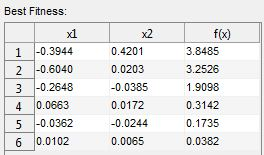
\includegraphics[scale=0.55]{ES_ackley_table.jpg}
\caption{Tabela com os melhores indivíduos de cada geração e o valor da função objetivo avaliada}
\label{fig:table}
\end{figure}


\begin{figure}[!htcb]
\centering
\includegraphics[scale=0.55]{ES_ackley_3D.eps}
\caption{Função Ackley minimizada com Estratégias Evolutivas - Melhor Indivíduo de cada geração}
\label{fig:ES_ackley_3D}
\end{figure}

\begin{figure}[!htcb]
\centering
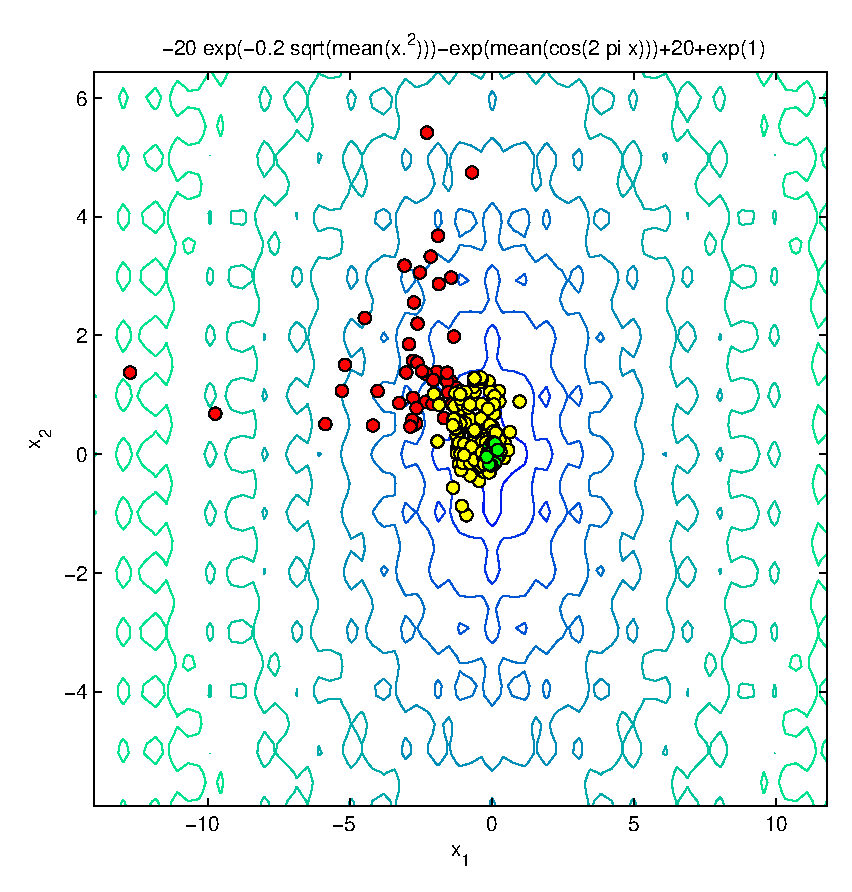
\includegraphics[scale=0.55]{ES_ackley_curvNivel.eps}
\caption{Função Ackley minimizada com Estratégias Evolutivas - Curva de Nível e indivíduos das populações}
\label{fig:ES_ackley_curvNivel}
\end{figure}

\begin{figure}
\centering
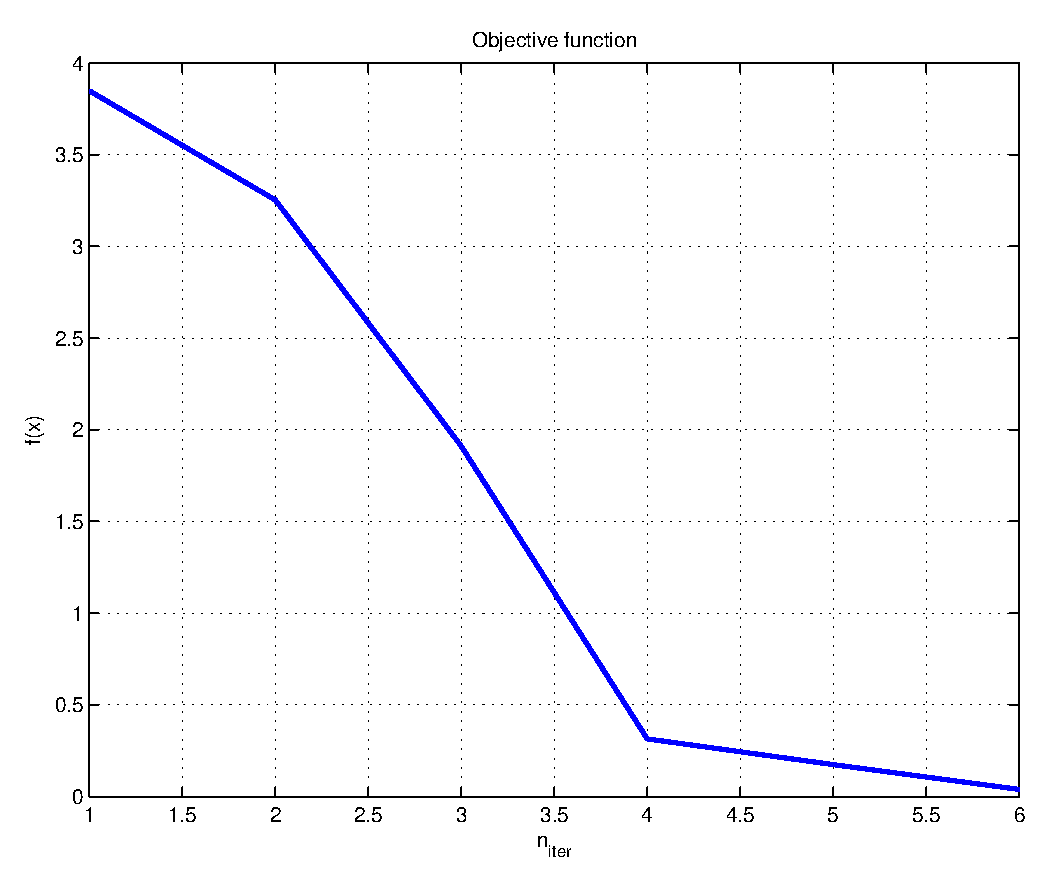
\includegraphics[scale=0.45]{ES_ackley_f.eps}
\caption{Evolução da Função Ackley avaliada para o melhor indivíduo da população em cada geração}
\label{fig:ES_ackley_f}
\end{figure}

\subsection{Simulated Annealing}


\begin{thebibliography}{1}

\bibitem{IEEEhowto:kopka}
H.~Kopka and P.~W. Daly, \emph{A Guide to \LaTeX}, 3rd~ed.\hskip 1em plus
  0.5em minus 0.4em\relax Harlow, England: Addison-Wesley, 1999.

\end{thebibliography}





\end{document}

